\documentclass[openany]{book}
\usepackage[a4paper,tmargin=25.4mm,bmargin=25.4mm,lmargin=25mm,rmargin=30mm]{geometry}
% \usepackage[margin=1cm]{geometry}
\usepackage[utf8]{inputenc}
\usepackage{listings}
\usepackage{float}
\usepackage{graphicx}
\usepackage{amsmath}
\usepackage{amsfonts}
\usepackage{array}
\usepackage[table]{xcolor}
\usepackage{multirow}
\usepackage{txfonts}
\usepackage{hyperref} 
\usepackage{subcaption} 
\usepackage[RPvoltages]{circuitikz}
\usepackage{enumitem}
\usepackage{fancyhdr}

\newcommand{\eq}{=}

\pagestyle{fancy}
\fancyhf{}
\fancyfoot[C]{\hyperlink{contents}{Ir al Contenido}}
\renewcommand{\headrulewidth}{0pt} % Si no quieres una línea en el encabezado
\renewcommand{\footrulewidth}{0pt} % Si no quieres una línea en el pie de página

\definecolor{micolor1}{HTML}{C9D7F8}
\definecolor{micolor2}{HTML}{F2F5FF}

\setcounter{secnumdepth}{3}

\title{Programming stuff}
\author{Sebastian Cortes}
\date{June 2021}

\begin{document}

\tableofcontents
\hypertarget{contents}{}


% 
\chapter{Latex}

\section{clases de documento \texttt{documentclass}}

\raggedright  \texttt{\textbackslash documentclass['opcion1', 'opcion2', ...]\{clase de documento\}} \\

  Definición de la clase de documento, en función del tipo de documento a escribir.

\subsection*{Tipos de documentos}

\subsubsection{\texttt{book}}

Para libros y otros documentos más largos que deben incluir capítulos, prólogo, apéndices o incluso partes.

\subparagraph{nota:}
\raggedright Para poder incluir un capítulo (\texttt{ \textbackslash chapter}) es necesario cambiar el tipo de documento, el tipo \texttt{\textbackslash documentclass \{ article \} } no soporta capítulos. En cambio usar \texttt{book}

\subsubsection{\texttt{article}}

Para artículos académicos y otros documentos cortos que no es necesario dividir en capítulos, sino que bastan las secciones y subsecciones y sus párrafos y subpárrafos.

\subsubsection{\texttt{report}}

Para informes técnicos. Es similar a la clase \texttt{book}

\paragraph{Nota:}  son muy similares, y ambas sirven para documentos grandes, como lo son, naturalmente, los libros y los reportes, entre otros trabajos. Sin embargo, existen ligeras diferencias. Por ejemplo, la clase \texttt{book} hace que los capítulos empiecen siempre en una página impar, de modo que si un capítulo anterior termina en una página impar, la página (par) siguiente quedará en blanco y el capítulo nuevo comenzará después de ella. Esto, en cambio, no sucede con la clase report, así es que un capítulo simplemente empieza en una página nueva, sea par o impar.

\subsubsection{\texttt{memoir}}

\subsubsection{\texttt{beamer}}

\subsection*{Opciones}

\subsubsection{tamaño de papel}

\begin{itemize}
    \item \texttt{a5paper} 210mm x 148mm
    \item \texttt{a4paper} 
    \item \texttt{b5paper} 250mm x 148mm
    \item \texttt{legalpaper} (14in x 8.5in)
    \item \texttt{executivepaper} (10.5in x 7.25in)
\end{itemize}
\paragraph{nota:} El valor por defecto es letterpaper, de Estados Unidos y México. En los documentos de otros países puede ser necesaria la opción a4paper.

\subsubsection{\texttt{landscape}} Pone la página de forma horizontal.
\subsubsection{\texttt{10pt, 11pt, 12pt}} Definen el tamaño de la fuente principal.
\subsubsection{\texttt{oneside, twoside}} Indican si el documento debe estar adaptado a impresión por un sólo lado de la página o por ambos lados de ella.
\subsubsection{\texttt{oneside, twoside}} Indican si el documento debe estar adaptado a impresión por un sólo lado de la página o por ambos lados de ella.
\subsubsection{\texttt{titlepage, notitlepage}} Determinan si el documento debe o no incluir una página de título, i.e. si va a incluir o no una portada.
\subsubsection{\texttt{openright, openany}} openright obliga a los capítulos a iniciar siempre sólo en páginas impares, mientras que con la opción openany permitimos que los capítulos se inicien en cualquier página.
\subsubsection{\texttt{onecolumn, twocolumn}} Definen si el documento se va a escribir en una sola columna o a doble columna.

\subsubsection{\texttt{fleqn}} Esta opción hace que las ecuaciones queden alineadas por la izquierda en lugar de que sean centradas (como sucede por defecto).
\subsubsection{\texttt{leqno}} Con esta opción hacemos que el número de las ecuaciones quede alineado por la izquierda en lugar de por la derecha (como sucede por defecto).
\subsubsection{\texttt{draft, final}} La opción draft se usa si queremos que la compilación del documento se haga a modo de "borrador". Con draft haremos que las líneas que sean demasiado largas queden marcadas mediante cajas negras. La opción final producirá simplemente que el documento se compile de manera normal.

\section{Paquetes \texttt{usepackage}}

\subsection{geometry}
Ofrece unas herramientas para configurar el tamaño y el diseño de diferentes elementos como tamaño del papel, márgenes, notas de pie de página, cabecera. \\\

\texttt{ \textbackslash usepackage[legalpaper, landscape, margin=2in]\{geometry\} } \\\

Es equivalente a\\\ 

\texttt{\textbackslash usepackage\{geometry\}}
\texttt{geometry\{legalpaper, landscape, margin=2in\}}\\\

Lo más importante de este paquete es cambiar el tamaño de las márgenes. Ejemplo:

\raggedright \texttt{\textbackslash usepackage[tmargin=25.4mm,bmargin=25.4mm,lmargin=30mm,rmargin=30mm]\{geometry\}}

\section{Algunos comandos}

\subsection{General}

\subsubsection{\texttt{\textbackslash makebox[ancho][pos]\{material\}}}

Es una caja de texto sin marco, los argumentos optativos Ancho y Posición denotan, respectivamente, el ancho de la caja y la posición de Material dentro de ella; éste último puede tomar los valores l, r, c, s, correspondiendo a left, right, center, y stretched (estirado). Con la opción s, los elementos de Material se separan lo más posible, hasta agotar el ancho de la caja.

Ejemplo de \makebox[5cm][r]{caja 5cm derecha} espacio.\\
Ejemplo de \makebox[5cm][l]{caja 5cm izquierda} espacio\\
Ejemplo de \makebox[5cm][c]{caja 5cm centrada} espacio\\
Ejemplo de \makebox[5cm][s]{caja 5 cm estirada} espacio\\



\subsubsection{\texttt{\textbackslash framebox[Ancho][Posición]{Material}}}

Es una caja enmarcada igual a la anterior.\\


Ejemplo de \framebox[5cm][r]{caja 5cm derecha} espacio.\\
Ejemplo de \framebox[5cm][l]{caja 5cm izquierda} espacio\\
Ejemplo de \framebox[5cm][c]{caja 5cm centrada} espacio\\
Ejemplo de \framebox[5cm][s]{caja 5 cm estirada} espacio\\

\subsubsection{\texttt{\textbackslash frame\{Material\}}}

Es un cuadro más ajustado

Ejemplo de \frame{caja sin espacio} espacio.\\


\subsubsection{\texttt{\textbackslash parbox[Posición][Alto][PosRel]\{Ancho\}\{Material\}}}

Un ejemplo de este estilo para un \fbox{
\parbox[c][2cm][c]{2cm}{Cuadro de dos cm cuadrado}}


Otro ejemplo de este estilo para un \fbox{
\parbox[b][2cm][t]{2cm}{Cuadro de dos cm cuadrado}}


Otro ejemplo de este estilo para un \fbox{
\parbox[t][2cm][b]{2cm}{Cuadro de dos cm cuadrado}}

\fbox{\parbox[c][4cm][c]{0.6\linewidth}{Condent}}
\fbox{\parbox[c][4cm][c]{0.2\linewidth}{C}}


\subsection{Ecuaciones}

\subsubsection{\texttt{\textbackslash  begin\{gathered\}}}

Sirve para centrar las ecuaciones.



\section{Advertencias}

\subsection{\texttt{Overfull \textbackslash hbox}}

Sale porque hay secuencias de caracteres o palabras muy largas según las directivas del documento. se arregla (por ahora) anteponiendo \texttt{\textbackslash raggedright}

\section{Errores}


\section{Guía para llenar bibliografia}


\subsection{Páginas de internet}
\begin{verbatim}

@misc{zzprb,
    title       = {título},
    url         = {https://www.ncbi.nlm.nih.gov/books/NBK525974/},
    journal     = {StatPearls [Internet].},
    publisher   = {quien lo publica}
}
\end{verbatim}
% \chapter*{C}

\section*{Fundamentales}

En C y en C++, una macro es una porción de código que se traduce en tiempo de preproceso.

Cuando se realiza un programa en C o C++, existen varias etapas (varios pasos), entre escribir el código fuente y tener un programa ejecutable, y finalmente ejecutamos el programa. En conjunto las llamamos compilación, pero realmente consta de cuatro etapas, más la ejecución:

\begin{enumerate}
    \item preproceso
    \item compilación
    \item ensamble
    \item enlace
    \item ejecución
\end{enumerate}

\subsection*{Macros} Se ejecutan en el preproceso y sirven para varias cosas.

\subsection*{Directivas}

\subsubsection{\texttt{\#define NAME VALUE}} 
Es un macro de sustitución simple, indica en el preprocesador que cualquier \texttt{NAME} dentro del código será sustituido por \texttt{VALUE}. 

\subsubsection{\texttt{\#undef NAME}} 
A partir del punto en que se llama esta directiva, el preprocesador deja de entender \texttt{NAME} como macro de sstitución. \\\

Otro tipo de directivas más complejas pueden parecer funciones. Como ejemplo \\\

\texttt{\#define LOOP(var,max) for(var=0;var<max;var++) } \\\

Indica un macro de sustitución de un bucle for que puede ser utilizado muchas veces. Así en código puede haber\\\

\texttt{LOOP(i,10) \{ \\\
        printf("\% d \ n", i);  \
    \} }

\subsubsection{\texttt{\#ifndef NAME}}

Si \texttt{NAME} \textbf{no} está definida, entonces ejecute las directivas (o definiciones de constantes) que estén antes de \texttt{\#endif}

\subsubsection{\texttt{\#ifdef NAME}}

Exactamente lo mismo que lo anterior.

\subsubsection{\texttt{\#if conditional\_expression}}

Indica al preprocesador que compile o no según la condición.

\subsubsection{\texttt{\#elif conditional\_expression}}

Funciona como el \texttt{else if} de toda la vida, pero para condcionales de compilación.

\subsubsection{\texttt{\#else conditional\_expression}}

Directiva que funciona como el \texttt{else} normal aplicado a condicional de compilación.

\subsubsection{\texttt{\#warning message}}

Envía un mensaje en el proceso de preprocesamiento para idicar lo que se necesite, el preprocesamiento continúa.

\subsubsection{\texttt{\#error message}}

Envía un mensaje de error y detiene el preprocesamiento.

\subsection*{Tipos y estructuras}

\subsubsection{\texttt{struct}}

Arreglos que permiten definir tipos de variables que pueden contener varios datos del mismo tipo. Su declaración es como sigue: \\\

\texttt{struct [structure tag] \{ } \\\
\texttt{member definition;}\\\
\texttt{member definition;}\\\
\texttt{member definition;}\\\
\textbf{...}\\\
\texttt{\} [one or more structure variable]; }\\\

\texttt{[structure tag]} es el nombre o etiqueta de la estructura, \texttt{member definition;} son declaraciones de variables de diferentes tipos, pertenecen a la estructura. 

Ejemplo de estructura libro: como sigue se declara para un libro1\\\

\texttt{struct Books Book1;}\\\


\texttt{Book1.pages = 564;}\\\

donde \texttt{pages} se declaro dentro de la definición de la estructura como \texttt{int}.

Se le pueden asignar valores a una estructura a partir de una lista:

\texttt{struct list lista[] = \{ }\\\
\texttt{\{ 0value1, Avalue2, ... , AvalueN \},} \\\
\texttt{\{ 1value1, Bvalue2, ... , BvalueN \},} \\\
\texttt{\{ Mvalue1, Mvalue2, ... , MvalueN \},} \\\

Donde M es el tamaño del arreglo y N es el número de diferentes componentes de la estructura, y el retorno del valor JvalueI sería \texttt{lista[J].nameI}

\subsubsection{\texttt{static}}

Dentro de una función un estático se declara y se modifica el valor de esta variable estática. Si por ejemplo en una función, se declara un estático y en esta función se le aumenta el valor. Al llamar 5 veces la función, la variable estática terminará aumentada en 5 veces; es decir, que el valor de esta variable \textbf{permanece.}

Por otro lado las funciones estáticas solamente pueden ser accesadas dentro de su propio 'scope', por lo que si una función se declara como estática, en un archivo \texttt{file1.c}, dentro del \texttt{main.c} no se podrá acceder a esta función.

\subsubsection{\texttt{typedef}}

Es una nueva definición, dependiendo de lo que le siga, \texttt{typedef} se usa para darle un nombre a ese "nuevo tipo" de variable. Ejemplo:

\texttt{typedef struct Books \{} \\
\texttt{    char title[50];} \\
\texttt{   char author[50];} \\
\texttt{   char subject[100];} \\
\texttt{   int book\_id;} \\
\texttt{\} Book;} \\

Entonces aquí \texttt{Book} puede usarse para referirse a \texttt{struct Books} y todos los componentes que se requieran.

\texttt{Book Libro1;} \\ 
Y así susecivamente.

\subsubsection{\texttt{enum}}

Es un tipo de estructura que sirve para dar significado y nombres a números que pueden pertenecer a una categoría específica. Un ejemplo es como se muestra a continuación

\begin{verbatim}
enum State {Working = 1, Failed = 0}; 
\end{verbatim}


\begin{verbatim}
enum week{Mon, Tue, Wed, Thur, Fri, Sat, Sun};
  
int main()
{
    enum week day;
    day = Wed;
    printf("%d",day);
    return 0;
} 
\end{verbatim}

Su salida será \texttt{2}


\subsubsection{Punteros o apuntadores}

Al declarar una variable, siempre esa variable se almacena dentro de la memoria. La \textbf{LA POSICIÓN DE LA MEMORIA} es importante dentro del concepto de los punteros. Los punteros guardan direcciones de memoria. 

\texttt{int a = 10;} Guarda la variable a (que tiene un valor de 10) en la memoria, para acceder a esa posición de memoria se usa \texttt{\& a}.

\texttt{int dir\_a = \& a;} guarda en la variable \texttt{dir\_a} el número que corresponde a la dirección en la memoria donde está guardada la variable a.

Para los arreglos, el nombre de la variable es un puntero hacia el valor de la primera componente:

\texttt{p = \&p[0]} \\\
De manera equivalente \\
\texttt{*p = p[0]} \\
\texttt{(*p)+1 = p[1]} \\
y así sucesivamente.


\subsubsection{Creación de variables}

Al crear una variable dentro de una función, esta variable solo existe \textbf{en el ámbito de esa función}. 

Al declarar un puntero, el valor de esa variable puntero, es la dirección donde está guardada la variable a donde apunta.


\section*{Librerías}
\subsection*{Esp32 de espidf}

\subsubsection{driver/gpio.h}

\paragraph{\texttt{gpio\_pad\_select\_gpio(number)}}
Selecciona el pin \texttt{number} para ser cofigurado como \texttt{gpio}.

\paragraph{\texttt{gpio\_set\_direction(number,mode)}}
Selecciona el pin \texttt{gpio number} y lo establece con la configuración \texttt{mode} que puede ser las siguientes: \\

\begin{itemize}
    \item \texttt{GPIO\_MODE\_DISABLE}
    \item \texttt{GPIO\_MODE\_INPUT}
    \item \texttt{GPIO\_MODE\_OUTPUT}
    \item \texttt{GPIO\_MODE\_OUTPUT\_OD}
    \item \texttt{GPIO\_MODE\_INPUT\_OUTPUT\_OD}
    \item \texttt{GPIO\_MODE\_INPUT\_OUTPUT}
\end{itemize}

\paragraph{\texttt{gpio\_get\_level(number)}}
Retorna el valor leído del pin \texttt{number} que es una entrada.

\paragraph{\texttt{gpio\_set\_level(number,value)}}
Confogura la salida del pin \texttt{number} al valor \texttt{value}.

\subsubsection{esp\_system.h}

\paragraph{\texttt{esp\_chip\_info\_t}}
Estructura que tiene información del chip: \texttt{model, features, cores, revision}.

\paragraph{\texttt{esp\_chip\_info(esp\_chip\_info\_t out)}}
Realiza el scan del chip y escribe en la estructura \texttt{out} la información pertinente.

\subsubsection{Esp32cam: OV7670}

\paragraph{\textbf{Subrutina}: \texttt{static int ov7670\_write\_array(sensor\_t, regval\_list)}}

Tiene como entrada una estructura u objeto del tipo \texttt{*sensor} (puntero) y una estructura del tipo
\texttt{regval\_list} también un apuntador.\\
Recorre todos los registros almacenados en \texttt{regval\_list} hasta el final (\texttt{vals->reg\_num != 0xff}) o hasta que una variable llamada \texttt{ret} sea diferente de cero.

Realiza escrituras a los registros que estén en \texttt{regval\_list} mediante la subrutina \texttt{SCCB\_Write}.\\\

En el archivo se inicializan una serie de estructuras del tipo \texttt{regval\_list} que selecciona distintas configuraciones, y una serie de funciones cuyos argumentos son mayoritariamente del tipo \texttt{camera} y \texttt{feature} donde feature son objetos de configuración específicas. La mayoría de estas funciones realizan escrituras y lecturas a los registros de la cámara (\texttt{ov7670\_write\_array}) para configurarla como sea requerido.\\\

Lista de funciones:

\begin{itemize}
    \item \texttt{ov7670\_frame\_control}
    \item \texttt{reset}
    \item \texttt{set\_pixformat}
    \item \texttt{set\_framesize}
    \item \texttt{set\_colorbar}
    \item \texttt{set\_whitebal}
    \item \texttt{set\_gain\_ctrl}
    \item \texttt{set\_exposure\_ctrl}
    \item \texttt{set\_hmirror}
    \item \texttt{set\_vflip}
    \item \texttt{init\_status}
\end{itemize}

\paragraph{\texttt{int ov7670\_init(sensor\_t *sensor)}}

Asigna a cada elemento del objeto (estructura) \texttt{sensor} su correspondiente configuración estructurada arriba.

\subsubsection{Esp32cam: sccb}

Define varias constantes de configuración para implementar el protocolo $I^2S$ tal como el protocolo \texttt{SCCB} exige dentro de sus lineamientos.

\paragraph{\texttt{SCCB\_Init(pin\_sda,pin\_scl)}}

\paragraph{\texttt{SCCB\_Deinit(void)}}

\paragraph{\texttt{SCCB\_Probe(void)}}

\paragraph{\texttt{SCCB\_Read(slv\_addr,reg)}}

\paragraph{\texttt{SCCB\_Write(slv\_addr,reg,data)}}

\paragraph{\texttt{SCCB\_Read16(slv\_addr,reg)}}

\paragraph{\texttt{SCCB\_Write16(slv\_addr,reg,dat)}}

\subsubsection{FreeRTOS.h}

\paragraph{\texttt{portSWITCH\_TO\_USER\_MODE()}}

\begin{verbatim}
#include “FreeRTOS.h”
#include “task.h”
void portSWITCH_TO_USER_MODE( void );
\end{verbatim}

Esta función está destinada a usuarios avanzados y es relevante en puertos con protección de memoria. Los parámetros que se pasan a \texttt{xTaskCreateRestricted()} especifican para la tarea a ser creada cuándo debe ser una tarea de modo usuario (no privilegiada) o una tarea de modo supervisor (privilegiada). Una tarea de modo supervisor puede llamar esta directiva de macro \texttt{portSWITCH\_TO\_USER\_MODE()} para convertirse a sí mismo a una tarea de modo usuario. No admite ningún parámetro y tampoco tiene parámetro de retorno. No existe una función inversa que pueda convertir una tarea de modo usuario a modo supervisor.

\paragraph{\texttt{vTaskAllocateMPURegions()}}

\begin{verbatim}
#include “FreeRTOS.h”
#include “task.h”
void vTaskAllocateMPURegions(   TaskHandle_t xTaskToModify,
                                const MemoryRegion_t * const xRegions );
\end{verbatim}

Esta función define un conjunto de regiones de Unidad de Memoria Protegida MPU para el uso de una tarea restringida MPU. Las regiones de memoria controlada pueden ser asignadas a una tarea restringida creada por \texttt{xTaskCreateRestricted()}.

Los parámetros son

\begin{itemize}
    \item \texttt{xTaskToModify} Es el manejador de la tarea a la cual se le asigna región de memoria. El manejador se obtiene mediante el parámetro \texttt{pxCreatedTask} del constructor de tarea restringida. También la tarea puede modificarse su propio acceso a región de memoria pasando un \texttt{NULL} a este parámetro.
    \item \texttt{xRegions} Es un arreglo de estructuras \texttt{MemoryRegion\_t}, el número de regiones está dado por \texttt{portNUM\_CONFIGURABLE\_REGIONS}.
\end{itemize}

La estructura de región de memoria es la siguiente

\begin{verbatim}
typedef struct xMEMORY_REGION
{   
    void *pvBaseAddress;
    unsigned long ulLengthInBytes;
    unsigned long ulParameters;
} MemoryRegion_t;
\end{verbatim}


\paragraph{\texttt{xTaskAbortDelay()}}

\begin{verbatim}
#include “FreeRTOS.h”
#include “task.h”
BaseType_t xTaskAbortDelay( TaskHandle_t xTask );
\end{verbatim}

Al llamar una función API que contenga un parámetro de tiempo timeout puede resultar que la tarea que llame esta función se boquee. Si una tarea está en estado bloqueado significa que está esperando que transcurra un periodo de tiempo timeout, o esperando con el tiempo a que ocurra un evento, para que vuelva al estado de listo. Hay dos ejemplos:

\begin{itemize}
    \item Si una tarea llama a \texttt{vTaskDelay()}, esta entrará en el estado de bloqueado hasta que el tiempo especificado termine. Una vez esto pasa, la tarea pasa al estado de preparada. 
    \item Si una tarea llama a \texttt{ulTaskNotifyTake()} cuando su valor de notificación es cero, esta se bloqueará hasta que reciba una notificación o hasta que el tiempo especificado en su parámetro correspondiente se acabe, y entonces entrará la tarea al estado de preparada.
\end{itemize}

La función \texttt{xTaskAbortDelay()} moverá la tarea del estado bloqueada al estado preparada incluso si el evento que está esperando no ha ocurrido o el tiempo especificado no ha terminado.

Mientras que una tarea esté bloqueada, no estará disponible para el planificado y por lo tanto no consumirá recursos de procesamiento.

Parámetros

\begin{itemize}
    \item \texttt{xTask} Es el manejador de la tarea. Esta se obtiene al crear la tarea especificando el manejador en su parámetro \texttt{pxCreatedTask} correspondiente, también se obtiene al crear la tarea con \texttt{xTaskCreateStatic()} y guardando el valor de retorno, o también llamando la función \texttt{xTaskGetHandle()} cuyo parámetro es el nombre de la tarea. 
\end{itemize}

El valor de retorno será un \texttt{pdPASS} si la tarea en cuestión fue removida del estado bloqueado, si no, el valor retornado será un \texttt{pdFAIL}. El valor de \texttt{INCLUDE\_xTaskAbortDelay} deberá ser de 1 en la cabecera de configuración para que la función esté disponible.

\paragraph{\texttt{xTaskCallApplicationTaskHook()}}

\begin{verbatim}
#include “FreeRTOS.h”
#include “task.h”
BaseType_t xTaskCallApplicationTaskHook( TaskHandle_t xTask, void *pvParameters );
\end{verbatim}

Es una función es destinada para usuarios avanzados. Esta función puede ser usada para asignarle un valor de 'etiqueta' a la tarea. El significado y uso de la etiqueta estarán determinados por el programador.


\paragraph{\texttt{xTaskCheckForTimeOut()}}

\begin{verbatim}
#include “FreeRTOS.h”
#include “task.h”
BaseType_t xTaskCheckForTimeOut(TimeOut_t * const pxTimeOut,
                                TickType_t * const pxTicksToWait );
\end{verbatim}

Esta función está destinada para usuarios avanzados. Una tarea puede entrar al estado bloqueado para esperar por un evento. Típicamente la tarea no va a esperar en el estado bloqueada indefinidamente, sino que a cambio será especificado un periodo de tiempo timeout. La tarea se removerá del estado bloqueado si el periodo de tiempo se termina antes de que el evento que la tarea está esperando ocurra.\\

Si una tarea entra y sale del estado bloqueado más de una vez mientras está esperando a que el evento ocurra entonces el plazo de tiempo usado cada vez que la tarea se bloquea debe ser ajustado para asegurar que el tiempo total empleado en el estado bloqueado no exceda el tiempo originalmente especificado. \texttt{xTaskCheckForTimeOut()} realiza el ajuste teniendo en cuenta las ocurrencias ocasionales, como los desbordamientos del conteo de ticks, que de otro modo harían que un ajuste manual fuera propenso a errores.\\

\texttt{xTaskCheckForTimeOut()} se usa en conjunto con \texttt{vTaskSetTimeOutState()}. Esta últimia se llama para establecer la condición inicial, luego la primera función puede ser llamada para verificar una condición de tiempo timeout, y ajustar el bloque de tiempo restante si el plazo de tiempo no ha ocurrido.

Parámetros 

\begin{itemize}
    \item \texttt{pxTimeOut} Es un puntero hacia la estructura que contiene la información necesaria para determinar si se va terminado un tiempo timeout. se inicializa mediante \texttt{vTaskSetTimeOutState()}.
    \item \texttt{pxTicksToWait} Se usa para pasar un bloque de tiempo ajustado, el cual es el bloque de tiempo que resta después de tomar en cuenta el tiempo que ya ha sido gastado en el estado bloqueado.
\end{itemize}

La función retorna un \texttt{pdTRUE} significa que no hay un bloque de tiempo restante, y el periodo de tiempo timeout se gastó todo. Si la función retorna un \texttt{pdFALSE} entonces algún bloque de tiempo queda restante por lo que no se ha acabado el plazo de tiempo.

ver \texttt{ex\_vTaskSetTimeOutState.c}

\paragraph{\texttt{xTaskCreate()}}

\begin{verbatim}
#include “FreeRTOS.h”
#include “task.h”
BaseType_t xTaskCreate( TaskFunction_t pvTaskCode,
                        const char * const pcName,  
                        unsigned short usStackDepth,
                        void *pvParameters,
                        UBaseType_t uxPriority,
                        TaskHandle_t *pxCreatedTask );
\end{verbatim}

Crea una nueva instancia de una tarea. Cada tarea utiliza memoria RAM para mantener el estado de la tarea, y es usada como la pila de la tarea. Todas las tareas que se crean están inicialmente en el estado 'preparadas' pero inmediatamente pasan al estado 'ejecutando' si no hay tareas con mayor prioridad preparadas para ejecutarse. Las tareas pueden ser creadas antes o después que el planificador inicializa.\\

\begin{itemize}
    \item \texttt{pvTaskCode} Puntero hacia la función que determina la tarea.
    \item \texttt{pcName} Nombre de la tarea 
    \item \texttt{usStackDepth} Número de palabras que la pila de la tarea podrá albergar. El tamaño será el ancho de stack de la aquitectura multiplicado por este número en bytes.
    \item \texttt{pvParameters} Los parámetros o variables de entrada de la función de la tarea. 
    \item \texttt{uxPriority} Prioridad de la tarea. Desde cero hasta \texttt{configMAX\_PRIORITIES – 1}. Se recomienda usar un número pequeño de prioridades para no malgastar RAM.
    \item \texttt{pxCreatedTask} Puede ser usada para pasar a un manejador de la tarea creada. Este manejador puede ser utilizado para hacer referencias a la tarea en llamados API para, por ejemplo, cambiar la prioridad de la tarea o borrar la tarea.
\end{itemize}


Retornos:

\begin{itemize}
    \item \texttt{pdPASS} Valor booleano que indica que la tarea fue exitosamente creada.
    \item \texttt{errCOULD\_NOT\_ALLOCATE\_REQUIRED\_MEMORY} Indica que la tarea no pudo ser creada por insuficiencia de memoria disponible.
\end{itemize}

\paragraph{\texttt{xTaskCreateRestricted()}}
\begin{verbatim}
#include “FreeRTOS.h”
#include “task.h”
BaseType_t xTaskCreateRestricted(   TaskParameters_t *pxTaskDefinition,
                                    TaskHandle_t *pxCreatedTask );
\end{verbatim}          

Esta función está enfocada para usuarios avanzados y solamente es relevante cuando se implementa un puerto FreeRTOS MPU (con unidad de protección de memoria).\\

Crea una nueva instancia de una tarea restringida con protección de memoria.

Los parámetros son
\begin{itemize}
    \item \texttt{TaskParameters\_t} Es un puntero hacia la estructura que define la tarea
\end{itemize}


\paragraph{\texttt{vTaskDelay()}}

\begin{verbatim}
#include “FreeRTOS.h”
#include “task.h”
void vTaskDelay( TickType_t xTicksToDelay );
\end{verbatim}


Bloquea la tarea que llama la función durante la cantidad de interrupciones de ticks especificada en su argumento. Si se especifican cero ticks la tarea no se bloqueará sino que dará como resultado que la tarea llamante ceda el paso a cualquier tarea de igual prioridad a que esté en el estado preparada.\\

Hacer \texttt{vTaskDelay(0)} es equivalente a \texttt{taskYIELD()}.


\paragraph{\texttt{vTaskDelayUntil()}}

\begin{verbatim}
#include “FreeRTOS.h”
#include “task.h”
void vTaskDelayUntil( TickType_t *pxPreviousWakeTime, TickType_t xTimeIncrement );
\end{verbatim}

Esta funcióon bloquea la tarea hasta que se alcance un tiempo absoluto. as tareas periódicas pueden usar esta función para conseguir una frecuencia de ejecución constante.

Las diferencias entre esta función y \texttt{vTaskDelay()} son las siguientes:

\texttt{vTaskDelay()} tiene como resultado que la tera entre en estado de bloqueo y se mantenga así en este estado, la cantidad de ticks especificado en su argumento, desde que se llama la función. Esto quiere decir que el tiempo en el que la tarea sale del estado bloqueado es \textbf{relativo} al momento en que se llama la función.

\texttt{vTaskDelayUntil()} bloquea la tarea y la mantiene bloqueada, hasta que una cantidad \textbf{absoluta de tiempo} se alcanza. Y no es relativo al momento de llamada.

Argumentos

\begin{itemize}
    \item \texttt{pxPreviousWakeTime} Este parámetro se nombra bajo el supuesto de que \texttt{vTaskDelayUntil()} está siendo utilizada para implementar una tarea que se ejecuta periódicamente y con una frecuencia fija. En este caso \texttt{pxPreviousWakeTime} contiene el tiempo en el que la tarea dejó por última vez el estado bloqueado (o en el que se 'despertó'). Este dato se usa como punto de referencia para establecer el tiempo en el que la tarea se va a volver a bloquear en el periodo siguiente.
    La variable a la que apunta \texttt{pxPreviousWakeTime} se actualiza automáticamente dentro de la función \texttt{vTaskDelayUntil()}. <No debería ser modificada dentro del código de aplicación, excepto cuando se inicializa por primera vez la variable.
    \item \texttt{xTimeIncrement} Este parámetro también esta dispuesto para el caso de una tarea periódica. La frecuencia fijada está configurada por el valor \texttt{xTimeIncrement}. Este valor está especificado en ticks. Se recomienda el uso de la macro \texttt{pdMS\_TO\_TICKS()}
\end{itemize}



\paragraph{\texttt{vTaskDelete()}}

\begin{verbatim}
#include “FreeRTOS.h”
#include “task.h”
void vTaskDelete( TaskHandle_t pxTask );
\end{verbatim}

Esta función elimina la instancia de una tarea previamente creada mediante \texttt{xTaskCreateStatic()} o \texttt{xTaskCreate()}. Se recomienda no tratar de usar el manejador de una tarea para referenciar una tarea que has sido eliminada.\\

Cuando una tarea de elimina es responsabilidad de la tarea inactiva (idle) liberar la memoria que ha sido utilizada por la tarea borrada. Por lo tanto, si una aplicación hace uso de la función \texttt{vTaskDelete()}, es muy importante que la aplicación también se asegure de que la tarea idle no esté privado de tiempo de procesamiento. Se le debe asignar tiempo de ejecución a la tarea idle.

Solamente la memoria asignada por el kernel es automáticamente liberada una vez se elimina la tarea. La memoria u otro recurso que la aplicación (distinta al kernel) asignada a la tarea debe ser liberada explícitamente por la app cuando la tarea se borra.

Argumentos 

\begin{itemize}
    \item \texttt{pxTask} Es el manejador de la tarea que se va a borrar. Una tarea se puede borrar a sí misma; en este caso, se pasa \texttt{NULL} en este argumento.
\end{itemize}

\paragraph{\texttt{taskDISABLE\_INTERRUPTS()}}


\begin{verbatim}
#include “FreeRTOS.h”
#include “task.h”
void taskDISABLE_INTERRUPTS( void );
\end{verbatim}


Si el puerto de FreeRTOS no hace uso de las constantes de configuración \texttt{configMAX\_SYSCALL\_INTERRUPT\_PRIORITY} o \texttt{configMAX\_API\_CALL\_INTERRUPT\_PRIORITY}, entonces al llamar a la función \texttt{taskDISABLE\_INTERRUPTS()} se dejarán las interrupciones gobalmente desactivadas. 

Si el sistema operativo sí hace uso de las constantes mencionadas arriba, entonces al usar la función, las interrupciones cuya prioridad estén por debajo de \texttt{configMAX\_SYSCALL\_INTERRUPT\_PRIORITY} quedarán desactivadas, y las que están por encima, activadas.t




\section*{Errores}
\paragraph{Segmetation fault} Este error se produce cuando se intenta acceder a una posición de memoria que está prohibido porque no está asignado para el programa.



% \chapter{Python}

\section{Fundamentos}

\subsection{Scope y variables del entorno}

El término "scope" en el contexto de la programación se puede traducir al
español como "ámbito" o "alcance". El alcance o ámbito de una variable en
Python se refiere a la región del programa donde esa variable es válida y puede
ser accedida.

En Python, existen diferentes niveles de alcance, como el alcance global y el
alcance local. El alcance global se refiere a las variables que están definidas
fuera de cualquier función o clase y son accesibles desde cualquier parte del
programa. El alcance local se refiere a las variables que están definidas
dentro de una función o clase y solo son accesibles dentro de esa función o
clase. El ejemplo más claro puede ser visto a continuación

\begin{verbatim}
enemies = 1

def increase_enemies():
    enemies = 2
    print("enemies is", enemies)

increase_enemies()
print("enemies is", enemies)
\end{verbatim}

En este caso se llama a una función que cambia la variable "enemies" de 1 a 2.
Sin embarago, la salida de este programa es

\begin{verbatim}
enemies is 2
enemies is 1
\end{verbatim}

Podemos ver que fuera de la función, que fue donde se declaró la variable
\texttt{enemies} esta no cambió de valor; solamente fue cambiada dentro de la
función. Si por ejemplo tratáramos de escribir un programa que declare una
variable solamente dentro de la función y la intentamos imprimir fuera de ella,

\begin{verbatim}
def drink():
    var = 1
    print(var)


print(var)
\end{verbatim}

Saltará un error \texttt{NameError: name 'var' is not defined}. Esto es porque
en este caso y en el anterior, las variables \texttt{enemies} y \texttt{var}
son variables locales y están dentro del ámbito o alcance de la función que las
declara o modifica.\\

Por su parte, cualquier variable declarada fuera de todas las funciones y
clases, son denominadas como variables locales y el ámbito o alcance de estas
será global. Y es accesible desde cualquier parte del programa. Este concepto
de ámbito o alcance no solamente aplica para las variables sino que también
aplica para funciones, entre otro tipo de elementos.

\subsubsection{Espacio de nombres}

El concepto de espacio de nombres hace referencia a la manera que se tiene de
organizar los diferentes nombres; sean de clases, funciones, variables, etc.
Cada espacio de nombre puede ser visto como un contenedor con todos los nombres
definidos. Existen diferentes tipos de namespaces:

\begin{enumerate}
    \item Namespace Global: Es el namespace de nivel superior y contiene los
          nombres definidos en el alcance global, es decir, fuera de cualquier función o
          clase. Los nombres definidos en el namespace global son accesibles desde
          cualquier parte del programa.
    \item Namespace Local: Es el namespace creado cuando se define una función
          o clase. Contiene los nombres definidos dentro de esa función o clase y solo
          son accesibles desde su interior.
    \item Namespace de Módulo: Cada archivo de Python se considera un módulo y
          tiene su propio namespace. Los nombres definidos en un módulo son accesibles
          desde otros módulos si se realiza una importación.
    \item Namespace Incorporado (Built-in): Contiene los nombres predefinidos
          que son proporcionados por Python de manera predeterminada. Estos nombres
          incluyen funciones y tipos incorporados como print(), len(), str(), etc.
\end{enumerate}

Una característica impotante de Python es que no tiene un ámbito de bloque, a
diferencia de otros lenguajes de programación. Esto quiere decir, por ejemplo,

\begin{verbatim}
if var1:
    <code>
    <code>
    <code>
    <code>
\end{verbatim}

Si el lenguaje tiene ámbito de bloque, entonces cualquier definicion dentro de
las líneas subordinadas al \texttt{if} anterior solamente existirán dentro del
\texttt{if}. En python esto no pasa, cualqueir variable que este definida aquí
estará dentro del ambito en que se encuentre el \texttt{if}.

\subsubsection{Cómo modificar una variable global}

Una cosa importante dentro del tema de los entornos de que siempre que tenemos
dos ámbitos diferentes; por ejemplo el entorno global y un entrono local, una
variable global comparada con una variable local son dos variables
completamente diferentes, aunque tengan el mismo nombre. ES muy mala idea
nombrar dos variables con el mismo nombre, aunque estén en dos ámbitos
diferentes. En el caso dado de que se requiera modificar el valor de una
variable global dentro de una variable local, es imprescindible indicar
exlícitamente que se trata de una variable global:

\begin{verbatim}
var = 2
def fun():
    global var
    var = 1
    print(var)
fun()
print(var)
\end{verbatim}

En este caso, no se crea una nueva variable en el entorno local de la función,
sino que se modifica la variable global declarada al principio.

En general no es muy recuente el uso de este método de cambio de variables
globales, porque se presta para confusiones y facilita de ciera manera los
erroes. Sin embargo, el uso de las variables globales es importante por ejemplo
cuando se necesita declarar una variable constante dentro del programa. Siempre
se usa como convención usar letras mayúsculas y barras bajas para declarar
constantes dentro del programa (ejemplo \texttt{MY\_EMAIL = "sebas@unal.edu"}).

\section{Tipos de datos, estructuras, objetos incorporados, funciones}

\subsection{variables y su almacenamiento}

al entrar en una funcion, normalmente el entorno se reinicia, con lo cual la
mayoría de las variables que se declaren o se modifiquen solamente lo hará en
ese entorno. Sin embargo, algunas funciones de algunos tipos de datos
(mayoritariamente modificar) como \texttt{list.append()}

\subsection{Funciones}

Una manera de especificar mejor los argumentos de las funciones, es mediante la
siguiente fórma:

\texttt{my\_fun(a=1, b=2, c=3)}

\subsection{Tupla}

De manera similar que una secuencia de caracteres, una tupla es una secuencia
de datos de distintos tipos. Colección de distintos datos. Este no se puede
modificar una vez se declara. Esto es, no son mutables y por tanto se almacenan
en un solo bloque de memoria.\\\

\texttt{tupla = (2,"hola",False)} \\\

Si se suman las tuplas \texttt{a} y \texttt{b}, el resultado es una
concatenación \\\

\texttt{tupla = (1,2,3)} \\
\texttt{tupla2 = (4,5,True)} \\
\texttt{tupla3 = tupla + tupla2} \\
\texttt{print(tupla3)} \\
La salida es\\
\texttt{(1,2,3,4,5,True)}\\\

Multiplicar una tupla:

\begin{verbatim}
a = (1,2)
print(a*5)
\end{verbatim}
\begin{lstlisting}
output: (1, 2, 1, 2, 1, 2, 1, 2, 1, 2)
\end{lstlisting}

Recorrer una tupla:
\begin{verbatim}
for i in tuple:
    print(i)
\end{verbatim}

Verificar si es miembro

\begin{verbatim}
    3 in (1,2,3)
\end{verbatim}

La tuplas son útiles para hacer cambios de variables en una linea misma: \\\

\texttt{x = 2}\\
\texttt{y = 5}\\
\texttt{(x,y) = (y,x)}\\
\texttt{print(x)}\\
\texttt{output: 5}\\\

También para definir una función en la que retornan varios valores

\begin{verbatim}
def funcion(x,y):
    q = x // y
    r = x % y
    return (q,r)
    
(cociente,residuo) = funcion(47,11)
print(residuo)
\end{verbatim}
\begin{lstlisting}
output: 3
\end{lstlisting}

Para retornar el enésimo elemento de una tupla se pone \texttt{tuple[i]}.
Recordar que los índices van dede cero hasta \texttt{length(tuple)-1}.

\textbf{Nota:} \texttt{tuple[1:5]} retornará los valores de la tupla desde el
índice \textbf{2} hasta el \textbf{4}.

\begin{itemize}
    \item \texttt{len(tuple)}: Retorna el tamaño de la tupla
    \item \texttt{max(tuple)}: Retorna el valor máximo de la tupla. Si en la
          tupla hay cadenas de caracteres, tuplas o listas, retorna un error.
    \item \texttt{tuple(List)}: Retorna una tupla conformada con los elementos
          de la lista List.
\end{itemize}

\subsection{Lista}

Otro tipo de arreglo de datos es la lista. La principal diferencia entre tupla
y lista es que la lista sí es mutable y también ocupa dos bloques de memoria;
esto hace que trabajar con tuplas sea más rápido pero la ventaja de la lista es
que es modificable.

\begin{verbatim}
    list1 = ['physics', 'chemistry', 1997, 2000]
\end{verbatim}

El tipo de acceso de los elementos de una lista es el mismo que para las
tuplas. De la misma forma las operaciones; ver la sección anterior en las
operaciones de listas. \\\

\subsubsection{Lista de funciones}

\paragraph{\texttt{len(list)}} Retorna el tamaño de la lista.
\paragraph{\texttt{max(list)}} Retorna el valor del máximo, si la lista
contiene combinaciones de numeros y caracteres o listas o tuplas, genera error.
\paragraph{\texttt{min(list)}} Retorna el valor mínimo dentro de la lista.
\paragraph{\texttt{list(seq)}} Retorna una lista compuesta por los elementos de
\texttt{seq}.
\paragraph{\texttt{sorted(list)}} Retorna una lista con los elementos de
\texttt{list} ordenados de menor a mayor.

\subsubsection{Lista de métodos}

\paragraph{\texttt{list.append(obj)}} Añade el objeto \texttt{obj} al final de
la lista

\paragraph{\texttt{list.count(obj)}} Retorna el número de veces que el objeto
\texttt{obj} ocurre en la lista.

\paragraph{\texttt{list.extend(seq)}} Añade el contenido de \texttt{seq} a la
lista. Lo añade al final de la lista.

\paragraph{\texttt{list.index(obj)}} Retorna el índice más pequeño en la lista
en que el objeto \texttt{obj} aparece.

\paragraph{\texttt{list.insert(index, obj)}} Inserta el objeto \texttt{obj} en
la casilla \texttt{index} de la lista, moviendo el resto una posición.

\paragraph{\texttt{list.pop(obj = list[-1])}} Remueve y retorna el objeto que
se encuentre en la posición \texttt{obj}. Por defecto si no se ingresa
argumento, remueve el último objeto de la lista.

\paragraph{\texttt{list.remove(obj)}} Remueve el primer objeto \texttt{obj} que
encuentre en la lista.

\paragraph{\texttt{list.reverse()}} Invierte el orden de los componentes de la
lista.

\paragraph{\texttt{list.sort(key=None)}} Organiza los elementos de la lista, si
hay una directiva de oredenamiento, se puede ingresar como el argumento
\texttt{key}, por defecto, organiza de menor a mayor.

\paragraph{\texttt{list.clear(}} Elimina todos los componentes dentro de la
lista dejándola como una lista vacía.

\paragraph{\texttt{list.copy()}} Retorna una copia de la lista.

\subparagraph{Nota} Si se declara una lista como sigue
\begin{verbatim}
    A = [1,2,3]
    B = A
\end{verbatim}
Tanto \texttt{A} como \texttt{B} están apuntando al mismo objeto, o dirección
de memoria. Para realizar una copia de \texttt{A} en otro espacio de memoria se
utiliza

\begin{verbatim}
    B = A[:]
\end{verbatim}

\subsection{Diccionario}

Es una lista especial en la que se puede dar un identificador especial al
índice de la misma

\begin{verbatim}
    dict = {'Name': 'Zara', 'Age': 7, 'Class': 'First'}
    print(dict["Name"])
\end{verbatim}

El primer objeto del diccionario tiene un identificador llamado "Name" y un
valor asociado a él que en este caso es "Zara". La salida del código anterior
será

\begin{verbatim}
    Zara
\end{verbatim}

Se puede modificar el valor de una entrada en el diccionario y se puede también
añadir una nueva entrada

\begin{verbatim}
    dict = {'Name': 'Zara', 'Age': 7, 'Class': 'First'}
    dict['Age'] = 8; # update existing entry
    dict['School'] = "DPS School" # Add new entry
\end{verbatim}

Para borrar elementos de un diccionario

\begin{verbatim}
    del(dict["Name"])
\end{verbatim}

Una propiedad importante de los diccionarios es que los elementos pueden ser
cualquier objeto de python. Las 'llaves' o identificadores deben ser objetos
inmutables como cadenas de caracteres o tuplas.

\subsubsection{Funciones}

\paragraph{\texttt{len(dic)}}

\paragraph{\texttt{srt(dic)}} Retorna una cadena de caracteres imprimible de
los elementos que contiene el diccionario \texttt{dic}

\subsubsection{Métodos}

\paragraph{\texttt{dic.clear()}}

\paragraph{\texttt{dic.copy()}}

\paragraph{\texttt{dic.fromkeys(iterable,value)}} Retorna un nuevo diccionario
cuyas 'llaves' estarán determinadas por los elementos de \texttt{iterable} y
con un valor asociado (único) de \texttt{value}

\paragraph{\texttt{dic.get(key, default=None)}} Retorna el valor
correspondiente a la llave \texttt{key}. El segundo argumento es el retorno
cuando no hay una llave que corresponda.

\paragraph{\texttt{dic.items()}} Este método retorna una lista de tuplas, cada
tupla corresponde a la llave y al valor correspondiente.

\paragraph{\texttt{dic.keys()}} Retorna una vista de todas las llaves del
diccionario. Se puede conseguir la lista nativa a través de \texttt{list()}.

\paragraph{\texttt{dic.setdefault(key, default = None)}} Es similar a
\texttt{get()} con la diferencia de que si la llave \texttt{key} no está en el
diccionario, entonces la añade y su valor correspondiente será \texttt{default}

\paragraph{\texttt{dic.update(dict2)}} Actualiza el diccionario añadiendo todos
los pares (llave-valor) de \texttt{dict2}.

\paragraph{\texttt{dic.values()}} Retorna una vista de los valores del
diccionario. Se puede conseguir la lista nativa a través de \texttt{list()}.

\subsection{\texttt{open()}}

El retorno de esta función es un objeto \texttt{file}.

\begin{verbatim}
open (file, mode='r', buffering=- 1, encoding=None, errors=None, newline=None, closefd=True, opener=None)
\end{verbatim}

\begin{itemize}
    \item \texttt{file} es un objeto \texttt{path-like}, es el nombre del
          archivo a abrir (incluyendo la ruta si es necesario) o crear.
    \item \texttt{mode} es un string opcional que especifica el modo en el que
          el archivo se abre, por defecto \texttt{'r'} para leer \texttt{'w'} para
          escribir, truncando el archivo primero \texttt{'x'} para creación de archivo
          nuevo, falla si ya hay un archivo con ese nombre, \texttt{'a'} para escribir en
          el archivo, anexando al final del archivo si este existe, \texttt{'b'} modo
          binario, \texttt{'t'} es modo de texto que está por defecto, \texttt{'+'} para
          abrir y actualizar (leer y escribir)
\end{itemize}

Los archivos abiertos en el modo binario retornan el contenido como objetos
byte sin ninguna decodificación; en el modo texto, el contenido se lee como
string.

\subsubsection{Concatenación especial de cadenas de caracteres.}

una forma interesante de hacer concatenación de caracteres es mediante la
siguiente forma. Sea \texttt{score=0} una variable del tipo \texttt{int}. Si
hacemos \texttt{print(f"your score is {score}")} se hará la conversión de
entero a caracter automáticamente sin la necesidad de hacer \texttt{print("your
    score is" + str(score)")}

\section{Errores y debuggeo de los mismos}

\subsection{Tipos de testeo}

\subsubsection{Test unitario}

Si el programa es modular, es posible hacer tests que aseguren que cada función
hace lo que se supone que debe hacer según las especificaciones.

\subsubsection*{Test de regresión}

Cada vez que se soluciona un error, se realiza testeo nuevamente del código,
con el objetivo de asegurarse que al realizar la corrección no se agregaron
nuevos errores.

\subsubsection*{Test de integración}

Realizar testeo del programa como un todo. Se ponen juntas cada una de las
partes individuales

\subsubsection{back box testing}

Se tiene el código y se realizan las pruebas con diferentes casos con el fin de
encontrar todas las rutas posibles que hay en el código.

Se determina el docstring de una función, ejemplo: \\

\begin{verbatim}
    def sqrt(x,eps)
        """Asume x y eps como flotantes, mayores que cero o igual para x, y retorna un res tal que x-eps <= res <= x+eps
\end{verbatim}

La idea es entonces realizar testeos de diferentes casos dadas las
especificaciones del docstring.

En el caso del ejemplo anterior, se puede hacer un conjunto de pruebas con
valores como raíces cuadradas perfectas, números irracionales, menores que 1, o
por ejemplo con valores extremos como muy pequeño y muy grandes de ambos
\texttt{x} y \texttt{eps}.

\subsubsection{glass box testing}

En este caso lo que se hace es utilizar directamente el código para guiar los
casos de prueba. En este caso se pueden llegar a presentar muchas posibilidades
de caminos disponibles, teniendo en cuenta la posible presencia de bucles y
repeticiones en el código.
Pr ejemplo, para ramas en los que hay diferentes casos, es importante lograr
hacer la prueba para todos y cada uno de los posibles caminos o casos. Para
bucles \texttt{for}, se deben preparar pruebas en las que no se entra a dicho
bucle, también pruebas en las que se entra una vez, dos veces, tres y así
sucesivamente. Para bucles \texttt{while} es de manera similar, pero
asegurándose de tener casos de prueba que puedan cubrir todas la formas
posibles de romper el bucle.

Hacer el debugging tiene una variedad grande de posibilidades. Utilizar
\texttt{print}, por ejemplo, dentro de funciones o bucles.

\subsection{Errores}

\subsubsection{\texttt{IndexError}}

\begin{verbatim}
    test[1,2,3]
    test[4]
\end{verbatim}

\subsubsection{\texttt{TypeError}}

\texttt{int(test)}

\subsubsection{\texttt{NameError}} cuando no se encuentra un nombre ya sea
local o global.

\texttt{a}
una variable inexistente.

\subsubsection{\texttt{SyntaxError}}

Errores de sintaxis. Cuando python no puede interpretar o analizar
gramaticalmente el código.

\subsubsection{\texttt{AttributeError}} las referencias a atributos falla.

\subsubsection{\texttt{ValueError}} el tipo de operador está correcto, pero el
valor del mismo es imposible.

\subsubsection{\texttt{IOError}} El sistema IO reporta una malfunción (por
ejemplo un archivo no encontrado). Los errores son llamados excepciones.

ahora por alguna razón esto no deja seguir y continuar

\subsection{Handlers}

Los llamados manejadores, son lo que se encargan de llevar a cabo la rutina o
ejecución necesaria cuando determinada cosa ocurre, sean interrupciones o
excepciones.

\begin{verbatim}
    try:
        xxxxxxx
        xxxxxx
    except (exception_type1):
        xxxxxx
        xxxxx
    except (exception_type2):
        xxxxxx
        xxxxx
        .
        .
        .
\end{verbatim}

\begin{verbatim}
    else:
\end{verbatim}

lo anterior se ejecuta cuando el cuerpo del \texttt{try} asociado se ejecuta
sin ninguna excepción.

\begin{verbatim}
    finally:
\end{verbatim}

Siempre se ejecuta después del \texttt{try}, \texttt{else}, y \texttt{except},
incluso cuando existen \texttt{break}, \texttt{continue} o \texttt{return}.

\begin{verbatim}
    raise <ExceptionName> (<Arguments>)
    raise <ValueError> ("Uis, algo esta mal")
\end{verbatim}

\subsection{assertions}

programación "defensiva".

\begin{verbatim}
    assert <lo_que_se_espera>, <mensaje>
\end{verbatim}

Da un error de ejecución del tipo \texttt{AssertError}. dando la explicación
pertinente.

Ahora hay errores lógicos que son más complicados de tratar.

Cosas que no se deben hacer:

\begin{enumerate}
    \item Escribir el código entero para hacer pruebas sobre él
    \item Hacer debug en el programa entero
    \item Olvidar en qué lugar estaba el bug
    \item Olvidar cuáles fueron los cambios que se hicieron
\end{enumerate}

Por el contrario es más recomendable escribir una función, probarla, hacer
depuración, y así con cada función nueva que se escriba. Hacer Testeo de
integración.
También hacer copias de seguridad del código, cambiarlo, advertir mediante
comentarios los cambios, y al realizar pruebas, hacer comparaciones.

\section{POO}

\texttt{object} es el tipo más básico en python.

\begin{verbatim}
    class <name>(<parent_class>):
\end{verbatim}

\begin{verbatim}
    class coordinate(object):
        def __init__(self, x, y):
            self.x = x
            self.y = y
\end{verbatim}

El \texttt{self} es un parámetro para referirse a la instancia de la clase, la
que esté ejecutándose. El constructor siempre será \texttt{def
    \_\_init\_\_():}\\

\subsection{Métodos importantes}

Estos métodos sustituyen operadores o funciones importantes.

\begin{itemize}
    \item \texttt{\_\_str\_\_():} Su retorno es lo que se muestra cuando se
          ejecuta la función \texttt{print()}
    \item \texttt{\_\_add\_\_():} Su retorno es el valor de 'a+b'.
    \item \texttt{\_\_sub\_\_():} Su retorno es el valor de 'a-b'.
    \item \texttt{\_\_mul\_\_():} Su retorno es el valor de 'a*b'.
    \item \texttt{\_\_eq\_\_():} Su retorno es el valor de 'a==b'.
    \item \texttt{\_\_lt\_\_():} Su retorno es el valor de 'a<b'.
    \item \texttt{\_\_len\_\_():} Su retorno es el valor de 'len(a)'.
\end{itemize}

\textbf{nota} las \textbf{variables de clase} son variables cuyo valor se
comparte entre todas las instancias de la clase

\section{Sobre algoritmos}

¿Cómo se puede establecer o sabe qué tan eficiente es mi algoritmo?

Los razonamientos que surgen a partir de este punto dan como resultado un
análisis interesante sobre las siguientes cuestiones:

\begin{itemize}
    \item Cómo podemos razonar sobre un algoritmo con el objetivo de predecir
          la cantidad de tiempo que este necesitará para resolver un problema de un
          tamaño en particular.
    \item Cómo podemos relacionar las opciones en el diseño de algoritmos con
          la eficiencia en tiempo del resultado.
\end{itemize}

\section{Pandas}

En el contexto de la biblioteca `pandas` en Python, un **dataframe** es una
estructura de datos bidimensional, similar a una tabla en una base de datos,
una hoja de cálculo o una tabla en lenguajes estadísticos como R. Es
esencialmente una colección ordenada de columnas, donde cada columna puede
tener un tipo de dato diferente (número, cadena, booleano, etc.).

El término "data tabular" se refiere precisamente a este tipo de datos en forma
de tabla, donde:

\begin{itemize}
    \item Las \textit{filas} representan observaciones o entradas individuales.
    \item Las \textit{columnas} representan características o variables de esas
          observaciones.
\end{itemize}

Matemáticamente, podríamos considerar un dataframe como una matriz \( M \) de
dimensiones \( m \times n \), donde \( m \) es el número de filas y \( n \) es
el número de columnas. Cada elemento \( M_{ij} \) representa el valor en la
i-ésima fila y j-ésima columna.

Un dataframe en `pandas` proporciona una serie de funcionalidades útiles para
manipular y analizar datos tabulares, tales como:

\begin{enumerate}
    \item Operaciones de filtrado y selección basadas en condiciones.
    \item Agrupaciones y operaciones de agregación.
    \item Fusiones y uniones con otros dataframes.
    \item Operaciones de pivote y reestructuración.
    \item Funcionalidades para manejo de datos faltantes.
    \item  Integración con otras bibliotecas de Python como `numpy`, `scipy` y
          `matplotlib`.
\end{enumerate}1.

Para ilustrar esto con un pequeño ejemplo, considera el siguiente dataframe:

\[
    \begin{array}{|c|c|c|}
        \hline
        \textbf{Nombre} & \textbf{Edad} & \textbf{Profesión} \\
        \hline
        Juan            & 30            & Ingeniero          \\
        \hline
        Ana             & 25            & Doctora            \\
        \hline
        Carlos          & 28            & Arquitecto         \\
        \hline
    \end{array}
\]

En este dataframe:
Las filas representan a diferentes individuos.
Las columnas representan características de estos individuos: su nombre, edad y
profesión.

La facilidad con la que `pandas` permite manipular, filtrar y analizar este
tipo de datos ha hecho que sea una herramienta esencial para cualquier persona
que trabaje con análisis de datos en Python.

\subsection{\texttt{Funciones de entradas y salidas}}

Estas son las funciones mediante las cuales se pueden obtener diferentes
objetos de pandas o guardar como salidas.

\subsubsection{\texttt{pandas.read\_csv()}}

Esta función es una de las más utilizadas porque importa directamente un
archivo \texttt{csv} y lo convierte en un \texttt{DataFrame} (en la siguiente
sección se hablará de este objeto)

\paragraph{Parámetros}

\subparagraph{\texttt{filepath\_or\_buffer}}

\begin{itemize}
    \item \textbf{Descripción:} Es la ruta del archivo \textit{csv} a importar.
          Se puede usar una URL
    \item \textbf{Tipo:} \texttt{str}. También acepta objetos tipo
          \texttt{PathLike} u objetos \texttt{path}.
\end{itemize}

\subparagraph{\texttt{sep}}

\begin{itemize}
    \item \textbf{Descripción:} El tipo de separador de los datos, normalmente
          son comas \texttt{','} , pero puede ser configurado según el archivo que se va
          a importar.
    \item \textbf{Tipo:} \texttt{str}.
    \item \textbf{Por defecto:} \textit{','}
\end{itemize}

\subparagraph{\texttt{header}}

\begin{itemize}
    \item \textbf{Descripción:} Es la especificación de la fila que contiene
          las etiquetas de las columnas. Por defecto siempre será la primera.
    \item \textbf{Tipo:} \texttt{int} , \texttt{infer} o \texttt{None}. Si se
          especifica \texttt{None}, las etiquetas de las columnas serán índices desde 0
          hasta n. Si se especifica \texttt{infer}, se asume que	\texttt{header = 0}
    \item \textbf{Por defecto:} \textit{infer} .
\end{itemize}

\subparagraph{\texttt{index\_col}}

\begin{itemize}
    \item \textbf{Descripción:} Especifica la columna que se usará como
          etiquetas de las filas.
    \item \textbf{Tipo:} \texttt{hashable}. Comúnmente suelen ser del tipo
          numérico (\texttt{int} o \texttt{float}) o cadenas de caracteres \texttt{str}.
          Básicamente es la etiqueta de la columna que se usará como etiqueta
    \item \textbf{Por defecto:}  Es opcional.
\end{itemize}

\subparagraph{\texttt{usecols}}

\begin{itemize}
    \item \textbf{Descripción:} Se puede seleccionar un conjunto de columnas
          para importar y descartar las demás. Este parámetro especifica este conjunto
    \item \textbf{Tipo:} Lista de \texttt{hashables}.
    \item \textbf{Por defecto:} Es opcional.
\end{itemize}

% \subparagraph{\texttt{}}
% \begin{itemize}
%     \item \textbf{Descripción:}
%     \item \textbf{Tipo:}
%     \item \textbf{Por defecto:}
% \end{itemize}

% \subparagraph{\texttt{}}
% \subparagraph{\texttt{}}

\subsection{Funciones generales}

\subsubsection{Filtrado de información}

Existen varios métodos para filtrar los datos de un \texttt{dataframe}. Los más
básicos son los que solamente tienen una condición. También están las múltiples
condiciones.

\paragraph{Una sola condición:} Si un dataframe con nombre \texttt{df} tiene
una columna cuya etiqueta o nombre es \texttt{sex}; una forma de filtrar sería
la siguiente:

\begin{verbatim}
                    df[df.sex == "male"]
                    \end{verbatim}

De esta manera se obtiene o se retorna un dataframe con la información
filtrada.

Por su parte, se puede utilizar el método \texttt{loc} para realizar el
filtrado:

\begin{verbatim}
                    df.loc[df.sex == "male"]    
                    \end{verbatim}

Y si por ejemplo, se quiere solamente se requiere sacar una columna, se usa
\begin{verbatim}
                    df.loc[df.sex == "male", "fare"]    
                    \end{verbatim}

\paragraph{Varias condiciones:}

Una forma de filtrar por el tipo de variable en el dataframe, en este caso se
seleccionan una o más columnas

\begin{verbatim}
                    mask = df.dtypes == "int64"
                    df.loc[mask]    
                    \end{verbatim}

Se pueden definir diferentes máscaras, tanto para las filas como para las
columnas.

\begin{verbatim}
                    mask1 = df["age"] >= 55
                    mask2 = df.dtypes == "int64"
                    df.loc[mask]    
                    \end{verbatim}

Adicionalmente se pueden usar funciones lógicas para mejorar la precisión del
filtro:
\begin{verbatim}
                    df.loc[(df.sex == "male") & (df.age > 25)]    
                    \end{verbatim}

Existen algunas reglas adicionales para máscaras para filtrar de forma más
práctica:

\begin{verbatim}
                    mask = summer["Year"].between(1960, 1984, inclusive = True)
                    mask2 = summer["Year"].isin([1972,1996])
                    \end{verbatim}

Este último es útil para seleccionar explícitamente un conjunto de elementos a
filtrar, seleccionándolas o extrayéndolas mediante la negación. El argumento
siempre es una lista con los objetos que quiero filtrar.

\subsubsection{ELiminación de filas y columnas}

Existen varias formas de eliminar filas y columnas de los dataframes. La forma
más básica es mediante el método \texttt{drop}. Este método tiene el parámetro
\texttt{inplace}

\begin{verbatim}
            df.drop(columns = "col")    
            \end{verbatim}

Para eliminar más de una columna, se pasa una lista con las etiquetas
correspondientes como argumento.

\begin{verbatim}
            df.drop(columns = ["col1", "col2"])    
            \end{verbatim}

Dos alternativas para eliminar una columna son las siguientes.

\begin{verbatim}
            df.drop(labels = "col_name", axis = "columns")
            del df["col"]
            \end{verbatim}

Para eliminar las filas se utiliza la misma forma, reemplazando
\texttt{columns} por \texttt{index}. Con esta forma se eliminan todas las
instancias con el índice seleccionado, en caso que haya más de una fila con el
mismo índice.

\begin{verbatim}
            df.drop(index = index_name)
            \end{verbatim}

Otra forma es renombrando el dataframe con una versión filtrada de la misma

\begin{verbatim}
            df = df.loc[df.col == value]
            \end{verbatim}

Aquí se seleccionan solamente las filas cuyo valor para la columna \texttt{col}
es \texttt{value}, descartando todas las otras.

Si creamos diferentes máscaras, y luego filtramos la negación lógica de dichas
máscaras, entonces estaremos eliminando las filas que cumplan con la máscara o
máscaras.

\begin{verbatim}
            mask1 = summer["Year"] == 2012
            mask2 = summer["Country"] == "RUS"
            summerf = summer.loc[~(mask1 & mask2)]
            \end{verbatim}

\subsubsection{Añadidura de columnas}

La forma más básica de añadir una nueva columna es asignando un valor constante
a dicha columna

\begin{verbatim}
            df["col_nueva"] = 0
            \end{verbatim}

Si \texttt{col\_nueva} no existe, entonces se creará y se llenará con el valor
0 para todos los índices. Si la columna ya existe, entonces se reemplazarán
todos los valores con la nueva asgnación. Por su parte, si se crea una columna
de la siguiente forma

\begin{verbatim}
            df.new_col = 0
            \end{verbatim}

En realidad se creará un nuevo atributo para el dataframe, con valor 1, pero no
se creará una columna.\\

Si se utiliza una operación tradicional con una columna del dataframe, se
creará una columna nueva, y esto se puede utilizar para añadir columnas nuevas
con base en datos de otras columnas:

\begin{verbatim}
            titanic["yob"] = 1912 - titanic["age"]
            \end{verbatim}

Para añadir una nueva columna en una posición específica, se utiliza el método
\texttt{insert}:

\begin{verbatim}
            col_new = df[col] + 3
            df.insert(loc = 6, column = "new_col_name", value = col_new)
            \end{verbatim}

De esta forma se asegura que la columna nueva sea localizada en la sexta
posición. Las columnas que estén a la derecha serán desplazadas una posición.

Por otro lado, también se pueden añadir entradas nuevas o filas nuevas.
Asignando una lista o iterable concordante con el data frame, a un nuevo
índice.

\subsubsection{Manupulación de valores}

Se puede cambiar un solo valor mediante el atributo \texttt{loc} y también
\texttt{iloc}

\begin{verbatim}
            titanic.loc["index","col"] = 40
            titanic.iloc[1,1] = 40
            \end{verbatim}

\noindent Para cambiar varios valores puede hacerse de la siguiente forma

\begin{verbatim}
            titanic.loc[1:3, "age"] = 42
            \end{verbatim}

\noindent Se puede cambiar un rango específico de valores con una lista de
valores compatible:

\begin{verbatim}
            titanic.iloc[1:4, 3] = [43,44,45]
            \end{verbatim}
\noindent Recordar que con el comando \texttt{loc} si el índice es numérico, se
selecciona incluyendo desde el primer número hata el último, mientras que con
\texttt{iloc} se seleccionar el índice de forma tradicional como si se tratara
de una lista.

\noindent Para reemplazar o cambiar valores basado en condiciones, se usa la
siguiente forma
\begin{verbatim}
            titanic.loc[titanic.age < 1, "age"]
            \end{verbatim}
\noindent Por su parte, si se requiere cambiar más de una columna para una
entrada (fila) en particular se puede usar el siguiente código
\begin{verbatim}
            titanic.loc[0,"survived":"age"] = [1, 2, "female", 24.0]
            \end{verbatim}

\noindent El método \texttt{replace} es útil cuando queremos reemplazar todas
las entradas que cumplan una condición
\begin{verbatim}
            titanic.replace(0, "zero")
            \end{verbatim}

\noindent Esto reemplaza todos los ceros que haya en la tabla por el texto
"zero". \\\

\noindent Es crucial entender que al declarar una variable como referencia a
una columna de una tabla, en realidad estamos creando un apuntador a dicha
columna. Esto significa que cualquier cambio o reemplazo de valores en esta
variable implicará una modificación directa en la columna correspondiente de la
tabla:
\begin{verbatim}
            edad = titanic.age
            edad.loc[1] = 40 # aquí
            \end{verbatim}
\noindent En el reemplazo de variables dentro de una tala la manera correcta de
realizarlo es como se mencionó en la sección anterior, realizarlo de otra forma
se considera una mala práctica:
\begin{verbatim}
            titanic.loc[1,"age"] = 40 # esta es forma correcta
            titanic.age[1] = 40 # esta no se debe relizar
            \end{verbatim}
\noindent Por otro lado, si se asigna a una variable una o más columnas
poniendo una lista como argumento, dicha variable si se modifica, no modificará
la tabla original.
\begin{verbatim}
            sexo = titanic[["sex"]]
            sexo.loc[0] = "ajefemalee"
            sexo.iloc[0] = "ajefemalee" # también aplica para iloc
            titanic # no tendrá el valor modificado
            \end{verbatim}
\noindent Si se utiliza el campo para el índice \texttt{[:]} obtendremos el
mismo resultado; sin embargo, al modificar una variable declarada de esta
forma, Pandas no generará ninguna advertencia.
\begin{verbatim}
            sexo = titanic.loc[:,["sex"]]}            
            \end{verbatim}
Ahora, si se intenta reemplazar valores mediante la notación de doble
paréntesis, como se muestra a continuación
\begin{verbatim}
            titanic[titanic["age"] < 1]["age"] = 1
            \end{verbatim}
\noindent La tabla no será cambiada, y se mostrará una advertencia. Cuando se
ejecuta \texttt{titanic[titanic["age"] < 1]["age"]}, se está realizando dos
operaciones de indexación consecutivas. Primero, \texttt{titanic[titanic["age"]
            < 1]} crea una vista o una copia temporal filtrada del \texttt{DataFrame
    titanic}, seleccionando solo las filas donde \texttt{age} es menor que 1.
Luego, \texttt{["age"]} selecciona la columna \texttt{age} de esta vista o
copia temporal. Al intentar asignar un nuevo valor a esta selección, se está
modificando la copia temporal y no la tabla original.
\noindent Pero, si se realiza una selección de la columna primero, y luego se
realiza el filtro,
\begin{verbatim}
            titanic["age"][titanic["age"] < 1] = 1
            \end{verbatim}
La tabla sí será modificada. Esto es debido a la forma en que se realiza la
indexación y asignación en este caso específico. En Pandas, cuando se hace una
indexación directa sobre una columna del \texttt{DataFrame}, como en
\texttt{titanic["age"]}, se obtiene una vista directa de esa columna en el
\texttt{DataFrame} original, no una copia. Esta vista es una referencia a los
datos en la columna \texttt{age} dentro del \texttt{DataFrame titanic}. Luego,
cuando se aplica un filtro adicional con \texttt{[titanic["age"] < 1]}, se está
seleccionando ciertas posiciones de esa vista, y cualquier cambio que hagas
aquí se reflejará en el \texttt{DataFrame} original. Al asignar \texttt{= 1} a
esta selección, se está modificando directamente los datos en la columna
\texttt{age} del \texttt{DataFrame titanic}. Es importante notar que, aunque
esta forma de indexación y asignación puede funcionar, no es la recomendada, ya
que puede llevar a confusión y a errores sutiles, especialmente en contextos
más complejos. \\\

\noindent En conclusión, es importante tener claridad sobre cuándo se está
realizando una vista de un conjunto de datos tomados de una tabla (apuntador a
la columna, o conjunto de datos) y cuándo se está realizando una copia (sea
temporal o no) de los datos; la copia es un objeto completamente independiente
de la tabla original. Si se selecciona una columna mediante la notación de
atributo (\texttt{titanic.age}) o mediante la notación de paréntesis cuadrados,
o cualquier otra notación, es fácil y muy útil utilizar el atributo
\texttt{\_is\_view} y el método \texttt{\_is\_copy()}.

\paragraph{Consejos de buena práctica:} En general, según el propósito que se
tenga, es conveniente y recomendado utilizar cierto tipo de métodos y atributos
a la hora de manipular datos de una tabla.
Si se requiere trabajar y manipular la tabla entera, entones el consejo es
evitar el indexado encadenado. La indexación encadenada en Pandas se refiere al
proceso de realizar varias operaciones de indexación sucesivas, una tras otra,
típicamente utilizando corchetes \texttt{[]}. Esto suele verse en la forma de
\texttt{dataframe[...][...]}, donde se realizan dos (o más) operaciones de
indexación de forma secuencial. Por su parte, si se desea trabajar con
porciones de la tabla, es recomendado realizar una copia de dicha porción
mediante el método \texttt{copy()} y trabajar sobre esta.

\subsubsection{Métodos de ordenamiento}

\noindent La manera clásica de ordenar una tabla basado en una columna es la
siguiente
\begin{verbatim}
            titanic.sort_values(by = "age")
            \end{verbatim}
Recordar que la línea anterior retorna la tabla ordenada, no modifica la
actual, para hacer esto se debe usar el parámetro \texttt{inplace}. Recordar
también el parámetro \texttt{ascending}.

\noindent Se puede hacer ordenamiento no solamente por una columna sino por
varias, pasando la lista con las etiquetas de las columnas como argumento del
parámetro \texttt{by}. La columna de la primera etiqueta de la lista que se
pasa como argumento es la que tiene la primera prioridad. También se puede
pasar una lista booleana especificando cuáles se ordenarán de forma ascendente
y cuáles descendente.
\begin{verbatim}
            titanic.sort_values(by = ["col1", "col2", "col3"], ascending = [True False False], inplace = True)
            \end{verbatim}
\noindent Siempre se puede reordenar la tabla con base en el índice de las
filas:
\begin{verbatim}
            titanic.sort_index(ascending = True, inplace = True)
            \end{verbatim}
Cuando se realiza un ordenamiento basado en una columna, los índices también se
ordenan o "desordenan". En algunas ocasionoes se requiere que el índice
prevalezca ordenado aun cuando la tabla completa cambió con el ordenamiento.
Esto se logra con dos formas distintas:
\begin{verbatim}
            titanic.sort_values(by = age).reset_index(drop = True)
            titanc.sort_values(by = "age", ignore_index = True)
            \end{verbatim}

\subsubsection{Estadísticas con agregación}

El método \texttt{agg} es utilizado para realizar operaciones de agregación
sobre una tabla, permitiendo aplicar una o más funciones sobre sus ejes. Se
puede especificar una función, nombre de función, lista de funciones o un
diccionario que mapea etiquetas de eje a funciones. Por defecto, estas
operaciones se realizan sobre las filas (`axis=0`), pero también pueden
aplicarse a las columnas (`axis=1`). El resultado de `agg` puede ser un
escalar, una Serie o un DataFrame, dependiendo de la operación. Una forma
efectiva de usarlo es seleccionar columnas de un tipo específico, como las
numéricas, y luego aplicar un diccionario para realizar distintas operaciones
en cada columna, tal como \texttt{df.select\_dtypes("number").agg({"col1":
"mean", "col2": ["min", "std"]})}. Esto permite realizar análisis detallados y
personalizados sobre los datos de manera eficiente.

\subsubsection{Uso de funciones definidas en las tablas}

\noindent Una funcionalidad interesante es la posibilidad de ejecutar funciones
sobre todos los elementos de una tabla. Si definimos una función
\begin{verbatim}
            def range(series):
                return series.max() - series.min()
            \end{verbatim}
\noindent Al implementar el método \texttt{apply} se puede ejecutar la función
para los elementos de la columna o los elementos de las filas, según se
establezca:
\begin{verbatim}
            sales.apply(range, axis = 0)
            \end{verbatim}
El valor de \texttt{axis = 0} es para las filas y \texttt{axis=1} para las
columnas. Retornará una tabla con el resultado de la función. \\
\noindent Se puede pasar la función lambda directamente en caso de requerir
poco cóidigo:
\begin{verbatim}
            sales.apply(lambda x: x.max() - x.min(), axis = 0)
            \end{verbatim}
Si se selecciona una sola columna o porción de ella, el intérprete ya sabe que
se ejecutará la función a dichos elementos:
\begin{verbatim}
            sales.loc[1:10,"col1"].apply(lambda x: x[0])
            \end{verbatim}
\noindent El método \texttt{map} es similar, con la diferencia de que solamente
aplica para series de datos, es decir una columna por ejemplo. Por último, Se
puede aplicar una función a toda la tabla (o parte de ella) mediante el
siguiente método.
\begin{verbatim}
            df.applymap(func)
            df.loc[1:99,"col"].applymap(func)
           \end{verbatim}

\subsubsection{Multiindexación}
En una tabla es posible que como índice, no solamente haya una columna, sino
más de una:
\begin{verbatim}
            df.set_index(["col1", "col2 "])
           \end{verbatim}
Podemos ordenar de forma personalizada los diferentes índices:
\begin{verbatim}
            df.sort__index(ascending = [True False])
            \end{verbatim}
Como podemos ver, hay un índices exterior y uno interior, este orden puede ser
cambiado mediante el método:
\begin{verbatim}
            df.swaplevel()
            \end{verbatim}
Se puede restablecer el índice de la siguiente forma:
\begin{verbatim}
            df.reset_index(inplace = True)
            \end{verbatim}
El indexador \texttt{loc} puede ser usado de la siguiente manera para poder
extraer o filtrar información necesaria de una tabla:
si se desea filtrar ambos índices y luego ver una columna, los índices deben
ser puestos en una tupla:
\begin{verbatim}
            df.loc[(idx1,idx2), col]
            \end{verbatim}
Se puede no colocar ninguna columna y así veremos todas las columnas.
Para seleccionar más de un valor para los índices, estos e colocan dentro de
una lista. Para extraer todas las columnas, es necesario indicar los dos
puntos:
\begin{verbatim}
            df.loc[([idx1a,idx1b],idx2), col]
            df.loc[([idx1a,idx1b],idx2),:]
            \end{verbatim}
Para seleccionar todos los valores de un índice, la notación \texttt{:}
poroduce un error, por tanto se debe usar \texttt{slice(None)}:
\begin{verbatim}
            df.loc[([idx1a,idx1b],slice(None)),:]
            \end{verbatim}
\subsubsection{Operaciones con cadenas de texto}
Para todos los datos dentro de una tabla que sean cadenas de texto, si se
requiere realizar cualquier operación, se debe implementar el método
\texttt{.str}:
\begin{verbatim}
            df.str.lower()
            \end{verbatim}
Para el método \texttt{split}, se tiene la opción de separar de manera
automática el resultado en columnas separadas:
\begin{verbatim}
            summer[col].srt.split("," n = 2, expand = True)
            \end{verbatim}
El parámeto \texttt{n} indica cuántos de los caracteres separadores se requiere
tomar, y el parámetro \texttt{expand} indica si se requiere guardar el retorno
en columnas separadas. \\
También es útil utilizar métodos de string como \texttt{contains} para realizar
filtros personalizados y especializados:
\begin{verbatim}
            summer[summer["Event"].str.contains("100M")]
            \end{verbatim}

\subsection{Objeto \texttt{DataFrame}}

Es una de las clases más importantes de Pandas; una estructura de datos tabular
de dos dimensiones. Es una representación en Pandas de una tabla de datos.

\subsubsection{Constructor} El constructor es el siguiente

\begin{verbatim}
            class pandas.DataFrame(data=None, index=None, columns=None, dtype=None, copy=None)
            \end{verbatim}
\paragraph{Parámetros}

\subparagraph{\texttt{data}}
\begin{itemize}
    \item \textbf{Descripción:} Es el conjunto de datos que conformará el
          DataFrame.
    \item \textbf{Tipo:} \texttt{numpy.ndarray}, elementos iterables,
          \texttt{dict}, o \texttt{DataFrame}
    \item \textbf{Por defecto:} \texttt{None}
\end{itemize}

\subparagraph{\texttt{index}}
\begin{itemize}
    \item \textbf{Descripción:} Es el comjunto de etiquetas de las filas de la
          estructura
    \item     \textbf{Tipo:} \texttt{Index} o arreglo de índices (una lista de
          \texttt{str}).
    \item     \textbf{Por defecto:} \texttt{None}
\end{itemize}

\subparagraph{\texttt{columns}}
\begin{itemize}
    \item \textbf{Descripción:} Es el conjunto de etiquetas de las columnas de
          la estructura
    \item \textbf{Tipo:} \texttt{Index} o arreglo de índices (lista de
          \texttt{str}).
    \item \textbf{Por defecto:} \texttt{None}.
\end{itemize}

\subsubsection{Atributos}

La siguiente es la lista de los atributos de la clase \texttt{DataFrame}

\paragraph{~\hspace{2em} \texttt{T}:} La transposición del DataFrame.

\paragraph{~\hspace{2em}\texttt{at}:} Accede a un valor único para un par
etiqueta de fila/columna.

\paragraph{~\hspace{2em}\texttt{attrs}:} Diccionario de atributos globales de
este conjunto de datos.

\paragraph{~\hspace{2em}\texttt{axes}:} Devuelve una lista que representa los
ejes del DataFrame (lista de \texttt{Index}).

\paragraph{~\hspace{2em}\texttt{columns[]}:} Las etiquetas de columna del
DataFrame. Pueden indexarse como una lista.

\paragraph{~\hspace{2em}\texttt{dtypes}:} Devuelve los tipos de datos en el
DataFrame.

\paragraph{~\hspace{2em}\texttt{empty}:} Indicador de si la Serie/DataFrame
está vacío.

\paragraph{~\hspace{2em}\texttt{flags}:} Obtiene las propiedades asociadas con
este objeto pandas.

\paragraph{~\hspace{2em}\texttt{iat}:} Accede a un valor único para un par
fila/columna por posición entera.

\paragraph{~\hspace{2em}\texttt{iloc}:} Indexación basada puramente en la
ubicación por posición entera.

\paragraph{~\hspace{2em}\texttt{index[]}:} El índice (etiquetas de fila) del
DataFrame. Puede indexarse como en una lista.

\paragraph{~\hspace{2em}\texttt{loc}:} Accede a un grupo de filas y columnas
por etiqueta(s) o un array booleano.

\paragraph{~\hspace{2em}\texttt{ndim}:} Devuelve un entero que representa el
número de ejes / dimensiones del array.

\paragraph{~\hspace{2em}\texttt{shape}:} Devuelve una tupla que representa la
dimensionalidad del DataFrame.

\paragraph{~\hspace{2em}\texttt{size}:} Devuelve un entero que representa el
número de elementos en este objeto.

\paragraph{~\hspace{2em}\texttt{style}:} Devuelve un objeto Styler.

\paragraph{~\hspace{2em}\texttt{values}:} Devuelve una representación en Numpy
del DataFrame.

\begin{enumerate}
    \item\texttt{pd.options.display.min\_rows}
    \item\texttt{pd.options.display.max\_rows}
\end{enumerate}
Estas variables se modifican a conveniencia para mostrar una cantidad mínima y
máxima requerida de los datos de la tabla.

\subsubsection{Métodos}
% \paragraph{\texttt{method1}} descripción
% \subparagraph{\textbf{parámetros}}
%     \begin{itemize}
%         \item \texttt{param1}
%             \begin{itemize}
%                 \item \textbf{Descripción:}
%                 \item \textbf{Tipo:}
%                 \item \textbf{Por defecto:}
%             \end{itemize}
%     \end{itemize}

% \subparagraph{\textbf{Tipo de retorno:}}

\paragraph{\texttt{abs()}} Devuelve una Serie/DataFrame con el valor numérico
absoluto de cada elemento.
\subparagraph{\textbf{parámetros}}
\begin{itemize}
    \item \texttt{Ninguno}
\end{itemize}
\subparagraph{\textbf{Retorno:}} \texttt{pandas.Series} o
\texttt{Pandas.DataaFrame}

\paragraph{\texttt{add(other, axis, level, fill\_value)}} Obtiene la suma de
los elementos (elemento a elemento) del dataframe con otro dataframe (u objeto
similar).
\subparagraph{\textbf{parámetros}}
\begin{itemize}
    \item \texttt{other}
          \begin{itemize}
              \item \textbf{Descripción:} Objeto con el cual se realiza la
                    suma.
              \item \textbf{Tipo:} \texttt{Serie}, \texttt{DataFrame},
                    \texttt{dict} o cualquier escalar o secuencia.
              \item \textbf{Por defecto:} Ninguno
          \end{itemize}
    \item \texttt{axis}
          \begin{itemize}
              \item \textbf{Descripción:} Selecciona si comparar por el índice
                    o por la columna.
              \item \textbf{Tipo:} \texttt{0} o \texttt{'index'}, \texttt{1} o
                    \texttt{'column'}
              \item \textbf{Por defecto:} \texttt{'columns'}
          \end{itemize}
    \item \texttt{fill\_value}
          \begin{itemize}
              \item \textbf{Descripción:} Rellenar valores que potencialmente
                    serán no determinados (\texttt{NaN}). Esto es especialmente útil cuando se usan
                    dos tablas con diferentes índices y/o columnas.
              \item \textbf{Tipo:} \texttt{float} o \texttt{None}
              \item \textbf{Por defecto:} \texttt{None}
          \end{itemize}
\end{itemize}
\subparagraph{Retorno:} \texttt{DataFrame} con los resultados de los valores

\paragraph{\texttt{add\_prefix(prefix, axis)}} Añade un prefijo a las columnas.
Si la columna es \texttt{'a'} y el prefijo dado es \texttt{'col\_'}, la columna
queda etiquetada como \texttt{col\_a}. No modifica el objeto (retorna uno
nuevo)
\subparagraph{\textbf{parámetros}}
\begin{itemize}
    \item \texttt{prefix}
          \begin{itemize}
              \item \textbf{Descripción:} La cadena de texto para prefijar.
              \item \textbf{Tipo:} \texttt{String}
              \item \textbf{Por defecto:} Ninguno
          \end{itemize}
    \item \texttt{axis}
          \begin{itemize}
              \item \textbf{Descripción:} Selecciona el eje al cual añadir el
                    prefijo.
              \item \textbf{Tipo:}  \texttt{0} o \texttt{'index'}, \texttt{1} o
                    \texttt{'column'}
              \item \textbf{Por defecto:} \texttt{None}
          \end{itemize}
\end{itemize}
\subparagraph{Retorno:} \texttt{DataFrame}

\paragraph{\texttt{add\_suffix(suffix, axis)}} Añade un sufijo a las columnas.
Análogo al método anterior.
\subparagraph{\textbf{parámetros}}
\begin{itemize}
    \item \texttt{suffix}
          \begin{itemize}
              \item \textbf{Descripción:} La cadena de texto a añadir.
              \item \textbf{Tipo:} \texttt{String}
              \item \textbf{Por defecto:} Ninguno
          \end{itemize}
    \item \texttt{axis}
          \begin{itemize}
              \item \textbf{Descripción:} Selecciona el eje al cual añadir el
                    sufijo.
              \item \textbf{Tipo:} \texttt{0} o \texttt{'index'}, \texttt{1} o
                    \texttt{'column'}
              \item \textbf{Por defecto:} \texttt{None}
          \end{itemize}
\end{itemize}
\subparagraph{Retorno:} \texttt{DataFrame}

\paragraph{\texttt{agg(func, axis)}} Agrega utilizando una o más operaciones
sobre el eje especificado.
\subparagraph{\textbf{parámetros}}
\begin{itemize}
    \item \texttt{func}
          \begin{itemize}
              \item \textbf{Descripción:} La función o funciones para aplicar.
              \item \textbf{Tipo:} Función o lista de funciones (como ejemplo
                    \texttt{'sum'})
              \item \textbf{Por defecto:} Ninguno
          \end{itemize}
    \item \texttt{axis}
          \begin{itemize}
              \item \textbf{Descripción:} Eje sobre la cual realizar la
                    función, si esta última está definida para listas.
              \item \textbf{Tipo:} \texttt{0} o \texttt{'index'}, \texttt{1} o
                    \texttt{'column'}
              \item \textbf{Por defecto:} \texttt{0}
          \end{itemize}
\end{itemize}
\subparagraph{Retorno:} \texttt{DataFrame}, \texttt{Series} o puede ser
escalar, dependiendo de la función usada.

\paragraph{\texttt{align(other, join, axis, level, copy, fill\_value)}}
Alinea dos objetos en sus ejes con el método de unión especificado. El método
de unión está especificado para cada índice de eje.

\subparagraph{\textbf{Parámetros}}
\begin{itemize}
    \item \texttt{other}
          \begin{itemize}
              \item \textbf{Descripción:} DataFrame o Series con el que se
                    quiere alinear.
              \item \textbf{Tipo:} DataFrame o Series
              \item \textbf{Por defecto:} Ninguno
          \end{itemize}
    \item \texttt{join}
          \begin{itemize}
              \item \textbf{Descripción:} Tipo de alineación a realizar
                    (\texttt{'outer'}, \texttt{'inner'}, \texttt{'left'}, \texttt{'right'}).
              \item \textbf{Tipo:} Cadena de texto
              \item \textbf{Por defecto:} \texttt{'outer'}
          \end{itemize}
    \item \texttt{axis}
          \begin{itemize}
              \item \textbf{Descripción:} Eje permitido del otro objeto.
              \item \textbf{Tipo:} \texttt{0}, \texttt{1}, o \texttt{None}
              \item \textbf{Por defecto:} \texttt{None}
          \end{itemize}
    \item \texttt{level}
          \begin{itemize}
              \item \textbf{Descripción:} Difunde a través de un nivel,
                    coincidiendo con los valores del índice en el nivel MultiIndex pasado.
              \item \textbf{Tipo:} Entero o nombre de nivel
              \item \textbf{Por defecto:} \texttt{None}
          \end{itemize}
    \item \texttt{copy}
          \begin{itemize}
              \item \textbf{Descripción:} Siempre devuelve nuevos objetos. Si
                    \texttt{copy=False} y no se requiere reindexación, se devuelven los objetos
                    originales.
              \item \textbf{Tipo:} Booleano
              \item \textbf{Por defecto:} \texttt{True}
          \end{itemize}
    \item \texttt{fill\_value}
          \begin{itemize}
              \item \textbf{Descripción:} Valor a utilizar para valores
                    faltantes. Por defecto es NaN, pero puede ser cualquier valor "compatible".
              \item \textbf{Tipo:} Escalar
              \item \textbf{Por defecto:} \texttt{np.nan}
          \end{itemize}
\end{itemize}

\subparagraph{Retorno:} Tupla de (Series/DataFrame, tipo del otro objeto)
\begin{itemize}
    \item \textbf{Descripción:} Objetos alineados.
    \item \textbf{Tipo:} Tupla
\end{itemize}

\paragraph{\texttt{all(axis, bool\_only, skipna, **kwargs)}}
Devuelve si todos los elementos son \texttt{True}, potencialmente a lo largo de
un eje. Devuelve \texttt{True} a menos que haya al menos un elemento dentro de
una serie o a lo largo de un eje de DataFrame que sea \texttt{False} o
equivalente (p. ej., cero o vacío).

\subparagraph{\textbf{Parámetros}}
\begin{itemize}
    \item \texttt{axis}
          \begin{itemize}
              \item \textbf{Descripción:} Indica qué eje o ejes deben
                    reducirse. Para Series, este parámetro no se utiliza y se establece en 0 por
                    defecto.
              \item \textbf{Tipo:} \texttt{0} o \texttt{'index'}, \texttt{1} o
                    \texttt{'columns'}, \texttt{None}
              \item \textbf{Por defecto:} \texttt{0}
          \end{itemize}
    \item \texttt{bool\_only}
          \begin{itemize}
              \item \textbf{Descripción:} Incluye solo columnas booleanas. No
                    implementado para Series.
              \item \textbf{Tipo:} Booleano
              \item \textbf{Por defecto:} \texttt{False}
          \end{itemize}
    \item \texttt{skipna}
          \begin{itemize}
              \item \textbf{Descripción:} Excluye valores NA/nulos. Si toda la
                    fila/columna es NA y \texttt{skipna} es \texttt{True}, entonces el resultado
                    será \texttt{True}, como en el caso de una fila/columna vacía. Si
                    \texttt{skipna} es \texttt{False}, entonces los NA se tratan como
                    \texttt{True}, porque no son iguales a cero.
              \item \textbf{Tipo:} Booleano
              \item \textbf{Por defecto:} \texttt{True}
          \end{itemize}
    \item \texttt{**kwargs}
          \begin{itemize}
              \item \textbf{Descripción:} Palabras clave adicionales no tienen
                    efecto pero podrían ser aceptadas para compatibilidad con NumPy.
              \item \textbf{Tipo:} Cualquiera
              \item \textbf{Por defecto:} \texttt{None}
          \end{itemize}
\end{itemize}

\subparagraph{Retorno:} Series o DataFrame
\begin{itemize}
    \item \textbf{Descripción:} Si se especifica un nivel, se devuelve un
          DataFrame; de lo contrario, se devuelve una Series.
    \item \textbf{Tipo:} Series o DataFrame
\end{itemize}

\paragraph{\texttt{DataFrame.any(*, axis=0, bool\_only=False, skipna=True,
        **kwargs)}}
Devuelve si algún elemento es \texttt{True}, potencialmente a lo largo de un
eje. Devuelve \texttt{False} a menos que haya al menos un elemento dentro de
una serie o a lo largo de un eje de DataFrame que sea \texttt{True} o
equivalente (p.ej., no cero o no vacío).

\subparagraph{\textbf{Parámetros}}
\begin{itemize}
    \item \texttt{axis}
          \begin{itemize}
              \item \textbf{Descripción:} Indica qué eje o ejes deben
                    reducirse. Para Series, este parámetro no se utiliza y se establece en 0 por
                    defecto.
              \item \textbf{Tipo:} \texttt{0} o \texttt{'index'}, \texttt{1} o
                    \texttt{'columns'}, \texttt{None}
              \item \textbf{Por defecto:} \texttt{0}
          \end{itemize}
    \item \texttt{bool\_only}
          \begin{itemize}
              \item \textbf{Descripción:} Incluye solo columnas booleanas. No
                    implementado para Series.
              \item \textbf{Tipo:} Booleano
              \item \textbf{Por defecto:} \texttt{False}
          \end{itemize}
    \item \texttt{skipna}
          \begin{itemize}
              \item \textbf{Descripción:} Excluye valores NA/nulos. Si toda la
                    fila/columna es NA y \texttt{skipna} es \texttt{True}, entonces el resultado
                    será \texttt{False}, como en el caso de una fila/columna vacía. Si
                    \texttt{skipna} es \texttt{False}, entonces los NA se tratan como
                    \texttt{True}, porque no son iguales a cero.
              \item \textbf{Tipo:} Booleano
              \item \textbf{Por defecto:} \texttt{True}
          \end{itemize}
    \item \texttt{**kwargs}
          \begin{itemize}
              \item \textbf{Descripción:} Palabras clave adicionales no tienen
                    efecto pero podrían ser aceptadas para compatibilidad con NumPy.
              \item \textbf{Tipo:} Cualquiera
              \item \textbf{Por defecto:} \texttt{None}
          \end{itemize}
\end{itemize}

\subparagraph{Retorno:} Series o DataFrame
\begin{itemize}
    \item \textbf{Descripción:} Si se especifica un nivel, se devuelve un
          DataFrame; de lo contrario, se devuelve una Series.
    \item \textbf{Tipo:} Series o DataFrame
\end{itemize}

\paragraph{\texttt{head(n)}} Esta función retorna las primeras \( n \) filas
del objeto basado en su posición. Es útil para comprobar rápidamente si el
objeto contiene el tipo correcto de datos.

Para valores negativos de \( n \), esta función devuelve todas las filas
excepto las últimas \( |n| \) filas, equivalente a \( \text{df}[:n] \).

Si \( n \) es mayor que el número de filas, esta función retorna todas las
filas.

\subparagraph{\textbf{Parámetros}}
\begin{itemize}
    \item \texttt{n}
          \begin{itemize}
              \item \textbf{Descripción:} Número de filas a seleccionar.
              \item \textbf{Tipo:} Entero
              \item \textbf{Por defecto:} 5
          \end{itemize}
\end{itemize}

\subparagraph{Retorno:} Mismo tipo que el objeto que llama
\begin{itemize}
    \item \textbf{Descripción:} Las primeras \( n \) filas del objeto que llama
          la función.
    \item \textbf{Tipo:} Mismo tipo que el objeto que llama
\end{itemize}

\subparagraph{Tipo de dato de salida} \texttt{DataFrame}

\paragraph{\texttt{tail(n=5)}} Esta función retorna las últimas \( n \) filas
del objeto basado en su posición. Es útil para verificar rápidamente los datos,
por ejemplo, después de ordenar o agregar filas.

Para valores negativos de \( n \), esta función devuelve todas las filas
excepto las primeras \( |n| \) filas, equivalente a \( \text{df}[|n|:] \).

Si \( n \) es mayor que el número de filas, esta función retorna todas las
filas.

\subparagraph{\textbf{Parámetros}}
\begin{itemize}
    \item \texttt{n}
          \begin{itemize}
              \item \textbf{Descripción:} Número de filas a seleccionar.
              \item \textbf{Tipo:} Entero
              \item \textbf{Por defecto:} 5
          \end{itemize}
\end{itemize}

\subparagraph{Retorno:} Tipo del objeto que llama la función
\begin{itemize}
    \item \textbf{Descripción:} Las últimas \( n \) filas del objeto que llama
          la función.
    \item \textbf{Tipo:} Tipo del objeto que llama la función
\end{itemize}

\paragraph{\texttt{info(verbose, buf, max\_cols, memory\_usage, show\_counts)}}
Este método imprime información sobre un DataFrame incluyendo el tipo de datos
del índice y las columnas, los valores no nulos y el uso de memoria.

\subparagraph{\textbf{Parámetros}}
\begin{itemize}
    \item \texttt{verbose}
          \begin{itemize}
              \item \textbf{Descripción:} Si se imprime el resumen completo.
                    Por defecto, se sigue la configuración en
                    \texttt{pandas.options.display.max\_info\_columns}.
              \item \textbf{Tipo:} Booleano, opcional
          \end{itemize}
    \item \texttt{buf}
          \begin{itemize}
              \item \textbf{Descripción:} Dónde enviar la salida. Por defecto,
                    la salida se imprime en \texttt{sys.stdout}. Se puede pasar un búfer escribible
                    si se necesita procesar más la salida.
              \item \textbf{Tipo:} Búfer escribible, valor por defecto
                    \texttt{sys.stdout}
          \end{itemize}
    \item \texttt{max\_cols}
          \begin{itemize}
              \item \textbf{Descripción:} Cuándo cambiar de la salida detallada
                    a la salida truncada. Si el DataFrame tiene más de \texttt{max\_cols} columnas,
                    se utiliza la salida truncada.
              \item \textbf{Tipo:} Entero, opcional
          \end{itemize}
    \item \texttt{memory\_usage}
          \begin{itemize}
              \item \textbf{Descripción:} Especifica si se debe mostrar el uso
                    total de memoria de los elementos del DataFrame (incluido el índice).
              \item \textbf{Tipo:} Booleano, cadena, opcional
          \end{itemize}
    \item \texttt{show\_counts}
          \begin{itemize}
              \item \textbf{Descripción:} Si se muestran los recuentos de no
                    nulos. Por defecto, esto se muestra solo si el DataFrame es más pequeño que las
                    opciones en \texttt{pandas.options.display.max\_info\_rows} y
                    \texttt{pandas.options.display.max\_info\_columns}.
              \item \textbf{Tipo:} Booleano, opcional
          \end{itemize}
\end{itemize}

\subparagraph{Retorno:} Ninguno
\begin{itemize}
    \item \textbf{Descripción:} Este método imprime un resumen de un DataFrame
          y no devuelve nada.
    \item \textbf{Tipo:} Ninguno
\end{itemize}

\paragraph{\texttt{describe(percentiles, include, exclude)}}Genera estadísticas
descriptivas. Las estadísticas descriptivas incluyen aquellas que resumen la
tendencia central, la dispersión y la forma de la distribución del conjunto de
datos, excluyendo los valores NaN. Analiza tanto series numéricas como de
objeto, así como conjuntos de columnas de DataFrame de tipos de datos mixtos.
La salida variará dependiendo de lo que se proporcione. Consulte las notas a
continuación para obtener más detalles.

\subparagraph{\textbf{Parámetros}}
\begin{itemize}
    \item \texttt{percentiles}
          \begin{itemize}
              \item \textbf{Descripción:} Los percentiles a incluir en la
                    salida. Todos deben estar entre 0 y 1. El valor por defecto es \([.25, .5,
                            .75]\), que devuelve los percentiles 25, 50 y 75.
              \item \textbf{Tipo:} Lista de números
              \item \textbf{Por defecto:} Ninguno (Opcional)
          \end{itemize}
    \item \texttt{include}
          \begin{itemize}
              \item \textbf{Descripción:} Lista blanca de tipos de datos para
                    incluir en el resultado. Ignorado para Series.
              \item \textbf{Tipo:} ‘all’, lista de tipos de datos o Ninguno
                    (Por defecto)
              \item \textbf{Opciones:} ‘all’, lista de dtypes, Ninguno
          \end{itemize}
    \item \texttt{exclude}
          \begin{itemize}
              \item \textbf{Descripción:} Lista negra de tipos de datos para
                    omitir del resultado. Ignorado para Series.
              \item \textbf{Tipo:} Lista de tipos de datos o Ninguno (Por
                    defecto)
              \item \textbf{Opciones:} Lista de dtypes, Ninguno
          \end{itemize}
\end{itemize}

\subparagraph{Retorno:} Series o DataFrame
\begin{itemize}
    \item \textbf{Descripción:} Estadísticas resumidas de la Series o DataFrame
          proporcionado.
    \item \textbf{Tipo:} Series o DataFrame
\end{itemize}

\paragraph{\texttt{len(df)}} Retorna el número de filas que hay en la tabla.
\subparagraph{Tipo de dato de salida} \texttt{Int}

\paragraph{\texttt{round(df,0)}} Retorna la tabla con los valores numéricos
redondeados con las cifras especificadas.
\subparagraph{Tipo de dato de salida} \texttt{Int}

\paragraph{\texttt{mean(axis, skipna, numeric\_only, **kwargs)}} Calcula la
media de los valores a lo largo del eje solicitado.

\subparagraph{\textbf{Parámetros}}
\begin{itemize}
    \item \texttt{axis}
          \begin{itemize}
              \item \textbf{Descripción:} Eje sobre el que se aplica la
                    función. Para Series, este parámetro no se utiliza y su valor predeterminado es
                    0. Para DataFrames, especificar \texttt{axis=None} aplicará la agregación en
                    ambos ejes.
              \item \textbf{Tipo:} \{0 ('index'), 1 ('columns')\}
              \item \textbf{Por defecto:} \texttt{0}
          \end{itemize}

    \item \texttt{skipna}
          \begin{itemize}
              \item \textbf{Descripción:} Excluir valores NA/nulos al calcular
                    el resultado.
              \item \textbf{Tipo:} Booleano
              \item \textbf{Por defecto:} \texttt{True}
          \end{itemize}

    \item \texttt{numeric\_only}
          \begin{itemize}
              \item \textbf{Descripción:} Incluir solo columnas de tipo float,
                    int, booleano. No implementado para Series.
              \item \textbf{Tipo:} Booleano
              \item \textbf{Por defecto:} \texttt{False}
          \end{itemize}

    \item \texttt{**kwargs}
          \begin{itemize}
              \item \textbf{Descripción:} Argumentos de palabras clave
                    adicionales para pasar a la función.
              \item \textbf{Tipo:} Cualquiera
          \end{itemize}
\end{itemize}

\subparagraph{Retorno:} Series o escalar
\begin{itemize}
    \item \textbf{Descripción:} La media de los valores a lo largo del eje
          especificado.
    \item \textbf{Tipo:} \texttt{Series} o escalar
\end{itemize}

\paragraph{\texttt{sort\_values(by, *, axis, ascending, inplace, kind,
        na\_position, ignore\_index, key)}} Ordena por los valores a lo largo de
cualquiera de los ejes.

\subparagraph{\textbf{Parámetros}}
\begin{itemize}
    \item \texttt{by}
          \begin{itemize}
              \item \textbf{Descripción:} Nombre o lista de nombres (índices)
                    por los que ordenar.
              \item \textbf{Tipo:} Cadena de caracteres o lista de cadenas de
                    caracteres, según el índice.
          \end{itemize}

    \item \texttt{axis}
          \begin{itemize}
              \item \textbf{Descripción:} Eje que será ordenado.
              \item \textbf{Tipo:} \{0 ('index'), 1 ('columns')\}
              \item \textbf{Por defecto:} 0
          \end{itemize}

    \item \texttt{ascending}
          \begin{itemize}
              \item \textbf{Descripción:} Ordenar de forma ascendente vs
                    descendente. Especifique una lista para múltiples órdenes de clasificación.
              \item \textbf{Tipo:} Booleano o lista de booleanos
              \item \textbf{Por defecto:} Verdadero
          \end{itemize}

    \item \texttt{inplace}
          \begin{itemize}
              \item \textbf{Descripción:} Si es Verdadero, aplica el
                    ordenamiento al objeto.
              \item \textbf{Tipo:} Booleano
              \item \textbf{Por defecto:} Falso
          \end{itemize}

    \item \texttt{kind}
          \begin{itemize}
              \item \textbf{Descripción:} Elección del algoritmo de ordenación.
              \item \textbf{Tipo:} \{'quicksort', 'mergesort', 'heapsort',
                    'stable'\}
              \item \textbf{Por defecto:} 'quicksort'
          \end{itemize}

    \item \texttt{na\_position}
          \begin{itemize}
              \item \textbf{Descripción:} Ubica los NaN al principio si es
                    'first'; al final si es 'last'.
              \item \textbf{Tipo:} \{'first', 'last'\}
              \item \textbf{Por defecto:} 'last'
          \end{itemize}

    \item \texttt{ignore\_index}
          \begin{itemize}
              \item \textbf{Descripción:} Si es Verdadero, el eje resultante se
                    etiquetará 0, 1, ..., n - 1.
              \item \textbf{Tipo:} Booleano
              \item \textbf{Por defecto:} Falso
          \end{itemize}

    \item \texttt{key}
          \begin{itemize}
              \item \textbf{Descripción:} Aplicar la función clave a los
                    valores antes de ordenar.
              \item \textbf{Tipo:} Función
              \item \textbf{Opcional:} Verdadero
          \end{itemize}
\end{itemize}

\subparagraph{Retorno:} DataFrame o None
\begin{itemize}
    \item \textbf{Descripción:} DataFrame con valores ordenados o None si
          \texttt{inplace=True}.
    \item \textbf{Tipo:} DataFrame o None
\end{itemize}

\paragraph{Selección de columnas}

Si se tiene un DataFrame, podemos usar el índice \texttt{[]} para seleccionar
una o más columnas diferentes.

\begin{verbatim}
                    df["col1"]
                    \end{verbatim}
Una forma alternativa es mediante la notación de punto:

\begin{verbatim}
                    df.col1
                    \end{verbatim}
Si queremos obtener más de una columna, debemos ingresar las etiquetas de
dichas columnas como una \textbf{lista}:
\begin{verbatim}
                    df[["col1","col2"]]
                    \end{verbatim}
\subparagraph{Tipo de dato de salida} Si se pone solamente la etiqueta de una
columna como argumento, el tipo de retorno será \texttt{Series}. Si se pone una
lista de una o más etiquetas, entonces la salida será otro \texttt{DataFrame}.

\paragraph{\texttt{df.iloc[n,m]}} Este método retorna la información de la fila
enésima y columna enésima. Se pueden seleccionar una o más filas/columnas, y si
se requiere un conjunto específico de filas/columnas, deben ingresarse dentro
de una lista
\begin{verbatim}
                    df.iloc[25:30]
                    df.iloc[25,2]
                    df.iloc[25:30,2:5]
                    df.iloc[[100,345,778],[0,4]]
                    \end{verbatim}
\subparagraph{Tipo de dato de salida} \texttt{Series, DataFrame} o el tipo de
objeto en la celda, cuando se especifica una sola celda.

\paragraph{\texttt{df.loc[Rlabel,Clabel]}} Este método es muy similar al
anterior, con la diferencia de que se asigna como argumento el texto de la
etiqueta de la fila que se desea retornar. Si hay más de una fila con la misma
etiqueta, entonces se retornan todas las filas.

\subparagraph{Tipo de dato de salida} \texttt{Series, DataFrame} o el tipo de
objeto en la celda, cuando se especifica una sola celda.

Si se intenta capturar los datos de varias filas hasta una etiqueta
especificada (por ejemplo, \texttt{df.loc[:"Clabel"]} mostrará error si esta
etiqueta no es única.

En general se puede acceder a las filas o columnas de un conjunto de datos
pensando en la entrada de indexación como listas. Si por ejemplo se requiere un
rango específico de filas más unas filas específicas, se puede usar lo
siguiente

\begin{verbatim}
                        index = list(range(15,20)) + [35,45]
                        df.iloc[index]
                        \end{verbatim}
O si se requieren, por ejemplo las tres primeras columnas, más dos columnas
específicas más:
\begin{verbatim}
                        col_index = df.columns[:3].tolist() + ["col7","col9"]
                        df.loc[:, col_index]
                        \end{verbatim}

\paragraph{\texttt{copy(deep)}} Realiza una copia de los índices y datos de
este objeto.

\subparagraph{\textbf{Descripción}}
Cuando \texttt{deep=True} (por defecto), se crea un nuevo objeto con una copia
de los datos e índices del objeto que hace la llamada. Las modificaciones en
los datos o índices de la copia no se reflejarán en el objeto original.

Cuando \texttt{deep=False}, se crea un nuevo objeto sin copiar los datos o el
índice del objeto que hace la llamada (sólo se copian las referencias a los
datos y el índice). Cualquier cambio en los datos del original se reflejará en
la copia superficial (y viceversa).

\subparagraph{\textbf{Parámetros}}
\begin{itemize}
    \item \texttt{deep}
          \begin{itemize}
              \item \textbf{Descripción:} Realizar una copia profunda,
                    incluyendo una copia de los datos y los índices. Con \texttt{deep=False} ni los
                    índices ni los datos se copian.
              \item \textbf{Tipo:} Booleano
              \item \textbf{Por defecto:} Verdadero
          \end{itemize}
\end{itemize}

\subparagraph{\textbf{Retorno:} Series o DataFrame}
\begin{itemize}
    \item \textbf{Descripción:} El tipo de objeto coincide con el que hace la
          llamada.
    \item \textbf{Tipo:} Series o DataFrame
\end{itemize}

\paragraph{\texttt{nlargest(n, columns, keep)}} Devuelve las primeras \( n \)
filas ordenadas por las columnas en orden descendente.

\subparagraph{\textbf{Descripción}} Devuelve las primeras \( n \) filas con los
valores más grandes en las columnas, en orden descendente. Las columnas que no
se especifican también se devuelven, pero no se utilizan para ordenar. Este
método es equivalente a \texttt{df.sort\_values(columns,
    ascending=False).head(n)}, pero es más eficiente en términos de rendimiento.

\subparagraph{\textbf{Parámetros}}
\begin{itemize}
    \item \texttt{n}
          \begin{itemize}
              \item \textbf{Descripción:} Número de filas a devolver.
              \item \textbf{Tipo:} Entero
          \end{itemize}
    \item \texttt{columns}
          \begin{itemize}
              \item \textbf{Descripción:} Etiqueta(s) de columna por las cuales
                    ordenar.
              \item \textbf{Tipo:} Etiqueta o lista de etiquetas
          \end{itemize}
    \item \texttt{keep}
          \begin{itemize}
              \item \textbf{Descripción:} Donde hay valores duplicados:
                    \begin{itemize}
                        \item \texttt{first}: da prioridad a la primera
                              ocurrencia(s).
                        \item \texttt{last}: da prioridad a la última
                              ocurrencia(s).
                        \item \texttt{all}: no elimina ningún duplicado,
                              incluso si eso significa seleccionar más de \( n \) elementos.
                    \end{itemize}
              \item \textbf{Tipo:} \{`first', `last', `all'\}
              \item \textbf{Por defecto:} `first'
          \end{itemize}
\end{itemize}

\subparagraph{\textbf{Retorno:} DataFrame}
\begin{itemize}
    \item \textbf{Descripción:} Las primeras \( n \) filas ordenadas por las
          columnas dadas en orden descendente.
    \item \textbf{Tipo:} DataFrame
\end{itemize}

\paragraph{\texttt{nsmallest(n, columns, keep)}} Devuelve las primeras \( n \)
filas ordenadas por las columnas en orden ascendente.

\subparagraph{\textbf{Descripción}}
Devuelve las primeras \( n \) filas con los valores más pequeños en las
columnas, en orden ascendente. Las columnas que no se especifican también se
devuelven, pero no se utilizan para ordenar.

Este método es equivalente a \texttt{df.sort\_values(columns,
    ascending=True).head(n)}, pero es más eficiente en términos de rendimiento.

\subparagraph{\textbf{Parámetros}}
\begin{itemize}
    \item \texttt{n}
          \begin{itemize}
              \item \textbf{Descripción:} Número de elementos a recuperar.
              \item \textbf{Tipo:} Entero
          \end{itemize}
    \item \texttt{columns}
          \begin{itemize}
              \item \textbf{Descripción:} Nombre o nombres de columna por los
                    cuales ordenar.
              \item \textbf{Tipo:} Lista o cadena de caracteres
          \end{itemize}
    \item \texttt{keep}
          \begin{itemize}
              \item \textbf{Descripción:} Si hay valores duplicados:
                    \begin{itemize}
                        \item \texttt{first}: toma la primera ocurrencia.
                        \item \texttt{last}: toma la última ocurrencia.
                        \item \texttt{all}: no elimina ningún duplicado,
                              incluso si eso significa seleccionar más de \( n \) elementos.
                    \end{itemize}
              \item \textbf{Tipo:} \{`first', `last', `all'\}
              \item \textbf{Por defecto:} `first'
          \end{itemize}
\end{itemize}

\subparagraph{\textbf{Retorno:} DataFrame}
\begin{itemize}
    \item \textbf{Descripción:} Las primeras \( n \) filas ordenadas por las
          columnas dadas en orden ascendente.
    \item \textbf{Tipo:} DataFrame
\end{itemize}

\paragraph{\texttt{idxmin(axis, skipna, numeric\_only)}} Devuelve el índice de
la primera ocurrencia del mínimo a lo largo del eje solicitado. Los valores
NA/nulos son excluidos.

\subparagraph{\textbf{Descripción}}
Esta función retorna el índice de la primera aparición del valor mínimo a lo
largo del eje especificado, excluyendo los valores NA/nulos.

\subparagraph{\textbf{Parámetros}}
\begin{itemize}
    \item \texttt{axis}
          \begin{itemize}
              \item \textbf{Descripción:} El eje a utilizar. 0 o `index' para
                    filas, 1 o `columns' para columnas.
              \item \textbf{Tipo:} \{0 o `index', 1 o `columns'\}
              \item \textbf{Por defecto:} 0
          \end{itemize}
    \item \texttt{skipna}
          \begin{itemize}
              \item \textbf{Descripción:} Excluir valores NA/nulos. Si una
                    fila/columna entera es NA, el resultado será NA.
              \item \textbf{Tipo:} Booleano
              \item \textbf{Por defecto:} Verdadero
          \end{itemize}
    \item \texttt{numeric\_only}
          \begin{itemize}
              \item \textbf{Descripción:} Incluir solo datos de tipo flotante,
                    entero o booleano.
              \item \textbf{Tipo:} Booleano
              \item \textbf{Por defecto:} Falso
          \end{itemize}
\end{itemize}

\subparagraph{\textbf{Retorno:} Series}
\begin{itemize}
    \item \textbf{Descripción:} Índices de los mínimos a lo largo del eje
          especificado.
    \item \textbf{Tipo:} Series
\end{itemize}

\subparagraph{\textbf{Excepciones}}
\begin{itemize}
    \item \texttt{ValueError}
          \begin{itemize}
              \item \textbf{Descripción:} Se levanta si la fila o columna está
                    vacía.
          \end{itemize}
\end{itemize}

\paragraph{\texttt{DataFrame.reset\_index}}

\subparagraph{Descripción:}
Restablece el índice del DataFrame, y utiliza el índice predeterminado en su
lugar.
Si el DataFrame tiene un MultiIndex, este método puede eliminar uno o más
niveles.

\subparagraph{Parámetros:}
\begin{itemize}
    \item \texttt{level}
          \begin{itemize}
              \item \textbf{Descripción:} Solo elimina los niveles dados del
                    índice. Elimina todos los niveles por defecto.
              \item \textbf{Tipo:} int, str, tuple, o list
              \item \textbf{Por defecto:} \texttt{None}
          \end{itemize}

    \item \texttt{drop}
          \begin{itemize}
              \item \textbf{Descripción:} Si se activa, quita completamente la
                    columna de índices que estaba anteriormente, y la borra.
              \item \textbf{Tipo:} bool
              \item \textbf{Por defecto:} \texttt{False}
          \end{itemize}

    \item \texttt{inplace}
          \begin{itemize}
              \item \textbf{Descripción:} Si se debe modificar el DataFrame en
                    lugar de crear uno nuevo.
              \item \textbf{Tipo:} bool
              \item \textbf{Por defecto:} \texttt{False}
          \end{itemize}

    \item \texttt{col\_level}
          \begin{itemize}
              \item \textbf{Descripción:} Si las columnas tienen múltiples
                    niveles, determina en qué nivel se insertan las etiquetas. Por defecto, se
                    insertan en el primer nivel.
              \item \textbf{Tipo:} int o str
              \item \textbf{Por defecto:} \texttt{0}
          \end{itemize}

    \item \texttt{col\_fill}
          \begin{itemize}
              \item \textbf{Descripción:} Si las columnas tienen múltiples
                    niveles, determina cómo se nombran los otros niveles.
              \item \textbf{Tipo:} object
              \item \textbf{Por defecto:} \texttt{''}
          \end{itemize}

    \item \texttt{allow\_duplicates}
          \begin{itemize}
              \item \textbf{Descripción:} Permite la creación de etiquetas de
                    columna duplicadas.
              \item \textbf{Tipo:} bool, opcional
              \item \textbf{Por defecto:} \texttt{lib.no\_default}
          \end{itemize}

    \item \texttt{names}
          \begin{itemize}
              \item \textbf{Descripción:} Utilizando la cadena dada, renombra
                    la columna del DataFrame que contiene los datos del índice.
              \item \textbf{Tipo:} int, str o lista 1-dimensional
              \item \textbf{Por defecto:} \texttt{None}
          \end{itemize}
\end{itemize}

\subparagraph{Tipo de retorno}
DataFrame con el nuevo índice o \texttt{None} si \texttt{inplace=True}.

\paragraph{\texttt{DataFrame.set\_index}}

\subparagraph{Descripción:}
Establece el índice del DataFrame utilizando una o más columnas existentes o
arrays del mismo tamaño. El índice puede reemplazar el índice existente o
expandirse sobre él.

\subparagraph{Parámetros:}
\begin{itemize}
    \item \texttt{keys}
          \begin{itemize}
              \item \textbf{Descripción:} Este parámetro puede ser una clave de
                    columna única, un array del mismo tamaño que el DataFrame que llama al método,
                    o una lista que contiene una combinación arbitraria de claves de columna y
                    arrays.
              \item \textbf{Tipo:} Etiqueta o array-like o lista de
                    etiquetas/arrays
              \item \textbf{Por defecto:} No aplica
          \end{itemize}

    \item \texttt{drop}
          \begin{itemize}
              \item \textbf{Descripción:} Elimina las columnas que se
                    utilizarán como el nuevo índice.
              \item \textbf{Tipo:} bool
              \item \textbf{Por defecto:} \texttt{True}
          \end{itemize}

    \item \texttt{append}
          \begin{itemize}
              \item \textbf{Descripción:} Si se deben agregar columnas al
                    índice existente.
              \item \textbf{Tipo:} bool
              \item \textbf{Por defecto:} \texttt{False}
          \end{itemize}

    \item \texttt{inplace}
          \begin{itemize}
              \item \textbf{Descripción:} Si se debe modificar el DataFrame en
                    lugar de crear uno nuevo.
              \item \textbf{Tipo:} bool
              \item \textbf{Por defecto:} \texttt{False}
          \end{itemize}

    \item \texttt{verify\_integrity}
          \begin{itemize}
              \item \textbf{Descripción:} Verifica el nuevo índice en busca de
                    duplicados. De lo contrario, aplaza la verificación hasta que sea necesario.
              \item \textbf{Tipo:} bool
              \item \textbf{Por defecto:} \texttt{False}
          \end{itemize}
\end{itemize}

\subparagraph{Tipo de retorno}
DataFrame con las nuevas etiquetas de fila o \texttt{None} si
\texttt{inplace=True}.

\paragraph{\texttt{DataFrame.rename}}

\subparagraph{Descripción:}
Renombra las etiquetas de columnas o índices. Los valores de la función o
diccionario deben ser únicos (1-a-1). Las etiquetas no contenidas en un
diccionario o Serie se mantendrán como están. Las etiquetas adicionales
listadas no generarán un error.

\subparagraph{Parámetros:}
\begin{itemize}
    \item \texttt{mapper}
          \begin{itemize}
              \item \textbf{Descripción:} Transformaciones dict-like o función
                    para aplicar a los valores del eje especificado.
              \item \textbf{Tipo:} dict-like o función
              \item \textbf{Por defecto:} \texttt{None}
          \end{itemize}

    \item \texttt{index}
          \begin{itemize}
              \item \textbf{Descripción:} Alternativa para especificar el eje.
              \item \textbf{Tipo:} dict-like o función
              \item \textbf{Por defecto:} \texttt{None}
          \end{itemize}

    \item \texttt{columns}
          \begin{itemize}
              \item \textbf{Descripción:} Alternativa para especificar el eje.
              \item \textbf{Tipo:} dict-like o función
              \item \textbf{Por defecto:} \texttt{None}
          \end{itemize}

    \item \texttt{axis}
          \begin{itemize}
              \item \textbf{Descripción:} Eje para aplicar el renombramiento.
              \item \textbf{Tipo:} \{0 o 'index', 1 o 'columns'\}
              \item \textbf{Por defecto:} \texttt{0}
          \end{itemize}

    \item \texttt{copy}
          \begin{itemize}
              \item \textbf{Descripción:} También copia los datos subyacentes.
              \item \textbf{Tipo:} bool
              \item \textbf{Por defecto:} \texttt{True}
          \end{itemize}

    \item \texttt{inplace}
          \begin{itemize}
              \item \textbf{Descripción:} Si se debe modificar el DataFrame en
                    lugar de crear uno nuevo.
              \item \textbf{Tipo:} bool
              \item \textbf{Por defecto:} \texttt{False}
          \end{itemize}

    \item \texttt{level}
          \begin{itemize}
              \item \textbf{Descripción:} En caso de un MultiIndex, solo
                    renombra las etiquetas en el nivel especificado.
              \item \textbf{Tipo:} int o nombre de nivel
              \item \textbf{Por defecto:} \texttt{None}
          \end{itemize}

    \item \texttt{errors}
          \begin{itemize}
              \item \textbf{Descripción:} Si 'raise', genera un KeyError cuando
                    un mapper dict-like, index, o columns contiene etiquetas que no están presentes
                    en el índice que se transforma. Si 'ignore', las claves existentes serán
                    renombradas y las claves adicionales serán ignoradas.
              \item \textbf{Tipo:} \{'ignore', 'raise'\}
              \item \textbf{Por defecto:} \texttt{'ignore'}
          \end{itemize}
\end{itemize}

\subparagraph{Tipo de retorno}
DataFrame con las etiquetas de eje renombradas o \texttt{None} si
\texttt{inplace=True}.

\subsection{Objeto \textit{Series}}

Cuando extraemos una columna entera con sus respectivas filas de un conjunto de
datos, el resultado es del tipo \texttt{pandas.core.series.Series}. Este objeto
se define dentro del contexto de Pandas como un arreglo unidimensional
etiquetado.

En este objeto hay algunos métodos que son los mismos para los DataFrame

\begin{itemize}
    \item \texttt{head()}
    \item \texttt{tail()}
    \item \texttt{dtype}
    \item \texttt{shape}
    \item \texttt{index}
\end{itemize}

\subsubsection{Métodos y atributos}

\paragraph{\texttt{to\_frame()}} Convierte la serie en un dataframe. Su
argumento de entrada. Su único parámetro de entrada es la serie a convertir, y
su retorno es un objeto de l tipo DataFrame.

Existen dos tipos principales de datos en una serie de datos: numéricos y no
numéricos. En función del tipo de datos existen diferentes métodos de análisis
de las series. Los siguientes son métodos para tipos numéricos.

\paragraph{Series.describe()} Este método genera una descripción estadística de
los datos.

\subparagraph{Parámetros}

\begin{itemize}
    \item \textbf{percentiles}:
          \begin{itemize}
              \item \textbf{Tipo}: \texttt{list-like of numbers}
              \item \textbf{Descripción}: Los percentiles a incluir en la
                    salida. Deben estar todos entre 0 y 1.
              \item \textbf{Por defecto}: \texttt{[.25, .5, .75]}
          \end{itemize}

    \item \textbf{include}:
          \begin{itemize}
              \item \textbf{Tipo}: \texttt{'all'}, \texttt{list-like of dtypes}
                    o \texttt{None}
              \item \textbf{Descripción}: Tipo de datos a describir. Si es
                    \texttt{'all'}, se describen todos los tipos.
              \item \textbf{Por defecto}: \texttt{None}
          \end{itemize}

    \item \textbf{exclude}:
          \begin{itemize}
              \item \textbf{Tipo}: \texttt{list-like of dtypes} o \texttt{None}
              \item \textbf{Descripción}: Tipo de datos a excluir de la
                    descripción.
              \item \textbf{Por defecto}: \texttt{None}
          \end{itemize}

    \item \textbf{datetime\_is\_numeric}:
          \begin{itemize}
              \item \textbf{Tipo}: \texttt{bool}
              \item \textbf{Descripción}: Si es \texttt{True}, se tratan las
                    fechas como datos numéricos y se muestra un resumen numérico. Si es
                    \texttt{False}, se muestra un resumen basado en fecha.
              \item \textbf{Por defecto}: \texttt{False}
          \end{itemize}
\end{itemize}

\subparagraph{Retorno}
\texttt{Series} o \texttt{DataFrame}
Con la descripción estadística de la Serie.

\paragraph{\texttt{Series.count()}} Cuenta la cantidad de datos no nulos. El
tipo de salida es entero.

\paragraph{\texttt{Series.sum()}} Retorna la suma de los elementos en la serie
de datos. Como característica particular de Pandas, puede manejar de manera
apropiada con datos incompletos, o faltantes.

\subparagraph{Parámetros}

\begin{itemize}
    \item \textbf{axis}:
          \begin{itemize}
              \item \textbf{Tipo}: \texttt{int}
              \item \textbf{Descripción}: El eje a lo largo del cual se
                    aplicará la operación. Para Series, solo se permite el valor 0.
              \item \textbf{Por defecto}: \texttt{0}
          \end{itemize}

    \item \textbf{skipna}:
          \begin{itemize}
              \item \textbf{Tipo}: \texttt{bool}
              \item \textbf{Descripción}: Especifica si se deben excluir los
                    valores \texttt{NaN} al calcular la suma.
              \item \textbf{Por defecto}: \texttt{True}
          \end{itemize}

    \item \textbf{level}:
          \begin{itemize}
              \item \textbf{Tipo}: \texttt{int} o \texttt{str}
              \item \textbf{Descripción}: Si la Serie tiene un MultiIndex,
                    especifica el nivel para calcular la suma.
              \item \textbf{Por defecto}: \texttt{None}
          \end{itemize}

    \item \textbf{min\_count}:
          \begin{itemize}
              \item \textbf{Tipo}: \texttt{int}
              \item \textbf{Descripción}: El número mínimo de observaciones
                    válidas (no-\texttt{NaN}) requeridas para realizar la suma. Si no se alcanza
                    este número, se devuelve \texttt{NaN}.
              \item \textbf{Por defecto}: \texttt{0}
          \end{itemize}
\end{itemize}

\textbf{Retorno:}\texttt{scalar} Suma de los valores de la Serie.

\paragraph{pandas.Series.mean()} Devuelve la media aritmética de los valores de
la Serie.

\subparagraph{Parámetros:}
\begin{itemize}
    \item \textbf{axis}:
          \begin{itemize}
              \item \textbf{Tipo}: \texttt{int}
              \item \textbf{Por defecto}: \texttt{0}
          \end{itemize}
    \item \textbf{skipna}:
          \begin{itemize}
              \item \textbf{Tipo}: \texttt{bool}
              \item \textbf{Por defecto}: \texttt{True}
          \end{itemize}
\end{itemize}

\paragraph{pandas.Series.median()} Devuelve la mediana de los valores de la
Serie.

\subparagraph{Parámetros:}
\begin{itemize}
    \item \textbf{axis}, \textbf{skipna}, \textbf{numeric\_only}: Igual que en
          \texttt{Series.mean()}.
\end{itemize}

\paragraph{pandas.Series.std()} Devuelve la desviación estándar de los valores
de la Serie.

\subparagraph{Parámetros:}
\begin{itemize}
    \item \textbf{axis}, \textbf{skipna}, \textbf{level}: Igual que en
          \texttt{Series.mean()}.
    \item \textbf{ddof}
          \begin{itemize}
              \item \textbf{Tipo}: \texttt{int}
              \item \textbf{Por defecto}: \texttt{1}
              \item \textbf{Desripción}: Delta de los grados de libertad.
          \end{itemize}
\end{itemize}

\paragraph{pandas.Series.min()} Devuelve el valor mínimo de la Serie.

\subparagraph{Parámetros:}
\begin{itemize}
    \item \textbf{axis}, \textbf{skipna}, \textbf{numeric\_only}: Igual que en
          \texttt{Series.mean()}.
\end{itemize}

\paragraph{pandas.Series.max()} Devuelve el valor máximo de la Serie.

\subparagraph{Parámetros:}
\begin{itemize}
    \item \textbf{axis}, \textbf{skipna}, \textbf{numeric\_only}: Igual que en
          \texttt{Series.mean()}.
\end{itemize}

\paragraph{pandas.Series.unique()} Devuelve los valores únicos de la Serie.

\subparagraph{Parámetros:} Ninguno.

\subparagraph{Tipo de retorno:} \texttt{ExtensionArray}

\paragraph{pandas.Series.value\_counts()} Devuelve una Serie que representa la
frecuencia de valores únicos.

\subparagraph{Parámetros:}
\begin{itemize}
    \item \textbf{normalize}:
          \begin{itemize}
              \item \textbf{Tipo}: \texttt{bool}
              \item \textbf{Descripción}: Si es \texttt{True}, devuelve las
                    proporciones en lugar de las cuentas.
              \item \textbf{Por defecto}: \texttt{False}
          \end{itemize}
    \item \textbf{sort}:
          \begin{itemize}
              \item \textbf{Tipo}: \texttt{bool}
              \item \textbf{Por defecto}: \texttt{True}
          \end{itemize}
    \item \textbf{ascending}:
          \begin{itemize}
              \item \textbf{Tipo}: \texttt{bool}
              \item \textbf{Por defecto}: \texttt{False}
          \end{itemize}
    \item \textbf{bins}:
          \begin{itemize}
              \item \textbf{Tipo}: \texttt{int}
              \item \textbf{Descripción}: Solo para Series numéricas. Divide
                    los valores en intervalos.
              \item \textbf{Por defecto}: \texttt{None}
          \end{itemize}
    \item \textbf{dropna}:
          \begin{itemize}
              \item \textbf{Tipo}: \texttt{bool}
              \item \textbf{Descripción}: Si es \texttt{True}, excluye los
                    valores \texttt{NaN}.
              \item \textbf{Por defecto}: \texttt{True}
          \end{itemize}
\end{itemize}
\subparagraph{Tipo de retorno:} \texttt{Series}

Para las series con valores no numéricos, los atributos y métodos como
\texttt{shape}, \texttt{size}, \texttt{count()} son muy similares a los de
valores numéricos. Por su parte otros métodos como \texttt{describe()} muestra
información como cuál es el valor más repetido, su respectiva frecuencia, etc.

Métodos como \texttt{min()} que retorna el valor más "pequeño" alfabéticamente
hablando, tienen sus diferencias con los valores numéricos.

\paragraph{Ejemplo} Para un conjunto de datos de las medallas de oro de los
juegos olímpicos históricos de verano, el siguiente código realiza una
exploración de cuál es el nombre del atleta que más oros consiguió en la
edición de los juegos olímpicos de 1972:

\begin{verbatim}
        import pandas as pd
        
        df = pd.read_csv("summer1972.csv",index_col="Year")
        
        Athlete = df["Athlete"]
        
        print(Athlete.loc[1972].value_counts().index[0])
        \end{verbatim}
\subsubsection{Creación de series}

A partir de cualquier conjunto de datos importado o creado, si seleccionamos o
extraemos una de las columnas, sea total o filtrada de alguna manera, vamos a
obtener un objeto del tipo \textit{Series}.
La siguiente línea de código es un ejemplo de cómo se consigue una serie
directamente importada del archivo:

\begin{verbatim}
        pd.read_csv("file.csv", usecols = ["name_col"]).squeeze()
        \end{verbatim}
De este modo, la variable retornada será del tipo \texttt{Series} en lugar de
\texttt{DataFrame}.
Por su parte, existe el método para convertir una lista de python a una serie
de pandas:

\begin{verbatim}
        pd.Series([10,25,6,36,2])
        \end{verbatim}
Se pueden establecer las etiquetas a las filas de la serie creada de la
siguiente forma:
\begin{verbatim}
        pd.Series([10,25,6,36,2], index = ["Mon","Tue","Wed","Thu","Fri"])
        \end{verbatim}
Y se puede añadir la etiqueta de la columna también:

\begin{verbatim}
        pd.Series([10,25,6,36,2], index = ["Mon","Tue","Wed","Thu","Fri"], name = "Sales")
        \end{verbatim}
\paragraph{\texttt{pd.Series}} Retorna un objeto del tipo \texttt{Series} a
partir de los datos ingresados.

\subparagraph{Parámetros}
\begin{itemize}
    \item \textbf{data}:
          \begin{itemize}
              \item \textbf{Descripción:} los datos que serán los elementos de
                    la serie.
              \item \textbf{Tipo:} elementos iterables, del tipo arreglo
                    (\texttt{numpy.array}) o diccionarios.
              \item \textbf{Por defecto:} \texttt{None}
          \end{itemize}
    \item \textbf{index}:
          \begin{itemize}
              \item \textbf{Descripción:} Es el conjunto de etiquetas para las
                    filas de la serie.
              \item \textbf{Tipo:} Tipo arreglo, puede ser una lista con los
                    nombres requeridos.
              \item \textbf{Por defecto:} \texttt{None}
          \end{itemize}
    \item \textbf{data}:
          \begin{itemize}
              \item \textbf{Descripción:} los datos que serán los elementos de
                    la serie.
              \item \textbf{Tipo:} elementos iterables, del tipo arreglo
                    (\texttt{numpy.array}) o diccionarios.
              \item \textbf{Por defecto:} \texttt{None}
          \end{itemize}
\end{itemize}

\subparagraph{Tipo de retorno}: \texttt{Series}

Por otro lado, se puede crear una variable del tipo \texttt{Series} a partir de
arreglos de \textit{numpy}, una lista de python, tupla, o dicccionario:

\begin{verbatim}
        import pandas as pd
        import numpy as np
        sales = np.array([10,25,6,36,2])
        pd.Series(sales)
        sales = [10,25,6,36,2]
        \end{verbatim}
Es importante mencionar la diferencia entre las referencias de filas realizadas
con \texttt{loc} y las de \texttt{iloc}. Esta última se refiere al
\textbf{índice}, iniciando desde cero hasta la longitud menos uno. La primera,
\texttt{loc} se refiere a la \textbf{etiqueta}, la cual puede variar.

\paragraph{\texttt{sort\_index}}

\subparagraph{Descripción:}
Ordena la Serie por las etiquetas del índice. Devuelve una nueva Serie ordenada
por etiqueta si el argumento \texttt{inplace} es \texttt{False}, de lo
contrario, actualiza la Serie original y devuelve \texttt{None}.

\subparagraph{Parámetros:}

\begin{itemize}
    \item \texttt{axis}
          \begin{itemize}
              \item \textbf{Descripción:} No utilizado. Parámetro necesario
                    para compatibilidad con DataFrame.
              \item \textbf{Tipo:} \{0 o 'index'\}
              \item \textbf{Por defecto:} 0
          \end{itemize}
    \item \texttt{level}
          \begin{itemize}
              \item \textbf{Descripción:} Si no es \texttt{None}, ordena los
                    valores en el nivel de índice especificado.
              \item \textbf{Tipo:} int, opcional
              \item \textbf{Por defecto:} \texttt{None}
          \end{itemize}
    \item \texttt{ascending}
          \begin{itemize}
              \item \textbf{Descripción:} Ordena en dirección ascendente o
                    descendente.
              \item \textbf{Tipo:} bool o lista de bools
              \item \textbf{Por defecto:} \texttt{True}
          \end{itemize}
    \item \texttt{inplace}
          \begin{itemize}
              \item \textbf{Descripción:} Si es \texttt{True}, realiza la
                    operación en el lugar.
              \item \textbf{Tipo:} bool
              \item \textbf{Por defecto:} \texttt{False}
          \end{itemize}
    \item \texttt{kind}
          \begin{itemize}
              \item \textbf{Descripción:} Elección del algoritmo de ordenación.
              \item \textbf{Tipo:} \{'quicksort', 'mergesort', 'heapsort',
                    'stable'\}
              \item \textbf{Por defecto:} 'quicksort'
          \end{itemize}
    \item \texttt{na\_position}
          \begin{itemize}
              \item \textbf{Descripción:} Posición de los NaNs en la Serie
                    ordenada.
              \item \textbf{Tipo:} \{'first', 'last'\}
              \item \textbf{Por defecto:} 'last'
          \end{itemize}
    \item \texttt{sort\_remaining}
          \begin{itemize}
              \item \textbf{Descripción:} Si es \texttt{True}, también ordena
                    por otros niveles después de ordenar por el nivel especificado.
              \item \textbf{Tipo:} bool
              \item \textbf{Por defecto:} \texttt{True}
          \end{itemize}
    \item \texttt{ignore\_index}
          \begin{itemize}
              \item \textbf{Descripción:} Si es \texttt{True}, el eje
                    resultante se etiquetará de 0 a \( n - 1 \).
              \item \textbf{Tipo:} bool
              \item \textbf{Por defecto:} \texttt{False}
          \end{itemize}
    \item \texttt{key}
          \begin{itemize}
              \item \textbf{Descripción:} Si no es \texttt{None}, aplica la
                    función clave a los valores del índice antes de ordenar.
              \item \textbf{Tipo:} callable, opcional
              \item \textbf{Por defecto:} \texttt{None}
          \end{itemize}
\end{itemize}

\subparagraph{Tipo de retorno}
Serie o \texttt{None}. La Serie original ordenada por las etiquetas o
\texttt{None} si \texttt{inplace=True}.

\subsection{Objeto \texttt{index}}

Uno de los atributos de un dataframe es \texttt{df.columns}, al imprimir este
tipo de objeto vemos que su salida es del tipo

\begin{verbatim}
        Index(['col1', 'col2', 'col3'], dtype='object')
        \end{verbatim}

Estas son instancias de la clase \texttt{pandas.index} y se trata de una
secuencia inmutable que se utiliza para la indexación y el alineamiento de los
datos. Es el objeto en el que se guardan las etiquetas de los ejes en todos los
objetos de Pandas.

\subsubsection{Métodos}

\paragraph{\texttt{Index.append}}

\subparagraph{Descripción:}
Agrega una colección de opciones de índice juntas.

\subparagraph{Parámetros:}

\begin{itemize}
    \item \texttt{other}
          \begin{itemize}
              \item \textbf{Descripción:} Índice o lista/tupla de índices a
                    agregar.
              \item \textbf{Tipo:} Index o list/tuple de indices
              \item \textbf{Por defecto:} No aplica
          \end{itemize}
\end{itemize}

\subparagraph{Tipo de retorno}
Índice (\texttt{Index}).

\paragraph{\texttt{Index.drop}}

\subparagraph{Descripción:}
Crea un nuevo índice con la lista de etiquetas pasadas eliminadas.

\subparagraph{Parámetros:}

\begin{itemize}
    \item \texttt{labels}
          \begin{itemize}
              \item \textbf{Descripción:} Etiquetas para eliminar del índice.
              \item \textbf{Tipo:} array-like o escalar
              \item \textbf{Por defecto:} No aplica
          \end{itemize}
    \item \texttt{errors}
          \begin{itemize}
              \item \textbf{Descripción:} Si es 'ignore', suprime el error y se
                    eliminan las etiquetas existentes.
              \item \textbf{Tipo:} \{'ignore', 'raise'\}
              \item \textbf{Por defecto:} 'raise'
          \end{itemize}
\end{itemize}

\subparagraph{Tipo de retorno}
Índice (\texttt{Index}). Será del mismo tipo que el índice original, excepto
para \texttt{RangeIndex}.

\subparagraph{Excepciones}
\texttt{KeyError} si no se encuentran todas las etiquetas en el eje
seleccionado.

\paragraph{\texttt{Index.isin}}

\subparagraph{Descripción:}
Devuelve un array booleano donde los valores del índice están en los valores
pasados. Calcula un array booleano que indica si cada valor del índice se
encuentra en el conjunto de valores pasado. La longitud del array booleano
devuelto coincide con la longitud del índice.

\subparagraph{Parámetros:}

\begin{itemize}
    \item \texttt{values}
          \begin{itemize}
              \item \textbf{Descripción:} Valores buscados.
              \item \textbf{Tipo:} conjunto o lista
              \item \textbf{Por defecto:} No aplica
          \end{itemize}
    \item \texttt{level}
          \begin{itemize}
              \item \textbf{Descripción:} Nombre o posición del nivel del
                    índice a utilizar (si el índice es un \texttt{MultiIndex}).
              \item \textbf{Tipo:} cadena o entero, opcional
              \item \textbf{Por defecto:} \texttt{None}
          \end{itemize}
\end{itemize}

\subparagraph{Tipo de retorno}
Array de NumPy de valores booleanos (\texttt{np.ndarray[bool]}).

\subparagraph{Notas}
En el caso de \texttt{MultiIndex}, debe especificar los valores como un objeto
similar a una lista que contenga tuplas que tengan la misma longitud que el
número de niveles, o especificar el nivel. De lo contrario, se generará un
\texttt{ValueError}.

\paragraph{\texttt{Index.unique}}

\subparagraph{Descripción:}
Devuelve los valores únicos en el índice. Los valores únicos se devuelven en el
orden en que aparecen; esto no ordena los valores.

\subparagraph{Parámetros:}

\begin{itemize}
    \item \texttt{level}
          \begin{itemize}
              \item \textbf{Descripción:} Devuelve solo los valores del nivel
                    especificado (para \texttt{MultiIndex}). Si es un entero, obtiene el nivel por
                    posición entera; de lo contrario, por nombre del nivel.
              \item \textbf{Tipo:} entero o hashable, opcional
              \item \textbf{Por defecto:} \texttt{None}
          \end{itemize}
\end{itemize}

\subparagraph{Tipo de retorno}
Índice (\texttt{Index}).

\subparagraph{Ver también}
\begin{itemize}
    \item \texttt{unique}: Array de NumPy de valores únicos en esa columna.
    \item \texttt{Series.unique}: Devuelve los valores únicos del objeto
          Series.
\end{itemize}

\paragraph{\texttt{Index.duplicated}}

\subparagraph{Descripción:}
Indica los valores duplicados del índice. Los valores duplicados se indican
como valores \texttt{True} en el array resultante. Se pueden indicar todos los
duplicados, todos excepto el primero o todos excepto el último.

\subparagraph{Parámetros:}

\begin{itemize}
    \item \texttt{keep}
          \begin{itemize}
              \item \textbf{Descripción:} El valor o valores en un conjunto de
                    duplicados que se marcarán como faltantes.
              \item \textbf{Tipo:} \{'first', 'last', False\}
              \item \textbf{Por defecto:} 'first'
          \end{itemize}
\end{itemize}

\subparagraph{Tipo de retorno}
Array de NumPy de valores booleanos (\texttt{np.ndarray[bool]}).

\subparagraph{Ejemplos}
Por defecto, para cada conjunto de valores duplicados, la primera aparición se
establece en \texttt{False} y todas las demás en \texttt{True}. Al usar 'last',
la última aparición de cada conjunto de valores duplicados se establece en
\texttt{False} y todas las demás en \texttt{True}. Al establecer \texttt{keep}
en \texttt{False}, todos los duplicados son \texttt{True}.

\paragraph{\texttt{Index.sort\_values}}

\subparagraph{Descripción:}
Devuelve una copia ordenada del índice. Opcionalmente, devuelve los índices que
ordenaron el índice en sí.

\subparagraph{Parámetros:}

\begin{itemize}
    \item \texttt{return\_indexer}
          \begin{itemize}
              \item \textbf{Descripción:} ¿Deberían devolverse los índices que
                    ordenarían el índice?
              \item \textbf{Tipo:} bool
              \item \textbf{Por defecto:} \texttt{False}
          \end{itemize}
    \item \texttt{ascending}
          \begin{itemize}
              \item \textbf{Descripción:} ¿Deberían ordenarse los valores del
                    índice en orden ascendente?
              \item \textbf{Tipo:} bool
              \item \textbf{Por defecto:} \texttt{True}
          \end{itemize}
    \item \texttt{na\_position}
          \begin{itemize}
              \item \textbf{Descripción:} Argumento 'first' coloca NaNs al
                    principio, 'last' coloca NaNs al final.
              \item \textbf{Tipo:} \{'first', 'last'\}
              \item \textbf{Por defecto:} 'last'
          \end{itemize}
    \item \texttt{key}
          \begin{itemize}
              \item \textbf{Descripción:} Si no es \texttt{None}, aplica la
                    función clave a los valores del índice antes de ordenar.
              \item \textbf{Tipo:} callable, opcional
              \item \textbf{Por defecto:} \texttt{None}
          \end{itemize}
\end{itemize}

\subparagraph{Tipo de retorno}
Índice (\texttt{pandas.Index}) y opcionalmente un array de NumPy
(\texttt{numpy.ndarray}).

\paragraph{\texttt{Index.get\_loc}}

\subparagraph{Descripción:}
Obtiene la ubicación entera, el segmento o la máscara booleana para la etiqueta
solicitada.

\subparagraph{Parámetros:}

\begin{itemize}
    \item \texttt{key}
          \begin{itemize}
              \item \textbf{Descripción:} Etiqueta para la cual se desea
                    obtener la ubicación.
              \item \textbf{Tipo:} label
              \item \textbf{Por defecto:} No aplica
          \end{itemize}
\end{itemize}

\subparagraph{Tipo de retorno}
Entero si el índice es único, segmento si el índice es monótono, de lo
contrario, máscara.

\paragraph{\texttt{Index.get\_indexer}}

\subparagraph{Descripción:}
Calcula el indexador y la máscara para el nuevo índice dado el índice actual.
El indexador debe usarse como entrada para \texttt{ndarray.take} para alinear
los datos actuales con el nuevo índice.

\subparagraph{Parámetros:}

\begin{itemize}
    \item \texttt{target}
          \begin{itemize}
              \item \textbf{Descripción:} Índice objetivo.
              \item \textbf{Tipo:} Index
              \item \textbf{Por defecto:} No aplica
          \end{itemize}
    \item \texttt{method}
          \begin{itemize}
              \item \textbf{Descripción:} Método para encontrar coincidencias
                    inexactas.
              \item \textbf{Tipo:} \{None, 'pad'/'ffill', 'backfill'/'bfill',
                    'nearest'\}, opcional
              \item \textbf{Por defecto:} Coincidencias exactas solamente
          \end{itemize}
    \item \texttt{limit}
          \begin{itemize}
              \item \textbf{Descripción:} Número máximo de etiquetas
                    consecutivas en el objetivo para coincidencias inexactas.
              \item \textbf{Tipo:} int, opcional
              \item \textbf{Por defecto:} No aplica
          \end{itemize}
    \item \texttt{tolerance}
          \begin{itemize}
              \item \textbf{Descripción:} Distancia máxima entre las etiquetas
                    originales y nuevas para coincidencias inexactas.
              \item \textbf{Tipo:} opcional
              \item \textbf{Por defecto:} No aplica
          \end{itemize}
\end{itemize}

\subparagraph{Tipo de retorno}
Array de NumPy de enteros (\texttt{np.ndarray[np.intp]}).

\paragraph{\texttt{Index.intersection}}

\subparagraph{Descripción:}
Forma la intersección de dos objetos \texttt{Index}. Esto devuelve un nuevo
\texttt{Index} con elementos comunes al índice y al otro objeto.

\subparagraph{Parámetros:}

\begin{itemize}
    \item \texttt{other}
          \begin{itemize}
              \item \textbf{Descripción:} Otro índice o objeto similar a un
                    array con el que formar la intersección.
              \item \textbf{Tipo:} Index o array-like
              \item \textbf{Por defecto:} No aplica
          \end{itemize}
    \item \texttt{sort}
          \begin{itemize}
              \item \textbf{Descripción:} Si se debe ordenar el índice
                    resultante.
              \item \textbf{Tipo:} True, False o None
              \item \textbf{Por defecto:} \texttt{False}
          \end{itemize}
\end{itemize}

\subparagraph{Tipo de retorno}
Índice (\texttt{Index}).

\paragraph{\texttt{Index.tolist}}

\subparagraph{Descripción:}
Devuelve una lista de los valores. Cada uno de estos es un tipo escalar, que es
un escalar de Python (para \texttt{str}, \texttt{int}, \texttt{float}) o un
escalar de Pandas (para \texttt{Timestamp/Timedelta/Interval/Period}).

\subparagraph{Parámetros:}
No tiene parámetros.

\subparagraph{Tipo de retorno}
Lista de Python (\texttt{list}).

\subparagraph{Ver también}
\begin{itemize}
    \item \texttt{numpy.ndarray.tolist}: Devuelve el array como una lista de
          Python anidada con \texttt{a.ndim} niveles de profundidad.
\end{itemize}

\subparagraph{Ejemplos}
Para Series:
\begin{verbatim}
        >>> s = pd.Series([1, 2, 3])
        >>> s.to_list()
        [1, 2, 3]
        \end{verbatim}
Para Index:
\begin{verbatim}
        >>> idx = pd.Index([1, 2, 3])
        >>> idx
        Index([1, 2, 3], dtype='int64')
        >>> idx.to_list()
        [1, 2, 3]
        \end{verbatim}

\subsubsection{Atributos}

la lista de métodos es la siguiente:

\paragraph{~\hspace{2em} \texttt{array:}} El ExtensionArray de los datos que
respaldan esta Serie o Índice.
\paragraph{~\hspace{2em} \texttt{dtype:}} Devuelve el objeto dtype de los datos
subyacentes.
\paragraph{~\hspace{2em} \texttt{has\_duplicates:}} Verifica si el Índice tiene
valores duplicados.
\paragraph{~\hspace{2em} \texttt{hasnans:}} Devuelve True si hay algún NaN.
\paragraph{~\hspace{2em} \texttt{inferred\_type:}} Devuelve una cadena del tipo
inferido a partir de los valores.
\paragraph{~\hspace{2em} \texttt{is\_monotonic\_decreasing:}} Devuelve un
booleano si los valores son iguales o decrecientes.
\paragraph{~\hspace{2em} \texttt{is\_monotonic\_increasing:}} Devuelve un
booleano si los valores son iguales o crecientes.
\paragraph{~\hspace{2em} \texttt{is\_unique:}} Devuelve si el índice tiene
valores únicos.
\paragraph{~\hspace{2em} \texttt{name:}} Devuelve el nombre del Índice o
MultiÍndice.
\paragraph{~\hspace{2em} \texttt{nbytes:}} Devuelve el número de bytes en los
datos subyacentes.
\paragraph{~\hspace{2em} \texttt{ndim:}} Número de dimensiones de los datos
subyacentes, por definición 1.
\paragraph{~\hspace{2em} \texttt{nlevels:}} Número de niveles.
\paragraph{~\hspace{2em} \texttt{shape:}} Devuelve una tupla de la forma de los
datos subyacentes.
\paragraph{~\hspace{2em} \texttt{size:}} Devuelve el número de elementos en los
datos subyacentes.
\paragraph{~\hspace{2em} \texttt{values:}} Devuelve una matriz que representa
los datos en el Índice.

% -------- MÉTODOS ----------------------
% \paragraph{\texttt{NOMBRE}}

% \subparagraph{Descripción}
% \subparagraph{Parámetros}

% \begin{itemize}
%     \item \texttt{}
%         \begin{itemize}
%             \item \textbf{Descripción:}
%             \item \textbf{Tipo:}
%             \item \textbf{Por defecto:}
%         \end{itemize}
% \end{itemize}

% \subparagraph{Tipo de retorno}
\chapter{Python}


\section{Fundamentos}

\subsection{Scope y variables del entorno}

El término "scope" en el contexto de la programación se puede traducir al español como "ámbito" o "alcance". El alcance o ámbito de una variable en Python se refiere a la región del programa donde esa variable es válida y puede ser accedida.

En Python, existen diferentes niveles de alcance, como el alcance global y el alcance local. El alcance global se refiere a las variables que están definidas fuera de cualquier función o clase y son accesibles desde cualquier parte del programa. El alcance local se refiere a las variables que están definidas dentro de una función o clase y solo son accesibles dentro de esa función o clase. El ejemplo más claro puede ser visto a continuación

\begin{verbatim}
enemies = 1

def increase_enemies():
    enemies = 2
    print("enemies is", enemies)

increase_enemies()
print("enemies is", enemies)
\end{verbatim}

En este caso se llama a una función que cambia la variable "enemies" de 1 a 2. Sin embarago, la salida de este programa es

\begin{verbatim}
enemies is 2
enemies is 1
\end{verbatim}

Podemos ver que fuera de la función, que fue donde se declaró la variable \texttt{enemies} esta no cambió de valor; solamente fue cambiada dentro de la función. Si por ejemplo tratáramos de escribir un programa que declare una variable solamente dentro de la función y la intentamos imprimir fuera de ella,

\begin{verbatim}
def drink():
    var = 1
    print(var)


print(var)
\end{verbatim}

Saltará un error \texttt{NameError: name 'var' is not defined}. Esto es porque en este caso y en el anterior, las variables \texttt{enemies} y \texttt{var} son variables locales y están dentro del ámbito o alcance de la función que las declara o modifica.\\

Por su parte, cualquier variable declarada fuera de todas las funciones y clases, son denominadas como variables locales y el ámbito o alcance de estas será global. Y es accesible desde cualquier parte del programa. Este concepto de ámbito o alcance no solamente aplica para las variables sino que también aplica para funciones, entre otro tipo de elementos.

\subsubsection{Espacio de nombres}

El concepto de espacio de nombres hace referencia a la manera que se tiene de organizar los diferentes nombres; sean de clases, funciones, variables, etc. Cada espacio de nombre puede ser visto como un contenedor con todos los nombres definidos. Existen diferentes tipos de namespaces:

\begin{enumerate}
    \item Namespace Global: Es el namespace de nivel superior y contiene los nombres definidos en el alcance global, es decir, fuera de cualquier función o clase. Los nombres definidos en el namespace global son accesibles desde cualquier parte del programa.
    \item Namespace Local: Es el namespace creado cuando se define una función o clase. Contiene los nombres definidos dentro de esa función o clase y solo son accesibles desde su interior.
    \item Namespace de Módulo: Cada archivo de Python se considera un módulo y tiene su propio namespace. Los nombres definidos en un módulo son accesibles desde otros módulos si se realiza una importación.
    \item Namespace Incorporado (Built-in): Contiene los nombres predefinidos que son proporcionados por Python de manera predeterminada. Estos nombres incluyen funciones y tipos incorporados como print(), len(), str(), etc.
\end{enumerate}

Una característica impotante de Python es que no tiene un ámbito de bloque, a diferencia de otros lenguajes de programación. Esto quiere decir, por ejemplo, 

\begin{verbatim}
if var1:
    <code>
    <code>
    <code>
    <code>
\end{verbatim}

Si el lenguaje tiene ámbito de bloque, entonces cualquier definicion dentro de las líneas subordinadas al \texttt{if} anterior solamente existirán dentro del \texttt{if}. En python esto no pasa, cualqueir variable que este definida aquí estará dentro del ambito en que se encuentre el \texttt{if}.

\subsubsection{Cómo modificar una variable global}

Una cosa importante dentro del tema de los entornos de que siempre que tenemos dos ámbitos diferentes; por ejemplo el entorno global y un entrono local, una variable global comparada con una variable local son dos variables completamente diferentes, aunque tengan el mismo nombre. ES muy mala idea nombrar dos variables con el mismo nombre, aunque estén en dos ámbitos diferentes. En el caso dado de que se requiera modificar el valor de una variable global dentro de una variable local, es imprescindible indicar exlícitamente que se trata de una variable global:

\begin{verbatim}
var = 2
def fun():
    global var
    var = 1
    print(var)
fun()
print(var)
\end{verbatim}

En este caso, no se crea una nueva variable en el entorno local de la función, sino que se modifica la variable global declarada al principio.

En general no es muy recuente el uso de este método de cambio de variables globales, porque se presta para confusiones y facilita de ciera manera los erroes. Sin embargo, el uso de las variables globales es importante por ejemplo cuando se necesita declarar una variable constante dentro del programa. Siempre se usa como convención usar letras mayúsculas y barras bajas para declarar constantes dentro del programa (ejemplo \texttt{MY\_EMAIL = "sebas@unal.edu"}).

\section{Tipos de datos, estructuras, objetos incorporados, funciones}

\subsection{variables y su almacenamiento}

al entrar en una funcion, normalmente el entorno se reinicia, con lo cual la mayoría de las variables que se declaren o se modifiquen solamente lo hará en ese entorno. Sin embargo, algunas funciones de algunos tipos de datos (mayoritariamente modificar) como \texttt{list.append()} 

\subsection{Funciones}

Una manera de especificar mejor los argumentos de las funciones, es mediante la siguiente fórma:

\texttt{my\_fun(a=1, b=2, c=3)}

\subsection{Tupla}

De manera similar que una secuencia de caracteres, una tupla es una secuencia de datos de distintos tipos. Colección de distintos datos. Este no se puede modificar una vez se declara. Esto es, no son mutables y por tanto se almacenan en un solo bloque de memoria.\\\

\texttt{tupla = (2,"hola",False)} \\\

Si se suman las tuplas \texttt{a} y \texttt{b}, el resultado es una concatenación \\\

\texttt{tupla = (1,2,3)} \\
\texttt{tupla2 = (4,5,True)} \\
\texttt{tupla3 = tupla + tupla2} \\
\texttt{print(tupla3)} \\
La salida es\\
\texttt{(1,2,3,4,5,True)}\\\

Multiplicar una tupla:

\begin{verbatim}
a = (1,2)
print(a*5)
\end{verbatim}
\begin{lstlisting}
output: (1, 2, 1, 2, 1, 2, 1, 2, 1, 2)
\end{lstlisting}

Recorrer una tupla:
\begin{verbatim}
for i in tuple:
    print(i)
\end{verbatim}

Verificar si es miembro

\begin{verbatim}
    3 in (1,2,3)
\end{verbatim}

La tuplas son útiles para hacer cambios de variables en una linea misma: \\\

\texttt{x = 2}\\
\texttt{y = 5}\\
\texttt{(x,y) = (y,x)}\\
\texttt{print(x)}\\
\texttt{output: 5}\\\

También para definir una función en la que retornan varios valores

\begin{verbatim}
def funcion(x,y):
    q = x // y
    r = x % y
    return (q,r)
    
(cociente,residuo) = funcion(47,11)
print(residuo)
\end{verbatim}
\begin{lstlisting}
output: 3
\end{lstlisting}

Para retornar el enésimo elemento de una tupla se pone \texttt{tuple[i]}. Recordar que los índices van dede cero hasta \texttt{length(tuple)-1}. 

\textbf{Nota:} \texttt{tuple[1:5]} retornará los valores de la tupla desde el índice \textbf{2} hasta el \textbf{4}.

\begin{itemize}
    \item \texttt{len(tuple)}: Retorna el tamaño de la tupla
    \item \texttt{max(tuple)}: Retorna el valor máximo de la tupla. Si en la tupla hay cadenas de caracteres, tuplas o listas, retorna un error.
    \item \texttt{tuple(List)}: Retorna una tupla conformada con los elementos de la lista List.
\end{itemize}

\subsection{Lista}

Otro tipo de arreglo de datos es la lista. La principal diferencia entre tupla y lista es que la lista sí es mutable y también ocupa dos bloques de memoria; esto hace que trabajar con tuplas sea más rápido pero la ventaja de la lista es que es modificable.

\begin{verbatim}
    list1 = ['physics', 'chemistry', 1997, 2000]
\end{verbatim}

El tipo de acceso de los elementos de una lista es el mismo que para las tuplas. De la misma forma las operaciones; ver la sección anterior en las operaciones de listas. \\\

\subsubsection{Lista de funciones}

\paragraph{\texttt{len(list)}} Retorna el tamaño de la lista.
\paragraph{\texttt{max(list)}} Retorna el valor del máximo, si la lista contiene combinaciones de numeros y caracteres o listas o tuplas, genera error.
\paragraph{\texttt{min(list)}} Retorna el valor mínimo dentro de la lista.
\paragraph{\texttt{list(seq)}} Retorna una lista compuesta por los elementos de \texttt{seq}.
\paragraph{\texttt{sorted(list)}} Retorna una lista con los elementos de \texttt{list} ordenados de menor a mayor.


\subsubsection{Lista de métodos}

\paragraph{\texttt{list.append(obj)}} Añade el objeto \texttt{obj} al final de la lista

\paragraph{\texttt{list.count(obj)}} Retorna el número de veces que el objeto \texttt{obj} ocurre en la lista.

\paragraph{\texttt{list.extend(seq)}} Añade el contenido de \texttt{seq} a la lista. Lo añade al final de la lista.

\paragraph{\texttt{list.index(obj)}} Retorna el índice más pequeño en la lista en que el objeto \texttt{obj} aparece.

\paragraph{\texttt{list.insert(index, obj)}} Inserta el objeto \texttt{obj} en la casilla \texttt{index} de la lista, moviendo el resto una posición.

\paragraph{\texttt{list.pop(obj = list[-1])}} Remueve y retorna el objeto que se encuentre en la posición \texttt{obj}. Por defecto si no se ingresa argumento, remueve el último objeto de la lista.

\paragraph{\texttt{list.remove(obj)}} Remueve el primer objeto \texttt{obj} que encuentre en la lista.

\paragraph{\texttt{list.reverse()}} Invierte el orden de los componentes de la lista.

\paragraph{\texttt{list.sort(key=None)}} Organiza los elementos de la lista, si hay una directiva de oredenamiento, se puede ingresar como el argumento \texttt{key}, por defecto, organiza de menor a mayor.

\paragraph{\texttt{list.clear(}} Elimina todos los componentes dentro de la lista dejándola como una lista vacía.

\paragraph{\texttt{list.copy()}} Retorna una copia de la lista.

\subparagraph{Nota} Si se declara una lista como sigue
\begin{verbatim}
    A = [1,2,3]
    B = A
\end{verbatim}
Tanto \texttt{A} como \texttt{B} están apuntando al mismo objeto, o dirección de memoria. Para realizar una copia de \texttt{A} en otro espacio de memoria se utiliza

\begin{verbatim}
    B = A[:]
\end{verbatim}

\subsection{Diccionario}

Es una lista especial en la que se puede dar un identificador especial al índice de la misma

\begin{verbatim}
    dict = {'Name': 'Zara', 'Age': 7, 'Class': 'First'}
    print(dict["Name"])
\end{verbatim}

El primer objeto del diccionario tiene un identificador llamado "Name" y un valor asociado a él que en este caso es "Zara". La salida del código anterior será

\begin{verbatim}
    Zara
\end{verbatim}

Se puede modificar el valor de una entrada en el diccionario y se puede también añadir una nueva entrada

\begin{verbatim}
    dict = {'Name': 'Zara', 'Age': 7, 'Class': 'First'}
    dict['Age'] = 8; # update existing entry
    dict['School'] = "DPS School" # Add new entry
\end{verbatim}

Para borrar elementos de un diccionario 

\begin{verbatim}
    del(dict["Name"])
\end{verbatim}

Una propiedad importante de los diccionarios es que los elementos pueden ser cualquier objeto de python. Las 'llaves' o identificadores deben ser objetos inmutables como cadenas de caracteres o tuplas.

\subsubsection{Funciones}

\paragraph{\texttt{len(dic)}}

\paragraph{\texttt{str(dic)}} Retorna una cadena de caracteres imprimible de los elementos que contiene el diccionario \texttt{dic}


\subsubsection{Métodos}

\paragraph{\texttt{dic.clear()}} Elimina todo el contenido del diccionario

\paragraph{\texttt{dic.copy()}} Retorna una copia del diccionario, sirve para asignar a otra variable y copiar el diccionario.

\paragraph{\texttt{dic.fromkeys(iterable,value)}} Retorna un nuevo diccionario cuyas 'llaves' estarán determinadas por los elementos de \texttt{iterable} y con un valor asociado (único) de \texttt{value}

\paragraph{\texttt{dic.get(key, default=None)}} Retorna el valor correspondiente a la llave \texttt{key}. El segundo argumento es el retorno cuando no hay una llave que corresponda.

\paragraph{\texttt{dic.items()}} Este método retorna una lista de tuplas, cada tupla corresponde a la llave y al valor correspondiente.

\paragraph{\texttt{dic.keys()}} Retorna una vista de todas las llaves del diccionario. Se puede conseguir la lista nativa a través de \texttt{list()}.

\paragraph{\texttt{dic.setdefault(key, default = None)}} Es similar a \texttt{get()} con la diferencia de que si la llave \texttt{key} no está en el diccionario, entonces la añade y su valor correspondiente será \texttt{default}

\paragraph{\texttt{dic.update(dict2)}} Actualiza el diccionario añadiendo todos los pares (llave-valor) de \texttt{dict2}.

\paragraph{\texttt{dic.values()}} Retorna una vista de los valores del diccionario. Se puede conseguir la lista nativa a través de \texttt{list()}.

\subsection{\texttt{open()}}

El retorno de esta función es un objeto \texttt{file}.

\begin{verbatim}
open (file, mode='r', buffering=- 1, encoding=None, errors=None, newline=None, closefd=True, opener=None)
\end{verbatim}

\begin{itemize}
    \item \texttt{file} es un objeto \texttt{path-like}, es el nombre del archivo a abrir (incluyendo la ruta si es necesario) o crear.
    \item \texttt{mode} es un string opcional que especifica el modo en el que el archivo se abre, por defecto \texttt{'r'} para leer \texttt{'w'} para escribir, truncando el archivo primero \texttt{'x'} para creación de archivo nuevo, falla si ya hay un archivo con ese nombre, \texttt{'a'} para escribir en el archivo, anexando al final del archivo si este existe, \texttt{'b'} modo binario, \texttt{'t'} es modo de texto que está por defecto, \texttt{'+'} para abrir y actualizar (leer y escribir) 
\end{itemize}

Los archivos abiertos en el modo binario retornan el contenido como objetos byte sin ninguna decodificación; en el modo texto, el contenido se lee como string.

\subsubsection{Concatenación especial de cadenas de caracteres.}

una forma interesante de hacer concatenación de caracteres es mediante la siguiente forma. Sea \texttt{score=0} una variable del tipo \texttt{int}. Si hacemos \texttt{print(f"your score is {score}")} se hará la conversión de entero a caracter automáticamente sin la necesidad de hacer \texttt{print("your score is" + str(score)")}





\section{Errores y debuggeo de los mismos}

\subsection{Tipos de testeo}

\subsubsection{Test unitario}

Si el programa es modular, es posible hacer tests que aseguren que cada función hace lo que se supone que debe hacer según las especificaciones.

\subsubsection*{Test de regresión}

Cada vez que se soluciona un error, se realiza testeo nuevamente del código, con el objetivo de asegurarse que al realizar la corrección no se agregaron nuevos errores. 

\subsubsection*{Test de integración}

Realizar testeo del programa como un todo. Se ponen juntas cada una de las partes individuales 

\subsubsection{back box testing}

Se tiene el código y se realizan las pruebas con diferentes casos con el fin de encontrar todas las rutas posibles que hay en el código.

Se determina el docstring de una función, ejemplo: \\

\begin{verbatim}
    def sqrt(x,eps)
        """Asume x y eps como flotantes, mayores que cero o igual para x, y retorna un res tal que x-eps <= res <= x+eps
\end{verbatim}

La idea es entonces realizar testeos de diferentes casos dadas las especificaciones del docstring. 

En el caso del ejemplo anterior, se puede hacer un conjunto de pruebas con valores como raíces cuadradas perfectas, números irracionales, menores que 1, o por ejemplo con valores extremos como muy pequeño y muy grandes de ambos \texttt{x} y \texttt{eps}.

\subsubsection{glass box testing}

En este caso lo que se hace es utilizar directamente el código para guiar los casos de prueba. En este caso se pueden llegar a presentar muchas posibilidades de caminos disponibles, teniendo en cuenta la posible presencia de bucles y repeticiones en el código.
Pr ejemplo, para ramas en los que hay diferentes casos, es importante lograr hacer la prueba para todos y cada uno de los posibles caminos o casos. Para bucles \texttt{for}, se deben preparar pruebas en las que no se entra a dicho bucle, también pruebas en las que se entra una vez, dos veces, tres y así sucesivamente. Para bucles \texttt{while} es de manera similar, pero asegurándose de tener casos de prueba que puedan cubrir todas la formas posibles de romper el bucle.

Hacer el debugging tiene una variedad grande de posibilidades. Utilizar \texttt{print}, por ejemplo, dentro de funciones o bucles.

\subsection{Errores}

\subsubsection{\texttt{IndexError}}

\begin{verbatim}
    test[1,2,3]
    test[4]
\end{verbatim}

\subsubsection{\texttt{TypeError}}

\texttt{int(test)}

\subsubsection{\texttt{NameError}} cuando no se encuentra un nombre ya sea local o global.

\texttt{a}
una variable inexistente.

\subsubsection{\texttt{SyntaxError}}

Errores de sintaxis. Cuando python no puede interpretar o analizar gramaticalmente el código.


\subsubsection{\texttt{AttributeError}} las referencias a atributos falla.


\subsubsection{\texttt{ValueError}} el tipo de operador está correcto, pero el valor del mismo es imposible.


\subsubsection{\texttt{IOError}} El sistema IO reporta una malfunción (por ejemplo un archivo no encontrado). Los errores son llamados excepciones.

ahora por alguna razón esto no deja seguir y continuar


\subsection{Handlers}

Los llamados manejadores, son lo que se encargan de llevar a cabo la rutina o ejecución necesaria cuando determinada cosa ocurre, sean interrupciones o excepciones.

\begin{verbatim}
    try:
        xxxxxxx
        xxxxxx
    except (exception_type1):
        xxxxxx
        xxxxx
    except (exception_type2):
        xxxxxx
        xxxxx
        .
        .
        .
\end{verbatim}


\begin{verbatim}
    else:
\end{verbatim}

lo anterior se ejecuta cuando el cuerpo del \texttt{try} asociado se ejecuta sin ninguna excepción.

\begin{verbatim}
    finally:
\end{verbatim}

Siempre se ejecuta después del \texttt{try}, \texttt{else}, y \texttt{except}, incluso cuando existen \texttt{break}, \texttt{continue} o \texttt{return}.

\begin{verbatim}
    raise <ExceptionName> (<Arguments>)
    raise <ValueError> ("Uis, algo esta mal")
\end{verbatim}

\subsection{assertions}

programación "defensiva". 

\begin{verbatim}
    assert <lo_que_se_espera>, <mensaje>
\end{verbatim}

Da un error de ejecución del tipo \texttt{AssertError}. dando la explicación pertinente.

Ahora hay errores lógicos que son más complicados de tratar. 

Cosas que no se deben hacer:

\begin{enumerate}
    \item Escribir el código entero para hacer pruebas sobre él
    \item Hacer debug en el programa entero
    \item Olvidar en qué lugar estaba el bug
    \item Olvidar cuáles fueron los cambios que se hicieron
\end{enumerate}

Por el contrario es más recomendable escribir una función, probarla, hacer depuración, y así con cada función nueva que se escriba. Hacer Testeo de integración. 
También hacer copias de seguridad del código, cambiarlo, advertir mediante comentarios los cambios, y al realizar pruebas, hacer comparaciones.













\section{POO}

\texttt{object} es el tipo más básico en python.

\begin{verbatim}
    class <name>(<parent_class>):
\end{verbatim}

\begin{verbatim}
    class coordinate(object):
        def __init__(self, x, y):
            self.x = x
            self.y = y
\end{verbatim}

El \texttt{self} es un parámetro para referirse a la instancia de la clase, la que esté ejecutándose. El constructor siempre será \texttt{def \_\_init\_\_():}\\

\subsection{Métodos importantes}

Estos métodos sustituyen operadores o funciones importantes.

\begin{itemize}
    \item \texttt{\_\_str\_\_():} Su retorno es lo que se muestra cuando se ejecuta la función \texttt{print()}
    \item \texttt{\_\_add\_\_():} Su retorno es el valor de 'a+b'.
    \item \texttt{\_\_sub\_\_():} Su retorno es el valor de 'a-b'.
    \item \texttt{\_\_mul\_\_():} Su retorno es el valor de 'a*b'.
    \item \texttt{\_\_eq\_\_():} Su retorno es el valor de 'a==b'.
    \item \texttt{\_\_lt\_\_():} Su retorno es el valor de 'a<b'.
    \item \texttt{\_\_len\_\_():} Su retorno es el valor de 'len(a)'.
\end{itemize}

\textbf{nota} las \textbf{variables de clase} son variables cuyo valor se comparte entre todas las instancias de la clase 



\section{Sobre algoritmos}

¿Cómo se puede establecer o sabe qué tan eficiente es mi algoritmo? 

Los razonamientos que surgen a partir de este punto dan como resultado un análisis interesante sobre las siguientes cuestiones:

\begin{itemize}
    \item Cómo podemos razonar sobre un algoritmo con el objetivo de predecir la cantidad de tiempo que este necesitará para resolver un problema de un tamaño en particular.
    \item Cómo podemos relacionar las opciones en el diseño de algoritmos con la eficiencia en tiempo del resultado.
\end{itemize}


\section{Sobre desarrollo de Software}

Cuando se requiere crear un Software, similar a como se planea la construcción de una cada, el primer paso siempre es tener un esquema que qué es exactamente lo que se quiere construir. Cuál es el objetivo principal que dicho Software quiere cumplir. Después de este paso, viene la fase de diseño; está compuesta por los desarrolladores y los arquitectos. Se determina cómo se trabajará, los lineamientos, etc. Una vez el diseño está finalizado, viene la parte del código; la implementación de aquello que se quiere implementar. Cada sub equipo va a realizar pruebas y tests de cada componente. Una vez todos los componentes están listos, es el momento de realizar la unción de dichos componentes, y se realizan las pruebas de integración, pruebas de funcionalidad. Cuando todo está listo, se viene la fase de producción, operación y mantenimiento. Esto implca que el usuario empezará a utilizar el Software, y es cuando pueden venir requerimientos como cambios, mejoras, etc. Las fases se pueden resumir como sigue

\begin{itemize}
    \item Requierimientos
    \item Diseño.
    \item Implementación.
    \item Verificación.
    \item Operación y manteniemiento.
\end{itemize}

En muchas ocasiones puede presentarse situaciones en las que los desarrolladores o los arquitectos pueden malinterpetar los requerimientos del usuario, este malentendido puede extenderse a las fases posteriores. Esto hace importante tener muy en cuenta diferentes modelos que permitan disminuir al máximo este tipo de situaciones. Un concepto importante de algo que parece ser más que un modelo es el llamado 'Agile'. \\

Se trata de un enfoque de desarrollo que se enfatiza en la flexibilidad, la colaboración y el desarrollo iterativo. Este desarrollo implica la división del proyecto en varias iteracione que típicamente tienen una duración de una a cuatro semanas. cada iteración se concentra en entregar un incremento en la producctión del trabajo. Esto permite un arealimentación más frecuente y la habilidad de adaptarse y realizar cambios en caso de ser necesario. Agile también promueve la colaboración cercana entre los desarrolladores y el cliente. El cliente está mas involucrado en el proceso de desarrollo, proveyendo retroalimentación y clarificando los requerimientos. También reconoce que los requerimientos y las prioridades pueden cambiar a lo largo del tiempo. En lugar de tratar de predecir y planear cada detalle, la idea es abrazar los cambios y ajustar los planes a medida de las nuevas informaciones. Esto permite una gran flexibilidad, y la habilidad de responder a las necesidades cambiantes de los clientes. Los miembros de los equipos colaboran de cerca, cimparten responsabilidades y toman decisiones de manera colectiva. Siempre se enfocan en el mejoramiento continuo. 

\subsection{Requerimientos}

El hecho de que un Software sea un objeto intangible, hace bastante más complicado comunicar ideas de manera exacta, sobre verdaderamente qué es lo que se pretende y delimitar los requerimientos de un software. Un requerimiento tiene esencialmente dos definiciones. El primero es definido como un proceso, en el cual se elabora una idea compartida sobre el problema que existe y eventualmente la potencial solución al mismo. Se construye un conjunto de descripciones de alto nivel de cada parte que compone el probema. El principal objetivo es elaborar un documento que pueda describir detalladamente qué es lo que el sistema deberá hacer y qué es lo que el sistema no deberá hacer. Es importante tener en cuenta más el 'qué' que el 'cómo', se quiere determinar el comportamiento que tendrá la solución sin tomar decisiones prematuras que puedan afectar la habilidad de diseñar la solución. Este diseño no se realiza todavía en este paso. El segundo concepto de especificación de requerimiento, es el producto de este proceso; la documentación que sale como producto de este proceso. \\

La especificación de los requerimientos son muy importantes debido a dos aspectos particulares: Por la parte de ingeniería, la importancia recae en el hecho de que así se evita cometer diversos errores que pueden desencadenar en pérdidas de tiempo. Está demostrado que un mayor porcentaje de tiempo invertido en el proceso de especificación de requerimientos da como resultado un mejor porcentaje de costos por imprevistos.

\subsection{Modelo WRSPM}

El modelo WRSPM, también conocido como el modelo mundo-máquina, es un modelo que permite esquematizar y entender los requerimientos del usuario y determinar las especificaciones necesarias de Software para resolver el problema. El modelo consiste en cinco elementos: W (world), R (requirements), S (specifications), P (program), y M (machine). Las suposiciones del mundo son aquellas cosas que ya están dadas por sentadas dentro del universo del probema. Los requerimientos son los objetivos del usuario, aquello que el usuario quiere lograr. Las especificaciones 'S' definen cómo el sistema va a cumplir esos requerimientos. El programa ya está inmerso en el conjunto del sistema, y es, de hecho, el cógido o conjuntos de códigos escritos por los programadores; el programa que cumplirá las especificaciones. Finalmente M es la máquina; el conjunto de hardware que compone la solución. \\

En este sistema tenemos cuatro variables interesantes: $e_h$, $e_v$, $s_v$, y $s_h$. $e_h$ son los elementos del entorno que están ocultos al sistema, fuera del sistema, pero aún nos preocupa. Un ejemplo puede ser la tarjeta de crédito que el usuario necesita para poder retirar del cajero. El conjuinto $e_v$ es el de las partes visibles para el sistema en el entorno. En nuestro ejemplo, son los datos generadeos al leer la cinta magnética de la tarjeta de crédito, y el número PIN introducido. EN esencia, cualquier dato que puede ser leído o introducido en el sistema, pues este lo puede leer y es visible. Los $s_v$ son los elementos del sistema que están visibles en el entorno. Esto puede comprender los botones del cajero, la información en pantalla, etc. Finalmente, los $s_h$ son los elementos del sistema que no son visibles para usuarios; que están escondidos internamente en el código, en el hardware, y demás. 

\subsubsection{Ejemplo WRSPM} Un ejemplo para ilustrar los elementos que componen el modelo. Sea un monitor de paciente, capaz de leer signos vitales como fercuencia cardíaca, pulso, presión arterial, etc. El deseo u objetivo del monitor, es tener un sistema de alerta que notifique a la enfermera si el corazón del paciente se detiene. Esto da como requerimiento real el siguiente: si el corazón del paciente se detiene, se debe avisar a la enfermera. Eso se traduce dentro del sistema de la siguiente manera: si el sonido de un sensor cae por debajo de un umbral establecido, se activará una alarma. Un elemento clave es analizar una de las posibilidades de la parte 'W' del entorno. Se da por sentado que si la alarma suena, siempre habrá una enfermera que escuche y entienda que el corazón se detuvo. Este y muchos otros elementos que se asumen del entorno (y que por tanto no hacen parte del sistema) deben ser cuidadosamente estudiados y tenidos en cuenta dentro de la elaboración de los requerimientos y posteriores especificaciones.  

\subsection{Arquitectura de Software}
Tal como sugiere el concepto de arquitectura en construcciones de edificios, un arquitecto es una clase de interfaz entre el cliente, lo que quiere; y el contratista, el implementador, la persona que construye. De manera similar, también es importante mencionar que el tipo de arquitecto debe cambiar y es diferente en función del tipo de producto que se desea diseñar. Como ejemplo en construcciones, el arquitecto de un rascacielos es muy diferente a un arquitecto de una represa, o el de un reactor nuclear. Una definición de arquitectura de software sería la siguiente: Se define como la estructiura de cada componente del software y la manera en la que estos componentes se relacionan entre sí para formar el software como tal. Un elemento clave de este concepto cae en el elemento de particionar el software en partes más pequeñas, independientes, funcionales y con un valor empresarial; de modo que puedan ser fácilmente integrados entre sí para conformar el sistema completo. 

\subsubsection{Modelos de arquitectura} Algunos modelos arquitectónicos como los siguientes son bastante usados e implementados en la industria 
\begin{itemize}
    \item pipe and filter: Este modela de manera secuencial lo que se podría denominar filtros (o transformación) de datos que se conectan a otros filtros mediante los conectores (pipes).
    \item client-server: Este modelo puede ser fácilmente ejemplificado mediante sistemas basados en internet, como servicios web, sistemas bancarios en internet, etc.
    \item layers: Es una forma de separar la estructura en diferentes capas independientes entre sí, pero que se correlacionan de manera que el sistema funciona correctamente. Cada capa puede ser modificada sin afectar el funcionamiento del resto de las capas.
    \item blackboard: Este modelo es un estilo arquitectónico para datos compartidos. Se trata de un sistema o módulo central (puede ser un programa compartido, o una fuente común de información) y un conjunto de componentes que precisan de este módulo central para operar, ya sea mediante la consulta de datos, o mediante procesamiento compartido.  
\end{itemize}

\subsubsection{Proceso en la arquitectura} El proceso de diseño de una arquitectura se puede desglosar a tres preocupaciones principales:
\begin{itemize}
    \item Estructura del sistema. Se refiere a cómo el sistema se descompone en estos varios subsistemas principales, y cómo estos se comunican entre sí. 
    \item Modelamiento de control. Es la forma en la que la arquitectura realiza un modelo de las relaciones de control entre las diferentes partes del sistema
    \item Descomposición modular. Es la forma en que se identifican las particiones de los subsistemas
\end{itemize}

Otra cosa importante a nivel arquitectónico es cómo podemos evaluar la calidad de un software. Los sisguientes son algunos atributos de calidad que se tienen en cuenta para el Software:

\begin{enumerate}
    \item Desempeño
    \item Confiabilidad
    \item Capacidad de testeo
    \item seguridad
    \item Usabiidad
\end{enumerate}

\subsection{Diseño del software}
Recordando el modelo de las etapas de diseño de un software:

\begin{enumerate}
    \item Requerimientos
    \item especificaciones
    \item Arquitectura
    \item Diseño
    \item Implementación
\end{enumerate}

Caemos ahora en la cuarta etapa. Esta etapa se encuentra entre las desiciones a nivel empresarial y el esfuerzo del desarrollo. El diseño del Software lo definimos nuevamente de dos maneras: el proceso en sí de transformación del problema en una solución, en nuestro caso es transformar la especificación de requisitos en una descripción detallada deñ spftware que está listo para codificar; y el producto o sustantivo, que indica la descripción documentada de esta solución y las restricciones y explicaciones utilizadas para llegar a ella. \\
El primer paso es entender bien los problemas que surgen respecto al diseño. Esta información debe provenir de la documentación de especificaciones y de los requisitos. Un acrónimo muy común dentro de la tecnologóa es 'TMTOWDI'; esto implica que se deben identificar más de una solución. Luego, está la parte de descripción de la abstracción de la solución, que comprende la utilización de gráficos que incluyan maquetas o estructuras alámbricas, descripciones formales como el lenguaje de modelado unificado o diagramas UML, como diagramas de clases y diagramas de secuencia, y otras anotaciones descriptivas. Todo este priceso debe repetirse para cada una de las abstracciones, subsistemas, componentes, etc. hasta que todo el diseño esté expresado en términos primitivos. Una manera de evaluar esta etapa es asegurarse de poder entregar estas descripciones de diseño a un equipo de desarrollo desconocido y que este pueda dar con la solucipon completa. Aquí cosas como lenguajes de programación no deben estar concretadas, pues hace parte de la etapa de desarrollo y no de diseño. \\

En arquitectura y diseño se siguen las siguientes etapas

\begin{enumerate}
    \item System Arch
    \item Component Spec
    \item Component Interface Spec
    \item Component Design
    \item Data Structure Design
    \item Algorithm Design
\end{enumerate}

Las primeras tres conciernen al apartado de arquitectura, mientras que las pultimas tres son de la parte de diseño. La parte arquitectónica comprende de separar todo el sistema en diferentes componentes y expecificar cómo es la interacción entre los componentes mediante las interfaces. En la parte de diseño, cada componente está diseñado de forma aislada, y luego cualquier estructura de datos que sea intrínsecamente compleja, importante, o compartida por varias clases o componentes, debe ser diseñada para que sea eficiente. Lo mismo ocurre para los algoritmos; si se trata de uno complejo o importante, se diseñará con seudocódigo para garantizar que el algoritmo se construye correctamente. \\

El diseño del software toma los requerimientos abstractos y crea los detalles listos para ser desarrollados. Se deciden cosas como las clases, los métodos, los tipos de datos que se usarán en la solución, pero no las optimizaciones específicas de lenguaje, porque esto es parte del desarrollo. Dará detalles que están listos para implementación, pero no incluyen los detalles de la implementación. El diseño también consisste en crear entregables y documentación necesarios para que el equipo de desarrollo pueda crear algo que satisfaga las necesidades del usuario o del cliente. 

\subsection{Modularidad}

Dentro del diseño del software es importante tener en cuenta que este tenga aspectos de modularidad. Con modularidad nos referimos principalmente a lo siguiente:

\begin{enumerate}
    \item Acople
    \item Cohesión
    \item Ocultamiento de información
    \item Encapsulación de datos
\end{enumerate}

Los dos primeros son una medida de qué tan bien funcionan juntos los diferentes módulos y qué tan bien cumple un módulo particular una tarea bien definida. La ocultación de información determinar cómo podemos extraer información y conocimientos de manera que podamos cumplir o completar trabajos complejos en paralelo sin tener que conocer todos losdetalles de la implementación relacionados con la forma en que finalmente se completará la tarea. Por su parte, la encapsulación de datos se refiere a la idea de que podemos incluir construcciones o conceptos dentro de un módulo, que nos permite entender o manipular el concepto con mucha más facilidad cuando lo analizamos de forma relativamente aislada. Dado que un software es un sistema muy complejo y difícil de evaluar como un todo, sobre todo porque no es un elemento tangiible, es imprescindible que este goce de una buena modularidad de manera que la complejidad del sistema pueda ser dividido en partes más pequeñas. Para esto, los objetuvos principales son los siguientes:
\begin{enumerate}
    \item Descomponibilidad
    \item Componibilidad
    \item Facilidad de entendimiento
\end{enumerate}

\subsubsection{Acoplamiento en el diseño} El acoplamiento se refiere a qué tan estrechamente un módulo está vinculado a otro en un sistema. Para mantener la modularidad y manejar la complejidad, es crucial mantener un bajo acoplamiento entre módulos. Esto significa que cuando se hacen cambios en los requisitos durante el desarrollo, estos no deberían afectar significativamente a otros módulos. El objetivo es que los cambios en el código se contengan dentro de un único módulo, minimizando su impacto en el resto del sistema. \\

Existen diferentes niveles de acoplamiento, que varían desde los más fuertes hasta los más débiles

\paragraph{Acoplamiento de contenido y común} Ocurre cuando dos módulos dependen de la misma información subyacente. El acoplamiento de contenido se da cuando un módulo depende directamente de los datos de otro, mientras que el acoplamiento común ocurre cuando ambos módulos dependen de datos globales.
\paragraph{Acoplamiento externo} Se refiere a la dependencia de un formato, protocolo o interfaz impuestos externamente. Aunque a veces es inevitable, es un acoplamiento fuerte que puede afectar a muchos módulos.
\paragraph{Acoplamiento de control} Se presenta cuando un módulo controla el flujo lógico de otro mediante la transmisión de información sobre qué hacer o en qué orden hacerlo.
\paragraph{Acoplamiento de estructura de datos} Sucede cuando dos módulos dependen de la misma estructura de datos compuesta. Si la estructura cambia, podría afectar negativamente a los módulos involucrados.
\paragraph{Acoplamiento de datos} Es un acoplamiento más débil y ocurre cuando solo se comparten parámetros simples entre módulos.
\paragraph{Acoplamiento de mensajes} Es el acoplamiento más débil, logrado principalmente a través de la descentralización del estado y la comunicación entre componentes mediante el paso de parámetros o mensajes.

En sistemas complejos, siempre habrá acoplamiento, pero lo importante es enfocar la atención en mantener bajo acoplamiento y alta cohesión entre los módulos que necesitan comunicarse, lo que resulta en mejores diseños y soluciones más robustas.

\subsubsection{Cohesión en el diseño} La cohesión se refiere a qué tan bien encaja todo dentro de un módulo y funciona junto para lograr el propósito del mismo. Definimos también varios niveles de cohesión. Hay niveles de cohesión débil, de cohesión media y de cohesión fuerte. 
Los siguientes son los niveles de cohesión débiles
\paragraph{Cohesión coincidente} Es el nivel más debil e indica que los elementos del módulo se encuentran dentro del mismo archivo, no hay nada más que los una.
\paragraph{Cohesión temporal} Significa que el código se activa al mismo tiempo, que son llamados en el mismo momento. 
\paragraph{Cohesión procedural} Muy similar al anterior también se basa en el tiempo y no es una cohesión muy fuerte, suele suceder cuando un procedimiento tenga lugar justo después de otro porque así lo indica el algoritmo, pero no tienen más relacion ni cohesión que esa.
\paragraph{Asociación lógica} Sucede cuando se agrupan los componentes que realizan funciones similares
Los siguientes son los niveles de cohesión media:
\paragraph{Cohesión comunicacional} Sucede cuando los componentes funcionan con la misma entrada o producen la misma salida 
\paragraph{Cohesión secuencial} Esta se logra cuando se agrupan funciones o elementos que secuencuialmente dependen unos de otros. Por ejemplo cuando una parte del componente es la entrada de otra parte. 
Por último, los siguientes son los niveles de cohesión más fuertes y mejores o deseados:
\paragraph{Cohesión de objetos} Aquí se presenta que cada operación de un módulo se proporciona para permitir que los atribtos del objeto sean modificados o inspeccionados. Aquí cada una de las partes del módulo está diseñada específicamente para un propósito dentro del propio objeto.
\paragraph{Cohesión funcional} En este agrupamiento, cada uno de los elementos están diseñados y son necesarios para la ejecución de una única función o comportamiento bien definido. 

\subsection{Implementación}

La implementación corresponde al trabajo de desarrollo del software. Desde la perspectiva del proceso, es esencial tener en cuenta que una persona tiene que tener un período de descanso duficiente y un periodo de trabajo adecuado sin excederse en las horas de trabajo. Por otro lado, desde la perspectiva del código, es imprescindible que este esté debidamente documentado. Por ejemplo, es mejor que los comentarios del código expliquen el porqué y que el códigp per se sea el que explique el cómo. \\
Un consejo siempre útil es el siguiente: escribe tus comentarios, testeos, y manejo de excepciones antes de escribir el código funcional. Ya tenemos el diseño completado, ya sabemos cuál es la solución en nuestra mente, es mejor escribirla en los comentarios para que el código que viene tenga sentido. Siempre es recomendado documentar cualquier provlema que surga para no volver a repetirlos más adelante. La guía de estilo de Google para C++ recomienda que si una fucnión tiene más de 40 líneas, es mejor pensar en desglosarla. Las funciones cortas y compactas encapsulan la complejidad y la aíslan mediante el uso de muchas funciones. Es prefrble que el uso de métodos sea para tareas particulares y evitar que estos tengan efectos secundarios en otros métodos. Otro consejo es que si nos damos cuenta de que un código se utiliza dos veces, es mejor convertirlo en un método, pues es muy probable que este sea utilizado más veces más adelante.

\subsubsection{Despliegue} El despliegue más que una etapa en sí, es un evento que se encuentra entre las etapas de prueba y mantenimiento. Un concepto importante es el llamado rollback o retroceso, y se define como el retroceso o inversión de acciones que han sido completadas durante el despliegue con la idea de revertir un sistema a algún estado anterior. Esto es algo que ocurre cuando la implemntación no funciona según lo previsto, es importante tener un plan para poder revertir las acciones realizadas cuando las cosas no salen según lo esperado. 

Hay tres estrategias de despliegue, conocidas como estrategias de cambio (cutover strategies), que se utilizan para asegurar un despliegue confiable de sistemas y actualizaciones. Estas estrategias son: 

\begin{itemize}
    \item Cold Backup
    \item Warm Standby
    \item Hot Failover
\end{itemize}


\paragraph{Cold Backup} Es la estrategia más básica, en la que se tiene hardware separado listo, pero sin ningún software instalado ni datos replicados. En caso de una falla en el centro de datos principal, se activa el servidor de respaldo, se instalan las aplicaciones, se configuran y se transfieren los datos. Este proceso puede tomar alrededor de 24 horas, lo cual puede ser inaceptable para sistemas con alta frecuencia de transacciones.

\paragraph{Warm Standby} En esta estrategia, se tiene una máquina lista y configurada, pero no está activa ni replicando datos en tiempo real. Se puede activar rápidamente, pero aún se requiere replicar datos y realizar configuraciones menores antes de que el sistema esté listo para producción. Esta estrategia puede llevar entre 2 y 4 horas, dependiendo del tiempo necesario para identificar y aprobar la activación del sistema de respaldo.

\paragraph{Hot Failover} Es la estrategia más avanzada y rápida. El sistema de respaldo está completamente activo, con datos replicados constantemente en un retraso mínimo (por ejemplo, 5 minutos). Si el sistema principal falla, se puede redirigir el tráfico al sistema de respaldo en menos de 30 minutos. Esta estrategia asegura una mínima pérdida de datos y es probada regularmente para garantizar su efectividad.

Es importante mencionar la importancia de probar estas estrategias de cambio como parte de un plan de continuidad del negocio (BCP, por sus siglas en inglés), ya que la peor situación sería necesitar realizar un cambio y que la estrategia falle por falta de pruebas. Además, diferencia entre la distribución de carga (load balancing) y el hot failover, destacando que el hot failover implica una verdadera separación geográfica sin que el sitio de respaldo reciba datos continuamente.

Estas estrategias ayudan a mitigar los riesgos asociados con fallas en los sistemas y aseguran que las interrupciones sean lo más cortas posible.

\subsection{Testeo del Software}

El propósito principal del testeo dentro de la ingenieria de software es de encntrar errores dentro del software, ya sea en todo el programa o en partes de este. 

Respondamos a la pregunta ¿QUé es una prueba? Iniciando con el software que se está probando, se debe tener en cuenta que entendemos por software, no al producto que se está desarrollando en su totalidad, sino a una parte o subconjunto del programa que haya sido completado, y que pueda ser ejecutado para probarlo. Se trata de algún módulo o unidad del código. Se habla entonces de pruebas unitarias. Cada unidad en este punto se entiende como un método, una rutina, función o procedimiento. 
Los datos de prueba son aquellos que insertamos a la unidad como entrada al realizar la prueba. Una vez se han introducido los datos de entrada, se debe hacer una evaluación del dato de salida, el comportamiento producto de ejecutar dicah unidad con los datos de entrada ingresados. Se debe verificar si dicha salida corresponde aa un resultado correcto. Algo tiene que realizar este cuestuionamiento y dar un veredicto de la correctitud de la salida. Este algo se llama oráculo. El oráculo trradicionalmente es el desarrollador o el tester, pero también pueden haber oráculos automatizados que mejoran el rendimiento y la calidad del veredicto. Estos deben evaluar con base en resultados conocidos, esperados, determinados o recuperados. En conjunto, los datos de entrada con los de salida conforman lo que llamamos casos de prueba. \\

\subsubsection{EL bug} ¿Qué es un bug? Un bug es cualquier error o falla en la unidad. En el sistema ocurre una falla cuando el resutado o retorno entregado se desvía del retorno especificado. Significa que algo no ocurrió de la manera que debía ocurrir. La especificación es una descripción detallada y consensuada del retorno esperado. El error se produjo porque el sistema era erróneo. Un error es la parte del estado del sistema que puede provocar una falla. Un error latente es el que se encuentra escrito en el código y se materializa o hace efectivo cuando se activa (ejecuta). Cuando el error provoca ese desviamiento o cambio en el comportamiento esperado, es cuando se provoca el fallo. Error es la manifestación de una falta, y la falla es la manifestación del error. Como ejemplo, la falla es la equivocacnión del programador, como consecuencia, de esta falta, se produce un error latente en el código; finalmente, solo cuando se ejecuta este código el error se hace efectivo, y es cuando se produce la falla en la unidad. Otro ejemplo: un error de mantenimiento o redacción del manual del operador es una falta, puesto que lo pusieron de manera incorrecta en el manual. Como consecuencia, se produce el error en el manual correspondiente, instrucciones erróneas sobre cómo utilizar el software, que permanecerá latente hasta que alguien lea el manual e indique cómo ejecutar el código. En ese momento se produce la falla.

\subsubsection{Verificación} Según la IEEE, la verificación es el proceso de evaluación de un sistema o componente para determinar si los productos satisfacen las condiciones impuestas. Con condiciones impuestas nos referimos a los documentos y especificaciones realizados en el diseño, por tanto la definición puede mejorarse como el testeo del programa en comparación con los documentos de diseño o especificaciones más cercanamente relacionados. Con esto hablamos específicamente a lo que anotamos. Una manera de definirlo interesante es la siguiente: un intento de encontrar errores mediante la ejecución del programa en un entorno simulado de prueba. En las palabras más contretas o completas, la verificación la confirmación de que el software se comporta conforme a sus especificaciones, respondiendo a la pregunta ¿Estamos construyendo la cosa correctamente?
\subsubsection{Validación} La validación viene más de la mano con los requerimientos de sistema dados por el usuario, aquí se tiene en cuenta el requisito dicho en el idioma del usuario. Una forma interesante de definir la verificación es como un intento de encontrar errores mediante la ejecución de un programa en un entorno real. La definición más completa es la siguiente: validación es la confirmación de que el software se comporta tal que el usuario puede estar satisfecho, asegurándose de que el sistema cumple con las necesidades del cliente, respondiendo la pregunta ¿Estamos construyenco la cosa correcta?

\subsubsection{Estrategias de testeo} Existen diferentes estrategias de pruebas, cada unoa tiene utilidades para encontrar diferentes tipos de errores. 

\paragraph{Prueba incremental} Consideremos dos módulos A y B, y tres casos de pruebas T1, T2 y T3. Se realizan las pruebas de A y B, una vez terminadas, no se desechan las pruebas sino que nos quedamos con ellas. Luego, si se añade un tercer módulo C, también se añadirá un caso de prueba T4 necesario para probar C de forma aislada, como prueba unitaria. Añadimos esta prueba a las pruebas de A y B, y entonces las ejecutamos todas. De esta manera se puede verificar y determinar si algo cambió en el código correcto anterior con base en el nuevo módulo añadido, así como comprobar que los módulos actuales siguen funcionando según lo previsto. Se siguen añadiendo módulos y pruebas, y volviendo a ejecutar todas las pruebas a medida que se avanza. La técnica de volver a ejecutar pruebas antiguas en un conjunto más grande se denomina prueba de regresión. 

\paragraph{Prueba top-down} Cuando se está desarrollando software utilizando un enfoque de arriba hacia abajo (top-down), se necesita crear algo que supla los elementos de niveles inferiores que aún no has creado. Estos elementos se llaman "Stubs". 

Imaginemos que se está construyendo software de Nivel 1, pero este software depende de otros componentes que pertenecen al Nivel 2 y que aún no han sido desarrollados. Por ejemplo, se podría necesitar instanciar un objeto para realizar alguna tarea específica, pero si esos objetos todavía no existen, se necesita algo que permita continuar el desarrollo del Nivel 1 y verificar que el programa funcione correctamente.

Aquí es donde entran los "Stubs". Un "Stub" es un fragmento de código muy simple, a menudo de una sola línea o unas pocas líneas, que cuando es llamado, devuelve un valor fijo (hard coded). Este valor simula lo que sería un valor de retorno real cuando el software de Nivel 2 esté completamente desarrollado.

Además de los "Stubs", existe algo similar llamado "Mock". Mientras que un "Stub" devuelve un valor predefinido, un "Mock" no devuelve necesariamente un valor, sino que se utiliza para verificar si un método ha sido llamado correctamente.

A medida que se continúan desarrollando los niveles inferiores del software, se podría tener que crear "Stubs" para el Nivel 3 y así sucesivamente. De esta manera, se avanza en el desarrollo, creando el software de cada nivel y usando "Stubs" para los niveles aún no implementados. Esto permite que el proceso de desarrollo continúe sin interrupciones, asegurando que cada nivel funcione correctamente antes de que los niveles inferiores estén completamente desarrollados.

\paragraph{Prueba down-top} En el enfoque de desarrollo de software de abajo hacia arriba (bottom-up), el proceso es inverso al desarrollo top-down. Aquí, primero se desarrollan e implementan los componentes más básicos o de nivel inferior antes de construir las capas superiores que los integran. El Nivel 3 representa los componentes de nivel más bajo en la jerarquía del software. Estos son elementos fundamentales o funciones básicas que ya han sido completamente implementados. Sin embargo, en este punto, no existe una capa superior (Nivel 2 o Nivel 1) que coordine o integre estos elementos en un sistema funcional completo. Para probar y utilizar estos componentes de Nivel 3 antes de que el software de los niveles superiores esté construido, se emplean Drivers. Un "Driver" es un fragmento de código que simula el comportamiento de los niveles superiores. Su función es ejecutar llamadas a los componentes de Nivel 3 para asegurarse de que operan correctamente. Los Drivers esencialmente "conducen" el comportamiento del software de nivel inferior (Nivel 3) como si formaran parte de un sistema completo.

Una de las principales dificultades al construir Drivers es que, sin tener los componentes de Nivel 2 (y posiblemente de Nivel 1) completamente desarrollados, puede ser complicado determinar qué entradas o secuencias de operaciones serán necesarias para utilizar correctamente los elementos de Nivel 3. Es posible que no se conozca con precisión el orden de las operaciones o los tipos de datos que se necesitarán. A menudo, estos Drivers también están hard coded (con código fijo), y se basan en suposiciones sobre cuáles serán los casos de uso más comunes o importantes para garantizar que todas las operaciones de Nivel 3 estén completas. \\

Una vez que los Drivers han garantizado que los componentes de Nivel 3 funcionan correctamente, se procede a desarrollar el software de Nivel 2. Estos son los componentes que empiezan a integrar y coordinar las funcionalidades de Nivel 3. Finalmente, se continúa con el desarrollo hacia arriba, pudiendo crear Drivers de Nivel 1 que coordinen el software de Nivel 2, y así sucesivamente, hasta que todo el sistema esté completo. \\

En el enfoque bottom-up, los Drivers son esenciales para verificar que los componentes de los niveles inferiores funcionan correctamente antes de que las capas superiores del software estén construidas. Este enfoque permite asegurar que cada nivel inferior esté bien implementado y operativo antes de integrar los componentes en un sistema más complejo.

\paragraph{Prueba back to back} Es una técnica utilizada en el desarrollo de software para comparar la salida de dos versiones de un programa, generalmente una versión anterior y una nueva, para verificar que el comportamiento del software sigue siendo correcto después de modificaciones. \\

El objetivo principal de Back to Back Testing es asegurar que las funcionalidades que funcionaban correctamente en una versión anterior sigan funcionando igual en la nueva versión. Esto es especialmente útil cuando no se dispone de pruebas automatizadas preexistentes y se quiere expandir el conjunto de datos de prueba sin tener que definir resultados esperados manualmente.

\begin{enumerate}
    \item Uso de Iteraciones Anteriores: Se ejecutan los datos de prueba que se utilizaron en la versión anterior del programa, la cual se supone que funcionaba correctamente, tanto en la versión antigua como en la nueva.
    \item Comparación de Salidas: Si la funcionalidad no ha sido modificada, se espera que las salidas de ambas versiones sean idénticas. Cualquier discrepancia sugiere un error o un cambio inesperado.
    \item Verificación de Cambios: Para las partes del programa que han sido modificadas (por ejemplo, para corregir errores o agregar nuevas características), se comparan nuevamente las salidas de ambas versiones. Aquí, se espera que las salidas sean diferentes, reflejando el cambio realizado.
\end{enumerate}

\paragraph{Axiomas en las pruebas} A medida que el número de defectos detectados en una pieza de software incrementa, también incrementa la probabilidad de la existencia de más defectos no detectados. Otro axioma es que siempre se debe asignar al mejor programador para realizar pruebas. También es importante saber y tener en cuenta que las pruebas exhaustivas al cien por ciento no existen. No se pueden ejecutar todas las combinaciones posibles de entradas. Por lo anterior es importante proporcionar algún tipo de estrategia que ataque los aspectos más importantes o críticos de los programas mientras los probamos. Recordemos que las pruebas solo pueden encontrar errores y no probar la ausencia. No se puede saber si hay algún otro error remanente. No se podrá saber nunca si se encontró el último error. Por otro lado, siempre tomará mas tiempo del necesario para probar menos de lo que nos gustaría, en otras palabras, siempre se acabará el tiempo antes de que se nos acaben los casos de prueba. 

\subsubsection{Algunas perspectivas} 

\paragraph{Prueba de caja negra} Está diseñada sin un conocimiento de la estructura interna del programa o unidad. Está basado en requerimientos funcionales, solo se puede concer entrada - salida. 

\paragraph{Prueba de caja blanca} Aquí sí se conoce y examina el diseño interno del programa, se requiere un conocimiento detallado de la estructura. 

\subsubsection{Etapas de pruebas}

Las siguientes son las diferentes etapas de pruebas

\begin{enumerate}
    \item Prueba unitaria
    \item Prueba de módulo: aquí tenemos la prueba de una colección de unidades que son dependientes entre sí y que forman un módulo.
    \item Prueba de subsistemas: aquí tenemos una de las primeras pruebas de integración, porque también estamos probando que los componentes funcionen juntos. Normalmente aquí se integran probablemente trabajos de más de un equipo de desarrollo. 
    \item Prueba de sistema: aquí ya se haceen pruebas diferentes de todo el sistema, cosas como rendimiento, usabilidad, seguridad, etc. 
    \item Prueba de aceptación: aquí ya tenemos las pruebas realizadas por el usuario. Normalmente se les puede llamar pruebas alfa, beta.
\end{enumerate}

\subsection{Modelos de desarrollo de software}

\subsubsection{Modelos iterativos}

Si nos fijamos en el modelo cascada, visto anteriormente, es probablemente uno de los modelos más usados y populares. Sin embargo, existen modelos dierentes que pueden tener ciertas ventajas. Uno de ellos es el modelo unificado. 

\begin{figure}[H]
    \centering
    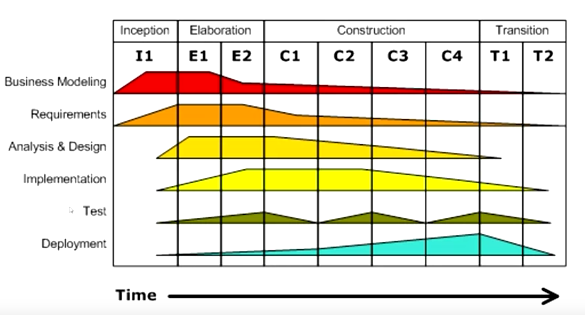
\includegraphics[width=\columnwidth]{imgs/unifiedModel.png}
\end{figure}

Las área de colores indican el nivel de esfuerzo que según este modelo se debe poner en cada una de las fases. Podemos ver que hay cuatro fases: inicio, elaboración, construcción y transición. El inicio está dividido en una sola iteración, la elaboración está dividida en dos iteraciones, y así.\\
El inicio se centra principalmente en el modelado empresarial y los requisitos; por tanto es la fase más corta de todas. EN esta fase se establece el modelo de negocio, también se define el alcance. Luego se hace un estudio de viabilidad para determinar si el proyecto es posible desde el punto de vista del mercado y de la capacidad de ejecución de la companía. Se determina también qué elementos del proyecto serán construidos y cuáles seran comprados. \\
La siguiente es la fase de la elaboración; en esta fase se desarrollan y llevan a cabo muchas actividades en torno a los requisitos. El objetivo clave de esta fase es que se puedan determinar dos objetivos: abordar todos los riesgos conocidos; se hace mucho enfoque en lo que puede salir mal y en cómo puede resolverse. El segundo objetivo es validar la arquitectura del sistema; determinar cómo se va a construir el sistema. Todo esto deriva en una estimación muy creíble para la siguiente fase. \\
Luego viene la fase de construcción. Esta es la fase más grande de todo el proyecto. En esta fase se construye el software mediante múltiples iteraciones, y de cada iteración se produce un lanzamiento; esto quiere ecir que se publica algo en cada iteración y se recibe feedback. 


\section{Elementos especializados de la arquitectura en Python}

\subsection{Proceso en la arquitectura} 

El proceso de diseño de una arquitectura se puede desglosar a tres preocupaciones principales:

\begin{itemize}
    \item Estructura del sistema. Se refiere a cómo el sistema se descompone en estos varios subsistemas principales, y cómo estos se comunican entre sí.
    \item Modelamiento de control. Es la forma en la que la arquitectura realiza un modelo de las relaciones de control entre las diferentes partes del sistema
    \item Descomposición modular. Es la forma en que se identifican las particiones de los subsistemas
\end{itemize}

Otra cosa importante a nivel arquitectónico es cómo podemos evaluar la calidad de un software. Los sisguientes son algunos atributos de calidad que se tienen en cuenta para el Software:

\begin{enumerate}
    \item Modificabilidad
    \item Capacidad de prueba
    \item Escalabilidad y desempeño
    \item Disponibilidad
    \item seguridad
    \item Capacidad de implementación
\end{enumerate}

\subsubsection{Modificabilidad}

Indica la facilidad con la que los cambios pueden ser realizados en el sistema y la flexibilidad con la cual el sistema se ajusta a dichos cambios. Los intereses dentro de la modificabilidad son los siguientes

\begin{itemize}
    \item Dificultad. La facilidad con la que se pueden hacer cambios en el sistema.
    \item Costo. En términos de tiempo y recursos requeridos para hacer los cambios.
    \item Riesgos. Cualquier riesgo asociado con realizar los cambios del sistema.
\end{itemize}

Los tipos de cambios de los que hablamos son cambios en código, cambios de la implementación, cambios incluso de la misma arquitectura. Estos cambios pueden ser a los siguientes niveles:

\begin{enumerate}
    \item Locales. Son cambios sencillos que solamente afectan elementos específicos, Por ejempli una función o método, una clase, un archivo de confguración como un \texttt{\textbf{XML}} o \texttt{\textbf{JSON}}, etc. Esos cambios generalmente no generan un efecto colateral a algún otro elemento cercano. Son los más sencillos de implementar y pueden ser fácolmente validados mediante pruebas unitarias.
    \item No locales. Estos cambios envuelven a más de un elemento. Por ejemplo la modificación de un esquema de base de datos, esto puede llevar a necesitar modificar las abstracciones de las tablas, o los modelos utilizados. Estos cambios ssuelen ser más complicasdos de gestionar y requieren ser validadoos a través de pruebas de integración.
    \item Globales. Pueden ser cambios que estén relacionados directamente con la arquitectura completa, o modificar elementos globales que afectarán a una gran parte de subsistemas. Un ejemplo puede ser el cambio de una aquitectura de RESTful a por ejemplo una arquitectura de mendajes como SOAP. Otro ejemplo puede ser el cambio de framework, pasando de \texttt{\textbf{FastAPI}} a \texttt{\textbf{Flask}}. Estos son los cambios que representan los mayores riesgos y también los mayores costos en términos de tiempo, recursos y dinero.
\end{enumerate}

Los aspectos de cohesión y acoplamiento también determinan una mejor modificabilidad del sistema. Recordemos que la cohesión es el nivel de claridad en la definición de los roles y responsabilidades que tiene un módulo o clase. Y el acoplamiento es el nivel de afectabilidad que puede tener un módulo con otro al ser modificado. Mientras menor sea el acoplamiento y mayor la cohesión, más alta será la modificabilidad.

\subsubsection{Capacidad de prueba} Esta capacidad se refiere a qué tan susceptible a demostrar los fallos mediante pruebas tiene un sistema de software. En otras palabras, se puede referir a una medida de qué tanto el sistema esconde sus fallos a los usuarios finales y a las pruebas de integración. Mientras más testeables es un sistema, menos es capaz de esconder estos errores. También se puede relacional la capacidad de prueba de un sistema con qué tan predecible puede ser su comportamiento. Para recrear la sesión de prueba o el estado en el momento de la falla, a menudo se utiliza una estrategia de record o playback, mediante algún doftware especializado (como Selenium) el cual graba todas las acciones del usuario que llevan a un fallo en particular y las guarda en forma de caso de prueba. La capacidad de prueba también está relacionado con el acoplamiento del código. Mientras menor sea el acoplamiento del código, mayor será la capacidad de prueba del mismo. Otro aspecto importante de esto es la reducción de la aleatoriedad, o el no determinismo. Cuando se escriben bancos de pruebas, es necesario aislar los elementos que se testean de los elementos de su alrededor


\subsubsection{Escalabilidad} Este es un concepto muy importante en los tiempos actuales. En cualquier aplicación de software moderno es muy probable escuchar acerca de trabajar en una aplicación escrita sobre la nube, la cual se puede escalar elásticamente a demanda. La escalabilidad es la capacidad de acomodar o adaptarse al crecimiento de la carga de trabajo en función de la demanda siempre y cuando se mantenga el desempeño dentro de unos límites aceptables. El concepto de escalabilidad siempre se divide en dos categorías principales: 


\paragraph{Escalabilidad horizontal} Este tipo de escalabilidad se refiere a el aumento o adición de nodos computacionales a un sistema de software. Esto ha sido posible gracias a los avances en computación en cluster (lo cual significa el agrupamiento de varios computadores conectados entre sí para trabajar como un solo sistema) en las últimas décadas. Cada uno de estos computadores son denominados ’nodos’ y cada nodo usualmente se trata de servidores virtuales privados. La escalabilidad se logra cuando se añade un nodo adicional, típicamente administrado por un balanceador de cargas. Desescalar es
cuando se eliminan nodos al sistema. 

\paragraph{Escalabilidad vertical} La escalabilidad vertical es cuando se añaden o eliminan más recursos en un solo nodo. Típicamente esto se logra cuando se añaden recursos de hardware como procesadores o memorias RAM.

\subsubsection{Desempeño} El desempeño de un software está relacionado con su escalabilidad. Este puede ser definido de la siguiente forma: el el desempeño de un sistema computacional es la cantidad de trabajo logrado por un sistema utilizando una unidad de recurso de computación dada. A mayor razón trabajo/unidad, mayor será el rendimento. Esta unidad de recurso de computación para medir el desempeño puede ser uno de los siguientes:

\begin{itemize}
    \item Tiempo de respuesta. La cantidad de tiempo que toma una función o cualquier unidad de ejecución en ejecutarse, ya sea en términos de tiempo real o en tiempo de ciclos de reloj.
    \item Latencia. El tiempo que toma un sistema en aceptar una estimulacón y dar una respuesta a esta.
    \item Rendimiento o flujo de procesos. Es la razón a la cual un sistema procesa su información por unidad de tiempo. Un sistema que tiene un mayor desempeño usualmente tendrá un flujo de procesos mayor, y en correcpondencia, una mayor escalabilidad
\end{itemize}

\subsubsection{Disponibilidad} Como su nombre lo indica, es la propiedad de estar listo que tiene un sistema de software para llevar a cabo sus operaciones cuando se necesita. Este atributo de calidad está relacionado de manera directa con la fiabilidad del software. Un factor que también puede modificar la disponibilidad es la habilidad del sistema que tiene para recuperarse de fallos. Hay tres medidas importantes a la hora de manejar los posibles fallos que pueden presentarse en un sistema.

\begin{itemize}
    \item Detección del fallo.
    \item Reuperación del fallo.
    \item Prevención del fallo.
\end{itemize}

Por otra parte, la disponibilidad se puede relacionar con la escalabilidad horizontal de la siguiente forma: Si el sistema es altamente escalable horizontalmente, este tendrá una alta disponibilidad ya que permite al balanceador de carga determinar nodos inactivos y apuntarlos en la configuración rápidamente. Por su parte, la escalabilidad vertical afeca a la disponibilidad teniendo en cuenta que los recursos del nodo no son suficientemente amplios y el programa puede colapsar, disminuyendo así la disponibilidad. 

Con el auge de las aplicaciones web y la computación distribuida, la seguridad de un sistema también se vuelve un factor importante que afecta a la disponibilidad. Si una vulnerabilidad es
explotada por alguna persona maliciosa, el sistema ppuede volverse temporalmente no disponible durante el tiempo en que el ataque esté activo.

\subsubsection{Seguridad} Define el grado de habilidad que tiene un sistema para evitar daños a sus datos y a su lógica de accesos no autorizados, a la vez que continúa proveyendo los servicios a otros sistemas y roles que sí son apropiadamente autorizados y autenticados.

\subsection{Scripting modificable y legible}

En esta sección vamos a adentrarnos de manera profunda en el atributo de modificabilidad y legibilidad. Vamos a dar respuestas claras y completas a las siguientes preguntas:

\begin{itemize}
    \item ¿Qué es la modificabilidad?
    \item Aspectos relacionados a la modificabilidad
    \item Entendimiento de la legibilidad
    \item Fundamentos de la modificabilidad - cohesión y acoplamiento
    \item Exploración de estrategias para conseguir modificabilidad
    \item Métricas - herramientas para el análisis de estadísticas
    \item Refactorización de código
\end{itemize}

\subsubsection{¿Qué es la modificabilidad?} La definición de modificabilidad es la siguiente: Modificabilidad se define como el grado de facilidad con la que se pueden hacer cambios en un sistema y la flexibilidad con la que el sistema se adapta a dichos cambios.

\subsubsection{Aspectos relacionados con la modificabilidad} Hay muchos aspectos que están estrechamente relacionados con la modificabilidad. Entre ellos los siguientes atributos de calidad:


\paragraph{Legibilidad} Se define como la facilidad con la que la lógica de un programa puede ser seguido y entendido. Un software legible contiene un código que ha sido escrito de una manera específica, siguiendo unos parámetros que son típicamente adoptados por el lenguaje de programación y cuya lógica utiliza las características proveídas por el  lenguaje en una manera clara y concisa.

\paragraph{Modularidad} Significa que el código está escrito en módulos bien encapsulados, los cuales desarrollan funciones bien documentadas y específicas. En otras palabras, un cósigo modular provee al programador APIs amigables al resto del sistema. 

\paragraph{Reusabilidad} Es una medida del número de partes del software, ya sea código, herramientas, diseños, y demás, que pueden ser reutilizados en otras partes del sistema con nula o muy poca modificación. Un buen diseño debería enfatizar en la reusabiidad desde el principio. 

\paragraph{Manteniblidad} Se define como la facilidad y eficiencia con la que el sistema puede ser actualizado y mantenerse trabajando de una manera efectiva para sus personas interesadas.

\subsubsection{Entendimiento de la legibilidad} Un códico que esté bien escrito y documentado, manteniendo los estándares y adoptando buenas prácticas en función del lenguaje de programación, tenderá a producir código simple y conciso que será fácil de leer y de modificar. No solamente está relacionado con buenas prácticas de escritura de código, sino también en la claridad misma de la lógica de los algoritmos, la modularidad, ydemás aspectos. Podemos resumir los aspectos de la siguiente manera:


\begin{itemize}
    \item Bien escrito. Se considera si el código contiene una sintaxis simple, una lógica clara y concisa, utilizando nombres para las variables, funciones y clases o módulos con un significado claro y definido, expresando qué es lo que hace.
    \item Bien documentado. Se refiere a los comentarios entre líneas dentro del archivo. Una sección de código bien documentado indica qué es lo que hace, cuáles son las entradas y cuál o cuáles son los valores de retorno si los hay, a lo largo de la lógica del algoritmo, con un cierto nivel de detalle. También se documenta cualquier uso de alguna librería o API externa y la configuración requerida para ejecutar el código.
    \item Bien formateado. En lenguajes como ppython tan ampliamente desarrollados por la comunidad, hay una seria de pautas bien definidas en aspectos tales como estios, identación y formateo.
\end{itemize}

\paragraph{Algunos antipatrones} Aunque python es un lenguaje que facilita la escritura de código legible, no es cierto que todo código que se escriba será siempre legible; se pueden encontrar en la web muchos ejemplos de código difícil de leer que está mal escrito. Algunas de las prácticas que pueden llevar a escritura incorrecta de código, también llamadas antipatrones, son las siguientes:

\begin{enumerate}
    \item Códifgo sin comentarios o con pocos comentarios. Sobre toso porque una documentación siempre ayuda a informar sobre por qué se impementó algún patrón de escritura en particular. Cuando no se escriben comentarios apropiadamente, otros programadores o el mismo programador puede no entender el código o el porqué de ese enfoque.
    \item código que rompe las mejores prácticas de lenguaje. En ocasiones, cuando los programadores son novatos o vienen de otro lenguaje doferente, pueden tener tendencias a escribir código que no se alinea con las práctias que se han venido desarrollando y evolucionando a lo largo de los años por la comunidad de desarrolladores.
    \item Código espagueti. Son las porciones de código que no tienen una estructura discernible o un flujo de control. Genralmente se compone de una lógica extensa y compleja con saltos extraños y manejo de excepciones no estructuradas, etc.
    \item Gran bola de lodo. Estos son programas o módulos con porciones de código que no muestran claramente una estructura u objetivo general. típicamente está hecho de varias piezas espagueti, y usualmente es un signo de código que ha sido escrito por múltiples personas, parcheadas y modificadas varias veces y sin dócumentación. 
    \item Copy-paste. Esto puede producir patrones de código repetitivos y largos, que hacen lo mismo una y otra vez.
    \item Programación con ego. Generalmente cuando un desarrollador experimentado pone su proppio estilo de código, diferente a los patrones recomendados, con florituras que pueden ser difíciles de entender para otras personas.
    \item Indentación mezclada. Esto suele ser especialmente importante cuando se mezclan los espacios con las tabulaciones en las indentaciones. Es importante tenerlo en cuenta.
    \item Mezclas de tipos literales. Las comillas para escribir cadenas de texto ’, " y """ suelen ser a menudo mezcladas y esto dificulta también el entendimiento del código, así como la misma sintaxis.
\end{enumerate}

\paragraph{Técnicas para la legibilidad} Uno de los enfoques que se deben tener en cuenta para mejorar el nivel de legibilidad del código es la documentación apropiada de qué es lo que esta pieza de código hace. La documentación puede verse separada o categorizada de la siguiente forma:

\begin{itemize}
    \item Documentación entre líneas: Estos comentarios están dispuestos dentro del código en sí mismo, y provee documentación acerca de partes de código, funciones, módulos, entre otros.
    \item Documentación externa: Esta es documentación adicional que se encuentra en archivos externos al código y explica cosas como el uso del código, cambios en el mismo, instruccioes de instalación, o despliegue, etc. Como ejemplo tenemos el típico archivo \texttt{\textbf{readme}}.
    \item Manuales de usuario. Estos ya son documentos formales escritos específicamente para personas
    involucradas en particular.
\end{itemize}

El siguiente es un ejemplo de cómo puede verser la documentación en comentarios de una sola línea (con \texttt{\textbf{\#}}):

\begin{VerbatimBold}
# This loop performs a network fetch of the URL, retrying up to 3
# times in case of errors. In case the URL can't be fetched,
# an error is returned.
# Initialize all state
count, ntries, result, error = 0, 3, None, None
while count < ntries:
try:
    # NOTE: We are using an explicit timeout of 30s here
    result = requests.get(url, timeout=30)
except Exception as error:
    print('Caught exception', error, 'trying again after a while')
    # increment count
    count += 1
# sleep 1 second every time
time.sleep(1)
if result == None:
    print("Error, could not fetch URL",url)
    # Return a tuple of (<return code>, <lasterror>)
    return (2, error)
    # Return data of URL
    return result.content
\end{VerbatimBold}


Por otro lado, tenemos la documentación docstring, la cual es una manera simple de explicar qué hace una función mediante una cadena justo después de la declaración de la misma:

\begin{VerbatimBold}
def fetch_url(url, ntries=3, timeout=30):
""" Fetch a given url and return its contents.
@params
    url - The URL to be fetched.
    ntries - The maximum number of retries.
    timeout - Timout per call in seconds.
@returns
    On success - Contents of URL.
    On failure - (error_code, last_error)
"""
# This loop performs a network fetch of the URL,
# retrying up to
# 'ntries' times in case of errors. In case the URL
# can't be fetched, an error is returned.
# Initialize all state
count, result, error = 0, None, None
while count < ntries:
    try:
        result = requests.get(url, timeout=timeout)
    except Exception as error:
        print('Caught exception', error, 'trying again after a while')
        # increment count
        count += 1
        # sleep 1 second every time
        time.sleep(1)
if result == None:
    print("Error, could not fetch URL",url)
    # Return a tuple of (<return code>, <lasterror>)
    return (2, error)
    # Return data of the URL
return result.content
\end{VerbatimBold}

El siguiente es un ejemplo para el docstring de una clase, que tiene una estructura similar a la anterior

\begin{VerbatimBold}
class UrlFetcher(object):
    """ Implements the steps of fetching a URL.
    Main methods:
    fetch - Fetches the URL.
    get - Return the URLs data.
    """
    def __init__(self, url, timeout=30, ntries=3, headers={}):
        """ Initializer.
        @params
            url - URL to fetch.
            timeout - Timeout per connection (seconds).
            ntries - Max number of retries.
            headers - Optional request headers.
        """
        self.url = url
        self.timeout = timeout
        self.ntries = retries
        self.headers = headers
        # Enapsulated result object
        self.result = result
    
    def fetch(self):
        """ Fetch the URL and save the result """
        # This loop performs a network fetch of the URL,
        # retrying
        # up to 'ntries' times in case of errors.
        count, result, error = 0, None, None
        while count < self.ntries:
            try:
                result = requests.get(self.url,
                timeout=self.timeout,
                headers = self.headers)
            except Exception as error:
                print('Caught exception', error, 'trying againafter a while')
                # increment count
                count += 1
                # sleep 1 second every time
                time.sleep(1)
            if result != None:
            # Save result
                self.result = result

    def get(self):
        """ Return the data for the URL """
        if self.result != None:
            return self.result.content
\end{VerbatimBold}

El docstring aqupi describe algunos de los métodos principales de la clase.

Finalmente, los docstring para módulos que recolectan la información a nivel de módulo, principalmente sobre la funcionalidad del módulo y también algún detalle sobre qué hace cada parte del módulo. También puede contener información acerca de dependencias externas específicas.


\begin{VerbatimBold}
"""
urlhelper - Utility classes and functions to work with URLs.
Members:
# UrlFetcher - A class which encapsulates action of
# fetching content of a URL.
# get_web_url - Converts URLs so they can be used on the
# web.
# get_domain - Returns the domain (site) of the URL.
"""

import urllib
import time


def get_domain(url):
    """ Return the domain name (site) for the URL"""
    urlp = urllib.parse.urlparse(url)
    return urlp.netloc

def get_web_url(url, default='http'):
    """ Make a URL useful for fetch requests
    - Prefix network scheme in front of it if not present already
    """
    urlp = urllib.parse.urlparse(url)
    if urlp.scheme == '' and urlp.netloc == '':
        # No scheme, prefix default
        return default + '://' + url
    return url

class UrlFetcher(object):
    """ Implements the steps of fetching a URL.
    Main methods:
    fetch - Fetches the URL.
    get - Return the URLs data.
    """
    def __init__(self, url, timeout=30, ntries=3, headers={}):
        """ Initializer.
        @params
            url - URL to fetch.
            timeout - Timeout per connection (seconds).
            ntries - Max number of retries.
            headers - Optional request headers.
        """ 
        self.url = url
        self.timeout = timeout
        self.ntries = ntries
        self.headers = headers
        # Enapsulated result object
        self.result = result
    def fetch(self):
        """ Fetch the URL and save the result """
        
        # This loop performs a network fetch of the URL, retrying
        # up to 'ntries' times in case of errors.
        count, result, error = 0, None, None
        while count < self.ntries:
            try:
                result = requests.get(self.url,
                timeout=self.timeout,
                headers = self.headers)
            except Exception as error:
                print('Caught exception', error, 'trying againafter a while')
                # increment count
                count += 1
                # sleep 1 second every time
                time.sleep(1)
        if result != None:
            # Save result
            self.result = result
    def get(self):
        """ Return the data for the URL """
        if self.result != None:
            return self.result.content
\end{VerbatimBold}

\paragraph{Seguimiento de pautas de código y estilo} Es común que las empresas tengan sus propias pauas de estilo de código. Para python existe un conjunto bien definido de pautas de elaboración de código para la comunidad de programadores. Estas pautas se llaman PEP-8, se puede encontrar en línea en https://www.python.org/dev/peps/pep-0008/
Estas pautas fueron creadas en 2001 y han sido ampliamente modificadas a lo largo de los años. 

La filosofía de PEP-8 pueden resumirse en los siguientes puntos importantes

\begin{itemize}
    \item Todo código será más leído de lo que será escrito. De manera que con una serie de pautas se puede conseguir un código más legible y hacerlo consistente a lo largo de un espectro total de código.
    \item La consistencia dentro de un proyecto es importante. Sin embargo, la consistencia dentro de un paquete o módulo es aún más importante. Y la consistencia dentro de una unidad de código tales una clase o función es lo más importante.
    \item Es importante saber en qué momento ignorar una pauta. Por ejemplo si dicha pauta puede hacer que el código sea más complicado de leer o rompa la compatibilidad con el código al rededor.
    \item Si una pauta no es directamente aplicable o útil para la organización, se puede personalizar. Para cualquier duda es importante saber que se puede pedir ayuda a la comunidad. 
\end{itemize}

\paragraph{Revisión y Refactorización de código} Es importante tener en cuenta que todo código debe tener mantenimientos. Las revisiones periodicas de código es útil para mantener el cógido legible y saludable ayudando a la modificabilidad y la mantenibilidad. 

\paragraph{Comentarios de código} Los comentarios deben ser muy claros y descriptivos; deben explicar lo que hace cada cosa. Algunas pautas que pueden ser útilez a la hora de hacer comentarios son:

\begin{itemize}
    \item Los comentarios en bloque deben estar encima de la lína o líneas que explican. Deben ser claros y concisos, sin redundar ni decir lo obvio.
    \item Los comentarios en líneas (inline) deben evitarse lo máximo posible, solo deben estar si es estrictamente necesario aclarar o explicar por qué esa línea hace lo que hace.
    \item Los comentarios superfluos o que no aporten realmente información deben ser evitados. 
\end{itemize}

\subsubsection{Fundamentos de modificabilidad: cohesión y acoplamiento}

Recordemos las definiciones importantes: kla cohesión se refiere al nivel de cercanía, o qué tan estrechamente relacionadas están las responsabilidades de un módulo con el otro. Un módulo que ejecuta una tarea específica, o un grupo de tareas relacionadas entre sí es uno con alta cohesión. Por otro lado, el acoplamiento se refiere al nivel con el que una unidad de código puede afectar el comportamiento de otra unidad. Si son dos unidades diferentes, estas deberían no tener una estrecha relación, por tanto, el acoplamiento debería ser bajo. 

Por lo anterior, siempre hay que buscar para cualquier programa la mayor cohesión y el menor acoplamiento posible.

\paragraph{Medida para la cohesión y el acoplamiento}

Sea el siguiente código un módulo que implementa funciones que operan con una serie de números.

\begin{VerbatimBold}
""" Module A (a.py) – Provides functions that operate on series of
numbers """

def squares(narray):
    """ Return array of squares of numbers """
    return pow_n(narray, 2)

def cubes(narray):
    """ Return array of cubes of numbers """
    return pow_n(narray, 3)

def pow_n(narray, n):
    """ Return array of numbers raised to arbitrary power n each """
    return [pow(x, n) for x in narray]

def frequency(string, word):
    """ Find the frequency of occurrences of word in string
    as percentage """
    word_l = word.lower()
    string_l = string.lower()
    # Words in string
    words = string_l.split()
    count = w.count(word_l)
    # Return frequency as percentage
    return 100.0*count/len(words)
\end{VerbatimBold}

Por su parte, sea el siguiente módulo B:

\begin{VerbatimBold}
    """ Module B (b.py) – Provides functions implementing some statistical
    methods """
    
    import a
    
    def rms(narray):
        """ Return root mean square of array of numbers"""
        return pow(sum(a.squares(narray)), 0.5)
    
    def mean(array):
        """ Return mean of an array of numbers """
        return 1.0*sum(array)/len(array)
    def variance(array):
        """ Return variance of an array of numbers """
        # Square of variation from mean
        avg = mean(array)
        array_d = [(x – avg) for x in array]
        variance = sum(a.squares(array_d))
        return variance
    def standard_deviation(array):
        """ Return standard deviation of an array of numbers """
        # S.D is square root of variance
        return pow(variance(array), 0.5)
\end{VerbatimBold}

Podemos ver del módulo A que una de las funciones no está relacionada con las demás, dando un nuvel de cohesion más bajo. Por otro lado, el módulo B tiene funciones que dependen directamente de A, como se puede ver \texttt{\textbf{squares}}. Esto idica un acoplamiento grande del módulo B al módulo A. Mientras que el módulo B no tiene ningún acoplamiento con A.

Por su parte, al analizar el acoplamiento de B a A, observamos que la función de dependencia \texttt{\textbf{squares}} es sencilla, aceptando un arreglo y retornando sus raíces. La probabilidad de que hayan cambion en la estructura de esta función es baja, además, no hay un acoplamiento en doble dirección. Por estas razones, el acoplamiento de B a A es un buen acoplamiento y no afecta en la modificabilidad del sistema.

Si dos módulos estuvieran acoplados en ambas direcciones, es decir, que el módulo A importa y utiliza funciones de B, y viceversa, entonces el acoplamiento sería un mal acoplamiento porque cualquier cambio en uno de los módulos puede afectar negativamente y en cascada la dependencia.

\chapter{Pandas}


    En el contexto de la biblioteca `pandas` en Python, un **dataframe** es una estructura de datos bidimensional, similar a una tabla en una base de datos, una hoja de cálculo o una tabla en lenguajes estadísticos como R. Es esencialmente una colección ordenada de columnas, donde cada columna puede tener un tipo de dato diferente (número, cadena, booleano, etc.).

    El término "data tabular" se refiere precisamente a este tipo de datos en forma de tabla, donde:

    \begin{itemize}
        \item Las \textit{filas} representan observaciones o entradas individuales.
        \item Las \textit{columnas} representan características o variables de esas observaciones.
    \end{itemize}

    Matemáticamente, podríamos considerar un dataframe como una matriz \( M \) de dimensiones \( m \times n \), donde \( m \) es el número de filas y \( n \) es el número de columnas. Cada elemento \( M_{ij} \) representa el valor en la i-ésima fila y j-ésima columna.

    Un dataframe en `pandas` proporciona una serie de funcionalidades útiles para manipular y analizar datos tabulares, tales como:

    \begin{enumerate}
        \item Operaciones de filtrado y selección basadas en condiciones.
        \item Agrupaciones y operaciones de agregación.
        \item Fusiones y uniones con otros dataframes.
        \item Operaciones de pivote y reestructuración.
        \item Funcionalidades para manejo de datos faltantes.
        \item  Integración con otras bibliotecas de Python como `numpy`, `scipy` y `matplotlib`.
    \end{enumerate}1.

    Para ilustrar esto con un pequeño ejemplo, considera el siguiente dataframe:

    \[
        \begin{array}{|c|c|c|}
            \hline
            \textbf{Nombre} & \textbf{Edad} & \textbf{Profesión} \\
            \hline
            Juan            & 30            & Ingeniero          \\
            \hline
            Ana             & 25            & Doctora            \\
            \hline
            Carlos          & 28            & Arquitecto         \\
            \hline
        \end{array}
    \]

    En este dataframe:
    Las filas representan a diferentes individuos.
    Las columnas representan características de estos individuos: su nombre, edad y profesión.

    La facilidad con la que `pandas` permite manipular, filtrar y analizar este tipo de datos ha hecho que sea una herramienta esencial para cualquier persona que trabaje con análisis de datos en Python.

    \section{\texttt{Funciones de entradas y salidas}}

        Estas son las funciones mediante las cuales se pueden obtener diferentes objetos de pandas o guardar como salidas.

        \subsection{\texttt{pandas.read\_csv()}}

        Esta función es una de las más utilizadas porque importa directamente un archivo \texttt{csv} y lo convierte en un \texttt{DataFrame} (en la siguiente sección se hablará de este objeto)

            \subsubsection{Parámetros}

                \paragraph{\texttt{filepath\_or\_buffer}}

                    \begin{itemize}
                        \item \textbf{Descripción:} Es la ruta del archivo \textit{csv} a importar. Se puede usar una URL
                        \item \textbf{Tipo:} \texttt{str}. También acepta objetos tipo \texttt{PathLike} u objetos \texttt{path}.
                    \end{itemize}

                \paragraph{\texttt{sep}}

                    \begin{itemize}
                        \item \textbf{Descripción:} El tipo de separador de los datos, normalmente son comas \texttt{','} , pero puede ser configurado según el archivo que se va a importar.
                        \item \textbf{Tipo:} \texttt{str}.
                        \item \textbf{Por defecto:} \textit{','}
                    \end{itemize}

                \paragraph{\texttt{header}}

                    \begin{itemize}
                        \item \textbf{Descripción:} Es la especificación de la fila que contiene las etiquetas de las columnas. Por defecto siempre será la primera.
                        \item \textbf{Tipo:} \texttt{int} , \texttt{infer} o \texttt{None}. Si se especifica \texttt{None}, las etiquetas de las columnas serán índices desde 0 hasta n. Si se especifica \texttt{infer}, se asume que  \texttt{header = 0}
                        \item \textbf{Por defecto:} \textit{infer} .
                    \end{itemize}

                \paragraph{\texttt{index\_col}}

                    \begin{itemize}
                        \item \textbf{Descripción:} Especifica la columna que se usará como etiquetas de las filas.
                        \item \textbf{Tipo:} \texttt{hashable}. Comúnmente suelen ser del tipo numérico (\texttt{int} o \texttt{float}) o cadenas de caracteres \texttt{str}. Básicamente es la etiqueta de la columna que se usará como etiqueta
                        \item \textbf{Por defecto:}  Es opcional.
                    \end{itemize}

                \paragraph{\texttt{usecols}}

                    \begin{itemize}
                        \item \textbf{Descripción:} Se puede seleccionar un conjunto de columnas para importar y descartar las demás. Este parámetro especifica este conjunto
                        \item \textbf{Tipo:} Lista de \texttt{hashables}.
                        \item \textbf{Por defecto:} Es opcional.
                    \end{itemize}



            % \subparagraph{\texttt{}}
            % \begin{itemize}
            %     \item \textbf{Descripción:}
            %     \item \textbf{Tipo:}
            %     \item \textbf{Por defecto:}
            % \end{itemize}

            % \subparagraph{\texttt{}}
            % \subparagraph{\texttt{}}

    \section{Funciones generales}

        \subsection{Filtrado de información}

            Existen varios métodos para filtrar los datos de un \texttt{dataframe}. Los más básicos son los que solamente tienen una condición. También están las múltiples condiciones.

            \subsubsection{Una sola condición:} Si un dataframe con nombre \texttt{df} tiene una columna cuya etiqueta o nombre es \texttt{sex}; una forma de filtrar sería la siguiente:

                \begin{verbatim}
                    df[df.sex == "male"]
                \end{verbatim}

                De esta manera se obtiene o se retorna un dataframe con la información filtrada.

                Por su parte, se puede utilizar el método \texttt{loc} para realizar el filtrado:

                \begin{verbatim}
                    df.loc[df.sex == "male"]    
                \end{verbatim}

                Y si por ejemplo, se quiere solamente se requiere sacar una columna, se usa
                \begin{verbatim}
                    df.loc[df.sex == "male", "fare"]    
                \end{verbatim}

            \subsubsection{Varias condiciones:}


                Una forma de filtrar por el tipo de variable en el dataframe, en este caso se seleccionan una o más columnas

                \begin{verbatim}
                    mask = df.dtypes == "int64"
                    df.loc[mask]    
                \end{verbatim}

                Se pueden definir diferentes máscaras, tanto para las filas como para las columnas.

                \begin{verbatim}
                    mask1 = df["age"] >= 55
                    mask2 = df.dtypes == "int64"
                    df.loc[mask]    
                \end{verbatim}

                Adicionalmente se pueden usar funciones lógicas para mejorar la precisión del filtro:
                \begin{verbatim}
                    df.loc[(df.sex == "male") & (df.age > 25)]    
                \end{verbatim}

                Existen algunas reglas adicionales para máscaras para filtrar de forma más práctica:

                \begin{verbatim}
                    mask = summer["Year"].between(1960, 1984, inclusive = True)
                    mask2 = summer["Year"].isin([1972,1996])
                \end{verbatim}

                Este último es útil para seleccionar explícitamente un conjunto de elementos a filtrar, seleccionándolas o extrayéndolas mediante la negación. El argumento siempre es una lista con los objetos que quiero filtrar.

        \subsection{ELiminación de filas y columnas}

            Existen varias formas de eliminar filas y columnas de los dataframes. La forma más básica es mediante el método \texttt{drop}. Este método tiene el parámetro \texttt{inplace}

            \begin{verbatim}
                df.drop(columns = "col")    
            \end{verbatim}

            Para eliminar más de una columna, se pasa una lista con las etiquetas correspondientes como argumento.


            \begin{verbatim}
                df.drop(columns = ["col1", "col2"])    
            \end{verbatim}

            Dos alternativas para eliminar una columna son las siguientes.

            \begin{verbatim}
                df.drop(labels = "col_name", axis = "columns")
                del df["col"]
            \end{verbatim}

            Para eliminar las filas se utiliza la misma forma, reemplazando \texttt{columns} por \texttt{index}. Con esta forma se eliminan todas las instancias con el índice seleccionado, en caso que haya más de una fila con el mismo índice.

            \begin{verbatim}
                df.drop(index = index_name)
            \end{verbatim}

            Otra forma es renombrando el dataframe con una versión filtrada de la misma

            \begin{verbatim}
                df = df.loc[df.col == value]
            \end{verbatim}

            Aquí se seleccionan solamente las filas cuyo valor para la columna \texttt{col} es \texttt{value}, descartando todas las otras.

            Si creamos diferentes máscaras, y luego filtramos la negación lógica de dichas máscaras, entonces estaremos eliminando las filas que cumplan con la máscara o máscaras.

            \begin{verbatim}
                mask1 = summer["Year"] == 2012
                mask2 = summer["Country"] == "RUS"
                summerf = summer.loc[~(mask1 & mask2)]
            \end{verbatim}


        \subsection{Añadidura de columnas}

            La forma más básica de añadir una nueva columna es asignando un valor constante a dicha columna

            \begin{verbatim}
                df["col_nueva"] = 0
            \end{verbatim}

            Si \texttt{col\_nueva} no existe, entonces se creará y se llenará con el valor 0 para todos los índices. Si la columna ya existe, entonces se reemplazarán todos los valores con la nueva asgnación. Por su parte, si se crea una columna de la siguiente forma

            \begin{verbatim}
                df.new_col = 0
            \end{verbatim}

            En realidad se creará un nuevo atributo para el dataframe, con valor 1, pero no se creará una columna.\\

            Si se utiliza una operación tradicional con una columna del dataframe, se creará una columna nueva, y esto se puede utilizar para añadir columnas nuevas con base en datos de otras columnas:

            \begin{verbatim}
                titanic["yob"] = 1912 - titanic["age"]
            \end{verbatim}

            Para añadir una nueva columna en una posición específica, se utiliza el método \texttt{insert}:

            \begin{verbatim}
                col_new = df[col] + 3
                df.insert(loc = 6, column = "new_col_name", value = col_new)
            \end{verbatim}

            De esta forma se asegura que la columna nueva sea localizada en la sexta posición. Las columnas que estén a la derecha serán desplazadas una posición.

            Por otro lado, también se pueden añadir entradas nuevas o filas nuevas. Asignando una lista o iterable concordante con el data frame, a un nuevo índice.



        \subsection{Manupulación de valores}

            Se puede cambiar un solo valor mediante el atributo \texttt{loc} y también \texttt{iloc}

            \begin{verbatim}
                titanic.loc["index","col"] = 40
                titanic.iloc[1,1] = 40
            \end{verbatim}

            \noindent Para cambiar varios valores puede hacerse de la siguiente forma

            \begin{verbatim}
                titanic.loc[1:3, "age"] = 42
            \end{verbatim}

            \noindent Se puede cambiar un rango específico de valores con una lista de valores compatible:

            \begin{verbatim}
                titanic.iloc[1:4, 3] = [43,44,45]
            \end{verbatim}

            \noindent Recordar que con el comando \texttt{loc} si el índice es numérico, se selecciona incluyendo desde el primer número hata el último, mientras que con \texttt{iloc} se seleccionar el índice de forma tradicional como si se tratara de una lista.

            \noindent Para reemplazar o cambiar valores basado en condiciones, se usa la siguiente forma
            \begin{verbatim}
                titanic.loc[titanic.age < 1, "age"]
            \end{verbatim}

            \noindent Por su parte, si se requiere cambiar más de una columna para una entrada (fila) en particular se puede usar el siguiente código

            \begin{verbatim}
                titanic.loc[0,"survived":"age"] = [1, 2, "female", 24.0]
            \end{verbatim}

            \noindent El método \texttt{replace} es útil cuando queremos reemplazar todas las entradas que cumplan una condición

            \begin{verbatim}
                titanic.replace(0, "zero")
            \end{verbatim}

            \noindent Esto reemplaza todos los ceros que haya en la tabla por el texto "zero". \\

            \noindent Es crucial entender que al declarar una variable como referencia a una columna de una tabla, en realidad estamos creando un apuntador a dicha columna. Esto significa que cualquier cambio o reemplazo de valores en esta variable implicará una modificación directa en la columna correspondiente de la tabla:

            \begin{verbatim}
                edad = titanic.age
                edad.loc[1] = 40 # aquí
            \end{verbatim}

            \noindent En el reemplazo de variables dentro de una tala la manera correcta de realizarlo es como se mencionó en la sección anterior, realizarlo de otra forma se considera una mala práctica:

            \begin{verbatim}
                titanic.loc[1,"age"] = 40 # esta es forma correcta
                titanic.age[1] = 40 # esta no se debe relizar
            \end{verbatim}

            \noindent Por otro lado, si se asigna a una variable una o más columnas poniendo una lista como argumento, dicha variable si se modifica, no modificará la tabla original.

            \begin{verbatim}
                sexo = titanic[["sex"]]
                sexo.loc[0] = "ajefemalee"
                sexo.iloc[0] = "ajefemalee" # también aplica para iloc
                titanic # no tendrá el valor modificado
            \end{verbatim}
            
            \noindent Si se utiliza el campo para el índice \texttt{[:]} obtendremos el mismo resultado; sin embargo, al modificar una variable declarada de esta forma, Pandas no generará ninguna advertencia.
            
            \begin{verbatim}
                sexo = titanic.loc[:,["sex"]]}            
            \end{verbatim}
            
            Ahora, si se intenta reemplazar valores mediante la notación de doble paréntesis, como se muestra a continuación
            \begin{verbatim}
                titanic[titanic["age"] < 1]["age"] = 1
            \end{verbatim}
            
            \noindent La tabla no será cambiada, y se mostrará una advertencia. Cuando se ejecuta \texttt{titanic[titanic["age"] < 1]["age"]}, se está realizando dos operaciones de indexación consecutivas. Primero, \texttt{titanic[titanic["age"] < 1]} crea una vista o una copia temporal filtrada del \texttt{DataFrame titanic}, seleccionando solo las filas donde \texttt{age} es menor que 1. Luego, \texttt{["age"]} selecciona la columna \texttt{age} de esta vista o copia temporal. Al intentar asignar un nuevo valor a esta selección, se está modificando la copia temporal y no la tabla original.

            \noindent Pero, si se realiza una selección de la columna primero, y luego se realiza el filtro,
            \begin{verbatim}
                titanic["age"][titanic["age"] < 1] = 1
            \end{verbatim}

            La tabla sí será modificada. Esto es debido a la forma en que se realiza la indexación y asignación en este caso específico. En Pandas, cuando se hace una indexación directa sobre una columna del \texttt{DataFrame}, como en \texttt{titanic["age"]}, se obtiene una vista directa de esa columna en el \texttt{DataFrame} original, no una copia. Esta vista es una referencia a los datos en la columna \texttt{age} dentro del \texttt{DataFrame titanic}. Luego, cuando se aplica un filtro adicional con \texttt{[titanic["age"] < 1]}, se está seleccionando ciertas posiciones de esa vista, y cualquier cambio que hagas aquí se reflejará en el \texttt{DataFrame} original. Al asignar \texttt{= 1} a esta selección, se está modificando directamente los datos en la columna \texttt{age} del \texttt{DataFrame titanic}. Es importante notar que, aunque esta forma de indexación y asignación puede funcionar, no es la recomendada, ya que puede llevar a confusión y a errores sutiles, especialmente en contextos más complejos. \\\

            \noindent En conclusión, es importante tener claridad sobre cuándo se está realizando una vista de un conjunto de datos tomados de una tabla (apuntador a la columna, o conjunto de datos) y cuándo se está realizando una copia (sea temporal o no) de los datos; la copia es un objeto completamente independiente de la tabla original. Si se selecciona una columna mediante la notación de atributo (\texttt{titanic.age}) o mediante la notación de paréntesis cuadrados, o cualquier otra notación, es fácil y muy útil utilizar el atributo \texttt{\_is\_view} y el método \texttt{\_is\_copy()}.

            \subsubsection{Consejos de buena práctica:} 
                En general, según el propósito que se tenga, es conveniente y recomendado utilizar cierto tipo de métodos y atributos a la hora de manipular datos de una tabla.
                Si se requiere trabajar y manipular la tabla entera, entones el consejo es evitar el indexado encadenado. La indexación encadenada en Pandas se refiere al proceso de realizar varias operaciones de indexación sucesivas, una tras otra, típicamente utilizando corchetes \texttt{[]}. Esto suele verse en la forma de \texttt{dataframe[...][...]}, donde se realizan dos (o más) operaciones de indexación de forma secuencial. Por su parte, si se desea trabajar con porciones de la tabla, es recomendado realizar una copia de dicha porción mediante el método \texttt{copy()} y trabajar sobre esta.

        \subsection{Métodos de ordenamiento}

            \noindent La manera clásica de ordenar una tabla basado en una columna es la siguiente
            \begin{verbatim}
                titanic.sort_values(by = "age")
            \end{verbatim}
            Recordar que la línea anterior retorna la tabla ordenada, no modifica la actual, para hacer esto se debe usar el parámetro \texttt{inplace}. Recordar también el parámetro \texttt{ascending}.

            \noindent Se puede hacer ordenamiento no solamente por una columna sino por varias, pasando la lista con las etiquetas de las columnas como argumento del parámetro \texttt{by}. La columna de la primera etiqueta de la lista que se pasa como argumento es la que tiene la primera prioridad. También se puede pasar una lista booleana especificando cuáles se ordenarán de forma ascendente y cuáles descendente.
            \begin{verbatim}
                titanic.sort_values(by = ["col1", "col2", "col3"], ascending = [True False False], inplace = True)
            \end{verbatim}
            \noindent Siempre se puede reordenar la tabla con base en el índice de las filas:
            \begin{verbatim}
                titanic.sort_index(ascending = True, inplace = True)
            \end{verbatim}
            Cuando se realiza un ordenamiento basado en una columna, los índices también se ordenan o "desordenan". En algunas ocasionoes se requiere que el índice prevalezca ordenado aun cuando la tabla completa cambió con el ordenamiento. Esto se logra con dos formas distintas:
            \begin{verbatim}
                titanic.sort_values(by = age).reset_index(drop = True)
                titanc.sort_values(by = "age", ignore_index = True)
            \end{verbatim}

        \subsection{Estadísticas con agregación}

            El método \texttt{agg} es utilizado para realizar operaciones de agregación sobre una tabla, permitiendo aplicar una o más funciones sobre sus ejes. Se puede especificar una función, nombre de función, lista de funciones o un diccionario que mapea etiquetas de eje a funciones. Por defecto, estas operaciones se realizan sobre las filas (`axis=0`), pero también pueden aplicarse a las columnas (`axis=1`). El resultado de `agg` puede ser un escalar, una Serie o un DataFrame, dependiendo de la operación. Una forma efectiva de usarlo es seleccionar columnas de un tipo específico, como las numéricas, y luego aplicar un diccionario para realizar distintas operaciones en cada columna, tal como \texttt{df.select\_dtypes("number").agg({"col1": "mean", "col2": ["min", "std"]})}. Esto permite realizar análisis detallados y personalizados sobre los datos de manera eficiente.

        \subsection{Uso de funciones definidas en las tablas}

            \noindent Una funcionalidad interesante es la posibilidad de ejecutar funciones sobre todos los elementos de una tabla. Si definimos una función
            \begin{verbatim}
                def range(series):
                    return series.max() - series.min()
            \end{verbatim}
            \noindent Al implementar el método \texttt{apply} se puede ejecutar la función para los elementos de la columna o los elementos de las filas, según se establezca:
            \begin{verbatim}
                sales.apply(range, axis = 0)
            \end{verbatim}
            El valor de \texttt{axis = 0} es para las filas y \texttt{axis=1} para las columnas. Retornará una tabla con el resultado de la función. \\
            \noindent Se puede pasar la función lambda directamente en caso de requerir poco cóidigo:
            \begin{verbatim}
                sales.apply(lambda x: x.max() - x.min(), axis = 0)
            \end{verbatim}
            Si se selecciona una sola columna o porción de ella, el intérprete ya sabe que se ejecutará la función a dichos elementos:
            \begin{verbatim}
                sales.loc[1:10,"col1"].apply(lambda x: x[0])
            \end{verbatim}
            \noindent El método \texttt{map} es similar, con la diferencia de que solamente aplica para series de datos, es decir una columna por ejemplo. Por último, Se puede aplicar una función a toda la tabla (o parte de ella) mediante el siguiente método.
            \begin{verbatim}
                df.applymap(func)
                df.loc[1:99,"col"].applymap(func)
            \end{verbatim}

        \subsection{Multiindexación}
            En una tabla es posible que como índice, no solamente haya una columna, sino más de una:
            \begin{verbatim}
                df.set_index(["col1", "col2 "])
            \end{verbatim}
            Podemos ordenar de forma personalizada los diferentes índices:
            \begin{verbatim}
                df.sort__index(ascending = [True False])
            \end{verbatim}
            Como podemos ver, hay un índices exterior y uno interior, este orden puede ser cambiado mediante el método:
            \begin{verbatim}
                df.swaplevel()
            \end{verbatim}
            Se puede restablecer el índice de la siguiente forma:
            \begin{verbatim}
                df.reset_index(inplace = True)
            \end{verbatim}
            El indexador \texttt{loc} puede ser usado de la siguiente manera para poder extraer o filtrar información necesaria de una tabla:
            si se desea filtrar ambos índices y luego ver una columna, los índices deben ser puestos en una tupla:
            \begin{verbatim}
                df.loc[(idx1,idx2), col]
            \end{verbatim}
            Se puede no colocar ninguna columna y así veremos todas las columnas.
            Para seleccionar más de un valor para los índices, estos e colocan dentro de una lista. Para extraer todas las columnas, es necesario indicar los dos puntos:
            \begin{verbatim}
                df.loc[([idx1a,idx1b],idx2), col]
                df.loc[([idx1a,idx1b],idx2),:]
            \end{verbatim}
            Para seleccionar todos los valores de un índice, la notación \texttt{:} poroduce un error, por tanto se debe usar \texttt{slice(None)}:
            \begin{verbatim}
                df.loc[([idx1a,idx1b],slice(None)),:]
            \end{verbatim}

            \subsubsection{Operaciones con cadenas de texto}
                Para todos los datos dentro de una tabla que sean cadenas de texto, si se requiere realizar cualquier operación, se debe implementar el método \texttt{.str}:
                \begin{verbatim}
                    df.str.lower()
                \end{verbatim}
                Para el método \texttt{split}, se tiene la opción de separar de manera automática el resultado en columnas separadas:
                \begin{verbatim}
                    summer[col].srt.split("," n = 2, expand = True)
                \end{verbatim}
                El parámeto \texttt{n} indica cuántos de los caracteres separadores se requiere tomar, y el parámetro \texttt{expand} indica si se requiere guardar el retorno en columnas separadas. \\
                También es útil utilizar métodos de string como \texttt{contains} para realizar filtros personalizados y especializados:
                \begin{verbatim}
                    summer[summer["Event"].str.contains("100M")]
                \end{verbatim}



    \section{Objeto \texttt{DataFrame}}

        Es una de las clases más importantes de Pandas; una estructura de datos tabular de dos dimensiones. Es una representación en Pandas de una tabla de datos.

        \subsection{Constructor} El constructor es el siguiente

        \begin{verbatim}
                    class pandas.DataFrame(data=None, index=None, columns=None, dtype=None, copy=None)
                    \end{verbatim}
        \subsubsection{Parámetros}

        \paragraph{\texttt{data}}
        \begin{itemize}
            \item \textbf{Descripción:} Es el conjunto de datos que conformará el DataFrame.
            \item \textbf{Tipo:} \texttt{numpy.ndarray}, elementos iterables, \texttt{dict}, o \texttt{DataFrame}
            \item \textbf{Por defecto:} \texttt{None}
        \end{itemize}

        \paragraph{\texttt{index}}
        \begin{itemize}
            \item \textbf{Descripción:} Es el comjunto de etiquetas de las filas de la estructura
            \item     \textbf{Tipo:} \texttt{Index} o arreglo de índices (una lista de \texttt{str}).
            \item     \textbf{Por defecto:} \texttt{None}
        \end{itemize}

        \paragraph{\texttt{columns}}
        \begin{itemize}
            \item \textbf{Descripción:} Es el conjunto de etiquetas de las columnas de la estructura
            \item \textbf{Tipo:} \texttt{Index} o arreglo de índices (lista de \texttt{str}).
            \item \textbf{Por defecto:} \texttt{None}.
        \end{itemize}

        \subsection{Atributos}

        La siguiente es la lista de los atributos de la clase \texttt{DataFrame}

        \subsubsection{~\hspace{2em} \texttt{T}:} La transposición del DataFrame.

        \subsubsection{~\hspace{2em}\texttt{at}:} Accede a un valor único para un par etiqueta de fila/columna.

        \subsubsection{~\hspace{2em}\texttt{attrs}:} Diccionario de atributos globales de este conjunto de datos.

        \subsubsection{~\hspace{2em}\texttt{axes}:} Devuelve una lista que representa los ejes del DataFrame (lista de \texttt{Index}).

        \subsubsection{~\hspace{2em}\texttt{columns[]}:} Las etiquetas de columna del DataFrame. Pueden indexarse como una lista.

        \subsubsection{~\hspace{2em}\texttt{dtypes}:} Devuelve los tipos de datos en el DataFrame.

        \subsubsection{~\hspace{2em}\texttt{empty}:} Indicador de si la Serie/DataFrame está vacío.

        \subsubsection{~\hspace{2em}\texttt{flags}:} Obtiene las propiedades asociadas con este objeto pandas.

        \subsubsection{~\hspace{2em}\texttt{iat}:} Accede a un valor único para un par fila/columna por posición entera.

        \subsubsection{~\hspace{2em}\texttt{iloc}:} Indexación basada puramente en la ubicación por posición entera.

        \subsubsection{~\hspace{2em}\texttt{index[]}:} El índice (etiquetas de fila) del DataFrame. Puede indexarse como en una lista.

        \subsubsection{~\hspace{2em}\texttt{loc}:} Accede a un grupo de filas y columnas por etiqueta(s) o un array booleano.

        \subsubsection{~\hspace{2em}\texttt{ndim}:} Devuelve un entero que representa el número de ejes / dimensiones del array.

        \subsubsection{~\hspace{2em}\texttt{shape}:} Devuelve una tupla que representa la dimensionalidad del DataFrame.

        \subsubsection{~\hspace{2em}\texttt{size}:} Devuelve un entero que representa el número de elementos en este objeto.

        \subsubsection{~\hspace{2em}\texttt{style}:} Devuelve un objeto Styler.

        \subsubsection{~\hspace{2em}\texttt{values}:} Devuelve una representación en Numpy del DataFrame.


        \begin{enumerate}
            \item\texttt{pd.options.display.min\_rows}
            \item\texttt{pd.options.display.max\_rows}
        \end{enumerate}
        Estas variables se modifican a conveniencia para mostrar una cantidad mínima y máxima requerida de los datos de la tabla.

        \subsection{Métodos}
        % \paragraph{\texttt{method1}} descripción
        % \subparagraph{\textbf{parámetros}}
        %     \begin{itemize}
        %         \item \texttt{param1}
        %             \begin{itemize}
        %                 \item \textbf{Descripción:}
        %                 \item \textbf{Tipo:}
        %                 \item \textbf{Por defecto:}
        %             \end{itemize}
        %     \end{itemize}

        % \subparagraph{\textbf{Tipo de retorno:}}

        \subsubsection{\texttt{abs()}} Devuelve una Serie/DataFrame con el valor numérico absoluto de cada elemento.
        \paragraph{\textbf{parámetros}}
        \begin{itemize}
            \item \texttt{Ninguno}
        \end{itemize}
        \subparagraph{\textbf{Retorno:}} \texttt{pandas.Series} o \texttt{Pandas.DataaFrame}

        \subsubsection{\texttt{add(other, axis, level, fill\_value)}} Obtiene la suma de los elementos (elemento a elemento) del dataframe con otro dataframe (u objeto similar).
        \paragraph{\textbf{parámetros}}
        \begin{itemize}
            \item \texttt{other}
                \begin{itemize}
                    \item \textbf{Descripción:} Objeto con el cual se realiza la suma.
                    \item \textbf{Tipo:} \texttt{Serie}, \texttt{DataFrame}, \texttt{dict} o cualquier escalar o secuencia.
                    \item \textbf{Por defecto:} Ninguno
                \end{itemize}
            \item \texttt{axis}
                \begin{itemize}
                    \item \textbf{Descripción:} Selecciona si comparar por el índice o por la columna.
                    \item \textbf{Tipo:} \texttt{0} o \texttt{'index'}, \texttt{1} o \texttt{'column'}
                    \item \textbf{Por defecto:} \texttt{'columns'}
                \end{itemize}
            \item \texttt{fill\_value}
                \begin{itemize}
                    \item \textbf{Descripción:} Rellenar valores que potencialmente serán no determinados (\texttt{NaN}). Esto es especialmente útil cuando se usan dos tablas con diferentes índices y/o columnas.
                    \item \textbf{Tipo:} \texttt{float} o \texttt{None}
                    \item \textbf{Por defecto:} \texttt{None}
                \end{itemize}
        \end{itemize}
        \paragraph{Retorno:} \texttt{DataFrame} con los resultados de los valores





        \subsubsection{\texttt{add\_prefix(prefix, axis)}} Añade un prefijo a las columnas. Si la columna es \texttt{'a'} y el prefijo dado es \texttt{'col\_'}, la columna queda etiquetada como \texttt{col\_a}. No modifica el objeto (retorna uno nuevo)
        \paragraph{\textbf{parámetros}}
        \begin{itemize}
            \item \texttt{prefix}
                \begin{itemize}
                    \item \textbf{Descripción:} La cadena de texto para prefijar.
                    \item \textbf{Tipo:} \texttt{String}
                    \item \textbf{Por defecto:} Ninguno
                \end{itemize}
            \item \texttt{axis}
                \begin{itemize}
                    \item \textbf{Descripción:} Selecciona el eje al cual añadir el prefijo.
                    \item \textbf{Tipo:}  \texttt{0} o \texttt{'index'}, \texttt{1} o \texttt{'column'}
                    \item \textbf{Por defecto:} \texttt{None}
                \end{itemize}
        \end{itemize}
        \paragraph{Retorno:} \texttt{DataFrame}


        \subsubsection{\texttt{add\_suffix(suffix, axis)}} Añade un sufijo a las columnas. Análogo al método anterior.
        \paragraph{\textbf{parámetros}}
        \begin{itemize}
            \item \texttt{suffix}
                \begin{itemize}
                    \item \textbf{Descripción:} La cadena de texto a añadir.
                    \item \textbf{Tipo:} \texttt{String}
                    \item \textbf{Por defecto:} Ninguno
                \end{itemize}
            \item \texttt{axis}
                \begin{itemize}
                    \item \textbf{Descripción:} Selecciona el eje al cual añadir el sufijo.
                    \item \textbf{Tipo:} \texttt{0} o \texttt{'index'}, \texttt{1} o \texttt{'column'}
                    \item \textbf{Por defecto:} \texttt{None}
                \end{itemize}
        \end{itemize}
        \paragraph{Retorno:} \texttt{DataFrame}


        \subsubsection{\texttt{agg(func, axis)}} Agrega utilizando una o más operaciones sobre el eje especificado.
        \paragraph{\textbf{parámetros}}
        \begin{itemize}
            \item \texttt{func}
                \begin{itemize}
                    \item \textbf{Descripción:} La función o funciones para aplicar.
                    \item \textbf{Tipo:} Función o lista de funciones (como ejemplo \texttt{'sum'})
                    \item \textbf{Por defecto:} Ninguno
                \end{itemize}
            \item \texttt{axis}
                \begin{itemize}
                    \item \textbf{Descripción:} Eje sobre la cual realizar la función, si esta última está definida para listas.
                    \item \textbf{Tipo:} \texttt{0} o \texttt{'index'}, \texttt{1} o \texttt{'column'}
                    \item \textbf{Por defecto:} \texttt{0}
                \end{itemize}
        \end{itemize}
        \paragraph{Retorno:} \texttt{DataFrame}, \texttt{Series} o puede ser escalar, dependiendo de la función usada.


        \subsubsection{\texttt{align(other, join, axis, level, copy, fill\_value)}}
        Alinea dos objetos en sus ejes con el método de unión especificado. El método de unión está especificado para cada índice de eje.

        \paragraph{\textbf{Parámetros}}
        \begin{itemize}
            \item \texttt{other}
                \begin{itemize}
                    \item \textbf{Descripción:} DataFrame o Series con el que se quiere alinear.
                    \item \textbf{Tipo:} DataFrame o Series
                    \item \textbf{Por defecto:} Ninguno
                \end{itemize}
            \item \texttt{join}
                \begin{itemize}
                    \item \textbf{Descripción:} Tipo de alineación a realizar (\texttt{'outer'}, \texttt{'inner'}, \texttt{'left'}, \texttt{'right'}).
                    \item \textbf{Tipo:} Cadena de texto
                    \item \textbf{Por defecto:} \texttt{'outer'}
                \end{itemize}
            \item \texttt{axis}
                \begin{itemize}
                    \item \textbf{Descripción:} Eje permitido del otro objeto.
                    \item \textbf{Tipo:} \texttt{0}, \texttt{1}, o \texttt{None}
                    \item \textbf{Por defecto:} \texttt{None}
                \end{itemize}
            \item \texttt{level}
                \begin{itemize}
                    \item \textbf{Descripción:} Difunde a través de un nivel, coincidiendo con los valores del índice en el nivel MultiIndex pasado.
                    \item \textbf{Tipo:} Entero o nombre de nivel
                    \item \textbf{Por defecto:} \texttt{None}
                \end{itemize}
            \item \texttt{copy}
                \begin{itemize}
                    \item \textbf{Descripción:} Siempre devuelve nuevos objetos. Si \texttt{copy=False} y no se requiere reindexación, se devuelven los objetos originales.
                    \item \textbf{Tipo:} Booleano
                    \item \textbf{Por defecto:} \texttt{True}
                \end{itemize}
            \item \texttt{fill\_value}
                \begin{itemize}
                    \item \textbf{Descripción:} Valor a utilizar para valores faltantes. Por defecto es NaN, pero puede ser cualquier valor "compatible".
                    \item \textbf{Tipo:} Escalar
                    \item \textbf{Por defecto:} \texttt{np.nan}
                \end{itemize}
        \end{itemize}

        \paragraph{Retorno:} Tupla de (Series/DataFrame, tipo del otro objeto)
        \begin{itemize}
            \item \textbf{Descripción:} Objetos alineados.
            \item \textbf{Tipo:} Tupla
        \end{itemize}


        \subsubsection{\texttt{all(axis, bool\_only, skipna, **kwargs)}}
        Devuelve si todos los elementos son \texttt{True}, potencialmente a lo largo de un eje. Devuelve \texttt{True} a menos que haya al menos un elemento dentro de una serie o a lo largo de un eje de DataFrame que sea \texttt{False} o equivalente (p. ej., cero o vacío).

        \paragraph{\textbf{Parámetros}}
        \begin{itemize}
            \item \texttt{axis}
                \begin{itemize}
                    \item \textbf{Descripción:} Indica qué eje o ejes deben reducirse. Para Series, este parámetro no se utiliza y se establece en 0 por defecto.
                    \item \textbf{Tipo:} \texttt{0} o \texttt{'index'}, \texttt{1} o \texttt{'columns'}, \texttt{None}
                    \item \textbf{Por defecto:} \texttt{0}
                \end{itemize}
            \item \texttt{bool\_only}
                \begin{itemize}
                    \item \textbf{Descripción:} Incluye solo columnas booleanas. No implementado para Series.
                    \item \textbf{Tipo:} Booleano
                    \item \textbf{Por defecto:} \texttt{False}
                \end{itemize}
            \item \texttt{skipna}
                \begin{itemize}
                    \item \textbf{Descripción:} Excluye valores NA/nulos. Si toda la fila/columna es NA y \texttt{skipna} es \texttt{True}, entonces el resultado será \texttt{True}, como en el caso de una fila/columna vacía. Si \texttt{skipna} es \texttt{False}, entonces los NA se tratan como \texttt{True}, porque no son iguales a cero.
                    \item \textbf{Tipo:} Booleano
                    \item \textbf{Por defecto:} \texttt{True}
                \end{itemize}
            \item \texttt{**kwargs}
                \begin{itemize}
                    \item \textbf{Descripción:} Palabras clave adicionales no tienen efecto pero podrían ser aceptadas para compatibilidad con NumPy.
                    \item \textbf{Tipo:} Cualquiera
                    \item \textbf{Por defecto:} \texttt{None}
                \end{itemize}
        \end{itemize}

        \paragraph{Retorno:} Series o DataFrame
        \begin{itemize}
            \item \textbf{Descripción:} Si se especifica un nivel, se devuelve un DataFrame; de lo contrario, se devuelve una Series.
            \item \textbf{Tipo:} Series o DataFrame
        \end{itemize}



        \subsubsection{\texttt{DataFrame.any(*, axis=0, bool\_only=False, skipna=True, **kwargs)}}
        Devuelve si algún elemento es \texttt{True}, potencialmente a lo largo de un eje. Devuelve \texttt{False} a menos que haya al menos un elemento dentro de una serie o a lo largo de un eje de DataFrame que sea \texttt{True} o equivalente (p.ej., no cero o no vacío).

        \paragraph{\textbf{Parámetros}}
        \begin{itemize}
            \item \texttt{axis}
                \begin{itemize}
                    \item \textbf{Descripción:} Indica qué eje o ejes deben reducirse. Para Series, este parámetro no se utiliza y se establece en 0 por defecto.
                    \item \textbf{Tipo:} \texttt{0} o \texttt{'index'}, \texttt{1} o \texttt{'columns'}, \texttt{None}
                    \item \textbf{Por defecto:} \texttt{0}
                \end{itemize}
            \item \texttt{bool\_only}
                \begin{itemize}
                    \item \textbf{Descripción:} Incluye solo columnas booleanas. No implementado para Series.
                    \item \textbf{Tipo:} Booleano
                    \item \textbf{Por defecto:} \texttt{False}
                \end{itemize}
            \item \texttt{skipna}
                \begin{itemize}
                    \item \textbf{Descripción:} Excluye valores NA/nulos. Si toda la fila/columna es NA y \texttt{skipna} es \texttt{True}, entonces el resultado será \texttt{False}, como en el caso de una fila/columna vacía. Si \texttt{skipna} es \texttt{False}, entonces los NA se tratan como \texttt{True}, porque no son iguales a cero.
                    \item \textbf{Tipo:} Booleano
                    \item \textbf{Por defecto:} \texttt{True}
                \end{itemize}
            \item \texttt{**kwargs}
                \begin{itemize}
                    \item \textbf{Descripción:} Palabras clave adicionales no tienen efecto pero podrían ser aceptadas para compatibilidad con NumPy.
                    \item \textbf{Tipo:} Cualquiera
                    \item \textbf{Por defecto:} \texttt{None}
                \end{itemize}
        \end{itemize}

        \paragraph{Retorno:} Series o DataFrame
        \begin{itemize}
            \item \textbf{Descripción:} Si se especifica un nivel, se devuelve un DataFrame; de lo contrario, se devuelve una Series.
            \item \textbf{Tipo:} Series o DataFrame
        \end{itemize}






        \subsubsection{\texttt{head(n)}} Esta función retorna las primeras \( n \) filas del objeto basado en su posición. Es útil para comprobar rápidamente si el objeto contiene el tipo correcto de datos.

        Para valores negativos de \( n \), esta función devuelve todas las filas excepto las últimas \( |n| \) filas, equivalente a \( \text{df}[:n] \).

        Si \( n \) es mayor que el número de filas, esta función retorna todas las filas.

        \paragraph{\textbf{Parámetros}}
        \begin{itemize}
            \item \texttt{n}
                \begin{itemize}
                    \item \textbf{Descripción:} Número de filas a seleccionar.
                    \item \textbf{Tipo:} Entero
                    \item \textbf{Por defecto:} 5
                \end{itemize}
        \end{itemize}

        \paragraph{Retorno:} Mismo tipo que el objeto que llama
        \begin{itemize}
            \item \textbf{Descripción:} Las primeras \( n \) filas del objeto que llama la función.
            \item \textbf{Tipo:} Mismo tipo que el objeto que llama
        \end{itemize}


        \paragraph{Tipo de dato de salida} \texttt{DataFrame}

        \subsubsection{\texttt{tail(n=5)}} Esta función retorna las últimas \( n \) filas del objeto basado en su posición. Es útil para verificar rápidamente los datos, por ejemplo, después de ordenar o agregar filas.

        Para valores negativos de \( n \), esta función devuelve todas las filas excepto las primeras \( |n| \) filas, equivalente a \( \text{df}[|n|:] \).

        Si \( n \) es mayor que el número de filas, esta función retorna todas las filas.

        \paragraph{\textbf{Parámetros}}
        \begin{itemize}
            \item \texttt{n}
                \begin{itemize}
                    \item \textbf{Descripción:} Número de filas a seleccionar.
                    \item \textbf{Tipo:} Entero
                    \item \textbf{Por defecto:} 5
                \end{itemize}
        \end{itemize}

        \paragraph{Retorno:} Tipo del objeto que llama la función
        \begin{itemize}
            \item \textbf{Descripción:} Las últimas \( n \) filas del objeto que llama la función.
            \item \textbf{Tipo:} Tipo del objeto que llama la función
        \end{itemize}



        \subsubsection{\texttt{info(verbose, buf, max\_cols, memory\_usage, show\_counts)}} Este método imprime información sobre un DataFrame incluyendo el tipo de datos del índice y las columnas, los valores no nulos y el uso de memoria.

        \paragraph{\textbf{Parámetros}}
        \begin{itemize}
            \item \texttt{verbose}
                \begin{itemize}
                    \item \textbf{Descripción:} Si se imprime el resumen completo. Por defecto, se sigue la configuración en \texttt{pandas.options.display.max\_info\_columns}.
                    \item \textbf{Tipo:} Booleano, opcional
                \end{itemize}
            \item \texttt{buf}
                \begin{itemize}
                    \item \textbf{Descripción:} Dónde enviar la salida. Por defecto, la salida se imprime en \texttt{sys.stdout}. Se puede pasar un búfer escribible si se necesita procesar más la salida.
                    \item \textbf{Tipo:} Búfer escribible, valor por defecto \texttt{sys.stdout}
                \end{itemize}
            \item \texttt{max\_cols}
                \begin{itemize}
                    \item \textbf{Descripción:} Cuándo cambiar de la salida detallada a la salida truncada. Si el DataFrame tiene más de \texttt{max\_cols} columnas, se utiliza la salida truncada.
                    \item \textbf{Tipo:} Entero, opcional
                \end{itemize}
            \item \texttt{memory\_usage}
                \begin{itemize}
                    \item \textbf{Descripción:} Especifica si se debe mostrar el uso total de memoria de los elementos del DataFrame (incluido el índice).
                    \item \textbf{Tipo:} Booleano, cadena, opcional
                \end{itemize}
            \item \texttt{show\_counts}
                \begin{itemize}
                    \item \textbf{Descripción:} Si se muestran los recuentos de no nulos. Por defecto, esto se muestra solo si el DataFrame es más pequeño que las opciones en \texttt{pandas.options.display.max\_info\_rows} y \texttt{pandas.options.display.max\_info\_columns}.
                    \item \textbf{Tipo:} Booleano, opcional
                \end{itemize}
        \end{itemize}

        \paragraph{Retorno:} Ninguno
        \begin{itemize}
            \item \textbf{Descripción:} Este método imprime un resumen de un DataFrame y no devuelve nada.
            \item \textbf{Tipo:} Ninguno
        \end{itemize}


        \subsubsection{\texttt{describe(percentiles, include, exclude)}}Genera estadísticas descriptivas. Las estadísticas descriptivas incluyen aquellas que resumen la tendencia central, la dispersión y la forma de la distribución del conjunto de datos, excluyendo los valores NaN. Analiza tanto series numéricas como de objeto, así como conjuntos de columnas de DataFrame de tipos de datos mixtos. La salida variará dependiendo de lo que se proporcione. Consulte las notas a continuación para obtener más detalles.

        \paragraph{\textbf{Parámetros}}
        \begin{itemize}
            \item \texttt{percentiles}
                \begin{itemize}
                    \item \textbf{Descripción:} Los percentiles a incluir en la salida. Todos deben estar entre 0 y 1. El valor por defecto es \([.25, .5, .75]\), que devuelve los percentiles 25, 50 y 75.
                    \item \textbf{Tipo:} Lista de números
                    \item \textbf{Por defecto:} Ninguno (Opcional)
                \end{itemize}
            \item \texttt{include}
                \begin{itemize}
                    \item \textbf{Descripción:} Lista blanca de tipos de datos para incluir en el resultado. Ignorado para Series.
                    \item \textbf{Tipo:} ‘all’, lista de tipos de datos o Ninguno (Por defecto)
                    \item \textbf{Opciones:} ‘all’, lista de dtypes, Ninguno
                \end{itemize}
            \item \texttt{exclude}
                \begin{itemize}
                    \item \textbf{Descripción:} Lista negra de tipos de datos para omitir del resultado. Ignorado para Series.
                    \item \textbf{Tipo:} Lista de tipos de datos o Ninguno (Por defecto)
                    \item \textbf{Opciones:} Lista de dtypes, Ninguno
                \end{itemize}
        \end{itemize}

        \paragraph{Retorno:} Series o DataFrame
        \begin{itemize}
            \item \textbf{Descripción:} Estadísticas resumidas de la Series o DataFrame proporcionado.
            \item \textbf{Tipo:} Series o DataFrame
        \end{itemize}


        \subsubsection{\texttt{len(df)}} Retorna el número de filas que hay en la tabla.
        \subparagraph{Tipo de dato de salida} \texttt{Int}


        \paragraph{\texttt{round(df,0)}} Retorna la tabla con los valores numéricos redondeados con las cifras especificadas.
        \paragraph{Tipo de dato de salida} \texttt{Int}


        \subsubsection{\texttt{mean(axis, skipna, numeric\_only, **kwargs)}} Calcula la media de los valores a lo largo del eje solicitado.

        \paragraph{\textbf{Parámetros}}
        \begin{itemize}
            \item \texttt{axis}
                \begin{itemize}
                    \item \textbf{Descripción:} Eje sobre el que se aplica la función. Para Series, este parámetro no se utiliza y su valor predeterminado es 0. Para DataFrames, especificar \texttt{axis=None} aplicará la agregación en ambos ejes.
                    \item \textbf{Tipo:} \{0 ('index'), 1 ('columns')\}
                    \item \textbf{Por defecto:} \texttt{0}
                \end{itemize}

            \item \texttt{skipna}
                \begin{itemize}
                    \item \textbf{Descripción:} Excluir valores NA/nulos al calcular el resultado.
                    \item \textbf{Tipo:} Booleano
                    \item \textbf{Por defecto:} \texttt{True}
                \end{itemize}

            \item \texttt{numeric\_only}
                \begin{itemize}
                    \item \textbf{Descripción:} Incluir solo columnas de tipo float, int, booleano. No implementado para Series.
                    \item \textbf{Tipo:} Booleano
                    \item \textbf{Por defecto:} \texttt{False}
                \end{itemize}

            \item \texttt{**kwargs}
                \begin{itemize}
                    \item \textbf{Descripción:} Argumentos de palabras clave adicionales para pasar a la función.
                    \item \textbf{Tipo:} Cualquiera
                \end{itemize}
        \end{itemize}

        \paragraph{Retorno:} Series o escalar
        \begin{itemize}
            \item \textbf{Descripción:} La media de los valores a lo largo del eje especificado.
            \item \textbf{Tipo:} \texttt{Series} o escalar
        \end{itemize}




        \subsubsection{\texttt{sort\_values(by, *, axis, ascending, inplace, kind, na\_position, ignore\_index, key)}} Ordena por los valores a lo largo de cualquiera de los ejes.

        \paragraph{\textbf{Parámetros}}
        \begin{itemize}
            \item \texttt{by}
                \begin{itemize}
                    \item \textbf{Descripción:} Nombre o lista de nombres (índices) por los que ordenar.
                    \item \textbf{Tipo:} Cadena de caracteres o lista de cadenas de caracteres, según el índice.
                \end{itemize}

            \item \texttt{axis}
                \begin{itemize}
                    \item \textbf{Descripción:} Eje que será ordenado.
                    \item \textbf{Tipo:} \{0 ('index'), 1 ('columns')\}
                    \item \textbf{Por defecto:} 0
                \end{itemize}

            \item \texttt{ascending}
                \begin{itemize}
                    \item \textbf{Descripción:} Ordenar de forma ascendente vs descendente. Especifique una lista para múltiples órdenes de clasificación.
                    \item \textbf{Tipo:} Booleano o lista de booleanos
                    \item \textbf{Por defecto:} Verdadero
                \end{itemize}

            \item \texttt{inplace}
                \begin{itemize}
                    \item \textbf{Descripción:} Si es Verdadero, aplica el ordenamiento al objeto.
                    \item \textbf{Tipo:} Booleano
                    \item \textbf{Por defecto:} Falso
                \end{itemize}

            \item \texttt{kind}
                \begin{itemize}
                    \item \textbf{Descripción:} Elección del algoritmo de ordenación.
                    \item \textbf{Tipo:} \{'quicksort', 'mergesort', 'heapsort', 'stable'\}
                    \item \textbf{Por defecto:} 'quicksort'
                \end{itemize}

            \item \texttt{na\_position}
                \begin{itemize}
                    \item \textbf{Descripción:} Ubica los NaN al principio si es 'first'; al final si es 'last'.
                    \item \textbf{Tipo:} \{'first', 'last'\}
                    \item \textbf{Por defecto:} 'last'
                \end{itemize}

            \item \texttt{ignore\_index}
                \begin{itemize}
                    \item \textbf{Descripción:} Si es Verdadero, el eje resultante se etiquetará 0, 1, ..., n - 1.
                    \item \textbf{Tipo:} Booleano
                    \item \textbf{Por defecto:} Falso
                \end{itemize}

            \item \texttt{key}
                \begin{itemize}
                    \item \textbf{Descripción:} Aplicar la función clave a los valores antes de ordenar.
                    \item \textbf{Tipo:} Función
                    \item \textbf{Opcional:} Verdadero
                \end{itemize}
        \end{itemize}

        \paragraph{Retorno:} DataFrame o None
        \begin{itemize}
            \item \textbf{Descripción:} DataFrame con valores ordenados o None si \texttt{inplace=True}.
            \item \textbf{Tipo:} DataFrame o None
        \end{itemize}


        \subsubsection{Selección de columnas}

        Si se tiene un DataFrame, podemos usar el índice \texttt{[]} para seleccionar una o más columnas diferentes.

        \begin{verbatim}
                            df["col1"]
                            \end{verbatim}
        Una forma alternativa es mediante la notación de punto:

        \begin{verbatim}
                            df.col1
                            \end{verbatim}
        Si queremos obtener más de una columna, debemos ingresar las etiquetas de dichas columnas como una \textbf{lista}:
        \begin{verbatim}
                            df[["col1","col2"]]
                            \end{verbatim}
        \paragraph{Tipo de dato de salida} Si se pone solamente la etiqueta de una columna como argumento, el tipo de retorno será \texttt{Series}. Si se pone una lista de una o más etiquetas, entonces la salida será otro \texttt{DataFrame}.

        \subsubsection{\texttt{df.iloc[n,m]}} Este método retorna la información de la fila enésima y columna enésima. Se pueden seleccionar una o más filas/columnas, y si se requiere un conjunto específico de filas/columnas, deben ingresarse dentro de una lista
        \begin{verbatim}
                            df.iloc[25:30]
                            df.iloc[25,2]
                            df.iloc[25:30,2:5]
                            df.iloc[[100,345,778],[0,4]]
                            \end{verbatim}
        \paragraph{Tipo de dato de salida} \texttt{Series, DataFrame} o el tipo de objeto en la celda, cuando se especifica una sola celda.

        \subsubsection{\texttt{df.loc[Rlabel,Clabel]}} Este método es muy similar al anterior, con la diferencia de que se asigna como argumento el texto de la etiqueta de la fila que se desea retornar. Si hay más de una fila con la misma etiqueta, entonces se retornan todas las filas.

        \paragraph{Tipo de dato de salida} \texttt{Series, DataFrame} o el tipo de objeto en la celda, cuando se especifica una sola celda.

        Si se intenta capturar los datos de varias filas hasta una etiqueta especificada (por ejemplo, \texttt{df.loc[:"Clabel"]} mostrará error si esta etiqueta no es única.


        En general se puede acceder a las filas o columnas de un conjunto de datos pensando en la entrada de indexación como listas. Si por ejemplo se requiere un rango específico de filas más unas filas específicas, se puede usar lo siguiente

        \begin{verbatim}
                                index = list(range(15,20)) + [35,45]
                                df.iloc[index]
                                \end{verbatim}
        O si se requieren, por ejemplo las tres primeras columnas, más dos columnas específicas más:
        \begin{verbatim}
                                col_index = df.columns[:3].tolist() + ["col7","col9"]
                                df.loc[:, col_index]
                                \end{verbatim}


        \subsubsection{\texttt{copy(deep)}} Realiza una copia de los índices y datos de este objeto.

        \paragraph{\textbf{Descripción}}
        Cuando \texttt{deep=True} (por defecto), se crea un nuevo objeto con una copia de los datos e índices del objeto que hace la llamada. Las modificaciones en los datos o índices de la copia no se reflejarán en el objeto original.

        Cuando \texttt{deep=False}, se crea un nuevo objeto sin copiar los datos o el índice del objeto que hace la llamada (sólo se copian las referencias a los datos y el índice). Cualquier cambio en los datos del original se reflejará en la copia superficial (y viceversa).

        \paragraph{\textbf{Parámetros}}
        \begin{itemize}
            \item \texttt{deep}
                \begin{itemize}
                    \item \textbf{Descripción:} Realizar una copia profunda, incluyendo una copia de los datos y los índices. Con \texttt{deep=False} ni los índices ni los datos se copian.
                    \item \textbf{Tipo:} Booleano
                    \item \textbf{Por defecto:} Verdadero
                \end{itemize}
        \end{itemize}

        \paragraph{\textbf{Retorno:} Series o DataFrame}
        \begin{itemize}
            \item \textbf{Descripción:} El tipo de objeto coincide con el que hace la llamada.
            \item \textbf{Tipo:} Series o DataFrame
        \end{itemize}


        \subsubsection{\texttt{nlargest(n, columns, keep)}} Devuelve las primeras \( n \) filas ordenadas por las columnas en orden descendente.

        \subparagraph{\textbf{Descripción}} Devuelve las primeras \( n \) filas con los valores más grandes en las columnas, en orden descendente. Las columnas que no se especifican también se devuelven, pero no se utilizan para ordenar. Este método es equivalente a \texttt{df.sort\_values(columns, ascending=False).head(n)}, pero es más eficiente en términos de rendimiento.

        \paragraph{\textbf{Parámetros}}
        \begin{itemize}
            \item \texttt{n}
                \begin{itemize}
                    \item \textbf{Descripción:} Número de filas a devolver.
                    \item \textbf{Tipo:} Entero
                \end{itemize}
            \item \texttt{columns}
                \begin{itemize}
                    \item \textbf{Descripción:} Etiqueta(s) de columna por las cuales ordenar.
                    \item \textbf{Tipo:} Etiqueta o lista de etiquetas
                \end{itemize}
            \item \texttt{keep}
                \begin{itemize}
                    \item \textbf{Descripción:} Donde hay valores duplicados:
                            \begin{itemize}
                                \item \texttt{first}: da prioridad a la primera ocurrencia(s).
                                \item \texttt{last}: da prioridad a la última ocurrencia(s).
                                \item \texttt{all}: no elimina ningún duplicado, incluso si eso significa seleccionar más de \( n \) elementos.
                            \end{itemize}
                    \item \textbf{Tipo:} \{`first', `last', `all'\}
                    \item \textbf{Por defecto:} `first'
                \end{itemize}
        \end{itemize}

        \paragraph{\textbf{Retorno:} DataFrame}
        \begin{itemize}
            \item \textbf{Descripción:} Las primeras \( n \) filas ordenadas por las columnas dadas en orden descendente.
            \item \textbf{Tipo:} DataFrame
        \end{itemize}


        \subsubsection{\texttt{nsmallest(n, columns, keep)}} Devuelve las primeras \( n \) filas ordenadas por las columnas en orden ascendente.

        \paragraph{\textbf{Descripción}}
        Devuelve las primeras \( n \) filas con los valores más pequeños en las columnas, en orden ascendente. Las columnas que no se especifican también se devuelven, pero no se utilizan para ordenar.

        Este método es equivalente a \texttt{df.sort\_values(columns, ascending=True).head(n)}, pero es más eficiente en términos de rendimiento.

        \paragraph{\textbf{Parámetros}}
        \begin{itemize}
            \item \texttt{n}
                \begin{itemize}
                    \item \textbf{Descripción:} Número de elementos a recuperar.
                    \item \textbf{Tipo:} Entero
                \end{itemize}
            \item \texttt{columns}
                \begin{itemize}
                    \item \textbf{Descripción:} Nombre o nombres de columna por los cuales ordenar.
                    \item \textbf{Tipo:} Lista o cadena de caracteres
                \end{itemize}
            \item \texttt{keep}
                \begin{itemize}
                    \item \textbf{Descripción:} Si hay valores duplicados:
                            \begin{itemize}
                                \item \texttt{first}: toma la primera ocurrencia.
                                \item \texttt{last}: toma la última ocurrencia.
                                \item \texttt{all}: no elimina ningún duplicado, incluso si eso significa seleccionar más de \( n \) elementos.
                            \end{itemize}
                    \item \textbf{Tipo:} \{`first', `last', `all'\}
                    \item \textbf{Por defecto:} `first'
                \end{itemize}
        \end{itemize}

        \paragraph{\textbf{Retorno:} DataFrame}
        \begin{itemize}
            \item \textbf{Descripción:} Las primeras \( n \) filas ordenadas por las columnas dadas en orden ascendente.
            \item \textbf{Tipo:} DataFrame
        \end{itemize}


        \subsubsection{\texttt{idxmin(axis, skipna, numeric\_only)}} Devuelve el índice de la primera ocurrencia del mínimo a lo largo del eje solicitado. Los valores NA/nulos son excluidos.

        \paragraph{\textbf{Descripción}}
        Esta función retorna el índice de la primera aparición del valor mínimo a lo largo del eje especificado, excluyendo los valores NA/nulos.

        \paragraph{\textbf{Parámetros}}
        \begin{itemize}
            \item \texttt{axis}
                \begin{itemize}
                    \item \textbf{Descripción:} El eje a utilizar. 0 o `index' para filas, 1 o `columns' para columnas.
                    \item \textbf{Tipo:} \{0 o `index', 1 o `columns'\}
                    \item \textbf{Por defecto:} 0
                \end{itemize}
            \item \texttt{skipna}
                \begin{itemize}
                    \item \textbf{Descripción:} Excluir valores NA/nulos. Si una fila/columna entera es NA, el resultado será NA.
                    \item \textbf{Tipo:} Booleano
                    \item \textbf{Por defecto:} Verdadero
                \end{itemize}
            \item \texttt{numeric\_only}
                \begin{itemize}
                    \item \textbf{Descripción:} Incluir solo datos de tipo flotante, entero o booleano.
                    \item \textbf{Tipo:} Booleano
                    \item \textbf{Por defecto:} Falso
                \end{itemize}
        \end{itemize}

        \paragraph{\textbf{Retorno:} Series}
        \begin{itemize}
            \item \textbf{Descripción:} Índices de los mínimos a lo largo del eje especificado.
            \item \textbf{Tipo:} Series
        \end{itemize}

        \paragraph{\textbf{Excepciones}}
        \begin{itemize}
            \item \texttt{ValueError}
                \begin{itemize}
                    \item \textbf{Descripción:} Se levanta si la fila o columna está vacía.
                \end{itemize}
        \end{itemize}

        \paragraph{\texttt{DataFrame.reset\_index}}

        \paragraph{Descripción:}
        Restablece el índice del DataFrame, y utiliza el índice predeterminado en su lugar.
        Si el DataFrame tiene un MultiIndex, este método puede eliminar uno o más niveles.

        \paragraph{Parámetros:}
        \begin{itemize}
            \item \texttt{level}
                \begin{itemize}
                    \item \textbf{Descripción:} Solo elimina los niveles dados del índice. Elimina todos los niveles por defecto.
                    \item \textbf{Tipo:} int, str, tuple, o list
                    \item \textbf{Por defecto:} \texttt{None}
                \end{itemize}

            \item \texttt{drop}
                \begin{itemize}
                    \item \textbf{Descripción:} Si se activa, quita completamente la columna de índices que estaba anteriormente, y la borra.
                    \item \textbf{Tipo:} bool
                    \item \textbf{Por defecto:} \texttt{False}
                \end{itemize}

            \item \texttt{inplace}
                \begin{itemize}
                    \item \textbf{Descripción:} Si se debe modificar el DataFrame en lugar de crear uno nuevo.
                    \item \textbf{Tipo:} bool
                    \item \textbf{Por defecto:} \texttt{False}
                \end{itemize}

            \item \texttt{col\_level}
                \begin{itemize}
                    \item \textbf{Descripción:} Si las columnas tienen múltiples niveles, determina en qué nivel se insertan las etiquetas. Por defecto, se insertan en el primer nivel.
                    \item \textbf{Tipo:} int o str
                    \item \textbf{Por defecto:} \texttt{0}
                \end{itemize}

            \item \texttt{col\_fill}
                \begin{itemize}
                    \item \textbf{Descripción:} Si las columnas tienen múltiples niveles, determina cómo se nombran los otros niveles.
                    \item \textbf{Tipo:} object
                    \item \textbf{Por defecto:} \texttt{''}
                \end{itemize}

            \item \texttt{allow\_duplicates}
                \begin{itemize}
                    \item \textbf{Descripción:} Permite la creación de etiquetas de columna duplicadas.
                    \item \textbf{Tipo:} bool, opcional
                    \item \textbf{Por defecto:} \texttt{lib.no\_default}
                \end{itemize}

            \item \texttt{names}
                \begin{itemize}
                    \item \textbf{Descripción:} Utilizando la cadena dada, renombra la columna del DataFrame que contiene los datos del índice.
                    \item \textbf{Tipo:} int, str o lista 1-dimensional
                    \item \textbf{Por defecto:} \texttt{None}
                \end{itemize}
        \end{itemize}

        \paragraph{Tipo de retorno}
        DataFrame con el nuevo índice o \texttt{None} si \texttt{inplace=True}.


        \subsubsection{\texttt{DataFrame.set\_index}}

        \paragraph{Descripción:}
        Establece el índice del DataFrame utilizando una o más columnas existentes o arrays del mismo tamaño. El índice puede reemplazar el índice existente o expandirse sobre él.

        \paragraph{Parámetros:}
        \begin{itemize}
            \item \texttt{keys}
                \begin{itemize}
                    \item \textbf{Descripción:} Este parámetro puede ser una clave de columna única, un array del mismo tamaño que el DataFrame que llama al método, o una lista que contiene una combinación arbitraria de claves de columna y arrays.
                    \item \textbf{Tipo:} Etiqueta o array-like o lista de etiquetas/arrays
                    \item \textbf{Por defecto:} No aplica
                \end{itemize}

            \item \texttt{drop}
                \begin{itemize}
                    \item \textbf{Descripción:} Elimina las columnas que se utilizarán como el nuevo índice.
                    \item \textbf{Tipo:} bool
                    \item \textbf{Por defecto:} \texttt{True}
                \end{itemize}

            \item \texttt{append}
                \begin{itemize}
                    \item \textbf{Descripción:} Si se deben agregar columnas al índice existente.
                    \item \textbf{Tipo:} bool
                    \item \textbf{Por defecto:} \texttt{False}
                \end{itemize}

            \item \texttt{inplace}
                \begin{itemize}
                    \item \textbf{Descripción:} Si se debe modificar el DataFrame en lugar de crear uno nuevo.
                    \item \textbf{Tipo:} bool
                    \item \textbf{Por defecto:} \texttt{False}
                \end{itemize}

            \item \texttt{verify\_integrity}
                \begin{itemize}
                    \item \textbf{Descripción:} Verifica el nuevo índice en busca de duplicados. De lo contrario, aplaza la verificación hasta que sea necesario.
                    \item \textbf{Tipo:} bool
                    \item \textbf{Por defecto:} \texttt{False}
                \end{itemize}
        \end{itemize}

        \subparagraph{Tipo de retorno}
        DataFrame con las nuevas etiquetas de fila o \texttt{None} si \texttt{inplace=True}.


        \subsubsection{\texttt{DataFrame.rename}}

        \paragraph{Descripción:}
        Renombra las etiquetas de columnas o índices. Los valores de la función o diccionario deben ser únicos (1-a-1). Las etiquetas no contenidas en un diccionario o Serie se mantendrán como están. Las etiquetas adicionales listadas no generarán un error.

        \paragraph{Parámetros:}
        \begin{itemize}
            \item \texttt{mapper}
                \begin{itemize}
                    \item \textbf{Descripción:} Transformaciones dict-like o función para aplicar a los valores del eje especificado.
                    \item \textbf{Tipo:} dict-like o función
                    \item \textbf{Por defecto:} \texttt{None}
                \end{itemize}

            \item \texttt{index}
                \begin{itemize}
                    \item \textbf{Descripción:} Alternativa para especificar el eje.
                    \item \textbf{Tipo:} dict-like o función
                    \item \textbf{Por defecto:} \texttt{None}
                \end{itemize}

            \item \texttt{columns}
                \begin{itemize}
                    \item \textbf{Descripción:} Alternativa para especificar el eje.
                    \item \textbf{Tipo:} dict-like o función
                    \item \textbf{Por defecto:} \texttt{None}
                \end{itemize}

            \item \texttt{axis}
                \begin{itemize}
                    \item \textbf{Descripción:} Eje para aplicar el renombramiento.
                    \item \textbf{Tipo:} \{0 o 'index', 1 o 'columns'\}
                    \item \textbf{Por defecto:} \texttt{0}
                \end{itemize}

            \item \texttt{copy}
                \begin{itemize}
                    \item \textbf{Descripción:} También copia los datos subyacentes.
                    \item \textbf{Tipo:} bool
                    \item \textbf{Por defecto:} \texttt{True}
                \end{itemize}

            \item \texttt{inplace}
                \begin{itemize}
                    \item \textbf{Descripción:} Si se debe modificar el DataFrame en lugar de crear uno nuevo.
                    \item \textbf{Tipo:} bool
                    \item \textbf{Por defecto:} \texttt{False}
                \end{itemize}

            \item \texttt{level}
                \begin{itemize}
                    \item \textbf{Descripción:} En caso de un MultiIndex, solo renombra las etiquetas en el nivel especificado.
                    \item \textbf{Tipo:} int o nombre de nivel
                    \item \textbf{Por defecto:} \texttt{None}
                \end{itemize}

            \item \texttt{errors}
                \begin{itemize}
                    \item \textbf{Descripción:} Si 'raise', genera un KeyError cuando un mapper dict-like, index, o columns contiene etiquetas que no están presentes en el índice que se transforma. Si 'ignore', las claves existentes serán renombradas y las claves adicionales serán ignoradas.
                    \item \textbf{Tipo:} \{'ignore', 'raise'\}
                    \item \textbf{Por defecto:} \texttt{'ignore'}
                \end{itemize}
        \end{itemize}

        \paragraph{Tipo de retorno}
        DataFrame con las etiquetas de eje renombradas o \texttt{None} si \texttt{inplace=True}.




    \section{Objeto \textit{Series}}

    Cuando extraemos una columna entera con sus respectivas filas de un conjunto de datos, el resultado es del tipo \texttt{pandas.core.series.Series}. Este objeto se define dentro del contexto de Pandas como un arreglo unidimensional etiquetado.

    En este objeto hay algunos métodos que son los mismos para los DataFrame

    \begin{itemize}
        \item \texttt{head()}
        \item \texttt{tail()}
        \item \texttt{dtype}
        \item \texttt{shape}
        \item \texttt{index}
    \end{itemize}

    \subsection{Métodos y atributos}

    \subsubsection{\texttt{to\_frame()}} Convierte la serie en un dataframe. Su argumento de entrada. Su único parámetro de entrada es la serie a convertir, y su retorno es un objeto de l tipo DataFrame.

    Existen dos tipos principales de datos en una serie de datos: numéricos y no numéricos. En función del tipo de datos existen diferentes métodos de análisis de las series. Los siguientes son métodos para tipos numéricos.

    \subsubsection{Series.describe()} Este método genera una descripción estadística de los datos.

    \paragraph{Parámetros}

    \begin{itemize}
        \item \textbf{percentiles}:
            \begin{itemize}
                \item \textbf{Tipo}: \texttt{list-like of numbers}
                \item \textbf{Descripción}: Los percentiles a incluir en la salida. Deben estar todos entre 0 y 1.
                \item \textbf{Por defecto}: \texttt{[.25, .5, .75]}
            \end{itemize}

        \item \textbf{include}:
            \begin{itemize}
                \item \textbf{Tipo}: \texttt{'all'}, \texttt{list-like of dtypes} o \texttt{None}
                \item \textbf{Descripción}: Tipo de datos a describir. Si es \texttt{'all'}, se describen todos los tipos.
                \item \textbf{Por defecto}: \texttt{None}
            \end{itemize}

        \item \textbf{exclude}:
            \begin{itemize}
                \item \textbf{Tipo}: \texttt{list-like of dtypes} o \texttt{None}
                \item \textbf{Descripción}: Tipo de datos a excluir de la descripción.
                \item \textbf{Por defecto}: \texttt{None}
            \end{itemize}

        \item \textbf{datetime\_is\_numeric}:
            \begin{itemize}
                \item \textbf{Tipo}: \texttt{bool}
                \item \textbf{Descripción}: Si es \texttt{True}, se tratan las fechas como datos numéricos y se muestra un resumen numérico. Si es \texttt{False}, se muestra un resumen basado en fecha.
                \item \textbf{Por defecto}: \texttt{False}
            \end{itemize}
    \end{itemize}

    \paragraph{Retorno}
    \texttt{Series} o \texttt{DataFrame}
    Con la descripción estadística de la Serie.


    \subsubsection{\texttt{Series.count()}} Cuenta la cantidad de datos no nulos. El tipo de salida es entero.

    \subsubsection{\texttt{Series.sum()}} Retorna la suma de los elementos en la serie de datos. Como característica particular de Pandas, puede manejar de manera apropiada con datos incompletos, o faltantes.

    \paragraph{Parámetros}

    \begin{itemize}
        \item \textbf{axis}:
            \begin{itemize}
                \item \textbf{Tipo}: \texttt{int}
                \item \textbf{Descripción}: El eje a lo largo del cual se aplicará la operación. Para Series, solo se permite el valor 0.
                \item \textbf{Por defecto}: \texttt{0}
            \end{itemize}

        \item \textbf{skipna}:
            \begin{itemize}
                \item \textbf{Tipo}: \texttt{bool}
                \item \textbf{Descripción}: Especifica si se deben excluir los valores \texttt{NaN} al calcular la suma.
                \item \textbf{Por defecto}: \texttt{True}
            \end{itemize}

        \item \textbf{level}:
            \begin{itemize}
                \item \textbf{Tipo}: \texttt{int} o \texttt{str}
                \item \textbf{Descripción}: Si la Serie tiene un MultiIndex, especifica el nivel para calcular la suma.
                \item \textbf{Por defecto}: \texttt{None}
            \end{itemize}

        \item \textbf{min\_count}:
            \begin{itemize}
                \item \textbf{Tipo}: \texttt{int}
                \item \textbf{Descripción}: El número mínimo de observaciones válidas (no-\texttt{NaN}) requeridas para realizar la suma. Si no se alcanza este número, se devuelve \texttt{NaN}.
                \item \textbf{Por defecto}: \texttt{0}
            \end{itemize}
    \end{itemize}

    \textbf{Retorno:}\texttt{scalar} Suma de los valores de la Serie.

    \subsubsection{pandas.Series.mean()} Devuelve la media aritmética de los valores de la Serie.

    \paragraph{Parámetros:}
    \begin{itemize}
        \item \textbf{axis}:
            \begin{itemize}
                \item \textbf{Tipo}: \texttt{int}
                \item \textbf{Por defecto}: \texttt{0}
            \end{itemize}
        \item \textbf{skipna}:
            \begin{itemize}
                \item \textbf{Tipo}: \texttt{bool}
                \item \textbf{Por defecto}: \texttt{True}
            \end{itemize}
    \end{itemize}

    \subsubsection{pandas.Series.median()} Devuelve la mediana de los valores de la Serie.

    \paragraph{Parámetros:}
    \begin{itemize}
        \item \textbf{axis}, \textbf{skipna}, \textbf{numeric\_only}: Igual que en \texttt{Series.mean()}.
    \end{itemize}

    \subsubsection{pandas.Series.std()} Devuelve la desviación estándar de los valores de la Serie.

    \paragraph{Parámetros:}
    \begin{itemize}
        \item \textbf{axis}, \textbf{skipna}, \textbf{level}: Igual que en \texttt{Series.mean()}.
        \item \textbf{ddof}
            \begin{itemize}
                \item \textbf{Tipo}: \texttt{int}
                \item \textbf{Por defecto}: \texttt{1}
                \item \textbf{Desripción}: Delta de los grados de libertad.
            \end{itemize}
    \end{itemize}

    \subsubsection{pandas.Series.min()} Devuelve el valor mínimo de la Serie.

    \paragraph{Parámetros:}
    \begin{itemize}
        \item \textbf{axis}, \textbf{skipna}, \textbf{numeric\_only}: Igual que en \texttt{Series.mean()}.
    \end{itemize}

    \subsubsection{pandas.Series.max()} Devuelve el valor máximo de la Serie.

    \paragraph{Parámetros:}
    \begin{itemize}
        \item \textbf{axis}, \textbf{skipna}, \textbf{numeric\_only}: Igual que en \texttt{Series.mean()}.
    \end{itemize}

    \subsubsection{pandas.Series.unique()} Devuelve los valores únicos de la Serie.

    \paragraph{Parámetros:} Ninguno.

    \paragraph{Tipo de retorno:} \texttt{ExtensionArray}

    \subsubsection{pandas.Series.value\_counts()} Devuelve una Serie que representa la frecuencia de valores únicos.

    \paragraph{Parámetros:}
    \begin{itemize}
        \item \textbf{normalize}:
            \begin{itemize}
                \item \textbf{Tipo}: \texttt{bool}
                \item \textbf{Descripción}: Si es \texttt{True}, devuelve las proporciones en lugar de las cuentas.
                \item \textbf{Por defecto}: \texttt{False}
            \end{itemize}
        \item \textbf{sort}:
            \begin{itemize}
                \item \textbf{Tipo}: \texttt{bool}
                \item \textbf{Por defecto}: \texttt{True}
            \end{itemize}
        \item \textbf{ascending}:
            \begin{itemize}
                \item \textbf{Tipo}: \texttt{bool}
                \item \textbf{Por defecto}: \texttt{False}
            \end{itemize}
        \item \textbf{bins}:
            \begin{itemize}
                \item \textbf{Tipo}: \texttt{int}
                \item \textbf{Descripción}: Solo para Series numéricas. Divide los valores en intervalos.
                \item \textbf{Por defecto}: \texttt{None}
            \end{itemize}
        \item \textbf{dropna}:
            \begin{itemize}
                \item \textbf{Tipo}: \texttt{bool}
                \item \textbf{Descripción}: Si es \texttt{True}, excluye los valores \texttt{NaN}.
                \item \textbf{Por defecto}: \texttt{True}
            \end{itemize}
    \end{itemize}
    \paragraph{Tipo de retorno:} \texttt{Series}

    Para las series con valores no numéricos, los atributos y métodos como \texttt{shape}, \texttt{size}, \texttt{count()} son muy similares a los de valores numéricos. Por su parte otros métodos como \texttt{describe()} muestra información como cuál es el valor más repetido, su respectiva frecuencia, etc.

    Métodos como \texttt{min()} que retorna el valor más "pequeño" alfabéticamente hablando, tienen sus diferencias con los valores numéricos.


    \subsubsection{Ejemplo} Para un conjunto de datos de las medallas de oro de los juegos olímpicos históricos de verano, el siguiente código realiza una exploración de cuál es el nombre del atleta que más oros consiguió en la edición de los juegos olímpicos de 1972:

    \begin{verbatim}
            import pandas as pd
            
            df = pd.read_csv("summer1972.csv",index_col="Year")
            
            Athlete = df["Athlete"]
            
            print(Athlete.loc[1972].value_counts().index[0])
            \end{verbatim}
    \subsection{Creación de series}

    A partir de cualquier conjunto de datos importado o creado, si seleccionamos o extraemos una de las columnas, sea total o filtrada de alguna manera, vamos a obtener un objeto del tipo \textit{Series}.
    La siguiente línea de código es un ejemplo de cómo se consigue una serie directamente importada del archivo:

    \begin{verbatim}
            pd.read_csv("file.csv", usecols = ["name_col"]).squeeze()
            \end{verbatim}
    De este modo, la variable retornada será del tipo \texttt{Series} en lugar de \texttt{DataFrame}.
    Por su parte, existe el método para convertir una lista de python a una serie de pandas:

    \begin{verbatim}
            pd.Series([10,25,6,36,2])
            \end{verbatim}
    Se pueden establecer las etiquetas a las filas de la serie creada de la siguiente forma:
    \begin{verbatim}
            pd.Series([10,25,6,36,2], index = ["Mon","Tue","Wed","Thu","Fri"])
            \end{verbatim}
    Y se puede añadir la etiqueta de la columna también:

    \begin{verbatim}
            pd.Series([10,25,6,36,2], index = ["Mon","Tue","Wed","Thu","Fri"], name = "Sales")
            \end{verbatim}
    \subsubsection{\texttt{pd.Series}} Retorna un objeto del tipo \texttt{Series} a partir de los datos ingresados.

    \paragraph{Parámetros}
    \begin{itemize}
        \item \textbf{data}:
            \begin{itemize}
                \item \textbf{Descripción:} los datos que serán los elementos de la serie.
                \item \textbf{Tipo:} elementos iterables, del tipo arreglo (\texttt{numpy.array}) o diccionarios.
                \item \textbf{Por defecto:} \texttt{None}
            \end{itemize}
        \item \textbf{index}:
            \begin{itemize}
                \item \textbf{Descripción:} Es el conjunto de etiquetas para las filas de la serie.
                \item \textbf{Tipo:} Tipo arreglo, puede ser una lista con los nombres requeridos.
                \item \textbf{Por defecto:} \texttt{None}
            \end{itemize}
        \item \textbf{data}:
            \begin{itemize}
                \item \textbf{Descripción:} los datos que serán los elementos de la serie.
                \item \textbf{Tipo:} elementos iterables, del tipo arreglo (\texttt{numpy.array}) o diccionarios.
                \item \textbf{Por defecto:} \texttt{None}
            \end{itemize}
    \end{itemize}


    \paragraph{Tipo de retorno}: \texttt{Series}


    Por otro lado, se puede crear una variable del tipo \texttt{Series} a partir de arreglos de \textit{numpy}, una lista de python, tupla, o dicccionario:

    \begin{verbatim}
            import pandas as pd
            import numpy as np
            sales = np.array([10,25,6,36,2])
            pd.Series(sales)
            sales = [10,25,6,36,2]
            \end{verbatim}
    Es importante mencionar la diferencia entre las referencias de filas realizadas con \texttt{loc} y las de \texttt{iloc}. Esta última se refiere al \textbf{índice}, iniciando desde cero hasta la longitud menos uno. La primera, \texttt{loc} se refiere a la \textbf{etiqueta}, la cual puede variar.

    \subsubsection{\texttt{sort\_index}}

    \paragraph{Descripción:}
    Ordena la Serie por las etiquetas del índice. Devuelve una nueva Serie ordenada por etiqueta si el argumento \texttt{inplace} es \texttt{False}, de lo contrario, actualiza la Serie original y devuelve \texttt{None}.

    \paragraph{Parámetros:}

    \begin{itemize}
        \item \texttt{axis}
            \begin{itemize}
                \item \textbf{Descripción:} No utilizado. Parámetro necesario para compatibilidad con DataFrame.
                \item \textbf{Tipo:} \{0 o 'index'\}
                \item \textbf{Por defecto:} 0
            \end{itemize}
        \item \texttt{level}
            \begin{itemize}
                \item \textbf{Descripción:} Si no es \texttt{None}, ordena los valores en el nivel de índice especificado.
                \item \textbf{Tipo:} int, opcional
                \item \textbf{Por defecto:} \texttt{None}
            \end{itemize}
        \item \texttt{ascending}
            \begin{itemize}
                \item \textbf{Descripción:} Ordena en dirección ascendente o descendente.
                \item \textbf{Tipo:} bool o lista de bools
                \item \textbf{Por defecto:} \texttt{True}
            \end{itemize}
        \item \texttt{inplace}
            \begin{itemize}
                \item \textbf{Descripción:} Si es \texttt{True}, realiza la operación en el lugar.
                \item \textbf{Tipo:} bool
                \item \textbf{Por defecto:} \texttt{False}
            \end{itemize}
        \item \texttt{kind}
            \begin{itemize}
                \item \textbf{Descripción:} Elección del algoritmo de ordenación.
                \item \textbf{Tipo:} \{'quicksort', 'mergesort', 'heapsort', 'stable'\}
                \item \textbf{Por defecto:} 'quicksort'
            \end{itemize}
        \item \texttt{na\_position}
            \begin{itemize}
                \item \textbf{Descripción:} Posición de los NaNs en la Serie ordenada.
                \item \textbf{Tipo:} \{'first', 'last'\}
                \item \textbf{Por defecto:} 'last'
            \end{itemize}
        \item \texttt{sort\_remaining}
            \begin{itemize}
                \item \textbf{Descripción:} Si es \texttt{True}, también ordena por otros niveles después de ordenar por el nivel especificado.
                \item \textbf{Tipo:} bool
                \item \textbf{Por defecto:} \texttt{True}
            \end{itemize}
        \item \texttt{ignore\_index}
            \begin{itemize}
                \item \textbf{Descripción:} Si es \texttt{True}, el eje resultante se etiquetará de 0 a \( n - 1 \).
                \item \textbf{Tipo:} bool
                \item \textbf{Por defecto:} \texttt{False}
            \end{itemize}
        \item \texttt{key}
            \begin{itemize}
                \item \textbf{Descripción:} Si no es \texttt{None}, aplica la función clave a los valores del índice antes de ordenar.
                \item \textbf{Tipo:} callable, opcional
                \item \textbf{Por defecto:} \texttt{None}
            \end{itemize}
    \end{itemize}

    \paragraph{Tipo de retorno}
    Serie o \texttt{None}. La Serie original ordenada por las etiquetas o \texttt{None} si \texttt{inplace=True}.



    \section{Objeto \texttt{index}}

    Uno de los atributos de un dataframe es \texttt{df.columns}, al imprimir este tipo de objeto vemos que su salida es del tipo

    \begin{verbatim}
            Index(['col1', 'col2', 'col3'], dtype='object')
            \end{verbatim}

    Estas son instancias de la clase \texttt{pandas.index} y se trata de una secuencia inmutable que se utiliza para la indexación y el alineamiento de los datos. Es el objeto en el que se guardan las etiquetas de los ejes en todos los objetos de Pandas.

    \subsection{Métodos}

    \subsubsection{\texttt{Index.append}}

    \paragraph{Descripción:}
    Agrega una colección de opciones de índice juntas.

    \paragraph{Parámetros:}

    \begin{itemize}
        \item \texttt{other}
            \begin{itemize}
                \item \textbf{Descripción:} Índice o lista/tupla de índices a agregar.
                \item \textbf{Tipo:} Index o list/tuple de indices
                \item \textbf{Por defecto:} No aplica
            \end{itemize}
    \end{itemize}

    \paragraph{Tipo de retorno}
    Índice (\texttt{Index}).

    \subsubsection{\texttt{Index.drop}}

    \paragraph{Descripción:}
    Crea un nuevo índice con la lista de etiquetas pasadas eliminadas.

    \paragraph{Parámetros:}

    \begin{itemize}
        \item \texttt{labels}
            \begin{itemize}
                \item \textbf{Descripción:} Etiquetas para eliminar del índice.
                \item \textbf{Tipo:} array-like o escalar
                \item \textbf{Por defecto:} No aplica
            \end{itemize}
        \item \texttt{errors}
            \begin{itemize}
                \item \textbf{Descripción:} Si es 'ignore', suprime el error y se eliminan las etiquetas existentes.
                \item \textbf{Tipo:} \{'ignore', 'raise'\}
                \item \textbf{Por defecto:} 'raise'
            \end{itemize}
    \end{itemize}

    \paragraph{Tipo de retorno}
    Índice (\texttt{Index}). Será del mismo tipo que el índice original, excepto para \texttt{RangeIndex}.

    \paragraph{Excepciones}
    \texttt{KeyError} si no se encuentran todas las etiquetas en el eje seleccionado.



    \paragraph{\texttt{Index.isin}}

    \paragraph{Descripción:}
    Devuelve un array booleano donde los valores del índice están en los valores pasados. Calcula un array booleano que indica si cada valor del índice se encuentra en el conjunto de valores pasado. La longitud del array booleano devuelto coincide con la longitud del índice.

    \paragraph{Parámetros:}

    \begin{itemize}
        \item \texttt{values}
            \begin{itemize}
                \item \textbf{Descripción:} Valores buscados.
                \item \textbf{Tipo:} conjunto o lista
                \item \textbf{Por defecto:} No aplica
            \end{itemize}
        \item \texttt{level}
            \begin{itemize}
                \item \textbf{Descripción:} Nombre o posición del nivel del índice a utilizar (si el índice es un \texttt{MultiIndex}).
                \item \textbf{Tipo:} cadena o entero, opcional
                \item \textbf{Por defecto:} \texttt{None}
            \end{itemize}
    \end{itemize}

    \paragraph{Tipo de retorno}
    Array de NumPy de valores booleanos (\texttt{np.ndarray[bool]}).

    \paragraph{Notas}
    En el caso de \texttt{MultiIndex}, debe especificar los valores como un objeto similar a una lista que contenga tuplas que tengan la misma longitud que el número de niveles, o especificar el nivel. De lo contrario, se generará un \texttt{ValueError}.





    \subsubsection{\texttt{Index.unique}}

    \paragraph{Descripción:}
    Devuelve los valores únicos en el índice. Los valores únicos se devuelven en el orden en que aparecen; esto no ordena los valores.

    \paragraph{Parámetros:}

    \begin{itemize}
        \item \texttt{level}
            \begin{itemize}
                \item \textbf{Descripción:} Devuelve solo los valores del nivel especificado (para \texttt{MultiIndex}). Si es un entero, obtiene el nivel por posición entera; de lo contrario, por nombre del nivel.
                \item \textbf{Tipo:} entero o hashable, opcional
                \item \textbf{Por defecto:} \texttt{None}
            \end{itemize}
    \end{itemize}

    \paragraph{Tipo de retorno}
    Índice (\texttt{Index}).

    \paragraph{Ver también}
    \begin{itemize}
        \item \texttt{unique}: Array de NumPy de valores únicos en esa columna.
        \item \texttt{Series.unique}: Devuelve los valores únicos del objeto Series.
    \end{itemize}



    \subsubsection{\texttt{Index.duplicated}}

    \paragraph{Descripción:}
    Indica los valores duplicados del índice. Los valores duplicados se indican como valores \texttt{True} en el array resultante. Se pueden indicar todos los duplicados, todos excepto el primero o todos excepto el último.

    \paragraph{Parámetros:}

    \begin{itemize}
        \item \texttt{keep}
            \begin{itemize}
                \item \textbf{Descripción:} El valor o valores en un conjunto de duplicados que se marcarán como faltantes.
                \item \textbf{Tipo:} \{'first', 'last', False\}
                \item \textbf{Por defecto:} 'first'
            \end{itemize}
    \end{itemize}

    \paragraph{Tipo de retorno}
    Array de NumPy de valores booleanos (\texttt{np.ndarray[bool]}).

    \paragraph{Ejemplos}
    Por defecto, para cada conjunto de valores duplicados, la primera aparición se establece en \texttt{False} y todas las demás en \texttt{True}. Al usar 'last', la última aparición de cada conjunto de valores duplicados se establece en \texttt{False} y todas las demás en \texttt{True}. Al establecer \texttt{keep} en \texttt{False}, todos los duplicados son \texttt{True}.



    \subsubsection{\texttt{Index.sort\_values}}

    \paragraph{Descripción:}
    Devuelve una copia ordenada del índice. Opcionalmente, devuelve los índices que ordenaron el índice en sí.

    \paragraph{Parámetros:}

    \begin{itemize}
        \item \texttt{return\_indexer}
            \begin{itemize}
                \item \textbf{Descripción:} ¿Deberían devolverse los índices que ordenarían el índice?
                \item \textbf{Tipo:} bool
                \item \textbf{Por defecto:} \texttt{False}
            \end{itemize}
        \item \texttt{ascending}
            \begin{itemize}
                \item \textbf{Descripción:} ¿Deberían ordenarse los valores del índice en orden ascendente?
                \item \textbf{Tipo:} bool
                \item \textbf{Por defecto:} \texttt{True}
            \end{itemize}
        \item \texttt{na\_position}
            \begin{itemize}
                \item \textbf{Descripción:} Argumento 'first' coloca NaNs al principio, 'last' coloca NaNs al final.
                \item \textbf{Tipo:} \{'first', 'last'\}
                \item \textbf{Por defecto:} 'last'
            \end{itemize}
        \item \texttt{key}
            \begin{itemize}
                \item \textbf{Descripción:} Si no es \texttt{None}, aplica la función clave a los valores del índice antes de ordenar.
                \item \textbf{Tipo:} callable, opcional
                \item \textbf{Por defecto:} \texttt{None}
            \end{itemize}
    \end{itemize}

    \paragraph{Tipo de retorno}
    Índice (\texttt{pandas.Index}) y opcionalmente un array de NumPy (\texttt{numpy.ndarray}).



    \subsubsection{\texttt{Index.get\_loc}}

    \paragraph{Descripción:}
    Obtiene la ubicación entera, el segmento o la máscara booleana para la etiqueta solicitada.

    \paragraph{Parámetros:}

    \begin{itemize}
        \item \texttt{key}
            \begin{itemize}
                \item \textbf{Descripción:} Etiqueta para la cual se desea obtener la ubicación.
                \item \textbf{Tipo:} label
                \item \textbf{Por defecto:} No aplica
            \end{itemize}
    \end{itemize}

    \paragraph{Tipo de retorno}
    Entero si el índice es único, segmento si el índice es monótono, de lo contrario, máscara.



    \subsubsection{\texttt{Index.get\_indexer}}

    \paragraph{Descripción:}
    Calcula el indexador y la máscara para el nuevo índice dado el índice actual. El indexador debe usarse como entrada para \texttt{ndarray.take} para alinear los datos actuales con el nuevo índice.

    \paragraph{Parámetros:}

    \begin{itemize}
        \item \texttt{target}
            \begin{itemize}
                \item \textbf{Descripción:} Índice objetivo.
                \item \textbf{Tipo:} Index
                \item \textbf{Por defecto:} No aplica
            \end{itemize}
        \item \texttt{method}
            \begin{itemize}
                \item \textbf{Descripción:} Método para encontrar coincidencias inexactas.
                \item \textbf{Tipo:} \{None, 'pad'/'ffill', 'backfill'/'bfill', 'nearest'\}, opcional
                \item \textbf{Por defecto:} Coincidencias exactas solamente
            \end{itemize}
        \item \texttt{limit}
            \begin{itemize}
                \item \textbf{Descripción:} Número máximo de etiquetas consecutivas en el objetivo para coincidencias inexactas.
                \item \textbf{Tipo:} int, opcional
                \item \textbf{Por defecto:} No aplica
            \end{itemize}
        \item \texttt{tolerance}
            \begin{itemize}
                \item \textbf{Descripción:} Distancia máxima entre las etiquetas originales y nuevas para coincidencias inexactas.
                \item \textbf{Tipo:} opcional
                \item \textbf{Por defecto:} No aplica
            \end{itemize}
    \end{itemize}

    \paragraph{Tipo de retorno}
    Array de NumPy de enteros (\texttt{np.ndarray[np.intp]}).



    \subsubsection{\texttt{Index.intersection}}

    \paragraph{Descripción:}
    Forma la intersección de dos objetos \texttt{Index}. Esto devuelve un nuevo \texttt{Index} con elementos comunes al índice y al otro objeto.

    \paragraph{Parámetros:}

    \begin{itemize}
        \item \texttt{other}
            \begin{itemize}
                \item \textbf{Descripción:} Otro índice o objeto similar a un array con el que formar la intersección.
                \item \textbf{Tipo:} Index o array-like
                \item \textbf{Por defecto:} No aplica
            \end{itemize}
        \item \texttt{sort}
            \begin{itemize}
                \item \textbf{Descripción:} Si se debe ordenar el índice resultante.
                \item \textbf{Tipo:} True, False o None
                \item \textbf{Por defecto:} \texttt{False}
            \end{itemize}
    \end{itemize}

    \paragraph{Tipo de retorno}
    Índice (\texttt{Index}).



    \subsubsection{\texttt{Index.tolist}}

    \paragraph{Descripción:}
    Devuelve una lista de los valores. Cada uno de estos es un tipo escalar, que es un escalar de Python (para \texttt{str}, \texttt{int}, \texttt{float}) o un escalar de Pandas (para \texttt{Timestamp/Timedelta/Interval/Period}).

    \paragraph{Parámetros:}
    No tiene parámetros.

    \paragraph{Tipo de retorno}
    Lista de Python (\texttt{list}).

    \paragraph{Ver también}
    \begin{itemize}
        \item \texttt{numpy.ndarray.tolist}: Devuelve el array como una lista de Python anidada con \texttt{a.ndim} niveles de profundidad.
    \end{itemize}

    \paragraph{Ejemplos}
    Para Series:
    \begin{verbatim}
            >>> s = pd.Series([1, 2, 3])
            >>> s.to_list()
            [1, 2, 3]
            \end{verbatim}
    Para Index:
    \begin{verbatim}
            >>> idx = pd.Index([1, 2, 3])
            >>> idx
            Index([1, 2, 3], dtype='int64')
            >>> idx.to_list()
            [1, 2, 3]
            \end{verbatim}





    \subsection{Atributos}

    la lista de métodos es la siguiente:

    \subsubsection{~\hspace{2em} \texttt{array:}} El ExtensionArray de los datos que respaldan esta Serie o Índice.
    \subsubsection{~\hspace{2em} \texttt{dtype:}} Devuelve el objeto dtype de los datos subyacentes.
    \subsubsection{~\hspace{2em} \texttt{has\_duplicates:}} Verifica si el Índice tiene valores duplicados.
    \subsubsection{~\hspace{2em} \texttt{hasnans:}} Devuelve True si hay algún NaN.
    \subsubsection{~\hspace{2em} \texttt{inferred\_type:}} Devuelve una cadena del tipo inferido a partir de los valores.
    \subsubsection{~\hspace{2em} \texttt{is\_monotonic\_decreasing:}} Devuelve un booleano si los valores son iguales o decrecientes.
    \subsubsection{~\hspace{2em} \texttt{is\_monotonic\_increasing:}} Devuelve un booleano si los valores son iguales o crecientes.
    \subsubsection{~\hspace{2em} \texttt{is\_unique:}} Devuelve si el índice tiene valores únicos.
    \subsubsection{~\hspace{2em} \texttt{name:}} Devuelve el nombre del Índice o MultiÍndice.
    \subsubsection{~\hspace{2em} \texttt{nbytes:}} Devuelve el número de bytes en los datos subyacentes.
    \subsubsection{~\hspace{2em} \texttt{ndim:}} Número de dimensiones de los datos subyacentes, por definición 1.
    \subsubsection{~\hspace{2em} \texttt{nlevels:}} Número de niveles.
    \subsubsection{~\hspace{2em} \texttt{shape:}} Devuelve una tupla de la forma de los datos subyacentes.
    \subsubsection{~\hspace{2em} \texttt{size:}} Devuelve el número de elementos en los datos subyacentes.
    \subsubsection{~\hspace{2em} \texttt{values:}} Devuelve una matriz que representa los datos en el Índice.



    % -------- MÉTODOS ----------------------
    % \paragraph{\texttt{NOMBRE}}

    % \subparagraph{Descripción}
    % \subparagraph{Parámetros}

    % \begin{itemize}
    %     \item \texttt{}
    %         \begin{itemize}
    %             \item \textbf{Descripción:}
    %             \item \textbf{Tipo:}
    %             \item \textbf{Por defecto:}
    %         \end{itemize}
    % \end{itemize}

    % \subparagraph{Tipo de retorno}
\chapter{Scrapping}

    \section{Introducción al Scrapping}

    El web scraping es una técnica poderosa utilizada para extraer información de páginas web. Esta técnica emplea programas o scripts para simular la navegación de un usuario en la web, accediendo a páginas web y extrayendo los datos necesarios de ellas. La flexibilidad del web scraping permite su aplicación en una variedad de contextos, desde la recopilación de datos para análisis de mercado hasta la automatización de tareas de recolección de datos para investigación académica o desarrollo de productos.

    Una característica notable del web scraping es su capacidad para interactuar tanto con páginas web estáticas como dinámicas. Las páginas estáticas son aquellas cuyo contenido no cambia con cada solicitud y generalmente se sirven directamente desde el servidor en formato HTML. Por 9otro lado, las páginas dinámicas son aquellas cuyos contenidos pueden cambiar en función de la interacción del usuario, los datos de entrada, o incluso el tiempo, y a menudo implican la carga de datos a través de APIs o tecnologías de frontend como JavaScript.

    Además, el web scraping moderno puede manejar desafíos más complejos como el análisis y la interacción con APIs, así como la superación de CAPTCHAs, que son mecanismos diseñados para diferenciar entre usuarios humanos y bots automatizados. El manejo de CAPTCHAs es un área avanzada del web scraping, que a menudo implica técnicas sofisticadas y, en algunos casos, cuestiones éticas y legales.

    En el corazón del web scraping se encuentran varias herramientas y tecnologías clave. Bibliotecas como BeautifulSoup (bs4) y Scrapy en Python son ampliamente utilizadas para parsear y navegar por el contenido de las páginas web. BeautifulSoup es particularmente conocida por su simplicidad y eficiencia en extraer datos de HTML y XML, mientras que Scrapy ofrece un marco más completo para la creación de spiders - programas que automatizan la navegación y extracción de datos de múltiples páginas.

    La biblioteca \texttt{requests} en Python es otra herramienta esencial, que se utiliza para realizar solicitudes HTTP a servidores web. Esta biblioteca simplifica el proceso de envío de solicitudes y manejo de respuestas, lo cual es fundamental para acceder a los contenidos de las páginas web.

    Un aspecto crucial del web scraping es el análisis y la selección de los datos específicos a extraer. Aquí es donde entra en juego XPath, un lenguaje que permite navegar a través de los elementos y atributos en los documentos HTML y XML. XPath proporciona una forma poderosa y flexible de identificar y extraer partes específicas de una página web, lo que facilita enormemente la tarea de localizar y recopilar los datos deseados.

    En resumen, el web scraping es una técnica multifacética que se ha vuelto indispensable en el mundo del análisis de datos y la automatización. Con la ayuda de herramientas como BeautifulSoup, Scrapy, `requests`, y el uso de XPath para el análisis de HTML, los desarrolladores y analistas pueden extraer una gran cantidad de información de la web, abarcando desde páginas web estáticas sencillas hasta páginas dinámicas y APIs complejas. Sin embargo, es crucial tener en cuenta las implicaciones legales y éticas al realizar web scraping, asegurándose de respetar las políticas de uso de los sitios web y las leyes de protección de datos.
    
        \subsection{XPath}

        XPath, que significa XML Path Language, es un lenguaje de consulta que se utiliza para seleccionar nodos de un documento XML. Este lenguaje ofrece una forma precisa y flexible de navegar y localizar partes específicas de un documento, lo cual es esencial en el contexto del procesamiento de XML y HTML, especialmente en tareas como el web scraping y la transformación de datos. XPath utiliza una sintaxis de ruta similar a las rutas de archivo en sistemas operativos, lo que permite a los usuarios y desarrolladores especificar patrones para identificar nodos, atributos y valores dentro del documento XML.

        La fuerza de XPath radica en su capacidad para realizar búsquedas tanto específicas como generales dentro de un documento. Por ejemplo, puede seleccionar todos los nodos que cumplen con cierto criterio, o puede enfocarse en un solo elemento con una identificación única. Además, XPath soporta funciones integradas para cadenas, números y lógica booleana, lo que añade una capa adicional de potencia y versatilidad a las consultas. Esta combinación de flexibilidad y precisión hace de XPath una herramienta indispensable en muchas aplicaciones que involucran XML, como la transformación de datos con XSLT, la configuración de ciertos frameworks de desarrollo de software y, más comúnmente, la extracción de datos específicos de páginas web en el web scraping. Con su enfoque en la estructura del documento y su capacidad para manejar consultas complejas, XPath se ha establecido como un estándar para la manipulación y consulta de documentos XML.

        La siguiente es una lista de los comandos más utilizados en XPath:

        \begin{itemize}
            \item \texttt{/}: Selector de raíz, selecciona desde el nodo raíz.
            \item \texttt{//}: Selecciona nodos en todo el documento desde el nodo actual que coinciden con la selección.
            \item \texttt{.}: Selecciona el nodo actual.
            \item \texttt{..}: Selecciona el nodo padre del nodo actual.
            \item \texttt{@}: Selecciona atributos. Ejemplo: \texttt{@class}.
            \item \texttt{*}: Selecciona todos los nodos hijos del nodo actual.
            \item \texttt{node0()}: Selecciona todos los tipos de nodos bajo el nodo actual.
            \item \texttt{[]}: Aplica un filtro, seleccionando elementos que cumplen el criterio dentro de los corchetes.
            \item \texttt{|}: Combina expresiones y devuelve la unión de sus resultados.
            \item \texttt{text()}: Selecciona todos los nodos de texto bajo el nodo actual.
            \item \texttt{@*[local-name()='nombre']}: Selecciona atributos con un nombre local específico.
            \item \texttt{[n]}: Selecciona el enésimo nodo en un conjunto.
            \item \texttt{[last()]}: Selecciona el último nodo en un conjunto.
            \item \texttt{[position()<n]}: Selecciona nodos en posiciones menores que \texttt{n}.
            \item \texttt{[contains(@atributo, 'texto')]}: Selecciona nodos con un atributo que contiene un texto dado.
            \item \texttt{[starts-with(@atributo, 'texto')]}: Selecciona nodos con un atributo que comienza con un texto dado.
            \item \texttt{[string-length(@atributo)>n]}: Selecciona nodos con la longitud de cadena de un atributo mayor que \texttt{n}.
            \item \texttt{[not(expresión)]}: Selecciona nodos que no cumplen con la expresión dada.
        \end{itemize}

        
    \section{Scrapping para una sola página estática}

    La extracción de los datos se realiza en dos fases; primero se realiza una solicitud o requerimiento para obtener la respuesta que corresponde al HTML de la página. Una vez se obtiene esta, es necesario analizarlo. El análisis se realiza mediante la librería \texttt{lxml}.

    \begin{verbatim}
        import requests
        from lxml import html

        headers = {
        "user-agent": "Mozilla/5.0 (X11; Linux x86_64) AppleWebKit/537.36 (KHTML, like Gecko) Chrome/113.0.0.0 Safari/537.36"
        }

        url = "http://www.wikipedia.org"

        response = requests.get(url, headers = headers)
        parser = html.fromstring(response.text)
    \end{verbatim}

    El \texttt{parser} es un objeto del tipo \texttt{html} del cual se puede extraer la información que sea requerida. Por ejemplo, de la página que estamos analizando podemos ver que hay una serie de idiomas, queremos extraer esta información. Inspeccionando la página podemos ver que todos los idiomas están dentro de una etiqueta \texttt{<strong>} dentro de una etiqueta \texttt{a} cuya id es \texttt{"js-link-box-es"}, así que intentamos extraer esta informacón:

    \begin{verbatim}
        spanish = parser.get_element_by_id("js-link-box-es")
        print(spanish.text_content())
    \end{verbatim}

    También es posible recuperar la información con comandos de XPath:

    \begin{verbatim}
        spanish = parser.xpath("//a[@id = 'js-link-box-es']/strong/text()")
        print(spanish)
    \end{verbatim}

    Ahora, en este caso particular se puede extraer toda la lista xon los idiomas usando xpath, entendiendo que todos los idiomas están dentro de un div con \texttt{class = 'central-featured-lang'}:

    \begin{verbatim}
        languages = parser.xpath("//div[contains(@class, 'central-featured-lang')]//strong/text()")
        print(languages)
    \end{verbatim}

    hola
 
% \chapter{Repaso de temas en Matemática}

\section{Aproximaciones polinomiales, sucesiones y eries infinitas}

\section{Cálculo en varias variables}


La ecuación de un plano en el espacio con vector normal $\vec{u}$ y que contiene al punto $P_0(x_0,y_0,z0)$ es 

\begin{equation*}
\vec{u} \cdot (x-x_0,y-y_0,z-z_0) = 0
\end{equation*}

La ecuación de la recta en el punto $(x_0,y_0,z0)$ con vector direccional $\vec{u}=(u_x,u_y,u_z)$ es
\begin{equation*}
\frac{x-x_0}{u_x} +\frac{y-y_0}{u_y} +\frac{z-z_0}{u_z} 
\end{equation*} \\\

\subsection{Integrales múltiples}

Para las integrales dobles se tienen las siguientes definiciones y teoremas.\\

Sea $f$ una función de dos variables definida en una región rectangular cerrada $R$. La \textbf{integral doble} de $f$ en $R$, denotada por $\iint f(x,y) dA$, está definida por

\begin{equation*}
\iint_R f(x,y) dA = \lim_{||\Delta|| \to 0} \sum_{i=1}^{n} f(u_i,v_i)\Delta_i A
\end{equation*}

Si la integral doble existe, entonces se dice que $f$ es integrable en la región. El teorema siguiente proporciona una condición suficiente para que una funcion de dos variables sea integrable. \\

Si una función de dos variables es continua en una región rectangular cerrada $R$, entonces $f$ es integrable en $R$. 

El siguiente teorema indica cómo calcular el volumen de un sólido acotado por el plano $xy$: Sea $f(x,y)$ continua en $R$ tal que $f(x,y)>0 \ \forall (x,y) \in R$. Si $V$ es el volumen del sólido $S$ que tiene la región $R$ como base y cya altura es $f(x,y)$, entonces 

\begin{eqnarray*}
V &=& \lim_{||\Delta||\to 0} \sum_{i=1}^{n} f(u_i,v_i) \Delta_i A \\
&=& \iint_{R} f(x,y) d A
\end{eqnarray*}

Algunas propiedades de las integrales también son

\begin{equation*}
\begin{aligned}
\text{1. } && \iint_R c f(x,y) dA = c \iint f(x,y) d A \\
\text{2. } && \iint_R \left[ f(x,y) + g(x,y) \right] d A = \iint_R f(x,y) dA + \iint_R g(x,y) dA\\
\text{3. } && \iint_R f(x,y) dA \geq \iint_R g(x,y) dA \ \text{ si } \ f(x,y) \geq g(x,y) \forall (x,y) \in R \\
\text{4. } && m A \leq \iint_R f(x,y) dA \leq MA \ \text{ si m y M son numeros tales que} \ m \leq f(x,y) \leq M \ \forall (x,y) \in R \\
\end{aligned}
\end{equation*}

La integral sobre la region $R$ de la función continua $f(x,y)=1$ es el área de la región.

\begin{equation*}
A = \iint_R dA
\end{equation*}

Tambien se puede determinar el área que tiene una superficie definida por una función sobre una región: Sea $f$. Si las primeras derivadas de $f$ son continuas en $R$, entonces el área de la superficie definida por $z=f(x,y)$ sobre $R$ es

\begin{equation*}
A = \iint_R
\sqrt{f_x^2(x,y)+f_y^2(x,y)+1}dx \ dy
\end{equation*}

De forma similar, el volumen de un sólido conformado por $V$

\begin{equation*}
V = \iiint_S dV
\end{equation*}


\subsection{Multiplicadores de Lagrange}

Suponga que $f$ y $g$ son funciones de dos variables cuyas primeras derivadas parciales son continuas. Si $f$ tiene un extremo relativo en el punto $(x_0,y_0,f(x_0,y_0))$ sujeto a la condición $g(x,y)=0$, y $\nabla g(x_0,y_0)\neq 0$, entonces existe una constante $\lambda$ tal que

\begin{equation*}
\nabla f(x_0,y_0) + \lambda g (x_0,y_0) = 0
\end{equation*}

Se introduce una nueva variable denominada multiplicador de Lagrange y se forma la funcion auxiliar de F de ls tres variables x, y y lambda para la cual 

\begin{equation*}
F(x,y,\lambda) = f(x,y)+ \lambda g)x,y=
\end{equation*}

De este modo el problema se transforma en un problea en el que se deben determinar los puntos críticos de F en los que las tres primeras derivadas parciales de f son cero. Luego considere el sistema de ecuacuines qye se forma al igualar a cero las tres primeras derivadas parciales de F:

\begin{equation*}
\left\{
\begin{aligned}
 F_x(x,y,\lambda) = 0 \\   
 F_y(x,y,\lambda) = 0 \\   
 F_\lambda(x,y,\lambda) = 0    
\end{aligned}
\right.
\end{equation*}

Se resuelve este sistmea de ecuaciones para determinar los puntos crítiicos de F. Y finalmente entre las primeras dos coordenadas de los puntos críticos de F obtenuisod se encuentran los valores de x y y que proporcionan los extremos relativos deseados.


\subsection{Cálculo vectorial}

Si se requiere verificar si un campo $\mathbf{F}(x,y)=M(x,y)\mathbf{a}_x + N(x,y)\mathbf{a}_y$ es un gradiente, se tiene el teorema: Suponga que $M$ y $N$ son funciones de $x,y$ y definidas en un disco abierto $B$ en $\mathbb{R}^2$, y que $M$ y $N$ son continuas en $B$, entonces el vector

\begin{equation*}
M(x,y)\mathbf{a}_x + N(x,y)\mathbf{a}_y
\end{equation*}

es un gradiente en $B$ si y solo si

\begin{equation*}
M_y(x,y) = N_x(x,y), \ \forall (x,y) \in B
\end{equation*}

Si $\mathbf{F}$ es el gradiente de una función $\phi$, $\mathbf{F} = \nabla \phi$, la función $\phi$ se considera \textbf{función potencial para} $\mathbf{F}$. Recordar que si $\mathbf{F}$ es gradiente, es un campo conservativo.


Existen dos campos que involucran derivadas y que se asocian von un vampo vctorial. Uno es el campo vectorial llamado \textbf{rotacional} de $\mathbf{F}$, y el otro es el campo denominado \textbf{divergencia} de $\mathbf{F}$, el cual es un campo escalar.

\subsubsection{Rotacional de un campo vectorial}

Sea $\mathbf{F}$ un campo vectorial sobre alguna bola abierta $B \in \mathbb{R}^3$ tal que $F(x,y,z) = M(x,y,z) \mathbf{a_x} + N(x,y,z) \mathbf{a}_y + R(x,y,z) \mathbf{a}_z$. El \textbf{rotacional} de $\mathbf{F}$se define:

\begin{equation*}
\textbf{Rot} (\mathbf{F}) \equiv \nabla \times \mathbf{F} =  \left( \frac{\partial R }{\partial y } - \frac{\partial N }{\partial z } \right) \mathbf{a_x} + \left( \frac{\partial M }{\partial z } - \frac{\partial R }{\partial x } \right) \mathbf{a}_y + \left( \frac{\partial N }{\partial x } - \frac{\partial M }{\partial y } \right) \mathbf{a}_z
\end{equation*}

Para las coordenadas rectangulares.

\subsubsection{Divergencia de un campo vectorial}

Sea $\mathbf{F}$ un campo vectorial sobre alguna bola abierta $B \in \mathbb{R}^3$ tal que $F(x,y,z) = M(x,y,z) \mathbf{a_x} + N(x,y,z) \mathbf{a}_y + R(x,y,z) \mathbf{a}_z$. La \textbf{divergencia} de $\mathbf{F}$ se define:

\begin{equation*}
\textbf{div } \mathbf{F} \equiv \nabla \cdot \mathbf{F} = \frac{ \partial M }{ \partial x } + \frac{ \partial N }{ \partial y } + \frac{ \partial R }{ \partial z }
\end{equation*}

un teorema importante es el siguiente:

\paragraph*{Teorema} Suponga que $\mathbf{F}$ es un campo vectorial sobre $B \in \mathbb{R}^3$, donde 

\begin{equation*}
\mathbf{F}(x,y,z) = M(x,y,z) \mathbf{a_x} + N(x,y,z) \mathbf{a}_y + R(x,y,z) \mathbf{a}_z
\end{equation*}

Si las segundas derivadas parciales de $M,N \text{ y } R$ son continuas en $B$, entonces

\begin{eqnarray*}
\text{div} (\text{rot} \mathbf{F}) = 0 \\
\nabla \cdot ( \nabla \times \mathbf{F} ) = 0
\end{eqnarray*}

\paragraph*{Teorema} Si $f$ es campo escalar sobre $B \in \mathbb{R}^3$ abierta, y las segundas derivadas parciales de $f$ son continuas en $B$, entonces

\begin{equation*}
\nabla \times ( \nabla f ) = 0
\end{equation*}

Considere la divergencia del gradiente de $f$

\begin{equation*}
\nabla \cdot ( \nabla f )
\end{equation*}

que se puede escribir

\begin{equation*}
\nabla \cdot \nabla f = \nabla^2 f
\end{equation*}

quedaría definido un nuevo operador llamado \textbf{laplaciano de f}:

\begin{equation*}
\nabla^2 f(x,y,z) = \frac{ \partial^2 f }{ \partial x^2 } + \frac{ \partial^2 f }{ \partial y^2 } + \frac{ \partial^2 f }{ \partial z^2 }
\end{equation*}

Si el laplaciano de $f$ es igualado a cero, se tiene la ecuación de Laplace:

\begin{equation*}
\frac{ \partial^2 f }{ \partial x^2 } + \frac{ \partial^2 f }{ \partial y^2 } + \frac{ \partial^2 f }{ \partial z^2 } = 0
\end{equation*}

Una función que cumple con la ecuación de Laplace se dice que es ua \textbf{función armónica}. 

\subsubsection{Integrales de línea}

Recordemos el concepto de que si una fuerza constante de medida vectorial $\mathbf{F}$ mueve una partícula a lo largo de una recta de un punto $A$ a un punto $B$ y si $W$ es la medida del trabajo realizado, entonces

\begin{equation*}
W = \mathbf{F} \cdot \mathbf{V}(\vec{AB})
\end{equation*}

Si el vector de fuerza no es constante, y el movimiento es a lo largo de cualquier curva que une los puntos $A$ y $B$ definida por la ecuación paramétrica $\mathbf{R}(t) = f(t) \mathbf{a}_x + g(t) \mathbf{a}_y$. Entonces podemos definir la integral que simboliza el producto punto del campo en un punto por un elemento diferencial de línea $d \mathbf{l}$. La integral de línea se define como sigue

\begin{equation*}
\int_C \mathbf{F} \cdot d \mathbf{l} = \int_a^b \mathbf{F}(\mathbf{R}(t)) \cdot \mathbf{R'}(t) \ dt
\end{equation*}

O de forma equivalente, en su forma diferencial,

\begin{equation*}
\int_C M(x,y) dx + N(x,y) dy = \int_a^b \left[ M(f(t),g(t)) f'(t) + N(f(t),g(t)) g'(t) \right] \ dt 
\end{equation*}

\paragraph*{Definición}: Si la curva $C$ consiste de $C_1, C_2, \dots, C_n$, entonces la integral de línea de $\mathbf{F}$ es

\begin{equation*}
\int_C \mathbf{F} \cdot d \mathbf{l} = \sum_{i=1}^{n} \left( \int_{a_i}^{b_i} \mathbf{F}(\mathbf{R}(t)) \cdot \mathbf{R}'(t) \ d t \right)
\end{equation*}

La definición de la integral se puede extrapolar a tres dimensiones:

\paragraph*{Definición}: Sea $C$ una curva contenida en una bola abierta $B \in \mathbb{R}^3$ con ecuación vectorial

\begin{equation*}
\mathbf{R}(t) = f(t) \mathbf{a}_x  +  g(t) \mathbf{a}_y  +  h(t) \mathbf{a}_z, \ a \leq t \leq b 
\end{equation*}

Sea $\mathbf{F}$ un campo vectorial sobre $B$ definido por 

\begin{equation*}
\mathbf{F}(x,y,z) = M(x,y,z) \mathbf{a}_x  + N(x,y,z) \mathbf{a}_y  + R(x,y,z) \mathbf{a}_z
\end{equation*}

donde todas las funciones de la parte derecha de la ecuación son continuas en $B$, la integral de línea de $\mathbf{F}$ sobre $C$ es

\begin{equation*}
\int_C \mathbf{F} \cdot d \mathbf{l} = \int_{a}^{b} \mathbf{F}(\mathbf{R}(t)) \cdot \mathbf{R}'(t) \ dt
\end{equation*}

En algunas ocasiones la integral de línea no cambia si la trayectaoria sobre la que se evalúa cambia.

\paragraph*{Teorema} Sea $C \in \mathbb{R}^2$ cualqueir curva a trozos desde $(x_1,y_1)$ hasta $(x_2,y_2)$. Si $\mathbf{F}$ es un campo vectorial conservativo continuo sobre $B$ y $\phi$ es su función potencial, entonces

\begin{equation*}
\int_C \mathbf{F} \cdot d \mathbf{l}
\end{equation*}

es independiente de la trayectoria y es igual a 

\begin{equation*}
\int_C \mathbf{F} \cdot d \mathbf{l} = \phi(x_2,y_2) - \phi(x_1,y_1)
\end{equation*}

De lo anterior se puede deducir fácilmente el siguiente teorema

\paragraph*{Teorema} Si $\mathbf{F}$ es un campo conservativo y continuo en $B$, entonces la integral de línea sobre la curva cerrada $C \in \mathbb{R}^2$, entonces

\begin{equation*}
\oint_C \mathbf{F} \cdot d \mathbf{l} = 0
\end{equation*}

Estas definiciones y teoremas también aplican para curvas $C \in \mathbb{R}^3$.

\subsubsection{Teorema de Green}

Este teorema se refiere a las integrales cerradas de línea en el espacio o el plano suave a trozos, en que la dirección indica que se tiene a mano izquierda el interior de la curva, denotado por $\oint_C$.

\paragraph*{Teorema} Sean $M(x,y)$ y $N(x,y)$ tales que sus primeras derivadas parciales son continuas en un disco abierto $C \in \mathbb{R}^2$. Y sea $\mathbf{F}(x,y) = M(x,y) \mathbf{a}_x+ N(x,y) \mathbf{a}_y$ Si $C$ es curva cerrada simple, y suave a trozos contenida completamente en $B$ y si $R$ es la región limitada por $C$,

\begin{equation*}
\oint_C \mathbf{F} \cdot d \mathbf{l}  = \oint_C M(x,y) dx + N(x,y) dy = \iint_R \left(  \frac{\partial N}{\partial x} - \frac{\partial M}{\partial y} \right) dA
\end{equation*}

Como consecuencia del teorema, se puede calcular el área de cualquier curva cerrada mediante el teorama de Green

\paragraph*{Teorema} Si la curva cerrada $C$ encierra la región $R$, el área de $R$ está dada por 

\begin{equation*}
A = \frac{1}{2} \oint_C x dy - y dx
\end{equation*}

El cual es la consecuencia de hacer

\begin{equation*}
\iint_R dA
\end{equation*}


Existen dos formas vectoriales del teorema de Green. Suponga que la curva cerrada $C$ está descrita de forma paramétrica como sigue:

\begin{equation*}
\mathbf{R}(s) = f(s) \mathbf{a}_x + g(s) \mathbf{a}_y
\end{equation*}

Para la curva parametrizada $\mathbf{R}(s)$, el vector tangente unitario de $C$ en el punto $P$, es 

\begin{equation*}
\mathbf{T}(s) = \frac{\partial \mathbf{R}(s)}{\partial s} = \frac{d x}{d s} \mathbf{a}_x + \frac{d y}{d s} \mathbf{a}_y
\end{equation*}

El vector normal $\mathbf{N}(s)$ definido por

\begin{equation*}
\mathbf{N}(s) = \frac{d y}{d s} \mathbf{a}_x - \frac{dx}{ds} \mathbf{a}_y
\end{equation*}

es un vector normal unitario de $C$ en $P$. Este vector normal unitario de ha elegido en lugar de su valor negativo debido a que cuando el sentido en que se recorre $C$ es contrario al giro de las manecillas del reloj, $\mathbf{N}(s)$ apuntará hacia afuera de la región $R$ limitada por $C$. Este es el \textbf{vector saliente unitario}. Sea

\begin{equation*}
\mathbf{F}(x,y) = M(x,y) \mathbf{a}_x + N(x,y) \mathbf{a}_y
\end{equation*}

donde $M$ y $N$ satisfacen las hipótesis del teorema de Green. Como
\begin{eqnarray*}
\mathbf{F}(s,y) \cdot \mathbf{N}(s) ds &=& \left[ M(x,y) \mathbf{a}_x + N(x,y) \mathbf{a}_y \right] \cdot \left( \frac{dy}{ds} \mathbf{a}_x - \frac{dx}{ds} \mathbf{a}_y \right) ds \\
&=& M(x,y) dy - N(x,y) dx
\end{eqnarray*}

Entonces 

\begin{eqnarray*}
\oint_C \mathbf{F}(x,y) \cdot \mathbf{N}(s) \ ds &=& \iint_R \left[ \frac{\partial M}{\partial x} - \frac{\partial}{\partial y} (-N) \right] dA \\
&=& \iint_R \left( \frac{\partial M}{\partial x} + \frac{\partial N}{\partial y} \right) dA \\
&=& \iint_R \nabla \cdot F \ dA
\end{eqnarray*}

Este es el teorema de la divergencia de Gauss

\paragraph*{Teorema} Considere las funciones $M$ y $N$, la curva cerrada $C$ y la región $R$ que esta encierra. Si $\mathbf{F}(x,y) = M(x,y) \mathbf{a}_x + N(x,y)\mathbf{a}_y$ y $\mathbf{N}(s)$ es el vector normal saliente unitario de $C$ en $P$ sonde $s$ unidades es la longitud de arco medida en el sentido antihorario desde un punto particular $P_0$ hasta $P$, entonces

\begin{equation*}
\oint_C \mathbf{F} \cdot \mathbf{N} dl = \iint_R \nabla \cdot \mathbf{F} d A
\end{equation*}


Para campos vectoriales en el espacio, la región $S$ es una superficie cerrada con vector normal $d \mathbf{s}$, y $V$ es el volumen que lo encierra, entonces

\begin{equation*}
\oiint_S \mathbf{F} \cdot d s = \iiint_V (\nabla \cdot \mathbf{F}) dV
\end{equation*}

Si un campo vectorial es tal que 

\begin{equation*}
\iint_R \nabla \cdot \mathbf{F} d A = 0
\end{equation*}

Se dice que es libre de divergencia.

Se interpreta de este teorema que la integral cerrada del producto punto entre el campo y los vectores \textbf{normales} a $C$ corresponde al flujo neto de $F$ a través de $C$.

\subsubsection{Teorema de Stokes} Sea $\mathbf{F}(x,y) =  M(x,y) \mathbf{a}_x + N(x,y) \mathbf{a}_y$ un campo, y sea $C$ una curva cerrada con vector unitario $d \mathbf{l}$ tangente a la curva, que encierra la superficie $R$ con vector normal $d \mathbf{s}$, entonces

\begin{equation*}
\oint_C \mathbf{F} \cdot d \mathbf{l} = \iint_R \left( \nabla \times F \right) \cdot d \mathbf{s}
\end{equation*}

\section{Álgebra lineal}

Presentamos en esta sección un repaso de los conceptos más importantes del álgebra lineal, empezando desde el concepto de espacio lineal o espacio vectorial.

\subsection{Espacios lineales}

Vamos a definir un campo arbitrario $\mathbb{F} $ que puede ser el conjunto de los números reales $\mathbb{R}$ o los complejos $\mathbb{C}$.  Para realizar la definición de un espacio lineal o vectorial.

Supongamos que $\mathcal{V}$ es un conjunto no vacío. y que sus elementos cumplen unas operaciones de adición y multiplicación por escalar definidas de la siguiente forma

\begin{enumerate}[label=\alph*.]
    \item Para cada par $u,v \in \mathcal{V} $  se le asigna un único elemento $u+v \in \mathcal{V}$  llamado suma.
    \item Para cada $\alpha \in \mathbb{F}$ y  $u \in \mathcal{V} $ , hay un único elemento $\alpha v \in \mathcal{V}$ llamando el producto escalar. 
\end{enumerate}

Entonces el conjunto $\mathcal{V}$ es un espacio vectorial si para todos los elementos $u,vm w \in \mathcal{V}$ y para todos los $\alpha,\beta \in \mathbb{F}$ se cumplen las siguientes propiedades:

\begin{enumerate}[label=\roman*.]
    \item Existe un elemento cero en $\mathcal{V}$ denotado por $0$ tal que $v+0 = v$
    \item Existe un vector $-v \in \mathcal{V}$ tal que $v+(-v)=0$
    \item La propiedad asociativa $u+(v+w)=(u+v)+w$
    \item La propiedad conmutativa $u+v=v+u$
    \item La propiedad distributiva $\alpha(u+v) = \alpha u + \alpha v$
    \item La propiedad distributiva $(\alpha + \beta )v = \alpha v + \beta v$
    \item La regla asociativa $(\alpha \beta ) v = \alpha (\beta v)$
    \item Para la unidad escalar $1 \in \mathbb{F}$,  se tiene $1 v = v$
\end{enumerate}

Dados dos espacios vectoriales $\mathcal{V}_1$ y $\mathcal{V}_2$ con el mismo campo escalar $ \mathbb{F}$, se usa la notación $\mathcal{V}_1 \times \mathcal{V}_2$ para denotar el campo vectorial formado por su producto cartesiano. Así, cada elemento de  $\mathcal{V}_1 \times \mathcal{V}_2$ tiene la forma

\begin{equation*}
(v_1,v_2) \ \text{donde } v_2 \in \mathcal{V}_1 \text{y } v_2 \in \mathcal{V}_2 
\end{equation*}

Un ejemplo muy común es el espacio $\mathbb{R}^n$ , que se representa con la siguiente notación

\begin{equation*}
x = \left[ 
    \begin{array}{c}
        x_1 \\
        \vdots  \\
        x_n \\
    \end{array}
\right] \in \mathbb{R}^n, \ \ \text{donde cada } x_k \in \mathbb{R} 
\end{equation*}

Su suma y multiplicación por escalar se realizan para cada componente:

\begin{equation*}
x+y = \left[ 
    \begin{array}{c}

        x_1+y_1 \\
        \vdots  \\
        x_n + y_n \\
    \end{array}
\right], \ \ \alpha x = \left[ 
    \begin{array}{c}
        \alpha x_1 \\
        \vdots  \\
        \alpha x_n \\
    \end{array}
\right]
\end{equation*}


Otro ejemplo es el espacio $\mathbb{C}^{m\times n}$. Este es el espacio de matrices $m \times n$ de valores complejos

\begin{equation*}
A = \left[  \begin{array}{ccc}
    a_{11} & \cdots & a_{1n} \\
    \vdots & \ddots & \vdots \\
    a_{m1} & \cdots & a_{mn} 
\end{array}\right]
\end{equation*}

Un espacio vectorial usado en diferentes campos está determinado por la matriz hermitiana conjugada o adjunta de $A$:

\begin{equation*}
A^{\ast} = \left[  \begin{array}{ccc}
    a_{11}^{*} & \cdots & a_{m1}^{*} \\
    \vdots & \ddots & \vdots \\
    a_{1n}^{*} & \cdots & a_{mn}^{*} 
\end{array}\right] \in \mathbb{C}^{n \times m}
\end{equation*}

Se trata de la matriz transpuesta conjugada de $A$.  Si una matriz cuadrada es igual a su transpuesta conjugada, entonces se denomina \textbf{matriz hermitiana o autoadjunta}. 
El conjunto de todas las matrices hermitianas es un espacio y se denomina $\mathbb{H}^n$.  Si una matriz hermitiana es real, se denomina también \textit{simétrica}. El espacio de matrices simétricas se denota con $\mathbb{S}^n$. 

Otro ejemplo de espacio vectorial es el \textit{conjunto de funciones de m variables en n variables} $\mathcal{F}(\mathbb{R}^m,\mathbb{R}^n)$. En este campo, la suma se define de la siguiente forma

\begin{equation*}
(f_1+f_2)(x_1,...,x_m) = f_1(x_1,...,x_m) + f_2(x_1,...,x_m)
\end{equation*}

Otro ejemplo menos usual es el conjunto de los multinomios en $m$ variables que tienen un órden homogéneo $n$. Este conjunto se denota $P_{m}^{[n]}$. Como ejemplo

\begin{eqnarray*}
p_1(x_1,x_2,x_3) &=& x_1^2 x_2 x_3 \\
p_2(x_1,x_2,x_3) &=& x_1^3 x_2 \\
p_3(x_1,x_2,x_3) &=& x_1 x_2 x_3 
\end{eqnarray*}
Todos son multinomios de $3$ variables, sin embargo $p_1$ y $p_2$ son de orden $4$ y $p_3$ es de orden $3$. Entonces 


\begin{eqnarray*}
p_1 \in P_{3}^{[4]} \\
p_2 \in P_{3}^{[4]}
\end{eqnarray*}
Al igual que 

\begin{eqnarray*}
p_4(x_1,x_2,x_3) = x_1^4+x_2 x_3^3 \in P_{3}^{[4]}
\end{eqnarray*}
Y por ejemplo

\begin{eqnarray*}
p_4(x_1,x_2,x_3) = x_1^4+x_2
\end{eqnarray*}
No pertenecereía a $P_{3}^{[n]}$, puesto que no es homogéneo.

\subsubsection{Subespacios}

Un subespacio  del espacio lineal $\mathcal{V}$ es un subconjunto de $\mathcal{V}$  que también es espacio lineal con respecto al mismo campo escalar y las mismas operaciones . 

El ejemplo más simple de un subespacio es el subespacio cero $\{0\}$ que solamente contiene ese elemento.

Otro ejemplo de subespacio es uno de la forma

\begin{equation*}
\mathcal{S}_v = \{ s \in \mathcal{V}: s = \alpha v, \ \text{para algunos } \alpha \in \mathbb{R}\}
\end{equation*}

Esto indica que cada elemento en $\mathcal{V}$ genera un sub-espacio al multiplicar este elemento por cualquier número real. Si representamos este subespacio de forma geométrica en $\mathbb{R}^2$ y $\mathbb{R}^3$ estos sub-espacios son líneas rectas que pasan por el origen.

Si nos devolvemos al ejemplo anterior de los multinomios, podemos ver que $P_{m}^{[n]}$ son subespacios de $\mathcal{F}(\mathbb{R}^m,\mathbb{R})$, para cualquier $n$.

Sabemos que el espacio $\mathbb{R}^n$ tiene muchos subespacios. Un conjunto importante de ellos son los asociados a inserciones de $\mathbb{R}^m$ a $\mathbb{R}^n$ cuando $m<n$. Los elementos de estos subespacios son de la forma

\begin{equation*}
x = \left[\begin{array}{c}
     \bar{x}  \\
     0 
\end{array}  \right]
\end{equation*}

donde $\bar{x} \in \mathbb{R}^n$ y $0 \in \mathbb{R}^{n-m}$.

Dados dos subespacios $\mathcal{S}_1$ y $\mathcal{S}_2$ podemos definir su suma como sigue:

\begin{equation*}
 \mathcal{S}_1 +\mathcal{S}_2 = \{ s \in \mathcal{V} : s = s_1+s_2 \ \text{para algún } s_1 \in \mathcal{S}_1 \text{y } s_2 \in \mathcal{S}_2\}
\end{equation*}

\subsubsection{Bases, generado, e independencia lineal}

Ahora vamos a definir algunos conceptos importantes. Dados los elementos $v_1,...,v_n$ en un espacio vectorial, vamos a denotar su generador o "span" $span\{ v_1,...,v_n \}$, el cual es el conjunto de todos los vectores de la forma 

\begin{eqnarray*}
v=\alpha_1 v_1, ... , \alpha_n v_n
\end{eqnarray*}
para cualquier escalar $\alpha_i \in \mathbb{F}$;  la expresión de arriba se denomina \textit{combinación lineal} de los $n$ vectores. Es evidente ver que el generador siempre define un subespacio. Si para algunos vectores tenemos 

\begin{equation*}
span\{ v_1,...,v_n \} = \mathcal{V}
\end{equation*}
Es decir, que el espacio vectorial puede generarse a partir de un número finito de vectores, decimos que el espacio vectorial $\mathcal{V}$ es dimensional finito. Si dicho conjunto de vectores no existe, entonces el espacio es infinito dimensional.

Si un espacio vectorial $\mathcal{V}$ es finito dimensional definimos su dimensión $dim(\mathcal{V})$ como el menor número $n$ tal que existen vectores $v_1,...,v_n$ que satisfacen

\begin{equation*}
 \{v_1,...,v_n \} \text{ es una base de  } \mathcal{V}
\end{equation*}
Una base es un conjuntos de vectores \textbf{linealmente independientes} que forma un subespacio vectorial. Que sea linealmente independiente significa que para la ecuación

\begin{equation*}
\alpha_1 v_1 + \dots + \alpha_n v_n =0
\end{equation*}
La única solución que existe es 

\begin{equation*}
\alpha_1 = \dots = \alpha_n = 0  
\end{equation*}
Si existieran otras soluciones distintas a la anterior, significa que uno de los vectores puede escribirse como una combinación lineal de los otros; lo cual es dependencia lineal y el subespacio podría generarse con un número menor de vectores. Esto significa que para un vector dado $v \in \mathcal{V}$ los escalares que cumplen 

\begin{equation*}
\alpha_1 v_1 + \dots + \alpha_n v_n = v
\end{equation*}
son únicos. Y se denominan como las coordenadas del vector $v$ en la base $\{ v_1, \dots, v_n \}$. El número máximo de vectores linealmente independientes es $n$, la dimensión del espacio; de hecho cualquier conjunto linealmente independiente puede ser extendido con vectores adicionales para formar una base.

\paragraph*{Ejemplos.} De los ejemplos anteriores, tenemos que $\mathbb{R}^n$, $\mathbb{C}^{m \times n}$ y $P_{m}^{[n]}$ son todos espacios lineales de dimensión finita; sin embargo $\mathcal{F}(\mathbb{R}^m,\mathbb{R}^n)$ es de dimensión infinita. 

Un concepto computacional importante en el análisis de espacios lineales es asociar un espacio lineal general $\mathcal{V}$ de dimensión $k$ con el espacio vectorial $\mathbb{F}^{k}$. Esto se consigue tomando una base $\{ v_1,\dots, v_k \}$ de $\mathcal{V}$ y asociando cada vector de $\mathcal{V}$ con el vector de coordenadas en la base dada,

\begin{equation*}
\left[\begin{array}{c}
    \alpha_1 \\
    \vdots \\
    \alpha_k 
\end{array}  \right] \in \mathbb{F}^k
\end{equation*}
De manera equivalente, cada vector $v_i$ en la base se asocia con el vector

\begin{equation*}
e_i = \left[\begin{array}{c}
    0 \\
    \vdots \\
    0 \\
    1 \\
    0 \\
    \vdots \\
    0
\end{array}  \right] \in \mathbb{F}^k
\end{equation*}
Esto es: $e_i$ es el vector con ceros, excepto en la entrada $i$, donde es $1$. De este modo estamos identificando la base  $\{ v_1,\dots, v_k \}$ en $\mathcal{V}$ con el conjunto   $\{ e_1,\dots, e_k \}$ el cual es de hecho la base canónica de $\mathbb{F}^k$.

Si por ejemplo se está trabajando con el espacio \( \mathbb{R}^{2 \times 2} \) de matrices \( 2 \times 2 \), estas matrices tienen 4 entradas, por lo que cualquier matriz en este espacio se puede describir de forma única mediante 4 números reales.

Una base canónica para este espacio podría consistir en las siguientes cuatro matrices:

\[
E_{11} = \begin{pmatrix}
1 & 0 \\
0 & 0
\end{pmatrix}, \quad
E_{12} = \begin{pmatrix}
0 & 1 \\
0 & 0
\end{pmatrix}, \quad
E_{21} = \begin{pmatrix}
0 & 0 \\
1 & 0
\end{pmatrix}, \quad
E_{22} = \begin{pmatrix}
0 & 0 \\
0 & 1
\end{pmatrix}
\]

Cualquier matriz   \(A \in \mathbb{R}^{2 \times 2} \) puede ser escrita como una combinación lineal de estas matrices de base. Por ejemplo, si tenemos la matriz:

\[
A = \begin{pmatrix}
a & b \\
c & d
\end{pmatrix}
\]

Entonces:

\[
A = a \cdot E_{11} + b \cdot E_{12} + c \cdot E_{21} + d \cdot E_{22}
\]

El espacio \( \mathbb{F}^k \) al que asociaríamos \( \mathbb{R}^{2 \times 2} \) sería \( \mathbb{R}^4 \), ya que necesitamos 4 coeficientes para describir de forma única cualquier elemento en \( \mathbb{R}^{2 \times 2} \).

Por lo tanto, cada matriz \( A \) en \( \mathbb{R}^{2 \times 2} \) se asociaría con un vector en \( \mathbb{R}^4 \) dado por:

\[
\left[\begin{array}{c}
    \alpha_1 \\
    \alpha_2 \\
    \alpha_3 \\
    \alpha_4
\end{array}  \right] = \left[\begin{array}{c}
    a \\
    b \\
    c \\
    d
\end{array}  \right] \in \mathbb{R}^4
\]

En este contexto, \( \alpha_1 = a \), \( \alpha_2 = b \), \( \alpha_3 = c \), y \( \alpha_4 = d \).

\subsubsection{Mapeos y representaciones matriciales} 
Ahora podemos introducir un concepto importante que es el mapeo lineal entre espacios vectoriales. El mapeo $\mathcal{A}:\mathcal{V} \to \mathcal{W}$ es un mapeo lineal si

\begin{equation*}
A(\alpha v_1 + \beta v_2) = \alpha A v_1 + \beta A v_2, \quad \forall v_1, v_2 \in \mathcal{V}, \forall \alpha, \beta \in \mathbb{F}
\end{equation*}

Aquí $\mathcal{V}$ y $\mathcal{W}$ son espacios vectoriales con el mismo campo asociado $\mathbb{F}$. El espacio  $\mathcal{V}$ se denomina \textit{donimio} del mapeo, y  $\mathcal{W}$ es el \textit{codominio}.

Dadas las bases de $\mathcal{V}$ $\{ v_1, \dots v_n \}$ y  $\mathcal{W}$  $\{ w_1, \dots w_m \}$,  asociamos escalares $a_{kj}$ con el mapeo $A \in \mathbb{R}^{m \times n}$, de manera que satisface

\begin{equation*}
Av_k = a_{1k} w_1 + a_{2k} w_2 + \dots + a_{mk} w_m
\end{equation*}
para cada $1 \leq k \leq n$. Esto quiere decir que dado cualquier vector de la base $v_k$, los coeficientes $a_{jk}$ son las coordenadas de $Av_k$  en la base de  $\mathcal{W}$.

\paragraph*{Ejemplo} sea $A$

\begin{equation*}
A = \left[ \begin{array}{ccc}
    1 & 0 & -1\\
    2 & 1 & 0\\
    0 & -3 & 1
\end{array}
\right]
\end{equation*}

Aquí,  $\mathcal{V} = \mathbb{R}^3$  y $\mathcal{W} = \mathbb{R}^3$ . Para el vector $[1,0,0]^T$ de la base de  $\mathcal{V}$, tenemos que 

\begin{equation*}
A v_1 =  \left[ \begin{array}{ccc}
    1 & 0 & -1\\
    2 & 1 & 0\\
    0 & -3 & 1
\end{array}
\right] \left[ \begin{array}{c}
    1 \\
    0 \\
    0 
\end{array}
\right] = \left[ \begin{array}{c}
    1 \\
    2 \\
    0 
\end{array}
\right]
\end{equation*}

Que son las coordenadas de la base canónica de $\mathcal{W}$ . Para los demás vectores de la base:

\begin{equation*}
A v_2 =  \left[ \begin{array}{ccc}
    1 & 0 & -1\\
    2 & 1 & 0\\
    0 & -3 & 1
\end{array}
\right] \left[ \begin{array}{c}
    0 \\
    1 \\
    0 
\end{array}
\right] = \left[ \begin{array}{c}
    0 \\
    1 \\
    -3 
\end{array}
\right]
\end{equation*}
\begin{equation*}
A v_3 =  \left[ \begin{array}{ccc}
    1 & 0 & -1\\
    2 & 1 & 0\\
    0 & -3 & 1
\end{array}
\right] \left[ \begin{array}{c}
    0 \\
    0 \\
    1 
\end{array}
\right] = \left[ \begin{array}{c}
    -1 \\
    0 \\
    1 
\end{array}
\right]
\end{equation*}

aquí decimos que 

\begin{eqnarray*}
w_1 = \left[ \begin{array}{c}
    1 \\
    2 \\
    0 
\end{array}
\right] \\
w_2 = \left[ \begin{array}{c}
    0 \\
    1 \\
    -3 
\end{array}
\right] \\
w_3 = \left[ \begin{array}{c}
    -1 \\
    0 \\
    1 
\end{array}
\right]
\end{eqnarray*}


Para el vector $v = [-7,3,4]^T$, tenemos 

\begin{equation*}
 v = \left[ \begin{array}{c}
    -7 \\
    3 \\
    4 
\end{array}
\right] = -7 \left[ \begin{array}{c}
    1 \\
    0 \\
    0 
\end{array}
\right] + 3 \left[ \begin{array}{c}
    0 \\
    1 \\
    0 
\end{array}
\right] + 4 \left[ \begin{array}{c}
    0 \\
    0 \\
    1 
\end{array}
\right]
\end{equation*}

Aquí podemos ver que $\alpha_1 = -7, \alpha_2 = -3 $ y $\alpha_3 = 4$ . Su transformación o mapeo es 

\begin{equation*}
w = A v =  \left[ \begin{array}{ccc}
    1 & 0 & -1\\
    2 & 1 & 0\\
    0 & -3 & 1
\end{array}
\right] \left[ \begin{array}{c}
    -7 \\
    3 \\
    4 
\end{array}
\right] = \left[ \begin{array}{c}
    -11 \\
    -11 \\
    -5 
\end{array}
\right] =  -11 \left[ \begin{array}{c}
    1 \\
    0 \\
    0 
\end{array}
\right] -11 \left[ \begin{array}{c}
    0 \\
    1 \\
    0 
\end{array}
\right] - 5 \left[ \begin{array}{c}
    0 \\
    0 \\
    1 
\end{array}
\right]
\end{equation*}
donde podemos ver que  $\beta_1 = -11, \beta_2 = -11 $ y  $\beta_3 = -5$.

Entonces

\begin{eqnarray*}
w = Av = A(\alpha_1 v_1 + \alpha_2 v_2 + \alpha_3 v_3) = (\beta_1 w_1 + \beta_2 w_2 + \beta_3 w_3) \\
A\alpha_1 v_1 + A\alpha_2 v_2 + A\alpha_3 v_3 = \beta_1 w_1 + \beta_2 w_2 + \beta_3 w_3 \\
\alpha_1 \left[ \begin{array}{c}
    1 \\
    2 \\
    0 
\end{array}
\right] + \alpha_2 \left[ \begin{array}{c}
    0 \\
    1 \\
    -3 
\end{array}
\right] + \alpha_3 \left[ \begin{array}{c}
    -1 \\
    0 \\
    1 
\end{array}
\right] =  \beta_1 w_1 + \beta_2 w_2 + \beta_3 w_3 \\
\end{eqnarray*}
Si miramos componente a componente,

\begin{eqnarray*}
\beta_1 &=& \alpha_1 a_{11} + \alpha_2 a_{12} + \alpha_3 a_{13} \\
\beta_2 &=& \alpha_1 a_{21} + \alpha_2 a_{22} + \alpha_3 a_{23} \\
\beta_3 &=& \alpha_1 a_{31} + \alpha_2 a_{32} + \alpha_3 a_{33} 
\end{eqnarray*}
Que se puede escribir de la siguiente forma

\begin{equation*}
\beta_j = \sum_{k=1}^{n} \alpha_k a_{jk}, \text{para } j=1, \dots, m
\end{equation*}

Y de manera general podemos escribir $w$ como

\begin{equation*}
w = \sum_{j=1}^{m} \left( \sum_{k=1}^{n} \alpha_k a_{jk} \right) w_j
\end{equation*}
De modo que los coeficientes de $w$ se pueden escribir de manera matricial de la siguiente forma

\begin{equation*}
\left[ \begin{array}{c}
      \beta_1 \\
      \vdots \\
      \beta_m 
\end{array}
\right] = \left[ \begin{array}{ccc}
      a_{11} & \dots & a_{1n}\\
      \vdots & \ddots & \vdots \\
      a_{m1} & \dots & a_{mn}\\
\end{array}
\right] \left[ \begin{array}{c}
      \alpha_1 \\
      \vdots \\
      \alpha_m 
\end{array}
\right]
\end{equation*}

% \chapter{Electromagnetismo, ondas, antenas}

\section{Análisis vectorial y campos en el espacio vacío}

Recordemos los símbolos empleados para las variables independientes en los tres sistemas principales:

\begin{enumerate}
    \item Coordenadas $(x,y,z)$
    \item Coordenadas $(\rho, \phi, z)$
    \item Coordenadas $(r, \theta, \phi)$
\end{enumerate}

\subsection{Elementos diferenciales de espacio}

En el proceso de integración en el espacio se usan los elementos diferenciales de volumen, superficie y línea. Un elemento deiferencial de volumen $dv$ se genera en la proximidad de un pinto $P(u_1,u_2,u_3)$ del espacio, mediante los desplazamientos $dl_1, dl_2$ y $dl_3$ de las superficies coordenadas, a través de los cambios diferenciales $du_1, du_2$ y $du_3$ en las variables coordenadas. Por tanto, un elemento de volumen $dv$ se representa en las coordenadas ortogonales generalizadas mediante el priducto de los elementos diferenciales de longitud.

\begin{equation*}
dv = dl_1 \ dl_2 \ dl_3
\end{equation*}

La relación de los elementos de longitud a cambios diferenxiales en las variables coordenadas $u_1, u_2$ y $u_3$ proviene de las relaciones  

\begin{eqnarray*}
dl_1 = h_1 du_1 \\
dl_2 = h_2 du_2 \\
dl_3 = h_3 du_3
\end{eqnarray*}

de modo que el elemento de volumen queda como sigue

\begin{equation*}
dv = h_1 h_2 h_3 du_1 du_2 du_3
\end{equation*}

Los coeficientes $h_i$ se conocen como coeficientes métricos, los cuales son necesarios para darles dimensiones de longitud. Los elementos de longitud se pueden determinar de la siguiente manera

\begin{eqnarray*}
dl_1 = dx \\
dl_2 = dy \\
dl_3 = dz \\
h_1 = h_2 = h_3 = 1
\end{eqnarray*}

\begin{figure}[H]
    \centering
    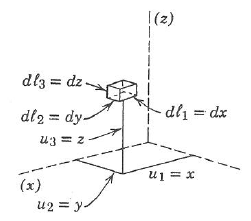
\includegraphics{Waves/waves_f1.png}
\end{figure}

Para las coordenadas cilíndricas tenemos que 

\begin{figure}[H]
    \centering
    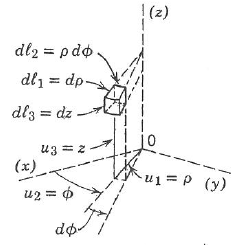
\includegraphics{Waves/waves_f2.png}
\end{figure}

El elemento $dl_2$ corresponde a la longitud de arco de radio $\rho$ y ángulo $d \phi$, de modo que queda

\begin{eqnarray*}
dl_1 = d\rho \\
dl_2 = \rho d\phi \\
dl_3 = dz \\
h_1 = 1 \\
h_2 = \rho \\
h_3 = 1
\end{eqnarray*}

Y para las coordenadas esféricas 
\begin{figure}[H]
    \centering
    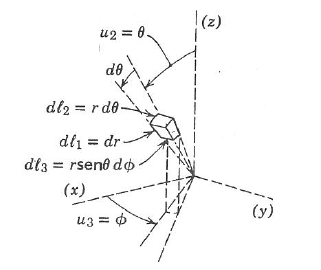
\includegraphics{Waves/waves_f3.png}
\end{figure}

La longitud de arco que corresponde a $dl_3$ corresponde a la proyección del elemento volumétrico sobre el plano $xy$, el radio corresponderá a $r \sin \theta$ y la longitud de arco $r \sin \theta$, por tanto 

\begin{eqnarray*}
dl_1 = d r \\
dl_2 = r d\theta \\
dl_3 = r \sin \theta d \phi \\
h_1 = 1 \\
h_2 = r \\
h_3 = r \sin \theta
\end{eqnarray*}

Finalmente los elementos de volumen quedan

\begin{eqnarray*}
dv = dx \ dy \ dz \\
dv = \rho \ d\rho \ d \phi \ d z \\
dv = r^2 \sin \theta \ dr \ d \theta \ d \phi
\end{eqnarray*}

Un elemento $ds$ de una duperficie en el espacio se puede dejar en su forma escalar $ds$ pero si se desea se puede dar una caracterización vectorial $d \mathbf{s}$. Para el ejemplo de coordenadas esféricas, la forma escalar del elemento de superficie sería

\begin{equation*}
ds = r^2 \sin \theta d \theta \ d \phi
\end{equation*}

la condición vectorial se otorga multiplicando este elemento de superficie con un vector unitario normal al elemento de superficie. 

\begin{equation*}
d \mathbf{s} = \mathbf{a}_{r} ds = \mathbf{a}_{r} r^2 \sin \theta d \theta \ d \phi
\end{equation*}



\subsection{Vector de posición}

Para cada punto en el espacio se puede hacer una notación vectorial, el cual corresponde a un vector desde el origen hasta el punto en cuestión. Para las coordenadas rectangulares,

\begin{equation*}
\mathbf{r} = \mathbf{a}_x x + \mathbf{a}_y y + \mathbf{a}_z z
\end{equation*}

para las coordenadas cilíndricas,

\begin{equation*}
\mathbf{r} = \mathbf{a}_{\rho} \rho + \mathbf{a}_z z
\end{equation*}

y en las coordenadas cilíndricas

\begin{equation*}
\mathbf{r} = \mathbf{a}_r r
\end{equation*}

Una forma de realizar notación de puntos en el espacio es mediante el vector $\mathbf{r}$ es $P(\mathbf{r})$. El elemento diferencial de longitud que separa los puntos $P(\mathbf{r})$ y $P(\mathbf{r} + d \mathbf{r})$ se denota con el elemento diferencial $d \mathbf{r}$ y se define de la siguiente manera:

\begin{equation*}
d \mathbf{r} = \mathbf{a}_1 d l_1 + \mathbf{a}_2 d l_2 + \mathbf{a}_3 d l_3
\end{equation*}

Se forma un paralelepípedo cuyos vértices opuestos está formado por el vector diferencial, y la longitud de este vector está dada por 

\begin{equation*}
d l = \left( (h_1 d u_1)^2 + (h_2 d u_2)^2 + (h_3 d u_3)^2 \right)^{\frac{1}{2}}
\end{equation*}

Como ejemplo, para las coordenadas esféricas, el elemento de línea será

\begin{equation*}
d \mathbf{r} = d \mathbf{l} = \mathbf{a}_r d r + \mathbf{a}_\theta r d \theta + \mathbf{a}_\phi r \sin \theta d \phi  
\end{equation*}

y su longitud es

\begin{equation*}
dl = \sqrt{(dr)^2 + (r d\theta)^2 + (r \sin \theta \ d \phi)^2}
\end{equation*}

\subsection{Integración de vectores}

 Es conveniente examinar con cuidado el integrando de la integral vectorial, porque puede ser un escalar o un vector, por ejemplo la integral de línea 

\begin{equation*}
\int_{l} \mathbf{A} \cdot \mathbf{B} \ d l  
\end{equation*}

 la integral de superficie

\begin{equation*}
\int_S (\mathbf{A} \times \mathbf{B}) \cdot d\mathbf{s}
\end{equation*}

y la integral de volumen

\begin{equation*}
\int_V \mathbf{A} \times \mathbf{B} dv
\end{equation*}

Son elementos escalares, porque tiene integrandos escalares. Por su parte las siguientes integrales

\begin{eqnarray*}
\int_l \mathbf{G} \ d\mathbf{l} \\
\int_S \mathbf{H} \times d \mathbf{s} \\
\int_V \mathbf{J} \times \mathbf{K} \ dv
\end{eqnarray*}

Posee integrandos vectoriales y por tanto sus resultados son vectoriales.

Un ejemplo de gran utilidad es la integral escalar de línea 

\begin{equation*}
\int_l \mathbf{F} \times d \mathbf{l} = \int_l F dl \cos \theta
\end{equation*}

La integral de trabajo. Para las coordenadas generalizadas podemos determinar esta integral de la siguiente manera

\begin{eqnarray*}
\int \mathbf{F} \times d \mathbf{l} &=& \int_l F_1 dl_1 + \int_l F_2 d l_2 + \int_l F_3 d l_3 \\
&=& \int_l F_1 h_1 \ du_1 + \int_l F_2 h_2 \ du_2 + \int_l F_3 h_3 \ du_3
\end{eqnarray*}

\subsection{Cargas eléctricas, corrientes y sus densidades}

Desde el punto de vista del electromagnetismo clásico, se considera a un conjunto de cargas eléctricas como si fuera capaz de dividirse indefinidamente, de manera que la densidad volumétrica de carga, indicada por el símbolo $\rho_v$ y se define:

\begin{equation*}
\rho_v = \frac{\Delta q}{\Delta v} \text{C}/\text{m}^3
\end{equation*}

Dado que la carga que reside dentro de un volumen puede variar de un punto a otro de la región, y también puede variar con el tiempo, la densidad de carga es un campo escalar y se puede escribir como $\rho_v(u_1,u_2,u_3,t)$ o $\rho_v(\mathbf{r},t)$.

También se puede describir la densidad de carga en superficies o en caminos concretos como densidad superficial de carga y densidad lineal de carga $\rho_s$ y $\rho_l$. Las cargas pueden ser  positivas o negativas, y la carga neta siempre será la suma de las cargas positivas y las negativas. 

La cantidad total de carga contenida en una región de volumen, superficie o línea se puede determinar como la integral del campo densidad a lo largo de la región.

\begin{equation*}
q = \int_v \rho_v \ dv
\end{equation*}

Teniendo un campo vectorial en el espacio, podemos definir cualquier superficie y medir la cantidad de líneas del campo que atraviesa dicha superficie. Las líneas de flujo neto $\psi$ que pasan a través de $S$ pueden ser una medida de alguna cantidad física. La cantidad diferencial de flujo $d \psi$ que pasa a través de cualquier elemento superficial $ds$ en el espacio, se define como el producto punto $\mathbf{F} \cdot d \mathbf{s}$. Como consecuencia el flujo neto del campo $\mathbf{F}$ a través de la superficie $S$ es la suma de todos los flujos diferenciales

\begin{equation*}
\psi = \int_S \mathbf{F} \cdot d \mathbf{s}
\end{equation*}

Si la superficie es cerrada, entonces el flujo neto que la atraviesa es

\begin{equation*}
\psi = \oint_S \mathbf{F} \cdot d \mathbf{s}
\end{equation*}


Si se representa una densidad volumétrica de carga $\rho_v$ que está en movimiento con una velocidad promedio $\mathbf{v}$, se puede definir una función de densidad de corriente $\mathbf{J}$ como

\begin{equation*}
\mathbf{J} = \rho_v \mathbf{v} \text{A}/\text{m}^2
\end{equation*}

El flujo de corriente diferencial $di$ que fluye a través de un elemento de superficie $d \mathbf{s}$ en que existe una densidad de corriente $\mathbf{J}$ es $di = \mathbf{J} \cdot d\mathbf{s}$ y la corriente neta es la integral

\begin{equation*}
i = \int_S \mathbf{J} \cdot d \mathbf{s} \ \text{A} 
\end{equation*}

\subsection{Campos eléctricos y magnéticos en función de sus fuerzas}

Los campos electromagnéticos son campos de fuerzas que se originan a partir de cargas eléctricas. Las cargas eléctricas en reposo con respecto a un punto de observación, dan lugar a un campo electrostático. El movimiento relativo de las cargas proporciona un campo de fuerzas adicional llamado magnético, campo magnetostático si las cargas se mueven a una velocidad constante con relación al punto de observación. Y los campos electromagnéticos son los originados por movimientos acelerados de las cargas produciendo campos variables en el tiempo. \\

El símbolo de la intensidad de campo eléctrico o simplemente intensidad eléctrica es $\mathbf{E}$; sus unidades están dadas por fuerza por unidad de carga (Newtons por Coulomb); el campo magnético está representado mediante el vector $\mathbf{B}$ y se denomina densidad de flujo magnético; con unidades de weber por metro cuadrado. Si los campos $\mathbf{E}$ y $\mathbf{B}$ existen en un punto $P$ del espacio, se puede detectar físicamente su presencia mediante una carga $q$ colocada en el punto. La fuerza $\mathbf{F}$ que actúa en esa carga está dada por la \textit{ley de las fuerzas de Lorentz}

\begin{eqnarray*}
\mathbf{F} &=& q(\mathbf{E} + \mathbf{v} \times \mathbf{B}) \\
&=& \mathbf{F}_E + \mathbf{F}_B
\end{eqnarray*}

\subsection{Ecuaciones de Maxwell integrales para campos en el espacio vacío}

Las siguientes son las formas integales de las relaciones entre campos eléctricos y magnéticos y sus distribuciones asociadas de carga y corriente en el espacio vacío

\begin{eqnarray*}
\oint_S (\epsilon_0 \mathbf{E}) \cdot d \mathbf{s} &=& \int_V \rho_v \ dv \\
\oint_S \mathbf{B} \cdot d \mathbf{s} &=& 0 \\
\oint_l \mathbf{E} \cdot d \mathbf{l} &=& - \frac{d}{dt} \int_s \mathbf{B} \cdot d \mathbf{s} \\
\oint_l \frac{\mathbf{B}}{\mu_o} \cdot d \mathbf{l} &=& \int_S \mathbf{J} \cdot d \mathbf{s} + \frac{d}{dt} \int_s (\epsilon_0 \mathbf{E}) \cdot d \mathbf{s}
\end{eqnarray*}

Para campos estáticos la ley de Ampere puede ser escrita de la siguiente manera:
\begin{equation*}
\oint_l \frac{\mathbf{B}}{\mu_o} \cdot d \mathbf{l} = \int_S \mathbf{J} \cdot d \mathbf{s} = i
\end{equation*}


\subsection{Ecuaciones de Maxwell en la forma vectorial diferencial}

Pequeño recordatorio de las coordenadas ortogonales generalizadas de los operadores diferenciales gradientem divergencia y rotacional. También de los teoremas de Stokes y de la divergencia a partir de los cuales se obtienen las ecuaciones en su forma diferencial. 

\subsubsection{Diferenciacion de campos vectoriales}

Definición clásica de la derivada de un campo vectorial para $\mathbf{F}(u)$, su derivada es

\begin{equation*}
\frac{d \mathbf{F}}{d u} = \lim_{\Delta u \to 0} \frac{\mathbf{F}(u + \Delta u)- \mathbf{F}(u)}{\Delta u}
\end{equation*}

Para el caso del producto de una función escalar con una función vectorial, se tiene que

\begin{eqnarray*}
\frac{d f \mathbf{F}}{d u} &=& \lim_{\Delta u \to 0}  \frac{(f+\Delta f)(\mathbf{F}+\Delta \mathbf{F})}{\Delta u} \\
&=& f \frac{d \mathbf{F}}{d u} + \mathbf{F} \frac{df}{du}
\end{eqnarray*}

Si la función vectorial es de varias variables, y tiene derivadas parciales continuas de al menos segundo orden, es permisible diferenciarlo en cualquier orden, así

\begin{equation*}
\frac{\partial^{2} \mathbf{F}}{\partial u_1 \partial u_2} = \frac{\partial \mathbf{F}}{\partial u_2 \partial u_1}
\end{equation*}

Las siguientes propiedades son comprobales:

\begin{eqnarray*}
 \frac{\partial (f\mathbf{F})}{\partial t} &=& f \frac{\partial \mathbf{F}}{\partial t} + \mathbf{F} \frac{\partial f}{\partial t} \\
 \frac{\partial (\mathbf{F} \cdot \mathbf{G})}{\partial t} &=& \mathbf{F} \cdot \frac{\partial \mathbf{G} }{\partial t } + \mathbf{G} \cdot \frac{\partial \mathbf{F} }{\partial t } \\
 \frac{\partial (\mathbf{F} \times \mathbf{G})}{\partial t} &=& \mathbf{F} \times \frac{\partial \mathbf{G} }{\partial t } + \frac{\partial \mathbf{F} }{\partial t } \times \mathbf{G}
\end{eqnarray*}

\subsubsection{Gradiente}

Es un operador que sirve para determinar la rapidez de cambio en el espacio de un campo escalar.
para las coordenadas cartesianas, y para las generalizadas como sigue

\begin{equation*}
\textbf{grad} f \equiv \mathbf{a}_1 \frac{1}{h_1} \frac{\partial f }{\partial  u_1} + \mathbf{a}_2 \frac{1}{h_2} \frac{\partial f }{\partial u_2} + \mathbf{a}_3 \frac{1}{h_3} \frac{\partial f }{\partial u_3 }
\end{equation*}

El vector (o función vectorial) gradiente $\textbf{grad} f$ indica tanto la magnitud como la dirección de la máxima rapidez espacial de cambio de $f$ en cualquier punto en una región.

Una propiedad importante: la integral cerrada de línea del gradiente de cualquier función es nula:

\begin{equation*}
\oint_l (\textbf{grad} (f)) \cdot d \mathbf{l} = 0
\end{equation*}

para cualquier función escalar $f$ bien definida.

Otra definición importante del gradiente de una función de varias variables es que si una ecuación $F(x,y,z)=0$ es la ecuación de una superficie y $F$ es diferenciable, y $F_x$, $F_y$ y $F_z$ no son todas cero en el punto $P_0(x_0,y_0,z_0)$, entonces 

\begin{equation*}
\textbf{grad}F(x_0,y_0,z_0)
\end{equation*}

es un vector normal a $S$ en $P_0$


\subsubsection{Operador Nabla}

 Definamos el operador nabla para las coordenadas cartesianas

\begin{equation*}
\nabla \equiv \mathbf{a}_x \frac{\partial  }{\partial  x} + \mathbf{a}_y \frac{\partial  }{\partial y } + \frac{\partial  }{\partial z }\mathbf{a}_z
\end{equation*}

El gradiente de un campo escalar se define mediante el operador nabla como sigue

\begin{equation*}
\textbf{grad}(f) \equiv  \nabla f = \mathbf{a}_x \frac{\partial f }{\partial  x} + \mathbf{a}_y \frac{\partial f }{\partial y } + \frac{\partial f }{\partial z }\mathbf{a}_z
\end{equation*}


Se puede generalizar el operador nabla para las coordenadas ortogonales generalizadas de la siguiente manera

\begin{equation*}
\nabla 
\left\{
\begin{aligned}
V \\
\cdot \mathbf{A} \\
\times \mathbf{A}
\end{aligned}
\right\} = \frac{1}{h_1 h_2 h_3} \left[ 
    \frac{\partial }{\partial u_1} \left( h_2 h_3 \mathbf{a}_1 
    \left\{
    \begin{aligned}
    V \\
    \cdot \mathbf{A} \\
    \times \mathbf{A}
    \end{aligned}
    \right\} \right) 
    + \frac{\partial }{\partial u_2} \left( h_3 h_1 \mathbf{a}_2 
    \left\{
    \begin{aligned}
    V \\
    \cdot \mathbf{A} \\
    \times \mathbf{A}
    \end{aligned}
    \right\} \right) 
    + \frac{\partial }{\partial u_3} \left( h_1 h_2 \mathbf{a}_3 
    \left\{
    \begin{aligned}
    V \\
    \cdot \mathbf{A} \\
    \times \mathbf{A}
    \end{aligned}
    \right\} \right) 
\right]
\end{equation*}


\subsubsection{Otra definición de divergencia}

Sea una función o campo vectorial $\mathbf{F}$. La divergencia puede definirse como el límite dek flujo neto hcia afuera de $\mathbf{F}$, por volumen unitario, conforme el volumen $\Delta v$ encerrado por la superficie $S$ tiende a cero:

\begin{equation*}
\text{div} \mathbf{F} \equiv \lim_{\Delta v \to 0} \frac{\oint_S \mathbf{F} \cdot d \mathbf{s}}{\Delta v}
\end{equation*}

De forma diferencial la definición de divergencia para las coordenadas ortogonales generalizadas:

\begin{equation*}
\text{div} \mathbf{F} = \frac{1}{h_1 h_2 h_3} \left[ \frac{\partial (F_1h_2h_3) }{\partial u_1 } + \frac{\partial (F_2h_1h_3) }{\partial u_2 } + \frac{\partial (F_3h_1h_2) }{\partial u_3 } \right]
\end{equation*}

A partir de la definición de divergencia anteriormente dada, volvemos a la ley de Gauss para campos eléctricos

\begin{equation*}
\oiint_S \left( \epsilon_0 \mathbf{E} \right) \cdot d \mathbf{s} = \iiint_V \rho_v \ dv
\end{equation*}

Tomando esta ecuación y dividiendo entre elementos volumétricos $\Delta v$,

\begin{equation*}
\frac{\oiint_S \left( \epsilon_0 \mathbf{E} \right) \cdot d \mathbf{s}}{\Delta v} = \frac{\iiint_V \rho_v \ dv}{\Delta v}
\end{equation*}

Se tiene del lado izquierdo de la ecuación la definición de la divergencia; y del lado derecho, la densidad volumétrica, en el límite de $\Delta v \to 0$:

\begin{equation*}
\nabla \cdot ( \epsilon_0 \mathbf{E} ) = \rho_v 
\end{equation*}

Y para la ley de Gauss para el campo magnético

\begin{equation*}
\oiint_S \mathbf{B} \cdot d \mathbf{s} = 0
\end{equation*}

Realizaando el procedimiento similar, se tiene

\begin{equation*}
\nabla \cdot \mathbf{B} = 0
\end{equation*}


\subsubsection{Definición generalizada para el rotacional}

Dentro de las coordenadas ortogonales generalizadas, el rotacional de un campo $\mathbf{F}$ denotado por 

\begin{equation*}
\text{rot} \mathbf{F} = \nabla \times \mathbf{f}
\end{equation*}

Se puede calcular mediante el determinante de la matriz

\begin{equation*}
\text{rot } \mathbf{F} = 
\left|
\begin{matrix}
    \frac{ \mathbf{a}_1 }{h_2  h_3  } & \frac{ \mathbf{a}_2 }{h_3  h_1  } & \frac{ \mathbf{a}_3 }{h_1  h_2  } \\
    \frac{\partial }{\partial u_1} & \frac{\partial }{\partial u_2} & \frac{\partial }{\partial u_3} \\
    h_1 F_1 & h_2 F_2 & h_3 F_3 
\end{matrix}
\right| \equiv \nabla \times \mathbf{F}
\end{equation*}

\subsubsection{Relaciones del rotacional de Maxwell para campos eléctricos y magnéticos en el espacio vacíos}

Tomando como base la ecuación de la ley de Ampere y la definición de rotacional, se llega a que, para cada componente coordenado $a_i$

\begin{equation*}
\mathbf{a_i} \frac{\oint_l \mathbf{E} \cdot d \mathbf{l} }{\Delta s_1} = \mathbf{a_i} \frac{-\frac{d}{dt}\int_{\Delta s_1} \mathbf{B} \cdot d \mathbf{s}}{\Delta s_1}
\end{equation*}

Donde la combinación vectorial de cada componente coordenado da como resultado la rotacional total, se llega a que

\begin{equation*}
\nabla \times \mathbf{E} = - \frac{\partial \mathbf{B}}{\partial t}
\end{equation*}

El cual es la forma diferencial de la ley de Ampere. Y de manera análoga

\begin{equation*}
\nabla \times \frac{\mathbf{B}}{\mu_0} = \mathbf{J} + \frac{\partial (\epsilon_0 \mathbf{E}) }{\partial t}
\end{equation*}

























\subsection{Ecuaciones de Maxwell con forma compleja armónica en el tiempo}

Las formas integrales de las ecuaciones de Maxwell son adecuadas para encontrar las soluciones de distribuciones de cargas estáticas o corrientes que tengan simetrías somples, aunque desafortunadamente los métodos que se apoyan en la simetría están limitados a unos pocos problemas aislados. Generalmente las formas diferenciales de las ecuaciones de Maxwell ofrecen una clase mucho más amplia de soluciones.

Las soluciones sinusoidales de estado estable o armónicas en el tiempo de las ecuaiones de Maxwell también son de importancia. Los campos $\mathbf{E}$ y $\mathbf{B}$ armónicos en el tiempo, se generan siempre que skus fuentes de carga tengan densidades qkue varían de form sinusoidal en el tiempo. Supongamos que las ondas sinusoidales están en estado estable, entonces $\mathbf{B}$ y $\mathbf{E}$ varían con el factor $\cos (\omega t  + \theta_e)$ y $\cos (\omega t  + \theta_b)$. Una formulación equivalente se logra si el factor se escribe de la forma $e^{i \omega t}$. De modo que se pueden escribir los campos de la siguient forma

\begin{eqnarray*}
\mathbf{E} \equiv \mathbf{\hat{E}} (u_1,u_2,u_3) e^{i \omega t} \\
\mathbf{B} \equiv \mathbf{\hat{B}} (u_1,u_2,u_3) e^{i \omega t} \\
\mathbf{J} \equiv \mathbf{\hat{J}} (u_1,u_2,u_3) e^{i \omega t} \\
\rho_v \equiv \rho_v (u_1,u_2,u_3) e^{i \omega t} 
\end{eqnarray*}

Escribiendo las ecuaciones de maxwell con esta forma de los campos tenemos

\begin{eqnarray*}
\nabla \cdot (\epsilon_0 \mathbf{\hat{E}}) = \hat{\rho_v} \\
\nabla \cdot \mathbf{\hat{B}} = 0  \\
\nabla \times \mathbf{\hat{E}} = - i \omega \mathbf{\hat{B}} \\
\nabla \times \frac{\mathbf{\hat{B}}}{\mu_0} = \mathbf{\hat{J}} + i \omega \epsilon_0 \mathbf{\hat{E}}
\end{eqnarray*}

Las cuales son las ecuaciones deseadas de maxwell complejas armónicas en el tiempo para el espacio vacío. Al encontrar las soluciones complejas de los cambios podemos establecer que la parte real de dicha solución comprende la solución sinusoidal:

\begin{eqnarray*}
\mathbf{E} (u_1,u_2,u_3,t) = \text{Re} \{ \mathbf{\hat{E}}(u_1,u_2,u_3) e^{i \omega t} \} \\
\mathbf{B} (u_1,u_2,u_3,t) = \text{Re} \{ \mathbf{\hat{B}}(u_1,u_2,u_3) e^{i \omega t} \}
\end{eqnarray*}

\subsection{Operador laplaciano y rot rot}

El operador laplaciano surge de calcular la divergencia de un gradiente, el gradiente de $f$ es 

\begin{equation*}
\nabla f = \mathbf{a}_1 \frac{1}{h_1} \frac{\partial f}{\partial u_1} + \mathbf{a}_2 \frac{1}{h_2} \frac{\partial f}{\partial u_2} + \mathbf{a}_3 \frac{1}{h_3} \frac{\partial f}{\partial u_3}
\end{equation*}

su divergencia es

\begin{equation*}
\nabla \cdot (\nabla f) \equiv \nabla^2 f= \frac{1}{h_1 h_2 h_3} \left[ \frac{\partial}{\partial u_1} \left( \frac{h_2 h_3 }{h_1 } \frac{\partial f}{\partial u_1} \right) + \frac{\partial}{\partial u_2} \left( \frac{h_1 h_3 }{h_2 } \frac{\partial f}{\partial u_2} \right) + \frac{\partial}{\partial u_3} \left( \frac{h_1 h_2 }{h_3 } \frac{\partial f}{\partial u_3} \right) \right] 
\end{equation*}

Para las coordenadas rectangulares esto puede escribirse como

\begin{equation*}
\nabla \cdot (\nabla f) = \nabla^2 f = \frac{\partial^2 f }{\partial x^2} + \frac{\partial^2 f }{\partial y^2} + \frac{\partial^2 f}{\partial z^2}
\end{equation*}

Por otro lado, considerando el gradiente de la divergencia, $\nabla (\nabla \cdot \mathbf{F})$ tenemos lo siguiente

\begin{equation*}
\nabla^2 \mathbf{F} \equiv \frac{1}{h_1 h_2 h_3} \left[ \frac{\partial}{\partial u_1} \left( \frac{h_2 h_3 }{h_1 } \frac{\partial }{\partial u_1} \right) + \frac{\partial}{\partial u_2} \left( \frac{h_1 h_3 }{h_2 } \frac{\partial }{\partial u_2} \right) + \frac{\partial}{\partial u_3} \left( \frac{h_1 h_2 }{h_3 } \frac{\partial }{\partial u_3} \right) \right] \mathbf{\times} (\mathbf{a}_1 F_1 + \mathbf{a}_2 F_2 + \mathbf{a}_3 F_3) 
\end{equation*}

Para las coordenadas rectangulares tenemos

\begin{equation*}
\nabla^2 \mathbf{F} = \mathbf{a}_x \nabla^2 F_x + \mathbf{a}_y \nabla^2 F_y + \mathbf{a}_z \nabla^2 F_z 
\end{equation*}

Como ejemplo, para el sistema cilíndtrico se tiene que su laplaciano vectorial es

\begin{equation*}
\nabla^2 \mathbf{F} = \mathbf{a}_\rho \left( \nabla^2 F_\rho - \frac{2}{\rho^2} \frac{\partial F_\phi}{\partial \phi} - \frac{F_\rho}{\rho^2} \right) + \mathbf{a}_\phi \left( \nabla^2 F_\phi  - \frac{2}{\rho^2} \frac{\partial F_\rho}{\partial \phi} - \frac{F_\phi}{\rho^2} \right)+ \mathbf{a}_z \nabla^2 F_z 
\end{equation*}

También existe para campos, calcular el rotacional del rotacional, que sería $\nabla  \times (\nabla \times \mathbf{F})$, debido a su complejidad, miremos solo el resultado re calcular este operador en coordenadas rectangulares:

\begin{eqnarray*}
\nabla \times (\nabla \times \mathbf{F}) = \mathbf{a}_x \left( \frac{\partial  }{\partial y } \left( \frac{\partial F_y }{\partial x } - \frac{\partial F_x }{\partial y } \right) - \frac{\partial  }{\partial z } \left( \frac{\partial F_x }{\partial z} - \frac{\partial F_z }{\partial x } \right) \right) + \mathbf{a}_y \left( \frac{\partial  }{\partial z } \left( \frac{\partial F_z }{\partial y } - \frac{\partial F_y }{\partial z } \right) - \frac{\partial  }{\partial x } \left( \frac{\partial F_y }{\partial x } - \frac{\partial F_x }{\partial y } \right) \right) \\
+ \mathbf{a}_z \left( \frac{\partial  }{\partial x } \left( \frac{\partial F_x }{\partial z } - \frac{\partial F_z }{\partial x } \right) - \frac{\partial  }{\partial y } \left( \frac{\partial F_z }{\partial y } - \frac{\partial F_y }{\partial z } \right) \right)
\end{eqnarray*}

Comparando los términos de esta expresión con la rotacional de la rotacional, y haciendo sumas de manera apropiada, se llega a la conclusión de que 

\begin{equation*}
\nabla \times (\nabla \times \mathbf{F}) = \nabla (\nabla \cdot \mathbf{F}) - \nabla^2 \mathbf{F}
\end{equation*}

Especialmente si el campo vectorial $\mathbf{F}$ no es divergente ($\nabla \cdot \mathbf{F} = 0$), se tiene una expresión útil para el rotacional del rotacional:

\begin{equation*}
\nabla \times (\nabla \times \mathbf{F}) = - \nabla^2 \mathbf{F}
\end{equation*}

La siguiente tabla proporciona un resumen útila de algunas identidadea vectoriales algebráicas, integrales y diferenciales:

\begin{figure}[H]
    \centering
    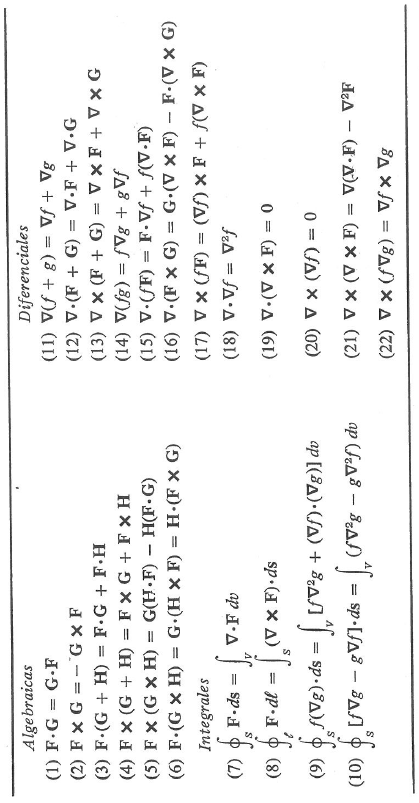
\includegraphics[scale=0.7, angle=-90]{Waves/waves_f4.png}
\end{figure}

\subsection{Teoremas integrales de Green}

Recordemos el teorema de la divergencia

\begin{equation*}
\oiint_s \mathbf{F} \cdot d \mathbf{S} = \iiint_v (\nabla \cdot \mathbf{F}) \ d V
\end{equation*}

si se especializa este teorema a una clase determinada de funciones vectoriales y obtener las identidades conocidas como los teoremas de Green.

Sea $\mathbf{F}$ un campo vectorial tal que $\mathbf{F}= f \mathbf{\nabla}g$, es decir, $\mathbf{F}$ es campo conservativo.

Aplicamos el teorema de divergencia a este campo

\begin{equation*}
\oiint_s (f \mathbf{\nabla}g) \cdot d \mathbf{S} = \iiint_v (\nabla \cdot (f \mathbf{\nabla}g)) \ d V
\end{equation*}

usamos las propiedades vectoriales y queda

\begin{equation*}
\oiint_s (f \mathbf{\nabla}g) \cdot d \mathbf{S} =  \iiint_v \left( f \nabla^2 g + (\nabla f) \cdot (\nabla g) \right) \ d V
\end{equation*}

Es la primera identidad integral de Green.

Por su parte, sea $\mathbf{G}= g \nabla f$, aplicando teorema de divergencia, obtenemos

\begin{equation*}
\oiint_s (g \mathbf{\nabla}f) \cdot d \mathbf{S} =  \iiint_v \left( g \nabla^2 f + (\nabla g) \cdot (\nabla f) \right) \ d V
\end{equation*}

Restamos las anteriores

\begin{eqnarray*}
\oiint_s (f \mathbf{\nabla}g) \cdot d \mathbf{S} - \oiint_s (g \mathbf{\nabla}f) \cdot d \mathbf{S} &=& \iiint_v \left( f \nabla^2 g + (\nabla f) \cdot (\nabla g) \right) \ d V - \iiint_v \left( g \nabla^2 f + (\nabla g) \cdot (\nabla f) \right) \ d V \\
\oiint_s (f \mathbf{\nabla}g - g \mathbf{\nabla}f ) \cdot d \mathbf{S} &=& \iiint_v \left( f \nabla^2 g + (\nabla f) \cdot (\nabla g) - \left( g \nabla^2 f + (\nabla g) \cdot (\nabla f) \right) \right) dV \\
\oiint_s (f \mathbf{\nabla}g - g \mathbf{\nabla}f ) \cdot d \mathbf{S} &=& \iiint_v \left( f \nabla^2 g - g \nabla^2 f \right) dV \\
\end{eqnarray*}

Esta es el teorema simétrico de Green.

Este teorema sirve para probar y demostrar que si dos funciones tienen el mismo rotacional y divergencia, entonces estas dos funciones son iguales y por lo tanto es una funcipon única.

\subsection{Ecuaciones de onda para campos eléctricos y magnéticos}

Volvamos a escribir las ecuaciones de Maxwell:

\begin{eqnarray*}
\nabla \cdot (\epsilon_0 \mathbf{E}) &=& \rho_v \\
\nabla \cdot \mathbf{B} &=& 0 \\
\nabla \times \mathbf{E} &=& - \frac{\partial \mathbf{B}}{\partial t} \\
\nabla \times \frac{\mathbf{B}}{\mu_0} &=& \mathbf{J} + \epsilon_0 \frac{\partial \mathbf{E}}{\partial t} 
\end{eqnarray*}

Tomemos rotacional a ambos lados de 

\begin{eqnarray*}
\nabla \times \mathbf{E} &=& - \frac{\partial \mathbf{B}}{\partial t} \\
\nabla \times \left( \nabla \times \mathbf{E} \right) &=& \nabla \times \left( - \frac{\partial \mathbf{B}}{\partial t} \right) \\
\nabla \times \left( \nabla \times \mathbf{E} \right) &=& - \frac{\partial \left( \nabla \times \mathbf{B} \right)}{\partial t} \\
\nabla \times \left( \nabla \times \mathbf{E} \right) &=& - \frac{\partial}{\partial t} \left( \nabla \times \mathbf{B} \right)
\end{eqnarray*}

De la otra ecuación de Maxwell:

\begin{eqnarray*}
\nabla \times \frac{\mathbf{B}}{\mu_0} &=& \mathbf{J} + \epsilon_0 \frac{\partial \mathbf{E}}{\partial t} \\
\nabla \times \mathbf{B} &=& \mu_0 \mathbf{J} +  \mu_0 \epsilon_0 \frac{\partial \mathbf{E}}{\partial t} 
\end{eqnarray*}

y reemplazamos $\nabla \times \mathbf{B}$:

\begin{eqnarray*}
\nabla \times \left( \nabla \times \mathbf{E} \right) &=& - \frac{\partial}{\partial t} \left( \mu_0 \mathbf{J} +  \mu_0 \epsilon_0 \frac{\partial \mathbf{E}}{\partial t}  \right) \\
\nabla \times \left( \nabla \times \mathbf{E} \right) + \mu_0 \epsilon_0 \frac{\partial^2 \mathbf{E}}{\partial t^2} &=& -\mu_0 \frac{\partial \mathbf{J}}{\partial t}
\end{eqnarray*}

Vemos que esta es una ecuación diferencial parcial vectorial que se conoce como ecuación no homogénea vectorial de onda para el espacio vacío. 

Realizando un procedimiento y susticuciones similares para las otras ecuaciones de Maxwell llegamos a una segunda ecuación de 

\begin{equation*}
\nabla \times \left( \nabla \times \mathbf{B} \right) + \mu_0 \epsilon_0 \frac{\partial^2 \mathbf{B}}{\partial t^2} = \mu_0 \nabla \times \mathbf{J}
\end{equation*}

Si el campo eléctrico no es divergente ($\nabla \cdot \mathbf{E}=0$), entonces el término $\nabla \times (\nabla \times \mathbf{E})$ se reduce a $-\nabla^2 \mathbf{E}$; más aún, si el campo no es divergente en la región, significa que la región está libre de cargas ($\rho_v=0$). Adicionalmente sabemos que el campo magnético es siempre divergente, entonces podemos escribir las ecuaciones de onda de la siguiente forma

\begin{eqnarray*}
\nabla^2 \mathbf{E} - \mu_0 \epsilon_0 \frac{\partial^2 \mathbf{E}}{\partial t^2} &=& \mu_0 \frac{\partial \mathbf{J}}{\partial t} \\
\nabla^2 \mathbf{B} - \mu_0 \epsilon_0 \frac{\partial^2 \mathbf{B}}{\partial t^2} &=& -\mu_0 \nabla \times \mathbf{F}
\end{eqnarray*}


Si la región es el espacio vacío, es decir, $\mathbf{J}=0$, se pueden obtener las siguientes ecuaciones 

\begin{eqnarray*}
\nabla^2 \mathbf{E} - \mu_0 \epsilon_0 \frac{\partial^2 \mathbf{E}}{\partial t^2} &=& 0 \\
\nabla^2 \mathbf{B} - \mu_0 \epsilon_0 \frac{\partial^2 \mathbf{B}}{\partial t^2} &=& 0
\end{eqnarray*}

las cuales son las ecuaciones homogéneas vectoriales de onda para el espacio vacío.\\


Miremos el caso para coordenadas cartesianas:

\begin{eqnarray*}
\nabla^2 E_x - \mu_0 \epsilon_0 \frac{\partial^2 E_x}{\partial t^2} &=& 0 \\
\nabla^2 E_y - \mu_0 \epsilon_0 \frac{\partial^2 E_y}{\partial t^2} &=& 0 \\
\nabla^2 E_z - \mu_0 \epsilon_0 \frac{\partial^2 E_z}{\partial t^2} &=& 0 
\end{eqnarray*}

\begin{eqnarray*}
\nabla^2 B_x - \mu_0 \epsilon_0 \frac{\partial^2 B_x}{\partial t^2} &=& 0 \\
\nabla^2 B_y - \mu_0 \epsilon_0 \frac{\partial^2 B_y}{\partial t^2} &=& 0 \\
\nabla^2 B_z - \mu_0 \epsilon_0 \frac{\partial^2 B_z}{\partial t^2} &=& 0 
\end{eqnarray*}

Si tenemos los campos $\mathbf{E}=e^{i \omega t}\mathbf{\hat{E}}$, entonces obtenemos

\begin{eqnarray*}
\nabla^2 \hat{E}_x + \omega^2 \mu_0 \epsilon_0 \hat{E}_x &=& 0 \\
\nabla^2 \hat{E}_y + \omega^2 \mu_0 \epsilon_0 \hat{E}_y &=& 0 \\
\nabla^2 \hat{E}_z + \omega^2 \mu_0 \epsilon_0 \hat{E}_z &=& 0
\end{eqnarray*}

\begin{eqnarray*}
\nabla^2 \hat{B}_x + \omega^2 \mu_0 \epsilon_0 \hat{B}_x &=& 0 \\
\nabla^2 \hat{B}_y + \omega^2 \mu_0 \epsilon_0 \hat{B}_y &=& 0 \\
\nabla^2 \hat{B}_z + \omega^2 \mu_0 \epsilon_0 \hat{B}_z &=& 0
\end{eqnarray*}

Las soluciones más simples de esas ecuaciones escalares de onda son ondas planas uniformes que comprenden hasta solo dos componentes.

\subsection{Ondas planas uniformes en es espacio vacío} \label{Ondas_planas_uniformes_en_es_espacio_vacio}

Las propiedades de simplificación son que las soluciones se prestan al sistema de coordenadas rectangulares y que el número de componentes de canpo se reduce a un mínimo de dos. con estas propiedades, las soluciones de onda mas simples son ondas planas uniformes.

las ondas tienen la propiedad de que en cualquier instante fijo los campos eléctricos y magnéticos son uniformes sobre superficies planas. Los planos son escogidos arbitrariamente. de manera que están definidos para $z=C$ constante lo que equivale a expresar que las variaciones espaciales de los campos eléctrico y magnético son cero sobre los planos $z=C$ esto conlleva a lo siguiente:

\begin{enumerate}
    \item Los campos no dependen de $x$ ni de $y$, es es que $\frac{\partial }{\partial x} = \frac{\partial }{\partial y} = 0$ para todas las componentes del campo.
    \item En toda la región las densidades de carga y de corriente son cero.
\end{enumerate}

Con estas suposiciones, las ecuaciones de maxwell quedan de la siguiente forma

\begin{eqnarray*}
\nabla \cdot (\epsilon_0 \mathbf{\hat{E}} ) = 0 \\
\nabla \cdot \mathbf{\hat{B}} = 0 \\
\nabla \times \hat{E} = - i \omega \mathbf{\hat{B}} \\
\nabla \times \frac{\mathbf{\hat{B}}}{\mu_0} = i \omega \epsilon_0 \mathbf{\hat{E}}
\end{eqnarray*}

Sabemos que combinando las ecuaciones anteriores llegamos a 

\begin{eqnarray*}
\nabla^2 \mathbf{\hat{E}} + \omega^2 \mu_0\epsilon_0 \mathbf{\hat{E}} = 0\\
\nabla^2 \mathbf{\hat{B}} + \omega^2 \mu_0\epsilon_0 \mathbf{\hat{B}} = 0
\end{eqnarray*}


Teniendo en cuenta las suposiciones anteriores de que  $\frac{\partial }{\partial x} = \frac{\partial }{\partial y} = 0$ , podemos ver para las rotacionales lo siguiente

\begin{equation*}
\nabla \times \mathbf{\hat{E}} = - i \omega (\mathbf{a}_x \hat{B}_x + \mathbf{a}_y \hat{B}_y  + \mathbf{a}_z \hat{B}_z )
\end{equation*}

conlleva a 

\begin{eqnarray*}
-\frac{\partial \hat{E}_y}{\partial z} = - i \omega \hat{B}_x \\
\frac{\partial \hat{E}_x}{\partial z} = - i \omega \hat{B}_y \\
\hat{B}_z = 0
\end{eqnarray*}

y de forma similar 


\begin{eqnarray*}
-\frac{\partial \hat{B}_y}{\partial z} = i \omega \mu_0\epsilon_0 \hat{E}_x \\
\frac{\partial \hat{B}_x}{\partial z} = i \omega \mu_0\epsilon_0 \hat{E}_y \\
\hat{E}_z = 0
\end{eqnarray*}

Como se puede ver, no existe componente en $z$ de ningún campo, y que se obtienen dos pares independientes de campos soluciones. 

Por ejemplo, si hacemos $\hat{E}_y = 0$, obtenemos que se eliminan dos de las cuatro ecuaciones, y se obtiene el siguiente sistema

\begin{eqnarray*}
\frac{\partial \hat{E}_x}{\partial z} = - i \omega \hat{B}_y \\
-\frac{\partial \hat{B}_y}{\partial z} = i \omega \mu_0\epsilon_0 \hat{E}_x 
\end{eqnarray*}


Combinando estas ecuaciones para obtener una ecuación que solo dependa de uno de los componentes, obtenemos la siguiente ecuación diferencial


\begin{equation*}
\frac{\partial^2 \hat{E}_x}{\partial z^2} + \omega^2 \mu_0\epsilon_0 \hat{E}_x = 0
\end{equation*}

Esta ecuación es de una sola variable y su solución está dada por

\begin{eqnarray*}
\hat{E_x}(z) = \hat{C_1} e^{-i \beta_0 z} + \hat{C_2} e^{i \beta_0 z}
\end{eqnarray*}

donde el término $\beta_0$ se denomina \textit{constante de fase}

\begin{equation*}
\beta_0 = \omega \sqrt{\mu_0 \ \epsilon_0 }
\end{equation*}

estas soluciones exponenciales complejas son representaciones de ondas de amplitud constante que viajan en las direcciones positiva y negativa de z. Los coeficientes complejos $ \hat{C_1}$ y $ \hat{C_2}$ deben tener las unidades de voltios por metro para denotar amplitudes complejas de las ondas que viajan en sentido positivo y negativo del eje $z$. por tanto empleamos una notación más adecuada

\begin{equation*}
\hat{E_x} (z) = \hat{E}_m^+ e^{-i \beta_0 z} + \hat{E}_m^- e^{i \beta_0 z}
\end{equation*}

Ahora reemplazando esta solución para determinar el campo magnético

\begin{eqnarray*}
\hat{B}_y &=& -\frac{1}{i \omega} \frac{\partial \hat{E}_x}{\partial z} \\
\hat{B}_y &=& -\frac{1}{i \omega} (- i \beta_0 \hat{E}_m^+ e^{-i \beta_0 z} + i \beta_0 \hat{E}_m^- e^{i \beta_0 z}) \\
\hat{B}_y &=& \frac{\beta_0}{\omega} \hat{E}_m^+ e^{-i \beta_0 z} - \frac{\beta_0}{\omega} \hat{E}_m^- e^{i \beta_0 z} \\
\hat{B}_y &=& \sqrt{\mu_0\epsilon_0} \hat{E}_m^+ e^{-i \beta_0 z} - \sqrt{\mu_0\epsilon_0} \hat{E}_m^- e^{i \beta_0 z}
\end{eqnarray*}

La parte real de la solución del campo eléctrico se puede expresar como

\begin{eqnarray*}
E_x(z,t) &=& \text{Re} \{ \hat{E}_x(x) e^{i \omega t} \}  \\
E_x(z,t) &=& E_m^+ \cos (\omega t - \beta_0 z + \phi^+) + E_m^- \cos (\omega t + \beta_0 z + \phi^-)
\end{eqnarray*}

Esto teniendo en cuenta que las constantes $\hat{E}_m^+$ y $\hat{E}_m^-$ sean números complejos cuyas fases (ángulos) son $\phi^+$ y $\phi^-$ respectivamente.

\begin{eqnarray*}
\hat{E}_m^+ = E_m^+ e ^(i \phi^+) \\
\hat{E}_m^- = E_m^- e ^(i \phi^-) 
\end{eqnarray*}


De manera similar tenemos la solución para el campo magnético 


\begin{eqnarray*}
B_x(z,t) &=& \sqrt{\mu_0\epsilon_0} E_m^+ \cos (\omega t - \beta_0 z + \phi^+) + \sqrt{\mu_0\epsilon_0} E_m^- \cos (\omega t + \beta_0 z + \phi^-)
\end{eqnarray*}

el factor de fase determina la longitud de onda, que significa la distancia que debe recorrer la onda para alzancar $2 \pi$ radianes.

\begin{equation*}
\beta_0 \lambda = 2 \pi
\end{equation*}


Por tanto, la longitud de onda es


\begin{equation*}
\lambda = \frac{2 \pi}{\beta_0} = \frac{2 \pi}{\omega \sqrt{\mu_0\epsilon_0}} = \frac{c}{m}
\end{equation*}


la velocidad de fase está dada por 


\begin{eqnarray*}
v_p &=& \frac{\omega}{\beta_0} \\
v_p &=& \frac{1}{\sqrt{\mu_0\epsilon_0}}
\end{eqnarray*}

Esta velocidad es la velocidad de la luz en el espacio vacío, $c$.


Si se define el campo de intensidad magnética $\mathbf{H} = \frac{\mathbf{B}}{\mu_0}$, se tiene que 

\begin{eqnarray*}
\frac{\hat{E}_x^+ (z)}{\hat{H}_y^+ (z)} = \mu_0 \ c = \sqrt{\frac{\mu_0}{\epsilon_0}} \equiv \eta_0 \approx 120 \pi \Omega \\
 = - \frac{\hat{E}_x^- (z)}{\hat{H}_y^- (z)}
\end{eqnarray*}

$\eta_0$ se define como la impedancia intrínseca de onda para el espacio vacío 


\section{Campos electromagnéticos para regiones materiales en estado de reposo}

\subsection{Conductividad eléctrica de los materiales}

El comportamiento de los campos se caracteriza por considerar tres efectos

\begin{enumerate}
    \item Conducción de carga eléctrica.
    \item Polarización eléctrica.
    \item Polarización magnética.
\end{enumerate}

esos efectos se describen de forma adecuada mediante tres parámetros: la conductividad eléctrica $\sigma$, la permitividad eléctrica $\epsilon$ y la permeabilidad magnética $\mu$.

los materiales pueden ser clasificados en función de sus propiedades de conducción eléctrica con aislantes, que esencialmente no posee ningún electrón libre para dar corriente bajo un campo eléctrico, y conductores; los cuales sí poseen una gran cantidad de electrones libres de órbitas externas para producir una corriente de conducción bajo un campo eléctrico. 

A escalas moleculares y atómicas, un sólido eléctricamente conductor se visualiza como una red de iones positivos en los que los electrones de la órbitas externas pueden moverse aleatoriamente. Sobre esta estructura están superpuestas agitaciones térmicas asociadas con la temperatura del conductor. Estos electrones libres se mueven con velocidades distribuidas aleatoriamente, con una velocidad media de

\begin{equation*}
v_d = \frac{1}{N} \sum_{i=1}^{N} v_i
\end{equation*}


promediada en cualquier instante sobre un número grande de partículas en el elemento de volumen. Esta velocidad promedio se denomina velocidad de deriva y es cero en ausencia de un campo eléctrico.

El tiempo llamado tiempo libre medio $\tau_c$, es el intervalo promedio entre las colisiones en un elemento de volumen. Cuando los electrones chocan con la red de iones, ceden en promedio un impulso $m v_d$ en el tiempo libre medio, y la razón promediada de transferencia de impulso a la red de iones por electrón es $\frac{m v_d}{\tau_c}$ N de fuerza, si se iguala esta con la fuerza debida a la ley de Lorentz, se tiene

\begin{equation*}
\frac{m \mathbf{v}_d}{\tau_c} = -e \mathbf{E}
\end{equation*}

 lo cual deja

 \begin{equation*}
\mathbf{v}_d = - \frac{e \tau_c}{m} \mathbf{E}
 \end{equation*}

 esta ecuación relaciona directamente la velocidad de deriva con el campo aplicado. Vemos que es proporcional al campo y que 

 \begin{equation*}
\mu_e = \frac{e \tau_e}{m} \frac{\text{m}^2}{\text{V-s}}
 \end{equation*}

 Rcordemos que la densidad de corriente está dada por 

 \begin{equation*}
\mathbf{J} = \rho_v \mathbf{v}_d
 \end{equation*}

 teniendo que $\rho_v = n e$, donde $n$ es la densidad de electrones libres por metro cúbico (número de $e^-$ por unidad de volumen), la anterior ecuación se escribe como sigue

 \begin{equation*}
\mathbf{J} = \rho_v \mathbf{v}_d = - n e \mathbf{v}_d = \frac{n e^2}{m} \tau_c
 \end{equation*}

 Vemos que la densidad de corriente es función lineal del campo eléctrico. 

 \begin{equation*}
\mathbf{J} = \sigma \mathbf{E}
 \end{equation*}

es la forma puntual de la ley de Ohm.


Teniendo en cuenta ña velocidad adicional de cambio del impulso promedio de la nube electrónicaen deriva en el conductor, la ecuación de la fuerza producida por el campo eléctrico se convierte en

\begin{equation*}
m \frac{d \mathbf{v}_d}{d t} + \frac{m}{\tau_c} \mathbf{v}_d = -e \mathbf{E}
\end{equation*}

lo cual da como resultado una solución para la velocidad de deriva 

\begin{equation*}
v_d = v_{d0} e^{-t/\tau_c}
\end{equation*}

el cual indica una respuesta transitoria de decaimiento o relajación en la velocidad de deriva al interrupir repentinamente el campo aplicado. Esta ecuación puede simplificarse si se supone $\mathbf{E}$ sinusoidal y su solución armónica en el tiempo implica que la conductividad se convierta en un número complejo. Sin embargo, para la mayoría de los casos esta conductividad siempre se asumirá real.


\subsection{Polarización eléctrica}

cuando un material dieléctrico está bajo un campo eléctrico, hay desplazamientos microscópicos de las uniones de cargas negativas y positivas. Este fenómeno se denomina polarización dieléctrica y puede darse de distintas formas:

\begin{itemize}
    \item Polarización electrónica, en que la nube de electrones negativos de un átomo se desplaza de la posición de equilibrio con respecto a su núcleo atómico.
    \item Polarizaciín iónica, en que los iones positivos y negativos de una molécula se desplazan en presencia del campo.
    \item Polarización de orientación, que ocurre en materiales con dipolos eléctricos permanentes, se orientan en la dirección del campo aplicado.
\end{itemize}

Si se imprime un campo eléctrico en el material, en el núcleo positivo y la nuve electrónica negativa se ejercerán fuerzas de lorentz $\mathbf{F}_e = q \mathbf{E}$, para producir desplazamientos de ambos sistemas de partículas. El equilibrio de desplazamiento se logra cuando las fuerzas atractivas internas de Coulomb de los dipolos internos balancean las fuerzas aplicadas.

El momento $\mathbf{p}_i$ del el i-ésimo par desplazado en una colección de dipolos polarizados está definido por

\begin{equation*}
\mathbf{p}_i = q \ \mathbf{d}_i \text{C \ m}
\end{equation*}

aquí $q$ denota la carga positiva del dipolo y $\mathbf{d}$ es la seperación vectorial del mismo, dirigida de la carga negativa a la positiva.

El momento dipolar eléctrico promedio por unidad de volumen se denomina campo de polarización eléctrica y se denota por $\mathbf{P}$ se define mediante

\begin{equation*}
\mathbf{P} = \frac{\sum_{i=1}^{N}\mathbf{p}_i}{\Delta v} = \frac{\sum_{i=1}^{N} q_i \mathbf{d}_i}{\Delta v} \text{ C/} \text{m}^2
\end{equation*}

El elemento de volumen tiene $N$ dipolos eléctricos.

si el material tiene una densidad de gargas positiva y negativa de $\rho_+$ y $\rho_-$ entonces el campo de polarización se escribe


\begin{equation*}
\mathbf{P} = \frac{\sum_{i=1}^{N}\mathbf{p}_i}{\Delta v} = \frac{\sum_{i=1}^{N} q_i \mathbf{d}_i}{\Delta v} = \frac{N q}{\Delta v} \frac{\sum_{i=1}^{N} \mathbf{d}_i}{N} \text{ C/} \text{m}^2 = \rho_+ \ \mathbf{d}
\end{equation*}


donde $\mathbf{d}$ es el vector promedio de las orientaciones de los dipolos.

El exceso de carga de polarización presente en un materia l tiene la consecuencia de modificar la ecuación de Maxwell de manera que 

\begin{equation*}
\nabla \cdot (\epsilon_0 \mathbf{ \mathbf{E} + \mathbf{P}}) = \rho_v
\end{equation*}

Sea el campo $\mathbf{D}\equiv \epsilon_0 \mathbf{E} + \mathbf{P}$, entonces


\begin{equation*}
\nabla \cdot D = \rho_v
\end{equation*}

Los experimentos revelan que muchas sustancias dieléctricas son especialmente lineales, lo que significa que 

\begin{equation*}
\mathbf{P} = \chi_e \epsilon_0 \mathbf{E}
\end{equation*}

donde se define a $\chi_e$ como la susceptibilidad eléctrica del material, quedando la ecuiación de maxwell

\begin{equation*}
\nabla \cdot ((1 + \chi_e)\epsilon_0 \mathbf{E}) = \rho_v
\end{equation*}


 o 

 \begin{equation*}
\mathbf{D} = (1 + \chi_e)\epsilon_0 \mathbf{E}
 \end{equation*}

y se define $\epsilon_r \equiv 1 + \chi_e$ como la \textit{permitividad relativa o constante dieléctrica} del material. Si se define finalmente la permitividad del material como

\begin{equation*}
\epsilon \equiv \epsilon_0 \ \epsilon_r
\end{equation*}

se tiene el campo 

\begin{equation*}
\mathbf{D} = \epsilon \mathbf{E}
\end{equation*}

quedando finalmente la ecuación de Maxwell para campos eléctricos en materiales

\begin{eqnarray*}
\nabla \cdot \mathbf{(\epsilon \mathbf{E})} = \rho_v \\
\nabla \cdot \mathbf{D} = \rho_v \text{ C/m}^3
\end{eqnarray*}


En general los materiales no son lineales del todo, aunque lo son en un rango amplio de $\mathbf{E}$. Sin embargo, si el campo eléctrico es lo suficientemente intenso, se puede producir dislocaciones moleculares en el material, llamadas rupturas dieléctricas. En un material no lineal, la susceptibilidad eléctrica es función de la magnitud de $\mathbf{E} = E$, quedando 

\begin{equation*}
\mathbf{P} = \chi (E) \epsilon_0 \mathbf{E}
\end{equation*}


\subsubsection{Densidad de corriente en la polarización}

si el campo es variable, también lo será la polarización. Entonces los desplazamientos de los constituyentes de cargas positivas en una dirección junto con las cargas negativas que se mueven en la dirección opuesta, dan lugar a desplazamientos de cargas a través de secciones transversales del material, identificables como corrientes a través de esas mismas secciones. El cambio en el tiempo del campo de polarización se define como $\mathbf{J}_p$

\begin{equation*}
\mathbf{J}_p \equiv \frac{\partial \mathbf{P}}{\partial t} \text{A/m}^2
\end{equation*}

Es la densidad de corriente de polarización eléctrica.

La forma integral de estas leyes para las regiones materiales son 

\begin{eqnarray*}
\oiint_S \mathbf{D} \cdot d \mathbf{s} = \iiint_v \rho_v \ dv \text{ C} \\
\oiint_S \mathbf{P} \cdot d \mathbf{s} = \iiint_v \rho_p \ dv \text{ C} 
\end{eqnarray*}

\subsubsection{Condiciones de frontera espacial para campos normales}

Es necesario estudiar el comportamiento de los campos en las regiones de cambio de material. En estos problemas es necesario definir todas las condiciones de frontera en la interacciones de los materiales. Estas condiciones de frontera se determinan a partir de las integrales de Maxwell. 

Se puede usar 

\begin{equation*}
\oiint_S \mathbf{D} \cdot d \mathbf{s} = \iiint_v \rho_v \ dv \text{ C} 
\end{equation*}

a través de una superficie cerrada construida apropiadamente para comparar las componentes normales de $\mathbf{D}$ que aparecen justo a ambos lados de la interacción de los materiales con distintas permitividades ($\epsilon_1$ $\epsilon_2$), se define una superficie cerrada en forma de caja redonda de altura $\delta h$ y áreas en las tapas $\Delta s$ de manera que se penetran ambas regiones a cada lado de la interacción :

\begin{figure}[H]
    \centering
    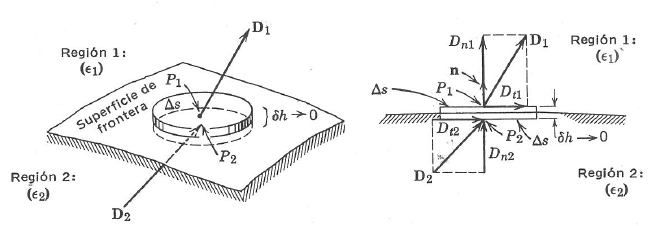
\includegraphics[scale=0.5]{Waves/waves_f5.png}
\end{figure}

Llamando $\mathbf{D}_1$ y $\mathbf{D}_2$ a los campos en puntos dentro de las regiones 










\textbf{SE DEJA PENDIENTE CONTINUAR CON LAS CONDICIONES DE FRONTERA PARA LOS CAMPOS EN MATERIALES JONHK PAG 141}



























































 
\section{Teoría electromagnética para ondas}



El fenómeno electromagnético a nivel macroscópico está descrito por las ecuaciones de Maxwell, publicadas en el año 1873. Su trabajo resumió el estado de la teoría electromagnética y realizó una hipótesis a partir de consideraciones teóricas la existencia de corrientes de desplazamiento eléctrica, lo cual llevó al descubrimiento experimental de Hertz de la propagación electromagnétic. El trabajo de maxwell se basó en una gran cantidad de conocimiento previo empírico y teórico que desarrollaron Gauss, Ampere, Faraday , entre otros. Recordemos, nuevamente, las ecuaciones de Maxwell para los campos eléctrico y magnético.


Volvamos nuevamente a las formas generales de las ecuaciones de Maxwell en su forma diferencial

\begin{eqnarray*}
\nabla \times \mathbf{\mathcal{\bar{E}}} &=& - \frac{\partial \mathcal{\bar{B}}}{\partial t} - \mathcal{\bar{M}} \\
\nabla \times \mathbf{\mathcal{\bar{H}}} &=& \frac{\partial \mathcal{\bar{D}}}{\partial t} + \mathcal{\bar{J}} \\
\nabla \cdot \mathcal{\bar{D}} &=& \rho \\
\nabla \cdot \mathcal{\bar{B}} &=& 0
\end{eqnarray*}

Los campos se describen como sigue

\begin{itemize}
    \item $\mathcal{\bar{E}}$ es el campo eléctrico en voltios por metro (V/m)
    \item $\mathcal{\bar{H}}$ es el campo magnético en amperios por metro (A/m)
    \item $\mathcal{\bar{D}}$ es la densidad de flujo eléctrico, en coulombs por metro cuadrado (C/m2)
    \item $\mathcal{\bar{B}}$ es la densidad de flujo magnético, en webers por metro cuadrado (Wb/m2)
    \item $\mathcal{\bar{N}}$ es una medida ficticia de densidad de corriente magnética, en voltios por metro cuadrado (V/m2)
    \item $\mathcal{\bar{J}}$ Es la densidad de corriente eléctrica, en amperios por metro cuadrado (A/m2)
    \item $\rho$ es la densidad volumétrica de carga eléctrica, en Coulombs por metro cúbico (C/m3)
\end{itemize}

Las fuentes de los campos electromagnéticos son las densidades de corrientes, y de carga (últimas tres de la lista arriba). En el espacio vacío se tiene

\begin{eqnarray*}
\mathcal{\bar{B}} &=& \mu_0 \mathcal{\bar{H}} \\
\mathcal{\bar{D}} &=& \epsilon_0 \mathcal{\bar{E}} 
\end{eqnarray*}

\begin{itemize}
    \item $\mu_0 = 4 \pi \times 10 ^{-7}$ es la permeabilidad magnética del espacio libre, en henrios por metro (H/m)
    \item $\epsilon_0 = 8.854 \times 10^{-125}$ es la permitividad eléctrica del espacio libre, en faradios por metro (F/m) 
\end{itemize}

Volvamos ahiora a las formas integrales de las ecuaciones de Maxwell

\begin{eqnarray*}
\oint_S \mathcal{\bar{D}} \cdot d \bar{s} &=& \int_V \rho \ dv = Q \\
\oint_S \mathcal{\bar{B}} \cdot d \bar{s} &=& 0 \\
\oint_C \mathcal{\bar{E}} \cdot d \bar{l} &=& - \frac{\partial}{\partial t} \int_S \mathcal{\bar{B}} \cdot d \bar{s} - \int_S \mathcal{\bar{M}} \cdot \bar{s} \\
\oint_C \mathcal{\bar{H}} \cdot d \bar{l} &=& \frac{\partial}{\partial t} \int_S \mathcal{\bar{D}} \cdot d \bar{s} + \int_S \mathcal{\bar{J}} \cdot \bar{s} 
\end{eqnarray*}

El campo eléctrico se puede expresar como dependiente del tiempo, armónica y en estado estable; por tal, un campo eléctrico sinusoidal que viaja en la dirección $x$ es 

\begin{eqnarray*}
\mathcal{\bar{E}}(x,y,z,t) = \mathcal{E}_x \hat{x} \cos(\omega t + \phi)  
\end{eqnarray*}

Donde $\mathcal{E}_x$ denota la amplitud del campo. El fasor correspondiente al campo estará dado por

\begin{equation*}
\bar{E}(x,y,z) = \hat{x} \ \mathcal{E}_x \ e^{i \phi} 
\end{equation*}

Se asume una representación de fasores cosenoidal, de modo que 


\begin{equation*}
\mathcal{\bar{E}} (x,y,z,t) = \text{Re} \{ \bar{E}(x,y,z) e^{i \omega t} \}
\end{equation*}


Es importante, al tratar con potencia y energía, tener el cuenta el promedio cuadrático. Teniendo el campo

\begin{equation*}
\mathcal{\bar{E}} = \mathcal{E}_x \cos (\omega t + \phi_x) \hat{x} + \mathcal{E}_y \cos (\omega t + \phi_y) \hat{y} + \mathcal{E}_z \cos (\omega t + \phi_z) \hat{z}
\end{equation*}

El cual tiene la forma fasorial 

\begin{equation*}
\mathcal{\bar{E}} = \mathcal{E}_x e^{i \phi_x} \hat{x} + \mathcal{E}_y e^{i \phi_y} \hat{y} + \mathcal{E}_z e^{i \phi_z} \hat{z}
\end{equation*}

Tiene un valor medio cuadrático de 

\begin{eqnarray*}
|\mathcal{\bar{E}}|_{\text{avg}}^2 &=& \frac{1}{T} \int_0^T \mathcal{\bar{E}} \cdot \mathcal{\bar{E}} \ dt \\
&=& \frac{1}{T} \int_0^T \left(  \mathcal{E}_x^2 \cos^2 (\omega t + \phi_x) + \mathcal{E}_y^2 \cos^2 (\omega t + \phi_y) + \mathcal{E}_z^2 \cos^2 (\omega t + \phi_z) \right) \ dt \\ 
&=& \frac{1}{2} (\mathcal{E}_x^2 + \mathcal{E}_y^2) + \mathcal{E}_z^2)  \\
&=& \frac{1}{2} |\bar{E}|^2 \\
&=& \frac{1}{2} \bar{E} \ \bar{E}^*
\end{eqnarray*}

El valor RMS del campo es

\begin{equation*}
|\bar{E}|_{RMS} = \frac{|\bar{E}|}{\sqrt{2}}
\end{equation*}

Bajo la dependencia del tiempo, las ecuaciones en forma diferencial son

\begin{eqnarray*}
\nabla \times \bar{E} &=& - i \omega \bar{B} - \bar{M} \\
\nabla \times \bar{H} &=& \ i \omega \bar{D} + \bar{J} \\
\nabla \cdot \bar{D} &=& \rho \\
\nabla \cdot \bar{B} &=& 0
\end{eqnarray*}


\subsection{Campos en materiales y las condiciones de frontera}

En un material dieléctrico, cuando se aplica un campo eléctrico, causa la polarización de los átomos o moléculas del material, se crean momentos dipolares que aumentan el flujo de desplazamiento total $\bar{D}$. La polarización adicional se llama $\bar{P}$ y queda el campo como

\begin{equation*}
\bar{D} = \epsilon_0 \bar{E} + \bar{P}
\end{equation*}

Si el medio (material) es lineal, la polarización está relacionada linealmente con el campo aplicado, la constante de proporción se llama susceptibilidad eléctrica, se tiene

\begin{equation*}
\bar{P} = \epsilon_0 \chi_e \bar{E}
\end{equation*}

la susceptibilidad puede ser un número complejo, la ecuación de campo queda como sigue

\begin{eqnarray*}
\bar{D} &=& \epsilon_0 \bar{E} + \epsilon_0 \chi_e \bar{E} \\
\bar{D} &=& \epsilon_0 \bar{E} (1+ \chi_e) \\
\bar{D} &=& \epsilon \bar{E}
\end{eqnarray*}

\begin{equation*}
\epsilon_0(1+ \chi_e) = \epsilon = \epsilon' - i \epsilon''
\end{equation*}

La parte imaginaria de la permitividad del medio es debida a las pérdidas en el medio en forma de calor por el amortiguamiento de los momentos dipolares vibrantes. Esta parte imaginaria debe ser negativa por conservación de la energía. Las pérdidas en el material dieléctrico pueden ser consideradas como equivalentes a las pérdidas en los conductores. En un material con conductividad $\sigma$, existirá en él una densidad de corriente de conducción dada por 

\begin{equation*}
\bar{J} = \sigma \bar{E}
\end{equation*}

La ecuación rotacional de Maxwell

\begin{eqnarray*}
\nabla \times \bar{H} &=& i \omega \bar{D} + \bar{J} \\
&=& i \omega \epsilon \bar{E} +\sigma \bar{E} \\
&=& i \omega \epsilon' \bar{E} + (\omega \epsilon'' + \sigma) \bar{E} \\
&=& i \omega \left( \epsilon' - i \epsilon'' - i \frac{\sigma}{\omega} \bar{E} \right)
\end{eqnarray*}

Donde se ha visto que las pérdidas debidas al amortiguamiento dieléctrico ($\omega \epsilon''$) son indistinguibles de las debidas a la conductividad ($\sigma$). El termino $\omega \epsilon'' + \sigma$ se considera como la conductividad total efectiva.\\

Otra cantidad de interés es la denominada \textit{tangente de pérdida} definida como 

\begin{equation*}
\tan \delta = \frac{\omega \epsilon'' + \sigma}{\omega \epsilon'0}
\end{equation*}

la cual se ve como la relación entre la parte real y la parte imaginaria de la corriente de desplazamiento total. Los materiales de microondas son caracterizados usualmente especificando la permitividad real relativa (constante dieléctrica) $\epsilon_r$, con $\epsilon' = \epsilon_0 \epsilon_r$, y la tangente de pérdida en función de la frecuencia. 

Hasta este momento se ha asumido que el vector de momentos dipolares $\bar{P}$ está en la misma dirección que el campo eléctrico. Para los meteriales con este comportamiento se les conoce como isotrópicos. No todos los materiales son isotrópicos, son denominados anisotrópicos y se caracterizan por tener una relaxión más complicada entre $\bar{D}$ y $\bar{P}$. La relación lineal más general entre estos vectores toma la forma de un tensor de rango 2, el cual se escribe de forma matricial de la siguiente forma:

\begin{equation*}
\left[
\begin{aligned}
    D_x \\
    D_y \\
    D_z
\end{aligned}
\right] = 
\left[
\begin{aligned}
    \epsilon_{xx} && \epsilon_{xy}  && \epsilon_{xz}  \\
    \epsilon_{yx} && \epsilon_{yy}  && \epsilon_{yy}  \\
    \epsilon_{zx} && \epsilon_{zy}  && \epsilon_{zz}  
\end{aligned}
\right]
\left[
\begin{aligned}
    E_x \\
    E_y \\
    E_z
\end{aligned}
\right] = [\epsilon]
\left[
\begin{aligned}
    E_x \\
    E_y \\
    E_z
\end{aligned}
\right]
\end{equation*}

Como ejemplos de materiales anisotrópicos podemos mencionar algunas estructuras cristalinas y gases ionizados. \\

Las mismas relaciones pueden hacerse para los campos magnéticos 

\begin{equation*}
\bar{B} = \mu_0 (1 + \chi_m) \bar{H} = \mu \bar{H}
\end{equation*}

\begin{equation*}
\left[
\begin{aligned}
    B_x \\
    B_y \\
    B_z
\end{aligned}
\right] = 
\left[
\begin{aligned}
    \mu_{xx} && \mu_{xy}  && \mu_{xz}  \\
    \mu_{yx} && \mu_{yy}  && \mu_{yy}  \\
    \mu_{zx} && \mu_{zy}  && \mu_{zz}  
\end{aligned}
\right]
\left[
\begin{aligned}
    H_x \\
    H_y \\
    H_z
\end{aligned}
\right] = [\mu]
\left[
\begin{aligned}
    H_x \\
    H_y \\
    H_z
\end{aligned}
\right]
\end{equation*}

\subsubsection*{Campos en una interfaz material general}


\begin{figure}[H]
    \centering
    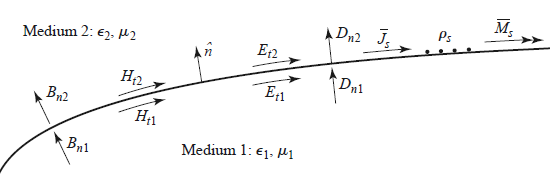
\includegraphics[scale=0.6]{Waves/waves_f6.png}
\end{figure}

Para determinar las condiciones de frontera se hace uso de las formas integrales de las ecuaciones de Maxwell. De esta manera se encuentran las condiciones que deben cumplirse para los campos normales y tangenciales a la interfaz. 

Aplicamos la integral de Maxwell de Gauss en un volumen como se indica en la imagen siguiente

\begin{figure}[H]
    \centering
    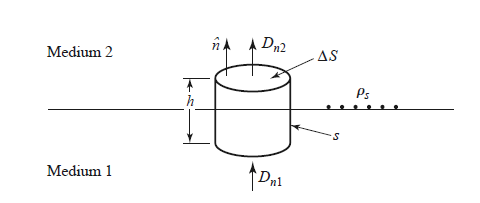
\includegraphics[scale=0.6]{Waves/waves_f7.png}
\end{figure}

\begin{equation*}
\oint_S \bar{D} \cdot d \bar{s} = \int_V \rho \ d v
\end{equation*}

Cuando se hace el límite de $h \to 0$, la contribución tangencial del campo $\bar{D}$ se hace cero, por tanto solamente habrá componente normal sobre el área circular $\Delta S$ por tanto

\begin{equation*}
\left( D_{n2} - D_{n1} \right) \Delta S =  \Delta S \rho_s
\end{equation*}

En el límite, la densidad volumétrica de carga se convierte en densidad superficial. 

\begin{equation*}
D_{n2} - D_{n1} =  \rho_s
\end{equation*}

De manera vectorial se puede escribir

\begin{equation*}
\hat{n} \cdot \left( \bar{D}_{2} - \bar{D}_{1} \right) = \rho_s
\end{equation*}

haciendo una argumentación similar para el campo $B$, se tiene

\begin{equation*}
\hat{n} \cdot \bar{B}_2 = \hat{n} \cdot \bar{B}_1
\end{equation*}

Para la parte tangencial del campo eléctrico, vemos la fórmula integral 

\begin{equation*}
\oint_C \bar{E} \cdot d \Bar{l} = - i \omega \int_S \bar{B} \cdot d \bar{s} - \int_S \bar{M} \cdot d \bar{s}
\end{equation*}

aplicada a la línea cerrada:

\begin{figure}[H]
    \centering
    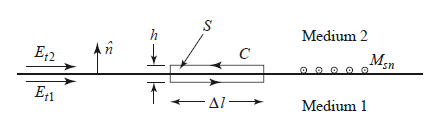
\includegraphics[scale=0.6]{Waves/waves_f8.png}
\end{figure}

nuevamente hacemos e límite $h \to 0$, el área de la superficie $\Delta l \ h$ tiende a cero, por lo que la integral de superficie de $\Bar{B}$ desaparece. Sin embargo, la contribución del campo $\bar{M}$ puede no anularse si en la superficie existe una densidad de corriente superficial magnética: de modo que se puede escribir mediante la función delta de dirac:

\begin{equation*}
\bar{M} = \bar{M}_s \delta (h)
\end{equation*}

por tanto, la ecuación queda

\begin{eqnarray*}
\Delta l E_{t1} - \Delta l E_{t2} &=& - \Delta l M_s \\
 E_{t1} - E_{t2} &=& - M_s
\end{eqnarray*}

o, vectorialmente

\begin{equation*}
\left( \bar{E}_2 - \bar{E}_1 \right) \times \hat{n} = \bar{M}_s
\end{equation*}

De manera similaar para los campos magnéticos

\begin{equation*}
\hat{n} \times \left( \bar{H}_2 - \bar{H}_1 \right) = \bar{J}_s
\end{equation*}

Estas son las expresiones más generales para las condiciones de frontera

\subsubsection*{Campos en la interfaz dieléctrica}

Cuando los materiales son dieléctricos, no existen cargas libres ni corrientes superficiales, por tanto las condiciones de frontera quedarán

\begin{eqnarray*}
\hat{n} \cdot \bar{D_1} &=& \hat{n} \cdot \bar{D_2} \\
\hat{n} \cdot \bar{B_1} &=& \hat{n} \cdot \bar{B_2} \\
\hat{n} \times \bar{E_1} &=& \hat{n} \times \bar{E_1} \\
\hat{n} \times \bar{H_1} &=& \hat{n} \times \bar{H_2} \\
\end{eqnarray*}

\subsubsection*{Campos en la interfaz con un conductor perfecto}

Cuando se tiene un material conductor con una alta conductividad (se puede asumir $\sigma \to \infty$) todos los campos son nulos dentro del material condcutor perfecto. En este tipo de casos se tendrá que las condiciones de frontera son:


\begin{eqnarray*}
\hat{n} \cdot \bar{D} &=& \rho_s \\
\hat{n} \cdot \bar{B} &=& 0 \\
\hat{n} \times \bar{E} &=& 0 \\
\hat{n} \times \bar{H} &=& \bar{J_s}
\end{eqnarray*}

\subsection{Ecuación de onda y soluciones básicas para ondas planas}

en un medio homogéneo, isotrópico, lineal y sin fuentes de campos, la ecuación de maxwel puede llegarse a simlpificar en 

\begin{eqnarray*}
\nabla^2 \bar{E} + \omega^2 \ \mu \epsilon  \bar{E} \\
\nabla^2 \bar{H} + \omega^2 \ \mu \epsilon  \bar{H}
\end{eqnarray*}

Se define la constante de propagación $\beta=\omega \sqrt{\mu \epsilon}$, y se asume la solución, como se mostró en la sección \ref{Ondas_planas_uniformes_en_es_espacio_vacio}, se tiene la solución (para ondas viajantes en la direción x)

\begin{equation*}
E_x(z) = E^+ e^{i \beta z} + E^- e^{-i \beta z}
\end{equation*}

o escrito de otra forma

\begin{equation*}
\mathcal{E} (x,t) = E^+ \cos (\omega t - \beta z) + E^- \cos (\omega t + \beta z)
\end{equation*}

Nuevamente tenemos la velocidad de propagación

\begin{equation*}
v_p = \frac{\omega}{\beta} = \frac{1}{\sqrt{\mu \ \epsilon}}
\end{equation*}

Y también la longitud de onda para las ondas planas

\begin{equation*}
\lambda = \frac{2 \pi}{\beta} = \frac{2 \pi v_p}{\omega } = \frac{v_p}{f}
\end{equation*}

Veamos el campo magnético, que por ecuación de maxwell es

\begin{equation*}
H_y = \frac{i}{\omega \mu} \frac{\partial E_x}{\partial z} = \frac{1}{\eta} (  E^+ e^{-i \beta z} - E^- e^{i \beta z} )
\end{equation*}

donde $\eta = \sqrt{\mu / \epsilon}$ se denomina la impedancia intrínseca del medio.

\subsubsection*{Medio con pérdidas}

Cuando el medio tiene pérdidas, tenemos que hay una conductividad $\sigma$ la ecuación de onda queda

\begin{equation*}
\nabla^2 \bar{E} + \omega^2 \ \mu \epsilon \left( 1 - i \frac{\sigma}{\omega \epsilon} \right) \bar{E} = 0
\end{equation*}

En este caso se tiene que la constante de propagación cambia de ser $\beta^2=\omega^2 \mu \epsilon$ a $\omega^2 \mu \epsilon (1-i(\sigma/\omega \epsilon))$ y se tiene un número complejo de onda o constante compleja de propagación de onda

\begin{equation*}
\gamma = \alpha + i \beta = i \omega \sqrt{\mu \epsilon} \sqrt{1-i \frac{\sigma}{\omega \epsilon}}
\end{equation*}

en este caso se asume una solución para una onda plana en dirección $x$ par que quede la solución

\begin{equation*}
E_x(z) = E^+ e^{-\gamma z} + E^- e^{\gamma z}
\end{equation*}

La onda que viaja en el sentido positivo de $x$ tiene el factor

\begin{eqnarray*}
e^{- \gamma z} = e^{- \alpha z} e ^{-i \beta z}
\end{eqnarray*}
Note que de esta manera el campo se atenúa en el espacio $\alpha$.

El campo magnético en este caso será

\begin{equation*}
H_y = \frac{i}{\omega \mu} \frac{\partial E_x}{\partial z} = \frac{1}{\eta} (  E^+ e^{-i \gamma z} - E^- e^{i \gamma z} )
\end{equation*}

Aquí la impedancia intrínseca del medio está dada por

\begin{equation*}
\eta = \frac{i \omega \mu}{\gamma}
\end{equation*}

\subsubsection*{Medio es un conductor}

Si el medio es un conductor, podemos decir que su conductividad es muy alta, por tanto $\sigma \gg \omega \epsilon$, se puede hacer la aproximación de $\gamma$


\begin{equation*}
\gamma = \alpha + i \beta \approx i \omega \sqrt{\mu \epsilon} \sqrt{ \frac{\sigma}{i \omega \epsilon}} = (1 + i) \sqrt{\frac{\omega \mu \sigma}{2}}
\end{equation*}

\subsection{Solución general de las ondas planas}

veamos la ecuación de Helmholtz para el campo eléctrico en coordenadas rectangulares

\begin{equation*}
\nabla^2 \bar{E} + \beta_0^2 \Bar{E} = \frac{\partial^2 \Bar{E}}{\partial x^2} + \frac{\partial^2 \Bar{E}}{\partial y^2} + \frac{\partial^2 \Bar{E}}{\partial z^2} + \beta_0^2 \Bar{E} = 0
\end{equation*}

Esto da como resultado que para cada coordenada cartesiana

\begin{equation*}
 \frac{\partial^2 E_i}{\partial x^2} + \frac{\partial^2 E_i}{\partial y^2} + \frac{\partial^2 E_i}{\partial z^2} + \beta_0^2 E_i = 0
\end{equation*}

Esta ecuación diferencial parcial puede resolverse mediante el método de separación de variables. Se empieza por asumir que la solución para la componente del campo $E_x$ se puede escribir como el producto de

\begin{equation*}
E_x(x,y,z) = f(x)g(y)h(z)
\end{equation*}

la solución final de la ecuación diferencial estará dada por 

\begin{equation*}
\bar{E} = \bar{E}_0 e^{- i \ \bar{\beta} \cdot \bar{r}}
\end{equation*}

donde tenemos que 

\begin{equation*}
\bar{r} = \hat{x} x + \hat{y} y + \hat{z} z
\end{equation*}

Propiedades importantes de esta solución indican que el vector de las amplitudes del campo deben ser perpendiculares a la dirección en la que se propaga. 

\begin{equation*}
\bar{\beta} \cdot \bar{E}_0 = 0
\end{equation*}


El campo magnético está dado por

\begin{equation*}
\bar{H} = \frac{1}{\eta_0} \hat{n} \times \bar{E}
\end{equation*}

\subsubsection*{Polarización circular de las ondas}

sabemos que las ondas viajan hacia la dirección perpendicular de la amplitud de $\Bar{E}$ y $\bar{H}$. Hasta ahora hemos visto que la orientación del vector $\bar{E}$ no cambia con el tiempo, es decir, siempre es perpendicular a $\hat{x}$, propagándose en la dirección $\hat{z}$. Este tipo de onda plana se considera una \textit{onda de polarización lineal}. Para este caso se tendrá que $\bar{H}$ será perpendicular a $\hat{y}$. \\

Existe una polarización de las ondas planas en las que la dirección del campo $\bar{E}$ también cambia con el tiempo. Esto quiere decir que el vector rota sobre planos $xy$ con una velocidad angular. Como se puede observar en la siguiente imagen

\begin{figure}[H]
    \centering
    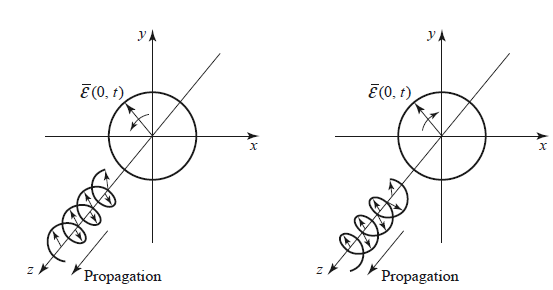
\includegraphics[scale=0.6]{Waves/wave_f9.png}
\end{figure}

\subsection{Potencia y energía}

En general, una fuente de energía electromagnética establece campos que almacenan energía eléctrica y magnética, y transportan potencia que puede transmitirse o disiparse como pérdida. En el caso del estado estacionario sinusoidal, la energía eléctrica almacenada promedio en un volumen V se da por
 \begin{eqnarray*}
W_e &=& \frac{1}{4} \text{Re} \left\{ \int_V \bar{E} \cdot \bar{D}^* \ d v \right\} \\
W_m &=& \frac{1}{4} \text{Re} \left\{ \int_V \bar{H} \cdot \bar{B}^* \ d v \right\} 
 \end{eqnarray*}

Tanto para campos eléctricos como para campos magnéticos. Si el medio es isotrópico, lineal, homogéneo y sin pérdida, entonces la permitividad y permeabildiad son escalares reales y constantes, entonces las energías promedio almacenadas son

\begin{eqnarray*}
W_e &=& \frac{\epsilon}{4} \text{Re} \left\{ \int_V \bar{E} \cdot \bar{E}^* \ d v \right\} \\
W_m &=& \frac{\mu}{4} \text{Re} \left\{ \int_V \bar{H} \cdot \bar{H}^* \ d v \right\} 
 \end{eqnarray*}

 De aqui se puede derivar el teorema de Poynting, el cual lleva a la conservación de energía de campos electromagnéticos y fuentes.

 Partiendo de las ecuacioes diferenciales de maxwell y con algunas propiedades vectoriales, se concluye que

 \begin{equation*}
- \frac{1}{2} \int_V ( \bar{E} \cdot \bar{J}_s + \bar{H} \cdot \bar{M}_s  ) dv = \frac{1}{2} \oint_S \left( \bar{E} \times \bar{H}^* \right) \cdot d \bar{s} + \frac{\sigma}{2} \int_V |\bar{E}|^2 d v + \frac{\omega}{2} \int_V (\epsilon'' |\bar{E}|^2 + \mu'' |\bar{H}|^2) d v + i \frac{\omega}{2}   \int_V (\mu' |\bar{H}|^2 - \epsilon' |\bar{E}|^2) d v
 \end{equation*}


Esta ecuación de balances de potencia es el teorema de Poynting. La integral de la parte izquierda de la ecuación representa la potencia compleja $P_s$ entregada por las fuentes de campo $\bar{J}_s$ y $\bar{M}_s$ dentro del volumen

\begin{equation*}
P_s = - \frac{1}{2} \int_V ( \bar{E} \cdot \bar{J}_s + \bar{H} \cdot \bar{M}_s  ) dv
\end{equation*}

Laprimera integral de la parte derecha de la ecuación representa el flujo de potencia compleja que sale de la superficie cerrada $S$, se define entoncdes el \textit{vector de Poynting} como $\bar{S}$

\begin{equation*}
\bar{S} =  \bar{E} \times \bar{H}^* 
\end{equation*}

por tanto este flujo de potencia se representa

\begin{equation*}
P_o = \frac{1}{2} \oint_S \left( \bar{E} \times \bar{H}^* \right) \cdot d \bar{s} = \frac{1}{2} \oint_S \bar{S} \cdot d \bar{s}
\end{equation*}

Las partes reales de las potencias $P_s$ y $P_o$ representan potencias promedio.

La segunda y tercera integral de la parte derecha de la ecuación son escalares reales que representan la potencia promedio disipada en el volumen $V$ debido a la conductividad y pérdidas dieléctricas y magnéticas. $P_l$

\begin{equation*}
P_l =  \frac{\sigma}{2} \int_V |\bar{E}|^2 d v + \frac{\omega}{2} \int_V (\epsilon'' |\bar{E}|^2 + \mu'' |\bar{H}|^2) d v 
\end{equation*}

Esta se denomina en algunas ocasiones como la ley de Joule. La última integral finalmente está relacionada con las energías electromagnéticas almacenadas, son potencias reactivas.

El teorema de Poynting se escribe nuevamente como sigue

\begin{equation*}
P_s = P_o + P_l + 2 i omega (W_e - W_e)
\end{equation*}

La potencia total entregada por las fuentes de ondas es la suma de la potencia transmitida a través de la superficie más la potencia disipada por pérdidas térmicas y electromagnéticas, más $2 \omega$ veces la potencia reactiva neta que se almacena en el volumen.

\subsubsection*{Potencia absorbida por un buen conductor}


En la vida practica las líneas de transmisión involucran conductores imperfectos, dando lugar a pérdidas de atenuación de campo y de potencia, así como generación de ruido. Para calcular estas pérdidas es necesario que se calcule la potencia disipada por estos conductores. Considere la siguiente geometría

\begin{figure}[H]
    \centering
    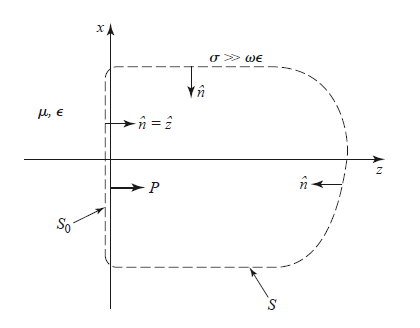
\includegraphics[]{Waves/waves_f10.png}
\end{figure}

Representando la interfaz de un medio sin pérdidas y un conductor bueno. Un campo es incidente en la dirección $z<0$ y penetra en el conductor en $z>0$. La potencia real promedio que entra a la sección de volumen $V$ del conductor definida por el área transversal $S_0$ en la interfaz y el área $S$ dentro del conductor es 

\begin{equation*}
P_{avg} = \frac{1}{2} \text{Re} \int_{S_0+S} \bar{E} \times \bar{H}^* \cdot \hat{n} d s
\end{equation*}

Dado que las ondas son planas, van en dirección $\hat{z}$; además, el rápido decaimiento de los campos dentro de un material conductor también da lugar a que la contriución de estos en la región $S$ sea despreciable. Esto deja como resultado que la potencia sea

\begin{equation*}
P_{avg} = \frac{1}{2} \text{Re} \int_{S_0} \bar{E} \times \bar{H}^* \cdot \hat{z} d s
\end{equation*}

simplificamos

\begin{eqnarray*}
\hat{z} \cdot (\bar{E} \times \bar{H}^*) &=& (\hat{z} \times \bar{E}) \cdot  \bar{H}^* \\
&=& \eta \bar{H} \cdot  \bar{H}^* 
\end{eqnarray*}

Si $R_s = \text{Re} \eta = \sqrt{\frac{\omega \mu}{2 \sigma}}$, la potencia queda

\begin{equation*}
P_{avg} = \frac{1}{2} \frac{R_s}{2} \int_{S0} |\bar{H}|^2 \ ds
\end{equation*}

$R_s$ se define como la resistencia de superficie del conductor

\subsection{Reflexión de ondas planas de una interfaz de medios}

Cuando una onda plana de campo eléctrico pasa del espacio libre a un medio con $\epsilon$, $\mu$ y $\sigma$, parte de la onda se transmitirá al materia, y otra parte se refleja en la dirección opuesta:

\begin{figure}[H]
    \centering
    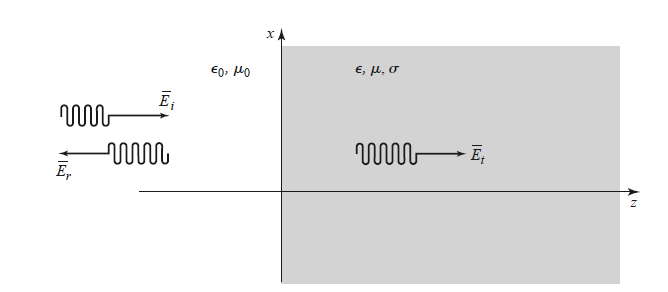
\includegraphics[scale=0.6]{Waves/waves_f11.png}
\end{figure}

Los campos incidentes son

\begin{eqnarray*}
\bar{E}_i &=& \hat{x} E_0 e^{- i \beta_0 z} \\
\bar{H}_i &=& \hat{y} \frac{1}{\eta_0} E_0 e^{- i \beta_0 z}
\end{eqnarray*}

Con amplitud $E_0$ arbitraria.

Las ondas reflejadas son 

\begin{eqnarray*}
\bar{E}_r &=& \hat{x} \Gamma E_0 e^{+ i \beta_0 z} \\
\bar{H}_r &=& - \hat{y} \frac{1}{\eta_0} \Gamma E_0 e^{+ i \beta_0 z}
\end{eqnarray*}

donde $\Gamma$ se denomina el \textbf{coeficiente de refexión} de la interfaz o medio. El signo positivo de la exponencial es un indicador de la dirección de propagación de la onda hacia $z$ negativo. \\

Los campos transmitidos al material están dados por

\begin{eqnarray*}
\bar{E}_t &=& \hat{x} \ T \ E_0 \ e^{- \gamma z} \\
\bar{H}_t &=& \hat{y} \ \frac{1}{\eta} T \ E_0 \ e^{-\gamma z}
\end{eqnarray*}

donde la constante de propagación es 

\begin{equation*}
\gamma = \alpha + i \beta = i \omega \sqrt{\mu \epsilon} \sqrt{1- i \sigma / \omega \epsilon}
\end{equation*}

y la impedancia del medio es

\begin{equation*}
\eta = \frac{i \omega \mu}{\gamma}
\end{equation*}

En este caso se tiene un problema de frontera, se tiene que los campos son continuos en la interfaz de los materiales, por tanto se tiene como condición de frontera

\begin{eqnarray*}
1 + \Gamma = T \\
\frac{1 - \Gamma}{\eta_0} = \frac{T}{\eta}
\end{eqnarray*}

La solución de el sistema es

\begin{eqnarray*}
\Gamma = \frac{\eta - \eta_0}{\eta + \eta_0} \\
T = \frac{2\eta}{\eta + \eta_0}
\end{eqnarray*}

Examinamos ahora las diferentes posibilidades para el material

\subsubsection*{Medio sin pérdidas}

Si el material es sin pérdidas, esto significa que $\sigma=0$ y que $\epsilon$ y $\mu$ son reales. Entonces la constante de propagación es imaginaria y está dada por 

\begin{equation*}
\gamma = i \beta = i \omega \sqrt{\epsilon \mu} = i \ \beta_0 \sqrt{\epsilon_r \mu_r}
\end{equation*}

La longitud de onda en el material es

\begin{equation*}
\lambda = \frac{2 \pi}{\beta} = \frac{2 \pi}{\omega \sqrt{\epsilon \mu}} = \frac{\lambda_0}{\sqrt{\epsilon_r \mu_r}}
\end{equation*}

la velocidad de fase (o de propagación= es 

\begin{equation*}
v_p = \frac{1}{ \sqrt{\epsilon \mu}} = \frac{c}{ \sqrt{\epsilon_r \mu_r}}
\end{equation*}

 Y la impedancia intrínseca del material será


\begin{equation*}
\eta = \sqrt{\frac{\mu}{\epsilon}} = \eta_0 \sqrt{\frac{\mu_r}{\epsilon_r}}
\end{equation*}

El vector de Poyting en la aregión $z<0$ es

\begin{eqnarray*}
\bar{S}^{-} = \bar{E} \times \bar{H}^* = (\bar{E}_i+\bar{E}_r) \times (\bar{H}_i+\bar{H}_r)^*
\end{eqnarray*}

Que conlleva a 

\begin{equation*}
\bar{S}^{-} = \hat{z} \ |E_0|^2 \frac{1}{\eta_0} \left(1-|\Gamma|^2 + 2 i \ \Gamma \sin (2 \beta_0 z)\right)
\end{equation*}

Dado $\Gamma \in \mathbb{R}$

ahora, para $z >0$, el vector de Poynting es

\begin{equation*}
\bar{S}^{+} = \bar{E}_t \times \bar{H_t}^* = \hat{z} \ \frac{|E_0|^2 \ |T|^2}{\eta}
\end{equation*}

esto puede reescribirse como

\begin{equation*}
\bar{S}^{+} = \hat{z} \ |E_0|^2 \ \frac{1}{\eta_0} \left(1-|\Gamma|^2 \right)
\end{equation*}

Ahora, note que los vectores deben ser iguales en la interfaz $\bar{S}^{+} = \bar{S}^{-}$ en $z=0$. La potencia real promedio en $z<0$ es

\begin{equation*}
P^{-} = \frac{1}{2} \text{Re} \left\{  \bar{S}^- \cdot \hat{z} \right\} = \frac{1}{2} \ |E_0|^2 \frac{1}{\eta_0} \left(1-|\Gamma|^2 \right) 
\end{equation*}

y en $z>0$ es

\begin{equation*}
P^{+} = \frac{1}{2} \text{Re} \left\{  \bar{S}^+ \cdot \hat{z} \right\} = \frac{1}{2} \ |E_0|^2 \frac{1}{\eta_0} \left(1-|\Gamma|^2 \right) = P^{-}
\end{equation*}

\subsubsection*{Medio conductor}

Aquí tenemos las siguientes propiedades

\begin{equation*}
\gamma = (1+i)\sqrt{\frac{\omega \ \mu \ \sigma}{2}} = (1+i) \frac{1}{\delta_s}
\end{equation*}

La impedancia intrínseca es 

\begin{equation*}
\eta =  (1+i)\sqrt{\frac{\omega \ \mu }{2\ \sigma}} = (1+i) \frac{1}{\sigma \ \delta_s}
\end{equation*}

El vector de poynting en $z=0$ es

\begin{equation*}
\bar{S}^{-}(z=0) = \hat{z} \ |E_0|^2 \frac{1}{\eta_0} \left( 1 - |\Gamma|^2 + \Gamma - \Gamma^{*} \right)
\end{equation*}

y para $z>0$

\begin{equation*}
\bar{S}^{+} = \hat{z} \ |E_0|^2 \frac{1}{\eta_0} \left( 1 - |\Gamma|^2 + \Gamma - \Gamma^{*} \right) e^{-2 \alpha z}
\end{equation*}

Las potencias reales promedio son

\begin{eqnarray*}
P^- &=& \frac{1}{2} \ |E_0|^2 \frac{1}{\eta_0} \left( 1 - |\Gamma|^2 +  \right) \\
P^+ &=& \frac{1}{2} \ |E_0|^2 \frac{1}{\eta_0} \left( 1 - |\Gamma|^2 +  \right) e^{-2 \alpha z}
\end{eqnarray*}

La densidad de corriente resultante en la reegión conductora está dada por 

\begin{equation*}
\bar{J}_t = \sigma \bar{E}_t = \hat{x} \sigma \ E_0 T e{- \gamma z} \text{A/m}^2
\end{equation*}

Y la potencia promedio real disipada o transmitida dentro de un volumen de sección transversal de $1\text{m}^2$ es

\begin{equation*}
P^t = \frac{\sigma \ |E_0|^2 \ |T|^2}{4 \ \alpha}
\end{equation*}

\subsubsection*{Conductor perfecto}

Ahora para un conductor perfecto se tiene que $\sigma \to \infty$, $\alpha \to \infty$, $\eta = 0$, $\delta_s \to 0$, $T \to 0$ y $\Gamma \to -1$  y se tiene que los campos decain infinitamente rápido en $z>0$, los campos fuera del conductor son

\begin{eqnarray*}
\bar{E} = \bar{E}_i + \bar{E}_r = - \hat{x} 2 \ i E_0 \sin (\beta_0 z) \\
\bar{H} = \bar{H}_i + \bar{H}_r = \hat{y} \frac{2}{\eta_0} E_0 \cos (\beta_0 z) \\
\end{eqnarray*}

El vector de Poynting es

\begin{equation*}
\bar{S}^- = -\hat{z} \ i \ \frac{4}{\eta_0} |E_0|^2 \sin (\beta_0 z) \cos (\beta_0 z)
\end{equation*}

La cual es puramente imaginaria y significa que no hay potencia entregada a un conductor perfecto. La corriente superficial se reduce a una densidad infinitesimalmente delgada 

\begin{equation*}
\bar{J}_s = \hat{x} \frac{2}{\eta_0} E_0
\end{equation*}


\section{Teoría de líneas de transmisión}



% \chapter{MQTT}

\section{Resumen sobre publicaciones de mensajes y suscripciones de mqtt}

MQTT (del inglés Message Queuing Telemetry Transport) es una arquitectura de publicación suscripción que fue desarrollada primordialmente para conectar dispositivos con limitaciones de ancho de banda y energía a través de comunicaciones inalámbricas. Se trata de un protocolo sencillo y ligero que puede ser ejecutado sobre un socket TCP/IP, un WebSocket, y SSL. \\

MQTT cuenta con dos componentes: 

\begin{itemize}
    \item MQTT broker - Un broker es un punto central de la comunicación. Es el responsable de despachar todos los mensajes entre los clientes
    \item MQTT client - Un cliente es cualquier dispositivo que se conecta al broker. Un cliente que envía mensajes es un cliente publicador. El cliente que recibe el mensaje es un suscriptor. Para que un cliente pueda recibir un mensaje, este debe estar suscrito al Asunto (topic) del mensaje.
\end{itemize}

\subsection{el Asunto}
El asunto o tópico de un mensaje el identificador utilizado por el broker para identificar a los clientes correctos a la hora de entregar los mensajes. Cada cliente que quiera enviar un mensaje, lo publica en su respectivo Asunto, y cada cliente que esté suscrito a dicho Asunto, puede recibir este mensaje. El Asunto es una variable del tipo String, y puede consistir de uno o más niveles de Asunto. Cada nivel está separado por una barra /, por ejemplo \texttt{home/livingroom/temperature}. El Asunto tiene que tener al menos un caracter, y puede diferenciarse por mayúsculas. 

\subsection{Comodines de los asuntos}

Los comodines son caracteres especiales en un asunto que se usa por los cloentes para suscribirse a múltiples Asuntos. MQTT soporta comodines de un nivel y multinivel.

\begin{itemize}
    \item Un comodin de un nivel está representado por el signo (+). Para que un cliente reciba mensajes, todos los niveles del Asunto suscrito, excepto el nivel con el signo (+), deben coincidir con el Asunto del mensaje entrante. Como ejemplo, si un cliente se susvribe a \texttt{home/floor1/+/temperature}, entonces, dicho cliente podrá recibir mensajes que se publiquen a los Asuntos \texttt{home/floor1/livingroom/temperature}, \texttt{home/floor1/kitchen/temperature}
    \item Para los comodines multinivel, se usa el caracter \#; representa un reemplazo en el nivel y todos los subniveles. Como ejemplo, un cliente suscrito a \texttt{home/floor1/ \#}, podrá recibir mensajes que se publiquen en \texttt{home/floor1/kitchen/temperature}, \texttt{home/floor1/kitchen/temperature/sensor3}, \texttt{home/floor1/hall/camera2/movementSensor}, etc. 
\end{itemize}
% \chapter{Sistemas operativos en tiempo real y FreeRTOS}


\section{FreeRTOS}
\subsection{Introducción}

\subsubsection{Qué es un sistema operativo en tiempo real}

Para poder entender con mayor completitud lo que significa un sistema operativo en tiempo real, es importante tener claro qué son en principio los sistemas operativos en sí. Y luego entrar a especificar detalles o conceptos como tiempo real y demás.

\subsubsection{Sistema operativo}

Un sistema operativo es un programa de computadora que soporta las funciones básicas de un computador, y proporciona servicios básicos a otros programas o aplicaciones que son los que se ejecutan en la computadora. Las aplicaciones son las que proporcionan las funcionalidades que el usuario requiere o necesita. Los servicios proporcionados por el sistema operativo hacen que escribir las aplicaciones sea más rápido, más simple y más fácil de mantener.\\

Una aplicación como por ejemplo navegador web, provee las funcionalidades para leer correos, visitar páginas, etc. Este navegador en sí mismo está siendo ejecutado dentro de un entorno que es el que el sistema operativo proporciona.

\subsubsection{Qué es un RTOS}

La mayoría de sistemas operativos permiten la ejecución de varios programas al mismo tiempo. La llamada multi tarea (multitasking). En realidad, cada núcleo del procesador puede estar ejecutando un solo hilo de procesamiento al tiempo. Un elemento del sistema operativo llamado planificador (scheduler) es el responsable de decidir cuál programa se ejecuta y cuándo se ejecuta, y proporciona la sensación de de ejecución simultánea mediante cambios en los programas.\\

El tipo de sistema operativo se define por cómo hace el planificador para decidir cuál programa se ejecuta y cuándo se ejecuta. \\

El planificador de un sistema operativo en tiempo real está diseñado para proveer un patrón de ejecución predecible o normalmente descrito como determinista. Esto es de particular interés en para los sistemas embebidos ya que estos generalmente tienen requerimientos de tiempo real. Un requerimiento de tiempo real es aquel que especifica que un sistema embebido debe responder a cierto evento dentro de un tiempo estrictamente definido (este se conoce como 'deadline'). La garantía total del cumplimiento del requerimiento de tiempo real solamente se puede dar si el comportamiento del planificador del sistema operativo puede ser predicho (en otras palabras que sea determinista).

Los planificadores tradicionales de los sistemas operativos en tiempo real (como el del sistema operativo FreeRTOS, cumple con el requisito de determinismo gracias a que permite al usuario asignar cierta prioridad a cada hilo de ejecución. El planificador hace uso de estas prioridades para conocer cuál es el siguiente hilo que se va a ejecutar. En FreeRTOS un hilo de ejecución se llama tarea o 'task'.\\

\subsubsection{Qué es FreeRTOS}

Es un tipo de sistema operativo en tiempo real diseñado para ser lo suficientemente pequeño para poder ser ejecutado en un microcontrolador. Aunque no está estrictamente limitado a uso exclusivo en MCU. \\

Un MCU es pequeño y restringido en recursos; típicamente el programa es ejecutado desde la ROM. Los MCU son utilizados en sistemas profundamente embebidos, estas son aplicaciones en las que realmente no se ve el procesador como tal o el software que se está ejecutando. Normalmente tienen un trabajo especifico, especializado y dedicado para hacer. Las restricciones de tamaño y naturaleza dedicada de aplicación raramente justifican el uso de una implementación completa de FreeRTOS. De hecho hace que sea posible la implementación total de un RTOS. El sistema FreeRTOS proporciona por tanto la funcionalidad de planificación en tiempo real del núcleo, intercomunicación de tareas, temporización y sincronización. 



\subsection{Fundamentos de RTOS}

En esta sección se realiza una breve introducción a los conceptos de multi tarea en tiempo real.

\subsubsection{Multitasking}

El \textbf{kernel} es el componente central dentro de un sistema operativo. Los sistemas operativos como Linux emplean kernels que permiten a los usuarios acceder al computador de manera aparentemente simultáneamente. Múltiples usuarios pueden ejecutar varios programas aparentemente concurrentemente. \\

Cada programa en ejecución es una tarea o \textbf{task} bajo el control del sistema operativo. Si un OS puede ejecutar múltiples tareas de esta forma, se denomina \textbf{multitasking}.\\

El uso de un SO multitasking puede simplificar el diseño de lo que podría ser una aplicación bastante más complicada de otra manera:

\begin{itemize}
    \item El multitasking y la comunicacion entre tasks permiten a una aplicación compleja ser separada en un conjunto de tareas más pequeñas y más manejables.
    \item La partición de tareas puede resultar en pruebas de software más sencillas de realizar, y en reutilización de código.
    \item Se pueden eliminar detalles complejos de temporización y secuenciación del código de la aplicación y convertirse en una responsabilidad del sistema operativo.
\end{itemize}

\paragraph{Multitasking vs concurrencia}

Un procesador convencional puede ejecutar solamente una tarea al tiempo, pero intercambiando rápidamente entre tareas, un sistema multitasking puede dar la apariencia de estar ejecutando varias tareas de manera concurrida. Esto se representa en el diagrama siguiente. Este diagrama muestra el patrón de ejecución de tres tareas con respecto al tiempo. 

\begin{figure}[H]
    \centering
    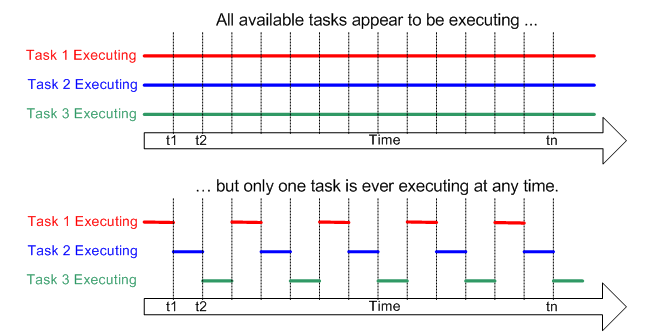
\includegraphics[scale=0.7]{RTOS/f1.PNG}
\end{figure}

\subsubsection{Planificación}

El planificador es la parte del kernel responsable de decidir cuál es la tarea que se ejecuta en cualquier tiempo específico. El kernel puede suspender y más adelante reanudar cualquier tarea muchas veces durante el tiempo de vida de la tarea.\\

La política de planificación es el algoritmo utilizado por el planificador para tomar la decisión de cuál es la tarea que se ejecutará en cualquier punto del tiempo. La política de planificación de un sistema multi usuario en tiempo no real lo más probable es que permita a cada tarea una proporción "justa" del tiempo de provesamiento. \\

Adicionalmente a ser suspendido por el kernel de manera involuntaria, una tarea puede escoger suspenderse a sí misma. Esto lo hará si necesita retardar (\textbf{sleep}) un periodo fijado de tiempo o esperar (\textbf{block}) para que algún recurso se vuelva disponible (por ejemplo un puerto serial) o que algún evento ocurra (por ejemplo una señal proveniente). Una tarea bloqueada o dormida no puede ejecutarse y no tomara parte de tiempo de procesamiento.  

\begin{figure}[H]
    \centering
    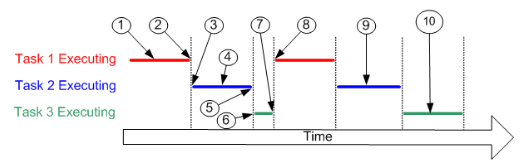
\includegraphics[scale=1]{RTOS/f2.PNG}
\end{figure}

los tiempos marcado en la imagen anterior son:

\begin{itemize}
    \item En (1) se ejecuta la tarea 1.
    \item En (2) el kernel suspende (intercambia) la tarea 1.
    \item Y el el mismo tiempo continúa la tarea 2.
    \item Mientra se ejecuta la tarea 2 en el tiempo (4) bloquea los periféricos del procesador para su acceso exclusivo.
    \item en (5) y (6) se suspende tarea 2 y reanuda tarea 3.
    \item La tarea 3 trata de usar recursos de periféricos, al ver que no está disponible, se suspende en el tiempo (7).
    \item En el tiempo (8) se reanuda tarea 1.
    \item En el tiempo (9) la tarea 2 finaliza el uso del periférico y entonces lo desbloquea.
    \item En (10) la tarea 3 ya encuentra disponibilidad de periféricos y puede ejecutarse.
\end{itemize}

\subsubsection{Cambio de contexto}

Al ejecutarse una tarea esta utiliza recursos del procesador o microcontrolador tales como registros y accede a la memoria RAM y ROM de igual manera que cualquier otro programa. Estos recursos comprenden el \textbf{contexto} de la ejecución de la tarea.

Una tarea es una porción de código secuencial, este no sabe cuándo será suspendido (o intercambiado por otra tarea) o reanudado por el kernel; incluso no sabe si estas suspensiones o reanudaciones ocurrieron. Considerando un ejemplo en que una tarea es suspendida por el kernel justamente antes de ejecutar una instrucción que realiza la suma de los valores de dos registros del procesador. Mientras la tarea está suspendida otras son ejecutadas y pueden modificar los valores contenidos en estos registros. Tras la reanudación de la tarea, esta no sabrá que los valores de los registros fueron cambiados. Es importante tener esto en cuenta porque si la tarea asume que los valores no se cambiaron, el valor de la suma no será correcto. \\

Para prevenir este tipo de posibles errores es esencial que al reanudarse una tarea tenga un contexto idéntico al que tenía antes de ser suspendido. El kernel del sistema operativo es el responsable de asegurar estas condiciones y lo realiza guardando el contexto de la tarea antes de suspenderla. Una vez se reanuda, este contexto se restaura por el sistema operativo. Este proceso de guardar y cargar el contexto de cada tarea se llama intercambio de contexto.

\subsubsection{Aplicaciones de Tiempo Real}

Los Sistemas Operativos en Tiempo Real logran ser multi-tarea a través de los anteriores principios, pero sus objetivos son muy diferentes a aquellos que no son tiempo real. El objetivo diferente se refleja en la política de planificación. Los sistemas embebidos y de tiempo real están diseñados para proporcionar una respuesta oportuna a eventos del mundo real. Estos eventos del mundo real pueden tener tiempos de terminación antes de los cuales el sistema embebido debe responder y la política de planificación RTOS tiene que asegurar que estos plazos o tiempos de terminación se cumplan. \\

Para lograr lo anterior el diseñador(a) de software le debe asignar un nivel de prioridad a cada tarea. La política de planificación del RTOS se asegura entonces de que la tarea con más alta prioridad se pueda ejecutar en el tiempo de procesamiento de la tarea dado. Esto puede requerir que se comparta tiempo de procesamiento "equitativo" entre tareas que tengan misma prioridad si ambas están listas para ejecutarse.

\paragraph{Ejemplo} El ejemplo más básico de RTOS es un sistema que incorpora un teclado y un LCD. Un usuario debe tener retroalimentación visual de cada tecla presionada dentro de un periodo de tiempo razonable. Si el usuario no puede ver que la tecla presionada ha sido aceptada dentro de este tiempo, el software será, en el mejor de los casos, incómodo de usar. Si el tiempo máximo aceptable era de 100ms, cualquier respuesta que esté por debajo de este tiempo será considerado como aceptable. Esta funcionalidad puede ser implementada como una tarea autónoma con la siguiente estructura.

\begin{verbatim}
    void vKeyHandlerTask( void *pvParameters )
    {
    // Key handling is a continous process and as such the task \\
    // is implemented using an infinite loop (as
    // most real time tasks are) \\
    for( ;; )
    {
        [suspend waiting for a press key]
        [process the key press]
    }
    }
\end{verbatim}

Ahora asúmase que el sistema en tiempo real también está llevando a cabo una unción de control que se basa en una entrada digital filtrada. Esta entrada debe ser muestreada, filtrada, y el ciclo de control ejecutado cada 2ms. Para una correcta operación de filtro, la regularidad temporal de la muestra debe ser precisada a 2.5ms. Esta funcionalidad debe ser implementada como una tarea autónoma con una estructura similar a la anterior: \\

\begin{verbatim}
    void vControlTask( void *pvParameters )
    {
        for( ;; )
    {
        [suspend waiting for 2ms since the start of the previous cycle]
        [sample the input]
        [filter the signal]
        [perform control algorithm]
        [output result]
    }
    }
\end{verbatim}

El diseñador de software debe asignar a la tarea de control una prioridad mayor ya que:

\begin{enumerate}
    \item El plazo de tiempo para la tarea de control es más estricta que la de la lectura de tecla.
    \item La consecuencia de no cumplir el plazo de tiempo es mayor para la tarea de control que para la otra.
\end{enumerate}

\subsubsection{Planificación de tareas}

\begin{figure}[H]
    \centering
    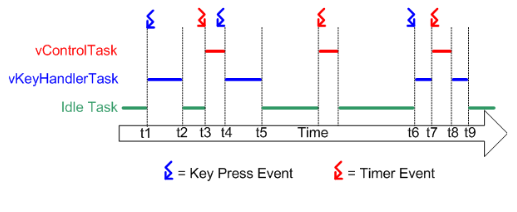
\includegraphics[scale=1]{RTOS/f3.PNG}
\end{figure}

El diagrama muestra cómo deberían ser planificadas las tareas por el sistema de tiempo real. El RTOS crea por sí mismo una tarea llamada \textbf{idle} task (tarea de inactividad) la cual se ejecuta solamente cuando no hay ninguna otra tarea ejecutándose o disponibles. Esta tarea siempre está en un estado en el que puede ejecutarse. \\

\begin{itemize}
    \item Al inicio ninguna de las dos tareas se está ejecutando ni están disponibles para ejecución, por ello la tarea actual es \textbf{idle}. Pues vControlTask está esperando para el momento correcto de arranque de un nuevo ciclo de lectura y vKeyHandlerTask está esperando a que se oprima una tecla.
    \item En t1 se presiona una tecla. vKeyHandlerTask ahora está disponible para ejecutarse, tiene una prioridad mayor que \textbf{idle} task. 
    \item en t2 vKeyHandlerTask completa su proceso de tecla y visualización en LCD. No puede continuar hasta que sea presionada otra tecla, así que se auto suspende y se reanuda la tarea inactiva. 
    \item En t3 un evento de temporización indica que es tiempo de ejecutarse el siguiente ciclo de control. vControlTask ahora está disponible y como tiene la mayor prioridad entonces el planificador da el tiempo de ejecución de procesamiento.
    \item Entre t3 y t4, mientras vControlTask se está ejecutando, se presiona una tecla. Eso significa que vKeyHandlerTask pasa a estar disponible para ejecución, pero como tiene un nivel de prioridad menor, entonces no se le asigna un tiempo de procesamiento por el planificador.
    \item En t4 el proceso de control termina su ejecución y no puede reiniciar hasta el siguiente evento de temporización; por tanto se suspende a sí mismo. vKeyHandlerTask ahora es la tarea con la mayor prioridad disponible para ejecutarse, por ende el planificador le da tiempo de procesamiento e inicia su ejecución. 
    \item En t5 se termina el proceso de la tecla y vKeyHandlerTask se suspende para esperar siguiente evento. No hay tareas así que se ejecuta 'inactiva'
    \item En el tiempo t6 se presiona otra tecla, pero en medio del procesamiento de la tarea, el evento de temporización de control se dispara, entonces por sus prioridades indican, el planificador le da tiempo de procesamiento a vControlTask y suspende vKeyHandlerTask guardando su contexto para poder seguir siendo ejecutado después.
\end{itemize}

\subsection{Implementación de RTOS}

Esta sección describe el código fuente de intercambio de contextos de un RTOS desde el inicio. En este ejemplo se utiliza el MCU Atmel AVR con el puerto de FreeRTOS. La sección finaliza con un vistazo muy detallado paso por paso de un cambio de contextos completo.

\subsubsection{Tipos de datos}

Cada puerto FreeRTOS tiene un único archivo cabecera \texttt{portmacro.h} el cual contiene (entre varias otras cosas) definiciones de dos tipos de variables específicos: \texttt{TickType\_t} y \texttt{BaseType\_t}.

\paragraph{\texttt{TickType\_t}}

El sistema operativo siempre configura una interrupción periódica, se conoce con el nombre de interrupción de tick. El número de interrupciones de tick que han ocurrido desde que el sistema RTOS inicia se llama contador de tick. Este contador se utiliza como una medida de tiempo. El tiempo entre una interrupción de tick y la siguiente se denomina periodo de tick. Y los tiempos se especifican como múltiples periodos de tick.\\

\texttt{TickType\_t} es el tipo de dato utilizado para contener el valor de conteo de ticks y para especificar tiempos. Este tipo de dato puede ser de 16 bits sin signo o de 32 bits sin signo, dependiendo del parámetro de configuración de \texttt{configUSE\_16\_BIT\_TICKS} en \texttt{FreeRTOSConfig.h}; si su valor es 1, entonces \texttt{TickType\_t} es un \texttt{uint16\_t}, si el valor es 0 entonces será \texttt{uint32\_t}.

\paragraph{\texttt{BaseType\_t}}

Este siempre se define como el tipo de dato más eficiente para la arquitectura. Típicamente es un dato de 32 bits, y si la arquitectura es menor, entonces será de este tamaño. \texttt{BaseType\_t} se usa generalmente para retornar tipos de datos que solamente puede tomar un rango muy limitado de valores, y valores booleanos \texttt{pdTRUE/pdFALSE}.\\

Algunos compiladores.

\paragraph{Nombres de funciones}

Lasfunciones tienen diferenes prefijos y cada uno indica el tipo de dato de retorno, y el archivo sobre el que está definido. Por ejemplo

\begin{itemize}
    \item \texttt{vTaskPrioritySet()}: la 'v' indica que retorna un \texttt{void} y está definido dentro de \textbf{task.c}.
    \item \texttt{xQueueReceive()}: la 'x' indica que el retorno es del tipo \texttt{BaseType\_t} y está definido dentro de \textbf{queue.c}.
    \item \texttt{pvTimerGetTimerID()} la 'p' y la 'v' indican que el retorno es un puntero a un \texttt{void} y está definido dentro de \textbf{timers.c}
\end{itemize}

Funciones privadas en un entorno tienen el prefijo 'prv'.

\paragraph{Nombres de macro}

La mayoría de los macros están escritos en mayúsculas y tienen prefijos con letras minúsculas que indican dónde está definido dicho macro. 

\begin{itemize}
    \item \texttt{portMAX\_DELAY)} es un macro que está definido en \texttt{portable.h} o en \texttt{portmacro.h}.
    \item \texttt{taskENTER\_CRITICAL()} está definido en \texttt{task.h}.
    \item \texttt{pdTRUE} en \texttt{projdefs.h}.
    \item \texttt{configUSE\_PREEMPTION)} en \texttt{FreeRTOSConfig.h}
    \item \texttt{errQUEUE\_FULL)} en \texttt{projdefs.h}.
\end{itemize}

Note que las funciones API de los semáforos están escritas casi enteramente como un conjunto de macros, aunque siguen la convención de nombres de funciones. 

\subsubsection{Piezas de armado}

\paragraph{Herramientas de desarrollo}

Un objetivo de FreeRTOS es que sea simple y sencillo de entender. Para este fin la mayoría de códigos fuente de sistemas operativos en tiempo real están escritos en C. \\

El ejemplo presentado en esta sección utiliza una herramienta de desarrollo para windows de AVR.

\paragraph{El tick de RTOS}

Cuando está en modo inactivo (sleeping) una tarea de tiempo real va a especificar un tiempo después del cual requerirá 'despertar'. Cuando está bloqueado, la tarea puede especificar un tiempo máximo el cual desea esperar.\\

El kernel de FreeRTOS mide el tiempo en unidades básicas llamadas \textbf{ticks}. Una interrupción de tiempo (tick interrupt) incrementa el conteo de ticks con una estricta precisión del tiempo. Permitiendo al kernel medir el tiempo con una resolución de la frecuencia de la interrupción. \\

Cada vez que el contador de ticks incrementa el kernel del sistema operativo debe evaluar y ver si es momento de desbloquear o despertar una tarea. Es posible que una tarea despertada o desbloqueada durante el tick ISR tenga una prioridad más alta que aquella relacionada con la tarea interrumpida. Si este es el caso el tick ISR deberá retornar a la tarea recien despertada o desbloqueada, interrumpiendo efectivamente una tarea pero regresando a otra.


\begin{figure}[H]
    \centering
    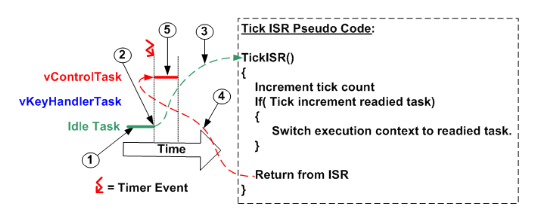
\includegraphics[scale=1]{RTOS/f4.PNG}
\end{figure}

\begin{itemize}
    \item En (1) se está ejecutanto la tarea inactiva de RTOS.
    \item En (2) ocurre un tick de RTOS (evento o interrupción) y el control transfiere al ISR (3).
    \item El ISR de la interrupción por temporización hace que vControlTask esté lista para ejecutarse, y como esta tarea tiene mayor prioridad que la inactiva, se hace el cambio de contexto al de vControlTask.
    \item Como el contexto de ejecución ahora es el de la tarea vControlTask, saliendo del ISR (4) retorna el control a vControlTask, el cual empieza a ejecutarse.
\end{itemize}

Un cambio de contexto de ejecución que ocurre de esta manera se denomina preventiva \textbf{preemptive} ya que la tarea interrumpida es cambiada pero sin suspenderse voluntariamente.

El puerto AVR de FreeRTOS utiliza un evento de comparación en un temporizador para generar el tick.

\paragraph{Atributos de señal GCC}

Las interrupciones pueden ser escritas en C gracias a la herramienta de desarrollo GCC. Un evento de coincidencia del periférico timer 1 del AVR puede ser escrito de la siguiente forma.

\begin{verbatim}
    void SIG_OUTPUT_COMPARE1A( void ) __attribute__ ( ( signal ) );
    
    void SIG_OUTPUT_COMPARE1A( void )
    {
        /* ISR C code for RTOS tick */
        vPortYieldFromTick();
    }
\end{verbatim}

Aquí, la directiva \texttt{\_\_attribute\_\_ ( ( signal ) )} lo que hace es \textbf{informar al compilador que la función es un ISR } y resulta en dos cambios importantes en la salida de compilación 

\begin{enumerate}
    \item El atributo de 'señal' asegura que cada registro del procesador que sea modificado durante la ejecución del ISR será restaurado a su valor original cuando la rutina de interrupcción termine. Esto es requerido ya que el compilador no puede hacer ninguna suposición sobre cuándo se va a ejecutar la interrupción, y por tanto no puede optimizar cuáles registros del procesador requieren salvado y cuáles no.
    \item El atributo 'señal' también fuerza una instrucción de "retorno después de interrupción" (RETI) para ser usada en lugar de la instrucción "return" (RET) que sería usada en otros casos. El controlador AVR deshabilita las interrupcciones al entrar en un ISR y la instrucción RETI es requerida para reactivarla al salir.
\end{enumerate}

\paragraph{GCC Naked Attribute}

En la sección anterior se muestra cómo el atributo de 'señal' puede ser usado para escribir un ISR en C y cómo esto resulta ser parte del contexto de ejecución siendo guardado o salvado (solamente los registros modificados por el ISR son salvados). Sin embargo, el intercambio de un contexto de ejecución requiere que el contexto completo sea salvado. \\

El código de la aplicación podría guardar explícitamente todos los registros del procesador del ISR entero, pero hacer esto podría resultar en registros del procesador guardándose dos veces, lo cual sería innecesario. Esto puede ser evitado utilizando el atributo \texttt{naked attribute}.

\begin{verbatim}
    
void SIG_OUTPUT_COMPARE1A( void ) __attribute__ ( ( signal, naked ) );

void SIG_OUTPUT_COMPARE1A( void )
{
    /* ISR C code for RTOS tick. */
    vPortYieldFromTick();
}
\end{verbatim}

Este atributo previene al compilador de generar código de entrada o salida de funciones. Cuando este atributo se usa, el compilador no genera ninguna línea de código de entrada o salida de funciones, así que toca hacerlo explícitamente. Los macros de RTOS \texttt{portSAVE\_CONTEXT()} y \texttt{portRESTORE\_CONTEXT()} guardan y recargan el contexto entero de ejecución.

\begin{verbatim}
    void SIG_OUTPUT_COMPARE1A( void ) __attribute__ ( ( signal, naked ) );

void SIG_OUTPUT_COMPARE1A( void )
{
    /* Macro that explicitly saves the execution
    context. */
    portSAVE_CONTEXT();

    /* ISR C code for RTOS tick. */
    vPortYieldFromTick();

    /* Macro that explicitly restores the
    execution context. */
    portRESTORE_CONTEXT();

    /* The return from interrupt call must also
    be explicitly added. */
    asm volatile ( "reti" );
}
\end{verbatim}


El atributo 'naked' le da al código de la aplicación un control completo sobre cómo y cuándo el contexto AVR se guarda. Si el código guarda el contexto entero al entrar a la ISR entonces no es necesario volerlo a guardar después de realizar un cambio de contexto, por lo que ningún registro del procesador se guarda dos veces. 

\paragraph{Código de tick de FreeRTOS}


El código fuente actual de FreeRTOS para el AVR es levemente diferente al mostrado en este ejemplo. \texttt{vPortYieldFromTick()} por sí mismo ya está implementada como una función "naked", y el contexto de ejecución se guarda y se recupera dentro de \texttt{vPortYieldFromTick()}. Está hecho de esta manera debido a la implementación de cambiadores de contexto no preventivos. 

\begin{verbatim}
/*--------------------------------------------------*/

/* Interrupt service routine for the RTOS tick. */
void SIG_OUTPUT_COMPARE1A( void )
{
    /* Call the tick function. */
    vPortYieldFromTick();

    /* Return from the interrupt.  If a context
    switch has occurred this will return to a 
    different task. */
    asm volatile ( "reti" );
}
/*--------------------------------------------------*/

void vPortYieldFromTick( void )
{
    /* This is a naked function so the context
    is saved. */
    portSAVE_CONTEXT();

    /* Increment the tick count and check to see
    if the new tick value has caused a delay
    period to expire.  This function call can
    cause a task to become ready to run. */
    vTaskIncrementTick();

    /* See if a context switch is required.  
    Switch to the context of a task made ready
    to run by vTaskIncrementTick() if it has a
    priority higher than the interrupted task. */
    vTaskSwitchContext();

    /* Restore the context.  If a context switch
    has occurred this will restore the context of
    the task being resumed. */
    portRESTORE_CONTEXT();

    /* Return from this naked function. */
    asm volatile ( "ret" );
}
/*--------------------------------------------------*/
\end{verbatim}

\paragraph{El contexto del AVR}

Un cambio de contexto requiere que todo el contexto de ejecución sea guardado. Para el ejemplo del MCU AVR el contexto consiste de

\begin{itemize}
    \item 32 registros de propósito general. La herramienta de desarrollo de GCC asume que el registro R1 está configurado a cero.
    \item Registro de estado. El valor de este registro afecta la ejecución de instrucción, y debe ser preservado a lo largo de lso cambios de contexto.
    \item Contador del programa. Al reanudarse una tarea, esta debe continuar la ejecución desde la instrucción que estaba a punto de ejecutarse inmediatamente previa a la suspensión. 
    \item Los dos apuntadores de la pila.
\end{itemize}

\subparagraph{Nota} \textit{call stack} o pila de llamadas es una estructura de datos de tipo pila (colección de elementos a los que se puede hacer push y pop) dinámica de tipo LIFO que almacena información sobre las subrutinas activas en un programa.

\begin{figure}[H]
    \centering
    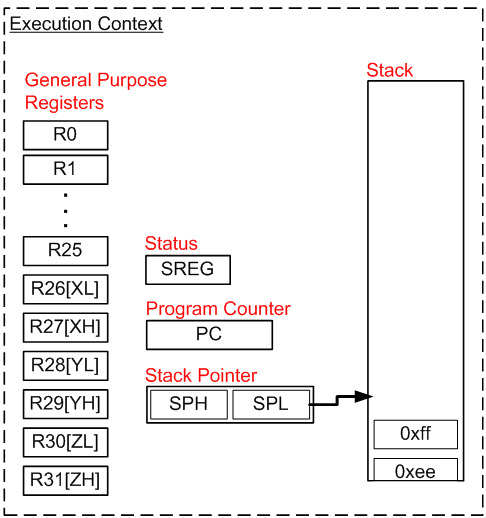
\includegraphics[scale=1]{RTOS/f5.PNG}
\end{figure}

\paragraph{Guardado del contexto}

Cada tarea de tiempo real tiene su propio espacio en la memoria de la pila así que el contexto puede guardarse simplemente haciendo "push" los registros del procesador en la pila de la tarea. \\

 \textit{portSAVE\_CONTEXT()} Está implementado como un macro para el AVR, cuyo código fuente es el siguiente
 
 \begin{verbatim}
#define portSAVE_CONTEXT()           
asm volatile (	                     
  "push  r0                    nt"  (1)
  "in    r0, __SREG__          nt"  (2)
  "cli                         nt"  (3)
  "push  r0                    nt"  (4)
  "push  r1                    nt"  (5)
  "clr   r1                    nt"  (6)
  "push  r2                    nt"  (7)
  "push  r3                    nt" 
  "push  r4                    nt" 
  "push  r5                    nt" 

    :
    :
    :

  "push  r30                   nt" 
  "push  r31                   nt" 
  "lds   r26, pxCurrentTCB     nt"  (8)
  "lds   r27, pxCurrentTCB + 1 nt"  (9)
  "in    r0, __SP_L__          nt"  (10)
  "st    x+, r0                nt"  (11)
  "in    r0, __SP_H__          nt"  (12)
  "st    x+, r0                nt"  (13)
);
 \end{verbatim}

Puntos importantes a considerar del código anterior:

\begin{itemize}
    \item El registro R0 se guarda primero
    \item El registro de estado es movido hacia R0 (2) para que pueda guardarse en la pila (4).
    \item Las interrupciones del procesador son deshabilitadas (3). Si \textit{portSAVE\_CONTEXT()} fue llamado solamente desde el contenido de una interrupción ISR, no habría necesidad de deshabilitar explícitamente las interrupciones. Mientras que si la macro se usa también por fuera de rutinas de interrupciones (cuando una tarea se suspende a sí misma) las interrupciones debes ser claramente deshabilitadas tan pronto como sea posible.
    \item El código generado por el compilador del código en C del ISR asume que el valor de R1 es cero. El valor original de R1 se guarda (5) antes de que se limpie (6).
    \item Entre (7) y (8) los reistros restantes se guardan en orden numérico.
    \item La pila de la tarea que se suspende ahora contiene una copia del contexto de ejecución de tarea. El kernel almacena el apuntador de la pila de la tarea, así el contexto puede ser recuperado cuando la tarea se reanude. El registo X se carga con la dirección hacia la cual el puntero se va a guardar. 
    \item El apuntador se guarda.
\end{itemize}

\paragraph{Restauración del contexto}

La macro \texttt{portRESTORE\_CONTEXT()} hace exactamente lo contrario a la anterior, restaura el contexto de una tarea una vez esté lista. Los registros que están almacenados en la pila de la tarea son recuperados por el kernel del SO y se almacenan de nuevo en los registros principales.

\begin{verbatim}
#define portRESTORE_CONTEXT()        
asm volatile (	
  "lds  r26, pxCurrentTCB      nt"  (1)
  "lds  r27, pxCurrentTCB + 1  nt"  (2)
  "ld   r28, x+                nt"  
  "out  __SP_L__, r28          nt"  (3)
  "ld   r29, x+                nt"  
  "out  __SP_H__, r29          nt"  (4)
  "pop  r31                    nt" 
  "pop  r30                    nt" 

    :
    :
    :

  "pop  r1                     nt" 
  "pop  r0                     nt"  (5)
  "out  __SREG__, r0           nt"  (6)
  "pop  r0                     nt"  (7)
);

\end{verbatim}

\begin{itemize}
    \item La variable \texttt{pxCurrentTCB} propia de FreeRTOS mantiene la dirección hacia donde el puntero de pila de la tarea puede recuperar. Este se carga en el registro X (1 y 2)
    \item El puntero de pila para la tarea que se va a resumir se carga al puntero de pila del AVR, primero el byte menos significativo y luego el más significativo.
    \item Los registros principales se establecen de la pila en orden inverso. 
    \item El registro de estado guardado en la pila entre lo registros R1 y R0 también se restauran.
\end{itemize}

\subsubsection{Ejemplo detallado}

En el siguiente ejemplo se muestra y se explica el cambio de un contexto de ejecución de tarea; de una tarea A de menor prioridad a una tarea B de mayor prioridad.

\paragraph{Antes de la interrupción por el tick}

Este ejemplo empieza con la tarea A ejecutándose. La tarea B había sido suspendida anteriormente por lo que su contexto ya se había guardado en su correspondiente pila.


\begin{figure}[H]
    \centering
    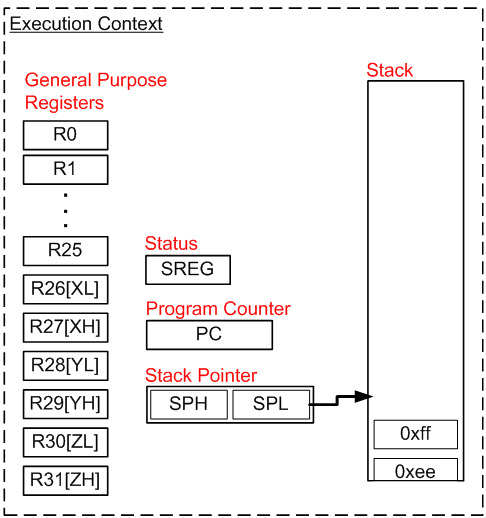
\includegraphics[scale=0.7]{RTOS/f5.png}
\end{figure}

Todo lo anterior corresponde a registros y datos que pertenecen al contexto de la tarea A.

\paragraph{La interrupción por tick ocurre}

el evento del tick de RTOS ocurre justo cuando la tarea A está a punto de ejecutar una istrucción LDI. Cuando la interrupción ocurre el MCU AVR sitúa automáticamente el contador del programa (PC) en la pila antes de dirigirse a la rutina de interrupción del tick.

\begin{figure}[H]
    \centering
    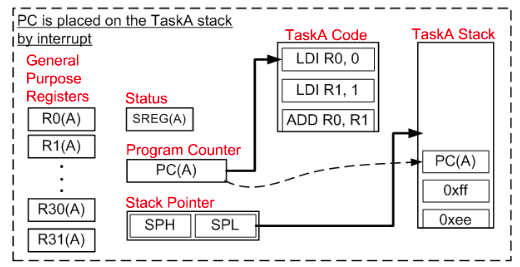
\includegraphics[scale=0.7]{RTOS/f6.PNG}
\end{figure}

\paragraph{Se ejecuta la interrupción del tick}

El código de la interrupción se puede ver a continuación.

\begin{verbatim}
/* Interrupt service routine for the RTOS tick. */
void SIG_OUTPUT_COMPARE1A( void )
{
    vPortYieldFromTick();
    asm volatile ( "reti" );
}
/*--------------------------------------------------*/

void vPortYieldFromTick( void )
{
    portSAVE_CONTEXT();

    vTaskIncrementTick();
    vTaskSwitchContext();
    portRESTORE_CONTEXT();

    asm volatile ( "ret" );
}
/*--------------------------------------------------*/
\end{verbatim}

la función \texttt{SIG\_OUTPUT\_COMPARE1A()} es del tipo 'naked', así la primera instrucción es un llamado al método \texttt{vPortYieldFromTick()} la cual es también 'naked' y el contexto de ejecución del AVR se guarda explícitamente a través del llamado a \texttt{portSAVE\_CONTEXT()}.

La función anterior guarda enteramente el contexto de ejecución en la pila de la tarea A. El puntero de esta pila apunta ahora al inicio de su propio contexto. \texttt{portSAVE\_CONTEXT} termina con guardar una copia del puntero de pila. El kernel de tiempo real ya tiene también una copia del puntero de pila de la tarea B que fue tomada en el momento en que esta fue suspendida.

\begin{figure}[H]
    \centering
    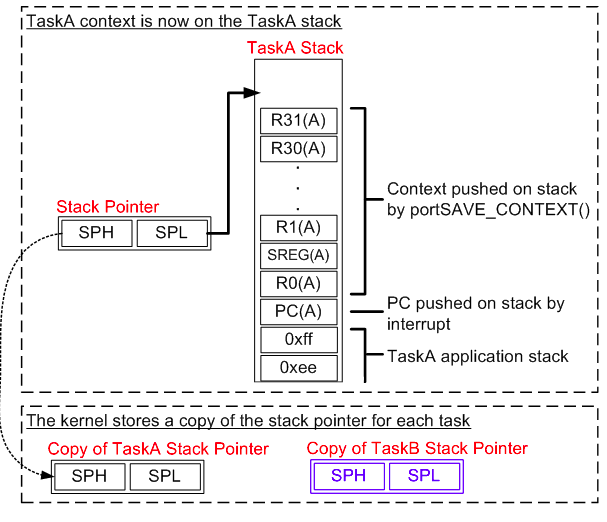
\includegraphics[scale=0.7]{RTOS/f7.PNG}
\end{figure}

\paragraph{Incremento del contador de Tick}

\texttt{vTaskIncrementTick()} se ejecuta después de que el contexto de la tarea A se guarda. Para los propósitos de este ejemplo se asume que el incremento del contador del tick ha causado que la tarea B se vuelva disponible para ser ejecutada. La tarea B tiene una prioridad mayor a la de A así que \texttt{vTaskSwitchContext()} selecciona a la tarea B para darle tiempo de ejecución al momento de que se complete la ISR.

\paragraph{Se recupera el puntero de pila de la tarea B}

\begin{figure}[H]
    \centering
    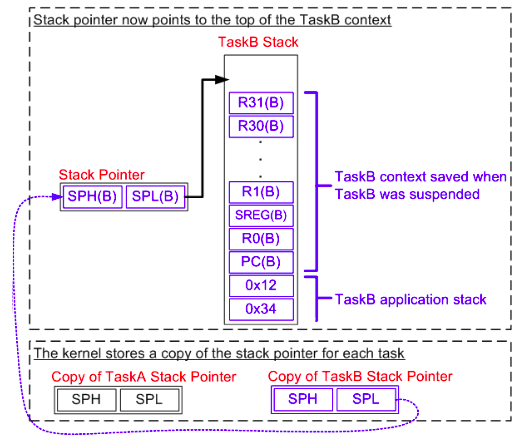
\includegraphics[scale=0.7]{RTOS/f8.PNG}
\end{figure}

Ahora la tarea B debe ser restaurada. Lo primero que hace la macro de RTOS \texttt{portRESTORE\_CONTEXT} es recuperar el puntero de pila de la tarea B de la copia que se había creado previamente a la suspensión de la tarea. El puntero de pila se carga al puntero de pila del procesador, ahora este apunta al tope del contexto de ejecución de Tarea B.

\paragraph{Restauración del contexto de B}

\texttt{portRESTORE\_CONTEXT()} se completa con la restauración del contexto de ejecución de la tarea B desde su pila hacia los registros principales correspondientes.

\begin{figure}[H]
    \centering
    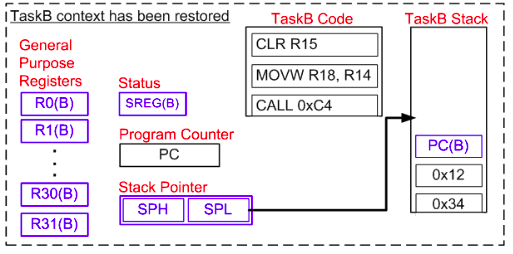
\includegraphics[scale=0.7]{RTOS/f9.PNG}
\end{figure}

Solamente el contador del programa es el que permanece en la pila de TaskB.

\paragraph{El tick de RTOS termina}

\texttt{vPortYieldFromTick()} retorna hacia \texttt{SIG\_OUTPUT\_COMPARE1A()} en la que la última instrucción es un retorno de interrupción \texttt{RETI}. Una instrucción de retorno de este tipo asume que el siguiente valor de la pila es una dirección de retorno que se puso en la pila cuando ocurrió la interrupción.

\begin{figure}[H]
    \centering
    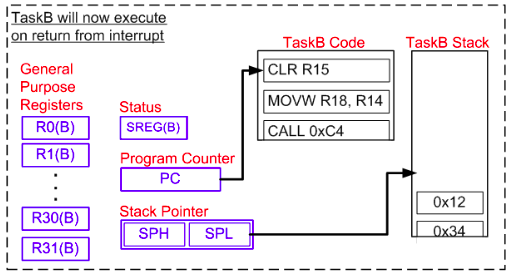
\includegraphics[scale=0.7]{RTOS/f10.PNG}
\end{figure}

Cuando la interrupción por tick empezó, el AVR automáticamente situó la dirección de retorno de la tarea A en la pila (la dirección de la siguiente instrucción a ejecutar de la tarea A). El manejador de tick de RTOS alteró el puntero de pila para que apuntara ahora a la pila de la tarea B. Entonces la dirección de retorno extraída de la pila por la instrucción RETI es ahora la dirección de instrucción de la tarea B que se iba a ejecutar inmediatamente antes de que fuera suspendida.  

\subsection{Concepto de las Tareas y co rutinas}

    \subsubsection{Introducción}
    
    Cada tarea es un pequeño programa. Tiene un puntero de entrada el cual se ejecuta en un blucle infinito normalmente. Una sola definición de una función \texttt{vTask} puede ser utilizada para crear cualquier número de tareas (cada tarea siendo una instancia separada de ejecución). \\
    
    Una aplicación puede tener varias tareas. Si el procesador que ejecuta la aplicación contiene solo un núcleo, entonces solamente se puede ejecutar una tarea al tiempo. 
    
    \paragraph{Características de una tarea}
    
    
    Una aplicación en tiempo real que utilice un RTOS puede estar estructurado como un conjunto de tareas independientes. Cada tarea se ejecuta dentro de su propio contexto sin ninguna dependencia de otras tareas en el sistema o en el planificador del sistema. Solamente una tarea dentro de la aplicación puede ser ejecutada en cualquier punto del tiempo y el planificado del sistema operativo de tiempo real es el responsable de decidir cuál es la tarea que se está ejecutando. El planificador por lo tanto puede iniciar y parar repetidamente cada tarea. Ya que una tarea no tiene conocimiento de la actividad del planificador, es la responsabilidad de este último asegurarse de que el contexto del procesamiento cuando una tarea vaya a ejecutarse sea el mismo contexto que había cuando la misma tarea dejó de ejecutarse en el pasado. Para cumplir con esto cada tarea tiene su propia pila.
    
    Cuando la pila es cambiada para dejar de ejecutar una tarea, el contexto de ejecución se guarda en esta pila.
    
    \paragraph{Características de una co-rutina}
    
    \subparagraph{Nota} Las co-rutinas fueron implementadas para el uso en dispositivos realmente pequeños, pero son usados muy raramente en la actualidad. \\
    
    Son conceptualmente muy similares a las tareas, y sus diferencias fundamentales son las siguientes
    
    \begin{enumerate}
        \item Uso de pila: Todas las corrutinas en una aplicación comparten una sola pila. Esto reduce grandemente el uso de memoria RAM del dispositivo.
        \item Planificación y prioridades: las rutinas de este tipo usan planificaciones cooperativas priorizadas con respecto a otras rutinas, pero pueden ser incluidas en aplicaciones que utilizan tareas. 
        \item La implementación de las corrutinas se proporciona a través de macros. 
    \end{enumerate}
    
    \subsubsection{Estados de una tarea}
    
    \paragraph{Ejecutando}
    
    Cuando una tarea se está ejecutando actualmente se dice que está en este estado. Está haciendo uso del procesador en ese momento. Si el procesador en el que se está ejecutando el RTOS tiene un solo núcleo entonces solo puede haber una tarea que esté en este estado.
    
    \paragraph{Lista}
    
    Las tareas en este estado son aquellas que tienen la posibilidad de ser ejecutadas, pero no se están ejecutando en ese momento porque otra tarea con una prioridad mayor es la que se está ejecutando. 
    
    \paragraph{Bloqueada}
    
    Se dice que una tarea está en este estado de bloqueo si en un tiempo está esperando por un evento sea externo o temporal. Por ejemplo si una tarea se llama \texttt{vTaskDelay()} esta estará bloqueada hasta que el periodo de delay haya expirado (evento temporal). Las tareas también se pueden bloquear para esperar una cola, semáforo, etc. Las tareas en este estado normalmente tienen un periodo de 'tiempo límite', después de este aunque el evento que sea que esté esperando no ocurra, esta tarea se desbloqueará.
    
    \paragraph{Suspendido}
    
    Así como las tareas que están en el estado de bloqueadas, aquellas que están suspendidas no pueden ser seleccionadas para entrar al estado de ejecución, la diferencia de este estado con el anterior es que no cuenta con un 'tiempo límite'. En lugar de eso las tareas solamente pueden entrar o salir de el estado suspendido cuando se les indica explícitamente en código, a través de \texttt{vTaskSuspend()} y \texttt{xTaskResume()}.
    
    
    \begin{figure}[H]
        \centering
        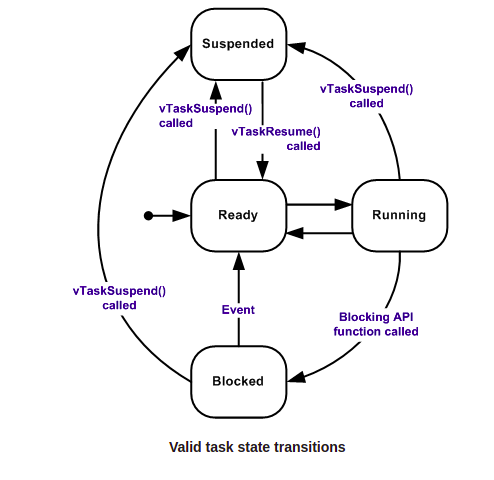
\includegraphics[scale=0.7]{RTOS/f11.PNG}
    \end{figure}
    
    
    \subsubsection{Prioridades de las tareas}
    
    A cada tarea se le asigna una prioridad que va desde 0 hasta \texttt{configMAX\_PRIORITIES} -1, donde \texttt{configMAX\_PRIORITIES} está configurado dentro de \texttt{FreeRTOSConfig.h}
    
    Si la tarjeta que se usa implementa un mecanismo de selección de tarea optimizada que utilice una instrucción del tipo "contador de ceros iniciales" y \texttt{configUSE\_PORT\_OPTIMISED\_TASK\_SELECTION} se establece en \texttt{1}, entonces \texttt{configMAX\_PRIORITIES} no puede ser mayor a 32. En todos los demás casos este puede tener cualquier valor.\\
    
    Números pequeños de prioridad denota tareas de baja prioridad. La tarea inactiva (idle task) tiene prioridad cero (\texttt{tskIDLE\_PRIORITY}). 
    
    El planificador del sistema operativo se asegura de que cualquier tarea que esté en estado Listo o Ejecutando siempre tenga su respectivo tiempo de procesamiento disponible en preferencia sobre las tareas que tengan una prioridad menor y que estén en el estado Lista. Dicho de otra forma, aquella tarea que esté en el estado Ejecución siempre será la tarea de mayor prioridad entre las que se encuentren listas o disponibles. 
    
    Pueden existir cualquier número de tareas que compartan la misma prioridad. Si el valor de \texttt{configUSE\_TIME\_SLICING } no está configurado o si su valor es igual a 1, entonces las tareas en el estado listas que tengan la misma prioridad compartirán el tiempo de procesamiento disponible mediante un esquema de planificación de turnos.
    
    \subsubsection{Planificación de las tareas}\label{plan_tar}
    
    El algoritmo de planificación es la rutina que decide cuál es la tarea que está en el estado ejecución. Solamente puede haber una tarea en este estado por cada núcleo de procesamiento. AMP (asymmetric multicore) es donde cada núcleo del procesador ejecuta su propia instancia de FreeRTOS. SMP (symmetric multicore) es donde hay una instancia de FreeRTOS que planifica las tareas a lo largo de los múltiples núcleos.
    
    \paragraph{Política por defecto de planificación para un núcleo}
    
    El sistema operativo utiliza una política de planificación de tareas con el mismo nivel de prioridad. Las palabras clave son "fixed-priority" "preemptive", "round-robin", "time-slicing".
    
    \begin{itemize}
        \item "Fixed priority" Significa que el planificador no cambia la prioridad de una tarea de forma permanente, aunque puede 'acelerar' temporalmente la prioridad de una tarea debido a herencia de prioridad.
        \item "Preemptive" Significa que el planificador siempre ejecuta la tarea de mayor prioridad que esté disponible o lista independientemente de cuándo puede volverse disponible. Por ejemplo si un ISR cambia la tarea disponible con más alta prioridad, el planificador va a detener la tarea actual de menor prioridad e inciará la de mayor.
        \item "Round-robin" significa que las tareas que tengan la misma prioridad se turnan para entrar en el estado de ejecución. 
        \item "Time sliced" significa que el planificador cambia de tareas de igual prioridad en cada interrupción de tick.
    \end{itemize}
    
    \subparagraph{Uso de planificador preventivo priorizado}
    
    Una de las consecuencias de que siempre se ejecute la tarea de mayor prioridad que esté disponible, es que una tarea de alta prioridad que nunca entra en los estados bloqueado o suspendido, va a estar permanentemente privando a las tareas de menor prioridad de tiempo de ejecución. Esta es una razón por la que normalmente siempre es mejor crear tareas que sean manejadas mediante eventos. Por ejemplo si una tarea de alta prioridad está esperando a que suceda un evento, no debería caer en un bucle por el evento gracias a que constantemente se está realizando sondeo, y tampoco en el estado de bloqueado o suspendido. En lugar de eso, la tarea debería entrar en el estado de bloqueado para esperar por ese evento. El evento puede ser enviado a la tarea a través de as primitivas de comunicación y sincronización inter tareas de FreeRTOS. Recibiendo el evento automáticamente se quita la tarea de alta prioridad del estado bloqueado. La tarea de prioridad más baja entonces se ejecutará mientras la de alta permanece en el estado bloqueado.
    
    \subparagraph{Configuración de la política de planificación RTOS}
    
    \begin{itemize}
        \item \texttt{configUSE\_PREEMPTION}: Si el valor de esta configuración se pone a cero entonces la configuración preventiva se apaga y el cambio de contextos solamente ocurrirá si la tarea en el estado ejecutando entra al estado de bloqueo o suspensión, la tarea en ejecución llama a la rutina \texttt{taskYIELD()}, o una ISR hace una solicitud manualmente para cambio de contexto.
        \item \texttt{configUSE\_TIME\_SLICING}: Si esta configuración se pone en cero, entonces los cortes (slicing) de tiempo se desactivan, de manera que el planificador no realizará cambios de tareas de igual prioridad en cada interrupción de tiempo.
    \end{itemize}
    
    \subsubsection{Implementación de una tarea}
    
    Una tarea deberá tener la siguiente estructura:
    
    \begin{verbatim}
        void vATaskFunction( void *pvParameters )
        {
            for( ;; )
            {
                -- Task application code here. --
            }
    
            /* Tasks must not attempt to return from their implementing
            function or otherwise exit.  In newer FreeRTOS port
            attempting to do so will result in an configASSERT() being
            called if it is defined.  If it is necessary for a task to
            exit then have the task call vTaskDelete( NULL ) to ensure
            its exit is clean. */
            vTaskDelete( NULL );
        }
    \end{verbatim}
    
    El tipo \texttt{TaskFunction\_t} se define como una función que retorna un void y toma un puntero void como su único parámetro. Todas las funciones que implementen una tarea deben ser de este tipo. El parámetro puede ser utilizado para pasar información de cualquier tipo hacia la tarea.
    
    Las funciones de tareas no deben tener un retorno, por lo que deberían ser siempre un bucle continuo. Sin embargo, como se indica en el apartado \ref{plan_tar}, normalmente es mejor crear tareas que sean manejadas por evento para no privar de tiempo de procesamiento a las tareas que tengan menor prioridad, a partir de la siguiente estructura:
    
    \begin{verbatim}
        void vATaskFunction( void *pvParameters )
        {
            for( ;; )
            {
                /* Psudeo code showing a task waiting for an event 
                with a block time. If the event occurs, process it.  
                If the timeout expires before the event occurs, then 
                the system may be in an error state, so handle the
                error.  Here the pseudo code "WaitForEvent()" could 
                replaced with xQueueReceive(), ulTaskNotifyTake(), 
                xEventGroupWaitBits(), or any of the other FreeRTOS 
                communication and synchronisation primitives. */
                if( WaitForEvent( EventObject, TimeOut ) == pdPASS )
                {
                    -- Handle event here. --
                }
                else
                {
                    -- Clear errors, or take actions here. --
                }
            }
    
            /* As per the first code listing above. */
            vTaskDelete( NULL );
        }
    \end{verbatim}
    
    Las tareas se crean mediante \texttt{xTaskCreate()} o \texttt{xTaskCreateStatic()} y se borran mediante \texttt{vTaskDelete()}.

\subsection{Colas y semáforos}

\subsubsection{Las colas en FreeRTOS}

Las colas son la forma principal y primaria de intercomunicación entre tareas. Pueden ser utilizadas para enviar mensajes entre tareas y entre tareas e interrupciones. En la mayoría de los casos son implementaciones de búferes FIFO. Cada nueva información a enviar se almacena al final del búfer, aunque también puede ser enviada al principio del mismo.\\

Las funciones de envío y recibimiento de datos a la cola: \texttt{xQueueSendToBack()} y \texttt{xQueueReceive()}

\paragraph{Modelo de usuario, simplicidad y flexibilidad}

El modelo de uso de las colas en FreeRTOS se administra para combinar simplicidad con flexibilidad. Los mensajes son enviados a través de las colas por copia, esto significa que los datos (los cuales pueden ser apuntadores a espacios grandes de memoria) son copiados en la cola, en lugar de la cola almacene solamente una referencia de los datos. Este es el mejor enfoque por las siguientes razones:

\begin{itemize}
    \item Mensajes pequeños que están ya de hecho contenidos en variables C (entero, estructura pequeña, etc) pueden ser directamente enviados a la cola. No hay necesidad de alojar esta información en un búfer para el mensaje y luego copiarla. De igual manera, los mensajes pueden ser leídos directamente desde la cola. Adicionalmente, esta forma permite por ejemplo soreescribir las variables que fueron enviadas a la cola, porque esa copia que se encuentra en la cola puede ser utilizada posteriormente.
    \item El uso de las colas que pasan la información mediante copia no quiere decir que no se pueda pasar información mediante referencia. Si por ejempli un mensaje es demasiadamente grande en tamaño como para ser copiado dentro de la cola, se puede definir en la cola para que esta maneje punteros hacia la información del mensaje y que estos punteros sean los que se envíen dentro de la cola.
    \item El kernel es completamente responsable de asignar la memoria utilizada como área de almacenamiento de las colas.
    \item Mensajes con tamaño variable pueden ser enviados configurando la cola de tal forma que permita tener estructuras que contengan un miembro que apunte al mensaje, y otro miembro que tenga el tamaño del mensaje.
    \item Una sola cola puede ser utilizada para recibir mensajes de distintos tipos, así como mensajes provenientes de distintas localizaciones, definiendo la cola para que contenga una estructura en la que un miembro es el tipo de mensaje y otro miembro que tenga el contenido del mensaje (o un puntero al mismo). La manera en la que se interpretan los datos depende del tipo de mensaje. 
    \item Esta implementación es naturalmente adecuada para el uso en un entorno de memoria protegida. Una tarea que está restringida a un área de memoria protegida puede pasar datos a una tarea que está restringida en otro área de memoria protegida porque invocar el RTOS llamando a la función de envío de cola aumentará el nivel de privilegio del MCU.Solo el sistema operativo (con todos los privilegios) accerde al área de almacenamiento de la cola.
    \item Un API separado o independiente está disponible para el uso dentro de las interrupciones.
\end{itemize}

\paragraph{Bloqueo en colas}

Las funciones API de colas permire que un tiempo de bloqueo sea especificado. Cuando una tarea trata de leer una cola que está vacía, la tarea entrará en el estado bloqueado (para que no consuma recursos de CPU y otras tareas puedan ser ejecutadas) hasta que alguna información o datos se haga disponible en la cola, o hasta que el tiempo de bloqueo expira.\\
Cuando una tarea trata de escribir en una cola que está llena, esta también entrará en el estado bloqueado hasta que haya espacio disponible en la cola o hasta que el tiempo de bloqueo expire.\\
Si más de una tarea se bloquea con la misma cola, entonces la tarea con mayor prioridad será la que se desbloquee primero. 

\subsubsection{Semáforos binarios}

Los semáforos binarios son utilizados tanto para exclusión mutua como para propósitos de sincronización. Los semáforos binarios y los mutex son muy similares excepto por unas pequeñas diferencias: los mutex incluyen un mecanismo de herencia prioritaria, mientras que los semáforos binarios no. Esto hace que los semáforos binarios sean el mejor recurso para implementar sincronización entre tareas o entre tarea e interrupción, y que los mutex sean la mejor opción para implementar exclusiones mutuas simples. \\

Las funciones de semáforo permiten que se especifique un tiempo de bloqueo. Dicho tiempo indica el número máximo de ticks (el tiempo) que una tarea deberá entrar en el estado de bloqueo cuando al tratar de 'tomar' un semáforo, este no esté inmediatamente disponible. Si más de una tarea se bloquea en el mismo semáforo, la tarea de mayor prioridad será la primera en ejecutarse cuando el semáforo esté disponible. \\

Se puede pensar en un semáforo binario como una cola que solamente puede tener un objeto almacenado. De esta forma la cola podrá estar solamente vacía o llena. A las tareas e interrupciones que usen la cola no les importará qué tiene la cola almacenada, solamente necesitan saber si esta está llena o vacía. \\

Considere el caso en que una tarea es usada para servir un periférico. Si se hace consulta repetitia (polling) al periférico esto gastaría innecesariamente recursos y evita que otras tareas puedan ser ejecutadas. Es preferible que la tarea permanezca más de su tiempo en el estado bloqueado (permitiendo a otras tareas ejecutarse) y solamente se ejecutará cuando verdaderamente haya algo que se deba hacer. Esto se logra mediante la implementación de un semáforo binario haciendo que la tarea se bloquee mientras trata de tomar el semáforo. Una rutina de interrupción es escrita para el periférico la cual activa el semáforo cuando el periférico necesita un servicio. la tarea siempre 'toma' el semáforo (el cual se puede interpretar como una lectura de la cola dejándola vacía), pero no puede escribirla. De este mismo modo la interrupción puede solamente escribir en la cola mas no leer de ella. \\

la prioridad de las tareas puede ser utilizada para asegurar que los periféricos sean servidos de manera oportuna.

\subsubsection{Semáforos contadores}

Así como los semáforos binarios pueden ser imaginados como una cola de un solo elemento, los semáforos contadores pueden ser imaginados como colas cuyo tamaño son mayores a uno. Nuevamente, los usuarios del semáforo no tienen interés de los datos que están almacenados en la cola, sino solo les interesa saber si está o no está vacía.\\

Los semáforos contadores son típicamente utilizados por las siguientes razones: \\

\begin{enumerate}
    \item Conteo de eventos: en este escenario de uso un manejador de tarea tomará un semáforo cada vez que procese un evento (decrementando el valor del semáforo). El valor del contador es la diferencia entre el número de eventos que han ocurrido, y el número que han sido procesados. En este caso es deseable que el valor del semáforo sea de cero cuando este es creado.
    \item administración de recursos: En este escenario el valor del contador indica el número de recursos disponible. Para obtener el control de un recurso, una tarea debe obtener primero un semáforo (decrementando el valor de su contador). Cuando el contador se hace cero, significa que ya no hay más recursos disponibles. Cuando la tarea termina de usar el recurso, se lo 'entrega' de nuevo al semáforo, aumentando nuevamente el valor del contador. En este caso es deseable que el valor del semáforo sea del máximo en el momento en el que es creado.
\end{enumerate}

\subsubsection{Mutex}

Los mutex son muy similares a los semáforos binarios que incluyen un mecanismo de herencia de prioridad. Mientras que los semáforos binarios son la mejor opción para implementar sincronización (entre tareas, o tarea-interrupción) los mutex son la mejor opción para implementar exclusiones mutuas sencillas. Cuando se usa para este propósito el mutex actúa como una 'ficha' para guardar un recurso. Cuando una tarea desea acceder al recurso primero debe obtener o 'tomar' la ficha. Cuando ha terminado de usar ese recurso, 'deja' o 'devuelve' la ficha de nuevo, con ello concede la oportunidad a otras tareas de obtener ese recurso.\\

Los mutex utilizan las mismas aplicaciones e API de los semáforos, así que también permite especificar un tiempo de bloqueo. Este tiempo indica el número máximo de ticks en que la tarea debería entrar al estado bloqueado cuando trata de 'pedir la ficha' del mutex si este no está disponible en ese momento. La herencia de prioridad significa que si una tarea de alta prioridad se bloquea mientras está esperando el mutex que está actualmente en manos de una tarea de menor prioridad, entonces la prioridad de la tarea es elevada temporalmente a aquella que está esperando la 'ficha'. Este mecanismo está diseñado para asegurar que la tarea de alta prioridad se mantenga en el estado bloqueado el menor tiempo posible.\\

\subsubsection{Mutex recursivos}

Un mutex utilizado de manera recursiva puede ser 'tomado' de manera repetida por el propietario. El mutex no se hace disponible de nuevo hasta que el propietario llama a la función \texttt{xSemaphoreGiveRecursive()} por cada solicitud de \texttt{xSemaphoreTakeRecursive()} satisfactoria. Por ejemplo, si una tarea 'toma' satisfactoriamente 5 veces entonces el mutex no estará disponible para ninguna otra tarea hasta que la tarea 'devuelva' ese mutex exactamente las 5 veces.\\

Este tipo de semáforo usa un mecanismo de herencia de prioridad, por lo que una tarea que 'toma' el semáforo \textbf{siempre tiene} que devolver el semáforo una vez no lo requiera más. Los semáforos tipo mutex no pueden ser utilzados desde el interior de una rutina de servicio de interrupción.\\

Los mutex no deberían ser usados en las interrupciones porque:

\begin{itemize}
    \item Incluyen un mecanismo de herencia de prioridad lo cual solamente tiene sentido si el mutex se toma o se recibe desde una tarea.
    \item Una interrupción no puede bloquearse para esperar un recurso.
\end{itemize}

\subsection{Notificaciones directas hacia tareas}

\subsubsection{Introducción}

Cada tarea de RTOS tiene un arreglo de notificaciones de tarea. Cada notificación de tarea tiene un estado que puede ser 'pendiente' o 'no pendiente' y un valor de notificación de 32 bits. la constante \texttt{configTASK\_NOTIFICATION\_ARRAY\_ENTRIES} configura el número de índices en el arreglo de notificaciones.\\

Una \textit{notificación directa a tarea} es un evento enviado directamente a la tarea, en lugar de enviarla indirectamente mediante un objeto intermediario como por ejemplo una cola, un grupo de eventos o un semáforo. Al enviar una notificación directa a una tarea el estado de la notificación de la tarea pasa a ser 'pendiente'. Así como una tarea se puede bloquear en un objeto intermediario como un semáforo para esperar a que el semáforo esté disponible, también puede bloquearse en una notificación de tarea para esperar a que el estado de dicha notificación se vuelva pendiente.\\

Con el envío de notificaciones directas hacia tareas, opcionalmente se puede actualizar el valor de la notificación objetivo de las siguientes maneras:

\begin{itemize}
    \item Sobreescribir el valor sin importar si la tarea ya ha leído el valor que se va a sobreescribir o no.
    \item Sobreescribir el alor, pero solamente si la tarea ya leyó el valor que se va a asobreescribir.
    \item Cambiar uno o mas bits en el valor.
    \item Incrementar el valor en 1.
\end{itemize}

Al llamar \texttt{xTaskNotifyWait()/xTaskNotifyWaitIndexed()} para leer el valor de una notificación, borra el estado de esa notificación a 'no pendiente'. El estado de la notificación también puede cambiarse a 'no pendiente' explícitamente mediante \texttt{xTaskNotifyStateClear()/xTaskNotifyStateClearIndexed()}.

Cada notificación dentro del arreglo opera de forma independiente - una tarea solo puede bloquearse en una notificación dentro del arreglo al tiempo y no podrá ser desbloqueada por una notificación enviada a otro índice del arreglo.\\

Estas notificaciones están por defecto habilitadas y se pueden excluir del programa configurando \texttt{ configUSE\_TASK\_NOTIFICATIONS } a cero.

\subsubsection{Restricciones y beneficios}

La flexibilidad de las notificaciones permiten que puedan ser usadas cuando, de lo contrario, habría sido necesario crear una cola separada, un semáforo binario, de conteo o un grupo de eventos. El uso de las notificaciones directas es más rápido (45\%) más rápido. Por supuesto también existen agunas limitaciones:

\begin{enumerate}
    \item Las notificaciones solamente pueden ser utilizadas cuando solamente hay una tarea que puede ser el recipiente del evento. Esta condición es cumplida en la mayoría de casos.
    \item Solamente en los casos en los que se usan notificaciones en lugar de colas: mientras recibir una tarea puede esperar por la notificación en el estado bloqueado.
\end{enumerate}

\subsubsection{Casos de uso}

Las notificaciones son enviadas con las funciones \texttt{ xTaskNotifyIndexed()} y \texttt{xTaskNotifyGiveIndexed()} y permanecen pendientes hasta el respectivo llamado de las funciones \texttt{xTaskNotifyWaitIndexed()} o \texttt{ulTaskNotifyTakeIndexed()}. Estas funciones tienen su equivalente sin el prefijo \texttt{Indexed} y son equivalentes cuando el índice es cero. 

\subsubsection{Como semáforo binario}

Desbloquear una tarea mediante una notificación directa es un 45\% más rápido y utiliza menos RAM que hacerlo mediante un semáforo binario. \\

Cuando se usa una notificación en vez del semáforo, el valor de la notificación de la tarea que recibe es el que se usa en vez del valor del contador binario del semáforo, y la función \texttt{ ulTaskNotifyTake()} (o \texttt{ulTaskNotifyTakeIndexed()}) es la que se implementa en vez de \texttt{xSemaphoreTake()}. El parámetro \texttt{xClearOnExit} de la función \texttt{ulTaskNotifyTake()} se configura a \texttt{pdTRUE} y el valor del contador se retorna a cero cada vez que la notificación es tomada. Lo cual emula el comportamiento del semáforo. Del mismo modo se usan las funciones \texttt{xTaskNotifyGive()} (o\texttt{xTaskNotifyGiveIndexed()}) o \texttt{vTaskNotifyGiveFromISR()} y su correspondiente indexada \texttt{vTaskNotifyGiveIndexedFromISR()} para reemplazar las de semáforo \texttt{xSemaphoreGive()} y \texttt{xSemaphoreGiveFromISR()}.

\begin{verbatim}
    /* This is an example of a transmit function in a generic
peripheral driver.  An RTOS task calls the transmit function,
then waits in the Blocked state (so not using an CPU time)
until it is notified that the transmission is complete.  The
transmission is performed by a DMA, and the DMA end interrupt
is used to notify the task. */

/* Stores the handle of the task that will be notified when the
transmission is complete. */
static TaskHandle_t xTaskToNotify = NULL;

/* The index within the target task's array of task notifications
to use. */
const UBaseType_t xArrayIndex = 1;

/* The peripheral driver's transmit function. */
void StartTransmission( uint8_t *pcData, size_t xDataLength )
{
    /* At this point xTaskToNotify should be NULL as no transmission
    is in progress.  A mutex can be used to guard access to the
    peripheral if necessary. */
    configASSERT( xTaskToNotify == NULL );

    /* Store the handle of the calling task. */
    xTaskToNotify = xTaskGetCurrentTaskHandle();

    /* Start the transmission - an interrupt is generated when the
    transmission is complete. */
    vStartTransmit( pcData, xDatalength );
}
/*-----------------------------------------------------------*/

/* The transmit end interrupt. */
void vTransmitEndISR( void )
{
BaseType_t xHigherPriorityTaskWoken = pdFALSE;

    /* At this point xTaskToNotify should not be NULL as
    a transmission was in progress. */
    configASSERT( xTaskToNotify != NULL );

    /* Notify the task that the transmission is complete. */
    vTaskNotifyGiveIndexedFromISR( xTaskToNotify,
                                   xArrayIndex,
                                   &xHigherPriorityTaskWoken );

    /* There are no transmissions in progress, so no tasks
    to notify. */
    xTaskToNotify = NULL;

    /* If xHigherPriorityTaskWoken is now set to pdTRUE then a
    context switch should be performed to ensure the interrupt
    returns directly to the highest priority task.  The macro used
    for this purpose is dependent on the port in use and may be
    called portEND_SWITCHING_ISR(). */
    portYIELD_FROM_ISR( xHigherPriorityTaskWoken );
}
/*-----------------------------------------------------------*/

/* The task that initiates the transmission, then enters the
Blocked state (so not consuming any CPU time) to wait for it
to complete. */
void vAFunctionCalledFromATask( uint8_t ucDataToTransmit,
                                size_t xDataLength )
{
uint32_t ulNotificationValue;
const TickType_t xMaxBlockTime = pdMS_TO_TICKS( 200 );

    /* Start the transmission by calling the function shown above. */
    StartTransmission( ucDataToTransmit, xDataLength );

    /* Wait to be notified that the transmission is complete.  Note
    the first parameter is pdTRUE, which has the effect of clearing
    the task's notification value back to 0, making the notification
    value act like a binary (rather than a counting) semaphore.  */
    ulNotificationValue = ulTaskNotifyTakeIndexed( xArrayIndex,
                                                   pdTRUE,
                                                   xMaxBlockTime );

    if( ulNotificationValue == 1 )
    {
        /* The transmission ended as expected. */
    }
    else
    {
        /* The call to ulTaskNotifyTake() timed out. */
    }
}

\end{verbatim}












\section{RT-Thread}

https://www.rt-thread.io/

\section{PyRTOS}

https://github.com/Rybec/pyRTOS

https://pythonrepo.com/repo/Rybec-pyRTOS-python-miscellaneous
https://opensource.com/article/20/7/python-rt-thread



% \begin{figure}[H]
%     \centering
%     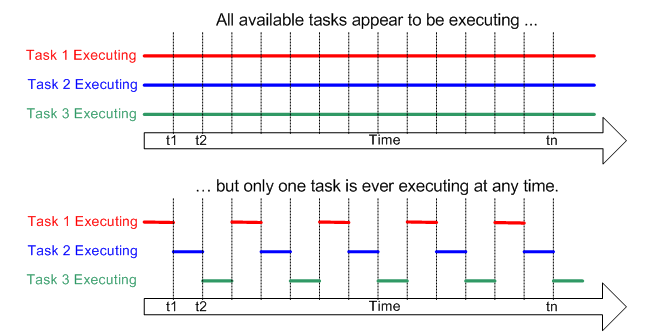
\includegraphics[scale=0.7]{RTOS/f1.PNG}
% \end{figure}
% \chapter{Redes de telecomunicaciones}

\subsection{DNS}

Significa sistemas de nombres de dominio, y su caracteristicas principal es convertir el nombre de cualquier página en su dirección IP correspondiente. 

\section{Modelos}

\subsection{Modelo TCP/IP}

Está dividido en capas, es más fácil desarrollar y diagnosticar.

Importante el tema de la estandarización, con ello todos los dispositivos hablan el mismo idioma y se pueden comunica entre ellos. 

en los años setenta, se implantó en la red ARPANET fue desarrollada por encargo para la agencia ded departamento de de defensa de los Estados Unidos.

Diseñan 4 niveles, cada cual con funciones específicas. 

Según el tipo de comunicación, puede necesitarse diferentes velocidades y formas de la transmisión de los datos. 


\subsection{modelo OSI}

En los 80's ISO realiza una estandarización de TCP/IP. Significa Modelo de interconexión de sistemas abiertos. Los niveles ahora son 7. 
\subsubsection{Niveles distintos}

\begin{enumerate}
    \item Físico: cables, hardware, tensiones.
    \item Enlace de datos: prepara la información que llega de niveles superiores. Acceso a los medios
    \item Red: Direccionamiento y elección de mejor ruta
    \item Transporte: Define cómo se trata la aplicación, según el tipo de información. 
    \item Sesión: Comunicación entre Hosts
    \item Presentación: Representación de los datos
    \item Aplicación: Procesos de red a aplicaciones
\end{enumerate}

IP y número MAC son únicas siempre, no pueden haber repetidas, es como una forma de identificación.

MAC es dirección física, IP es dirección lógica.


\section{Principios de redes y topologías}

\subsection{Encapsulamiento de los datos}

En el envío de la información, los datos viajan a través de las capas y se va cambiando su formato o forma de representación. 

\begin{enumerate}
    \item Crear los datos. Un mensaje de correo electrónico se convierte en datos de caracteres, etc.
    \item Empaquetar los datos para envío de extremo a extremo. Estos datos se empaquetan para recorrer la internetwork. Al utilizar segmentos, la función de transporte asegura que los hosts del mensaje en ambos extremos del sistema de correo electrónico se puedan comunicar de forma confiable.
    \item Agregar al encabezado la direción de red. Los datos se colocan en un paquete en cuya cabecera o encabezado se colocan las direcciones lógicas de origen y de destino. Estas direcciones facilitan el envío de los paquetes a través de de la red por una ruta seleccionada.
    \item Agregar al encabezado de enlace de datos la dirección local. Cada dispositivo de la red debe poner el paquete dentro de una trama. La trama le permite conectarse al próximo dispositivo de red conectado directamente al enlace. 
    \item Realizar la conversión a bits para la transmisión. La trama se convierte en sus equivalentes códigos binarios y esta es la información o señal que se transmite por el cable o por el medio que corresponda.
\end{enumerate}

Cada capa del modelo del equipo de origen se comunica con su capa equivalente en el equipo de destino. Esto es la comunicación par a par.

\subsection{Sistemas de clableado estructurado}

Dentro de un edificio el cableado se divide en tramos o secciones muy bien definidas. Cada sección tiene sus correspondientes equipos  sus funciones específicas.

\subsubsection{Punto de demarcación}

Llamado en inglés como demarc; es el punto que divide el cableado externo del proveedor y el cableado interno perteneciente al cliente. Representa el límite de la responsabilidad entre estos dos actores. El estándar TIA/EIA-569-A da las especificaciones de los requisitos para el espacio del demarc.

\subsubsection{Salas de equipamiento}

El cableado que sale del punto de demarcación va hacia la instalación de entrada que se encuentra en la sala de equipamiento. Esta sala es el centro de red de voz y datos. La sala de equipamiento es esencialmente una gran sala de telecomunicaciones que puede albergar el marco de distribución, servidores de red, routers, switches, PBX telefónico, protección secundaria de voltaje, receptores satelitales, moduladores y equipos de Internet de alta velocidad, entre otros.

Son regidos por los estándares TIA/EIA-569-A.

\section{Capa 3: RED}


\subsection{IPv4}



Las direcciones de clase A solo incluyen direcciones desde 1 hasta 126.

1.x.x.x hasta 126.x.x.x

El rango de 127.x.x.x se reservan para las direcciones IP de loopback o monitoreos.

Las direcciones de clase B incluyen las direcciones desde 128 hasta 191.

desde 128.0.x.x hasta 191.255.x.x

Tiene 16384 direcciones de red posibles ($2^14$), y 65534 direcciones de host($2^16-2$).

Las direcciones de clase C solo incluyen direcciones desde 192 hasta 223. 

192.0.0.x hasta 223.255.255.x

Son 2097152 ($2^21$) direcciones de red y 254 direcciones de host. \\

Hay diferencias entre IPs públicas y privadas, las primeras están en internet y las demás son reservadas para LAN's.\\

Rangos para direcciones privadas:

\begin{itemize}
    \item Clase A: 10.0.0.0 hasta 10.255.255.255
    \item Clase B: 172.16.0.0 hasta 172.31.255.255
    \item Clase C: 192.168.0.0 hasta 192.168.255.255
\end{itemize}

 La IP de RED es la que tiene todos sus bits de hosts en \textbf{cero}. Ej: 10.0.0.0/8
 
 La IP de BROADCAST es en la que todos sus bits de host en \textbf{uno}. Ej: 10.255.255.255/8
 
 Las IP's válidas son todas las demás y son las que se pueden asignar a los dispositivos. 


\subsection{IPv6}

Tienen una longitud de 128 bits, y se escriben en formato \textbf{hexadecimal}.

están compuestos por 32 dígitos hexadecimales.\\

\texttt{2001:0DB8:AC10:FE01:0000:0000:0000:0000}

En IPv6 se implementa el uso del slash para identificar la sección perteneciente para redes y para host.

En este caso el prefijo es el nombre adecuado para la sección de red, y la interfaz para sección de host.

\texttt{2001:DB8:A::/64}

Aquí ya no hay una dirección de broadcast, solo la de red y las válidas.

\subsubsection{Conversion IPv4 a IPv6}

Sea \texttt{192.168.20.112}

su binario es\\

\texttt{11000000.10101000.00010100.01110000}

Se agrupan en 4\\

\texttt{1100 0000 1010 1000:0001 0100 0111 0000}

Se convierte a Hexadecimal\\

\texttt{C0A8:1470}

Y se expande a IPv6 de la siguiente manera

\texttt{::FFFF:C0A8:1470}

Siempre se ponen 5 hextetos de ceros seguidos de cuatro \texttt{F}.\\

\subsubsection{Unicast}
Es un broadcast controlado. Se usa para identificar una interface de nodo. Un paquete enviado a una dirección unicast es entregado a la interface por esa dirección. \\

Las unicast globales constan de tres partes:

\begin{enumerate}
    \item Prefijo global, tienen el número \texttt{001} binario en el inicio: \texttt{2000} hasta \texttt{3FFF}. Son para redes públicas o globales.
    \item las de enlace local el primer hexteto da en el rango \texttt{FE80::/10} y permite conectividad local inmediata.
\end{enumerate}




\subsubsection{Multicast}

Se usa para identificar a un grupo de interfaces IPv6.


\subsection{Capa de transporte}

Define la manera en que son enviados los paquetes a partir del tipo de paquete (voz, stream, mail, etc). Es como la interfaz entre la aplicación y la red. 

Mantiene la comunicación de aplicaciones. Prepara y separa el flujo de datos para enviarse a través de los medios en partes manejables.
Realiza la identificación de aplicaciones. Los protocolos TCP y UDP denominan a este identificador un número de puerto.\\

En algunos casos \textbf{todos los datos} deben recibirse sin importar si se tienen retrasos: un correo electrónico.\\

En otros casos, una aplicación puede tolerar cierta pérdida de datos durante la transmisión de red, pero necesita velocidad de transmisión.\\

\subsubsection{UDP}

Protocolo de datagrama de usuario, sistema de nombres de dominio (DNS) Streaming video Voz sobre IP (VOIP).

DNS guarda y relaciona las direcciones IP con los nombres de dominio. 

La navegación se hace en http y estos paquetes se hacen en TCP. Sin embargo la consulta al DNS se hace por UDP. Se necesita rapidez en la consulta del nombre del dominio.

\subsubsection{TCP}

Orientado a la conexión, más recibo, bandera de retransmisión, navegación, correo, pérdida de información es más crítico. Por aquí se hace la encriptación de paquetes. 

\subsection{Capa de aplicación}

Servicios TCO/IP estándar:

\begin{itemize}
    \item FTP: El protocolo de transferencia de archivos
    \item TFTP: El protocolo de transferencia de archivos trivial
    \item Telnet: Proporciona una interfaz de usuario a través de la cual se pueden comunicar dos hosts caracter por caracter o línea por línea.
    \item SSH (Secure Shell) Hace posible que un cliente inicie una sesión interactiva en una máquina remota para envia comandos o ficheros a través de un canal seguro.  
    \item DNS Sistema de nombre de dominio que proporciona nombres al host
    \item LDAP Servicio de directorios, que proporciona las mismas funciones que un servicio de nombres con funcionalidades adicionales.
    \item Administración de la red. El protocolo simple de admin de red (SNMP) permite vr la distribución de la red y el estado de los equipos clave. SNMP también permite obtener estadísticas de red complejas del software basado en una GUI.
\end{itemize}






\section{Comandos de configuración}

La exclusión es muy importante en DHCP. Algunas IP's se deben asignar manualmente, como la de los servidores. 


Se define el IP de red que se va a utilizar para cada red.
 
 
En la configuración del terminal para los routers, se usan los siguientes comandoss

\texttt{enable} \\
\texttt{configure terminal} \\
\texttt{interface gigabitEthernet 6/0} esto es para entrar en la interfaz del puerto gigaEthernet 6/0 que es el que está conectado al switch. \\
\texttt{no shutdown} para activarlo. \\
\texttt{ip address xxx.xxx.xxx.xxx xxx.xxx.xxx.xxx} \\

se hace ctrl+z para volver al router \\ 

\texttt{write} para guardar la configuración. \\

Con esto se configuran las ip's de manera manual, para hacer dhcp: \\

\texttt{configure terminal} \\
\texttt{ip dhcp pool nombre} \\
\texttt{network (IP de red y mascara)} \\
\texttt{default-router (IP)} \\
\texttt{dns-server (IP)} \\
\texttt{exit} para salir a config, porque desde ahí se hace la exclusion. \\
\texttt{ip dhcp excluded-address (IP's inicio y fin)} \\
    
volver a guardar configuración \\


\texttt{show running config} muestra toda la configuracion hecha.\\


Para hacer enrutamiento estático.\\

\texttt{ip route IP\_de\_red\_destino Ip\_entrada} \\

Importante hacer la configuración para cada dirección (ida y vuelta)



\texttt{}



\subsection{VLAN}

Una LAN virtual sirve para hacer de una red física, varias redes. \\

Se queda en los switches.

Redes lógicas. Pueden ser con una red física. UN atque solo podría afectar una lan virtual y no a toda la lan.

Es necesario definir cuáles puertos reciben terminales, y cuáles van a estar conectados a otros witches o routers. Los primeros son puertos de acceso. Los segundos son puertos troncales. Todas las vlan deben estar configuradas entre sí. \\

switch(config) interface range fa0/1-4 -> definimos primero el rango. \\

switch(config-if-range) switchport mode trunk -> modo troncal \\

switch(config) vlan xx\\
switch(config-vlan) name yyyy \\


ejemplo: vlan 10 -> IP 192.168.10.0/24
ejemplo: vlan 20 -> IP 192.168.2    0.0/24
ejemplo: vlan 30 -> IP 192.168.30.0/24
 
La VLAN número 1 o nativa no se debe configurar, no se debe tocar.

switch(config-if-range) switchport mode acces -> modo acceso\\

switch(config-if-range) switchport acces vlan 10 -> asignación de vlan a los puertos.\\

sh vlan brief -> para ver un resume de los puertos.



\section{Vlans}

Generación de varias LAN's virtuales a partir de una física.\\

Es un concepto que se queda en los switches. Es una configuración de \textbf{nivel 2}. Son útiles para reducir el tamaño del dominio del broadcast. Ayuda también en la administración de la red, separando segmentos lógicos de una red de área local. En la parte de la seguridad, ayuda a sectorizar los fallos en la seguridad a la VLAN infectada.\\

Dos conceptos importantes: Puertos que reciben \textbf{terminales} \textbf{(acceso)} y cuáles estarán conectados a otros switches \textbf{(troncales)}.

Un puerto de acceso solo puede transportar información de una sola vlan, mientras que los puertos troncales pueden transportar tráfico de múltiples vlans. Las vlans deben estar configuradas en todo el camino, en cada switch por el que pasan.\\

Para crearlas se usan los siguientes comandos:\\

\begin{verbatim}
    switch(config)#vlan xx
    switch(config-vlan)#name YYYY
\end{verbatim}

Se asignan los nombres de las vlans coherentemente:

Gestión: vlan 10 -> IP 192.168.10.0/24
Profesores: vlan 20 -> IP 192.168.20.0/24
Alumnos: vlan 30 -> IP 192.168.30.0/24 \\\


Como los switches tienen tantos puertos, se pueden configurar rangos de los puertos. \\

\begin{verbatim}
    switch(config)#interface range fa0/1-4
    switch(config-if-range)#switchport mode trunk
    switch(config-if-range)#switchport mode access
    switch(config-if-range)#switchport acces vlan 10
\end{verbatim}

Hay una vlan nativa en cada switch, esta no se debe configurar y no se debe tocar. Generalmente una sectorización de nivel 2 con vlans viene acompañada de una sectorización de nivel 3 con diferentes direcciones IP de red. Para eso se utiliza un protocolo que es el 802.1Q\\

Este anterior protocolo permite a múltiples redes compartir de forma transparente el mismo medio físico, sin problemas de interferencia.\\

En el router se crean varias sub interfaces para cada vlan.

\begin{verbatim}
    router#configure term
    router(config)# interface fastEthernet 0/0
    router(config-if)#no shutdown
    router(config-if)# interface fastEthernet 0/0.10
    router(config-subif)# encapsulation dot1Q 10
    router(config-subif)#ip address XXXXXXX XXXXXXX
\end{verbatim}


Lo anterior es para la \textbf{vlan 10}.
% \chapter{Mejoramiento planta de asfalto}

El sistema alterno de control de la planta de asfalto CMI se compone de cuatro programas de los cuales tres son dispositivos esclavos y el restante es maestro.

\section{Esclavo 1: Estado Motores}

Se declaran variables de tipo \texttt{char} con las entradas de cada uno de los motores y máquinas de la planta, se inicializan con el valor de caracter \texttt{"0"}. Adicionalmente, se declaran tres valores \texttt{double} para temperaturas de casa de bolsas, mezcla y presión de la casa de bolsas. Un entero llamado \texttt{BytesEnBuffer} iniciado en cero, entero llamado  \texttt{lectura}, carácter llamado \texttt{lectura2}, carácter llamado \texttt{Lectura}, entero \texttt{posDatoLeido = 0}, \textbf{pos = 0}. Cadenas de tamaño 100 llamados \texttt{DatoLeido}, \texttt{Dato\_a\_enviar}, \texttt{DatoAnalogo\_a\_enviar}, \texttt{Dato\_de\_Maestro}, \texttt{Dato\_de\_Maestro\_para\_Esclavo2}  enteros llamados \texttt{a} y \texttt{b}. Finalmente se declaran los números de los pines para los estados de cada uno de los motores

\subsection{configuración \texttt{setup}}


Se configuran lo pines de entrada \texttt{Estadoxxx} como entradas con \texttt{pullup}. Se inicializa el Ethernet y el servidor con UDP. Ademas se inicia comunicación serial.

\subsection{\texttt{void loop}}

Lo que se hace en el blucle principal es ejecutar dos subrutirnas: \texttt{LecturaPuertos()} y \texttt{Envio\_a\_Maestro()}. Finalmente tras un delay de 100ms, se ejecuta una rutina llamada \texttt{Solicitud\_servidor}.


\subsection{\texttt{LecturaPuertos()}}

Realiza lectura de las entradas digitales, si estas se activan, entonces cambia cada una de las variables \texttt{xxxEstado} a \texttt{"1"}. En caso diferente, \texttt{"0"}. 

\subsection{\texttt{Envio\_a\_Maestro()}}

En esta rutina el programa asigna a cada uno de los índices de \texttt{Dat0\_a\_enviar} los estados leídos de las entradas digitales. Y finalmente ejecuta el envío por UDP a maestro. Esta rutina configura la ruta IP y el puerto del maestro para enviar el dato a enviar por este medio.



\subsection{\texttt{Solicitud\_servidor}} 

Esta rutina activa el puerto ethernet, revisando si hay un servidor disponible, una vez encuentra uno, escribe por este medio también los datos a enviar para poder ser visualizados y monitoreados por internet.

\section{Esclavo 2: Prender motores}

Se realizan las mismas declaraciones de variables del tipo caracter para los \texttt{xxxEntrada="0"}, del mismo modo para los \texttt{Solicitudxxx='0'}. 

\subsection{setup}

Los pines de salida se llaman \texttt{Salidaxxx}, se inician configuraciones de ethernet y UDP. Se ejecuta rutina \texttt{apagartodos()}

\subsection{void loop}

\begin{verbatim}
     EscrituraSalidas();    
     Modificar_motores();
     delay (10);                              
     leer_paquetes();
     Solicitud_servidor(); 
\end{verbatim}


\subsection{\texttt{leer\_paquetes()}}

Configura el UDP para recibir un paquete en la variable \texttt{packetBuffer} y luego asigna esta variable a \texttt{Datoleido}.

\subsection{\texttt{Modificar\_motores()}}

Asigna a las variables \texttt{Solicitudxxx} los valores leídos por \texttt{DatoLeido}. 

\subsection{\texttt{apagartodos()}}

Pone en estado alto todas las salidas digitales.

\subsection{EscriturasSalidas()}

Pone en valor bajo a cada salida dependiendo del valor enviado por \texttt{Solicitudxxx}, si este está en "1".

\section{Esclavo 3: Análogas y otros motores}

Se declaran variables iniciales del tipo \texttt{double} para los siguientes datos:
\begin{itemize}
    \item PresionCasadeBolsas
    \item TemperaturaCasadeBolsas
    \item TemperaturadeMezcla
    \item TemperaturadeAsfalto
    \item TemperaturaExaustDrum
    \item PosicionDamperBH
    \item PosicionValvulaCombustible
    \item PosicionDamperBHSolicitado
    \item PosicionDamperQuemadorSolicitado
    
\end{itemize}

También cadenas de caracteres para los mismos.
% \chapter{Intro to computational thinking and data science}

\section{Introducción y modelos de optimización}

Existen tres tipos de modelos: Modelos de optimización, modelos estadísticos y modelos de simulación.

Si se piensa en una función cuyo objetivo sea de maximizar  minimizar, es importante tener en cuenta las restricciones o reglas que dicha función debería seguir. Estas restricciones eliminan algunas de las soluciones, por simplemente no cumplir con los requerimientos.

Lo anterior puede ser considerado como la definición de un modelo de optimización

Pensar en el problema de la maleta; un ladrón debe encontrar la manera de robar las cosas con mayor valor de una casa y que todas quepan dentro de la maleta.

\begin{itemize}
    \item Hay un peso máximo de cosas
    \item Se quiere llevar más cosas de las que se pueden llevar
    \item Decisión de escoger cuáles son las cosas que hay que llevar y cuáles hay que dejar de lado
\end{itemize}

Se piensa en cada objeto como un par; valor y peso.
La maleta puede acomodar objetos con un peso total que no exceda a $w$. Sea también un vecto $L$ con tamaño $n$, que representa el conjunto de objetos disponibles. Cada elemento del vector es un objeto. 
Sea un vector $v$ que se usa para indicar cuándo se toma un objeto o no. si $V[i] = 1$, el objeto $L[i]$ se toma, si es cero, no se toma.

Matemáticamente se puede resumir el problema de optimización de la siguiente forma: encontrar un $V$ que maximice

\begin{equation}
    \sum_{i=0}^{n-1} V[i] * L[i].value
\end{equation}

sujeto a la restricción


\begin{equation}
    \sum_{i=0}^{n-1} V[i] * L[i].weight \leq w
\end{equation}


¿Cuál algoritmo puede usarse para resolver este problema de optimización?
No existe un algoritmo que no sea exponencial que pueda resolverlo; de hecho muchos problemas de optimización son inherentemente exponenciales. Así que aunque no existen soluciones exactas o perfectas, se puede echar un vistaso a un conjunto de soluciones buenas. Una es el algoritmo voráz (Greedy)

\begin{verbatim}
while knapsack not full:
    put "best" available element 
\end{verbatim}

\subsection{Árbol de búsqueda}

Es una forma de implementar algo parecido a un algoritmo de búsqueda bruta de optimización; un árbol de búsqueda es en esencia un tipo de grafo. 
Se puede representar como una 'raíz' y uno o más 'hijos' que salen de esa raíz. Vemos nuestra lista de elementos, y miramos el primer elemento de esta lista. \\

Si de este elemento de la lista, lo escogemos para el robo, entonces se toma el brazo o 'hijo' izquierdo del árbol; si no se coge el elemento, entonces se toma el brazo derecho. En este punto nace otra rama de decisión para el segundo elemento de la lista.\\

Se completa el árbol con todas las ramas u hojas posibles de decisiones y se determina cuál de ellas cumplen las restricciones y cuál es la que tiene un mayor valor de optimización.

Complejidad de este procedimiento:

La cantidad de niveles que tiene el árbol depende directamente de la cantidad de elementos que tenga la lista o arreglo.

La cantidad de nodos que hay en cada nivel etá dado por $2^{i}$ donde $i$ es el nivel.\\

La cantidad total de nodos cuando una lista tiene $n$ elementos es


\begin{equation}
    \sum_{i=0}^{i=n} 2^i
\end{equation}

Sea el ejemplo de función recursica para encontrar el enésimo número de fibonacci:

\begin{verbatim}
def fiboRecursive(n):
    if n == 0 or n ==1:
        return 1
    else:
        return fiboRecursive(n-1) + fiboRecursive(n-2)
\end{verbatim}

La complejidad de este algoritmo es exponencial. Si se analiza el modo de operar del algoritmo, nos damos cuenta que cuando el número $n$ se incrementa, se hacen muchos llamados a la función de manera recursiva lo cual resulta en múltiples llamado de la función, es un gasto terrible de recursos. Se puede llegar a repetir \texttt{fiboRecursive(10)} muchas veces, entonces surge la pregunta ¿Cómo se puede guardar el valor de retorno de una función para tenerla disponible si se necesita varias veces?

El anterior es el truco básico de la programación dinámica.\\

Cambiar tiempo por espacio de almacenamiento, crear una tabla para guardad lo que ya se ha realizado. Antes de ejecutar \texttt{fib(x)} verificar si ya se hizo antes y se guardó su valor de retorno. Si el valor está guardado, entonces lo tomo; si no, entonces ejecuto la función y guardo su valor retornado. Esta técnica se llama \textbf{memoización}.


Para el ejemplo de la bolsa del ladrón, es importante identificar que las operaciones que se repiten y que hay que guardad en la memoria son aquellas en las que tengo los items restantes a considerar, junto con el peso disponible y los items a ser considerados representador por \texttt{len(toCosider)}


\section{Modelos de grafos}

Suponga que tiene una lista de los precios de todos los vuelos entre cada par de ciudades del país. Suponga también que para todas las ciudades (sean A, B y C), el costo del vuelo desde A hasta C, pasando por B, es el mismo precio de volar desde A hasta B y luego desde B hasta C. Usted puede preguntarse las siguientes cuestiones:

\begin{itemize}
    \item ¿Cuál es el menor número de paradas entre un par de ciudades?
    \item ¿Cuál es el pasaje más barato entre dos ciudades dadas?
    \item ¿Cuál es el pasaje más barato entre dos ciudades dadas teniendo no más de dos paradas?
    \item ¿Cuál es la forma más barata de visitar un grupo de ciudades?
\end{itemize}

Un grafo es una representación gráfica de una estructura que tiene nodos que pueden representar una información sencilla como un número o una más complicada, y los bordes o arcos que conectan los nodos.

Un conjunto de nodos o vértices que pueden tener propiedades asociadas a estos. Y un conjunto de bordes o arcos, los cuales consisten en un par de nodos.\\

Los arcos pueden tener dirección, no tenerla (tener ambas). También puede ser que exista un peso asociado a cada arco, una especie de información adicional proporcionada a cada nodo.

Sea un problema en el que dado un grafo, debo encontrar el camino más corto para llegar de un nodo A a un nodo B. Este tipo de problema también se trata de un problema de optimización. Y una manera de abordarlo sería mediante un procedimiento denominado primera búsqueda en profundidad:


\begin{itemize}
    \item Inicia el el primer nodo
    \item Considere en un orden cualquiera todos los bordes que dejan ese nodo
    \item Dirigirse por el primer nodo y revisar si llegué al lugar correcto
    \item Si no estoy en el nodo correcto, repito el paso anterior pero desde este nodo (se genera una especie de bucle)
    \item Continuar hasta encontrar el nodo correcto o hasta ya no tener más opciones. 
    \item Si se agotan las opciones, devolverse al nodo anterior y verificar el segundo borde, repitiendo todo el proceso. 
\end{itemize}

\begin{verbatim}
def DFS(graph, start, end, path, shortest, toPrint = False):
    path = path + [start] # añade el nodo inicial al camino
    
    if toPrint:
        print('Current DFS path:',printPath(path))
    if start == end:
        return path
    for node in graph.childrenOf(start):
        if node not in path: # con esto se evita indagar por el mismo nodo más de una vez
            if shortest == None or len(path) < len(shortest):
                #si lo que he recorrido (path) es menor que el camino anterior encontrado (shortest)
                newpath = DFS(graph,node,end,path,shortest,toPrint)
                print('oops, I finised')
                if newpath != None:
                    shortest = newpath
    return shortest

\end{verbatim}

El algoritmo anterior es una implementación de un algoritmo \textbf{DFS} (depht first search). En general, un algoritmo de este tipo comienza por escoger un hijo del nodo inicial. Luego escoge un hijo de ese nodo, y así sucesivamente, yendo cada vez más profundo hasta encontrar el nodo buscado, o hasta encontrar un nodo sin hijos. La búsqueda entonces se retrocede, devolviéndose al nodo más reciente que tenga arcos que no han sido visitados. Una vez todos los camino han sido visitados, se escoge el más corto de estos. 

\begin{itemize}
    \item Una función que llame a DFS lo hace ingresando el parámetro \texttt{path = []} con esto se indica que el camino a ser explorado está vacío y \texttt{shortest = None} para indicar que no ha sido encontrado ningún camino desde el nodo inicial al final.
    \item \texttt{DFS} empieza escogiendo un arco hijo como inicio, luego escoge un arco hijo de ese nodo, así sucesivamente, hasta que ocurran dos posibilidades: encontrar el nodo de llegada, o llegar a un nodo que no tenga salida.
    \item La verificación \texttt{if node not in path} se hace para evitar volver a visitar un nodo y se genere un posible bucle sin salida.
    \item La verificación \texttt{if shortest == None or len(path) < len(shortest):} se usa para decidir si es posible que al seguir busando por este camino se obtenga una ruta más corta que la mejor ruta encontrada hasta el momento. Si esto se cumple, entonces se llama de nuevo a DFS recursivamente. Si este encuentra un camino nuevo hasta el nodo final que es más corto que el anterior, entonces se actualiza. Con ello se garantiza que el valor retornado será el más pequeño de todas las posibilidades. 
\end{itemize}

\section{Pensamiento estocástico}

Pensamiento no determinístico en la computación; extrapolando la idea de que el mundo ciertamente no es determinista, y que al conocer que el universo no puede ser predicho se configura un concepto llamado no determinismo predecible.

En ciencias de la computación se usa el concepto \textbf{proceso estocástico} y su definición puede ser la siguiente:

Un proceso estocástico es un proceso continuo en el el estado siguiente será función de un estado previo \textbf{y un elemento aleatorio}.

Cuando los eventos son independientes entre sí, la probabilidad de que todos los eventos ocurran es igual al producto de las probabilidades individuales. Y dos eventos son independientes si la ocurrencia de uno no tiene influencia sobre la ocurrencia del otro. 

\section{Caminos aleatorios}

Está presente en varios modelos físicos de difusión tales como calor o difusión de moléculas, etc. 

Sea un espacio cartesiano y un ente que caminará sobre él. Si asumimos que el individuo camina solo en cuatro direcciones (norte, sur, este, oeste) entonces hay cuatro posibilidades de dar el primer paso, y a partir de este paso se abren cuatro posibilidades , y así sucesivamente. Se puede calcular en promedio cuánto recorre después de dar una determinada cantidad de pasos. 

Este modelo se simula.

\section{Simulación de Monte Carlo}

Es un método para estimar el valor de una cantidad desconocida utilizando los principios de la estadística inferencial. Donde existe una población, una muestra y un acontecimiento o hecho clave, el cual es una muestra aleatoria que tiende a exhibir las mismas propiedades que la población de la cual se toma.

considere el ejemplo de tirar una moneda cierto número de veces. en el primer experimento se tira la moneda dos veces y en el segundo experimento se tira la moneda cien veces. En ambos experimentos el resultado es que la moneda cae siempre en cara. ¿por qué nos resulta más fácil adivinar que para el segundo experimento si tiramos la moneda por 101va vez, esta saldrá con seguridad cara, que si lo intentamos para el experimento en que se tiró dos veces la moneda?

La respuesta está en la varianza o variabilidad de los resultados. A medida que la varianza crece, se necesita una muestra mayor para obtener la misma cantidad de confianza 

\paragraph{Ley del número grande}
En un número repetido de pruebas independientes con la misma probabilidad $p$ de una salida particular en cada prueba, la probabilidad de que la relación de veces que la salida ocurre difiera de p converge a cero cuando el número de intentos tiende a infinito.

Para un ejemplo con el juego de la ruleta, si giramos la ruleta un número infinito de veces, la ganancia de apuestas esperada será cero. 

\subsection{Distribuciones de probabilidad}

\subsubsection{Distribución normal}

Su ecuación matemática es de la forma 

\begin{equation}
    P(x) = \frac{1}{\sigma \sqrt{2 \pi}} e^{- \frac{(x-\mu)^2}{2 \sigma ^2}}
\end{equation}

sabiendo, para e, que

\begin{equation}
    e = \sum_{n=0}^{\infty}
\end{equation}

\section{Intervalos de confianza}

\subsection{Teorema del límite central}

Dada una muestra lo suficientemente grande: 
\begin{itemize}
    \item Las medias de las muestras en un conjunto de muestras (la media de las muestras) se aproximará a una distribución normal. Esto significa que si tomamos varias muestras, y tomamos sus respectivas medias, y graficamos esas medias; esta gráfica tenderá a ser una gráfica de distribución normal. Dicho en otras palabras, si se toman muestras de lotes de datos de una población que tenga cualquier tipo de distribución de probabilidad, y luego se toma la media de cada lote, la distribución de las medias será normal 
\end{itemize}

\section{Muestreo}

Como resumen de lo visto ya:

\begin{itemize}
    \item La estadística inferencial es realizar conclusiones e inferir resultados acerca de una población mediante el examen de algunas muestras aleatorias sacadas de la población.
    \item Con la simulación de Monte Carlo podemos generar una gran cantidad de muestras aleatorias, y utilizarlas para calcular intervalos de confianza.
    \item Pero suponiendo que no se pueden generar muestras aleatorias. 
    
    Si queremos realizar lo que se llama muestreo de probabilidad, pensemos en dos escenarios; el primero es uno en el que cada miembro de la población tiene una probabilidad no nula de ser incluida en la muestra.
    
    El segundo es que cada miembro tiene una probabilidad igual de ser escogido
    
\end{itemize}

El error estándar de la media está dador por 

\begin{equation}
    SE = \frac{\sigma}{\sqrt{n}}
\end{equation}

donde $\sigma$ es la desviación de la población y $n$ es el tamaño de la muestra

Imagine que para un conjunto muy grande de datos e información, no se tiene acceso a la totalidad de los datos, y en su lugar queremos estimar algunas estadísticas sobre estos como totalidad, pero sacando un conjunto pequeño aleatorio de datos.

Si se toma un número pequeño escogido aleatoriamente, nos damos cuenta de que valores como media y desviación estándar son muy similares, aunque la forma de la distribución sea mucho más distinta o alejada de la distribución normal, ¿es un indicador esperado?

Es importante encontrar un intervalo de confianza que nos permita realizar una conclusión verdadera y segura. Dada una sola muestra (de cualquier tamaño) sacada de una población más grande, la mejor estimación de la media de la población es la media de la muestra. Estimar el tamaño del intervalo de confianza requerido para lograr un nivel de confianza deseado es más complicado.

Se sabe que nos acercaremos más a medida que el tamaño de la muestra sea mayor, pero ¿qué tan grande será lo suficientemente grande? Esto depende de la varianza de la población. Mientras más grande sea la varianza, se necesitarás más muestras.

Considérese dos distribuciones normales, ambas con media de 0 y las desviaciones estándar son 1 y 100. Si tuviéramos que seleccionar aleatoriamente un elemento de una de las distribuciones y utilizarlo para estimar la media de la distribución, la probabilidad de esta estimación de estar dentro de un rango deseado $\epsilon$ al rededor del valor verdadero (0), sería igual al área bajo la curva de la función densidad de probabilidad en el intervalo $(- \epsilon,\epsilon)$.

Realizando una prueba en la que se toma una serie de muestras de una población grande y variando tanto el número como el tamaño de las muestras; una conclusión de las prueba realizada es que, tal como indica el teorema del límite central, las medias calculadas de las muestras tomadas se comportan como una distribución normal a medida que se toman más muestras (esto es, si se toman 100 muestras de tamaño 10, y se toman 1000 muestras del mismo tamaño, las medias de esta última tenderá más a distribución normal que la otra y su media estará más cercana a la media poblacional); sin embargo, para que la desviación estándar sea menor, es importante que el tamaño de las muestras sea mayor, es decir, que se tome un número grande de muestras de un tamaño grande, garantizará que la media se acerque más a la poblacional y que su desviación estándar sea más pequeña








\section{Introducción}

\section{Introducción}

\section{Introducción}

\section{Introducción}

\section{Introducción}

\section{Introducción}

\section{Introducción}

\section{Introducción}


\chapter{Git and github}



\section{Algunas extensiones de VSCode para Git}


\subsection{Git History}

Es una extensión que sirve para visualizar los cambios históricos que se han hecho a los diferentes archivos.

Mediante el comando \texttt{Ctrl+Shift+P} y la opción \texttt{View file History} se abre una ventana que indica las versiones del proyecto (commits) y cómo han sido los archivos al momento de hacer la confirmación de esa versión.

\begin{figure}[H]
    \centering
    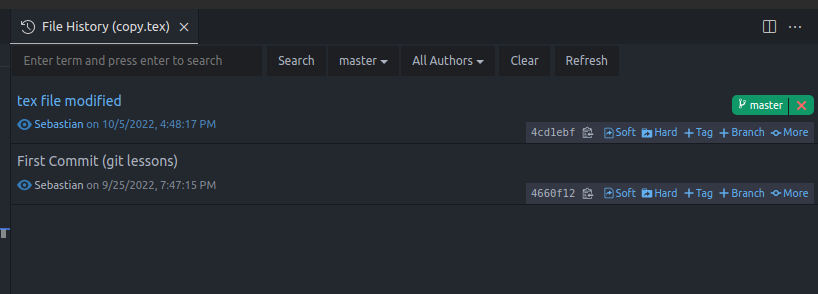
\includegraphics[width=0.6\columnwidth]{Github/Git_f1.png}
\end{figure}


Para cada versión se mostrará el archivo modificado y cómo es su contenido al realizar la confirmación. \\

La siguiente opción es para realizar comparación de ese archivo en esa versión con la actual que está en el espacio de trabajo.

\begin{figure}[H]
    \centering
    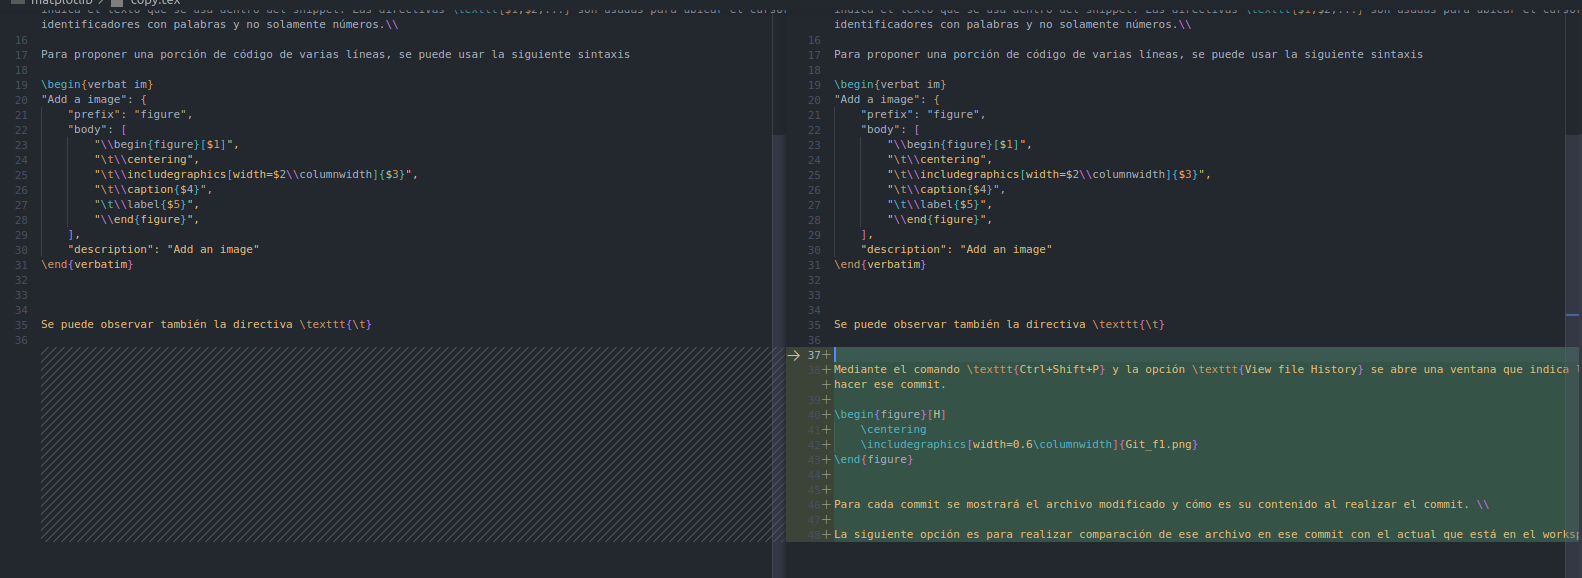
\includegraphics[width=0.6\columnwidth]{Github/Git_f2.png}
\end{figure}

Las siguientes opciones permiten ver la comparación del archivo su versión anterior. Y la última opción permite ver la historia completa del archivo

\subsection{Git Blame}

Esta extensión sirve para realizar revisión línea por línea de por quién, hace cuánto y en qué versión se realizó esa línea de código


\begin{figure}[H]
    \centering
    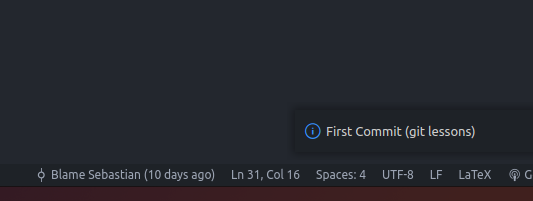
\includegraphics[width=0.6\columnwidth]{Github/Git_f3.png}
\end{figure}


\subsection{Git Lens}

Esta extensión es similar a las anteriores, en que ayuda a verificar las identidades de las personas que están modificando archivos, muestra línea por línea información del autor, y versión de la línea en cuestión.  

\section{Fundamentos de Git: cómo funciona por dentro}

\subsection{Crear un nuevo repositorio}

La sentencia primaria y básica para inicializar un nuevo repositorio es \\

\texttt{git init} \\

Este comando se realiza dentro de la carpeta en la que se desea realizar el repositorio. Una vez creado el repositorio, se pueden añadir las carpetas correspondientes dentro. Al crearse el repositorio, se crea una carpeta oculta llamada \texttt{.git} de manera automática.

dentro de esta carpeta tenemos diferentes carpetas y archivos. Uno de ellos es el archivo \texttt{config}, en este archivo tenemos una serie de cadenas que nos indica las configuraciones que tiene el repositorio. El siguiente es un ejemplo de un archivo de configuración:
\begin{verbatim}
[core]
        repositoryformatversion = 0
        filemode = false
        bare = false
        logallrefupdates = true
        ignorecase = true
[remote "origin"]
        url = https://github.com/JhoAraSan/Process.git
        fetch = +refs/heads/*:refs/remotes/origin/*
[branch "master"]
        remote = origin
        merge = refs/heads/master
\end{verbatim}

Otro archivo es el de descripción \texttt{description}, el cual se puede editar para añadir una descripción al repositorio. Finalmente el archivo \texttt{HEAD}, el cual puede arrojar la siguiente cadena:
\begin{verbatim}
ref: refs/heads/master
\end{verbatim}
Más adelante se dará la explicación correspondiente a este archivo. \\
 Git tiene su propio sistema de archivos; en este sistema de archivos git guarda o almacena objetos, y estos objetos son guardados dentro de la carpeta correspondiente \texttt{objects}.

 \subsection{Objetos en Git}

 En git existen cuatro tipos de objetos:
 \begin{verbatim}
Blob
Tree
Commit
Annotated Tag

 \end{verbatim}
Estos cuatro objetos son los suficientes para poder realizar todo el seguimiento de los archivos del repositorio.
\subsubsection{Blob}
Este es el tipo de objeto en el que git guarda \textbf{archivos}. Todo tipo de archivos con la extensión que sea. Cualquier tipo de archivo serpa guardado como un blob. 
\subsubsection{Tree}
Este es el tipo de objeto en el que git almacena la información sobre los directorios. Dicho de otra fforma, un objeto Tree es una representación de una carpeta o un directorio.
\subsubsection{Commit}
A través de este tipo de objeto, Git es capaz de almacenar diferentes versiones de uno o varios archivos a través del tiempo.
\subsubsection{Annotated Tag}
Este objeto es esencialmente un texto que está apuntando a un commit versión específica. \\

Para poder gestionar o administrar objetos en git se usan los comandos de git de bajo nivel:

\texttt{git hash-object} Con esre comando podemos crear nuevos objetos con la estructura de git.
\texttt{git cat-file} Con este comando se pueden leer los objetos git.
\texttt{git mktree} con este comando se puede crear un nuevo objeto de tipo Tree 

A manera de ejemplo, si colocamos un texto string cualquiera mediante el siguiente comando:

\begin{verbatim}
echo "Hello, Git" | git hash-object --stdin -w
\end{verbatim}

Vamos a obtener como salida un hash, además de que se creará el objeto correspondiente en la carpeta objects; la carpeta será los dos primeros caracteres del hash, y dentro habrá un archivo con el resto de caracteres del hash. Solamente se crea el objeto, el repositorio seguirá estando vacío. Importante remarcar que el hash retornado es el hash del string que le metimos de entrada.

\subsection{JSON}

Las siglas significan "JavaScript Object Notation". Es un formato que permite el intercambio de datos entre diferentes servidores. Como ejemplo, podemos extraer datos mediante una API desde un servidor a una página web. La siguiente es un ejemplo de una estructura JSON:

\begin{verbatim}
{
    "id": "12345667",
    "name": "Mike",
    "age": 25,
    "city": "New York",
    "hobbies": ["Skate", "Running"]
}
\end{verbatim}

Siempre será recomendado que las llaves en un archivo Json sean únicas. La estructura de datos que hay en git es muy similar a JSON; Git tambien almacena nombres "llave" y valores. Las "llaves" en git son los hashes de cada objeto. En git, el hash generado (el cual es equivalente a la key) es función o depende del valor.

\subsection{Hash}

 Al realizar el comando de la seccion anterior, vimos que ek string \texttt{"Hello, Git"} generó un hash \texttt{b7aec520dec0a7516c18eb4c68b64ae1eb9b5a5e}. Esto significa que se aplicó una funcion hash al string o al dato ingresado. \\

 Una función hash es una función que toma una entrada de cualquier tamaño (longitud) y tiene una salida de un tamaño fijo. Es importante también notar que el hash es una funccióon unidireccional, es decir, que si tenemos un hash generado no vamos a poder saber cuál fue la entrada que la generó. Para la misma función hash, la misma entrada siempre va a generar la misma salida. \\

 Las fuciones o algoritmos para generar hashes más importantes son las siguientes:

 \begin{itemize}
     \item MD5 (128 bit)
     \item SHA1 (160 bit)
     \item SHA256 (256 bit)
     \item SHA384 (384 bit)
     \item SHA512 (512 bit)
 \end{itemize}

 El algoritmo usado por git para generar sus hashes es \texttt{SHA1}.

 Cada caracter de 4 bits de longitud está está en formato hexadecimal. Por tanto, un hash de git tiene una longitud de 40 caracteres hexadecimales. \\

 Dado lo anterior, surge la pregunta de cuantos archivos diferentes podemos guardar en el mismo repositorio.

 La cantidad total de hashes diferentes es $16^{40} \approx 1.46 \ 10^{48}$. Por otro lado podemos havernos la pregunta de cual es la posibilidad de que dos archivos diferentes produzcan el mismo hash? \\

 La probabilidad de encontrar un hash específico es $\frac{1}{16^{40}} \approx 6.84 \ 10^{-49}$. Por tanto para saber la probabilidad de que dos archivos produzcan el mismo hash, tenemos \\

 \begin{equation*}
 P = \frac{1}{16^{40}}  \frac{1}{16^{40}} = \frac{1}{16^{80}} \approx 4.68 \ 10^{-97}
 \end{equation*}

Como elemento adicional, tenemos que la probabilidad de que teniendo $n$ archivos diferentes, dos de ellos generen el mismo hash, es el siguiente:

\begin{equation*}
P = \frac{(2^{160}-n)!(2^{160})^{n-1} - (2^{160} - 1)! }{ (2^{160}- n)! \ 2^{160(n-1)} }
\end{equation*}

Para que haya una probabilidad de 1 de que haya una colision de hash es necesario que en un repositorio hayan más archivos que número diferente de hashes. 

\subsection{Exploración de objetos de git mediante \texttt{cat}}

Recordemos que todo objeto de git tiene su correspondiente hash. Podemos usar el comando \texttt{git cat} para obtener información de cualquier objeto. Las opciones del comando son: 

\texttt{git cat-file -p <hash>} Retorna el contenido del objeto. \\
\texttt{git cat-file -t <hash>} Retorna el tamaño del objeto. \\
\texttt{git cat-file -s <hash>} Retorna el tipo del objeto. El tamaño lo retorna en bytes. \\

\subsection{Creación de objetos mediante comandos de git}

el comando \texttt{git hash-object} se usa para crear nuevos objetos, luego tenemos varias opciones adicionales:
\begin{verbatim}
echo "Hello, Git! | git hash-object --stdin -w
\end{verbatim}

La promera opvion es para romar la intrada como entrada estandar, la segunda es importante porque es la que hace se cree el objeto. También podemos crear objetos en git basados en archivos locales:

\begin{verbatim}
git hash-object <filename> -w
\end{verbatim}

Una cosa importante de notar es que en git cuando almacenamos archibos del tipo blob, estos objetos no tienen un nombre de archivo. Como se podrá ver en los anteriores comandos, ninguno de ellos retorna el nombre del archivo puesto que este no se almacena. Otra cosa importante de notar es que tanto el tamaño como el tipo de objeto se almacenan dentro del mismo hash. La estructura con la que lo hace es la siguiente:

contenido + tipo de objeto + tamaño del objeto = hash.  Entre el tipo de objeto más tamaño, y el contenido del objeto hay un delimitador. En esencia, el hash se genera a partir de lo siguiente:

\begin{verbatim}
blob 11\0Hello
\end{verbatim}

El delimitador es \texttt{$\backslash$0}, antes del delimitador tenemos el tamaño que para el ejemplo es 11 bytes, y antes el tipo de objeto seguido de un espacio. Luefo del delimitador está el contenido del archivo. 

\subsection{Tree}

Este tipo de objeto es el que representa las direcciones y los directorios.  Un objeto Tree puede tener tanto blobs como otros trees. La estructura es la misma de los demás objetos (tipo, tamaño, delimitador y contenido). En este caso el contenido será diferencial al de un blob: 

\begin{verbatim}
100644 blob 57537e1d8fba7d80c5bcca8b04e49666b1c1790f .babelrc
100644 blob 602c57ffb51af99d6f3b54c0ee9587bb110fb990 .flow config
040000 tree 80655da8d80aaaf92ce5357e7828dc09adb00993 dist
100644 blob 06a8a51a6489fc2bc982c534c9518f289089f375 package.json
040000 tree fc01489d8afd08431c7245b4216ea9d01856c3b9 src
\end{verbatim}

Como podemos ver un tree puede contener blobs y más trees, tenemos tres secciones importantes: el primer número representa los permisos, el segundo es el tipo de objeto, luego va el hash, y por último el nombre o directorio.

\subsection{Permisos de objetos de git}

El primer número representa los permisos de los objetos de Git, estos permisos se pueden ver en la siguiente lista.

\begin{verbatim}
040000 Directorio
100644 Archivo regular no ejecutable
100664 Archivo de escritura de grupo no ejecutable normal
100755 Archivo ejecutable regular
120000 Link simbólico
160000 Gitlink
\end{verbatim}

La razón de que existan estos permisos es porque los repositorios de git deben ser independientes de cualquier sistema de archivos del SO en el que está.

\subsection{Creación de objetos Tree}

Teniendo un ejemplo de dos objetos blob, cada uno con su respectivo hash, podemos crear un archivo del tipo tree que nos proporcione apuntadores para cada uno de los blobs y que nos proporcione la información de los nombres de los archivos de los blobs. Si los dos archivos blobs tienen los siguientes hashes 

\begin{verbatim}
284a47ff0d9b952bab8ccbae29b97b5beb700e82
814d2ecd90a29b25b12880623d82e727f9a650cb
\end{verbatim}

Los cuales representan los archivos \texttt{file1.txt} y file \texttt{file2.txt}; en este caso, el contanido del tree será el siguiente:

\begin{verbatim}
100644 blob 284a47ff0d9b952bab8ccbae29b97b5beb700e82 file1.txt
100644 blob 814d2ecd90a29b25b12880623d82e727f9a650cb file2.txt
\end{verbatim}

Para crear un nuevo tree usamos el comando \texttt{git mktree}, primero creamos un objeto del tipo texto con el contenido de arriba y lo guardamos en cualquier carpeta. 

\subsection{Tres pilares importantes}

Dentro de los repositorios tenemos y podemos identificar tres áreas fundamentales: directorio de trabajo (working directory), staging area o index, y git repository. 

El staging area que también es llamado index es el área responsable de preparar los archivos para ser insertados en un repositorio limpio, y del mismo modo, prepara los archivos tomados del repositorio para ser puestos en el directorio del trabajo. El proceso en el que los archivos pasa por el area de staging es siempre obligatorio. Es el puente entre el directorio de trabajo y el repositorio de git. Si un objeto tree está representando el nombre de dos objetos blob, significa que esta representando un directorio raíz. Es decir que se hace necesario describir otro tree que represente una carpeta con su respectivo nombre en la que estén alojados los dos archibvos blob.

\texttt{git ls-files -s} es un comando que sirve para listar los archivos que se encuentran en el staging area. Si queremos enviar cualquier objeto tree desde el repositorio de git hasta el area de staging, usamos el comando \texttt{git read-tree <hash>}.

\subsection{Git checkout index}

Teniendo los dos objetos blob creados a mano y el objeto tree también creado a mano con los nombres de los anteriores blobs, y también ateniendo estos dentro del staging area, se pueden añadir dentro del directorio de trabajo, que corresponde a la carpeta física (dentro del sistema de archivos de cada SO) en la que se ven los archivos. Esto se hace con el siguiente comando: \texttt{git checkout -index -a}. Con la opción \texttt{-a} decimos que agrege todos los archivos.

\section{Operaciones básicas de Git}

\subsection{¿Qué es commit?}

Uno de los cuatro tipos de objetos principales es el denominado "commit". Lo primero de todo es que \texttt{commit} tiene la misma estructura que los otros tipos de objetos; es decir, que contiene la estructura de los objetos en git: un hash del tipo sha1 que consiste es tipo de objeto + tamaño + delimitador + contenido. \\

La diferencia esta en que el contenido de un commit es el siguiente: nombre de autor, correo de autor, descripción de la versión, y como opcional, la versión padre. La confirmación de versión (commit) sirve esencialmente para guardar diferentes versiones de los proyectos. \textbf{Cada commit es una versión diferente del proyecto}.

La siguiente imagen muestra cómo son los apuntadores de cada objeto de git:

\begin{figure}[H]
    \centering
    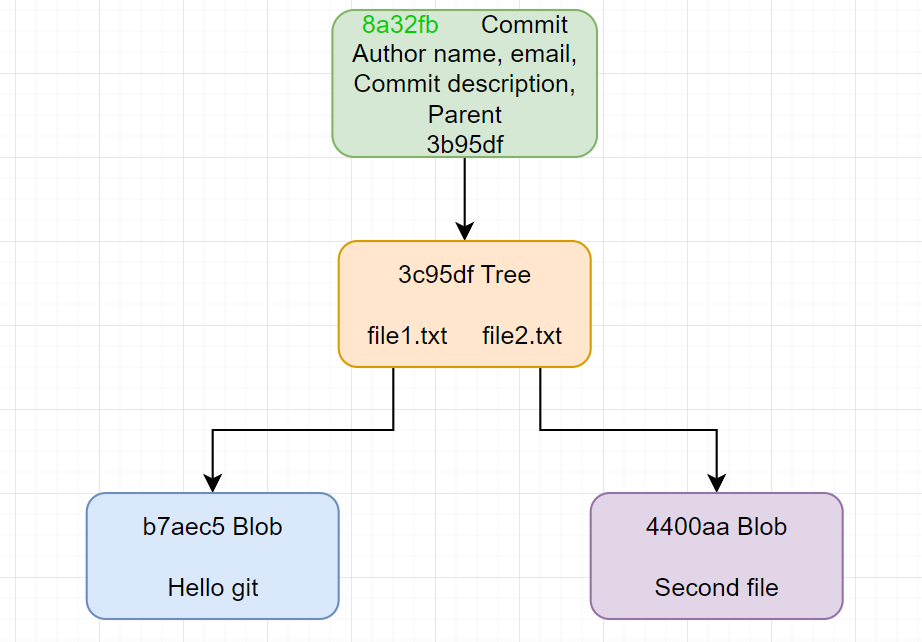
\includegraphics[scale=0.5]{Github/Git_f4.png}
\end{figure}

Como se puede ver, el archivo de versión (commit) es una especie de envoltorio para el objeto tree, y tiene un apuntador hacia el tree. Cada uno de los commits, puede ser llevado al directorio de trabajo para ver esa versión del proyecto. Los siguientes comandos sirven para establecer en git el nombre y dirección de correo electrónico:

\begin{verbatim}
git config --global user.name <name>
git config --global user.email <Email> 
\end{verbatim}

Y para leer la configuración establecida, usamos el siguiente comando: \texttt{git config --list}

\subsection{Creación de las primeras versiones}

En primer lugar, debemos estar pendientes de cuál es el estado del repositorio.

\begin{verbatim}
git status
\end{verbatim}

Con el comando anterior podemos ver los cambios realizados para ser confirmados. También podemos ver si hay algún cambio sin seguimiento para añadir y posteriormente ser enviados/confirmados. 

Una vez tengamos listos los cambios realizados para enviar, usamos el comando \texttt{git commit -m "comment"}. Con la opción \texttt{-m} podemos asignar un comentario a la versión. Es muy importante tener en cuenta que cuando hacemos confirmación de versión, estamos enviando información del 'staging area' al 'git repository', y cuando hacemos el proceso contrario (desde 'staging area' a 'working directory'), el proceso se llama 'checkout'.

El commit como archivo hash contiene lo siguiente:

\begin{itemize}
    \item tree (es el hash del tree principal al que apunta el commit)
    \item parent (es el hash del commit anterior)
    \item Usuario autor de los cambios  
    \item Usuario que confirmó el cambio
    \item Comentario
\end{itemize}

\subsection{Comandos básicos de git}

\begin{itemize}
    \item \texttt{git status}
    \item \texttt{git add} con este se agregan aarchivos al area de staging
    \item \texttt{git commit} con este se se escriben los cambios al repositorio ya como objetos
    \item \texttt{git log} con este se muestra el historial de cambios o commits
    \item \texttt{git checkout} este comando sirve para poner en el directorio actual (working directory) un commit o un branch específico.
    \item \texttt{git cat-file -p <hash>} Con este comando, como se mostró arriba, se visualiza el contenido del archivo correspondiente al hash ingresado.
    \item \texttt{git ls-files -s} Lista todos los archivos (blob) indicando el directorio donde están e indicando su hash.
\end{itemize}



Cuando se agrega un nuevo archivo al directorio, los archivos pueden tener cuatro estados diferentes:
\begin{itemize}
    \item Untracked
    \item Modified
    \item Staged
    \item Unmodified
\end{itemize}


Si un archivo recién creado se adiciona al directorio, directamente está en el estado "untracked". En la siguiente figura se puede observar cómo va cambiando el estado de los archivos.


\begin{figure}[H]
    \centering
    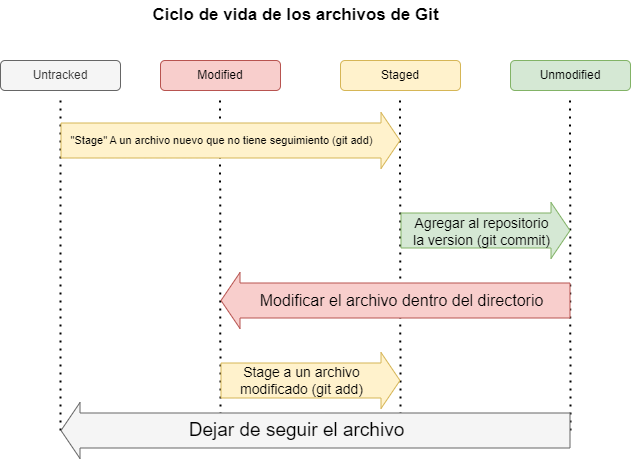
\includegraphics[scale=0.65]{Github/Git_f5.png}
\end{figure}

Para listar los archivos que están dentro del staging area, se usa el comando \texttt{git ls-files -s}. Al agregar archivos al área de staging, tenemos varis opciones

\begin{itemize}
    \item \texttt{git add <name>} Agrega el archivo especificado a la zona de preparación.
    \item \texttt{git add -A} Agrega todos los archivos modificados, eliminados y nuevos al área de preparación. La opción -A incluye archivos en subdirectorios.
    \item \texttt{git add .} solo incluye los archivos en el directorio actual.
    \item \texttt{git add -u} Agrega todos los archivos modificados y eliminados al área de preparación, pero no los nuevos.
    \item \texttt{git add -p} Abre una sesión interactiva que permite agregar solo partes seleccionadas de los cambios realizados en un archivo.
\end{itemize}

Además podemos quitar archivos del area de preparación, mediante el comando \texttt{git rm --cached <name>}, esta última opción sirve para quitar un archivo en específico. \\

Una de las propiedades importantes de ver es que cuando realizamos un commit, este tiene un apuntador a su commit padre, es el hash de su commit padre. Según el tipo de commit este tendrá uno u otro commit padre (más adelante se verá que para pull requests pueden haber punteros distintos.

\subsection{Historial de un archivo}

Un comando útil para analizar la historia de un archivo en nuestro repositorio es el siguiente

\begin{verbatim}
    git log --pretty=oneline <archivo_con_su_ruta>
\end{verbatim}

Este comando retorna una lista de hashes que corresponden a los commits que han modificado dicho archivo:

\begin{verbatim}
13bde112178bbf94d9f83a2a14397c14d8cb973b UpdateBrowser
288cb6fee465de9e1bf682c7b47a25c4c75dd9e7 UpdateBrowser
2f7e1498f72e5d77b2773938f8516dd4c576b922 UpdateDictJson
23835e0a0d35796e708c50cfc71c523ef1b941d5 UpdateDictJson
f9dd3785bbc39a5e1ae9f8fed003f7b696f17f6b Se cambia apertura de navegador para form OVH
e1b1a7f0632ef745d02749468aa02eee016e62f9 Merge branch 'test2' of https://github.com/JhoAraSan/Process into test2
863641d145bdff2d4546a9b8f0328afed95d74ac Update code
47cf1a72d0ee58077a61558072c0866c46295547 cloudflare form bus ixed
673268edaff5d407e7de309c14e8a81829adf137 update
bdc232b7cb40c41c70eacfe7182d510145f26ce2 check bug
.
.
.
\end{verbatim}

Como se puede ver, se muestra el hash del commit y a continuación se muestra el comentario realizado. El primer commit en la lista es el más reciente. El último de la lista será el commit que creó el archivo. 

De forma alternativa, se puede ver solamente el commit creador del archivo en cuestión mediante el comando

\begin{verbatim}
git log --pretty=oneline --diff-filter=A -- .\Consola_3000\Consola3000.py
\end{verbatim}

El cual devuelve

\begin{verbatim}
04bf774da85b9db1a059da4111887240ad2b3d4e renombramiento de carpeta a sugerencia de Sebastian
\end{verbatim}

\section{Las ramas}

Como introducción a la sección, recordemos la capacidad de llevar un commit (screenshot de una versión del proyecto) al directorio actual. Esto se realiza mediante el comando "git checkout". En otras palabras, es algo así como saltar hacia una versión especifica del proyecto. \\

Una definición general de lo que es una rama de github, es que es una referencia textual a un commit. Las siguientes son características de las ramas en git:

\begin{enumerate}
    \item La rama por defecto es la master.
    \item En un mismo repositorio pueden existir varias ramas.
    \item Los apuntadores a todas las ramas se localizan en \texttt{.git/refs/heads}
    \item Cada rama maneja sus propios commits.
    \item El puntero de la rama se mueve automáticamente después de cada nuevo commit.
    \item Para cambiar de branch se usa el comando \texttt{git checkout <branch>}
\end{enumerate}

El puntero de la rama será el último commit realizado en dicha rama, el archivo es un texto que contiene el hash de dicho commit.

\subsection{HEAD}

El concepto de head es util para especificar al sistema cuál es la rama en la que me encuentro actualmente. Básicamente HEAD es el apuntador que apunta hacia la rama/commit \textbf{actual}. Solamente existe un solo HEAD en cada proyecto.

\begin{enumerate}
    \item El puntero se guarda en \texttt{.git/HEAD}
    \item El Puntero por defecto es \texttt{refs:/heads/master}
    \item Para cambiar la referencia a una rama específica se usa \texttt{git checkout <branch>}
    \item Para cambiar la referencia a un commit específico se usa \texttt{git checkout <sha1>}
\end{enumerate}

\begin{figure}[H]
    \centering
    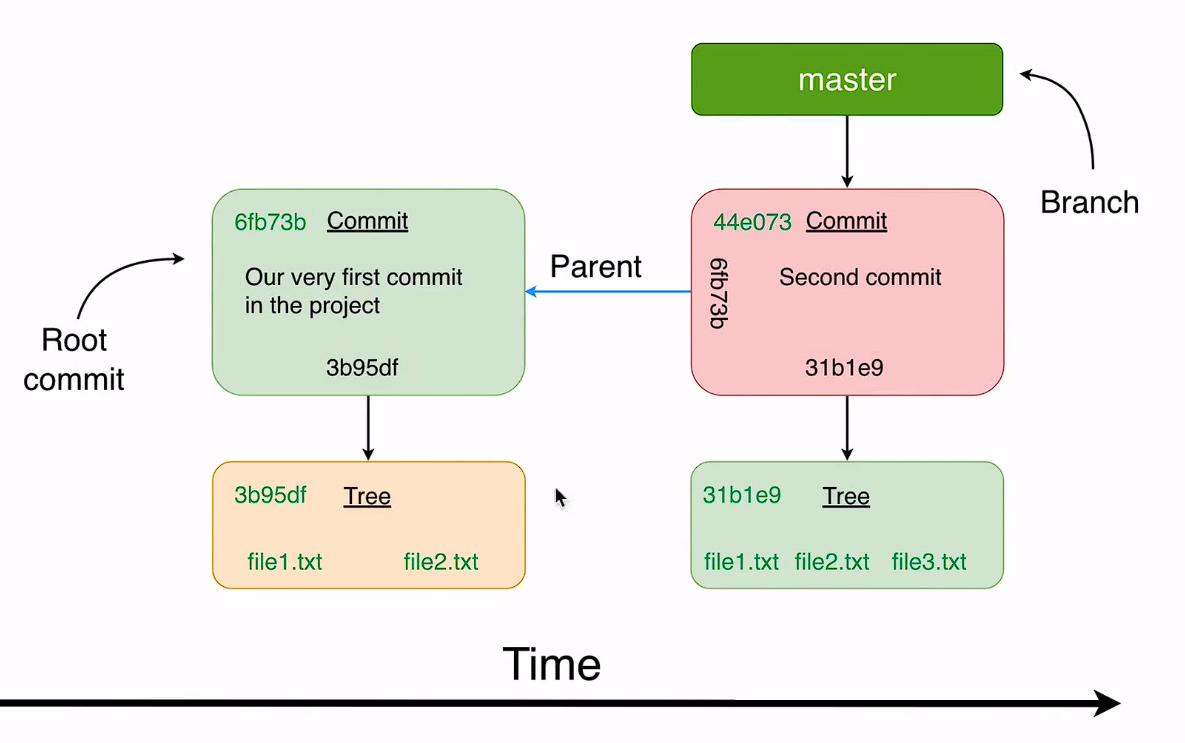
\includegraphics[scale=0.4]{Github/Git_f6.png}
\end{figure}


Cada vez que se crea una nueva rama en un repositorio de Git, se crea una referencia a la cabeza (HEAD) de esa rama en el sistema de archivos de Git. Esta referencia se guarda en el directorio \texttt{.git/refs/heads/} dentro del repositorio.


Para la administración de las ramas disponemos de los siguientes comandos:

 \begin{itemize}
     \item \texttt{git branch} Lista todas las ramas locales
     \item \texttt{git branch <name>} Crea una nueva rama
     \item \texttt{git checkout <branch>} Se dirige a la rama especificada
     \item \texttt{git branch -d <name>} Borrar la rama especificada
     \item \texttt{git branch -m <old> <new>} Renombrar la rama especificada
 \end{itemize}

 Un comando muy útil para crear una rama nueva y dirigirse directamente a ella es la siguiente:

 \begin{verbatim}
git checkout -b <branch name>
 \end{verbatim}

\subsubsection*{Ejemplo}

Para un repositorio de un proyecto cualquiera como ejemplo vamos a la carpeta \texttt{.git/refs/heads}.

Si se lista el contenido del directorio se obtiene la siguiente salida

\begin{verbatim}
    Directory: C:\Users\seb-c\OneDrive\Documentos\Project_Process\Process\.git\refs\heads

Mode                 LastWriteTime         Length Name
----                 -------------         ------ ----
la---           3/25/2023  3:49 PM             41 master
la---            9/6/2023  9:31 AM             41 speechGen
la---           9/10/2023  4:00 PM             41 test2
\end{verbatim}

El cual muestra que en el repositorio de ejemplo hay tres ramas: master, speechGen y test2. Si queremos ver el contenido del archivo \texttt{speechGen} se obtiene

\begin{verbatim}
866c48dd5d96c7ba7ae730dbd3dc85896bc6b576
\end{verbatim}

Este es el hash correspondiente al \textbf{último} commit de esta rama. De aquí se puede concluir que la rama puede verse como un apuntador hacia el commit. 

Para ver dónde se guarda el apuntador general HEAD hacia la rama (o commit) en el que se está actualmente. Vamos al directorio que guarda el puntero: 

\begin{verbatim}
cd .git
cat HEAD
\end{verbatim}

Se obtiene lo siguiente


\begin{verbatim}
ref: refs/heads/test2
\end{verbatim}

El cual indica que en el momento de realizar el comando, el usuario estaba en la rama \texttt{test2}

\section{Repositorios remotos}

En esta sección se describirán algunas características no antes vistas sobre los procesos asociados a los repositorios remotos.

\subsection{git diff}

Este es un comando que puede ser útil para ver y evidenciar las diferencias entre un archivo modificado su anterior versión dentro de la consola. Al usar el comando podemos ver el hash provisional del nuevo archivo (el que tendria si se realiza el commit), las líneas agregadas- quitadas-modificadas.

\section{Fusión o combinación de ramas}
Es importante tener clara la perspectiva de dónde está apuntando \texttt{HEAD}. De ello depende la información que vamos a obtener al llamar al comando \texttt{git log}. Si estamos visualizando commits anteriores, ese commit será el actual para la vista que tengamos en el momento. \\
Ahora teniendo en cuenta lo anterior, suponemos que hemos creado una rama para agregar cualquier especificación; hemos creado esa rama desde la rama principal. Luego hemos realizado cambios en dicha rama y hemos confirmado dichos cambios. Posteriormente volvemos a cambiar la vista hacia la rama principal y \textbf{desde esta rama traemos o unimos los cambios realizados en la rama secundaria}; ese es el proceso de fusión o combinación de ramas. 

\begin{verbatim}
git merge <feature-branch>
\end{verbatim}
En esencia, cuando hacemos la fusión de ramas, lo que estamos realizando es un cambio del apuntador de la rama hacia la que fusionamos (la principal) para apuntar ahora al último commit realizado en la rama que estamos trayendo. Este caso aplica cuando en la rama principal no hay cambios después de haber creado la rama secundaria.\\
\begin{figure}[H]
    \centering
    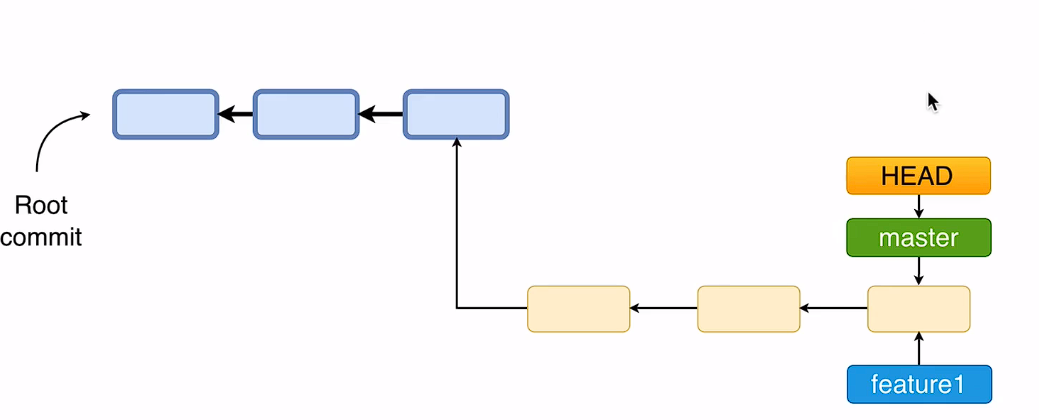
\includegraphics[scale=0.5]{Github/Git_f7.png}
\end{figure}
Supongamos ahora que tenemos nuestra rama principal, creamos una rama para trabajar en características secundarias, pero al mismo tiempo también realizamos cambios en la rama principal. Si en este momento queremos hacer una fusión de las ramas, ya no podemos simplemente cambiar el puntero de la rama principal; ahora es necesario realizar una fusión de 3 direcciones. \\
En la fusión de tres direcciones tenemos tres versiones importantes: la versión ancestro, que corresponde a la última versión en común que tienen las dos ramas a unir; la última versión de la rama secundaria y la última versión de la principal.
Como en la fusión anterior, también se debe ir a la versión de la rama receptora; se crea una nueva versión de fusión en esta rama; \textbf{dicha versión tendrá como versiones padres la última de la rama receptora y la última de la rama secundaria}. Si no existen conflictos entre archivos que se hayan modificado en ambas ramas, simplemente la nueva versión combinará los archivos nuevos.\\

\begin{figure}[H]
    \centering
    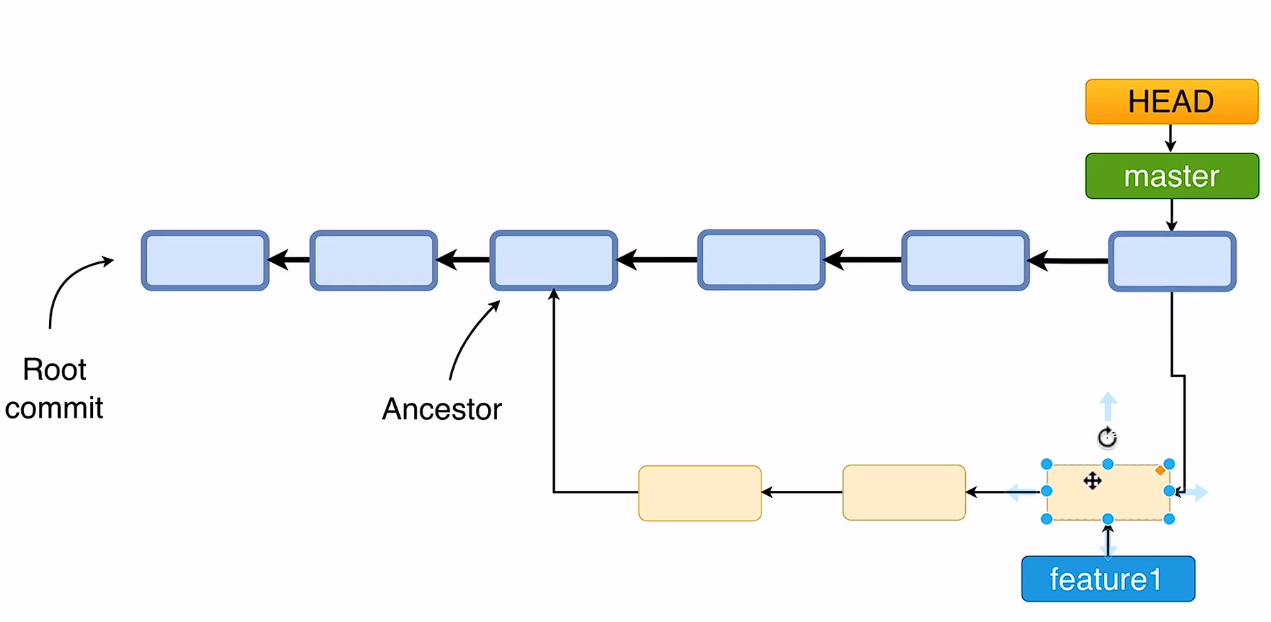
\includegraphics[scale=0.3]{Github/Git_f8.png}
\end{figure}
Una vez realizado este proceso, se puede borrar la rama secundaria, lo cual significa borrar el apuntador de la rama, las versiones permanecen. 

\subsection{conflictos de fusión}

Los conflictos ocurren cuando se intenta fusionar dos ramas y en ambas se ha modificado el mismo archivo. Estos conflictos siempre deben ser arreglados manualmente. Si intentamos unir dos ramas y se generan conflictos, el estado actual del repositorio cambiará a tener dos caminos sin fusionar. Git le pedirá al usuario que corrija los conflictos y que confirme dichos cambios. Están las opciones de dejar los cambios de la rama principal, dejar los cambios de la rama secundaria, o de dejar ambos cambios. \\

Algo interesante de observar, es que en este momento se habrán creado tres objetos blob diferentes en el staging area. tres objetos que tienen el nombre del archivo que contiene el conflicto. El primero corresponde a la versión ancestro de ambas ramas, el segundo corresponde a la modificación de la rama principal, y el ultimo corresponde a la modificación de la rama secundaria. Existen varias formas de resolver estos conflictos; el primero se puede hacer mediante la consola: \\

Abrimos el archivo que contiene los conflictos mediante \texttt{nano} por ejemplo y seleccionar manualmente cuál de la(s) líneas van a ser conservadas. guardar el archivo y de esta manera el o los conflictos habrán sido resueltos. También se tiene a opción de incluso volver a modificar el archivo si ninguna de las dos versiones es la que queremos. Finalmente cuando las modificaciones sean las deseadas, podremos concluir la fusión de las ramas mediante la confirmación (commit). 

\section{Comandos para los repositorios remotos}

Dentro de los comandos más importantes para la clonación de los repositorios remotos, los siguientes son los más importantes:

\subsection{Git push}

Añadido a las tres áreas de los repositorios, tenemos un área adicional que corresponde al repositorio remoto. El primer comando envía toda la información desde el área de repositorio local y lo envía directamente al repositorio remoto. Solamente los cambios que están confirmados son los que efectivamente se ven reflejados en el repositorio remoto. 

\begin{figure}[H]
    \centering
    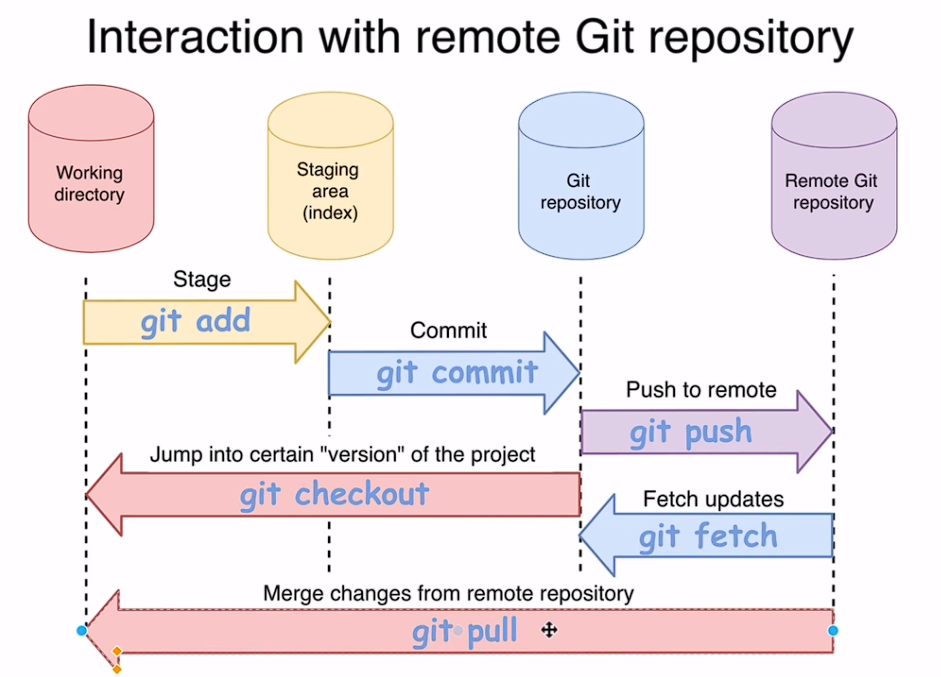
\includegraphics[scale=0.5]{Github/Git_f9.png}
\end{figure}

\subsection{Git fetch y pull}

Una vez el repositorio está actualizado, y es necesario pasar esa información al repositorio local, se pueden hacer dos comandos, el primero es \texttt{git fetch}: este comando es para enviar toda la información del repositorio remoto al repositorio local, pero sin enviarlo al área del directorio de trabajo. Por su parte, si queremos enviar directamente la información del repositorio remoto al directorio de trabajo usamos el comando \texttt{git pull}. \\

Para entender un poco la diferencia entre los dos comandos, supóngase que se crea una nueva rama en el repositorio remoto. Después de realizar \texttt{git fetch} dicha rama será creada en el repositorio local. En otras palabras, con git fetch básicamente estoy actualizando la información del repositorio remoto en mi repositorio local.

Por su parte, el siguiente ejemplo muestra el funcionamiento de \texttt{pull}:

\begin{enumerate}
    \item Se clona el repositorio remoto
    \item Se hace \texttt{checkout} a la rama master en el repositorio local
    \item Se realizan cambios y se confirman en la rama master del repositorio remoto
    \item Después de realizar \texttt{git pull} el repositorio local extraerá los cambios del remoto.
    \item Git realiza la fusión de la rama master en el repositorio local 
    \item Tanto el área de stagig como el directorio de trabajo se actualizan automáticamente luego de la fusión.
\end{enumerate}

Cuando uno clona un repositorio remoto en uno local, git automaticamente crea un enlace entre ambos repositorios. Por defecto para el repositorio local, el nombre del repositorio remoto es \texttt{origin}. 

Siempre que se clona un repositorio, git solamente crea una rama local con el mismo nombre de la rama por defecto del repositorio remoto. Por tanto, si tenemos dos ramas en el repositorio remoto, y clonamos este repositorio, en nuestro repositorio local solamente habrá una rama que es la rama principal del repositorio remoto. Para poder traer una rama remota que no es la principal a nuestro repositorio local, solamente necesitamos hacer un checkout a dicha rama, de esta forma esta rama aparecerá en nuestro repo local.

Para los repositorios remotos, un comando importante y útil puede ser el siguiente \texttt{git remote show origin}. Con este comando podemos ver mucha más información sobre el repositorio remoto como las ramas remotas, las ramas locales, cuáles están configuradas o trackeadas, etc. El siguiente es un ejemplo de la unformación total de un repositorio remoto:

\begin{verbatim}
PS C:\Users\seb-c\OneDrive\Documentos\Project_Process\Process> git remote show origin
* remote origin
  Fetch URL: https://github.com/JhoAraSan/Process.git
  Push  URL: https://github.com/JhoAraSan/Process.git
  HEAD branch: master
  Remote branches:
    master                      tracked
    refs/remotes/origin/clases  stale (use 'git remote prune' to remove)
    refs/remotes/origin/test    stale (use 'git remote prune' to remove)
    refs/remotes/origin/virtual stale (use 'git remote prune' to remove)
    speechGen                   tracked
    test2                       tracked
  Local branches configured for 'git pull':
    master    merges with remote master
    speechGen merges with remote speechGen
    test2     merges with remote test2
  Local refs configured for 'git push':
    master    pushes to master    (up to date)
    speechGen pushes to speechGen (up to date)
    test2     pushes to test2     (up to date)
\end{verbatim}

En este ejemplo "\texttt{stale}" indica que la rama fue borrada del repositorio remoto, y se puede quitar de la lista con el comando \texttt{git remote prune origin}

Por su parte, cuando queremos sincronizar los cambios entre el repositorio remoto y el local, las ramas siempre harán un merge, es decir que se fusionarán y habrá que manejar los posibles conflictos que hayan entre la rama local y su correspondiente remota.  

Para el siguiente ejemplo podemos listar todas las ramas en los repositorios local y remoto:

\begin{verbatim}
git branch -a     

  master
  speechGen
* test2
  remotes/origin/HEAD -> origin/master
  remotes/origin/clases
  remotes/origin/master
  remotes/origin/speechGen
  remotes/origin/test
  remotes/origin/test2
  remotes/origin/virtual
\end{verbatim}

Como se puede ver, la línea \texttt{remotes/origin/HEAD -> origin/master} indica que en el repositorio remoto, la rama por defecto es la master.

\subsection{Ramas rastreadas}

Las ramas rastreadas son todas las ramas del repositorio remoto que tienen su correspondencia con la rama en el repositorio local. En otras palabras, son las ramas que aparecen tanto en el repositorio remoto como en el repositorio local.

Cuando se clona un repositorio remoto, solamente se crea la rama principal en el repositorio local. Estando en repositorio local se realiza el comando \texttt{git checkout} a una rama del repositorio remoto, y en ese momento se crea la rama rastreada. El comando \texttt{git branch -vv} muestra información de las ramas rastreadas:

\begin{verbatim}
git branch -vv

  master    5d42019 [origin/master] Unificando y dejando la verdadera principal
  speechGen 866c48d [origin/speechGen] first ver apps module in window DONE!
* test2     3c3e9ae [origin/test2] Cambio del nombre de la Appstore
\end{verbatim}

Como se ve, se muestra el nombre, el hash y el comentario de las ramas que están rastreadas.

\subsection{Proceso pull}

Para realizar un \texttt{git pull}, se combinan varios conceptos previamente discutidos:

\begin{enumerate}
    \item Rama de reastreo local: Es necesario tener una rama local que esté rastreando una rama remota para poder realizar un \texttt{pull}
    \item Funcionamiento del \texttt{merge}: Es necesario entender cómo funcionan las fusiones. Recordar que puede hacerse con el enfoque de avance rápido o con una fudión de tres vías.
    \item \texttt{git fetch} antes del \texttt{pull}, git efectúa un \texttt{fetch} para obtener todos los cambios desde el repositorio remoto
\end{enumerate}

El proceso de \texttt{git pull} se realiza en dos pasos:\\
Primero se ejecuta un \texttt{git fetch}, que tona todas las actualizaciones del repositorio remoto y las escribe en el repositorio local. Esto incluye todas las nuevas reamas y versiones creadas en el repositorio remoto.

Luego de ejecuta un \texttt{git merge}. Esta fusión es local, es decir, se hace en el repositorio local sin interactuar con el repositorio remoto. Durante este proceso, se utilizan dos ramas: la rama receptora será la rama local y la rama "feature" será la rama remota correspondiente. Git mezclará la rama remota en la rama local. \\
Es relevante notar que Git usa un término especial, "Fetch Head", en lugar del nombre de la rama remota durante este proceso. Como limitación, \texttt{git pull} actualiza solo la rama local que está actualmente en uso. No afecta ninguna otra rama local.


\subsection{Fetch head}

Pongamos un ejemplo: sea un repositorio tal que al revisar las ramas tanto locales como remotas obtenemos el siguiente resultado:

\begin{verbatim}
git branch -a

*   feature-1
    master
    remotes/origin/HEAD -> origin/master
    remotes/origin/master
\end{verbatim}

Vemos que tenemos las dos ramas remotas master y feature-1 con sus correspondientes ramas locales. Si hacemos el siguiente código

\begin{verbatim}
git branch -vv
*   feature-1   ccc9d7b [origin/feature-1] 
    master      f38cf54 [origin/master]
\end{verbatim}

Vemos nuevamente la correspondencia entre las ramas. Escribiendo el comando \texttt{fetch} y luego \texttt{pull} tenemos lo siguiente:

\begin{verbatim}
git fetch -v

From https://github.com/yo/myrepo
 = [up to date] feature-1   ->  origin/feature-1
 = [up to date] master      ->  origin/master

git pull
Already up to date

 
git pull -v
 
From https://github.com/yo/myrepo
 = [up to date] feature-1   ->  origin/feature-1
 = [up to date] master      ->  origin/master 
 Already up to date
 \end{verbatim}

Con lo anterior podemos ver que pull siempre hace fetch antes de hacer algunos cambios adicionales para 
intentar fusionar las ramas.



Si vemos los archivos que están dentro de la carpeta \texttt{.git} podremos ver que hay un archivo llamado \texttt{FETCH\_HEAD}, cuyo contenido sería el siguiente


\begin{verbatim}
cat FETCH_HEAD
73acf27141929dd1f890236317cb54009914c35a                branch 'test2' of https://github.com/JhoAraSan/Process
629fab88a1c5954a9389c827f0e7b4829ce734ba        not-for-merge   tag '1' of https://github.com/JhoAraSan/Process
\end{verbatim}

Este contenido corresponde a las ramas que están en el repositorio remoto. Si cambiamos de rama, al hacer este mismo comando, veremos en primer lugar la rama que está actualmente. Cuando hacemos git pull, Git primero ejecuta "git fetch". Despues del fetch se actualiza la lista de .git/FETCH\_HEAD y la primera rama de esta lista será la rama actual. 
finalmente Git ejecuta \texttt{git merge FETCH\_HEAD} que busca la primera rama en el fetch head sin la etiqueta "not-for-merge" y la fusiona con la rama local actual. 

\subsection{Git pull con modificacion de repositorio remoto}

Si despues de hacer \texttt{git pull} el repositorio remoto es modificado, se crea un nuevo commit en el repositorio remoto. Git actualiza el repositorio y realiza la actualización del apuntador en el repositorio local, del commit antiguo al nuevo commit. \\

Ahora supongamos que se realizan cambios tanto en el repositorio remoto como en el repositorio local, y queremos traer o hacer pull al repositorio remoto. Tengamos en cuenta que al revisar con \texttt{git log}, veremos el último commit que acabamos de hacer, y anterior a ese veremos el último commit sincronizado; el que se supone que es el último commit del repositorio remoto. Sabemos que esta es una información falsa, pues este commit está desactualizado. Mediante el comando \texttt{git fetch}, vamos a actualizar la información del cambio realizado en el repositorio remoto, aunque Git ya creó los objetos dentro del repositorio local, estos aún no se ven en el directorio de trabajo porque aún no se ha fusionado con la rama local.

Después de esto podemos fusionar el cambio remoto con el cambio local. Mediante \texttt{git merge FETCH\_HEAD} 

\subsection{Subida de cambios al repositorio remoto}

Ahora que tenemos cambios en el repositorio local que están ausentes en el repositorio remoto, es hora de poner la operación push en acción. Recordar siempre que es necesario tener permisos de escritura. Una vez estén sincronizados los repositorios, podemos ver que los apuntadores de los repositorios local (que está en la carpeta \texttt{.git/refs/head}) y la remota (que está en la carpeta \texttt{.git/refs/remotes/origin}) tienen el mismo c0ommit de destino. \\

Si necesitamos crear una rama nueva, los pasos a realizar para que también se vea reflejada en el repositorio remoto es lo siguiente:

\begin{enumerate}
    \item Se crea la nueva rama local mediante \texttt{git checkout -b nueva}
    \item Se hacen los cambios correspondientes.
    \item Se confirman los cambios con \texttt{commit}
    \item Se sube la nueva rama al repositorio remoto con el comando \texttt{git push -v -u origin feature-2}
\end{enumerate}

\subsection{De rama local a rama nueva remota}

Cuando se crea una rama nueva en el repositorio local y se requiere tener dicha rama en el repositorio remoto es necesario crear la rama nueva en ambos lados de forma manual. Si intentamos ejecutar el comando \texttt{push} a una rama nueva que no está en el repositorio remoto, obtendríamos el siguiente error:

\begin{verbatim}
fatal: The current branch nombre has no upstream branch.}
To push the current branch and set the remote as upstream, use
    git push --set-upstream origin nombre
\end{verbatim}

el comando sugerido \texttt{git push --set-upstream origin nombre} efectivamente realiza la creación de la rama. Sin embargo, un comando equivalente y más corto es el siguiente

\begin{verbatim}
git push -v -u origin nombre
\end{verbatim}

Y así queda creada la rama en el repositorio remoto con el mismo nombre que la rama local nueva. 


\subsection{Actualización de estados de ramas}

Cuando una rama del repositorio remoto se elimina, es necesario realizar una actualización en el repositorio local. Si se ejecuta el comando \texttt{git branch -vv} se observará que aunque en el repositorio remoto ya no exista, la rama local todavía sigue a la rama remota. Incluso después de actualizar el repositorio mediante \textit{git fetch}, vemos que la rama sigue siguiendo a la desaparecida rama remota. 
Para este caso se usa el siguiente comando

\begin{verbatim}
git remote update origin --prune
\end{verbatim}
Esto asegura que el repositorio local reconozca la eliminación de la rama remota. Finalmente se ejecuta 
\texttt{git branch -D nombre}. Para eliminar también la rama local.

Ahora, también es posible eliminar la rama remota desde la consola local:

Recordemos que cuando se crea una nueva rama local, se debe especificar al momento de publicar el repositorio remoto:

\begin{verbatim}
git push -u origin nombre-rama
\end{verbatim}
El comando para borrar una rama remota es 

\begin{verbatim}
git push origin -d nombre-rama
\end{verbatim}
Y luego se borra la rama local

\begin{verbatim}
git branch -D nombre-rama
\end{verbatim}

\subsubsection{comando \texttt{git show-ref}} Este comando es putil porque indica todas las referencias a las correspondientes versiones de las ramas tanto locales como remotas:

\begin{verbatim}
git show-ref     
5d42019b30082902c9dd6dc8ebfcb5f63c75095d refs/heads/master
866c48dd5d96c7ba7ae730dbd3dc85896bc6b576 refs/heads/speechGen
4b8c370d8bbe8d2769cdb69e91d90fc9a2a7338e refs/heads/test2
5d42019b30082902c9dd6dc8ebfcb5f63c75095d refs/remotes/origin/HEAD
5d42019b30082902c9dd6dc8ebfcb5f63c75095d refs/remotes/origin/master
866c48dd5d96c7ba7ae730dbd3dc85896bc6b576 refs/remotes/origin/speechGen
4b8c370d8bbe8d2769cdb69e91d90fc9a2a7338e refs/remotes/origin/test2
d5c7ebc8c4cdf48f3395a092f5616a33f0aab274 refs/stash
\end{verbatim}

Es un indicador muy útil para saber si un repositorio está debidamente actualizado. El comando puede especificar una sola rama solo añadiendo el nombre de la misma al comando.

\section{Pull Requests}

Una manera de definir las peticiones o solicitudes de integración "Pull requests" sería la siguiente:
Una solicitud de integración es una propuesta de potenciales cambios en el repositorio. La idea principal detrás de trabajar con Git es desarrollar múltiples características de manera simultánea, usualmente en diferentes ramas y por diferentes personas. Cuando un colaborador, como Bob o Mike, está listo para aplicar cambios a la rama principal, inician comunicación con otros desarrolladores a través de "pull requests". Un "pull request" es simplemente una propuesta de cambios potenciales en el código. Estos cambios son "potenciales" porque después de una revisión por parte de otros desarrolladores, pueden ser rechazados o aprobados. Si se rechazan, el "pull request" se cierra y la rama correspondiente se elimina. El objetivo principal es aplicar los cambios para avanzar en el desarrollo.

El término "Pull Request" o "Merge Request" depende del contexto y del flujo de trabajo en desarrollo de software. En un entorno donde todos los desarrolladores trabajan en el mismo repositorio y tienen acceso de escritura, "Merge Request" sería más apropiado porque el objetivo es fusionar cambios en la rama principal tras la aprobación de revisores.

En cambio, en proyectos de código abierto con múltiples repositorios (uno principal y otros bifurcados), "Pull Request" es más adecuado. Aquí, un desarrollador que no tiene acceso de escritura al repositorio principal puede solicitar que el propietario del repositorio principal "jale" y revise los cambios de una rama en un repositorio bifurcado.

Por lo tanto, si los desarrolladores trabajan en el mismo proyecto, "Merge Request" es más apropiado. Si los desarrolladores crean bifurcaciones del repositorio y el propietario debe jalar cambios de esas bifurcaciones, entonces "Pull Request" es más adecuado.

\subsection{Paso a paso del proceso de solicitudes de integración}

El siguiente ejemplo expone de manera clara el proceso.

En un flujo de trabajo de desarrollo, dos desarrolladores, Mike y Bob, colaboran en un proyecto. Mike crea una nueva rama llamada "feature-one" en su computadora local y realiza cambios. Una vez satisfecho, sube estos cambios al repositorio remoto. A continuación, abre un "Pull Request" para iniciar el proceso de revisión por parte de otros colaboradores. Él puede iniciar el proceso de solicitud de integración una vez su rama esté en el repositorio remoto.

Mike solicita a Bob revisar esta solicitud. Él puede añadir dentro de la petición algunas descripciones de los cambios que realizó en su rama. Bob puede optar por descargar la rama para probar los cambios localmente o revisarlos directamente en línea. Tras la revisión, Bob puede añadir comentarios o solicitar cambios adicionales. Mike puede hacer los cambios necesarios y actualizar el Pull Request existente sin necesidad de crear uno nuevo. El Pull Request se actualiza automáticamente cuando él confirma los cambios en su rama y los sube al repositorio remoto.  Cuando estas actualizaciones son subidas, a Bob se le notifica mediante correo electrónico sobre las nuevas versiones.

Una vez que Bob aprueba los cambios y se alcanza el número requerido de aprobaciones, se permite la fusión del Pull Request en la rama principal. Dependiendo de los permisos, uno de los desarrolladores o un administrador realiza la fusión.

Este proceso permite la colaboración efectiva y revisiones detalladas antes de que los cambios se integren en las ramas principales del proyecto. En resumen, el Pull Request es una herramienta central para revisar e implementar características en un entorno de desarrollo colaborativo.

Dentro de la página del repositorio remoto está la opción para crear una nueva solicitud de integración. Es importante que para que pueda haber una fusión, no pueden haber conflictos de fusión, por tanto cualquier conflicto de fusión debe resolverse antes de iniciara la solicitud de integración.

En la creación de la solicitud de integración se deber realizar una descripción del cambio, actualización, componente, característica, etc, realizado. Siempre es recomendable realizar la mejor descripción posible, ser muy claro y conciso con la descripción. 

Una vez creada la solicitud, las personas pueden revisarla, añadir comentarios, ver los cambios que se han realizado, etc. Por ejemplo, dentro de la pestaña de archivos modificados, uno puede insertar un comentario sobre una línea de código específica. 

Existen dos opciones para publicar el comentario: uno es añadir un solo comentario a la línea de código, y la otra es iniciar una review, que implica un grupo de líneas o una sección de código. Por otro lado está la opción de aprobar la solicitud dejando un comentario de la aprobación,  dejar un simple comentario sin indicar aprobación o declinación, y sugerir más cambios para una nueva revisión.

Una vez la solicitud está aprobada, cualquier usuario con los permisos correspondientes puede fusionar la rama. Es importante notar que en algunas ocasiones Github por defecto permite a usuarios fusionar la rama incluso si no hay ninguna review. 
% \chapter{Macros para Excel}

\section{Principios de Macros}


\subsection{Grabación de macros}

Excel permite la grabación de ciertos pasos y procedimientos que se hagan en la hoja de excel, para guardarlos como procedimientos automáticos que se pueden repetir en el futuro. El \textit{shortcut} \texttt{alt + T + M + R} permite abrir el cuadro de grabación de macro. 

Se puede asignar un atajo de teclado, si se pone en mayúscula queda \texttt{alt + Mayus + ...}. 

El código que se genera o se escribe se guarda generalmente dentro de la carpeta \textit{Modules}, si es un codigo que aplica al libro de trabajo entero. Y el código que es específico para una hoja en particular se guarda o permanece dentro de esa misma hoja. \\

Alternando la opción de referencias relativas se puede realizar grabaciones para elementos como tablas dinámicas.

En la pestaña \textit{Development-Insert} se pueden agregar controles de ejecución de macros.


\subsection{Fundamentos de Visual Basic}

\subsubsection{\texttt{Sub} Procedimientos}

La gran mayoría de procedimientos que se escribirán dentro de una macro está dentro del \textbf{sub} procedimiento

\begin{verbatim}
Sub my_Macro()

End Sub
\end{verbatim}

\subsubsection{Procedimientos de \texttt{funciones}}

Esta es una forma de escribir y definir fórmulas propias (tienen un valor de retorno). Pueden ser usadas en celdas de excel. También se usa para retornar valores a los sub procedimientos.

\begin{verbatim}
Function my_Formula()

End Function
\end{verbatim}

\subsubsection{Colores}

\paragraph{Azul} Se asigna a algunas de las palabras reservadas. Las palabras reservadas inician con letra mayúscula, aunque no es necesario escribirlas de tal forma porque el editor las pone de fomra automática.

\paragraph{Rojo} Indica error de sintaxis


\paragraph{Verde} Los comentarios vienen en ese color

\paragraph{Salto de línea} El salto de línea que se realiza cuando esta es muy larga se hace de la forma siguiente


\begin{verbatim}
Selection.Borders(xlDiagonalUp._
LineStyle = xlNone
\end{verbatim}


\subsubsection{Algunos atajos de teclado}

\begin{table}[H]
    \centering
    \begin{tabular}{|c||c|}
        \hline
        Descripción & Tecla \\ \hline
        Abrir buscador de objetos & \textbf{F2} \\ \hline
        Abrir ventana de código & \textbf{F7} \\ \hline
        Mostrar ventana de propiedades & \textbf{F4} \\ \hline
        Ejecutar proyecto & \textbf{F5} \\ \hline
        Pasar al código & \textbf{F8} \\ \hline
    \end{tabular}
    \caption{Caption}
    \label{tab:my_label}
\end{table}

\subsection{El modelo Objeto}

Una forma de hacer referencia (instancia) a un objeto \texttt{Range}, por ejemplo la celda "A1" es la siguiente

\begin{verbatim}
Application.Workbooks("Name").Worksheets("WSname").Range("A1")
\end{verbatim}

\texttt{ThisWorkbook} es una referencia al libro de trabajo sobre el cual se está escribiendo el código, para referenciarse a sí mismo. Cuando se omite la instancia a un objeto, se asume que es el "más cercano" o el que está activo actualmente. Por ejemplo \texttt{Range("A1")} asume que se trata de la hoja de trabajo activa. \texttt{ActiveCell} asume la celda marcada en la hoja de trabajo activa.

\subsubsection{Propiedades y métodos de los objetos}

\texttt{Range("A1").Address} o \texttt{Range("A1").Value} son ejemplos de atributos o propiedades que no tienen detalles. Por el contrario, \texttt{Range("A1").Interior.Color} o \texttt{Range("A1").Font.Color} hacen referencia al atributo \texttt{Color} pero de objetos diferentes: "fuente" e "interior". \\

La propiedad \texttt{Range("A1").Interior} tiene como retorno un objeto \texttt{Inerior}. Muchas propiedades pueden ser solo de lectura o de lectura y escritura. Es decir, se puede asignar un atributo.

\subsubsection{Métodos}

Muchos métodos no necesitan argumentos, para los que sí necesitan, la forma de especificarlos es mediante un espacio:

\begin{verbatim}
Range("A2").Delete xlShiftToLeft
Range("A2").Copy Range("B2")
Range("C3").PasteSpecial xlPasteValues
\end{verbatim}

Cuando un método tiene más de un argumento opcional, y solo se requiere especificar el segundo u otro que no es el primero, se pude usar de la siguiente forma

\begin{verbatim}
Sheet1.Copy After:=Sheet3
Sheet1.Copy , Sheet2
\end{verbatim}

En la primera línea del código anterior, se especifica el argumento que quiero ingresar; en la segunda línea se indica que estoy poniendo el segundo argumento.

\subsubsection{Cómo encontrar los atributos o métodos necesarios}

Una forma de verificar el nombre de un objeto, método o atributo es mediante la grabación de macros. Se puede buscar también en la librería de objetos (\textbf{F2}) y con el botón de ayuda (\textbf{F1}) para encontrar la documentación. Otra manera es mediante el despliegue de opciones (\textbf{Ctrl + Space}).

\textit{\textbf{Clase 21 del curso, se explica cómo obtaner ayuda del immediate}}

 \paragraph{Ejemplo} Para el objeto \texttt{Comment} se tienen los siguientes atributos y métodos:
 
 \begin{figure}[H]
     \centering
     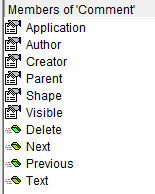
\includegraphics{ExcelMacro/commentobj.png}
 \end{figure}
 
Desde \texttt{Application} hasta \texttt{Visible} son los atributos y desde \texttt{Delete} hasta \texttt{Text} se tienen los métodos.

Si hay un comentario en la celda \textit{F6}, el objeto \texttt{Range("F6")} tiene como atributo \texttt{Comment} (\texttt{range("F6").Comment}) 

\begin{figure}[H]
    \centering
    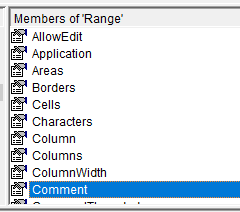
\includegraphics{ExcelMacro/rangeatr.png}
\end{figure}

Por tanto, el objeto \texttt{Comment} tendrá como atributo \texttt{Parent} esa celda:


\begin{verbatim}
?activesheet.Comments(1).Parent.Address
$F$6
\end{verbatim}

\subsubsection{Resumen y conclusiones}

\begin{enumerate}
    \item Para referenciar un objeto se hace a través de su posición en la jerarquía del objeto. El objeto activo es el objeto que está referenciado actualmente; si uno no especifica el objeto padre de una referencia, Excel asumirá que se trata del objeto activo.
    \item No es necesario seleccionar un objeto para manipularlo; aunque existe el método \texttt{Select}, en la práctica no se usa y es más eficiente evitar su uso (aunque hay algunas excepciones) 
\end{enumerate}


\subsection{Referencias a rangos, hojas y libros de Excel con VBA}

El objeto \texttt{Range} es uno de los más importantes y usados en los macros, por lo tanto es importante entender bien y saber cuáles son los métodos y atributos más usados. También cómo se pueden referenciar de forma correcta las diferentes hojas o libros de excel. 

\subsubsection{Métodos de escritura en celdas}

\paragraph{Recordatorio} Diferencia entre los atributos \texttt{Activecell} y \texttt{Selection}, cuando se tiene seleccionadas las celdas \textit{M7:M14}
    \begin{verbatim}
    ?activecell.Address
    $M$7
    ?selection.Address
    $M$7:$M$14
    $K$5
    \end{verbatim}

La siguiente lista muestra cómo referenciar un rango de distintas formas.

\begin{itemize}
    \item \texttt{Range().Value = "1st"} 
    \item \texttt{Range(R1,R2).Value = "hola"} Pone el valor en todas las celdas desde R1 hasta R2. 
    \item \texttt{Range("R1;R2").Value = "hola"} Pone el valor solo en las referencias especificadas R1 y R2
    \item \texttt{Activecell.Value="Otrooo"} Valor en la celda actualmente activa
    \item \texttt{Range("A" \& 6, "J" \& 27) = "6th"} Utiliza índice numérico que puede ser iterado en bucles. Escribe "6th" en las celdas desde A6 hasta J27.
    \item \texttt{Range(Cells(1, 6), Cells(10, 20)) = "6th"} Para referenciar numéricamente un rango y pueda ser implementado en bucles o iteraciones.
    \item \texttt{Range("A1").Offset(7,2).Value = ...} Se ubica en A1 y busca a partir de ahí el movimiento (7,2) para ubicar el valor en esa casilla. 
    \item \texttt{Range("Reference").Value = "Puting here a reference"} Si se le cambia el nombre a una celda como indica la imagen de abajo, se puede referenciar con ese nombre.
    \item \texttt{Rows("12:14").RowHeight = 35} cambia el tamaño de las filas 12 hasta 14.
    \item \texttt{Columns("W:AA").ColumnWidth = 5} cambia el tamaño de las columnas W hasta AA.
    \item \texttt{Range(Columns(7), Columns(10)).ColumnWidth = 5} Tamaño de las columnas desde la 7ma  columna hasta la 10ma usando Range.
    \item \texttt{Range(Rows(7), Rows(10)).RowHeight = 25} Tamaño de las filas desde la 7ma  columna hasta la 10ma usando Range.
    \item \texttt{Cells.Columns.AutoFit} pone tamaño minimo de todas las columnas
\end{itemize}


\begin{figure}[H]
    \centering
    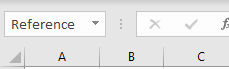
\includegraphics{ExcelMacro/reference.png}
\end{figure}

\subsection{Métodos y atributos más usados e importantes del objeto Range}

Los atributos y métodos más útiles que son necesarios saber y tener en cuenta cómo se trabajan en VBA.

\begin{table}[H]
    \centering
    \begin{tabular}{|m{0.15\columnwidth}|m{0.60\columnwidth}|m{0.1\columnwidth}|}
        \hline
        \rowcolor{lightgray} \textbf{Atributo} & \textbf{Descripción} & \textbf{Tipo} \\ \hline \hline
        \texttt{Value}        & Valor que está escrito en la celda. Es la propiedad por defecto & Lect/Esc \\ \hline
        \texttt{Cells}        & Retorna una celda o un rango de celdas dentro del rango  & Lect/Esc  \\ \hline
        \texttt{End}          & Retorna la última celda del rango. Similar a Ctrl + up, down, left o right. Recibe como argumento una de las cuatro direcciones: \texttt{xlDown, xlToLeft, xlToRight, xlUp} & Solo Lect  \\ \hline
        \texttt{Offset}       & Retorna la celda que está referenciada desde el lugar de origen, cierto número de filas o columnas.  & Lect/Esc  \\ \hline
        \texttt{Count}        & Retorna el número de celdas que hay en el rango  & Solo Lect  \\ \hline
        \texttt{Column/Row}   & Retorna el índice de la fila o columna del rango. Si el rango es de más de una celda, rel retorno es el primero de ellos.  & Solo Lect  \\ \hline
        \texttt{CurrentRegion}& Retorna las celdas o rango que pertenecen a una región de datos.  & Solo Lect  \\ \hline
        \texttt{EntireColumn}/
        \texttt{EntireRow}    & Retorna el rango con todas las celdas de la columna o fila  & Solo Lect \\ \hline
        \texttt{Resize}       & Cambia el tamaño del rango definiendo las filas y columnas para reescalado  & Solo Lect  \\ \hline
        \texttt{Address}      & Retorna la dirección de la celda  & Solo Lect  \\ \hline
        \texttt{Font}         & Retorna el objeto Fuente perteneciente a la celda  & Lect/Esc  \\ \hline
        \texttt{interior}     & Es el relleno o interior de la celda. Tiene sus propios atributos como color y demás  & Lect/Esc  \\ \hline
        \texttt{Formula}      & Escribe una fórmula en la celda(s)   & Lect/Esc  \\ \hline
        \texttt{NumberFormat} & Define el formato numérico de la(s) celda(s)   & Lect/Esc  \\ \hline
        \texttt{Text}         & Retorna el dato que haya en la celda como un string   & Solo Lect  \\ \hline
        \texttt{HasFormula}   & Retorna un valor de verdad o \texttt{Null} si son varias celdas y tiene ambos valores de verdad   & Solo Lect  \\ \hline
    \end{tabular}
    \caption{Diferentes atributos útiles}
    \label{tab_rangea}
\end{table}



\begin{table}[H]
    \centering
    \begin{tabular}{|m{0.15\columnwidth}|m{0.60\columnwidth}|}
        \hline
        \rowcolor{lightgray} \textbf{Método} & \textbf{Descripción} \\ \hline \hline
        \texttt{Copy}         & Es práctico porque tiene su destino como argumento, permitiendo copiar y pegar en una sola línea \\ \hline
        \texttt{PasteSpecial} & Permite las opciones de excel de pegado especial. Para usar más de una opción se repite la línea de código con las nuevas opciones \\ \hline
        \texttt{Clear}        & Borra el contenido y el formato de las celdas  \\ \hline
        \texttt{Delete}       & Borra las celdas y realiza in corrimiento de las celdas adyacentes. Es necesario poner argumentos para el corrimiento de la información   \\ \hline
        \texttt{SpecialCells} & Retorna un rango que coincida con los tipos de celda especificado \\ \hline
        \texttt{Sort}         & Ordena un rango de valores.   \\ \hline
        \texttt{PrintOut}     & Se puede usar para imprimir una hoja. \\ \hline
        \texttt{Select}       & Se usa para seleccionar una celda o un rango de celdas. No es necesario usarlo cuando se hace código en VBA, porque no es necesario seleccionar una celda para manipularla.  \\ \hline
    \end{tabular}
    \caption{Diferentes métodos útiles}
    \label{tab_rangem}
\end{table}

\paragraph{Nota} Puede ser útil, para seleccionar o referenciar la última celda de un rango, si en el rango hay bahías, seleccionar desde abajo, siempre y cuando se tenga cereza que no hay ningún valor más abajo, de la siguiente forma

\begin{verbatim}
Range("K6").Value = Range("A" & Rows.Count).End(xlUp).Row
\end{verbatim}

Con \texttt{"A" \& Rows.Count} se está referenciando la última celda de la columna A.

\subsubsection{Copia y pegado de rangos}


\begin{verbatim}
Sub CopyPaste()
    '--------------
    'Mediante el metodo Copy
    '--------------
    Range("A5").CurrentRegion.Copy Range("J4")
    
    '--------------
    'Mediante el metodo PasteSpecial
    '--------------
    Range("A5").CurrentRegion.Copy
    Range("j20").PasteSpecial xlPasteValues
    Range("j20").PasteSpecial xlPasteComments

    '--------------
    'Mediante el propiedad Resize, para copiar contenido sin header
    '--------------
    Range("A5").CurrentRegion.Offset(1, 0).Resize(Range("A5").CurrentRegion.Rows.Count - 1).Copy
    Range("A20").PasteSpecial xlPasteFormulasAndNumberFormats
    Application.DataEntryMode = False
End Sub
\end{verbatim}

\subsubsection{Referenciando Hojas de excel}

Para que uno pueda referenciar la hoja activa mediante el Intellisense, es necesario declarar la hoja como variable

\begin{verbatim}
Dim Sh As Worksheet
Set Sh = ActiveSheet
\end{verbatim}

De este modo se puede usar el Intellisense con el ctrl + espacio. \\

Las hojas de un libro de excel pueden ser referenciadas con su índice (que empieza por 1).

\begin{verbatim}
Worksheets(6).Select
Sheets(6).Select
Worksheets("Purpose").Select
\end{verbatim}

Aquí "\texttt{sheets}" también puede hacer referencia a hojas que no sean de cálculo como \texttt{chart sheets}. Evidentemente se puede referenciar con el nombre de la hoja. Otra manera es mediante el nombre código de la hoja, este se puede ver en la imagen a continuación


\begin{figure}[H]
    \centering
    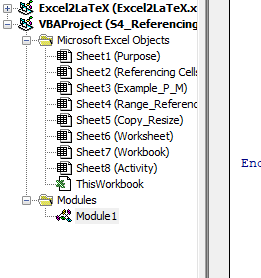
\includegraphics{ExcelMacro/codesheets.png}
\end{figure}

Teniendo en cuenta la imagen, el código sería

\begin{verbatim}
Sheet6.Select
\end{verbatim}

El nombre código de una hoja se puede cambiar.

\subsubsection{Macro que guarda una copia del contenido de un libro}

\begin{verbatim}
ThisWorkbook.Save
Sheets.Select
Cells.Copy
Cells.PasteSpecial xlPasteValues

Application.DisplayAlerts = False

ThisWorkbook.SaveAs Filename:=ThisWorkbook.Path & 
"HC_" & VBA.Format(VBA.Date, "YYMMDD") & "_" & VBA.Replace(ThisWorkbook.Name, ".xlsm", ""),
FileFormat:= Excel.clOpenXMLWorkbook
Application.DisplayAlerts = True

\end{verbatim}

\subsection{Variables y tipos de datos}

Declaración de asignación:
\begin{verbatim}
Range("A1").Value = Date
Range("A1").Value = Range("A1").Value + 1
\end{verbatim}

Para declarar una variable

\begin{verbatim}
myTitle = Range("a8").Value
\end{verbatim}

Los tipos de datos se muestran en la siguiente tabla

\begin{table}[H]
    \centering
    \begin{tabular}{lll}
    \hline
        \textbf{Tipo} & \textbf{Uso de memoria} & \textbf{Rango} \\ \hline
        \rowcolor{micolor1} Byte & 1 byte & 1 a 255 \\ 
        \rowcolor{micolor2} Integer  & 2 bytes & -32768 a 32768 \\
        \rowcolor{micolor1} Long     & 4 bytes & -2147483648 a 2147483648 \\
        \rowcolor{micolor2} Boolean  & 2 bytes & True / False \\
        \rowcolor{micolor1} Double   & 8 bytes & Rango muy grande positivo o negativo con alta precisión \\
        \rowcolor{micolor2} String   & 1 byte por caracter & Depende de la longitud \\
        \rowcolor{micolor1} Object   & 4 bytes & Cualquier objeto \\
        \rowcolor{micolor2} Date     & 8 bytes & 01/01/0100 hasta 12/31/9999 \\
        \rowcolor{micolor1} Currency & 8 bytes & Rango muy grande positivo o negativo hasta 4 decimales \\
        \rowcolor{micolor2} Variant  & 16 bytes o más & Cualquiera, puede ser Vacío, Nada, o Null \\ 
    \end{tabular}
\end{table}

La palabra reservada para declaración de variables es \texttt{Dim}. Una nota importante es que si no se usa la palabra reservada
\texttt{As}, entonces se interpretará el tipo de objeto como \texttt{Variant}.

\begin{verbatim}
Dim myText As String
\end{verbatim}


\paragraph{Nota} se puede usar la palabra reservada \texttt{Debug.Print} para imprimir en consola la variable que se necesite.

\subsubsection{Arrelgos}

Los arreglos (\texttt{Array}) son grupos de variables los cuales tienen el mismo nombre asociado.


Declaración de arreglos

\begin{verbatim}
Dim MyMonth(1 To 12) As String
MyMonth(1) = "Jan"
.
.
.
\end{verbatim}

Si se declara un arreglo de la siguiente forma \texttt{Dim MyMonth(11) As String} se asume el primer índice del arreglo como cero.

Areglos de dos dimensiones:

\begin{verbatim}
Dim MonthSales(1 To 12, 1 To 3) As Variant
Dim MonthSales() As Variant
\end{verbatim}

La última declaración, en la que no hay números en los paréntesis, es un arreglo con tamaño variable.

Para declaración de constantes

\begin{verbatim}
Const MYSCCENARIO As String = "Actual"
\end{verbatim}


Ejempplo de declaración de variables del tipo Objetos


\begin{verbatim}
Dim NewBook As Workbook
Dim NewSheet As Worksheet
Dim NewRange As Range

Set NewBook = Workbooks.Add
\end{verbatim}

\subsubsection{\texttt{scope}}

El scope es es el entorno o subentorno en el que las variables existen, puede ser un sub procedimiento o en todos los sub procedimientos. Las variables solamente existen cuando el procedimiento se está ejecutando. El entorno más pequeño es el entorno de procedimiento. La memoria se libera una vez el procedimiento termina. Un entorno mayor permite declaración de variables que están disponibles en el módulo entero En este caso el \texttt{Dim} está por fuera de cualquier \texttt{Sub}. El valor almacenado permanece en la memoria después de que se ejecuten los procedimientos.

El entorno mayor es aquel en el que se pueden declarar variables para todos los módulos y procedimientos. La palabra reservada para declarar estas variables globales es la siguiente

\begin{verbatim}
Option Explicit
Public LastRow As Long, FirstRow As Long
\end{verbatim}


\subsection{Bucles y ciclos}

\subsubsection{Colecciones}

Las colecciones son conjuntos ordenados de objetos, y pueden ser referenciados como una sola unidad. 

\subsubsection{Secuencia \texttt{With}}

Se usa para hacer un uso más sencillo de código, escribir código más rápido, y para un mantenimiento más fácil. Adicionalmente el código se ejecuta de forma más rápida.

Veamos el siguiente ejemplo

\begin{verbatim}
Set myRange = Range("A10","A" & Cells(Rows.Count, 1).End(xlUp).Row)
myRange.Font.Name = "Arial"
myRange.Font.Size = 12
myRange.Font.Bold = True
\end{verbatim}

Con el adjuntador podemos convertirlo a 

\begin{verbatim}
Set myRange = Range("A10","A" & Cells(Rows.Count, 1).End(xlUp).Row)
With myRange.Font
    .Name = "Arial"
    .Size = 12
    .Bold = True
End With
\end{verbatim}

\subsubsection{Bucle \texttt{For...Each}}


Realiza un iteración del tipo que se escoja dentro de una colección

\begin{verbatim}
Dim Cell As Range
For Each Cell In ActiveSheet.UsedRange
    'Instructions
Next Cell
\end{verbatim}

El siguiente ejemplo es para proteger cada una de las hojas de nuestro cuaderno de excel:

\begin{verbatim}

Sub Protect_All_Sheets()
    Dim Sh As Worksheet
    For Each Sh In ThisWorkbook.Worksheets
        Sh.Protect Password:= "prueba", AllowFormattingCells:= True
        Debug.Print Sh.Name
    Next Sh
    
End Sub

Sub Unprotect_All_Sheets()
    Dim Sh As Worksheet
    For Each Sh In ThisWorkbook.Worksheets
        Sh.Unprotect
        Debug.Print Sh.Name
    Next Sh
    
End Sub
\end{verbatim}

El método \texttt{Protect} tiene varios argumentos, entre los que están \texttt{Password:= "prueba", AllowFormattingCells:= True}, poniendo una contraseña y permitiendo que se cambie el formato de las celdas.

Una forma de proteger el macro con código es mediante \texttt{tools, VBAProject Properties, Protection}.

\subsubsection{\texttt{If...Then}}

El condicional if de toda la vida, es similar a la fórmula de excel y se construye de la siguiente manera

\begin{verbatim}
Sub Simple_if()
    If Range("B3").Value <> "" Then Tange("C3").Value = Range("B3").Value
End Sub    
\end{verbatim}

Con el comparador \texttt{<> ""} se evalúa si la celda en cuestión no está vacía, es decir, si tiene contenido.

\begin{verbatim}
Sub Simple_if()
    If Range("B3").Value <> "" Then 
        Range("C3").Value = Range("B3").Value
    End If
End Sub    
\end{verbatim}

Estructura general de If Else

\begin{verbatim}
If <Comparision> Then
    <Code>
    <Code>
    <Code>
Elseif <Comparision> Then
    <Code>
    <Code>
    <Code>
Else
    <Code>
    <Code>
    <Code>
End If
\end{verbatim}


\subsubsection{\textbf{Case}}

La estructura principal es

\begin{verbatim}
Sub CaseStat()
    Select Case Range("B3").Value
    Case 1 To 200
        Range("c3").Value = "Good"
    Case 0
        Range("c3").Value = "Empty"
    Case Is > 200
        Range("c3").Value = "Excellent"
    Case Else
        Range("c3").Value = "Bad"
End Sub
\end{verbatim}

Se puede seleccionar valores especificos de la siguiente forma

\begin{verbatim}
Case 1,3,7
\end{verbatim}

\subsubsection{\textbf{GoTo}}

Es la declaración para saltar algunas líneas de código o ambiar el flujo del código. La sección a la cual se salta debe ser etiquetada con un identificador.

\begin{verbatim}
Sub SimpleGoTo()
    Range("d3").Value = ""
    If IsError(Range("d3")) Then GoTo GetOut
    Range("c3").Value = Range("b3").Value
    Exit Sub
    
GetOut:
    Range("d3").Value = "u have an error in cell"
End Sub

\end{verbatim}

\subsubsection{Forma de esconder y mostrar hojas de excel con macro}


\begin{verbatim}
Sub Unhide_All()
    Dim sh As Worksheet
    For Each sh In ThisWorkbook.Worksheets
    sh.Visible = True
    Next sh
    
End Sub
\end{verbatim}

Hay una forma para asignar la macro a cualquier archivo de excel sin importar si tiene habilitadas las macros o no. Ver lección 48 de curso.

\subsubsection{Funciones útiles de VBA}

Hay algunas funciones que tienen los objetos \texttt{VBA} y \texttt{excel.WorkSheetFunction} que pueden ser útiles

\begin{table}[H]
    \centering
    \begin{tabular}{c|c}
       \rowcolor{micolor1} Excel & VBA \\ \hline
        \texttt{ ABS() } & \texttt{ Abs } \\
        \texttt{ ISBLANK() } & \texttt{ ISEMPTY } \\
        \texttt{ LEN() } & \texttt{ LEN } \\
        \texttt{ LOWER() } & \texttt{ LCASE }\\
        \texttt{ RAND() } & \texttt{ RND } \\
        \texttt{ TODAY() } & \texttt{ DATE } \\
        \texttt{ TYPE() } & \texttt{ TYPENAME } \\
        \texttt{ UPPER() } & \texttt{ UCASE } \\
    \end{tabular}
\end{table}

\paragraph{Ejemplo} algunas funciones desde \texttt{VBA} y \texttt{Excel}:

\begin{verbatim}
Sub VBA_Excel_Func()
    With ShVEF
        .Range("B3").Value = Date
        .Range("B6").Value = VBA.UCase(.Range("A6").Value)
        .Range("B7").Value = VBA.LCase(.Range("A7").Value)
        .Range("B8").Value = VBA.StrConv(.Range("A8").Value, vbProperCase)
        .Range("B9").Value = Excel.Application.WorksheetFunction.Proper(.Range("A9").Value)
        .Range("B11").Value = 
        Excel.Application.WorksheetFunction.Max(.Range("a13", "c20").Value)
    End With
End Sub
\end{verbatim}

\begin{table}[H]
    \centering
    \begin{tabular}{c|l}
       \rowcolor{micolor1} Manejo de fechas & Descripción \\ \hline
        \texttt{ Date } & Retorna la fecha actual\\
       \texttt{ Day } & Retorna el día del mes de una fecha \\
       \texttt{ Hour } & Retorna la hora de una variable de tiempo \\
       \texttt{ IsDate } & Retorna valor de verdad si es variable fecha \\
       \texttt{ Minute } & Retorna el minuto de una variable de tiempo \\
       \texttt{ Month } & Retorna el mes de una fecha\\
       \texttt{ MonthName } & Retorna un string para el mes de una fecha\\
       \texttt{ Now } & Retorna la fecha y hora actual \\
       \texttt{ Second } & Retorna el segundo de una variable tiempño \\
       \texttt{ Time } & Retorna el tiempo actual del sistema \\
       \texttt{ Timer } & Retorna el numero de segundos que ha transcurrido desde media noche \\
       \texttt{ Weekday } & Retorna el número para el día de la semana\\
       \texttt{ WeekdayName } & Retorna un string para el día de la semana\\
       \texttt{ Yeat } & Retorna el año de una fecha\\
    \end{tabular}
\end{table}

\begin{table}[H]
    \centering
    \begin{tabular}{c|l}
       \rowcolor{micolor1} Formato y conversión & Descripción  \\ \hline
        \texttt{ CDate} & Convierte la expresión a fecha  \\
       \texttt{ CInt } & Convierte la expresión a entero \\
       \texttt{ CLng } & Convierte la expresión a Long \\
       \texttt{ CStr } & Convierte la expresión a string \\
       \texttt{ Format } & Muestra una expresión en el formato deseado \\
       \texttt{ Str } & Retorna un string de un número \\
       \texttt{ Val } &  Retorna el número (double) de un string\\
       \rowcolor{micolor1} Manejo de número & Retorna la fecha y hora actual \\
       \texttt{ Abs } & Valor absoluto \\
       \texttt{ FormatNUmber } & Formatea la expresión como número \\
       \texttt{ FormatPercent } & Da formato de porcentaje \\
       \texttt{ IsNumeric } & Valor de verad de si es numero\\
       \texttt{ Round } & redondea\\
    \end{tabular}
\end{table}

\begin{table}[H]
    \centering
    \begin{tabular}{c|c}
       \rowcolor{micolor1} Directorios y textos & Descripción \\ \hline
       \texttt{ CurDir } & Retorna la ruta actual\\
       \texttt{ Dir } & Retorna el nombre del a rchivo o directorio \\
       \texttt{ EOF } & Si se alcanza el final del archivo de texto, se iguala a verdadero \\
       \texttt{ FileDateTime } & Fecha y hora de la última modificación de un archivo\\
       \texttt{ FileLen } & Número de bytes en un archivo\\
       \texttt{ FreeFile } & Retorna el siguiente número de archivo disponible para archivos de texto  \\
       \rowcolor{micolor1} Otras & Descripción \\ \hline
       \texttt{ DoEvents } & El control se devuelve al sistema operativo para procesar otros eventos\\
       \texttt{ InputBox } & Muestra una caja de diálogo para que el usuario ingrese datos\\
       \texttt{ IsEmpty } & Retorna si la celda está vacía\\
       \texttt{ LBound } & Retorna el valor más pequeño en un arreglo\\
       \texttt{ MsgBox } & Muestra una caja de diálogo\\
       \texttt{ RGB } & Retorna un número que refleja el color RGB \\
       \texttt{ TypeName } & Retorna un string que especifica el tipo de dato de una variable\\
       \texttt{ Ubound } & retorna el elemento más grande de un arreglo \\
    \end{tabular}
\end{table}

\subsubsection{Cuadros de diálogo}

El cuadro de diálogo más básico que solamente muestra un mensaje es el siguiente:

\begin{verbatim}
Sub activity()
    'VBA.Interaction.MsgBox
    VBA.MsgBox ("Hello")
End Sub
\end{verbatim}

El siguiente procedimiento muestra un cuadro de diálogo en el que el usuario debe responder con "sí" o "no" y la macro guarda esta decisión para realizar algo

\begin{verbatim}
Sub act2()
    Dim answer As VbMsgBoxResult
    answer = VBA.MsgBox("Seguro de querer borrar?", vbYesNo + vbQuestion, "Clear Cells")
    If answer = vbYes Then
        Range("A7:B9").Clear
    Else
        Exit Sub
        End If
End Sub
\end{verbatim}

El argumento \texttt{vbQuestion} solo sirve para poner el icono de interrogante en el cuadro de diálogo, note cómo con el signo "+" se añaden más argumentos.

\subsubsection{Cuadros de diálogo con entrada de datos}

Para que el usuario pueda introducir datos utilizables por el programa, se usa la función \texttt{Inputbox}. El retorno de esta función \textbf{siempre será un string}. Si el usuario escribe el resultado de la entrada a una celda, Excel convertirá automáticamente la respuesta al tipo correcto. por ejemplo, si se ingresa un número y este se escribe en una celda, este será reconocido automáticamente como un número.

Si la respuest aes requerida dentro del código, y esta debe ser un número, es ecesario convertir el dato a entero o a double. Se puede usar la función \texttt{Val}, y se puede usar también la función \texttt{IsNumeric} para validar. 

El siguiente ejemplo es un código que pregunta al usuario por una entrada cualquiera y la pone al final de una lista.

\begin{verbatim}
Sub VBA_InputBox_Task2()
    Dim myImp As String
    myImp = InputBox("Please input the next string","Here below")
    range("A5").end(xldown).offset(1,0).value = myImp
End Sub
\end{verbatim}

\subsubsection{Método de cuadro de diálogo con entrada de datos con Excel}

Los beneficios que se obtienen con este método son:

\begin{enumerate}
    \item Se puede especificar el tipo de dato que se va a ingresar. No está restringido solamente a string.
    \item Excel realiza una validación del tipo de dato de manera automática.
    \item Se pueden seleccionar rangos.
\end{enumerate}

El siguiente código es una cuadro de dialogo que ingresa un nombre de cliente y un número para agregarlos al final de una tabla.

\begin{verbatim}
Sub Excel_inputBxTask1()
    Dim Cname As String
    Dim NextRow As Long
    Dim CAmount As Long
    Cname = VBA.InputBox("Please enter new customer name", "Customer Master")
    NextRow = Cells(Rows.Count, 1).End(xlUp).Row + 1
    Cells(NextRow, 1).Value = Cname
    CAmount = Excel.Application.InputBox(Prompt:="Please enter Amount", Title:="Entering Amount", Type:=1)
    Cells(NextRow, 2).Value = CAmount
End Sub
\end{verbatim}

Es importante notar que uno de los argumentos de la función \texttt{Excel.Application.InputBox} es \texttt{Type}, este indica el tipo de dato que será ingresado en el cuadro, si se ingresa un dato no correspondiente, saltará un error y deberá ingresar nuevamente. La siguiente tabl muestra los diferentes códigos para los tipos de datos que se pueden ingresar con la función.

\begin{table}[H]
    \centering
    \begin{tabular}{l|l}
        \rowcolor{micolor1} Código & Descropción \\ \hline
        0 & Fórmula \\
        1 & Número \\
        2 & String \\
        4 & Boolean \\
        8 & Range \\
        16 & Error Value \\
        64 & Array of values \\
        1+2=3 & Number + String \\
    \end{tabular}
\end{table}


 El código siguiente es un ejemplo de ingreso de un rango de excel y se cuenta el número de celdas vacías, con múmeros y de otros tipos.
 
 
\begin{verbatim}
Sub Excel_inputBxTask2()
    Dim myRange As Range
    Dim cellblank As Long, cellNum As Long, cellOther As Long
    
    Set myRange = Excel.Application.InputBox(Prompt:="Please Select the range", Title:="Range", Type:=8)
    cellblank = Excel.WorksheetFunction.CountBlank(myRange)
    cellNum = Excel.WorksheetFunction.Count(myRange)
    cellOther = Excel.WorksheetFunction.CountA(myRange) - cellNum
    MsgBox cellblank & " celdas están en blanco" & vbNewLine & cellNum & " celdas contienen números" & vbNewLine & cellOther & " son no numericas"
End Sub
\end{verbatim}

Si durante la captura de dato a ingresar se le da cancelar, el programa arroja un error, porque el programa espera siempre el tipo de dato. Para manejar este error se usa el siguiente código

\begin{verbatim}
Sub Excel_inputBxTask2()
    Dim myRange As Range
    Dim cellblank As Long, cellNum As Long, cellOther As Long
    
    Set myRange = Excel.Application.InputBox(Prompt:="Please Select the range", Title:="Range", Type:=8)
    On Error GoTo Leave
    cellblank = Excel.WorksheetFunction.CountBlank(myRange)
    cellNum = Excel.WorksheetFunction.Count(myRange)
    cellOther = Excel.WorksheetFunction.CountA(myRange) - cellNum
    MsgBox cellblank & " celdas están en blanco" & vbNewLine & cellNum & " celdas contienen números" & vbNewLine & cellOther & " son no numericas"
Leave:
End Sub
\end{verbatim}

Mediante la sentencia \texttt{GoTo}.


\subsubsection{Ejercicios}

El primer ejercicio consiste en crear una macro que permita al usuario seleccionar un rango, una vez se seleccione, aparezca una caja de diálogo que muestre los tres valores más grandes del rango.

\section{Depuración y manejo de errores}


Las opciones principales o más importantes para realizar depuración del código son las siguientes:

\begin{enumerate}
    \item Con \texttt{F8} o seleccionando\texttt{Debug} en el menú y luego \texttt{Step Into}.
    \item Añadiendo puntos de quiebre con \texttt{F9} para analizar el comportamiento del codigo en este o estos puntos. A partir de ahí se puede ir paso por paso con \texttt{F8}
    \item Pasando el cursor encima de las variables y de esta forma ver el valor que tiene la misma.
    \item El uso de la "Immediate Window". Con la palabra reservada \texttt{Debug.Print} seguido de la variable, se imprime en esta ventana el valor de la variable. También se puede escribir directamente en la ventana con el comando reservado \texttt{?} para conocer el valor de cualquier variable u objeto
    \item Usando la ventana de locales (se activa en el menú "ver") para ver los valores y las características asociadas a cada variable.
    \item Con la \textbf{Ventana de Vista (Watch Window)} para mantener monitorizadas ciertas variables. Con el click derecho sobre una variable y la opción "add to watch". O arrastrarla ala misma ventana. Se pueden cambiar directamente las propiedades de la variable escribiendo directamente en ella. 
\end{enumerate}


\subsection{Manejo de errores}

Los siguientes son ejemplos sencillos para el manejo de posibles errores durante la ejecución del código:

\begin{verbatim}
Sub Jump_to_End()
    On Error GoTo Leave
    
    <Code>
    .
    .
    .
    
Leave:
EndSub
\end{verbatim}



Con el \texttt{GoTo} se permite saltar el conjunto de instrucciones para terminar el código en caso de que salte un error. La desventaja de este método es que no hay forma de obtener información en caso de que se salte algún error que no esté previsto.



\begin{verbatim}
Sub Resume_Then_Normal()
    On Error Resume Next
    
    <Code>
    .
    .
    .
    
    On Error Goto 0
    
    <Code>
    .
    .
    .
End Sub
\end{verbatim}


Este código ignora la línea que está produciendo el error y continúa ejecutando la siguiente línea.


\begin{verbatim}
Sub Handle_Based_onError_Type()
    On Error GoTo ErrorHandle
    
    <Code>
    .
    .
    .
    
    Exit Sub
    
ErrorHandle:
    Select Case Err.Number
        Case 424
            Exit Sub
        Case Else
            MsgBox "An Error has occurred."
    End Select
End Sub
\end{verbatim}


Esta tercera opción verifica cuál es el tipo de error que saltó, y realiza el procedimiento que se le asigne en consecuencia.

\subsection{Optimización de la ejecución}

Cuando se tiene un código muyy extenso, este puede demorar en ejecutarse. Existen formas de mejorar el desempeño del código

\paragraph{Ejemplo}

\begin{verbatim}
Sub Slower_Code()
    Dim ShNew As Worksheet
    Dim cell As Range
    
    Set ShNew = Worksheets.Add
    
    For Each cell In ShNew.Range("A1:A100000")
        cell.Value = cell.Row
    Next cell
End Sub
\end{verbatim}

Esta macro podría demorar bastante en ejecutarse, porque trabaja con muchas celdas. Por lo tanto una forma buena de disminuir el tiempo de ejecución es mediante los siguientes comandos


\begin{verbatim}
With Application
    .StatusBar = "Wait..."
    .ScreenUpdating = False
    .DisplayAlerts = False
    .Calculation = xlCalculationManual
End With
\end{verbatim}

Evidentemente es necesario volver a configurar estos parámetros a sus valores originales 


\begin{verbatim}
With Application
    .StatusBar = ""
    .ScreenUpdating = True
    .DisplayAlerts = True
    .Calculation = xlCalculationAutomatic
End With
\end{verbatim}


Es importante identificar los códigos de errores para tener un sistema eficiente de manejo de los mismos.



\subsection{Procedure scope}

Una pregunta importante acerca de los subprocedimientos es cómo se puede saber si son locales o globales o privados, desde dónde en el código se tiene acceso a un subprocedimiento en particular. \\

Por defecto los subprocedimientos son públicos. Los procedimientos privados solamente están disponibles desde otros que estén en el mismo módulo. Por lo tanto no se verán en la lista de macros y no podrán ser asignados a un botón. \\

Para llamar a un procedimiento desde el interior de otro se usa la palabra reservada \texttt{Call}

\begin{verbatim}
Sub ejemploCall()
    Call Faster_Code
End Sub
\end{verbatim}

\subsection{Argumentos en los sub-procedimientos}

El siguiente ejemplo ilustra los argumentos para los subprocedimientos.

\begin{verbatim}
 
Private Sub muCalc(GetValue As Double, myPercent)
    GetValue = GetValue * myPercent
    MsgBox GetValue
End Sub


Sub GetMyValue()
    Dim myvalue As Double
    Dim p As Variant
    myvalue = Range("A8").value
    p = Range("B8").value
    Call muCalc(myvalue, p)
End Sub
\end{verbatim}

Como nota adicional, si en el argumento del procedimiento ponemos la palabra reservada \texttt{ByRef}, es decir 

\begin{verbatim}
Private Sub muCalc(ByRef GetValue As Double, myPercent)
    GetValue = GetValue * myPercent
    MsgBox GetValue
End Sub
\end{verbatim}


Estamos asignando como argumento la variable en í, es decir, si cambiamos el valor de la misma en el subprocedimiento, este se verá cambiado también en el subprocedimiento que lo llamó, por otro lado, 



\begin{verbatim}
Private Sub muCalc(ByVal GetValue As Double, myPercent)
    GetValue = GetValue * myPercent
    MsgBox GetValue
End Sub
\end{verbatim}

Sirve para pasar una copia del valor de la variable como argumento, para que no sea cambiada en caso de que así se requiera.

\subsection{Ejemplo de macro}

El siguiente ejemplo es un mini-proyecto que sirve para obtener el número total de fórmulas y comentarios en un libro de trabajo.

En primer lugar se debe tener en cuenta que el programa recorre todas las hojas del lobro de trabajo, por lo que es necesario construir un \texttt{for}, y antes, una variable del tipo \texttt{worksheet}. Recordar que con \texttt{For Each Sh In ThisWorkbook.Worksheets} se puede recorrer cada hoja dentro del workbook activo. \\

El código queda como sigue

\begin{verbatim}
Sub countFormulas()
    Dim Sh As Worksheet
    Dim counterWS As Integer
    For Each Sh In ThisWorkbook.Worksheets
        On Error GoTo ErrorHandle
        counterWS = Sh.Cells.SpecialCells(xlCellTypeFormulas).Count
ShowMsg:
        MsgBox ("The sheet " & Sh.Name & " has " & counterWS & " Formulas")
ErrorHandle:
        If Err.Number = 1004 Then
                counterWS = 0
                Resume ShowMsg
        End If
    Next Sh
    
End Sub


Sub countComments()
    Dim Sh As Worksheet
    Dim counterWS As Integer
    For Each Sh In ThisWorkbook.Worksheets
        On Error GoTo ErrorHandle
        counterWS = Sh.Cells.SpecialCells(xlCellTypeComments).Count
ShowMsg:
        MsgBox ("The sheet " & Sh.Name & " has " & counterWS & " Comments")
ErrorHandle:
        If Err.Number = 1004 Then
                counterWS = 0
                Resume ShowMsg
        End If
    Next Sh
    
End Sub
\end{verbatim}


Observe cómo se está manejando el posible error que puede saltar al no encontrar celdasa con el comando \texttt{secialCells}.


\subsection{Resumen}

\section{Proyecto 1: Insertar automáticamente una tabla de contenidos}

La primera parte de este proyecto es añadir en la hoja de contenido los nombres que asignemos a cada una de las demás hojas:

\begin{verbatim}
Sub Auto_Table()
    Dim StartCell As Range
    Dim Sh As Worksheet
    Dim c As Integer
    
    Set StartCell = Excel.Application.InputBox("Insert the range", 
    "Insert Table of Contents", , , , , , 8)
    Set StartCell = StartCell.Cells(1, 1)
    c = 0
    
    For Each Sh In ThisWorkbook.Worksheets
        StartCell.Offset(c, 0).value = Sh.Range("a1").value
        c = c + 1
    Next Sh
End Sub
\end{verbatim}

Luego se añade un hipervínculo para que dirija hacia la hoja necesaria:

\begin{verbatim}
Sub Auto_Table()
    Dim StartCell As Range
    Dim Sh As Worksheet
    Dim ShName As String
    Dim c As Integer
    
    Set StartCell = Excel.Application.InputBox("Insert the range", 
    "Insert Table of Contents", , , , , , 8)
    Set StartCell = StartCell.Cells(1, 1)
    c = 0
    
    For Each Sh In ThisWorkbook.Worksheets
        ShName = Sh.Name
        If ActiveSheet.Name <> ShName Then
            StartCell.Offset(c, 1).value = Sh.Range("a1").value
            ActiveSheet.Hyperlinks.Add anchor:=StartCell.Offset(c, 0), Address:="", 
            SubAddress:=ShName & "!A1", TextToDisplay:=ShName
            c = c + 1
        End If
    Next Sh
End Sub
\end{verbatim}


Importante notar que el argumento \texttt{Anchor} es la celda en la cual se pondrá el hipervínculo, \texttt{SubAddress} es el lugar hacia el cual nos va a dirigir el hipervínculo.\\

Ahora amos a evitar algunos errores, por ejemplo, si se le da a cancelar


\begin{verbatim}
Sub Auto_Table()
    Dim StartCell As Range
    Dim Sh As Worksheet
    Dim ShName As String
    Dim c As Integer
    
    On Error Resume Next
    
    Set StartCell = Excel.Application.InputBox("Insert the range",
    "Insert Table of Contents", , , , , , 8)
    
    If Err.Number = 424 Then Exit Sub
    'on error goto Handle
    
    Set StartCell = StartCell.Cells(1, 1)
    c = 0
    
    For Each Sh In ThisWorkbook.Worksheets
        ShName = Sh.Name
        If ActiveSheet.Name <> ShName Then
            StartCell.Offset(c, 1).value = Sh.Range("a1").value
            ActiveSheet.Hyperlinks.Add anchor:=StartCell.Offset(c, 0), Address:=""
            , SubAddress:=ShName & "!A1", TextToDisplay:=ShName
            c = c + 1
        End If
    Next Sh
    Exit Sub
handle:
    MsgBox "Hubo un error al creal la tabla de contenido."
    
End Sub
\end{verbatim}


\section{Bucles}

En esta sección se habla de manera más detallada sobre diferentes formas de hacer iteraciones y bucles en VBA.

\subsection{For Next}

Se puede denominar como un bucle contador dado que su estructura está basada en un contados específico. Se puede salir del buble en cualquier momento con la sentencia \texttt{exit for}.

\begin{verbatim}
Sub Simple_For()
    Dim i As Long
    Dim MyValue As Double
lastrow = ActiveSheet.usedrangle.Cells(ActiveSheet.usedtange.Rows.Count, 1).Row
For i = 4 To lastrow
    MyValue = Range("f" & i).value
    If MyValue > 400 Then Range ("f" & i), value = MyValue + 10
    If MyValue < 0 Then Exit For
    Next i
End Sub
\end{verbatim}

Se puede seleccionar el método de paso de la iteración de la siguiente manera

\begin{verbatim}
For i = lastrow To 4 Step -1
    <Code>
    <Code>
    <Code>
    <Code>
    Next i
\end{verbatim}


\subsubsection{Ejemplo 1}

En este ejemplo se recorre un rango de una tabla y se separa las letras de los números para ponerlos en otras celdas seleccionadas.

\begin{verbatim}
Sub Simple_For()
    Dim i As Long
    Dim j As Long
    Dim MyValue As String
    Dim LastRow As Long
    Dim NumFound As Long
    Dim TxtFound As String
    Dim FinalValue As Long
    Dim StartValue As Long
    
    'MyValue = Range("a10").Value
    StartValue = Range("a10").Row
    FinalValue = Range("a10").End(xlDown).Row
    
    For j = StartValue To FinalValue
        MyValue = Range("a" & j).Value
        For i = 1 To VBA.Len(MyValue)
            If IsNumeric(VBA.Mid(MyValue, i, 1)) Then
                NumFound = NumFound & VBA.Mid(MyValue, i, 1)
            ElseIf Not IsNumeric(VBA.Mid(MyValue, i, 1)) Then
                TxtFound = TxtFound & VBA.Mid(MyValue, i, 1)
            End If
        Next i
        Range("h" & j).Value = NumFound
        Range("i" & j).Value = TxtFound
        NumFound = 0
        TxtFound = ""
    Next j
    
    End Sub
\end{verbatim}


\subsubsection{Ejemplo 2}

Este siguiente ejemplo muestra un bucle recorrido desde el final. Esta forma es útil cuando, por ejemplo, se necesita eliminar celdas, con lo cual el número de la columna de las celdas inferiores cambia.

\begin{verbatim}
    For i = LastRow To startrow Step -1
        If Rows(i).Hidden = True Then
            Rows(i).Delete
        End If
    Next i
\end{verbatim}

\subsection{Do until y do while}

\texttt{Do Until} puede traducirse como "hacer hasta que... se cumpla


\texttt{Do While}, por su parte, puede traducirse como "hacer mientras que ... se cumpla


Ejemplos:

\begin{verbatim}

Sub Simple_Do_Until()

    Dim StartCell As Integer
    
    StartCell = 8
    Do Until Range("a" & StartCell).Value = ""
        Range("b" & StartCell).Value = Range("a" & StartCell).Value + 10
        StartCell = StartCell + 1
    Loop

End Sub

Sub Simple_Do_While()

    Dim StartCell As Integer
    
    StartCell = 8
    Do While Range("a" & StartCell).Value <> ""
        Range("c" & StartCell).Value = Range("a" & StartCell).Value + 10
        StartCell = StartCell + 1
    Loop

End Sub


Sub Simple_Do()

    Dim StartCell As Integer
    
    StartCell = 8
    Do
        If Range("a" & StartCell).Value = "" Then Exit Do
        Range("d" & StartCell).Value = Range("a" & StartCell).Value + 10
        StartCell = StartCell + 1
    Loop

End Sub
\end{verbatim}

\subsubsection{Ejemplo práctico}

El siguiente es un buen ejemplo de uso del bucle, enb ete ejemplo se pide al usuario escribir un número y si no se ingresa un número, que sedará preguntando siempre.


\begin{verbatim}
Sub Only_Numeric()

    Dim Answer As String
    
    Do While IsNumeric(Answer) = False
        Answer = VBA.InputBox("Please input number")
        If IsNumeric(Answer) Then MsgBox "Bien!"
    Loop
    
End Sub
\end{verbatim}


\subsection{Método Find}


El siguiente programa busca solo un resultado y colorea la celda.

\begin{verbatim}
Sub Buscar_Celda()

    Dim CompID As Range
    Set CompID = Range("A:A").Find(Range("b3"), , xlValues, xlWhole)
    
    'Debug.Print Range("A:A").Find(Range("b3"), , xlValues, xlWhole).Address

    
    With CompID.Interior
        .Pattern = xlSolid
        .PatternColorIndex = xlAutomatic
        .ThemeColor = xlThemeColorAccent2
        .TintAndShade = 0.799981688894314
        .PatternTintAndShade = 0
    End With
End Sub
\end{verbatim}

Cuando la búsqueda no arroja resultados, el rango \texttt{CompID} queda asignado como \texttt{Nothing}, para evitar errores dericados de esto, se puede realizar lo siguiente

\begin{verbatim}
Sub Buscar_Celda()

    Dim CompID As Range
    Set CompID = Range("A:A").Find(Range("b3"), , xlValues, xlWhole)
    
    If Not CompID Is Nothing Then
    
        With CompID.Interior
            .Pattern = xlSolid
            .PatternColorIndex = xlAutomatic
            .ThemeColor = xlThemeColorAccent2
            .TintAndShade = 0.799981688894314
            .PatternTintAndShade = 0
        End With
    Else
        MsgBox "No hay resultados."
    End If
End Sub
\end{verbatim}


Ahora, si tenemos más de un resultado, el siguiente código funcionará:

\begin{verbatim}

    Set CompID = Range("A:A").Find(Range("b3"), , xlValues, xlWhole)
    
    If Not CompID Is Nothing Then
    
       <code>
       <code>
       <code>
       
        FirstMatch = CompID.Address
        
        Do
            Set CompID = Range("A:A").FindNext(CompID)
            If CompID.Address = FirstMatch Then Exit Do
            
                <code>
                <code>
                <code>
        Loop
    Else
        MsgBox "No hay resultados."
    End If
\end{verbatim}

\subsection{Actividad búsqueda de comentarios}

en esta actividad se van a listar los comentarios que hay en todo el libro de excel y se va a guardar en una nueva hoja de trabajo


\begin{verbatim}
Sub actividad()


    Dim sh As Worksheet
    Dim shet As Worksheet
    Dim comentario As Comment
    Dim r As Long 'contador para columnas

'    Pasos para desarrollo de actividad
'   1. Crear una hoja nueva

    Set sh = Worksheets.Add
    

'   2. Poner los titulos para cada item de los comentarios
    With sh
        .Cells(1, 1) = "Comment"
        .Cells(1, 2) = "Address"
        .Cells(1, 3) = "Author"
    
'   3. Poner el contenido de cada comentario en el libro en las celdas
'   4. poner la dirección de cada comentario y la infrmación complementaria

    r = 2
    
    For Each shet In ThisWorkbook.Worksheets
    For Each comentario In shet.Comments
        .Cells(r, 1) = comentario.Text
        .Cells(r, 2) = shet.Name & "! " & comentario.Parent.Address
        .Cells(r, 3) = comentario.Author
        r = r + 1
    Next comentario
    Next shet
    
    .Columns.AutoFit
    End With



End Sub

\end{verbatim}

\subsection{Algunos comandos útiles}

\begin{table}[H]
    \centering
    \begin{tabular}{c|c}
    Nombre     & Descripción \\ \hline \hline
    \texttt{ Const }             & Declara una constante  \\ \hline
    \texttt{ Dim }               & Declara una variable  \\ \hline
    \texttt{ End }               & Se sale de un programa, también finaliza procedimientos, estamentos with, etc. \\ \hline
    \texttt{ Function }          & Declara una función  \\ \hline
    \texttt{ Kill }              & Borra un archivo  \\ \hline
    \texttt{ Let }               & Asigna una variable a una expresión (es opcional, puede ser omitido.  \\ \hline
    \texttt{ Like }              & Retorna Verdadero si un string puede ser emparejado con otro  \\ \hline
    \texttt{ Load }              & Carga un objeto pero no lo muestra  \\ \hline
    \texttt{ Mid }               & reemplaza caracteres en un a cadena por otros caracteres  \\ \hline
    \texttt{ Option Explicit }   & Fuerza una declaracion de variables  \\ \hline
    \texttt{ Public }            & Declara una variable publica  \\ \hline
    \texttt{ ReDim }             & Cambia la dimensión de un arreglo  \\ \hline
    \texttt{ Set }               & Asingna un objeto a una variable  \\ \hline
    \texttt{ Sub }               & declara el nomnbree de un subprocedimiento  \\ \hline
    \texttt{ Call }              & Llama otro dubprocedimiento para ejecutar  \\ \hline
    \end{tabular}
\end{table}

\section{Trabajando con arreglos}
% \chapter{Core games}

\section*{Configuración de ejemplo}

\subsection{Balcony}

Position = 0,0,1200
Rotation = 0,0,0
Scale = 1,1,1

\subsection{Lower area}

Position = 0,0,600
Rotation = 0,0,0
Scale = 1,1,1

\subsection{Basement}

Position = 0,0,0
Rotation = 0,0,0
Scale = 1,1,1

\subsection{Roof}

Position = 0,0,1800
Rotation = 0,0,0
Scale = 1,1,1

\subsection{Decorations}

Position = 0,0,0
Rotation = 0,0,0
Scale = 1,1,1

\subsection{Environment}

Position = 4400,1359,1100
Rotation = -90,0,0
Scale = 1,1,1


\section{Ejemplo rotacion puerta}

\subsection{BasicDoorControllerServer}

\subsubsection{GetDoorRotation()}

Retorna el nivel de rotación de la puerta en valores de [0,1] cuando el angulo es [0,90]

\subsubsection{ SetCurrentRotation(rotation)}

Ajusta

\subsubsection{}

\subsubsection{}

\subsubsection{}

\subsubsection{}

\subsubsection{}

\subsubsection{}

\subsubsection{}

\subsubsection{}

\subsubsection{}

\subsubsection{}

\subsubsection{}

% \chapter{Control}

\section{Conceptos básicos del control clásico}

\subsection{Análisis de error}


En un sistema de realimentación no unitaria podemos considerar el error 

\begin{equation*}
e(t) = r(t) - y(t)
\end{equation*}

en donde la señal de referencia es la señal de salida $y(t)$ está siguiendo, cuando el sistema tiene realimentación unitaria.

El error en estado estavble es

\begin{equation*}
e_{ss} = \lim_{t \to \infty} e(t)
\end{equation*}


\begin{figure}[H]
    \centering
    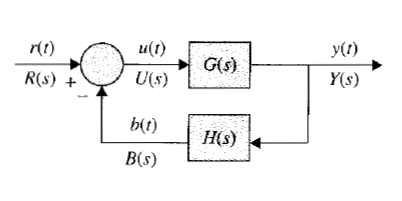
\includegraphics{Control/control_errorf2.png}
\end{figure}

en general si la realimentación es no unitaria, la señal $u(t)$ puede ya no será el error del sistema. Si el propósito del sistema es hacer que la salida siga a la referencia tan cerca como sea posible, y que las funciones de transferencia sean 




\begin{figure}[H]
    \centering
    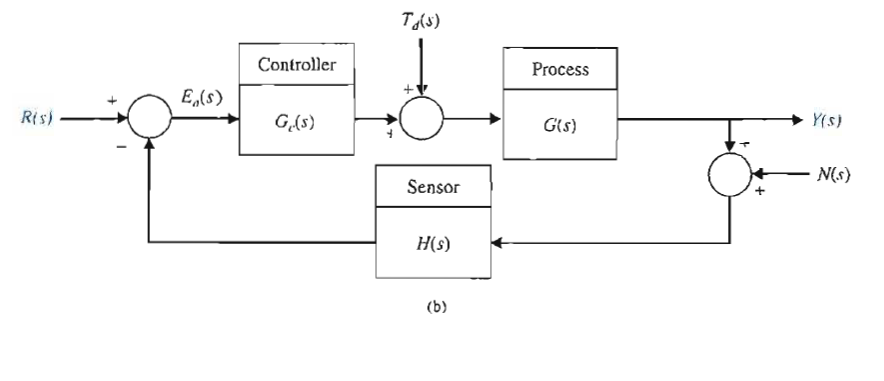
\includegraphics[scale=0.5]{Control/control_errorf1.png}
\end{figure}


El sistema de control de lazo cerrado mostrado en la figura anterior tiene tres entradas $R_(s)$, $T_d(s)$, y $N(s)$ y una salida. Las entradas $T(s)$ y $N(s)$ son señales de perturbaciones y de ruido respectivamente. Se define el error de seguimiento como

\begin{equation*}
E(s) = R(s) - Y(s)
\end{equation*}

Consideremos una realimentación unitaria, esto es $H(s) = 1$. Analizando este sistema de control encontramos que la salida del sistema está dada por

\begin{equation*}
Y(s) = R_(s) \frac{C(s)G(s)}{1 + C(s)G(s)} + T_d(s) \frac{G(s)}{1 + C(s)G(s)} - N(s) \frac{C(s)G(s)}{1 + C(s)G(s)}
\end{equation*}

como $E(s) = R(s) - Y(s)$, tenemos que, restando a $R(s)$ la expresión anterior

\begin{eqnarray*}
E(s) = \frac{1}{1 + C(s)G(s)}R(s) - \frac{G(s)}{1 + C(s)G(s)} T_d(s) + \frac{C(s)G(s)}{1 + C(s)G(s)} N(s)
\end{eqnarray*}

Llamemos a $L(s)=C(s)G(s)$ la función de lazo, esta función es importante en el análisis de sistemas de control. En términos de $L(s)$, la función de error se escribe:

\begin{equation*}
E(s) = \frac{1}{1+L(s)} R(s) - \frac{G(s)}{1+ L(s)}T_d(s) + \frac{L(s)}{1+L(s)}
\end{equation*}

Llamemos ahora a la función $F(s) = 1 + L(s)$ y definamos la función de sensiblildad como

\begin{equation*}
S(s) = \frac{1}{F(s)} = \frac{1}{1+L(s)}
\end{equation*}

y de manera similar definamos la función complementaria de sensibilidad como

\begin{equation*}
C_c(s) = \frac{L(s)}{1+L(s)}
\end{equation*}

Podemos escribir la función de error como

\begin{equation*}
E(s) = S(s) R(s) - S(s) G(s) T_d(S) + C_c(s) N(s)
\end{equation*}

vemos que para poder minimizar el error dada una función de transferencia $G(s)$, necesitamos que las funciones $S(s)$ y $C_c(s)$ sean muy pequeñas. (CONTINUAR LIBRO DORF PAG 215)


\section{Introducción y enfoques del control óptimo robusto}

\subsection{Estabilidad}

Para un sistema no lineal 

\begin{equation*}
    \dot{x} = A(x)
\end{equation*}

Donde $x \in \mathbb{R}^{n}$ y la función $A:\mathbb{R}^{n} \rightarrow \mathbb{R}^{n}$ es no lineal. Si $A(0) = 0$, el punto de equilibrio $x_0=0$ es asintóticamente estable si existe una vecindad de $x_0=0$ tal que si el sistema inicia en la vecindad, entonces su trayectoria converge al punto de equilibrio $x_0=0$ cuando $t \to \infty$.

Si el sistema es no lineal, determinar la estabilidad no es tarea sencilla. Una forma es con el enfoque de Lyapunov; una función de Lyapunov se define a partir de un sistema, esta función puede ser vista como una función de energía para el sistema. Esta función debe tener una propiedad de que su valor es cero en el origen y positiva en los demás lugares. Se asume también que la dinámica del sistema es tal que la energía del sistema es monótonamente decreciente con el tiempo y eventualmente llega a cero. Entonces las trayectorias del sistema no tienen otro lugar al cual dirigirse que no sea el origen. Por lo tanto el sistema es asintóticamente estable. Esta función generalizada de energía se denomina función de Lyapunov. \\

Por otro lado, para un sistema LTI $\dot{x}=Ax$, la estabilidad está dada por su ecuación característica.

\subsection{Control Óptimo}

Luego de estabilizar un sistema, lo siguiente que se quiere es optimizar el desempeño del sistema. Se formula el problema de control óptimo para un sistema general no lineal

\begin{equation*}
    \dot{x} = f(x,u)
\end{equation*}

y se requiere minimizar una función de costo

\begin{equation*}
    J(x,t) = \int_{t}^{t_f} L(x,u) d \tau
\end{equation*}

la función $L(x,u)$ caracteriza el objetivo de costo.\\

La solución del problema de control óptimo se deriva del principio de optimización, el cual establece que si un control es óptimo desde un estado inicial, entonces debe satisfacer la siguiente propiedad: luego de cualquier periodo inicial, el control del sistema para el periodo restante debe ser también óptimo con respecto al estado resultante del control en el periodo inicial. Aplicando el principio de optimización al problema de control óptimo, se puede derivar la ecuación Hamilton-Jacobi-Bellman que debe ser satisfecha por cualquier solución de controlador. \\

No siempre es sencillo resolver la ecuación Hamilton-Jacobi-Bellman, especialmente para sistema no lineales. Sin embargo, si el sistema es lineal y la función de costo es cuadrática, eso es

\begin{equation*}
    \dot{x} = A x + B u
\end{equation*}
\begin{equation*}
    J(x,t) = \int_{t}^{\infty} (x^TQ x+u^{T}R u)d \tau
\end{equation*}

Entonces dicha ecuación complicada se reduce a la siguiente ecuación de Riccati

\begin{equation*}
    S A + A^T S + Q - S B R^{-1} B^{T} S = 0
\end{equation*}

Al resolver la ecuación anterior de Riccati, para $S$, podemos obtener la solución para la señal de control:

\begin{equation*}
    u^{*} = - R^{-1} B^{T} S x
\end{equation*}

El anterior es el problema de control mediante regulador lineal cuadrático (LQR). El problema dual al regulador LQR es el de diseñar un observador óptimo, se denomina filtro de Kalman.

\subsection{Enfoque de control óptimo}

El sistema a ser controlado se describe por la siguiente forma

\begin{equation*}
    \dot{x}A(p)x + B u
\end{equation*}

Donde $p$ representa la incertidumbre. El objetivo es diseñar un estabilizador de realimentación de estados del sistema para todas las incertidumbres posibles $p$. La solución para este problema de control robusto depende de si la incertidumbre satisface una condición de coincidencia, lo cual requiere que la incertidumbre esté dentro de un rango dado por $B$. Si la incertidumbre satisface la condición de coincidencia, entonces la solución al problema de control siempre existirá y podrá obtenerse fácilmente mediante un regulador LQR. El problema LQR se obtiene incluyendo los límites de la incertidumbre en el funcional de costo.

\section{Análisis Lineal}

Uno de los puntos de vistas que prevalecen en el estudio de los sistemas y señales es aquel en el que un sistema dinámico se ve como un mapeo entre funciones de entrada y de salida. Este concepto subraya la gran mayoría de tratamiento de señales, comunicaciones y control. Aunque una perspectiva analítica funcional se utiliza de manera implícita en estas áreas, la maquinaria asociada no se usa directamente de manera típica para el estudio de sistemas dinámicos. Sin embargo, al incorporarse herramientas de análisis (como espacios de funciones, operadores) en este marco conceptual, surgen métodos de importancia clave para el estudio de sistemas. En particular, las normas de operadores provee una forma natural de cuantificar el "tamaño" de un sistema, el cual es un requerimiento fundamental para la teoría cuantitativa de incertidumbre de un sistema y aproximación de modelos.

En esta sección se verán algunos de los conceptos básicos del análisis que son requeridos para el desarrollo de la teoría de control robusto. Esto involucra el ensamble de algunas definiciones, con algunos ejemplos y presentando las propiedades importantes. 

\subsection{Espacios normados y productos internos}

El concepto matemático más importante en el curso de teoría de control robusto es el de espacio normado, el cual se usará continuamente como instrumento de medición tanto de señales como de sistemas.

\subsubsection{Def} Una norma $||\cdot||$ en un espacio vectorial $\mathcal{V}$ es un mapeo $\mathcal{V} \to [ 0,\infty)$ el cual satisface para cada $v \in \mathcal{V}$ las siguientes propiedades:

\begin{itemize}
    \item $|| v ||_{\mathcal{V}} = 0$ si y solamente si $v=0$
    \item $|\alpha| \cdot ||v||_{\mathcal{V}} = ||\alpha v||_{\mathcal{V}} \ \ \forall \alpha \in \mathbb{R}$
    \item $ ||u+v||_{\mathcal{V}} \leq ||u||_{\mathcal{V}} + ||v||_{\mathcal{V}} \ \forall u \in \mathcal{V}$
\end{itemize}

Al definir una norma en un espacio vectorial se puede tener una noción de "tamaño" de un elemento, es decir, que el tamaño de $v$ es $||v||\mathcal{V}$. \\

Decimos que una secuencia $v_k$ converge en un espacio normado $\mathcal{V}$ si

\begin{equation*}
    \exists v \in \mathcal{V} \ | \ ||v-v_k|| \to 0 \text{ as } k \to \infty
\end{equation*}

Se pueden definir normas distintas en conjuntos; por ejemplo una familia importante de normas es la familia de las normas $p$ definidas como sigue

\begin{equation*}
    |v|_p := (|v_1|^{p} + \cdots + |v_n|^{p})^{\frac{1}{p}}, \text{ donde } v \in \mathbb{C}^n
\end{equation*}

La diferencia entre $|\cdot|$ y $||\cdot||$ es que esta última es para funciones.

La siguiente es la norma infinito

\begin{equation*}
    |v|_{\infty} := \max_{a \leq k \leq n} |v_k|
\end{equation*}

También una norma matricial sería (norma de Frobenius)


\begin{equation*}
|M|_F := (Tr(M^{*}M))^{\frac{1}{2}} \text{ para } M \in \mathbb{C}^{m \times n}
\end{equation*}
y el valor singular máximo es

\begin{equation*}
    \bar{\sigma}(M) := (\text{ maximo valor propio de } M^{*}M )^{\frac{1}{2}}
\end{equation*}

también puede ser visto como una norma para la matriz. \\

Definamos espacios de funciones. Sea $L_p^n (-\infty,\infty)$ es el espacio de funciones de $\mathbb{R}$ a $\mathbb{C}^n$ que satisface

\begin{equation*}
    \int_{-\infty}^{\infty} |u(t)|_p^{p} dt < \infty
\end{equation*}

donde la norma es la norma p definida antes. Su norma funcional o la norma para este espacio es

\begin{equation*}
    ||u(p)||_p := \left(\int_{-\infty}^{\infty} |u(t)|_p^{p} dt \right)^{\frac{1}{p}}
\end{equation*}

De forma similar podemos definir el espacio $L_\infty (-\infty,\infty)$ cyua norma es

\begin{equation*}
     ||u(p)||_\infty := \text{ess} \sup_{t \in \mathbb{R}} |u(t)|_{\infty}
\end{equation*}

siempre que sea un número finito.

También definimos los espacios siguientes

\begin{equation*}
    L_p[0,\infty) = {u(t) \in L_p : u(t)=0 \text{ para } t < 0}
\end{equation*}

Y de forma similar $L_p[-\infty,0]$.

\subsubsection{Def} Un producto interno $\langle \cdot,\cdot \rangle_\mathcal{V} $ en un espacio vectorial $\mathcal{V}$ es un mapeo funcional $\mathcal{V} \times \mathcal{V} \to \mathbb{C}$ con las siguientes propiedades

\begin{itemize}
    \item El producto interno no es negativo para todo $v \in \mathcal{V}$
    \item $\langle v, v \rangle_\mathcal{V} = 0$ si y solo si $v = 0$
    \item $\langle u, v \rangle_\mathcal{V}$ es el complejo conjugado de $\langle v, u \rangle_\mathcal{V}$ para todo $u,v \in \mathcal{V}$
\end{itemize}

Una igualdad importante es 

\begin{equation*}
    ||v|| = \sqrt{\langle v, v \rangle}
\end{equation*}

esta satisface las propiedades de una norma. Dos elementos $u,v \in \mathcal{V}$ son ortogonales si $\langle v, v \rangle = 0$. y su notación es $u \perp v$.

Si $u \perp v$, entonces 

\begin{equation*}
    ||u+v||^{2} = ||u||^2 + ||v||^2
\end{equation*}

\paragraph{Ejemplo} El ejemplo estándar es el espacio euclidiano $\mathbb{R}^2$ o $\mathbb{C}^n$, y el producto interno es

\begin{equation*}
    \langle u, v \rangle := x^{*}y := x_1^{*}y_1 + \cdots + x_n^{*}y_n
\end{equation*}

Donde * es el complejo conjugado transpuesto. Para las matrices, la generalización es

\begin{equation*}
    \langle A, B \rangle := Tr(A^{*}B)
\end{equation*}

Este producto interno induce la norma de Frobenius. \\

El ejemplo más importante de un espacio con producto interno es empezando por el espacio de funciones $L_2(-\infty,\infty)$ y su producto interno es
\begin{equation*}
    \langle x, y \rangle := \int_{-\infty}^{\infty} x^{*}(t)y(t) dt
\end{equation*}

Su norma inducida coincide con la norma 2 definida anteriormente.

\subsection{Espacios completos}

\subsubsection{Def} Suponga que $\mathcal{V}$ es un espacio normado. Una secuencia $v_k$ es Cauchy si, para cada $\epsilon > 0$ existe un $M \geq 0$ tal que

\begin{equation*}
    ||v_k - v_l|| < \epsilon \ \forall k,l \geq 0
\end{equation*}

Esto indica que una secuencia es de Cauchy si 

\begin{equation*}
    ||v_k - v_k|| \to 0 \text{ a medida que } k,l \to \infty
\end{equation*}


Una secuencia de este tipo aparenta ser convergente, sin embargo no es cierto. Un espacio completo es uno en el que cada secuencia de Cauchy converge en el espacio vectorial. 

\section{Operadores}

Los espacios normados pueden ser utilizados para caracterizar funciones en el dominio del tiempo, o señales. Examinemos ahora mapeos desde un espacio normado $\mathcal{V}$ hacia otro espacio normado $\mathcal{Z}$. El enfoque es el mapeo lineal y acotado.

\subsubsection{Def} Suponga que $\mathcal{V}$ y $\mathcal{Z}$ son espacios Banach. Un mapeo de $\mathcal{V}$ a $\mathcal{Z}$ es un operador lineal y acotado si

\begin{itemize}
    \item $F(\alpha_1 v_1 + \alpha_2 v_2 ) = \alpha_1 F(v_1) + \alpha_2 F(v_2) \ \forall v_1,v_2 \in \mathcal{V}$
    \item Existe un escalar $\kappa \geq 0$ tal que $||Fv||_{\mathcal{Z}} \leq \kappa \cdot ||v||_\mathcal{V} \ \forall v \in \mathcal{V}$
\end{itemize}

El espacio de todos los operadores lineales y acotados de mapeo de $\mathcal{V}$ a $\mathcal{Z}$ se denota

\begin{equation*}
    \mathcal{L}(\mathcal{V},\mathcal{Z})
\end{equation*}

Y la norma de este espacio se define 

\begin{equation*}
    ||F||_{\mathcal{V} \to \mathcal{Z}} = \sup_{v \in \mathcal{V},v \neq 0} \frac{||Fv||_{\mathcal{Z}}}{||v||_\mathcal{V}}
\end{equation*}


Note que la norma es el menor número $\kappa$ que satisface la segunda propiedad anterior. Cuando los espacios involucrados son obvios, simplemente escribimos $||F||$. Se puede demostrar que $\mathcal{L}(\mathcal{V},\mathcal{Z})$ es un espacio Banach. Si $\mathcal{Z}=\mathcal{V}$ el espacio se puede escribir solo como $\mathcal{L}(\mathcal{V})$. 

También se tiene la noción de la composición de operadores lineales en $\mathcal{L}(\mathcal{V},\mathcal{Z})$, si $F \in \mathcal{L}(\mathcal{V},\mathcal{Z})$ y $G \in \mathcal{L}(\mathcal{Z},\mathcal{Y})$, entonces

\begin{equation*}
    (GF)v := G(Fv) \text{ para cada } v \in \mathcal{V}
\end{equation*}

Otra propiedad es que la norma de la composición de transformaciones es menor o igual a la multiplicación de la norma de cada transformación 

\begin{equation*}
    ||GF||_{\mathcal{V} \to \mathcal{Y}} \leq ||G||_{\mathcal{Z} \to \mathcal{Y}} ||F||_{\mathcal{V} \to \mathcal{Z}}
\end{equation*}

Lo anterior implica que $ GF \in \mathcal{L}(\mathcal{V},\mathcal{Y})$

\paragraph{Ejemplo}

Sea $M$ una matriz de transformación de $\mathbb{C}^{n} \to \mathbb{C}^m$. La norma de dicha transformación, cuando tenemos en cuenta la 2-norma de los espacios $\mathbb{C}^n$ y $\mathbb{C}^m$ es

\begin{equation*}
    ||M|| = \bar{\sigma}(M)
\end{equation*}


\paragraph{Ejemplo} Otro ejemplo crucial en el estudio de las señales es la transformación de convolución.


Recordemos la integral de convolución de dos funciones o señales como un operador lineal.

\begin{equation*}
    (F u)(t) := \int_{0}^{t} f(t-\tau)u(\tau) d \tau, \ \ \ t\geq 0
\end{equation*}

Visto desde el punto de vista de señales y sistemas, la función $f(t)$ corresponde con la respuesta al impulso del sistema; es la función núcleo del sistema y la función $u(t)$ es la señal de entrada. Suponga que $f$ está en el espacio $L_1^{1}[0,\infty)$ de funciones escalares, y la convolución se define como un operador $F:L_\infty[0,\infty) \to L_\infty[0,\infty)$. En la ecuación $u \in L_\infty[0,\infty)$. Para ver que $F$ es un operador acotado sobre $L_\infty[0,\infty)$, note que si $u \in L_\infty[0,\infty)$ y decimos que $y = F u$, entonces las siguientes desigualdades se satisfacen para cualquier $y \geq 0$.

\begin{eqnarray*}
|y(t)| &=& \left| \int_0^t f(t-\tau)u(\tau)d \tau \right| \\
& \leq & \int_0^t |f(t-\tau)| \ |u(\tau)| d \tau \\
& \leq & \int_0^t |f(\tau)| d \tau \  ||u||_\infty = ||f||_1 ||u||_\infty
\end{eqnarray*}

De manera más general, 

\begin{equation*}
    ||F||_{L_\infty \to L_\infty} \leq ||f||_1
\end{equation*}

Lo cual indica que $F$ es un operador acotado. De hecho se puede mostrar que precisamente las normas coinciden:

\paragraph{Proposición} Con el operador de convolución $F$ definido en $L_\infty[0,\infty)$, se tiene que 
\begin{equation*}
    ||F||_{L_\infty \to L_\infty} = ||f||_1
\end{equation*}

Con lo anterior se nos muestra cómo calcular la norma inducida del operador integral de convolución en términos de la 1-norma de su función núcleo. \\


\paragraph{Definición} Suponga que $\mathcal{V}$ y $\mathcal{Z}$ son espacios de Hilbert y $F \in \mathcal{L}(\mathcal{V},\mathcal{Z})$ es un operador lineal sobre estos espacios. El operador $F^{*}$ es la adjunta de $F$ si

\begin{equation*}
    \langle z,Fv \rangle_{\mathcal{Z}} = \langle F^{*} z , v \rangle_{\mathcal{V}} , \forall v \in \mathcal{V} \text{ y } z \in \mathcal{Z}
\end{equation*}

\paragraph{Ejemplos}

El ejemplo más simple es que $\mathcal{V}=\mathbb{C}^n$ y $\mathcal{Z} = \mathbb{C}^m$ con el producto interno usual. y $F \in \mathbb{C}^{m \times n}$. Entonces la adjunta del operador $F$ es exactamente igual a la matriz transpuesta conjugada de $F$. \\

Otro ejemplo está dado por el operador de convolución: suponga que $f$ es una función escalar en $L_1[0,\infty)$ y el operador $Q \in L_2[0,\infty)$ definido por

\begin{equation*}
    (Q u)(t) := \int_{0}^{t} f(t- \tau)u(\tau) d \tau
\end{equation*}

Donde $u \in L_2[0,\infty)$. Entonces el operador adjunto de la convolución $Q^{*}$ está dado por

\begin{equation*}
    (Q^{*}z)(t) = \int_{t}^{\infty} f^{*}(\tau - t)z(\tau) d \tau
\end{equation*}

donde $f^{*}$ es el complejo conjugado de la función $f$.

\paragraph{Proposición} Para cualquier $F \in \mathcal{L}(\mathcal{V},\mathcal{Z})$, su adjunta existe, es única y satisface

\begin{equation*}
    ||F|| = ||F^{*}|| = ||F^{*}F||^{\frac{1}{2}}
\end{equation*}

Un operador es \textit{autoadjunto} si $F^{*} = F$. La forma cuadrática

\begin{equation*}
    \phi (v) := \langle F v,v \rangle
\end{equation*}

toma solamente valores reales si $F$ es autoadjunta. Se tiene entonces $\phi:(\mathcal{V},\mathcal{V}) \to \mathbb{R}$. \\

Varias características de los operadores auto-adjuntos son

\begin{itemize}
    \item Es positiva semidefinida ($F \geq 0$) si $\langle F v , v \rangle \geq 0, \ \forall v \in \mathcal{V}$
    \item Es positiva definida ($F > 0$) si existe un $\epsilon > 0$ tal que $\langle F v , v \rangle \geq \epsilon ||v||^2 , \ \forall v \in \mathcal{V}$
\end{itemize}

Remarcamos que un operador lineal $F$ que satisface $\langle F v , v \rangle \geq 0$ para todo $v \in \mathcal{V}$ no nulo, no es garantía que sea positiva. \\

Un operador $U \in \mathcal{L} ( \mathcal{V} , \mathcal{Z} ) $ se denomina \textit{isométrico} si satisface:

\begin{equation*}
    U^{*} U = I
\end{equation*}

La razón de la terminología es porque satisface

\begin{equation*}
    \langle U v_1 , U v_2 \rangle = \langle U^{*} U v_1 , v_2 \rangle \text{ (por ser autoadjunta)} = \langle v_1 , v_2 \rangle
\end{equation*}

De forma particular las isometrías preservan la norma y por lo tanto preservan las distancias. Una consecuencia de esto es que $||U|| = 1$. \\

Un operador isométrico se denomina unitario si $U^{*} = U^{-1}$, en otras palabras 

\begin{equation*}
    U^{*} U = I = U U^{*}
\end{equation*}

Los operadores unitarios son mapeos biyectivos que preservan toda la estructura de espacio Hilbert. Si una transformación unitaria $U \in \mathcal{L} ( \mathcal{V} , \mathcal{Z} ) $ existe, entonces los espacios $\mathcal{V}$ y $\mathcal{Z}$ son isomorfos. \\

\paragraph{Ejemplo} Una matriz $U \in \mathbb{C}^{m \times n}$ cuyas columnas $u_1,\dots , u_n$ son vectores ortonormales en $\mathbb{C}^{m}$ es ismétrico; si adicionalmente $m = n$, entonces la matriz $U$ es unitaria. \\\

\subsection{Álgebras de Banach}

\paragraph{Definición} Un álgebra de Banach $\mathcal{B}$ es un espacio de Banach con una operación de multiplicación definida para los elementos de $\mathcal{B}$, mapeando $\mathcal{B} \times \mathcal{B} \to \mathcal{B}$, que satisface las siguientes propiedades

\begin{enumerate}
    \item Existe un elemento $I \in \mathcal{B}$ tal que $F \cdot I = I \cdot F = F$ para todo $F \in \mathcal{B}$
    \item $F(GH) = (FG)H, \forall F,G,H \in \mathcal{B}$
    \item $G(G+H) = FG + FH \forall F,G,H \in \mathcal{B}$
    \item Para todo $ F,G \in \mathcal{B}$ y cada escalar $\alpha$ tenemos que $ F ( \alpha G) =  (\alpha F) G = \alpha F G  $ 
    \item Para todos los elementos en $\mathcal{B}$ tenemos que $||FG|| \leq ||F|| \cdot ||G||$
\end{enumerate}

Esta definición dice que un álgebra de nBanach tiene una operación de multiplicación defnida entre sus elementos, un elemento es el elemento identidad y satisface las propiedades estándar de ser asociativa, distributiva y conmitativa con la multiplicación por escalar. La propiedad principal de un álgebra de Bahach es que la norma saisface la desigualdad sub-multiplicativa. \\

\paragraph{Ejemplo} Obviamente $\mathbb{C}$ es un álgebra de Banach, pero quizá el ejemplo no trivial más simple es el espacio $\mathbb{C}^{n \times n}$ de matrices complejas cuadradas cuya norma es el mayor valor singular $\bar{\sigma}(\cdot)$. Este es un caso especial de $\mathcal{L} ( \mathcal{V} )$ donde $\mathcal{V} = \mathbb{C}^n$. \\

El concepto de la inversa de un elemento dentro de un álgebra de banach es el mismo ya conocido, y se sabe que la inversa de un elemento es único siempre para cada elemento.

\subsubsection{Teorema} 

Suponga que $Q$ es un elemento miembro de un álgebra de Banach $\mathcal{B}$. Si $||Q|| < 1 $, entonces $(I - Q)^{-1}$ existe. Y adicionalmente

\begin{equation*}
    ( I - Q )^{-1} = \sum_{k=o}^{\infty} Q^K
\end{equation*}

Este teorema indica que si un operador tiene una "ganancia" menor a 1, entonces la matriz $ ( I - Q )^{-1}$ es bien definida, y se puede expresar como una serie de potencias. Esta condición de la norma es suficiente para la existencia de la inversa de $(1 - Q)$ pero no es necesaria.

\paragraph{Ejemplo}

La matriz $Q = \left(
\begin{array}{cc}
 0 & \frac{1}{2} \\
 \frac{1}{2} & 0 \\
\end{array}
\right)$ tiene como norma (máximo valor singular) $\frac{1}{2}$, por lo tanto por el teorema sabemos que la matriz $I-Q$ tiene inversa; obviamente se puede calcular de forma manual, y podemos ver que esta inversa cumple con la fórmula del teorema. \\

Por otro lado teniendo en cuenta la matriz $\tilde{Q} = \left(
\begin{array}{cc}
 0 & 10 \\
 0 & 0 \\
\end{array}
\right)$ y que $(I-\tilde{Q})^{-1} = \left(
\begin{array}{cc}
 1 & -10 \\
 0 & 1 \\
\end{array}
\right)$, es decir, existe; no se cumple que $||\tilde{Q}|| < 1$, de hecho $\bar{\sigma}(\tilde{Q}) = 10$. \\

\subsection{Algunos elementos de teoría espectral}

\paragraph{Definición} Sea $\mathcal{V}$ un espacio de Hilbert, y $M \in \mathcal{L} (\mathcal{V})$. El \textit{espectro} de $M$ está definido como

\begin{equation*}
    spec(M) := \{\lambda \in \mathbb{C} : (\lambda I - M) \text{ no es invertible en } \mathcal{L} (\mathcal{V}) \}
\end{equation*}

Y el \textit{radio espectral} se define como

\begin{equation*}
    \rho (M) := \sup \{ |\lambda | : \lambda \in spec(M) \}
\end{equation*}

\paragraph{Ejemplo} En el caso de dimensión finita, consideremos el espacio de transformaciones $M \in \mathbb{C}^{n \times n}$. Es claro que en este caso, el espectro consiste en el conjunto de los valores propios de $M$, y el radio espectral coincide coon el valor absoluto mayor de los valores propios.


\paragraph{Ejemplo} Sea $\mathcal{V} = L_2[0,\infty)$ y definamos el operador $M$

\begin{equation*}
    M : u(t) \mapsto e^{-t} u(t)
\end{equation*}

Se puede ver que el operador es acotado ya que $e^{-t}$ es una función acotada en el intervalo $[0,\infty)$. Ahora afirmamos que $spec(M)$ es el intervalo real $[0,1]$. Para ver esto notemos que

\begin{equation*}
    (\lambda I - M) : u(t) \mapsto (\lambda - e^{-t}) u(t)
\end{equation*}

si $\lambda \notin [0,1]$, entonces podemos definir una función inversa

\begin{equation*}
    \phi (t) = \frac{1}{\lambda - e^{-t}} \ , \ t\geq 0
\end{equation*}

está acotado en todos los números positivos, definiendo un operador inverso en $L_2[0,\infty)$

\begin{equation*}
    (\lambda I - M)^{-1} v(t) \mapsto  \frac{1}{\lambda - e^{-t}}  v(t) 
\end{equation*}

Así dichos $\lambda$ no están en el espectro, y $spec(M) \subset [0,1]$. Si $\lambda \in [0,1]$, la función inversa $\phi (t)$ irá a infinito, y se deduce que no hay una inversa acotada para el operador $(\lambda I - M)$. Sin embargo note que $(\lambda I - M)u(t) = 0$ implica que $u(t) = 0$, por lo cual el operador $M$ no tiene valores propios. \\

\paragraph{Proposición} dado un operador $M \in \mathcal{L} (\mathcal{V})$, la desigualdad $\rho(M) \leq ||M||$ prevalece.



\paragraph{Proposición} dado un operador $M \in \mathcal{L} (\mathcal{V})$, y suponiendo que $M = M^{*}$ entonces $\rho(M) = ||M||$.

\subsection{Algunos remarques}

\begin{enumerate}
    \item \textbf{$\mathcal{L}_2(-\infty,\infty)$ }: Espacio de las funciones continuas y medibles tales que $\int_{-\infty}^{\infty} |f(t)|^2 dt < \infty$, su producto interno es $\langle f,g \rangle = \int_{-\infty}^{\infty} tr(f^{*}(t)g(t))$.
    \item \textbf{$\mathcal{L}_2(j \mathbb{R})$ }:  Espacio de hilbert de funciones matriciales sobre $j \mathbb{R}$. Todas las funciones matriciales tales que $\int_{-\infty}^{\infty} tr(F^{*}(j \omega)F^{}(j \omega)) d \omega < \infty$. Su producto interno es $\frac{1}{2 \pi }\int_{-\infty}^{\infty}  tr( F^{*}(j \omega) G(j \omega) )$ \textbf{Todas las matrices de transferencia estrictamente propias sin polos en el eje imaginario forman un subespacio no cerrado}
    \item $\mathcal{H}_2$ Es un subespacio cerrado de $\mathcal{L}_2(j \mathbb{R})$ con funciones matriciales $F(s)$ analíticas en $Re(s) > 0$. Su norma es $ ||F||_2^2 =  \frac{1}{2 \pi }\int_{-\infty}^{\infty}  tr( F^{*}(j \omega) F (j \omega) )$. \textbf{Todas las matrices de transferencia estables estrictamente propias y reales.}
    \item \textbf{$\mathcal{L}_{\infty}(j \mathbb{R})$ }:  Espacio de Banach de funciones matriciales esencialmente delimiadas por $j \mathbb{R}$. Su norma es $||F||_{\infty} := \text{ess } \sup_{\omega \in \mathbb{R}}\bar{\sigma}(F(j \omega))  $. \textbf{Todas las matrices de transferencia sin polos en el eje imaginario forman un subespacio no cerrado}
     \item $\mathcal{H}_{\infty}$ Es un subespacio cerrado de $\mathcal{L}_{\infty}$ con funciones matriciales $F(s)$ analíticas en $Re(s) > 0$ y acotado en el eje imaginario. Su norma es $ ||F||_{\infty} =  \sup_{Re(s)>0} \bar{\sigma}(F(s))$. \textbf{Todas las matrices de transferencia estables propias y reales.}
\end{enumerate}

Algunos hechos importantes sobre los espacios $\mathcal{L}_{\infty}$ y $\mathcal{H}_{\infty}$ son los siguientes

\begin{itemize}
    \item Si $G(s) \in \mathcal{L}_{\infty}$, entonces $G(s)\mathcal{L}_2 := \{ G(s)f(s) : f(s) \in \mathcal{L}_2 \} \subset \mathcal{L}_2$
    \item Si $G(s) \in \mathcal{H}_{\infty}$, entonces $G(s)\mathcal{H}_2 := \{ G(s)f(s) : f(s) \in \mathcal{H}_2 \} \subset \mathcal{H}_2$
    \item Si $G(s) \in \mathcal{H}_{\infty}^-$, entonces $G(s)\mathcal{H}_2^{\perp} := \{ G(s)f(s) : f(s) \in \mathcal{H}_2^{\perp} \} \subset \mathcal{H}_2^{\perp}$
\end{itemize}

Podemos definir un operador de multiplicación para un $G(s) \in \mathcal{L}_\infty$ de la siguiente forma

\begin{equation*}
    M_G : \mathcal{L}_2 \mapsto \mathcal{L}_2
\end{equation*}

\begin{equation*}
    M_G f := G f
\end{equation*}

Obviamente con un $f$ con dimensiones apropiadas. De forma más precisa, la multiplicación se define

\begin{equation*}
    M_G : \mathcal{L}_2^q \mapsto \mathcal{L}_2^p
\end{equation*}

\subsubsection{Teorema} Sea $G(s) \in \mathcal{L}_\infty$ una matriz de dimensión $p \times q$. Entonces $||M_G|| = ||G||_\infty$.



\section{Señales de potencia y espectrales}

En esta sección, introducimos dos clases adicionales de señales que han sido ampliamente usadas en ingeniería. Estas clases de señales tienen algunas representaciones interesantes estadísticas y del dominio de la frecuencia. Sea $u(t)$ una función del tiempo. Definamos su matriz de autocorrelación como

\begin{equation*}
    R_{uu}(\tau) := \lim_{T \to \infty} \frac{1}{2T}\int_{-T}^{T} u(t+ \tau)u^{*}(t)d\tau
\end{equation*}

Si este límite existe y es finito para todo $\tau$. Es fácil ver de la definición que $R_{uu}(\tau) = R_{uu}^{*}(-\tau)$. Asuma además que la transformada de Fourier de la función matricial de autocorrelación de la señal existe (y puede contener impulsos). Esta transformada de Fourier sellama \textit{densidad espectral} de $y$, y se denota por

\begin{equation*}
    S_{uu}(j\omega) := \int_{-\infty}^{\infty} R_{uu}(\tau)e^{-j \omega \tau} d \tau
\end{equation*}

Entonces $ R_{uu}(\tau)$ puede obtenerse desde de $ S_{uu}(j\omega)$  a través de la transformada inversa de Fourier

\begin{equation*}
     R_{uu}(\tau) =  \int_{-\infty}^{\infty}  S_{uu}(j\omega)e^{j \omega \tau} d \omega
\end{equation*}

Llamaremo a la señal $U(t)$ \textit{señal de potencia} si la matriz de autocorrelación $ R_{uu}(\tau)$ existe y es finita para todo $\tau$, y adicionalmente, si la densidad espectral $ S_{uu}(j\omega)$ existe.

La potencia de la señal se define así:

\begin{equation*}
    ||u||_{\mathcal{P}} = \sqrt{ \lim_{T \to \infty} \frac{1}{2T}\int_{-T}^{T} ||u(t)||^2 dt } = \sqrt{Tr(R_{uu}(0))}
\end{equation*}

donde $||\cdot||$ es la norma euclidiana.  El conjunto de todas las señale de potencia finita será denotado por $\mathcal{P}$. \\

La semi norma de potencia de una señal puede calcularse a partrir de su densidad espectral

\begin{equation*}
    ||u||_{\mathcal{P}}^2 =  \frac{1}{2\pi} \int_{-\infty}^{\infty}Tr( S_{uu}(j\omega) d \omega)
\end{equation*}

Esta expresión implica que si $u \in \mathcal{P}, S_{uu}$ es estrictamente propia en el sentido de que $ S_{uu}(\infty) = 0$. Notemos que si $u \in \mathcal{P}$ y $||u||_{\infty} := \sup_{t}||u(t)|| < \infty$, entonces $||u(t)||_{\mathcal{P}} \leq ||u(t)||_{\infty} $. Sin embargo, no todas las señales que tienen una norma infinita finita es una señal de potencia ya que el límite de la definición podría no existir. \\

Ahora, sea $G$ una matriz de transferencia de un sistema lineal y sea $g(t)$ su núcleo de convolución, entrada $u(t)$ y salida $z(t)$. Entonces $R_{zz}(\tau) = g(\tau) * R_{uu}(\tau) * g^{*}(- \tau)$ y $S_{zz}(j \omega) = G(j \omega) S_{uu}(j \omega)G^{*}(j \omega)$. \\

Una señal $u$ se dice que tiene una densidad espectral acotada si $|| S_{uu}||_{\infty} < \infty$, y el conjujnto de las señales con densidad espectral acotada es

\begin{equation*}
    \mathcal{S} := \{ u(t) \in \mathbb{R}^m : || S_{uu}||_{\infty} < \infty \}
\end{equation*}.

La cantidad $||u||_\mathcal{S} := \sqrt{ ||S_{uu}(j \omega)||}$ se denomina la norma de densidad espectral de $u(t)$. \\



\section{Ganancias inducidas del sistema}

Muchos problemas de control involucran el tener que mantener algunas señales "pequeñas" bajo varias condiciones. Por ejemplo, bajo un conjunto de posibles perturbaciones y variaciones de parámetros del sistema. Pensemos en la pregunta "si se conoce qué tan "grande" es la señal de perturbación en la entrada ¿qué tan grande será la salida para un sistema dinámico dado?". \\

Considere un sistema de $q$ entradas y $p$ salidas, y matriz de transferencia $G \in \mathcal{R} \mathcal{H}_\infty$, cuya entrada es $u$ y salida es $z$.

Asumiremos que $G(s)$ es estrictamente propia. Sabemos que en el dominio del tiempo la relación entre la entrada y la salida del sistema está dada por la convolución

\begin{eqnarray*}
    z &=& g *u \\
    z(t)&=& \int_0^t g(t- \tau)  u(\tau) d\tau
\end{eqnarray*}

donde $g(t)$ es el núcleo de convolución del sistema. Sea este núcleo (matriz $p \times q$) y la matriz de transferencia escrito como sigue

\begin{equation*}
  g(t) = \left(
\begin{array}{ccc}
 g_{11}(t) & \cdots & g_{1q}(t) \\
 \vdots &  & \vdots \\
 g_{p1}(t) & \cdots & g_{pq}(t) \\
\end{array}
\right) = \left(
\begin{array}{c}
 g_1(t) \\
 \vdots \\
 g_p(t) \\
\end{array}
\right)
\end{equation*}

\begin{equation*}
  G(s) = \left(
\begin{array}{ccc}
 G_{11}(s) & \cdots & G_{1q}(s) \\
 \vdots &  & \vdots \\
 G_{p1}(s) & \cdots & G_{pq}(s) \\
\end{array}
\right) = \left(
\begin{array}{c}
 G_1(s) \\
 \vdots \\
 G_p(s) \\
\end{array}
\right)
\end{equation*}

Si consideramos a $G$ como un operador del espacio de entrada al espacio de salida, entonces este deberá tener una norma inducida, la cual, hablando vagamente, mide el tamaño de la salida para un entrada $u$ dada. Estas normas pueden determinar el desempeño alcanzable del sistema para diferentes clases de señales de entrada. \\

Las distintas relaciones de entrada-salida del sistema, que proporcionan diferentes clases de señales de salida, se resumen en dos tablas importantes. La primera tabla resume el resultado para señales fijas de entrada.

\begin{figure}[H]
    \centering
    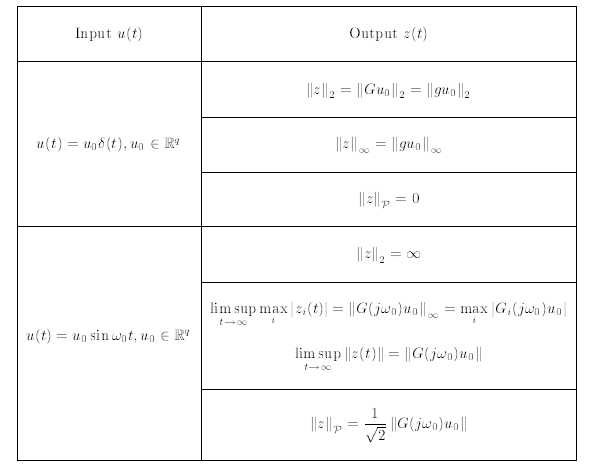
\includegraphics[scale = 0.9]{Control/Controlf1.png}
\end{figure}

Es interesante ver el significado de la tabla anterior desde el punto de vista del control. En nuestro foco de atención, asumimos que la señal de entrada $u(t)=u_0 \sin{\omega_0 t}$ es una perturbación o una señal de comando en el sistema realimentado, y la señal $z(t)$ es la señal de error. Entonces se dice que el sistema tiene un buen error de seguimiento si $z(t)$ es pequeña en algún sentido, por ejemplo, $\limsup_{t \to \infty}{||z(t)||}$. Note que

\begin{equation*}
    \limsup_{t \to \infty}{||z(t)||} = ||G(j \omega_0 )u_0||
\end{equation*}

para cualquier frecuencia dada $\omega_0$ y $u_0 \in \mathbb{R}^q$. Ahora si queremos seguir señales desde varios canales, esto es, si $u_0$ puede ser ecogido en cualquier direección, entonces se requeriría que $\bar{\sigma}( G (j \omega) )$ sea pequeño. Adicionalmente, si queremos seguir señales de muchas frecuencias distintas, entonces $\bar{\sigma}( G (j \omega) )$ deberá ser pequeño a todas esas frecuencias.\\

En la siguiente tabla se muestra la máxima ganancia posible cuando la señal de entrada no está dada como una señal fija.

\begin{figure}[H]
    \centering
    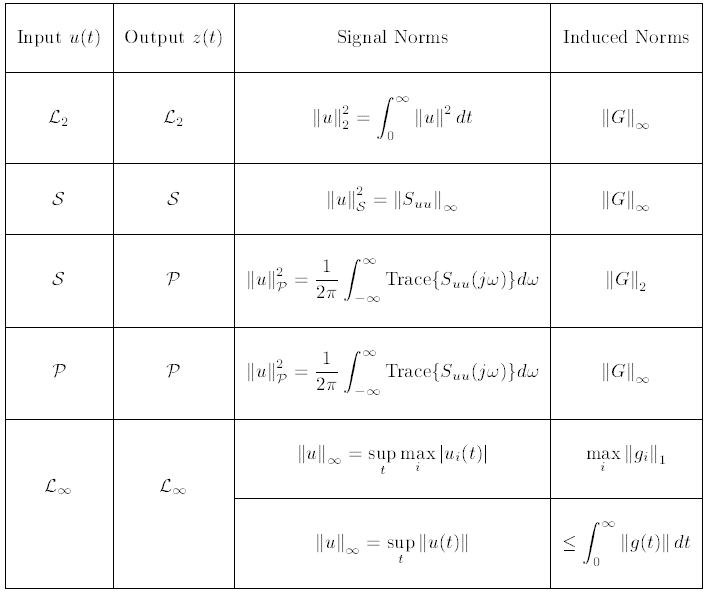
\includegraphics[scale = 0.85]{Control/controlf2.png}
\end{figure}


Derivemos algunos límites útiles para la norma $\mathcal{H}_\infty$ y la norma de $\mathcal{L}_1$ de un sistema estable, suponga que

\begin{equation*}
    G_1(s) = \left( \begin{tabular}{c|c}$A_1$&$B_1$\\\hline$C_1$&$D_1$\end{tabular} \right) \in \mathcal{R H}_\infty
\end{equation*}

es una realización balanceada, es decir, que $\Sigma = diag(\sigma_1,\sigma_2,\dots,\sigma_n) \geq 0$, con $\sigma_1 \geq \sigma_2 \geq \dots \geq \sigma_n \geq 0$ tal que

\begin{equation*}
    A \Sigma + \Sigma A^{*} + B \ B^{*} = 0
\end{equation*}


\begin{equation*}
    A^{*} \Sigma + \Sigma A + C^{*} \ C  = 0
\end{equation*}
entonces tenemos el siguiente teorema

\subsubsection{Teorema} 

\begin{equation*}
    \sigma_1 \leq ||G||_\infty \leq \int_{0}^{\infty} ||g(t)|| dt \leq 2 \sum_{i=1}^{n} \sigma_i
\end{equation*}

donde $g(t) = Ce^{At}B$

\begin{figure}[H]
    \centering
    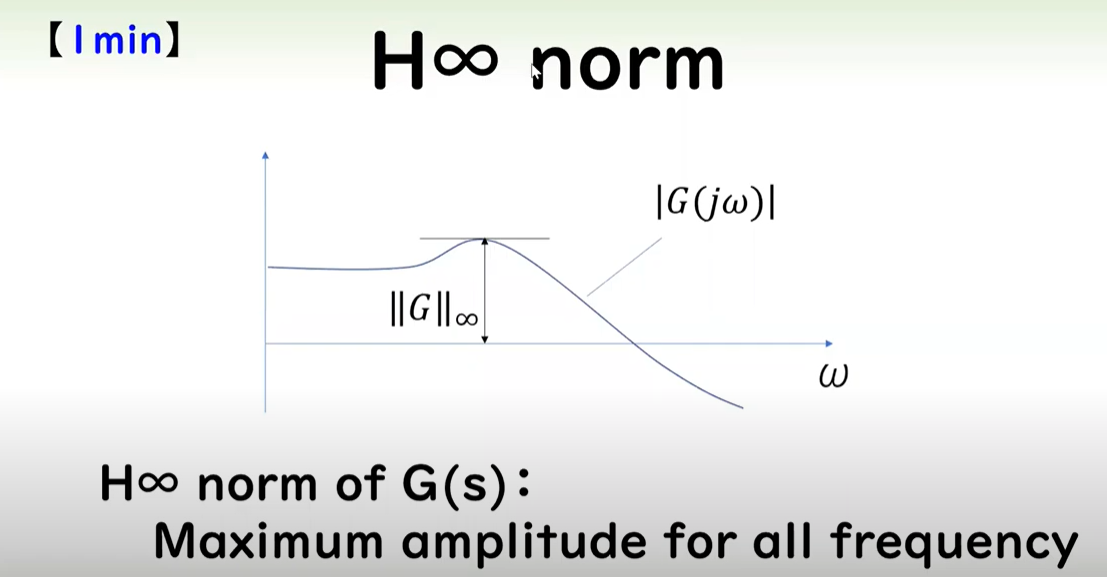
\includegraphics[scale = 0.5]{Control/controlf3.png}
\end{figure}


\section{Calculando las normas L2 y H2}

Sea $G(s) \in \mathcal{L}_2$, y recuerde que la norma $\mathcal{L}_2$ de $G$ se define como sigue

\begin{eqnarray*}
    ||G||_2 & := & \sqrt{\frac{1}{2 \pi} \int_{- \infty}^{\infty}\text{Tr}(G^{*}(j \omega) G(j \omega))d \omega} \\
    &=& ||g||_2 \\
    &=& \sqrt{\int_{- \infty}^{\infty}\text{Tr}(g^{*}(t) g(t))d \omega}
\end{eqnarray*}

donde $g(t)$ es el núcleo de convolución de $G$.

Es fácil de ver que la norma $\mathcal{L}_2$ es finita si y solo si la matriz de transferencia $G$ es estrictamente propia. Así vamos a asumir de manera general que la matriz es estrictamente propia. Una forma sencilla de calcular la norma $\mathcal{L}_2$ es usar integrales de contorno


\begin{equation*}
     ||G||_2^{2} = \frac{1}{2 \pi} \int_{- \infty}^{\infty}\text{Tr}(G^{*}(j \omega) G(j \omega))d \omega
\end{equation*}


\begin{equation*}
     ||G||_2^{2} = \frac{1}{2 \pi j} \oint \text{Tr}(G^{*}(s) G(s))d s
\end{equation*}

La anterior es una integral de contorno a lo largo del eje imaginario y al redededor del semicírculo infinito del semiplano izquierdo, la contribución a la integral de la sección de semicpirculo infinito es igual a cero dado que la matriz de transferencia es estrictamente propia. Por el teorema del residuo, $ ||G||_2^{2}$ es igual a la suma de los residuos de $\text{Tr}(G^{*}(s) G(s))$ en sus polos en el semiplano izquierdo.

Aunque la norma puede ser calculada en principio de su definición es más util en muchas aplicaciones tener una caracterización alternativa y tener ventajas de la s representaciones de espacio de estados de G. El cálculo de la norma $\mathcal{R H}_2$ de una matriz de transferencia es particularmente simple. \\

\paragraph{Lema} Considere la matriz de transferencia
\begin{equation*}
    G_1(s) = \left( \begin{tabular}{c|c}$A$&$B$\\\hline$C$&$0$\end{tabular} \right) 
\end{equation*}
Donde $A$ es estable. Entonces tenemos que 
\begin{equation*}
    ||G||_2^2 = \text{Tr}(B^{*} W_o B) = \text{Tr}(C W_c C^{*})
\end{equation*}
donde $W_o$ y $W_c$ son los gramianos de controlabilidad y observabilidad y se pueden obtener de las siguientes ecuaciones de Lyapunov
\begin{equation*}
    A W_c + W_c A^{*} + B B^{*} = 0
\end{equation*}
\begin{equation*}
    A^{*} W_o + W_o A + C^{*} C = 0
\end{equation*}



% \chapter{Visual Studio Code}

\section{Snippets personalizados}

Todos los archivos de snippets están escritos en formato JSON. Existen archivos propios para cada lenguage y existen también para uso global en VSCode. La sintaxis para configurar snippets personales es la que se muestra a continuación.

\begin{verbatim}
"title": {
    "prefix": "chapter",
    "body": "\\chapter{$1}"
}
\end{verbatim}

Los items más importantes son \texttt{"prefix"}, que indica el texto que se teclea para que intellisense reconozca el snippet y lo ejecute. El segundo es \texttt{"body"}, que indica el texto que se usa dentro del snippet. Las directivas \texttt{$1,$2,...} son usadas para ubicar el cursor para llenar las opciones dentro del snippet. También pueden tener identificadores con palabras y no solamente números.\\

Para proponer una porción de código de varias líneas, se puede usar la siguiente sintaxis

\begin{verbatim}
"Add a image": {
    "prefix": "figure",
    "body": [
        "\\begin{figure}[$1]",
        "\t\\centering",
        "\t\\includegraphics[width=$2\\columnwidth]{$3}",
        "\t\\caption{$4}",
        "\t\\label{$5}",
        "\\end{figure}",
    ],
    "description": "Add an image"
\end{verbatim} 

Se puede observar también la directiva \texttt{\textbackslash t} para proponer dentro del snippet la inclusión de identación.


\section{Edicion de texto con markdown para la documentación}


Una herramienta que puede ser útil para los repositorios es la de edición de la documentación con markdown, que con la opción \texttt{Markdown: Preview} permite ver cómo está quedando la documentación, y con la opción \texttt{Markdown: open preview on the side} para que se actualice en tiempo real.
\begin{itemize}
    \item Título principal: \texttt{\# Title} \\
    \item Título secundario: \texttt{\#\# Subtitle} \\
    \item Título de sub-sección: \texttt{\#\#\# Subsection} \\
    \item Numeración normal: \texttt{1. text}
    \item Adición de texto en formato código: \texttt{See the following code : 'sudo apt install -g typescript'} \\
    \item Inserción de una URL a una palabra en particular: \texttt{You can see the documentation in this [link](https://github.com/) } \\
\end{itemize}

Para la creación de tablas con Markdown se utilizan la barra vertical:


\begin{verbatim}
| Position | Url |
|----------|-----|
|All employees  | localshost |
\end{verbatim}








\section{Organizacion del código}

Una herramienta útil para el uso del código es la de reemplazar todas las ocurrencias para una palabra, con el comando \texttt{Ctrl + F2} se renombra todas las palabras realcionadas. Otro comando importante es \texttt{Ctrl+D} el cual selecciona solamente la palabra, en caso de querer reemplazarla o simplemente borrarla.


En ocasiones es necesario tener varias terminales para diferentes propósitos dentro del proyecto, una configuración útil para mejorar la productividad es la siguiente configuración de teclado:


\begin{verbatim}
{
    "key": "ctrl+tab",
    "command": "workbench.action.terminal.focusNext",
    "when": "terminalFocus"
}

{
    "key": "ctrl+shift+tab",
    "command": "workbench.action.terminal.focusPrevious",
    "when": "terminalFocus"
}

{
    "key": "ctrl+n",
    "command": "workbench.action.terminal.new",
    "when": "terminalFocus"
}

{
    "key": "ctrl+w",
    "command": "workbench.action.terminal.kill",
    "when": "terminalFocus"
}

{
    "key": "ctrl+r",
    "command": "workbench.action.terminal.rename",
    "when": "terminalFocus" 
}
\end{verbatim}

en el archivo \texttt{Json} de los atajos de teclado.

\section{Definición de 'workspace'}

Los entornos de trabajo son básicamente una colección de carpetas las cuales podemos manejar en una misma ventana de VSCode. Estos se guardan con la extensión \texttt{.code-workspace}. Cada espacio de trabajo se puede ver como una entidad diferente en la cual estoy realizando el trabajo de código.


\section{Notas adicionales}

\subsection{Comandos importantes}

La siguiente es una lista importante de los comandos que facilitan la productividad



\begin{itemize}
    \item \texttt{Alt + Up/Down} Mueve la línea o líneas de código hacia arriba o hacia abajo 
    \item \texttt{Shift + Alt + T} Muestra u oculta el terminal de VSCode
    \item \texttt{Ctrl + L} Selecciona toda la línea
    \item \texttt{Ctrl + D} Selecciona la palabra actual
    \item \texttt{Ctrl + F3 / Shift+Ctrl+F3} Cuando el cursor está sobre una palabra, selecciona la palabra y mueve el cursor hacia la siguiente lalabara duplicada.
    \item \texttt{Shift+Alt+K} Borra la línea completa
    \item \texttt{Ctrl+Shift+E} Abre el explorador de la parte izquierda
    \item \texttt{Ctrl+Shift+L} Selecciona todas las palabras repetidas
    \item \texttt{Ctrl+Shift+M} Abre o cierra el panel de problemas de la parte inferior
    \item \texttt{Ctrl+Shift+Y} Abre o cierra la consola de debug de la parte inferior
    \item \texttt{Ctrl+Shift+U} Abre o cierra el panel de salida de la parte inferior
    \item \texttt{Ctrl+Enter} Hace un salto de línea si importar en qué parte de lña línea se encuentre
    \item \texttt{Shift+Enter} Ejecuta el script
    \item \texttt{Ctrl+Tab} CAmbia entre pestañas abiertas
    \item \texttt{Shift+Alt+A} Comentar/quitar comentario de un bloque de código seleccionado
    \item \texttt{Ctrl+\}} Comentar/quitar comentario de una línea
    Si en el buscador al que accedemos con \texttt{Ctrl+Shift+P} ponemos dos puntos seguidos con un número, automáticamente se va a seleccionar esa línea de código.
    \item \texttt{Ctrl+B} Muestra o quita la barra de la izquierda (Explorador,Extensiones, etc)
    \item \texttt{F2} al tener una palabra seleccionada, si se trata de una dofinición de clase, o una palabra repetida, sirve para cambiar esa definición y se cambiarán todas las ocurrencias de esa palabra.
    \item \texttt{Shift+Alt+Up/Down} coia la línea entera de código en la línea siguiente o en la linea anterior.
\end{itemize}

\subsection{Concepto de tareas}

 

Las tareas en VSCode son una herramienta que sirve para automatizar procesos dentro de VSCode. La creación y ejecución de tareas está manejado mediante archivos JSON. En estos se configura la lista de tareas que serán ejecutadas cuando la tarea asea ejecutada.


\subsection{Debug} 
También es posible personalizar una configuración JSON para ejecutar el programa con el depurador.
\chapter{Datos}


\section{Modelo de datos}


¿Qué es un modelo de datos?

Es un conjunto de tablas de datos que tienen relaciones y conexiones entre sí. Lo importante es que existan relaciones entre las diferentes tablas; relaciones de conexión entre datos como columnas o datos claves en común.

\subsection{Normalización de los datos}

Es el proceso de organización de las tablas y las columnas en una base de datos relacional para reducir la redundancia y preservar la integridad de los datos.

\begin{itemize}
    \item la eliminación de los datos para reducir el tamaño de las tablas y aumentar la velocidad y eficiencia.
    \item MInimizar las anomallías y los errores de las modificaciones de los datos.
    \item simplificación de las consultas y estructuración de la base de datos para análisis más útiles.
\end{itemize}

una buena manera de entender una base de datos normalizada es definiéndola de la siguiente manera: en una base de datos normalizada, cada tabla debe tener un \textbf{propósito único y específico}. \\

los modelos tienen generalmente dos tipos de tablas

\begin{enumerate}
    \item Tablas de datos: contiene números o valores, típicamente a nivel granular, con una columna de identificación o Id que puede ser
    \item Tablas de Vista: provee atributos descriptivos normalmente basados een texto sobre cada dimensión de la tabla. en este caso, este tipo de tablas provee mucha información sobre objetos como pueden ser "clientes" o "Productos".
\end{enumerate}

\subsection{Expresiones de análisis de datos}


Las expresiones de análisis de datos o DAX son un lenguage de fórmilas de PowerBI. Con estas fórmulas se puede hacer lo siguiente:

\begin{itemize}
    \item Añadir columnas con cálculos y mediciones al modelo, usando sintaxis intuitiva.
    \item Ir más alla de las capacidades de las formulas tradicionales, con funciones potentes y flexibles construidas específicamente para trabajar con modelos de datos relacionales.
\end{itemize}

Existen dos maneras de realizar acciones DAX: mediante creación de columnas nuevas, y mediante mediciones de un solo valor.


\subsubsection{Columnas calculadas}

Se pueden agregar columnas nuevas basadas en fórmulas a las tablas. Cosas importantes a remarcar:

\begin{enumerate}
    \item No hay referencias a celdas, todas las columnas calculadas se referencian a tablas enteras o a columnas enteras
    \item Las columnas calculadas generan valores por cada fila, los cuales son visibles dentro de las tablas en la vista de datos.
    \item Las columnas calculadas entienden el conexto de filas, lo que significa que son muy útiles para definir propiedades que estén basadas en la información de cada fila.
\end{enumerate}

Como un tip adicional y útil, use las columnas calculadas para \textbf{filtrar datos} más que para cear valores numéricos.


\paragraph*{Ejemplo}

\begin{verbatim}
    Parent = IF(Customer_Lookup[TotalChildren]>0, "Yes", "No")
\end{verbatim}

En este ejemplo se puede usar un if condicionante para agregar una columna nueva de control o de filtro.


\subsubsection{Mediciones}

En este caso son usados para generar nuevos valores calculados.

\begin{enumerate}
    \item Igual que la anterior, no hay forma de referenciar celdas aisladas; solo para tablas enteras.
    \item Estos valores no pueden ser visibles dentro de las tablas, solamente se pueden ver en elementos de visualización como cartas, o matrices.
    \item Estos cálculos siempre estarán regidos por el contexto del filtro; es decir, el valor se recalcula siempre que sea aplicado algún filtro en el elemento de visualización que se agrege o configure.
\end{enumerate}

A manera de regla general, use este tipo de cálculo cuando una única fila no puede entregarle el valor solicitado. En otras palabras, cuando necesite más de una fila.

\subsubsection{Mediciones implícitas y explícitas}

Las mediciones implícitas están en los elementos de visualización cuando uno arrastra un campo numérico a dicho elemento. Ahí es cuando se puede seleccionar el modo de agregación (suma, media, mínimo, máximo, etc.

Las mediciones explícitas, son por el contrario las que se definen de manera literal con la sintaxis de DAX

Recordando que las mediciones son evaluadas con base en el contexto de filtrado, según el filtro aplicado el resultado de la medición sera distinta. 

Por ejemplo, para la siguiente imagen, el valor sombreado es la suma del campo "Valor" está canlculado con base en el siguiente contexto de filtro: \texttt{IDLookup[Nombre]="Pago Obligatorio"}

\begin{figure}[H]
    \centering
    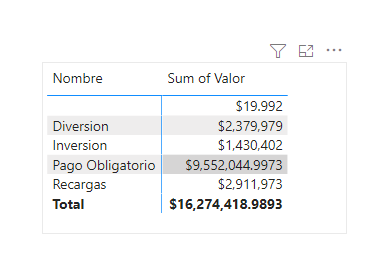
\includegraphics[scale=0.6]{Data/datafig2.png}
\end{figure}



% \begin{verbatim}
%     Overall Avg Price = CALCULATE([Avg Retail Price],ALL(AW_Products_Lookup))
% \end{verbatim}

% quita cualquier filtro de la tabla \texttt{AW\_Products\_Lookup} para tener el valor total de \texttt{Avg Retail Price} en \textbf{todas las filas}. \\

% \subsubsection*{Ejemplo de uso de filter}

% Si queremos sacar una medida de, por ejemplo, las ventas de un producto cuyo precio está por encima del promedio. \\

% \begin{verbatim}
%     High Ticket Order = CALCULATE([Total Orders], FILTER(AW_Products_Lookup,AW_Products_Lookup[ProductPrice] > [Overall Avg Price]))
% \end{verbatim}

% Aquí lo que se hace es que se pone la función filter en el filtro, el primer argumento de filter es la tabla que vamos a filtrar y el segundo argumento es la cindición de filtro.

% \begin{verbatim}
% Total Revenue_Measure = SUMX(AW_Sales,[Quantity Sold]*AW_Sales[RetailPrice])
% \end{verbatim}

% EN este caso se hace la suma total de todos los resultados de multiplicar \texttt{retailPrice} por \texttt{QuiantitySold}, como un producto punto.


% \begin{verbatim}
% Total Revenue_Measure = SUMX(AW_Sales,AW_Sales[OrderQuantity] * RELATED(AW_Products_Lookup[ProductPrice]))
% \end{verbatim}

% Esta lo que hace es traer a mi tabla de ventas, los datos relacionadosque vengan de la tabla de productos, para calcular el valor de los precios.\\

% Las siguientes son algunas fórmulas de tiempo inteligentes que pueden ser útiles: \\

% \texttt{CALCULATE(Measure, DATEYTD(Calendar[Date]) )} Si aplicamos este filtro a una medición de suma total de ingresos de ventas y ponemos en las filas los primeros días de cada mes, entonces obtenemos \\


% \texttt{YTD Revenue = CALCULATE([Total Revenue\_Measure], DATESYTD(AW\_Calendar\_Lookup[Date]))}

% Obtenemos los datos de ganancias mensualkes hasta el final de año y se inicia de nuevo en cada año

% \begin{figure}[H]
%     \centering
%     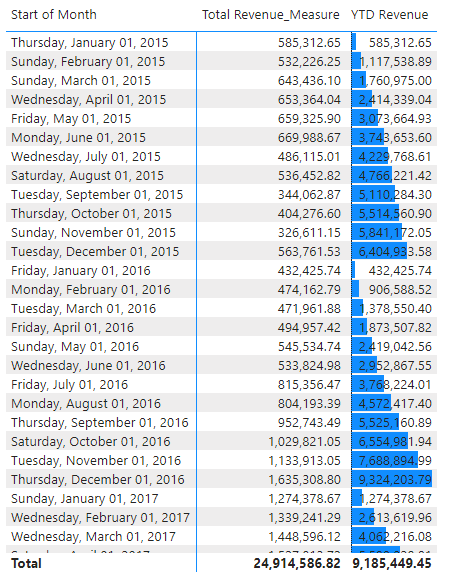
\includegraphics[scale=0.6]{Data/data1.png}
% \end{figure}



 

\texttt{CALCULATE(Measure, DATEADD(Calendar[Date], -1 , MONTH) )} Aquí la función DATEADD devuelve un rango de fechas desplazado en la cantidad y con intervalos puestos en sus argumentos \\ 
\texttt{CALCULATE(Measure, DATESINPERIOD(Calendar[Date],MAX(Calendar[Date]), -1, DAY) )} \\









\subsubsection{Sintaxis de las expresiones DAX}

Las sentencias de las expresiones se pueden separar en tres partes diferentes: nombre de la medición realizada, nombre de la función, y las referencias o argumentos de las funciones, estas pueden referirse al nombre de la tabla con su respectiva columna. También se puede estar refiriendo a una medición anteriormente definida. Como tip de utilidad, cuando nos vayamos a referir a referecias de columnas, usamos el nombre: \texttt{Table[Column]}. Y para referencias a mediciones, solo usamos el nombre de la medición: \texttt{Measure}.


Algunos operadores importantes los podemos ver en la siguiente tabla

\begin{table}[H]
    \centering
    \begin{tabular}{|c|c|c|}
        \hline
        Operador & Significado & Ejemplo\\ \hline
        + & Suma & 2 + 7 \\ \hline
        - & Resta & 5 - 3 \\ \hline
        * & Multiplicación & 2 * 6 \\ \hline
        / & División & 2 / 4 \\ \hline
        $\wedge$ & Exponente & 5 $\wedge$ 5 \\ \hline
        = & Igual a & [City] = "Boston"\\ \hline
        $>$ & Mayor & [Quantity] > 10\\ \hline
        $<$ & Menor que & [Quantity] < 10 \\ \hline
        $>=$ & Mayor o igual & [Unit\_Price] >= 2.5 \\ \hline
        $<=$ & Menor o igual & [Unit\_Price] <= 2.5 \\ \hline
        $<>$ & Diferente a & [Country] <> "Mexico" \\ \hline
        \& & Concatena dos caracteres o cadenas para formar una nueva & [City] \& "" \& [State] \\ \hline
        \& \& & AND & ([State]="MA") \& \& ([Quantity]>10) \\ \hline
        $||$ & OR & ([State]="MA") $||$ ([State]="CT") \\ \hline
        IN & Crea una condición lógica OR basada en una lista dada. & 'Store Lookup'[State] IN {"MA", "CT", "NY"} \\ \hline
    \end{tabular}
\end{table}


Las funciones también las podemos clasificar en diferentes categorías:

\begin{enumerate}
    \item Math and stats

        Tenemos aquí las funciones matemáticas de agregación más básicas y también algunas iteradoras:
        \begin{itemize}
            \item SUM
            \item AVERAGE
            \item MAX/MIN
            \item DIVIDE
            \item COUNT/COUNTA
            \item COUNTROWS
            \item DISTINCTCOUNT
            \item SUMX
            \item AVERAGEX
            \item MAXX/MINX
            \item RANKX 
            \item COUNTX
        \end{itemize}
    \item Logical functions

        Estas funciones generalmente tienen la tarea de retornar información sobre valores, con base en una expresión condicional dada. usualmente o mayoritariamente basadas en condicionales "if":
        \begin{itemize}
            \item IF
            \item IFERROR
            \item AND
            \item OR
            \item NOT
            \item SWITCH
            \item TRUE
            \item FALSE
            
        \end{itemize}
        
    \item Text functions

        Son funciones que sirven para manipular texto o formatos de control para fechas, horas o números

        \begin{itemize}
            \item CONCATENATE
            \item FORMAT
            \item LEFT/MID/RIGHT
            \item UPPEER/LOWER
            \item PROPER
            \item LEN
            \item SEARCH/FIND
            \item REPLACE
            \item REPT
            \item SUBSTITUTE
            \item TRIM
            \item UNICHAR
        \end{itemize}
    
    \item Filter functions

        Estas son funciones que están basadas en tablas relacionadas y para filtrar funciones para cálculos dinámicos.

        \begin{itemize}
            \item CALCULATE
            \item FILTER
            \item ALL
            \item ALLEXCEPT
            \item RELATED
            \item RELATEDTABLE
            \item DISTINCT
            \item VALUES 
            \item EARLIER/EARLIEST
            \item HASONEVALUE
            \item HASONEFILTER
            \item ISFILTERED
            \item USERELATIONSHIP
        \end{itemize}
        
    \item Date and time functions

            Estas son funciones especializadas en fechas y horas, así como operaciones inteligentes avanzadas
            \begin{itemize}
                \item DATEDIFF
                \item YEARFRAC
                \item YEAR/MONTH/DAY
                \item HOUR/MINUTE/SECOND
                \item TODAY/NOW
                \item WEEKDAY/WEEKNUM
                \item DATESYTD
                \item DATESQTD
                \item DATESMTD
                \item DATEADD
                \item DATESINPERIOD
            \end{itemize}
\end{enumerate}


Un par de funciones muy útiles para el manejo de las fechas son \texttt{weekday/weeknum()} y \texttt{eomonth()}. La primer función retorna el número del día de la semana de la fecha que se ponga como argumento. Por defecto, el número 1 será el día domingo, pero esto se puede cambiar mediante una opción. La segunda retorna la fecha correspondiente al último día del mes, más o menos un número especificado de meses.\\

Una de las funciones más importantes o útiles puede ser \texttt{RELATED} la cual retorna valores relacionados directamente con cada fila con base en la relación que haya con otras tablas. La sintaxis de la función es:

La función \texttt{DATEADD} Devuelve la fecha que resulta de restar o sumar la cantidad especificada en el argumento.


\begin{verbatim}
    =RELATED(ColumnName)
\end{verbatim}

el nombre de la columna es la columna de la cual se requiere extraer la información o el dato. Como tip es recomendable tratar de no crear nuevas columnas basadas en esta función, en algunas osiones esto puede ser redundante; es más recomendable usar este tipo de funciones dentro de otras como iteradores del tipo \texttt{SUMX}.



\begin{verbatim}
DATEADD(Calendar[date],-1,MONTH)
\end{verbatim}

La anterior devuelve la fecha restada en un mes

Teniendo en cuenta la tabla de gastos personal, si usamos la siguiente función:

\begin{verbatim}
YTD Gastos = CALCULATE(SUM(Gasto[Valor]), DATESYTD(Calendario_Lookup[Fecha]))
\end{verbatim}

obtenemmos la suma acumulativa de los gastos y se "renueva" en año nuevo. Observar como las barras van aumentando y el valor acumulado en el año.

\begin{figure}[H]
    \centering
    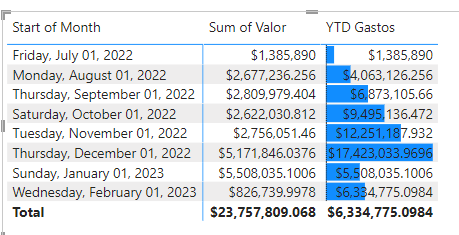
\includegraphics{Data/datafig3.png}
\end{figure}

\subsection{Parámetros 'what if'}

Este tipo de parámetros son esencialmente parámetros DAX preconfigurados que producen valores dentro de un rango dado. Este tipo de medidas pueden ser muy útiles por ejmplo para estudios de pronósticos o para estudios de posibles escenarios. para más información revisar la lección 98 del curso.


\section{SQL}



    \subsection{Conceptos}

    \subsubsection{Query}

    Es una porción de código que induce a la computadora a ejecutar una serie de operaciones y que entregará la salida requerida.


    SQL Es un lenguaje de programación declarativo no procedural. No se focaliza tanto en el procedimiento como en cuál es la tarea que se está solicitando. Su sintaxis se compone principalmente de 

    \begin{itemize}
        \item Lenguaje de definición de datos
        \item Lenguaje de manipulación de datos
        \item Lenguaje de control de datos
        \item Lenguaje de control de transacciones
    \end{itemize}

    \texttt{CREATE object\_type object\_name} \\

    \texttt{CREATE TABLE object\_name (column\_name data\_type)} \\


    \texttt{CREATE TABLE sales (purchase\_number INT data\_type)} creará una tabla llamada sales con una columna llamada purchase number del tipo entero.

    \begin{verbatim}
    ALTER TABLE sales
    ADD COLUMN date_of_purchase DATE;
    \end{verbatim}

    Se modifica la tabla agregando una columna nueva.

    \texttt{DROP TABLE customers;} borra la tabla entera \\


    \texttt{RENAME TABLE customers TO customer\_data;} cambia el nombre de la tabla. \\

    \texttt{TRUNCATE} borra los datos enteros de una tabla, pero la tabla sigue existiendo \\

    Ahora algunas palabras reservadas de DML (lenguaje de manipulación de datos)

    \texttt{SELECT .. FROM sales} selecciona lo indicado de la tabla de ventas. Se ua para extraer información de la tabla


    \texttt{INSERT INTO sales (purchase\_number, date\_of\_purchase) VALUES(1, '2017-10-11');} añade datos a la tabla

    \begin{verbatim}
    UPDATE sales 
    SET date_of_purchase = '2017-12-11'
    WHERE purchase_number = 1;
    \end{verbatim}

    Cambia directamente una entrada de la tabla


    \begin{verbatim}
    DELETE FROM sales
    WHERE
        purchase_number = 1;
    \end{verbatim}


    Sentencias para control de datos

    \begin{verbatim}
    GRANT type_permission ON database_name.table_name TO 'username'@'localhost'
    \end{verbatim}

    Otorga permisos determinados a los usuarios


    \begin{verbatim}
    REVOKE type_permission ON database_name.table_name TO 'username'@'localhost'
    \end{verbatim}

    Quita los permiso. \\

    Finalmente los comandos de control de transacciones

    \texttt{COMMIT} solamente funciona cuando se hacen cambios del tipo \texttt{INSERT}, \texttt{DELETE}, o \texttt{UPDATE}.


    \begin{verbatim}
    UPDATE customers
    SET las_name = "Johnson"
    WHERE customer_id = 4
    COMMIT;
    \end{verbatim}


    \texttt{ROLLBACK} permite devolver al estado anterior de commit

    \subsection{Pasos para crear una database y usarla}

    \begin{verbatim}
    create database if not exists Sales; 
    use Sales
    \end{verbatim}
    EL lenguaje SQL no es sensible a mayúsculas-minúsculas, ni para los nombres de los diferentes objetos, ni para las solicitudes. Esto quiere decir que \texttt{sales} y \texttt{Sales} serán iguales para SQL

    \subsection{Tipos de datos}
    Siempre es necesario especificar el tipo de datos que se insertará en cada columna de la tabla.
    \subsubsection{Cadenas de caracteres}

    Existen varios tipos de cadenas string. 

    \begin{enumerate}
        \item caracter: \texttt{CHAR}, tiene un tamaño de almacenamiento fijo y depende de qué tamaño sea declarado. \texttt{CHAR(5)} tendrá un tamaño de 5 bytes aunque el string tenga menos de 5 símbolos. 
        \item caracter variable: \texttt{VARCHAR} en este caso el tamaño de la variable no está fijo, así un \texttt{VARCHAR(5) = 'bob'} tendrá un tamaño de 3 bytes.
        \item \texttt{ENUM} Es un tipo de variable que contiene un conjunto definido total de cadenas. Por ejemplo, para el género, cuando solamente hay dos opciones para seleccionar, se puede declarar la variable \texttt{ENUM('M','F')}.
    \end{enumerate}

    Una cadena de caracteres char puede tener un tamaño máximo de 255 bytes. Un \texttt{varchar}, por su parte, puede tener un tamaño máximo de 65535 bytes. El procesamiento de las variables \textit{char} es más rápido y eficiente que el de las \texttt{varchar}, razón por la cual a veces es más conveniente declarar las primeras. \\ 

    \subsubsection{Enteros}

    La siguiente tabla resume los diferentes tipos de enteros que se pueden declarar y sus tamaños máximos así como los valores máximos que pueden tomar

    \begin{table}[H]
        \centering
        \begin{tabular}{c|c|c|c|}
        \hline
            Tipo & Tamaño & Valor mínimo (con signo/sin signo) & Valor máxumo (con signo/sin signo)  \\ \hline
            \texttt{ TINYINT }  & 1  & -128/0  & 127/255\\ \hline
            \texttt{ SMALLINT } & 2  &  -32 768/0 & 32 767/65 535\\ \hline
            \texttt{ MEDIUMINT }& 3  &  -8 388 608/0 & 8 388 607 / 16 777 215 \\ \hline
            \texttt{ INT }      & 4  & -2 147 483 648 /0  & 2 147 483 647 / 4 2094 967 295 \\ \hline
            \texttt{ BIGINT }   & 8  & -9 223 372 036 854 775 808 / 0 &  9 223 372 36 854 775 807 / 18 446 744 73 709 551 615\\ \hline
        \end{tabular}
    \end{table}

    \subsection{Variables de puntos flotantes y puntos fijos}

    En este contexto la precisión de un número se refiere a la cantidad de dígitos que hay en el mismo. Por ejemplo, \texttt{10.523} tiena una precisión de 5. Por su parte, la escala de la variable se refiere a la cantidad de dígitos que hay después del punto decimal. en el ejemplo anterior, la escala es de 3.

    Es importante saber la diferencia entre datos de punto fijo y datos de punto flotante. Los datos de punto fijo son los que representan valores exactos. Existen dos tipos de variables para los puntos fijos:

    \begin{verbatim}
    DECIMAL(5,3)
    NUMERIC
    \end{verbatim}
    Para el ejemplo \texttt{decimal(5,3)} cualquier número insertado en esta variable contendrá esta estructura. Si se inserta un \texttt{10.5} el número en realidad será \texttt{10.500}, y si se agrega un número con más decimales, entonces se redoneará para que pueda entrar en la variable, se saltará una advertencia.

    Un buen ejemplo de uso de este tipo de datos son los valores monetarios: Salarios, gastos, etc. \texttt{NUMERIC(p,s)} donde \texttt{p} representa la precisión y \texttt{s} representa la escala.


    Por su parte, los datos de coma flotante se usan para aproximar valores solamente y tiene como objetivo equilibrar el alcance y la precisión, Simplemente aproxima el valor y guarda esa aproximación. En este caso tenemos los siguientes tipos de variables para los números de coma flotante.

    \begin{verbatim}
    FLOAT
    DOUBLE
    \end{verbatim}

    \texttt{float} tiene un tamaño de 4 bytes. Es de precisión sencilla y cuenta con un máximo de 23 dígitos.  \\
    \texttt{float} tiene un tamaño de 8 bytes. Es de precisión doble y cuenta con un máximo de 53 dígitos.  \\

    \subsection{Otros tipos de datos}

    \begin{itemize}
        \item \texttt{DATE} el formato es YYYY-MM-DD. La hora no hace parte de esta representación
        \item \texttt{DATETIME} El formato es YYYY-MM-DD HH:MM:SS[.fraction]. El rango de la hora es \texttt{0 - 23:59:59.999999}
        \item \texttt{TIMESTAMP} Es el conteo en segundos desde una fecha inicial, sirve como punto de comparación entre dos fechas y establecer la diferencia en tiempo
        \item \texttt{BLOB} Significa binary large object. Se puede usar para guardar archivos de difrentes tipos: objetos binarios de gran tamaño. como fotos. 
        \item \texttt{}
    \end{itemize}


    
    \subsection{Creación de tablas}
    
    
    \begin{verbatim}
        CREATE TABLE table_name
        (
            column_1 data_type constraints,
            .
            .
            .
            column_n data_type constraints
        );
    \end{verbatim}
    
    
    Ejemplo:
    
    \begin{verbatim}
    CREATE TABLE Sales
    (
        purchase_name int not null primary key auto_increment,
        date_of_purchase date not null,
        customer_ID int,
        item_code varchar(10) not null
    );
    \end{verbatim}
    
    la sentencia \texttt{auto\_increment} asigna el número de ID a esta columna y la aunemta automáticamente. \\

    \begin{verbatim}
    CREATE TABLE Customers
    (
        customer_ID int not null primary key auto_increment,
        first_name varchar(255) not null,
        last_name varchar(255) not null,
        email_address varchar(255),
        number_of_complaints int
    );
    \end{verbatim}



    \subsection{Restricciones de SQL}

    Las restricciones son especificaciones de reglas o límites que se imponen a cada una de las columnas de la tabla. Los términos "primary key" (clave primaria) y "foreign key" (clave foránea) son fundamentales para entender cómo se relacionan las tablas entre sí y cómo se mantiene la integridad de los datos.

    \subsubsection{\texttt{primary key}}

    Una clave primaria es un campo (o conjunto de campos) que identifica de manera única cada fila en una tabla de una base de datos. Las características principales de una clave primaria son:

    \begin{enumerate}
        \item \textbf{Unicidad}: Ningún valor duplicado es permitido en una clave primaria. Cada fila debe tener un valor único para la clave primaria.
        \item \textbf{No nula}: Una clave primaria no puede tener valores nulos. Cada fila debe tener un valor para la clave primaria.
        \item \textbf{Identificación}: La clave primaria se utiliza para identificar de manera exclusiva una fila en la tabla.

    

    
    \end{enumerate}
    
    Una forma de asignar una clave primaria a una tabla es la siguiente:

    \begin{verbatim}
    CREATE TABLE Sales
    (
        purchase_number int auto_increment,
        date_of_purchase date,
        customer_ID int,
        item_code varchar(10),
    primary key (purchase_number)
    );
    \end{verbatim}
    
    
    Creamos las demás tablas con sus respectivas claves primarias:
    
    \begin{verbatim}
    create table customer
    (
        customer_id int,
        first_name varchar(255),
        last_name varchar(255),
        number_of_complaints int,
    primary key c(ustomer_id)
    );
    \end{verbatim}
    \subsubsection{\texttt{Clave foránea}}

    Una clave foránea es un campo (o conjunto de campos) en una tabla que se utiliza para referenciar la clave primaria de otra tabla. La relación entre la clave foránea y la clave primaria es lo que permite establecer relaciones entre tablas. Las características principales de una clave foránea son: 

    \begin{enumerate}
        \item \textbf{Correspondencia} con la clave primaria: Una clave foránea en una tabla corresponde a una clave primaria en otra tabla.
        \item \textbf{Integridad referencial}: La clave foránea ayuda a mantener la integridad referencial entre las tablas, asegurando que la relación entre ellas sea válida. Por ejemplo, si una fila en una tabla A hace referencia a otra fila en una tabla B, entonces la fila referenciada debe existir en la tabla B.
        \item \textbf{Valores nulos}: A diferencia de las claves primarias, las claves foráneas pueden tener valores nulos, lo que indica que no hay una relación con otra tabla.
    \end{enumerate}

    En el contexto de bases de datos relacionales, los términos "tabla padre" y "tabla hija" son fundamentales para entender cómo se estructuran y relacionan los datos. Estos conceptos están intrínsecamente vinculados a las relaciones entre tablas, en particular a través del uso de claves primarias y foráneas.

    \paragraph{Tabla Padre:} Una tabla padre, en una relación de base de datos, es aquella que tiene una clave primaria referenciada por otra tabla. La característica clave de una tabla padre es que proporciona el registro principal o la fuente de datos que otras tablas referencian. Las propiedades de una tabla padre son :

    \begin{enumerate}
        \item \textbf{Posee una Clave Primaria}: Es esencial que tenga una clave primaria, que es un identificador único para cada fila de la tabla .
        \item \textbf{Independencia}: La tabla padre puede existir en la base de datos sin la necesidad de tener una tabla hija asociada. Sus registros no dependen de la existencia de registros en otra tabla.
        \item \textbf{Fuente de Referencia}: Otras tablas (tablas hijas) hacen referencia a la tabla padre a través de sus claves foráneas, estableciendo así una relación.
    \end{enumerate}

    \paragraph{Tabla Hija:} Una tabla hija es aquella que contiene una clave foránea que hace referencia a la clave primaria de otra tabla (la tabla padre). Las características de una tabla hija son
    \begin{enumerate}
        \item \textbf{Posee una Clave Foránea}: Contiene al menos una clave foránea que establece una relación con la clave primaria de la tabla padre.
        \item \textbf{Dependencia Referencial}: La existencia de registros en la tabla hija generalmente depende de los registros en la tabla padre. Por ejemplo, no se puede insertar un registro en la tabla hija si no existe un registro correspondiente en la tabla padre, a menos que la clave foránea permita valores nulos.
        \item \textbf{Integridad Referencial}: La clave foránea asegura que las relaciones entre la tabla hija y la tabla padre sean válidas y coherentes.
    \end{enumerate}

    La forma de definir una clave foránea es 

    \begin{verbatim}
    create table sales
    (
        purchase_number int auto_increment,
        date_of_purchase date,
        customer_id int,
        item_code varchar(10),
    primary key(purchase_number),
    foreign key(customer_id) references customers(customer_id)
    );
    \end{verbatim}
    Donde la referencia se hace a la tabla que tenga esa clave como la primaria. Hay una restricción adicional llamada \texttt{on delete cascade}. Esta cláusula indica al sistema que si se elimina en la tabla padre una entrada o fila, entonces todas las entradas de la tabla hija que hagan referencia a esa clave también deberán ser borradas. 

    Se pueden modificar las características de las tablas sin necesidad de borrarlas para añadirlas nuevamente, mediante \texttt{alter}

    \begin{verbatim}
    alter table name
    add foreign key;
    drop primary key
    \end{verbatim}
    De la misma forma se puede eliminar cualquier restricción o característica.

    \subsubsection{\texttt{Clave única}}

    La restricción \verb|UNIQUE KEY|  es un tipo de restricción que se puede aplicar a una o más columnas de una tabla para asegurar que cada fila de esa columna (o combinación de columnas) tenga un valor único dentro de la tabla. Es decir, no se pueden tener dos o más filas con el mismo valor en la(s) columna(s) marcada(s) como \verb|UNIQUE|. Un ejemplo clásico de esta restricción es una columna de correos electrónicos; que no necesariamente constituye la clave principal, pero no puede ser duplicado, aunque pueden haber filas con valores en blanco en esta columna.

    Para borrar una clave única de una tabla se debe usar
    \begin{verbatim}
    drop index name;
    \end{verbatim}
    La instrucción \texttt{DROP INDEX} para eliminar una clave única \texttt{UNIQUE KEY} puede parecer inicialmente confusa, pero tiene sentido si consideramos cómo se implementan las claves únicas internamente en los sistemas de gestión de bases de datos.

    \paragraph{Implementación de Claves Únicas como Índices} Cuando se define una \texttt{UNIQUE KEY} en una tabla, la mayoría de los sistemas de bases de datos automáticamente crean un índice único para esa clave. Este índice único es lo que efectivamente garantiza la restricción de unicidad, asegurando que no se puedan insertar valores duplicados en la columna o conjunto de columnas designadas. pero ¿Por Qué Se usa \texttt{DROP INDEX}?

    \begin{enumerate}
        \item \textbf{Índices Únicos Subyacentes}: Dado que las claves únicas son implementadas internamente como índices únicos, la eliminación de una restricción de clave única implica la eliminación del índice asociado.
        \item \textbf{Consistencia con Otros Tipos de Índices:} Los RDBMS suelen tratar las claves únicas de manera similar a otros índices (como los índices normales o los índices de texto completo). Por lo tanto, se utiliza un comando común \texttt{DROP INDEX} para eliminar cualquier tipo de índice, ya sea que haya sido creado para una clave primaria, una clave única, o para optimización de consultas.
        \item \textbf{Simplificación de la Sintaxis SQL:} Utilizar un comando común para eliminar índices, independientemente de su tipo, simplifica la sintaxis del lenguaje SQL y hace que el manejo de la base de datos sea más uniforme y predecible.
    \end{enumerate}

    \subparagraph{Consideraciones Adicionales:} Es importante mencionar que la sintaxis exacta para eliminar una clave única puede variar entre diferentes sistemas de bases de datos. Algunos sistemas pueden ofrecer una sintaxis que permite eliminar directamente una clave única sin referirse explícitamente al índice. Por su parte, eliminar una clave única (y por lo tanto, el índice único asociado) debe hacerse con cuidado, ya que altera las restricciones de integridad de la tabla y puede afectar el rendimiento de las consultas.


    \subsubsection{Por defecto}

    La restricción \texttt{default} sirve para asignar un valor particular a cualquier fila de una columna; una forma de establecer un valor predeterminado para los casos en que no se especifica un valor particular al momento de añadir filas en la tabla. \texttt{number\_of\_complaints int default 0}.  Para modificar una columna y configurar su valor por defecto, se puede mediante la siguiente forma:
    \begin{verbatim}
    alter table name
    change column old_name new name new constraint;
    alter column col_name drop constraint;
    \end{verbatim}
    Las sentencias  \verb|ALTER TABLE ... CHANGE COLUMN| y \verb|ALTER TABLE ... ALTER COLUMN| son utilizadas para modificar las características de las columnas, pero tienen propósitos y comportamientos distintos. 

    \texttt{CHANGE COLUMN} se usa principalmente para cambiar el nombre de la columna, y también permite cambiar el tipo de datos de la columna y agregar o modificar restricciones.  Por su parte, \texttt{ALTER COLUMN} se usa para modificar restricciones o configuraciones de la columna ; específicamente para camiar aspectos como el valor por defecto o para modificar la capacidad de aceptar valores nulos. A diferencia de \texttt{change column}, \texttt{alter column} no se usa para cambiar el nombre de la columna o su tipo de datos.

    Hay una tercera, llamada \verb|MODIFY COLUMN|: Usado para cambiar el tipo de datos de una columna y modificar o agregar restricciones, pero sin cambiar el nombre de la columna.

    \subsubsection{\texttt{NOT NULL}}
    Esta restricción para una columna impide que una entrada nueva esté vacía; es decir, debe tener algún valor siempre. 

    \subsection{Buenas prácticas}

    Es evidente la importancia de realizar siempre un código limpio y bien entendible, organizado, cuyas secciones sean fácilmente intercambiables. Al momento de declarar nombres, asegurarse de que sean nombres cortos, con significado acorde a su función, que brinde información sobre sí mismo, que sea pronunciable. 
    La convención clásica indica que aunque SQL no distingue mayúsculas de minúsculas, es buena práctica usar mayúsculas para escribir palabras reservadas y tipos de instrucciones, y minúscula para los nombres, nunca usar espacios, y separar palabras por guión bajo.
    \subsection{Manipulación de datos}

        Una de las declaraciones más importantes en el mundo de SQL es \texttt{SELECT}. 
        \subsubsection{ \texttt{SELECT}}
        Es una declaración que permite extraer una fracción del conjunto de datos. Permite obtener datos de las tablas. Básicamente se trata de una instrucción que se usa para solicitar datos de la base de datos. La sintaxis es la siguiente:
        \begin{verbatim}
        SELECT col_1, col_2, ...
        FROM table_name;
        \end{verbatim}
        Hay una cláusula dentro de la declaración denominada \texttt{WHERE}, la cual permite establecer una condición sobre la cual se puede especificar qué parte de los datos se requiere obtener
        \begin{verbatim}
        SELECT col_1, col_2, ...
        FROM table_name
        WHERE condition;
        \end{verbatim}
        La condición puede ser cualquier valor de verdad: \texttt{WHERE first\_name = 'Denis'}. Los operadores de verdad son 

        \begin{itemize}
            \item \texttt{=}
            \item \texttt{AND}
            \item \texttt{OR}
            \item \texttt{IN}
            \item \texttt{NOT IN}
            \item \texttt{LIKE}
            \item \texttt{NOT LIKE}
            \item \texttt{BETWEEN... AND..}
            \item \texttt{EXISTS}
            \item \texttt{NOT EXISTS}
            \item \texttt{IS NULL}
            \item \texttt{IS NOT NULL}

        \end{itemize}

        Uno de interés de los anteriores es el \texttt{LIKE}, utilizando
        \begin{verbatim}
        SELECT * FROM table WHERE first_name LIKE('seb%')
        SELECT * FROM table WHERE first_name LIKE('%an')
        \end{verbatim}
        Indica una búsqueda de los nombres que empiecen por 'seb' (\texttt{'seb\%'}) o que terminen con 'an' (\texttt{\%an}). Si se usa \texttt{\%ak\%} se selecciona todas las que tengan 'ak' en cualquier parte. Si se usa por ejemplo \texttt{'Mar\_'}, entonces solo se buscará todo lo que contenga 'Mar' y \textbf{un solo caracter más}. Por parte de las fechas, SQL es capaz de realizar comparaciones entre fechas son operadores simples, por ejemplo la comparación
        \begin{verbatim} 
        hire_date > '2000-01-01'
        \end{verbatim}
        La sentencia \texttt{SELECT DISTINCT} tiene la capacidad de retornar solamente valores únicos.

        \subsubsection{Funciones agregadas}

        Se puede obtener mucha informacián de las tablas a través de las funciones de agregación 

        \begin{enumerate}
            \item \texttt{COUNT}
            \item \texttt{SUM}
            \item \texttt{MIN}
            \item \texttt{MAX}
            \item \texttt{AVG}
        \end{enumerate}

        La sintaxis es la siguiente
        \begin{verbatim}
        SELECT COUNT(col_name)
        FROM table_name
        \end{verbatim}
        Las operaciones de verdad se deben hacer directamente con las tablas:

        \begin{verbatim}
        SELECT
            COUNT(DISTINCT col_name)
        FROM
            table_name;
        \end{verbatim}
        Las funciones de gregación ignora los elementos \texttt{NULL} a menos que se le indique lo contrario. Por su parte, seleccionamos operaciones especializadas mediante la forma

        \begin{verbatim}
        SELECT
            COUNT(*)
        FROM 
            table_name
        WHERE
            col_name > 100000;
        \end{verbatim}
        \paragraph{Ordenación} Podemos ordenar el resultado con base en cualquier columna, para esto usamos \texttt{ORDER BY col\_name}:

        \begin{verbatim}
        SELECT
            *
        FROM
            table_name
        ORDER BY first_name;
        \end{verbatim} 
        Por defecto el ordenamiento es ascendente, para configurar lo contrario usamos 

        \begin{verbatim}
        SELECT
            *
        FROM
            table_name
        ORDER BY first_name DESC;
        \end{verbatim} 
        Se pueden poner varias columnas para ordenar, la primera tendreá la prioridad.

        \begin{verbatim}
        SELECT
            *
        FROM
            table_name
        ORDER BY first_name other_col ASC;
        \end{verbatim}
        \paragraph{\texttt{GROUP BY}} Todos los resultados de SQL pueden ser agrupados de acuerdo a uno o más campos específicos. La sentencia debe ser escrita inmediatamente después de la s condiciones dadas por  \texttt{WHERE} si están, y justo antes de la cláusula \texttt{ORDER BY}. El comando agrupa las filas que contienen los mismos valores en columnas especificadas en conjuntos de resumen. Estos cagrupamientos pueden usarse para realizar operaciones de agregación.
        \begin{verbatim}
        SELECT
            COUNT(first_name)
        FROM
            employees
        GROUP BY first name;
        \end{verbatim}
        Este filtro devuelve una lista con en número de veces que cada nombre se repite en toda la lista. se puede añadir el nombre para que quede más completo:
        \begin{verbatim}
        SELECT
            first_name, COUNT(first_name)
        FROM
            employees
        GROUP BY first name;
        \end{verbatim}
        De manera más compacta, escribimos un resumen de una solicitud para las tablas mediante \texttt{SELECT}:
        \begin{verbatim}
        SELECT col_name(s)
        FROM table_name
        WHERE conditions
        GROUP BY col_name(s)
        ORDER BY col_name(s)
        \end{verbatim}
        \paragraph{alias} Se usa para renombrar las columnas que extraigamos mediante alguna operación
        \begin{verbatim}
        SELECT
            first_name, COUNT(first_name) AS name_freq
        FROM
            employees
        GROUP BY first name;
        \end{verbatim}
        \paragraph{\texttt{HAVING}} Se utiliza a menudo junto con \texttt{GROUP BY} para refinar condiciones, la estructura es 
        \begin{verbatim}
        SELECT col_name(s)
        FROM table_name
        WHERE conditions
        GROUP BY col_name(s)
        HAVING conditions
        ORDER BY col_name(s)
        \end{verbatim}
        Es el equivalente al \texttt{WHERE} pero aplicado al bloque \texttt{GROUP BY}.  Un ejemplo es el siguiente

        \begin{verbatim}
        SELECT 
            first_name, COUNT(first_name) AS name_count
        FROM
            employees
        GROUP BY first_name
        HAVING COUNT(first_name) > 280
        ORDER BY first_name
        \end{verbatim}

        Es usual encontrarse en situaciones en las que no es claro la diferencia de usar \texttt{HAVING} y \texttt{WHERE}.

        La cláusula \texttt{WHERE}
        \begin{enumerate}
            \item Filtrado de Filas: \verb|WHERE| se utiliza para filtrar filas individuales antes de que se realice cualquier agrupación de datos (\verb|GROUP BY|).
            \item Operaciones en Datos Crudos: Funciona directamente sobre los datos crudos (raw data) de las tablas. Por ejemplo, puedes usar \verb|WHERE| para filtrar registros basados en condiciones específicas de las columnas de la tabla
            \item No Aplicable a Funciones de Agregación: No puedes usar \verb|WHERE| para filtrar basándote en el resultado de una función de agregación como \verb|SUM()|, \verb|AVG()|, etc.
        \end{enumerate}

        La cláusula \texttt{HAVING}
        \begin{enumerate}
            \item Filtrado de Grupos: \verb|HAVING| se utiliza para filtrar grupos creados por la cláusula \verb|GROUP BY|.
            \item Operaciones en Datos Agrupados: Funciona sobre el resultado de las funciones de agregación. Es útil cuando necesitas aplicar condiciones a un conjunto agrupado de registros.
            \item Uso Posterior a \verb|GROUP BY|: Se usa después de \verb|GROUP BY| para filtrar grupos según una condición de agregación.
        \end{enumerate}

        Un ejemplo en el que se puede usar ambos: Extraer una lista de todos los nombres que se encuentren menos que 200 veces. Los datos se deben referir a las perdonas que fueron contratadas después de primero de enero de 1999.

        \begin{verbatim}
        SELECT 
            first_name, COUNT(first_name) AS names_count
        FROM
            employees
        WHERE
            hire_date > '1999-01-01'
        GROUP BY first_name
        HAVING COUNT(first_name) < 200
        ORDER BY first_name DESC;
        \end{verbatim}
        Por último, se puede limitar el número de resultados mediante la cláusula \texttt{LIMIT}.

        \begin{verbatim}
        SELECT *
        FROM salaires
        ORDER BY salary DESC
        LIMIT 10;
        \end{verbatim}
        \subsubsection{Inserción de datos \texttt{INSERT}}

        Recordemos la sintaxis para insertar datos nuevos:
        \begin{verbatim}
        INSERT INTO table_name (col_1, ..., col_n)
        VALUES (val_1, ..., val_n)
        \end{verbatim}

        Es posible no especificar la lista de columnas que se insertan, pero en este caso es necesario siempre poner todos los valores (es decir, no omitir ninguno) y agregarlos en el mismo orden en que salen en la tabla.

        Utilizando la palabra \texttt{INTO} se pueden agregar datos de columnas de una tabla en otra, basándose en alguna condición si es necesario. Puede ser útil en la creación de tablas duplicadas para relizar algún tipo de prueba.

        \begin{verbatim}
        INSERT INTO table_2 (col_1, ..., col_n)
        SELECT col_1, ..., col_n
        FROM table_1
        WHERE condition;
        \end{verbatim}

        \subsubsection{Declaración de actualización}

            Como introducción, el concepto de Transaction Control Language (TCL) se refiere a un conjunto de instrucciones en SQL que se utilizan para manejar las transacciones en una base de datos. Una transacción es una secuencia de operaciones de base de datos que se tratan como una unidad única de trabajo. Estas operaciones deben cumplir con las propiedades ACID (Atomicidad, Consistencia, Aislamiento, Durabilidad) para asegurar la integridad y confiabilidad de la base de datos. Las instrucciones TCL permiten controlar estas transacciones para mantener la integridad de los datos y gestionar la concurrencia. Los componentes principales de TCL son:

            \begin{enumerate}
                \item \texttt{COMMIT}: Esta xomanso se utiliza para guaardar permanentemente los cambios realizasos por las transacciones en la base de datos. Una vez que se ejecuta \texttt{COMMIT}., los cambios realizados por la transacción se hacen permanentes y visibles para otrs transacciones.
                \item \texttt{ROLLBACK} ESta comando deshace todas las operaciones realizadas en la transacción actual y devuelve los datos a su estado anterior. \texttt{ROLLBACK} se utiliza en situaxiones donde se detecta un error o se necesita cancelar una transaxxión antes de hacer los cambios permanentes con \texttt{COMMIT}
            \end{enumerate}

            Evidentemene, con la declaración \texttt{UPDATE} se puese actualizar cualquier entrada de cualquier tabla de la base de datos. La sintaxis es

            \begin{verbatim}
            UPDATE table_name
            SET col_1 = val_1, ..., col_n = val_n,
            WHERE conditions
            \end{verbatim}

        \subsubsection{Declaración de borrado}

            su sintaxis es la siguiente:

            \begin{verbatim}
                DELETE FROM table_name
                WHERE conditions
            \end{verbatim}

            Es muy importante siempre tener en cuenta la relación de conexiones que existen entre dos o más tablas, pues borrar una entrada en una tabla, puede ocasionar la elomonación de sus correspondientes filas en otras tablas que estén relacionadas con ella. Esto se puede verificar en las propiedades de tabla (DDL), si existe la propiedad \texttt{ON DELETE CASCADE}. \\

            \texttt{DROP}, \texttt{TRUNCATE}, y \texttt{DELETE} son comandos en SQL utilizados para eliminar datos, pero difieren en su funcionalidad y efecto. \texttt{DROP} elimina completamente una tabla de la base de datos, borrando tanto su estructura como sus datos, y no se puede deshacer, lo que lo convierte en la opción más drástica. \texttt{TRUNCATE} también elimina todos los datos de una tabla, pero a diferencia de \texttt{DROP}, mantiene la estructura de la tabla; es más rápido que \texttt{DELETE} y reinicia cualquier contador de identidad, pero no permite condiciones y es, en general, irreversible. \texttt{DELETE}, por otro lado, es más flexible ya que permite especificar condiciones para seleccionar qué filas eliminar, mantiene la integridad de los datos y es reversible con \texttt{ROLLBACK} si se usa dentro de una transacción, aunque es más lento comparado con \texttt{TRUNCATE} para eliminar grandes cantidades de datos.

        \subsubsection{Funciones de agregación}

            Estas funciones toman la información que está contenida en varias filas de una tabla y retorna o devuelve un solo valor.

            \begin{enumerate}
                \item \textbf{COUNT}: Determina el número de filas que cumplen un criterio específico. Por ejemplo, \texttt{COUNT(*)} cuenta todas las filas en una tabla, mientras que \texttt{COUNT(column\_name)} cuenta las filas donde la columna especificada no tiene un valor NULL.
                
                \item \textbf{SUM}: Calcula la suma total de una columna numérica. Es útil para obtener el total de valores, como el total de ventas en una tabla de transacciones.
                
                \item \textbf{MIN}: Encuentra el valor mínimo en una columna dada. Esta función es empleada para identificar el valor más bajo en un conjunto de datos, como el precio más bajo de un producto.
                
                \item \textbf{MAX}: Obtiene el valor máximo en una columna. Se usa para determinar el valor más alto en un conjunto de datos, como el salario más alto entre los empleados.
                
                \item \textbf{AVG}: Calcula el valor promedio de una columna numérica. Esta función es útil para encontrar la media de valores, como el promedio de precios de productos.
                
                \item \textbf{ROUND}: Redondea un número a un número específico de decimales. Es comúnmente usada para formatear la salida de los cálculos numéricos, especialmente en los datos financieros.
                
                \item \textbf{COALESCE}: Devuelve el primer valor no NULL de una lista de expresiones. Es útil para manejar valores NULL, proporcionando una forma de definir valores predeterminados.
                
                \item \textbf{IFNULL}: Evalúa dos expresiones y devuelve la primera si no es NULL; de lo contrario, devuelve la segunda. Esta función es particularmente útil para tratar con valores NULL, permitiendo definir un valor de reemplazo cuando un campo es NULL.
            \end{enumerate}
        
% \chapter{Android Studio}

\section{Estructura de lo proyectos y las carpetas}

En Android Studio, la estructura de un proyecto sigue una convención específica que facilita el desarrollo de aplicaciones Android. Las carpetas y los tipos de archivos más comunes en un proyecto de Android Studio son:

\begin{enumerate}
    \item \texttt{app} Esta carpeta contiene los archivos específicos de la aplicación, incluyendo el código fuente, los recursos y las configuraciones relacionadas.
    \begin{itemize}
        \item \texttt{scr} En esta carpeta se encuentran los archivos del código fuente del proyecto.
        \begin{itemize}
            \item \texttt{scr/main} Código fuente principal de la app
            \begin{itemize}
                \item \texttt{scr/main/java} En esta carpeta se encuentran los archivos de código fuente escritos en lenguaje Java o Kotlin.
                \item \texttt{scr/main/res} Contiene los recursos de la aplicación, como archivos de diseño XML, imágenes y otros recursos estáticos.
                \item \texttt{scr/mainAndroidManifest.xml}  Este archivo es obligatorio y describe la configuración básica de la aplicación, como los componentes, los permisos y las versiones de Android compatibles.
            \end{itemize}
        \end{itemize}
        \item \texttt{build.gradle} Este archivo define la configuración del proyecto y las dependencias utilizadas por la aplicación.
    \end{itemize}
    \item \texttt{gradle} Contiene los archivos de configuración para Gradle, que es la herramienta de compilación utilizada por Android Studio.
    \begin{itemize}
        \item \texttt{gradle/wrapper} Esta carpeta contiene los archivos necesarios para la distribución de Gradle Wrapper, que permite ejecutar Gradle sin necesidad de instalarlo globalmente.
    \end{itemize}
    \item \texttt{build} Contiene los archivos generados después de compilar el proyecto. Los archivos compilados, los recursos procesados y los archivos APK se encuentran aquí.
    \item \texttt{app/build} Aquí se almacenan los archivos generados específicos del módulo de la aplicación, como archivos de compilación, archivos de recursos procesados y el archivo APK final.
    \item \texttt{.idea} Esta carpeta es creada por IntelliJ IDEA (en el cual se basa Android Studio) y contiene archivos de configuración específicos del proyecto.
    \item \texttt{gradle.properties} Este archivo contiene propiedades de configuración para Gradle.
    \item \texttt{settings.gradle}  Aquí se define la configuración global del proyecto, como los módulos incluidos.
\end{enumerate}

La manera en la que Android Studio muestra las diferentes carpetas puede ser distinta a la convención anteriormente mostrada. Cuando se abre un proyecto de Android Studio, la vista de carpetas en el panel izquierdo de la interfaz muestra una estructura simplificada para facilitar la navegación y el desarrollo de la aplicación. Aunque no se muestren todas las carpetas y archivos en la vista de Android Studio, todas las carpetas y archivos mencionados anteriormente (y más) siguen existiendo en el sistema de archivos del proyecto.

La forma en la que se relaciona la estructura con la que Andriod Studio muestra los directorios con la forma en que se encuentran realmente es la siguiente:

\begin{itemize}
    \item \texttt{manifests}  En la vista de Android Studio, esta carpeta contiene el archivo AndroidManifest.xml. El archivo AndroidManifest.xml se encuentra en la ruta \texttt{app/src/main/AndroidManifest.xml} en el sistema de archivos del proyecto.
    \item \texttt{java} En la vista de Android Studio, esta carpeta representa la carpeta \texttt{app/src/main/java} en el sistema de archivos del proyecto. Aquí es donde se encuentra el código fuente de la aplicación en lenguaje Java o Kotlin.
    \item \texttt{res}  En la vista de Android Studio, esta carpeta representa la carpeta \texttt{app/src/main/res} en el sistema de archivos del proyecto. Aquí se encuentran los recursos de la aplicación, como archivos de diseño XML, imágenes y otros recursos estáticos.
\end{itemize}

\section{Entorno Visual}

 La carpeta "res" en Android Studio es una parte fundamental de la estructura de un proyecto, ya que contiene los recursos utilizados por tu aplicación Android. Aquí es donde se almacenan diversos tipos de archivos necesarios para el funcionamiento y la apariencia de la aplicación. 

\begin{itemize}
    \item  drawable: Este directorio contiene los recursos gráficos de tu aplicación, como imágenes, iconos o archivos XML que definen formas y estilos gráficos.
    \item layout: Aquí se encuentran los archivos XML que definen la estructura y el diseño de las interfaces de usuario de tu aplicación. Utilizando el lenguaje de marcado XML, puedes crear y personalizar las vistas y los elementos de la interfaz.
    \item values: En este directorio se almacenan los archivos XML que contienen diferentes valores utilizados en tu aplicación, como cadenas de texto, dimensiones, colores, estilos y temas. Estos archivos permiten centralizar y reutilizar los valores en varios lugares de tu proyecto.
    \item mipmap: Este directorio se utiliza para almacenar los iconos de la aplicación en diferentes densidades de píxeles. Los iconos mipmap se utilizan en el lanzador de la aplicación, en la barra de notificaciones y en otros lugares donde se requieren íconos de alta resolución.
    \item anim: Aquí puedes colocar archivos XML que definen animaciones para tu aplicación, como transiciones, rotaciones o cambios de escala.
    \item menu: En este directorio se encuentran los archivos XML que definen los menús de opciones para tu aplicación. Puedes crear menús con elementos y acciones personalizadas para permitir a los usuarios interactuar con tu aplicación.
\end{itemize}

\subsection{layout} En esta carpeta se almacenan los archivos de descripción XML de las interfaces de usuario. La estructura puede resumirse de la siguiente manera:
\begin{enumerate}
    \item \texttt{activity\_main.xml}: Este es un archivo de ejemplo que se crea de forma predeterminada cuando creas un nuevo proyecto en Android Studio. Representa el diseño de la actividad principal de tu aplicación. La actividad principal es la pantalla principal que se muestra al iniciar la aplicación.
    \item \texttt{fragment\_*.xml}: Los archivos XML con nombres que comienzan con "fragment\_" representan los diseños de los fragmentos utilizados en tu aplicación. Los fragmentos son componentes reutilizables que se pueden combinar y reemplazar dentro de una actividad para crear interfaces de usuario flexibles.
    \item \texttt{item\_*.xml}: Los archivos XML con nombres que comienzan con "item\_" se utilizan en listas o adaptadores para definir el diseño de cada elemento individual de la lista. Por ejemplo, si tienes una lista de elementos en tu aplicación, puedes definir el diseño de cada elemento utilizando un archivo "item\_*.xml".
    \item \texttt{activity\_*.xml}: Los archivos XML con nombres que comienzan con "activity\_" representan los diseños de las actividades adicionales de tu aplicación, aparte de la actividad principal. Cada archivo "activity\_*.xml" define el diseño de una actividad específica de tu aplicación.
\end{enumerate}

En los archivos XML de la carpeta "layout", se puede utilizar elementos y atributos predefinidos, así como crear vistas personalizadas. Se pueden utilizar diferentes tipos de vistas y grupos de diseño (como LinearLayout, RelativeLayout, ConstraintLayout, etc.) para organizar y posicionar las vistas en la interfaz de usuario.

Además de definir la estructura de las vistas, los archivos XML en la carpeta "layout" también pueden incluir atributos para personalizar el aspecto de las vistas, como el tamaño, el color, la fuente, los márgenes y los atributos de comportamiento.

Recuerda que los archivos XML en la carpeta "layout" son solo una parte de la configuración de la interfaz de usuario de tu aplicación. También necesitarás interactuar con ellos en el código Java o Kotlin para asignar comportamientos y manipular los elementos de la interfaz de usuario en tiempo de ejecución.

El diseño se puede describir a través de diferentes grupos de diseño

\subsubsection{\texttt{linearlayout}} Este grupo organiza las vistas en una sola dirección, ya sea horizontal o vertical. Se puede establecer esta dirección utilizando el atributo \texttt{android:orientation} con los valores "\texttt{horizontal}" o "\texttt{vertical}". Las vistas dentro de un LinearLayout se colocan una después de la otra, en el orden en que se definen en el archivo XML. Puedes ajustar la alineación, el espaciado y el peso de las vistas dentro del LinearLayout utilizando atributos adicionales.

Algunos atributos que se pueden usar son:

\begin{enumerate}
\item \texttt{android:orientation}: Define la dirección del \texttt{LinearLayout}. Puede ser \texttt{"horizontal"} para organizar las vistas en una fila horizontal, o \texttt{"vertical"} para organizarlas en una columna vertical.

\item \texttt{android:layout\_width}: Especifica el ancho de la vista. Puede tener valores como \\ \texttt{"wrap\_content"} para ajustarse al contenido de la vista, \texttt{"match\_parent"} para ocupar todo el ancho disponible del contenedor, o un tamaño específico como \texttt{"100dp"}.

\item \texttt{android:layout\_height}: Especifica la altura de la vista. Puede tener valores similares a \texttt{android:layout\_width}.

\item \texttt{android:gravity}: Define la alineación del contenido dentro de la vista. Puede incluir valores como \texttt{"center"}, \texttt{"start"}, \texttt{"end"}, \texttt{"top"}, \texttt{"bottom"}, \texttt{"center\_vertical"}, \texttt{"center\_horizontal"} \ entre otros.

\item \texttt{android:layout\_weight}: Asigna un peso relativo a una vista en un \texttt{LinearLayout}. Puedes utilizarlo para controlar cómo se distribuye el espacio disponible entre las vistas cuando el ancho o el alto es \texttt{wrap\_content}. El valor del peso se utiliza para calcular qué porción del espacio disponible se asigna a cada vista.

\item \texttt{android:layout\_margin}: Establece los márgenes externos de la vista. Puede ser un valor único para aplicar el mismo margen a los cuatro lados, o puedes especificar márgenes diferentes utilizando los atributos \texttt{android:layout\_marginTop}, \ \texttt{android:layout\_marginBottom}, \texttt{android:layout\_marginStart} y \texttt{android:layout\_marginEnd}.
\end{enumerate}


\subsection{Elementos de vista}

\subsubsection{\texttt{<ImageView>}}

Algunos de los atributos que podemos ver en este elemento son:

\begin{enumerate}
\item \texttt{android:src}: Especifica la fuente de la imagen que se mostrará en el ImageView. Puede ser una referencia a un recurso de imagen en el proyecto, como \texttt{"@drawable/mi\_imagen"}, o una URL de una imagen remota.

\item \texttt{android:scaleType}: Define cómo se escala y se ajusta la imagen dentro del ImageView. Se pueden usar valores como \texttt{"centerCrop"}, \texttt{"fitCenter"}, \texttt{"centerInside"}, \texttt{"fitXY"}, entre otros, según las necesidades de diseño.

\item \texttt{android:layout\_width} y \texttt{android:layout\_height}: Estos atributos establecen el ancho y la altura del ImageView. Se pueden utilizar valores como \texttt{"wrap\_content"} para ajustar el tamaño al contenido de la imagen, \texttt{"match\_parent"} para que ocupe todo el ancho o alto disponible del contenedor, o un tamaño específico como \texttt{"100dp"}.

\item \texttt{android:adjustViewBounds}: Este atributo indica si el ImageView debe ajustar su tamaño para mantener las proporciones de la imagen original. Puede ser útil cuando se desea mantener la relación de aspecto de la imagen al cambiar el tamaño del ImageView.

\item \texttt{android:clickable} y \texttt{android:onClick}: Estos atributos permiten hacer que el ImageView sea interactivo. Se puede establecer \texttt{android:clickable="true"} para habilitar la interacción y utilizar \texttt{android:onClick} para especificar el método que se ejecutará cuando se haga clic en el ImageView.

\item \texttt{android:contentDescription}: Proporciona una descripción textual de la imagen para ayudar a los usuarios con discapacidad visual. Es una buena práctica agregar una descripción significativa para cada imagen, especialmente si el ImageView no muestra ningún texto adicional que indique su propósito.
\end{enumerate}

Estos son solo algunos de los atributos más comunes que puedes utilizar en un \texttt{<ImageView>}. Hay otros atributos disponibles, como efectos visuales (\texttt{android:alpha}, \texttt{android:tint}), manipulación de colores (\texttt{android:backgroundTint}, \texttt{android:imageTint}), entre otros. Puedes consultar la documentación oficial de Android para obtener una lista completa de todos los atributos disponibles para \texttt{<ImageView>} y sus descripciones detalladas.



\subsection{values}

Dentro de la carpeta de recursos se puede crear una carpeta adicional para declarar algunas variables que indiquen valores a los cuales se puede acceder desde las descripciones de las vistas.

\begin{figure}[H]
    \centering
    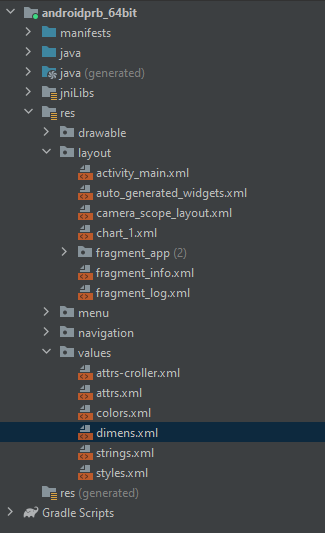
\includegraphics[scale=0.5]{android_apps/android_f1.png}
\end{figure}

dentro del archivo \texttt{dimens.xml} se encuentran las siguientes declaraciones: \newpage

\begin{verbatim}
<resources>
    <!-- Default screen margins, per the Android Design guidelines. -->
    <dimen name="activity_horizontal_margin">16dp</dimen>
    <dimen name="activity_vertical_margin">16dp</dimen>
    <dimen name="fab_margin">16dp</dimen>
    <dimen 
        name="appbar_padding">8dp</dimen>
    <dimen 
        name="appbar_padding_top">8dp</dimen>
    <dimen name="appname_bar_height">30dp</dimen>
    <dimen name="appname_textsize">20dp</dimen>
    <dimen name="info_cardview_margin">10dp</dimen>
    <dimen name="info_linear_padding">20dp</dimen>
    <dimen name="divider_height">2dp</dimen>
    <dimen name="info_sectiondata_paddingtop">5dp</dimen>
    <dimen name="info_sectiontitle_paddingbottom">10dp</dimen>
    <dimen name="uimarginbottom">8dp</dimen>
</resources>
\end{verbatim}

Y dentro de los \texttt{views} se pueden referir a estas variables mediante la siguiente forma: \\

\texttt{android:layout\_height="@dimen/appname\_bar\_height"}
% \chapter{Circuitos eléctricos}


\section{Teoremas de circuitos}


Una de las desventajas del análisis de circuitos mediante las eyes de Kirchhoff es que implica en gran medida circuitos complejos y tesiosos calculos. Se han desarrollado algunos teoremas para enfrentar esta compejidad. Entre estos teoremas están el teorema de Thevenin y el teorema de Norton como estos teoremas se aplican a circuitos lineales, primero se expondrá el concepto de lonealidad en los circuitos. También se expondrá el concepto de transformación de fuentes y máxima transferencia de potencia.

\subsection{Linealidad}



\subsection{Superposición}



\subsection{Transformación de fuentes}


\subsection{Teorema de Thevenin}

Teniendo en cuenta que la carga de un circuito en general es variable, el circuito entero debe vovler a analizarse. El teorema de thevenin evita este problema; proporciona una técnica mediante la cual la parte fija del circuito de reemplaza por un circuito equivalente. 

\begin{figure}[H]
    \centering
    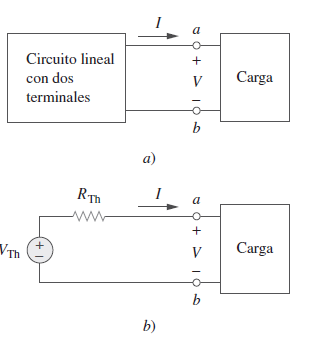
\includegraphics[scale=0.5]{Elect_circ/fig_circequiv.png}
\end{figure}

El teorema de Thevenin establece que un circuito lineal de dos terminales puede reemplazarse por un vurvuito equivalente que consta de una fuente de tension $V_{th}$ en seriie cin una resistentia $R_{th}$, donde $V_{th}$ es la tensión del circuito abierto en las terminales y $R_{th}$ es la entrada o la resistencia equivalente en las terminales cuando las fuentes están apagadas.

Para aplicar esta idea en el calculo de la resistencia de Thevenin se deben considerar dos casos

\begin{enumerate}
    \item Si la red no tiene fguentes dependientes, se apagan todas las fuentes independientes. $R_{th}$ es la resistencia equivalente de entrada que aparece entre las terminales.
    \item Si kla red tiene fuentes dependientes, se deben apagar todas las fuentes independientes, y se debe aplicar una tensión de prueba en las terminales. Se deberá medir la corriente resultante del circuito de prueba y la resistencia thevenin será $T_{th} = \frac{v_o}{i_o}$. De manera alternativa se puede aplicar una fuente de corriente de prueba y de manera análoga se determina la resistencia thévenin midiendo la tensión resultante en las terminales y dividiendo por la corriente de prueba.
\end{enumerate}

para el circuito equivalente de Thevenin 

\begin{figure}[H]
    \centering
    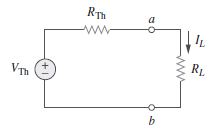
\includegraphics{Elect_circ/circ_f2.png}
\end{figure}

Se puede determinar la corriente $I_L$:

\begin{eqnarray*}
I_L = \frac{V_{Th}}{R_{Th}+R_L} \\
V_L = V_{Th} \frac{R_{L}}{R_{Th}+R_L}
\end{eqnarray*}

\subsection{Teorema de Norton}

El teorema de Norton establece que un circuito lineal de dos terminares puede reemplazarse por un curcuito equivalente que consta de una fuente de corriente $I_N$ en paralelo con un resistor $R_N$, sonde $I_n$ es la corriente de corto circuito a través de las terminales y $R_N$ es la resistencia de entrada o la resistencia equivalente en las terminales cuando las fuentes independientes están apagadas. \\

la resistencia de Norton y la resistencia de Thevenin son equivalentes. 

\begin{equation*}
R_n = R_{Tn}
\end{equation*}

Y por la transfornacion de fuentes:

\begin{equation*}
I_N = \frac{V{Th}}{R_{Th}}
\end{equation*}

\subsection{Máxima transferencia de potencia} \label{max_transf_pot}

\begin{figure}[H]
    \centering
    \includegraphics{Elect_circ/circ_f3.png}
\end{figure}

Para la figura anterior, podemos determinar la potencia que consume la carga $R_L$, esta potencia es

\begin{equation*}
p = i^2 R_L = \left( \frac{V_{Th}}{R_{Th}+R_L} \right)^2 R_L
\end{equation*}

Indica una función de $R_L$ que si se analiza se puede determinar que es nula en $R_L=0$ y $R_L \to \infty$, y tiene un máximo. Dicho máximo se puede determinar derivando la función e igualando a cero:

\begin{eqnarray*}
\frac{d p}{d R_L} = V_{Th}^{2} \left(  \frac{R_{Th}+R_L - 2R_L}{(R_{Th}+R_L)^3} \right) = 0 \\
R_l = R_{Th}
\end{eqnarray*}

Lo cual indica que para la máxima transferencia de potencia a la carga, esta debe tener una resistencia igual a la resistencia Thevenin del circuito. Si se cumple esto, esta potencia estará dada por

\begin{equation*}
p_{\text{max}} = \frac{V_{Th}^2}{4 R_{Th}}
\end{equation*}





\section{Potencia de ca}


La potencia es la cantidad más relevante en todos los sistemas de suministro de neregía. Cada máquina electrica tiene un valor de potencdia nominal que indica cuánta potencia requiere la misma. En principop se definene la potencia instantánea y la potencia promedio. después se presentarán otros conceptos de potendcia.


\subsection{Potencias instantánea y promedio} 
La potencia instantánea absorbida or un elemento de ircuito dse define como la multiplicación de la tensión y la corriente instantáneas.

\begin{equation*}
    p(t) = v(t) i(t)
\end{equation*}

Se puede concebir como la potencia absorbida por ele elemento un instante específico. Las cantidades instantánteas se suelen denotar con letras minúsculas. Su unidad de medida es el vatio (W). \\

Como ejemplo sea un circuito en cuyas dos terminales arbitrarias se mide la tensión y la corriente y estas son

\begin{eqnarray*}
    v(t) = V_m \cos (\omega t + \theta_v) \\
    I(t) = I_m \cos (\omega t + \theta_i)
\end{eqnarray*}

La potencia instantánea absorbida por el circuito es 

\begin{equation*}
p(t) = v(t) i(t) = V_m I_m \cos (\omega t + \theta_v) \cos (\omega t + \theta_i)
\end{equation*}

Aplicando la identidad trigonométrica 

\begin{equation*}
\cos A \cos B = \frac{1}{2} [\cos(A-B) + \cos (A+B)]
\end{equation*}

Se expresa la potencia instantánea de la siguiente forma

\begin{equation*}
p(t) = \frac{1}{2} V_m I_m \cos (\theta_v - \theta_i) + \frac{1}{2}V:m I_m \cos (2 \omega t + \theta_v + \theta_i)
\end{equation*}

Esto indica que la potencia instntanea tiene dos partes, una de las cuales es independiente ddel tiempo. Su valor depende de la diferencia de las fases de la tensión y de cirriente. La segunda parte es una fución sinussoidal cuya frecuencia es el doble de la frecuencia de la tensión y corriente.

La potencia instantánea es dif´´oicil de medir, por tanto aparece la potencia promedio. El watímetro que es el instrumento de medición de potencia, mide la potencia promedio. Esta potencia está dada por

\begin{equation*}
P = \frac{1}{T} \int_0^T p(t) dt
\end{equation*}

Aplicando la integral a la potencia sinusoidal de antes tenemos 

\begin{eqnarray*}
P = \frac{1}{2}V_m I_m \cos(\theta_v - \theta_i) \frac{1}{T} \int_0^T dt +  \frac{1}{2}V_m I_m \frac{1}{T} \int_0^T \cos (2 \omega t + \theta_v + \theta_i) dt 
\end{eqnarray*}

Esta expresión se simplifica a 

\begin{equation*}
P = \frac{1}{2} V_m I_m \cos (\theta_v - \theta_i)
\end{equation*}

Teniendo en cuenta la notación fasorial $\mathbf{V}=V_m \angle \theta_v$ e $\mathbf{I}=I_m\angle \theta_i$ podemos partir de que

\begin{eqnarray*}
\frac{1}{2} \mathbf{V} \mathbf{I}^{*} &=& \frac{1}{2}V_m I_m \angle (\theta_v - \theta_i) \\
 &=& \frac{1}{2}V_m I_m \left( \cos (\theta_v - \theta_i) + j \sin (\theta_v - \theta_i) \right)
\end{eqnarray*}

Por tanto podemos denotar de manera fasorial la potencia promedio así

\begin{equation*}
P = \frac{1}{2} \mathrm{Re}\{ \mathbf{VI^{*}} \} =  \frac{1}{2}V_m I_m \cos (\theta_v - \theta_i)
\end{equation*}

La potencia promedio disipada en una resistencia será

\begin{equation*}
P = \frac{1}{2} |\mathbf{I}|^2 R
\end{equation*}

Observe que cuando el desfase entre tensión y corriente es nulo, la potencia es máxima; indica un circuito puramente resistivo, si el desfase es máximo, es decir $90$ grados, la potencia promedio es nula y el circuito es puramente reactivo. 

\subsection{Máxima transferencia de potencia promedio}

En la sección \ref{max_transf_pot} se determinó cómo se maximiza la potencia entregada por una circuito a una carga mediante su equivalente de Thevenin. Se determino que la máxima transferencia se logra cuando la resistencia de  carga es igual a la resistencia de Thevenin.

Para los circuitos de corriente alterna, considere 

\begin{figure}[H]
    \centering
    \includegraphics{Elect_circ/pot_f1.png}
\end{figure}

Las impedancias de thevenin y de carga pueden ser en forma triangular

\begin{eqnarray*}
\mathbf{Z}_{Th} = R_{Th} + j X_{Th} \\
\mathbf{Z}_{L} = R_{L} + j X_{L}
\end{eqnarray*}

La corriente que fluye por la carga será

\begin{equation*}
\mathbf{I} = \frac{\mathbf{V}_{Th}}{\mathbf{Z}_{Th} + \mathbf{Z}_L} = \frac{\mathbf{V}_{Th}}{ (R_{Th} + j X_{Th}) + (R_L + jX_L) }
\end{equation*}

Para este caso, la potencia promedio suministrada a la carga en este caso será

\begin{equation*}
P = \frac{1}{2}|\mathbf{I}|^2 R = \frac{|\mathbf{V}_{Th}|^2R_L/2}{(R_{Th} + R_L )^2 + (X_{Th} + X_L)^2}
\end{equation*}

El objetivo es ajustar los parámetros de carga $R_L$ y $X_L$ para que la potencia sea máxima. Para ello derivamos $P$ con respecto a $R_L$ y a $X_L$ e igualamos acero

\begin{eqnarray*}
\frac{\partial P }{\partial  X_L} = -\frac{|\mathbf{V}_{Th}|^2 R_L (X_{Th} + X_L)}{\left[ (R_{Th} + R_L)^2 + (X_{Th} + X_L)^2\right]^2} \\
\frac{\partial P }{\partial  R_L} = \frac{|\mathbf{V}_{Th}|^2 \left[(R_{Th} + R_L)^2 + (X_{Th} + X_L)^2 - 2R_L(R_{Th} + R_L)   \right]}{2 \left[ (R_{Th} + R_L)^2 + (X_{Th} + X_L)^2\right]^2}
\end{eqnarray*}


La solucion a este sistema de ecuaciones deja:

\begin{eqnarray*}
X_L = -X_{Th} \\
T_L = R_{Th}
\end{eqnarray*}

De manera que en conclusión, la impedancia de carga que maximiza la absorción de potencia de un circuito de CA es 

\begin{equation*}
\mathbf{Z}_L = \mathbf{Z}_{Th}^{*}
\end{equation*}

El complejo conjugado de la impedancia equivalente de Thevenin.

Esta potencia m+axima es 

\begin{equation*}
P_{\text{max}} = \frac{|\mathbf{V}_{Th}|^2}{8 T_{Th}}
\end{equation*}

En la situación en que la carga es puramente real, la condición para la máxima transferencia de potencia promedio deriva de 

\begin{equation*}
R_L = \sqrt{R_{Th}^2 + (X_{Th} + X_L)^2}
\end{equation*}

fijando $X_L=0$,

\begin{equation*}
R_L = \sqrt{R_{Th}^2 + (X_{Th})^2} = |\mathbf{Z}_{Th}|
\end{equation*}

\subsection{Valor efizar o RMS}

La idea del valor eficaz surge de la necesidad de medir la eficacia de una fuente de tensión o de corriente en el suministro de potencia a una carga resistiva.

El valor eficaz de una corriente periódica es la corriente de continua que suministraría la misma potencia promedio a una resistencia que la corriente periódica

\begin{figure}[H]
    \centering
    \includegraphics{Elect_circ/pot_f2.png}
\end{figure}

La potencia consumida por $R$ en el circuito AC es

\begin{equation*}
P=\frac{R}{T}\int_{0}^T i^2 dt
\end{equation*}

Mientras que la potencia en el circuito DC es

\begin{equation*}
P = I_{RMS}^2 R
\end{equation*}

Igualando estas dos potencial obtenemos que 

\begin{equation*}
I_{RMS} = \sqrt{\frac{1}{T}\int_0^T i^2 dt}
\end{equation*}

De la misma forma para la tensión eficaz, y para cualquier señal o función periódica en general. Aplicando este operador a una función sinusoidal se obtiene que el valor RMS es

\begin{equation*}
V_{RMS} = \frac{V_m}{\sqrt{2}} 
\end{equation*}

La potencia promedio se puede expresar en términos de tensión y corriente eficaces

\begin{eqnarray*}
p &=& \frac{1}{2}V_m I_m \cos (\theta_v - \theta_i) \\
&=& V_{RMS} I_{RMS} \cos (\theta_v - \theta_i) 
\end{eqnarray*}

Del mismo modo, la potencia promedio absorbida por una resistencia es

\begin{equation*}
P = \frac{V_{RMS}^2}{R}
\end{equation*}

\subsection{Potencia aparente y factor de potencia}

Como se vio anteriormente, podemos expresar la potencia promedio dadad dos señales de tensión y corriente de la siguiente forma

\begin{equation*}
P = V_{\textbf{RMS}} I_{\textbf{RMS}} \cos  (\theta_v - \theta_i) 
\end{equation*}

Sea $S=V_{\textbf{RMS}} I_{\textbf{RMS}}$, por tanto queda la anterior ecuación

\begin{equation*}
P = S  \cos  (\theta_v - \theta_i)
\end{equation*}

Se define $S$ como la \textbf{potencia aparente}, y el factor $ \cos  (\theta_v - \theta_i)$ es el \textbf{factor de potencia}.

La potencia aparente se llama así porque aparentemente la potencia debería ser el producto entre la tensión y la cdorriente, por analogia con los circuitos resistivos DC. Esta potencia se mide en volti-amperios (VA) para distinguirla de la potencia promedio o \textbf{real} medida en (W). \\

El ángulo $ (\theta_v - \theta_i)$ se conoce como el ángulo de factor de potencia. Si tomamos en cuenta el hecho de que en un elemento tenemos tensión $V_m \angle \theta_v$ y una corriente igual a $I_m \angle \theta_i$, la impedancia de dicho elemento es

\begin{equation*}
\mathbf{Z}=\frac{\mathbf{V}}{\mathbf{I}} = \frac{V_m \angle \theta_v}{I_m \angle \theta_i} = \frac{V_m}{I_m} \angle (\theta_v - \theta_i)
\end{equation*}

Por tanto el factor de potencia es el coseno del ángulo de la impedancia, alternativamente:

\begin{equation*}
\mathbf{Z}=\frac{V_\textbf{RMS}}{I_\textbf{RMS}} \angle (\theta_v - \theta_i)
\end{equation*}

El factor de potencia es el coseno del ángulo de desfase entre la tensión y la corriente, también es el coseno del ángulo de la impedancia de la carga. \\

Si el ángulo de desfase va desde -90 hasta 90, su coseno varía entre 0 y 1, cuando el factor de potencia es diferente de 1 se dice que está adelantado o atrasado. Un factor de potencia adelantado significa que la corriente se adelanta a la tensión, lo cual indica una carga caácitiva. Un factor de potencia atrasado significa que la corriente se atrasa de la tensión, lo cual implica una carga inductiva.

\begin{eqnarray*}
\mathbf{Z} = 25-j38.5 \Omega \text{denota un adelanto de fase, por tanto una carga capacitiva} \\
\mathbf{Z} = 25+j74 \Omega \text{denota un atraso de fase, por tanto una carga inductiva}
\end{eqnarray*}

Recordemos que 

\begin{eqnarray*}
\mathbf{Z} = R + j X_L \text{ o } R-jX_C \\
X_C = \frac{1}{\omega C} = \frac{1}{2 \pi f C}\\
X_L = \omega L = 2 \pi f L
\end{eqnarray*}

\subsection{Potencia compleja}

A lo largo de los años se han invertido considerables esfuerzos para expresar las relaciones de potencia en la forma más sencilla posible. Los ingenieros del área de potencia han acuñado el término potencia compleja, que emplean para hallar el efecto total de cargas en paralelo. La potencia compleja es importante en el análisis de potencia a causa de que contiene toda la información correspondiente a la potencia recibida por una carga dada. \\

Sea una carga $\mathbf{Z}$ cuya corriente es $\mathbf{I} = I_m \angle \theta_i$ y tensión $\mathbf{V}=V_m \angle \theta_v$. La potencia compleja $\mathbf{S}$ recibida por la carga AC es el producto de la tensión por el conjugado de la corriente

\begin{equation*}
\mathbf{S} = \frac{1}{2}\mathbf{V} \mathbf{I}^* = \mathbf{V}_{\text{RMS}} \mathbf{I}_{\text{RMS}}^{*} = \frac{V_\text{RMS}^2}{\mathbf{Z}^*}
\end{equation*}

donde 
\begin{eqnarray*}
\mathbf{V}_{\text{RMS}} = \frac{\mathbf{V}}{\sqrt{2}} \\
\mathbf{I}_{\text{RMS}} = \frac{\mathbf{I}}{\sqrt{2}}
\end{eqnarray*}

Veamos que la potencia compleja es

\begin{equation*}
\mathbf{S} = P + j Q
\end{equation*}

donde

\begin{eqnarray*}
P = \text{Re}\{ \mathbf{S} \} = I_\text{RMS}^2 R \\
Q = \text{Im} \{ \mathbf{S} \} = I_\textbf{RMS}^2 X
\end{eqnarray*}

Recordemos: \\

\textbf{P es la potencia promedio o real, Q es la potencia reactiva y $|\mathbf{S}|$ es la potencia aparente}

\begin{figure}[H]
    \centering
    \includegraphics{Elect_circ/pot_f3.png}
\end{figure}

\subsection{Corrección del factor de potencia}

La mayoría de las cargas domésticas (como lavadoras, neveras, aire acondicionado, etc) y de las cargas industriales (como motores de inducción) son inductivasy operan con un factor de potencia bajo y atrasado. Aunque la naturaleza inductiva de la carga no puede modificarse, es posible incrementar su factor de potencia. \\

Dado que la mayoría de las cargas son inductivas, el factor de potencia de una carga se mejora o se corrige al instalar deliberadamente un capacitor en paralelo con la carga. El efecto de añadir el capacitor puede ilustrarse cin el truángulo de potencia o el diagrama fasorial de las corrientes implicadas.\\

La corrección del factor de potencia puede examinarse desde el siguiente punto de vista: considere un triángulo de potencia 

\begin{figure}[H]
    \centering
    \includegraphics{Elect_circ/pot_f4.png}
\end{figure}

Si la carga inductiva original tiene la potencia aparente $S_1$ entonces

\begin{eqnarray*}
P = S_1 \cos \theta_1 \\
Q_1 = S_1 \sin \theta_1 = P \tan \theta_1
\end{eqnarray*}

Si se desea incrementar el factor de potencia de $\theta_1$ a $\theta_2$ sin alterar la potencia real ($P = S_2 \cos \theta_2$), la nueva potencia reactiva es 

\begin{equation*}
Q_2 = P \tan \theta_2
\end{equation*}

La reducción de la potencia reactiva es causada por el capacitor en derivación

\begin{equation*}
Q_c = Q_1 - Q_2 = P(\tan \theta_1 - \tan \theta_2)
\end{equation*}

pero como sabemos 

\begin{equation*}
Q_C = \frac{V_\text{RMS}^2}{X_C} = V_\text{RMS}^2 \omega C
\end{equation*}

\begin{equation*}
C = \frac{Q_C}{V_\text{RMS}^2 \ \omega} = \frac{P (\tan \theta_1 - \tan \theta_2)}{\omega V_\text{RMS}^2}
\end{equation*}

De manera análoga, para atrasar un factor de potencia adelantado, se debe conectar un inductor a la carga, y el valor de este inductor estará dado por

\begin{equation*}
L \frac{V_\text{RMS}^2}{\omega Q_L}
\end{equation*}


\section{Circuitos trifásicos}

Un circuito trifásico balanceado consta de tres fuentes de tensión con un desfase de 120 grados entre sí y que pueden estar conectados de las siguientes maneras

\begin{figure}
    \centering
    \includegraphics{Elect_circ/trif_f1.png}
\end{figure}

La primera configuración se llama estrella y tiene 4 terminales, una de las cuales se considera punto neutral. Las tensiones $\mathbf{V}_{an},\mathbf{V}_{bn},\mathbf{V}_{cn}$ se denominan tensiones de fase, y estas tensiones se dice que están balanceadas si tienen la misma frecuencia, amplitud y están desfasadas 120 gradeos entre sí. Esto implica que

\begin{equation*}
\mathbf{V}_{an} + \mathbf{V}_{bn} + \mathbf{V}_{cn} = 0
\end{equation*}

\begin{equation*}
|\mathbf{V}_{an}|=|\mathbf{V}_{bn}|=|\mathbf{V}_{cn}|
\end{equation*}

Existen dos formas en las que están configuradas las fases:

\begin{eqnarray*}
\mathbf{V}_{an} = V_P \angle 0^{o}  \\
\mathbf{V}_{bn} = V_P \angle -120^{o} \\
\mathbf{V}_{cn} = V_P \angle 120^{o}
\end{eqnarray*}

\begin{eqnarray*}
\mathbf{V}_{an} = V_P \angle 0^{o} \\
\mathbf{V}_{cn} = V_P \angle  -120^{o} \\
\mathbf{V}_{bn} = V_P \angle  120^{o}
\end{eqnarray*}

La primera se conoce como secuencia abc o positiva. La segunda secuencia se denomina acb o negativa.


Al igual que con el generador, las cargas también se pueden conectar en estrella o en fase. En una carga balanceada las tres impedancias tiene el mismo valor. En una carga balanceada en estrella

\begin{equation*}
\mathbf{Z}_1 = \mathbf{Z}_2 = \mathbf{Z}_3 = \mathbf{Z}_Y
\end{equation*}

en una carga balanceada en delta,

\begin{equation*}
\mathbf{Z}_a = \mathbf{Z}_b = \mathbf{Z}_c = \mathbf{Z}_{\Delta}
\end{equation*}

La relación entre ambos tipo de impedancia es

\begin{eqnarray*}
\mathbf{Z}_{\Delta} = 3 \mathbf{Z}_Y
\end{eqnarray*}

\subsection{Conexión estrella-estrella balanceada}

Considere una fuente trifásica en estrella conectada con una carga estrella balanceada, si se tiene en cuenta la impadancia interna o impedancia de fuente y la impedancia de línea, se puede considerar una impedancia de carga como la suma (serie) de impedancia de carga, línea y fuente.

Es evidente que se puede realizar la suma fasorial de las tensiones de fase para determinar los valores de tensiones de línea:

\begin{eqnarray*}
\mathbf{V}_{bc} = \mathbf{V}_{an} - \mathbf{V}_{bn} = \sqrt{3} V_p \angle 30^{o} \\
\mathbf{V}_{bc} = \mathbf{V}_{an} - \mathbf{V}_{bn} = \sqrt{3} V_p \angle 30^{o} \\
\mathbf{V}_{bc} = \mathbf{V}_{an} - \mathbf{V}_{bn} = \sqrt{3} V_p \angle 30^{o}
\end{eqnarray*}

La magnitud de las tensiones de línea es igual a $\sqrt{3}$ veces la magnitud de las tensiones de fase.

\subsection{Potencia en un sistema balanceado}

Considere ahora la potencia en un sistema trif+asico balanceado. Se comenzará examinando la potencia instantánea absorbida por la carga. Esto requiere que el análisis se realice en el dominio temporal. En na carga conectada en Y, las tensiones de fase son

\begin{eqnarray*}
v_{an} &=& \sqrt{2} V_P \cos \omega t \\
v_{bn} &=& \sqrt{2} V_P \cos (\omega t -120 ) \\
v_{cn} &=& \sqrt{2} V_P \cos (\omega t +120 )
\end{eqnarray*}

El factor $\sqrt{2}$ es necesario porque $V_P$ se definió como el valor RMS. $\mathbf{Z}_Y = Z \angle \theta$, las corrientes de fase se atrasan respecto a las tensiones de fase respectivas en $\theta$, es decir

\begin{eqnarray*}
i_a &=& \sqrt{2} I_P \cos (\omega t - \theta) \\
i_b &=& \sqrt{2} I_P \cos (\omega t - \theta - 120) \\
i_c &=& \sqrt{2} I_P \cos (\omega t - \theta + 120)
\end{eqnarray*}

La potencia instantánea total en la carga es la suma de las potencias instantáneas en las tres fases

\begin{equation*}
p = p_a + p_b + p_c = v_{AN}i_a + v_{BN} i_b + v_{CN} i_c
\end{equation*}

\begin{eqnarray*}
p &=& V_p I_p \left[ 3 \cos \theta + \cos (2 \omega t \theta) + \cos (2 \omega t - \theta - 240) + \cos(2 \omega t - \theta + 240) \right] \\
  & & \textbf{donde } \alpha = 2 \omega t - \theta \\
&=& V_pI_p \left[ 3 \cos \theta + \cos \alpha +2 \left( -\frac{1}{2} \right) \cos \alpha \right] \\
&=& 3V_pI_p \cos \theta
\end{eqnarray*}

note cómo la potencia instantánea es independiente del tiempo. Esto es verdad ya sea que la carga esté conectada en $Y$ o en $\Delta$. \\

La potencia promedio por fase es igual a $p/3$

\begin{equation*}
P_P = V_p I_p \cos \theta
\end{equation*}
 Y las potencias reactiva y aparente son 

\begin{eqnarray*}
Q_p = V_p I_p \sin \theta \\
S_p = V_p I_p
\end{eqnarray*}

  Finalmente la potencia compleja es

\begin{equation*}
\mathbf{S}_p = P_p + j Q_p = \mathbf{V}_p \mathbf{I}_p^{*}
\end{equation*}

La potencia total es la suma de las potencias promedio, así

\begin{equation*}
P = P_a + P_b + P_c = 3 P_p = 3 V_p I_p \cos \theta = \sqrt{3}V_L I_L \cos \theta
\end{equation*}

Tenga en cuenta que en estrella $I_P = I_L$, pero $V_L = \sqrt{3}V_P$ mientras que en $\Delta$ $V_L = V_P$ pero $I_L = \sqrt{3}I_P$. Así esta ecuación anterior se aplica en ambas configuraciones. Del mismo modo la potencia reactiva total es 

\begin{equation*}
Q = 3V_P I_P \sin \theta = 3 Q_P = \sqrt{3} V_L I_L \sin \theta 
\end{equation*}

 Y la potencia completa total es

\begin{eqnarray*}
\mathbf{S} &=& 3\mathbf{S}_p = 3 \mathbf{V}_P \mathbf{I}_P^{*} = 3I_P^2\mathbf{Z}_P = \frac{3 V_p^2}{\mathbf{Z}_P^{*}} \\
&=& P + j Q = \sqrt{3} V_L I_L \angle \theta
\end{eqnarray*}

Recordemos que estos valores son RMS y que el ángulo $\theta$ es el ángulo de la impedancia de la carga trifásica o de desfase entre tensión y corriente.

% \chapter{Circuitos electrónicos}

\section{Amplificadores operacionales}

\subsection{Amplificadores diferenciales}

\subsubsection*{El amplificador de instrumentación}

Alguna configuración de amplificador diferencial tiene el inconveniente de que si resistencia de entrada es muy bajita, además de que es complicado configurar una ganancia. El siguiente circuito resuelve el problema:

\begin{figure}[H]
    \centering
    \includegraphics[scale=0.6]{Electronica/electronic_f1.png}
\end{figure}

La salida de la señal está dada por 

\begin{equation*}
\left( \frac{R_4}{R_3} \right) \left( \frac{R_1 + R_2}{R_1} \right) \left( v_{I2} - v_{I1} \right)
\end{equation*}

note que las salidas de las primeras etapas están dadas por $R_1$ y $R_2$, luego se amplifica por $R_3$ y $R_4$. 

Vemos de este circuito dos principales desventajas 

\begin{enumerate}
    \item Los dos amplificadores de la primera etapa deben estar perfectamente sincronizados.
    \item Para variar o configurar la ganancia diferencial, es necesario variar simultáneamente dos resistencias; en la práctica es muy complicado sincronizar el valor de dos resistencia de manera perfecta.
\end{enumerate}

\section{Breve resumen de semiconductores}

En esta sección se tratará muy brevemente y por encima la física y las propiedades de los semiconductores. Todo para introducir los conocimientos necesarios para abordar la física de los diodos y los transistores.

\subsection{Semiconductores intrínsecos}

Como su nombre indica, los semiconductores son materiales cuya conductividad se encuentra entre la de los conductores, como el cobre,, y los aislantes, como el vidrio. Hay dos tipos de semiconductores: semiconductores de un solo elemento como el germanio y el silicio, que se encuentran en el grupo VI de la tabla periódica; y semiconductores compuestos como el arseniuro de galio, que se forman combinando elementos de los grupos III y V o los grupos II y IV. Los semiconductores compuestos son útiles en aplicaciones especiales de circuitos electrónicos, así como en aplicaciones que implican luz, como los diodos emisores de luz. De los dos semiconductores elementales, el germanio se utilizó en la fabricación de los primeros transistores (finales de la década de 1940, principios de la década de 1950). Sin embargo, fue rápidamente reemplazado por el silicio, en el cual se basa casi completamente la tecnología de circuitos integrados de hoy en día. Por esta razón, trataremos principalmente con dispositivos de silicio a lo largo de este libro. Un átomo de silicio tiene cuatro electrones de valencia, por lo que necesita otros cuatro para completar su capa más externa. Esto se logra compartiendo uno de sus electrones de valencia con cada uno de sus cuatro átomos vecinos. Cada par de electrones compartidos forma un enlace covalente. El resultado es que un cristal de silicio puro o intrínseco tiene una estructura de retícula regular, donde los átomos se mantienen en su posición por los enlaces covalentes. \\

A temperaturas suficientemente bajas, cercanas al cero absoluto (0 K), todos los enlaces covalentes permanecen intactos y no hay electrones disponibles para conducir la corriente eléctrica. Por lo tanto, el cristal de silicio intrínseco actúa como un aislante a estas temperaturas.
Sin embargo, a temperatura ambiente, existe suficiente energía térmica para romper algunos de los enlaces covalentes, un proceso conocido como generación térmica. Cuando se rompe un enlace covalente, se libera un electrón, que puede alejarse de su átomo original y conducir la corriente eléctrica si se aplica un campo eléctrico al cristal.
Al alejarse, el electrón deja detrás una carga positiva neta, a la que puede ser atraído un electrón de un átomo vecino, dejando a su vez un "hueco" en su lugar. Este proceso puede repetirse, creando una especie de portador de carga positiva, o hueco, que se mueve por la estructura del cristal de silicio y también puede conducir la corriente eléctrica.
A medida que aumenta la temperatura, se rompen más enlaces covalentes y se generan más pares de electrones y huecos. El incremento en el número de electrones libres y huecos resulta en un aumento en la conductividad del silicio.

La generación térmica resulta en electrones libres y huecos en igual número y, por lo tanto, en igual concentración, donde la concentración se refiere al número de portadores de carga por unidad de volumen (cm3). Los electrones libres y los huecos se mueven aleatoriamente a través de la estructura cristalina del silicio, y en el proceso, algunos electrones pueden llenar algunos de los huecos. Este proceso, llamado recombinación, resulta en la desaparición de electrones libres y huecos. La tasa de recombinación es proporcional al número de electrones libres y huecos, que a su vez está determinada por la tasa de generación térmica. Esta última es una función fuerte de la temperatura. En equilibrio térmico, la tasa de recombinación es igual a la tasa de generación, y se puede concluir que la concentración de electrones libres n es igual a la concentración de huecos p.

\begin{equation*}
n = p = n_i
\end{equation*}

donde $n_i$ denota el número de electrones libres y huecos en una unidad de volumen ($cm^3$) de silicio intrínseco a una temperatura dada. Los resultados de la física de semiconductores dan $n_i$ como

\begin{equation*}
n_i = BT^{3/2} e^{\frac{-E_g}{2kT}}
\end{equation*}

donde B es un parámetro dependiente del material que es $7.3 \ 10^15 cm^{-3}K^{-3/2}$ para el silicio; $T$ es la temperatura en K; $E_g$, un parámetro conocido como la energía de Fermi, es de $1.12 Ev$ para el silicio; y $k$ es la constante de Boltzmann ($8.62 \ 10^-5 eV/K$). 
Es interesante saber que la energía de la banda prohibida $E_g$ es la energía mínima requerida para romper un enlace covalente y, por lo tanto, generar un par de electrones-huecos.

Finalmente, es útil conocer la relación de portadores y la concentración 

\begin{equation*}
p \ n = n_i^2 
\end{equation*}

Para el silicio a temperatura ambiente, $n_i \approx 1.5 \ 10^{10} cm^{-3}$


\subsection{Semiconductores dopados}

El cristal de silicio intrínseco que se describió anteriormente tiene igual concentración de electrones libres y huecos, generados por la generación térmica. Sin embargo, estas concentraciones son demasiado pequeñas para que el silicio conduzca una corriente apreciable a temperatura ambiente. Además, las concentraciones de portadores y, por ende, la conductividad, son funciones fuertes de la temperatura, lo cual no es una propiedad deseable en un dispositivo electrónico. Afortunadamente, se desarrolló un método para cambiar la concentración de portadores en un cristal semiconductor de forma sustancial y controlada. Este proceso se conoce como dopado, y el silicio resultante se conoce como silicio dopado.

El dopado implica la introducción de átomos de impurezas en el cristal de silicio en cantidades suficientes para aumentar de forma considerable la concentración de electrones libres o huecos, pero con poco o ningún cambio en las propiedades cristalinas del silicio. Para aumentar la concentración de electrones libres, se dopa el silicio con un elemento con una valencia de 5, como el fósforo, y el silicio dopado resultante se conoce como tipo n. Para aumentar la concentración de huecos, se dopa el silicio con un elemento con una valencia de 3, como el boro, y el silicio dopado resultante se conoce como tipo p.

Un ejemplo de esto es un cristal de silicio dopado con fósforo. Los átomos de fósforo reemplazan a algunos de los átomos de silicio en la estructura cristalina. Como el átomo de fósforo tiene cinco electrones en su capa externa, cuatro de estos electrones forman enlaces covalentes con los átomos vecinos, y el quinto electrón se convierte en un electrón libre. Así, cada átomo de fósforo dona un electrón libre al cristal de silicio, y la impureza de fósforo se llama donante. Sin embargo, este proceso no genera huecos. La carga positiva neta asociada con el átomo de fósforo es una carga ligada que no se mueve a través del cristal.

Si la concentración de átomos donantes es ND, donde ND es usualmente mucho mayor que ni, la concentración de electrones libres en el silicio de tipo n será

\begin{equation*}
n_n \approx N_D
\end{equation*}

De la ecuación de portadores se tiene que 

\begin{equation*}
p_n = \frac{n_i^2}{N_D}
\end{equation*}

Así, $p_n$ tendrá la misma dependencia de la temperatura que $n_i^2$. Finalmente, debemos notar que en el silicio de tipo n, la concentración de electrones libres $n_n$ será mucho mayor que la de los huecos. Por lo tanto, se dice que los electrones son los portadores de carga mayoritarios y los huecos los portadores de carga minoritarios en el silicio de tipo n.

Para semiconductores tipo $p$ se tiene concentraciones $N_A \gg n_i$

\begin{equation*}
p_p \approx N_A
\end{equation*}

\begin{equation*}
p_p n_p = n_i^2
\end{equation*}

\begin{equation*}
n_p \approx \frac{n_i^2}{N_A}
\end{equation*}

\subsection{Flujo de corriente en el semiconductor}

Hay dos mecanismos para el movimiento de los portadores de carga: por arrastre y por difusión

\subsubsection{Corriente de arrastre}

cuando hay un campo eléctrico $E$ aplicado en el cristal semiconductor, los huecos son acelerados en la dirección del campo, y los electrones libres en la dirección contraria. Los huecos adquieren entonces una velocidad de arrastre ada por 

\begin{equation*}
v_{p-drift} = \mu_p E
\end{equation*}

Donde el término $\mu_p$ se denomina movilidad de huecos.  Representa la facilidad con la que los huecos se mueven a través del cristal. La movilidad de huecos para los cristales semiconductores de silicio es 

\begin{equation*}
\mu_p = 480 \ \frac{\text{cm}^2}{\text{V s}}
\end{equation*}

La movilidad de los electrones es por su parte 

\begin{equation*}
v_{n-drift} = -\mu_n E
\end{equation*}

\begin{equation*}
\mu_n = 1350 \ \frac{\text{cm}^2}{\text{V s}}
\end{equation*}

\begin{figure}[H]
    \centering
    \includegraphics[scale=0.6]{Electronica/semiconductor_f1.png}
\end{figure}

Volviendo al barra de silicio monocristalino mostrada en la última imagen, sea p la concentración de huecos y la de electrones libres sea n. Queremos calcular el componente de corriente debido al flujo de huecos. Consideremos un plano perpendicular a la dirección x. En un segundo, la carga del hueco que cruza ese plano será de ($A q p v_{p-drift}$) culombios, donde A es el área transversal de la barra de silicio y q es la magnitud de la carga del electrón. Esto debe ser el componente del hueco de la corriente de deriva que fluye a través de la barra.

\begin{eqnarray*}
I_P &=& A q p v_{p-drift} \\
I_P &=& A q p \mu_p E
\end{eqnarray*}

La densidad de corriente será entonces

\begin{equation*}
J_p =\frac{I_p}{A} = q p \mu_p E
\end{equation*}

El componente de corriente debido a la deriva de los electrones libres se puede encontrar de manera similar. Sin embargo, debemos notar que los electrones que derivan de derecha a izquierda dan como resultado un componente de corriente de izquierda a derecha. Esto se debe a la convención de tomar la dirección del flujo de corriente como la dirección del flujo de carga positiva y opuesta a la dirección del flujo de carga negativa. Entonces,

\begin{eqnarray*}
I_n &=& -A q n v_{n-drift} \\
J_n &=& q n \mu_n E
\end{eqnarray*}

La dcensidad neta de corriente es

\begin{equation*}
J = J_p + J_n = q (p \mu_o + n \mu_n) E
\end{equation*}

Vemos que esto indica una resistividad (o conductividad) dada por 

\begin{equation*}
\rho = \frac{1}{\sigma} = \frac{1}{q(p \mu_p + n \mu_n)}
\end{equation*}

\subsubsection{Corriente de difusión}

\begin{figure}[H]
    \centering
    \includegraphics[scale=0.6]{Electronica/semiconductor_f2.png}
\end{figure}

La difusión de portadores ocurre cuando la densidad de portadores de carga en un trozo de semiconductor no es uniforme. Por ejemplo, si por algún mecanismo la concentración de huecos es mayor en una parte de un trozo de silicio que en otra, entonces los huecos se difundirán de la región de alta concentración a la región de baja concentración. Este proceso de difusión es similar al que se observa si se dejan caer unas gotas de tinta en un tanque lleno de agua. La difusión de los portadores de carga da lugar a un flujo neto de carga, o corriente de difusión.

Por ejemplo, considera la barra de silicio mostrada en la parte (a) de la figura: por algún proceso no especificado, hemos dispuesto inyectar huecos en su lado izquierdo. Esta inyección continua de huecos da lugar a y mantiene un perfil de concentración de huecos como el que se muestra en la parte (b) de la figura. Este perfil a su vez provoca que los huecos se difundan de izquierda a derecha a lo largo de la barra de silicio, resultando en una corriente de huecos en la dirección x. La magnitud de la corriente en cualquier punto es proporcional a la pendiente del perfil de concentración, o el gradiente de concentración, en ese punto.

\begin{equation*}
J_p = -q D_p \frac{d p(x)}{dx}
\end{equation*}

Donde el término $D_p$ se denomina constante de difusión o difusividad de los huecos, y $p(x)$ es la concentración de huecos en función de $x$.

En el caso de la difusión resultante de un gradiente de concentración de electrones, se tiene que

\begin{equation*}
J_n = q D_n \frac{d n(x)}{dx}
\end{equation*}

Observe que un valor negativo de $(dn/dx)$ da lugar a una corriente negativa, resultado de la convención que establece que la dirección positiva de la corriente se toma como la del flujo de carga positiva (y opuesta a la del flujo de carga negativa). Para huecos y electrones que se difunden en silicio intrínseco, los valores típicos para las constantes de difusión son $Dp = 12 cm2/s$ y $Dn = 35 cm2/s$.

\subsubsection*{Relación entre $\mu$ y $D$}

La siguiente relación entre la difusividad y movilidad puede ser de gran importancia

\begin{equation*}
\frac{D_n}{\mu_n} = \frac{D_p}{\mu_p} = V_T
\end{equation*}

\subsection{La unión PN} \label{subSeccionUnionPN}

\begin{figure}[H]
    \centering
    \includegraphics[scale=0.6]{Electronica/pn_f1.png}
\end{figure}

La juntora pn es el implementador del diodo.

\subsubsection{Estructura física}

La figura anterior muestra una estructura física simplificada de la unión pn. Consiste en un semiconductor tipo p (por ejemplo, silicio) en contacto cercano con un material semiconductor tipo n (también silicio). En la práctica, ambas regiones p y n son parte del mismo cristal de silicio; es decir, la unión pn se forma dentro de un solo cristal de silicio creando regiones con diferentes tipos de dopado (regiones p y n). Como se indica en la figura, las conexiones de cables externos se hacen a las regiones p y n a través de contactos de metal (aluminio). Si la unión pn se utiliza como un diodo, estos constituyen los terminales del diodo y por lo tanto se etiquetan como "ánodo" y "cátodo" en consonancia con la terminología de los diodos.

\subsubsection{Operación con las terminales en circuito abierto}

\begin{figure}[H]
    \centering
    \includegraphics[scale=0.6]{Electronica/pn_f2.png}
\end{figure}

La figura muestra una unión pn en condiciones de circuito abierto, es decir, los terminales externos están desconectados. Los signos "+" en el material tipo p denotan los huecos mayoritarios. La carga de estos huecos es neutralizada por una cantidad igual de carga negativa ligada asociada con los átomos aceptores. Para simplificar, estas cargas ligadas no se muestran en el diagrama. Tampoco se muestran los electrones minoritarios generados en el material tipo p por ionización térmica.

En el material tipo n, los electrones mayoritarios están indicados por signos "-". Aquí también, la carga positiva ligada que neutraliza la carga de los electrones mayoritarios no se muestra para mantener el diagrama simple. El material tipo n también contiene huecos minoritarios generados por ionización térmica, pero no se muestran en el diagrama.

\paragraph*{Corriente de difusión $I_D$} Debido a que la concentración de huecos es alta en la región p y baja en la región n, los huecos se difunden a través de la unión desde el lado p al lado n. De manera similar, los electrones se difunden a través de la unión desde el lado n al lado p. Estas dos componentes de corriente se suman para formar la corriente de difusión $I_D$, cuya dirección es del lado p al lado n, como se indica en la Figura.

\paragraph*{Zona de deplexión}Los huecos que se difunden a través de la unión hacia la región n rápidamente recombinan con algunos de los electrones mayoritarios presentes allí, desapareciendo. Este proceso de recombinación también provoca la desaparición de algunos electrones libres del material tipo n. Por lo tanto, parte de la carga positiva ligada ya no estará neutralizada por electrones libres, y se dice que esta carga ha sido "descubierta". Como la recombinación ocurre cerca de la unión, habrá una zona próxima a la unión que estará desprovista de electrones libres y contendrá carga positiva ligada no cubierta, como se muestra en la figura.

Los electrones que se difunden a través de la unión hacia la región p rápidamente recombinan con algunos de los huecos mayoritarios allí, y por lo tanto desaparecen. Esto también resulta en la desaparición de algunos huecos mayoritarios, haciendo que parte de la carga negativa ligada quede descubierta. Por lo tanto, en el material p cerca de la unión, habrá una región sin huecos y con carga negativa ligada no cubierta, como se indica en la figura.

A partir de lo anterior, se deduce que existirá una región de agotamiento de portadores a ambos lados de la unión, con el lado n cargado positivamente y el lado p cargado negativamente. Esta región de agotamiento, o simplemente región de deplexión, también se llama región de carga espacial. Las cargas en ambos lados de la región de deplexión generan un campo eléctrico \(E\) a través de la región, como se indica en la figura. Por lo tanto, se produce una diferencia de potencial a través de la región de deplexión, con el lado n a una tensión positiva en relación con el lado p, como se muestra en la figura. Así, el campo eléctrico resultante se opone a la difusión de huecos hacia la región n y de electrones hacia la región p. De hecho, la caída de tensión a través de la región de deplexión actúa como una barrera que debe superarse para que los huecos se difundan hacia la región n y los electrones hacia la región p. Cuanto mayor sea el voltaje de barrera, menor será el número de portadores que podrán superar la barrera y, por lo tanto, menor será la magnitud de la corriente de difusión. Por lo tanto, es la aparición del voltaje de barrera \(V_0\) lo que limita el proceso de difusión de portadores. De ello se deduce que la corriente de difusión \(I_D\) depende fuertemente de la caída de tensión \(V_0\) a través de la región de deplexión.

\paragraph*{Corriente de arrastre $I_s$ y equilibrio} Además del componente de corriente $I_D$ debido a la difusión de portadores mayoritarios, existe un componente debido a la deriva de portadores minoritarios en la unión. Específicamente, algunos de los huecos generados térmicamente en el material n se mueven hacia la unión y alcanzan el borde de la región de agotamiento. Allí, experimentan el campo eléctrico en la región de agotamiento, que los arrastra a través de esa región hacia el lado p. De manera similar, algunos de los electrones minoritarios generados térmicamente en el material p se mueven hacia el borde de la región de agotamiento y son arrastrados por el campo eléctrico en la región de agotamiento hacia el lado n. Estos dos componentes de corriente —electrones movidos por deriva de p a n y huecos movidos por deriva de n a p— se suman para formar la corriente de deriva $I_S$, cuya dirección es desde el lado n hacia el lado p de la unión, como se indica en la Fig. 3.9. Dado que la corriente $I_S$ es transportada por portadores minoritarios generados térmicamente, su valor depende fuertemente de la temperatura; sin embargo, es independiente del valor del voltaje V0 en la capa de agotamiento. Esto se debe al hecho de que la corriente de deriva está determinada por el número de portadores minoritarios que llegan al borde de la región de agotamiento; cualquier portador minoritario que logre llegar al borde de la región de agotamiento será arrastrado por E, independientemente del valor de E o, correspondientemente, de V0.
Bajo condiciones de circuito abierto no existe corriente externa; por lo tanto, las dos corrientes opuestas a través de la unión deben ser iguales en magnitud.

\begin{equation*}
I_D = I_S
\end{equation*}

Esta condición de equilibrio es mantenida por el voltaje de barrera $V_0$. Por lo tanto, si por alguna razón $I_D$ excede a $I_S$, entonces se descubrirá más carga ligada en ambos lados de la unión, la capa de agotamiento se ensanchará y el voltaje a través de ella ($V_0$) aumentará. Esto, a su vez, provoca que $I_D$ disminuya hasta que se logre el equilibrio con $I_D= I_S$. Por otro lado, si $I_S$ excede a $I_D$, entonces la cantidad de carga descubierta disminuirá, la capa de agotamiento se estrechará y el voltaje a través de ella ($V_0$) disminuirá. Esto hace que $I_D$ aumente hasta que se logre el equilibrio con $I_D$ = $I_S$.

\subsubsection{Voltaje Incorporado en la Unión} Sin voltaje externo aplicado, se puede demostrar que el voltaje de barrera V0 a través de la unión pn está dado por

\begin{equation*}
V_0 = V_T \ln{\left(\frac{N_A N_D}{n_i^2}\right)}
\end{equation*}

donde \(N_A\) y \(N_D\) son las concentraciones de dopaje del lado p y del lado n de la unión, respectivamente. Por lo tanto, \(V_0\) depende tanto de las concentraciones de dopaje como de la temperatura. Es conocido como el voltaje incorporado en la unión. Típicamente, para el silicio a temperatura ambiente, \(V_0\) está en el rango de 0,6 V a 0,9 V.

Cuando los terminales de la unión pn se dejan en circuito abierto, el voltaje medido entre ellos será cero. Es decir, el voltaje \(V_0\) a través de la región de agotamiento no aparece entre los terminales de la unión. Esto se debe a los voltajes de contacto existentes en las uniones metal-semiconductor en los terminales, que contrarrestan y equilibran exactamente el voltaje de barrera. Si no fuera así, habríamos podido extraer energía de la unión pn aislada, lo que claramente violaría el principio de conservación de la energía.

\paragraph*{Ancho y Carga Almacenada en la Región de Agotamiento} La figura siguiente proporciona una ilustración adicional de la situación que prevalece en la unión pn cuando la unión está en equilibrio. En la figura(a) mostramos una unión en la cual \(N_A > N_D\), una situación típica en la práctica. Esto se confirma por la concentración de portadores en ambos lados de la unión, como se muestra en la figura(b). Observe que hemos denotado las concentraciones de portadores minoritarios en ambos lados por \(n_{p0}\) y \(p_{n0}\), con el subíndice adicional "0" significando equilibrio (es decir, antes de que se apliquen voltajes externos, como se verá en la siguiente sección). 

\begin{figure}[H]
    \centering
    \includegraphics[scale=0.6]{Electronica/pn_f3.png}
\end{figure}

Observe que la región de agotamiento se extiende en los materiales p y n y que existen cantidades iguales de carga en ambos lados ($Q_+$ y $Q_-$ en la figura(c)). Sin embargo, ya que usualmente se utilizan dopajes desiguales \(N_A\) y \(N_D\), como en el caso ilustrado en la figura, el ancho de la capa de agotamiento no será el mismo en los dos lados. Más bien, para descubrir la misma cantidad de carga, la capa de agotamiento se extenderá más profundamente en el material menos dopado. Específicamente, si denotamos el ancho de la región de agotamiento en el lado p por \(x_p\) y en el lado n por \(x_n\), podemos expresar la magnitud de la carga en el lado n de la unión como: 

\begin{eqnarray*}
|Q_+| = q A x_n N_D \\
|Q_-| = q A x_p N_A 
\end{eqnarray*}

donde \(A\) es el área de la sección transversal de la unión en el plano perpendicular a la página. La condición de igualdad de carga ahora puede escribirse como:

\begin{equation*}
q A x_n N_D = q A x_p N_A
\end{equation*}

\begin{equation*}
\frac{x_n}{x_p} = \frac{N_A}{N_D}
\end{equation*}

En la práctica real, es común que un lado de la unión esté mucho más dopado que el otro, con el resultado de que la región de agotamiento existe casi enteramente en un lado (el lado ligeramente dopado).

El ancho \(W\) de la capa de agotamiento se puede demostrar que está dado por:

\begin{equation}
W = x_n + x_p = \sqrt{\frac{2 \epsilon_s}{q}\left( \frac{1}{N_A} + \frac{1}{N_D} \right) V_0}
\label{eq_anchoZonaDeplexion}
\end{equation}

donde \( \epsilon_s \) es la permitividad eléctrica del silicio \( = 11.7 \epsilon_0 \)
\( 11.7 \times 8.85 \times 10^{-14} \) F/cm \( = 1.04 \ 10^{-12} \) F/cm. Típicamente, \( W \) está en el rango de $0.1 \mu m$ a $1 \mu m$. Las ecuaciones anteriores se pueden usar para obtener \( xn \) y \( xp \) en términos de \( W \) como:

\begin{eqnarray*}
x_n &=& W \frac{N_A}{N_A + N_D} \\
x_n &=& W \frac{N_D}{N_A + N_D}
\end{eqnarray*}

La carga almacenada en cualquiera de los lados de la región de agotamiento se puede expresar en términos de \( W \) utilizando las ecuaciones anteriores para obtener:

\begin{eqnarray*}
Q_J = |Q_+| = |Q_-| \\
Q_J = A q \left( \frac{N_A N_D}{N_A + N_D} \right)
\end{eqnarray*}

Finalmente, podemos sustituir por \( W \) de la Ec. (3.26) para obtener:

\begin{equation*}
Q_J = A \sqrt{2 \epsilon_s q \left( \frac{N_A N_D}{N_A + N_D} \right)V_0}
\end{equation*}

Estas expresiones para \( Q_J \) serán útiles en las siguientes secciones.

\subsubsection{La unión pn bajo una tensión aplicada}

Después de haber estudiado en detalle la unión pn en circuito abierto, ahora estamos listos para aplicar un voltaje de corriente continua entre sus dos terminales para descubrir sus propiedades de conducción eléctrica. Si se aplica el voltaje de manera que el lado p se haga más positivo que el lado n, se le conoce como voltaje con polarización directa (o forward-bias). Por el contrario, si nuestro voltaje de corriente continua aplicado hace que el lado n sea más positivo que el lado p, se dice que tiene una polarización inversa (o reverse-bias). Como veremos, la unión pn muestra propiedades de conducción extremadamente diferentes en sus direcciones directa e inversa.

\paragraph*{Descripción cualitativa de la operación de unión}


La figura muestra la unión pn bajo tres condiciones diferentes: (a) la condición de circuito abierto o equilibrio estudiada en la sección anterior; (b) la condición de polarización inversa, donde se aplica un voltaje de corriente continua \(V_R\); y (c) la condición de polarización directa, donde se aplica un voltaje de corriente continua \(V_F\). Observe que en el caso de circuito abierto, se desarrolla un voltaje de barrera \(V_0\), haciendo que n sea más positivo que p, y limitando la corriente de difusión \(I_D\) a un valor exactamente igual a la corriente de deriva \(I_S\), dando como resultado una corriente cero en los terminales de la unión, como debería ser el caso, ya que los terminales están en circuito abierto. Además, como se mencionó anteriormente, el voltaje de barrera \(V_0\), aunque establece el equilibrio de corriente a través de la unión, en realidad no aparece entre los terminales de la unión.

\begin{figure}[H]
    \centering
    \includegraphics[scale=0.6,angle=-90]{Electronica/pn_f4.png}
\end{figure}

Consideremos ahora el caso de polarización inversa en (b). El voltaje de polarización inversa externamente aplicado \(V_R\) va en la dirección para sumar al voltaje de barrera, y lo hace, aumentando así el voltaje de barrera efectivo a \(V_0 + V_R\) como se muestra. Esto reduce el número de huecos que difunden en la región n y el número de electrones que difunden en la región p. El resultado final es que la corriente de difusión \(I_D\) se reduce drásticamente. Como veremos en breve, un voltaje de polarización inversa de un voltio o algo así es suficiente para hacer que \(I_D \approx 0\), y la corriente a través de la unión y a través del circuito externo será igual a \(I_S\). Recordando que \(I_S\) es la corriente debida a la deriva a través de la región de agotamiento de los portadores minoritarios generados térmicamente, esperamos que \(I_S\) sea muy pequeño y que dependa fuertemente de la temperatura. Demostraremos que este es el caso muy pronto. Llegamos así a la conclusión de que en la dirección inversa, la unión pn conduce una corriente muy pequeña y casi constante igual a \(I_S\).

Antes de abandonar el caso de polarización inversa, observe que el aumento del voltaje de barrera irá acompañado de un aumento correspondiente de la carga almacenada no neutralizada en ambos lados de la región de agotamiento. Esto a su vez significa una región de agotamiento más amplia, necesaria para descubrir la carga adicional requerida para soportar el mayor voltaje de barrera \(V_0 + V_R\). Analíticamente, estos resultados pueden obtenerse fácilmente mediante una simple extensión de los resultados del caso de equilibrio. Por lo tanto, el ancho de la región de agotamiento se puede obtener reemplazando \(V_0\) en la ecuación \ref{eq_anchoZonaDeplexion} por \(V_0 + V_R\). De manera similar será para la carga almacenada.

A continuación, consideramos el caso de polarización directa mostrado en la figura (c). Aquí el voltaje aplicado \(V_F\) está en la dirección que resta del voltaje incorporado \(V_0\), resultando en un voltaje de barrera reducido (\(V_0 - V_F\)) a través de la región de agotamiento. Este voltaje de barrera reducido irá acompañado de una carga reducida en la región de agotamiento y, correspondientemente, un ancho más estrecho de la región de agotamiento \(W\). 

Lo más importante es que la disminución del voltaje de barrera permitirá que más huecos difundan de p a n y más electrones difundan de n a p. Así, la corriente de difusión \(I_D\) aumenta sustancialmente y, como veremos en breve, puede llegar a ser muchos órdenes de magnitud mayor que la corriente de deriva \(I_S\). La corriente \(I\) en el circuito externo es, por supuesto, la diferencia entre \(I_D\) e \(I_S\), y fluye en la dirección de avance de la unión, de p a n. Llegamos así a la conclusión de que la unión pn puede conducir una corriente sustancial en la región de polarización directa y que dicha corriente es principalmente una corriente de difusión cuyo valor está determinado por el voltaje de polarización directa \(V_F\).

\begin{equation*}
I = I_D - I_S
\end{equation*}

\paragraph*{Relación corriente-voltje de la unión pn}

Estamos ahora listos para encontrar una expresión analítica que describa la relación corriente-voltaje de la unión pn. A continuación, consideraremos una unión que opera con un voltaje de polarización directa $V$ y derivaremos una expresión para la corriente $I$ que fluye en la dirección hacia adelante (de p a n). Sin embargo, nuestra derivación es general y se verá que produce la corriente inversa cuando el voltaje aplicado $V$ se hace negativo.

A partir de la descripción cualitativa anterior, sabemos que un voltaje de polarización directa V resta del voltaje incorporado \(V_0\), resultando así en un menor voltaje de barrera (\(V_0 - V\)). La barrera reducida, a su vez, hace posible que un mayor número de huecos superen la barrera y difundan en la región n. Una afirmación similar puede hacerse sobre los electrones de la región n difundiendo en la región p.

Consideremos ahora los huecos inyectados en la región n. La concentración de huecos en la región n en el borde de la región de agotamiento aumentará considerablemente. De hecho, un importante resultado de la física de dispositivos muestra que la concentración en estado estacionario en el borde de la región de agotamiento será

\begin{equation*}
p_n (x_n) = p_{n0} e^{\frac{V}{V_T}}
\end{equation*}

Es decir, la concentración de los huecos minoritarios aumenta desde el valor de equilibrio de \(p_{n0}\) (ver Figura) al valor mucho mayor determinado por el valor de $V$, dado por la Ecuación anterior.
Describimos esta situación de la siguiente manera: El voltaje de polarización directa V resulta en una concentración excesiva de huecos minoritarios en \(x = xn\), dado por

\begin{eqnarray*}
\text{Concentración de exceso} &=& p_{n0} e ^{\frac{V}{V_T}} - p{n_0} \\
&=& p_{n0} \left( e ^{\frac{V}{V_T}} - 1 \right)
\end{eqnarray*}

El aumento en la concentración de portadores minoritarios en las ecuaciones anteriores ocurre en el borde de la región de agotamiento (\(x = x_n\)). A medida que los huecos inyectados se difunden en el material n, algunos se recombinarán con los electrones mayoritarios y desaparecerán. Por lo tanto, la concentración excesiva de huecos disminuirá exponencialmente con la distancia. Como resultado, la concentración total de huecos en el material n estará dada por

\begin{equation*}
p_{n} (x) = p_{n0} + (\text{Concentración de exceso}) e^{-(x-x_n)/L_p}
\end{equation*}

\begin{equation*}
p_{n} (x) = p_{n0} + p_{n0} \left( e ^{\frac{V}{V_T}} - 1 \right) e^{-(x-x_n)/L_p}
\end{equation*}

El decaimiento exponencial está caracterizado por la constante \(L_p\), que es llamada la longitud de difusión de los huecos en el material $n$. Cuanto menor sea el valor de \(L_p\), más rápido se recombinarán los huecos inyectados con los electrones mayoritarios, resultando en un decaimiento más abrupto de la concentración de portadores minoritarios.

La figura siguiente muestra los perfiles de concentración de portadores minoritarios en estado estacionario en ambos lados de una unión pn en la cual \(NA \gg ND\). Permanezcamos un poco más con la difusión de huecos en la región n. Observe que la región sombreada bajo el exponencial representa los portadores minoritarios en exceso (huecos). De nuestro estudio de difusión en secciones anteriores, sabemos que el establecimiento de un perfil de concentración de portadores como ese en la figura es esencial para soportar una corriente de difusión en estado estacionario. De hecho, ahora podemos encontrar el valor de la densidad de corriente de difusión de huecos aplicando la Ecuación correspondiente

\begin{equation*}
J_p (x) = -q D_p \frac{d p_n (x)}{dx}
\end{equation*}

\begin{figure}[H]
    \centering
    \includegraphics[scale=0.6]{Electronica/pn_f5.png}
\end{figure}

Que al reemplazar por la expresión de la concentración se llega a  

\begin{equation*}
J_p (x) = q \left( \frac{D_p}{L_p} \right) p_{n0} \left( e^{V/V_T} - 1 \right) e^{-(x-x_n)/L_p}
\end{equation*}

Como se espera, $J_p$ alxcanza su máximo en $x=x_n$

\begin{equation}
J_p (x_n) q \left( \frac{D_p}{L_p} \right) p_{n0} \left( e^{V/V_T} - 1 \right) 
\label{eq_densidadCorrienteDifusionHuecos}
\end{equation}

y decae exponencialmente para \(x > x_n\), a medida que los huecos minoritarios se recombinan con los electrones mayoritarios. Sin embargo, esta recombinación significa que los electrones mayoritarios tendrán que ser repuestos por una corriente que inyecte electrones desde el circuito externo hacia la región n de la unión. Este último componente de corriente tiene la misma dirección que la corriente de huecos (porque los electrones que se mueven de derecha a izquierda dan lugar a una corriente en la dirección de izquierda a derecha). Se deduce que a medida que \(J_p(x)\) disminuye, el componente de corriente de electrones aumenta exactamente en la misma cantidad, haciendo que la corriente total en el material n sea constante en el valor dado por la Ecuación \ref{eq_densidadCorrienteDifusionHuecos}.

Un desarrollo exactamente paralelo se puede aplicar a los electrones que son inyectados desde la región n a la región p, resultando en una corriente de difusión de electrones dada por una simple adaptación de la Ecuación \ref{eq_densidadCorrienteDifusionHuecos}.

\begin{equation*}
J_n(-x_p) = q \left( \frac{D_n}{L_n} \right) n_{p0} \left( e^{V/VT} - 1 \right)
\end{equation*}

Ahora, aunque las corrientes en las Ecuaciones anteriores se encuentran en los dos bordes de la región de agotamiento, sus valores no cambian en la región de agotamiento. Por lo tanto, podemos descartar los descriptores de ubicación \(x_n\) y \(-x_p\). Al sumar las dos densidades de corriente y multiplicarlas por el área de la unión A, obtenemos la corriente total I

\begin{eqnarray*}
I &=& A (J_p + J_n) \\
I &=& A q \left( \frac{D_P}{L_P} p_{n0} + \frac{D_n}{L_n} n_{p0} \right) \left( e^{V/V_T} - 1\right)
\end{eqnarray*}

Sustituyendo $p_{n0}=n_i^2/N_D$ y  $n_{p0}=n_i^2/N_A$,

\begin{equation*}
I = A q n_i^2 \left( \frac{D_n}{L_p N_D} + \frac{D_n}{L_n N_A} \right) \left( e^{V/V_T} - 1\right)
\end{equation*}

De esta ecuación observamos que para un V negativo (polarización inversa) con una magnitud de unas pocas veces \(V_T\) (25.9 mV), el término exponencial se vuelve esencialmente cero, y la corriente a través de la unión se vuelve negativa y constante. De nuestra descripción cualitativa en la Sección 3.5.1, sabemos que esta corriente debe ser \(I_S\). Así que,

\begin{equation}
I = I_s \left( e^{V/V_T} - 1 \right)
\label{eqVoltajeCorrienteDiodo}
\end{equation}

donde

\begin{equation*}
I_S = A q n_i^2 \left( \frac{D_n}{L_p N_D} + \frac{D_n}{L_n N_A} \right)
\end{equation*}

\begin{figure}[H]
    \centering
    \includegraphics[scale=0.6]{Electronica/pn_f6.png}
    \caption{Curva Corriente Voltaje del diodo}
    \label{fig_curva_ID_Diodo}
\end{figure}

La Figura \ref{fig_curva_ID_Diodo} muestra la característica I–V de la unión pn (Ec. \ref{eqVoltajeCorrienteDiodo}). Observe que en la dirección inversa, la corriente se satura a un valor igual a \(-I_S\). Por esta razón, a \(I_S\) se le da el nombre de corriente de saturación. De la Ec. (\ref{eqVoltajeCorrienteDiodo}) vemos que \(I_S\) es directamente proporcional al área transversal A de la unión. Así, otro nombre para \(I_S\), que preferimos usar en este libro, es la corriente de escala de unión. Los valores típicos para \(I_S\), para uniones de varias áreas, varían de \(10^{-18} A\) a \(10^{-12} A\).

Además de ser proporcional al área de unión A, la expresión para \(I_S\) en la ecuación inmediatamente anterior indica que \(I_S\) es proporcional a \(n^2i\), que es una función muy fuerte de la temperatura.

\paragraph*{Ruptura en inverso}

La descripción del funcionamiento de la unión pn en la dirección inversa y la relación I-V de la unión en la Ec. \ref{eqVoltajeCorrienteDiodo}, indica que a un voltaje de polarización inversa -V, con \( V \gg VT \), la corriente inversa que fluye a través de la unión es aproximadamente igual a \( I_S \) y, por lo tanto, es muy pequeña. Sin embargo, a medida que se aumenta la magnitud del voltaje de polarización inversa V, se alcanza un valor en el que fluye una corriente inversa muy grande como se muestra en la Fig. \ref{fig_rupturaInversaCorrienteUnionPN} Observe que cuando V alcanza el valor \( V_Z \), el dramático aumento en la corriente inversa va acompañado de un pequeño aumento en el voltaje inverso; es decir, el voltaje inverso a través de la unión permanece muy cerca del valor \( V_Z \). El fenómeno que ocurre en \( V = V_Z \) es conocido como ruptura de la unión. No es un fenómeno destructivo. Es decir, la unión pn puede operarse repetidamente en la región de ruptura sin un efecto permanente en sus características. Sin embargo, esto se basa en la suposición de que la magnitud de la corriente de ruptura inversa está limitada por el circuito externo a un valor "seguro". El valor "seguro" es aquel que da como resultado la limitación de la potencia disipada en la unión a un nivel seguro y admisible.

Hay dos posibles mecanismos para la ruptura de la unión pn: el efecto Zener y el efecto avalancha. Si una unión pn se rompe con un voltaje de ruptura \( V_Z < 5 \) V, el mecanismo de ruptura suele ser el efecto Zener. La ruptura avalancha ocurre cuando \( V_Z \) es mayor que aproximadamente 7 V. Para las uniones que se rompen entre 5 V y 7 V, el mecanismo de ruptura puede ser ya sea el efecto Zener o el efecto avalancha o una combinación de los dos.

La ruptura Zener ocurre cuando el campo eléctrico en la capa de agotamiento aumenta hasta el punto de romper enlaces covalentes y generar pares electrón-hueco. Los electrones generados de esta manera serán arrastrados por el campo eléctrico hacia el lado n y los huecos hacia el lado p. Por lo tanto, estos electrones y huecos constituyen una corriente inversa a través de la unión. Una vez que comienza el efecto Zener, se pueden generar un gran número de portadores con un aumento negligible en el voltaje de la unión. Por lo tanto, la corriente inversa en la región de ruptura será grande y su valor debe ser determinado por el circuito externo, mientras que el voltaje inverso que aparece entre los terminales del diodo permanecerá cerca del voltaje de ruptura especificado \( V_Z \).

\begin{figure}
    \centering
    \includegraphics[scale=0.6]{Electronica/diodo_f1.png}
    \caption{Curva I-V de la unión pn mostrando el incremento repentino de corriente inversa en la región de ruptura}
    \label{fig_rupturaInversaCorrienteUnionPN}
\end{figure}

El otro mecanismo de ruptura, la ruptura avalancha, ocurre cuando los portadores minoritarios que cruzan la región de agotamiento bajo la influencia del campo eléctrico ganan suficiente energía cinética para poder romper enlaces covalentes en átomos con los que colisionan. Los portadores liberados por este proceso pueden tener suficiente energía para poder hacer que otros portadores sean liberados en otra colisión ionizante. Este proceso se repite al estilo de una avalancha, con el resultado de que se crean muchos portadores que pueden soportar cualquier valor de corriente inversa, según lo determine el circuito externo, con un cambio negligible en la caída de voltaje a través de la unión.

Como se verá en el capítulo siguiente, algunos diodos de unión pn están fabricados específicamente para operar en la región de ruptura, donde se aprovecha el voltaje casi constante \( V_Z \).


\subsubsection{Efectos capacitivos en la unión pn}

Hay dos mecanismos de almacenamiento de carga en la unión pn. Uno está asociado con la carga almacenada en la región de agotamiento, y el otro está asociado con la carga de portadores minoritarios almacenada en los materiales n y p como resultado de los perfiles de concentración establecidos por la inyección de portadores. Mientras que el primero es más fácil de ver cuando la unión pn está polarizada en inverso, el segundo está en efecto solo cuando la unión está polarizada en directo.

\paragraph*{Capacitancia de unión o de deplexión}

Cuando una unión $pn$ se polariza en inverso con un voltaje $V_R$, la carga almacenada en ambos lados de la región de agotamiento está dada por 

\begin{equation*}
Q_J = A \sqrt{2 \epsilon_s q \left( \frac{N_A N_D}{N_A + N_D} \right) \left( V_0 + V_R \right)}
\end{equation*}

si $\alpha = A \sqrt{2 \epsilon_s q \frac{N_A N_D}{N_A + N_D}}$, 

\begin{equation*}
Q_J = \alpha \sqrt{\left( V_0 + V_R \right)}
\end{equation*}

Así, \( Q_J \) está relacionado de manera no lineal con \( V_R \), como se muestra en la Figura \ref{fig_CargaQjEnFunciondelVoltajeInverso}. Esta relación no lineal hace que sea difícil definir una capacitancia que tenga en cuenta la necesidad de cambiar \( Q_J \) siempre que \( V_R \) sea cambiado. Sin embargo, podemos suponer que la unión está operando en un punto como Q, como se indica en la Figura \ref{fig_CargaQjEnFunciondelVoltajeInverso}, y definir una capacitancia \( C_j \) que relacione el cambio en la carga \( Q_J \) con un cambio en la tensión \( V_R \).

\begin{equation*}
C_j = \left. \frac{d Q_J}{d V_R}\right|_{V_R = V_Q}
\end{equation*}

\begin{figure}[H]
    \centering
    \includegraphics[scale=0.6]{Electronica/pn_f7.png}
    \caption{Carga en los lados de la zona de agotamiento en función del voltaje inverso.}
    \label{fig_CargaQjEnFunciondelVoltajeInverso}
\end{figure}

Este enfoque de capacitancia incremental resulta ser bastante útil en el diseño de circuitos electrónicos, como se verá más adelante.
Se tiene, entonces

\begin{equation*}
C_J = \frac{\alpha}{2 \sqrt{V_0 + V_R}}
\end{equation*}

Cuando la tensión en inverso es igual a cero, se tiene entonces

\begin{equation*}
C_{j0} = \frac{\alpha}{2 \sqrt{V_0}}
\end{equation*}

así, la expresión para $C_j$ queda

\begin{equation*}
C_j = \frac{C_{j0}}{\sqrt{1+ \frac{V_R}{V_0}}}
\end{equation*}

Y de otra forma, $C_{j0}$ está dado por

\begin{equation*}
C_{j0} = A \sqrt{\left( \frac{\epsilon_s q}{2} \right)\left( \frac{N_A N_D}{N_A + N_D} \right)\left( \frac{1}{V_0} \right)}
\end{equation*}

Antes de dejar el tema de la capacitancia en la región de agotamiento o la capacitancia de la unión, señalamos que en la unión pn que hemos estado estudiando, la concentración de dopaje se cambia abruptamente en la frontera de la unión. A tal unión se le conoce como una unión abrupta. Hay otro tipo de unión pn en la cual la concentración de portadores se cambia gradualmente de un lado de la unión al otro. Para permitir tal unión graduada, la fórmula para la capacitancia de la unión se puede escribir en la forma más general.

\begin{equation*}
C_j = \frac{C_{j0}}{\left( 1 + \frac{V_R}{V_0} \right)^m}
\end{equation*}

donde \( m \) es una constante llamada coeficiente de graduación, cuyo valor varía de 1/3 a 1/2 dependiendo de la manera en que la concentración cambia desde el lado p al lado n.

\paragraph*{Capacitancia de difusión}

Considérese una unión $pn$ polarizada en directo. En estado estacionario, se establecen distribuciones de portadores minoritarios en los materiales p y n, como se muestra en la figura anterior. Así, se almacena una cierta cantidad de carga de portadores minoritarios en exceso en cada una de las regiones a granel p y n (fuera de la región de agotamiento). Si el voltaje terminal \( V \) cambia, esta carga tendrá que cambiar antes de que se logre un nuevo estado estacionario. Este fenómeno de almacenamiento de carga da lugar a otro efecto capacitivo, claramente diferente de aquel debido al almacenamiento de carga en la región de agotamiento.
Para calcular la carga de portadores minoritarios en exceso, consulte la Figura 3.12. La carga de huecos en exceso almacenada en la región n se puede encontrar a partir del área sombreada bajo la exponencial de la siguiente manera:

\begin{eqnarray*}
Q_p &=& A q \times \text{ área sombreada bajo la curva } p_n(x) \\
&=& a Q \left[ p_n(x_n) - p_{n0} \right] L_p
\end{eqnarray*}

Sustituyendo por $p_n(x_n) = p_{n0} \left( e ^{\frac{V}{V_T}} - 1 \right)$ permite expresar $Q_p$ como

\begin{equation*}
Q_p = \frac{L_p^2}{D_p} I_p
\end{equation*}

el factor $\frac{L_p^2}{D_p}$ es un parámetro que tiene la unidad de segundos, por lo que es un tiempo $\tau_p$ quedando 

\begin{equation*}
Q_p = \tau_p I_p
\end{equation*}

La constante de tiempo \(\tau_p\) es conocida como el tiempo de vida de los portadores minoritarios en exceso (huecos). Es el tiempo promedio que tarda un hueco inyectado en la región n en recombinarse con un electrón mayoritario. Esta definición de \(\tau_p\) implica que toda la carga \(Q_p\) desaparece y tiene que ser repuesta cada \(\tau_p\) segundos. La corriente que logra la reposición es \(I_p = Q_p/\tau_p\). \\

Una relación similar a la de la Ecuación (3.52) se puede desarrollar para la carga de electrones almacenada en la región p,
\[ Q_n = \tau_n I_n \]
donde \( \tau_n \) es el tiempo de vida del electrón en la región p. La carga total de portadores minoritarios en exceso se puede obtener sumando \( Q_p \) y \( Q_n \),
\[ Q = \tau_p I_p + \tau_n I_n \]
Esta carga se puede expresar en términos de la corriente del diodo \( I = I_p + I_n \) como
\[ Q = \tau_T I \]
donde \( \tau_T \) se llama el tiempo medio de tránsito de la unión. Obviamente, \( \tau_T \) está relacionado con \( \tau_p \) y \( \tau_n \). Además, para la mayoría de los dispositivos prácticos, un lado de la unión está mucho más dopado que el otro. Por ejemplo, si \( N_A \gg N_D \), se puede demostrar que \( I_p \gg I_n \), \( I \approx I_p \), \( Q_p \gg Q_n \), \( Q \approx Q_p \), y por lo tanto \( \tau_T \approx \tau_p \).
Para pequeños cambios alrededor de un punto de polarización, podemos definir una capacitancia de difusión incremental \( C_d \) como

\begin{equation*}
C_d = \frac{d Q}{d V}
\end{equation*}

\begin{equation*}
C_d = \left( \frac{\tau_T}{V_T} \right) I
\end{equation*}

donde $I$ es la corriente de polarización directa. Note que $C_d$ es directamente proporcional a la corriente en directo y por tanto es tan pequeño que puede ser despreciada cuando el diodo está polarizado en inverso. También importante notar que para obtener un valor de $C_d$ pequeño, es necesario hacer$\tau_T$ pequeño; lo cual es un requerimiento muy importante para que una juntura pn sea diseñada para altas frecuencias.

\section{El diodo} \label{SeccionDiodo}

En los Capítulos anteriores, se han tratado casi en su totalidad con circuitos lineales; cualquier no linealidad, como la introducida por la saturación de la salida del amplificador, fue tratada como un problema a ser resuelto por el diseñador del circuito. Sin embargo, hay muchas otras funciones de procesamiento de señales que solo pueden ser implementadas por circuitos no lineales. Ejemplos de esto incluyen la generación de voltajes de corriente continua a partir de la fuente de alimentación de corriente alterna, y la generación de señales de diversas formas de onda (por ejemplo, sinusoides, ondas cuadradas, pulsos). Además, los circuitos lógicos y de memoria digitales constituyen una clase especial de circuitos no lineales.

El elemento de circuito no lineal más simple y fundamental es el diodo. Al igual que una resistencia, el diodo tiene dos terminales; pero a diferencia de la resistencia, que tiene una relación lineal (en línea recta) entre la corriente que fluye a través de ella y el voltaje que aparece en ella, el diodo tiene una característica i–v no lineal.

Esta sección se ocupa del estudio de los diodos. Para entender la esencia de la función del diodo, comenzamos con un elemento ficticio, el diodo ideal. Luego presentamos el diodo de unión de silicio, explicamos sus características terminales y proporcionamos técnicas para el análisis de los circuitos de diodos. La última tarea implica el importante tema de la modelización de dispositivos. Nuestro estudio de la modelización de las características del diodo sentará las bases para nuestro estudio de la modelización de la operación del transistor en los próximos tres capítulos.

De las muchas aplicaciones de los diodos, su uso en el diseño de rectificadores (que convierten de ca a dc) es el más común. Por lo tanto, estudiaremos los circuitos rectificadores con cierto detalle y examinaremos brevemente una serie de otras aplicaciones de diodos.

El diodo de unión no es más que la unión pn que estudiamos en la sección \ref{subSeccionUnionPN}, y la mayor parte de este capítulo se ocupa del estudio de los diodos de unión pn de silicio. En la última sección, sin embargo, consideramos brevemente algunos tipos de diodos especializados, incluyendo el fotodiodo y el diodo emisor de luz.

\subsection{El diodo ideal} \label{sSubSeccionDiodoIdeal}

\subsubsection{Característica corriente-tensión}

El diodo ideal es considerado el elemento no lineal fundamental en los circuitos. Tiene dos terminales y su símbolo y características se muestran en la figura \ref{fig_diodoIdeal}. Si se aplica una tensión negativa al diodo, no fluye corriente y se comporta como un circuito abierto, estando en un estado llamado "corte" o simplemente apagado. Esto se conoce como polarización inversa.

Por otro lado, si se aplica una corriente positiva, no hay caída de tensión en el diodo y se comporta como un cortocircuito, pasando cualquier corriente sin caída de tensión. Esto se llama polarización directa y el diodo está "encendido".

Es importante que el circuito externo limite la corriente directa y la tensión inversa a valores predeterminados. Se presentan dos ejemplos de circuitos diodo que ilustran este punto. En un circuito, el diodo conduce y la corriente es de 10 mA, mientras que en el otro, el diodo está cortado y no hay corriente.

Los terminales del diodo se denominan ánodo y cátodo. La característica i-v del diodo ideal, que conduce en una dirección y no en la otra, explica su símbolo en forma de flecha.

La característica i-v del diodo ideal es altamente no lineal y se describe como "lineal por tramos". Si un dispositivo con esta característica se utiliza en una aplicación de manera que la señal solo se desplace a lo largo de uno de los segmentos lineales, puede considerarse un elemento de circuito lineal en ese contexto particular. Sin embargo, si las señales pasan uno o más de los puntos de quiebre, el análisis lineal ya no es posible.

\begin{figure}[H]
    \centering
    \includegraphics[scale=0.6]{Electronica/Diodo_F1.png}
    \caption{Diodo ideal con sus equivalentes con polarizaciones directa e inversa}
    \label{fig_diodoIdeal}
\end{figure}

\subsubsection{Una aplicación simple: Rectificador}


\begin{figure}[H]
    \centering
    \includegraphics[scale=0.6]{Electronica/diodo_f2.png}
    \caption{Circuito rectificador y la forma de onda de salida}
    \label{fig_rectificadorIdeal}
\end{figure}

Una aplicación fundamental del diodo, que aprovecha su curva i-v severamente no lineal, es el circuito rectificador. El circuito consiste en la conexión en serie de un diodo D y una resistencia R. Si la tensión de entrada \( vI \) es la sinusoidal mostrada, y se supone que el diodo es ideal, el funcionamiento es el siguiente:


\begin{itemize}
    \item Durante los semiciclos positivos de la sinusoidal, la tensión positiva \( v_I \) provocará que la corriente fluya a través del diodo en su dirección directa, haciendo que la tensión del diodo \( v_D \) sea muy pequeña, idealmente cero. En este caso, el circuito equivalente tendrá la salida \( v_O \) igual a la tensión de entrada \( v_I \).
    \item Durante los semiciclos negativos de \( v_I \), el diodo no conducirá, y la tensión de salida \( v_O \) será cero.
\end{itemize}


Así, la tensión de salida tendrá la forma de onda mostrada, que es unidireccional y tiene un valor promedio finito o un componente de continua. A diferencia de \( v_I \), que alterna en polaridad y tiene un valor promedio cero, \( v_0 \) convierte la señal alterna en continua. Por lo tanto, el circuito rectifica la señal y se llama rectificador, y puede ser utilizado para generar corriente continua a partir de corriente alterna.

\subsection{Características terminales del diodo de unión}

La implementación más común del diodo utiliza una unión pn. Ya hemos estudiado la física de la unión pn y derivado su característica $i - v$ en la sección \ref{subSeccionUnionPN}. Que la unión pn se use para implementar la función de diodo no debería sorprendernos: la unión pn puede conducir una corriente sustancial en la dirección directa y casi ninguna corriente en la dirección inversa. En esta sección, estudiamos en detalle la característica $i - v$ del diodo de unión pn para prepararnos para las aplicaciones de circuitos de diodos.

\begin{figure}[H]
    \centering
    \includegraphics[scale=0.6]{Electronica/diodo_f3.png}
    \caption{Curva característica del diodo de union pn}
    \label{fig_curvaCaracteristicaDiodo}
\end{figure}

La característica i–v de un diodo de unión de silicio se muestra en la figura \ref{fig_curvaCaracteristicaDiodo} La misma característica se muestra en la \ref{fig_curvaCaracteristicaDiodoExp} con algunas escalas expandidas y otras comprimidas para revelar detalles. Obsérvese que los cambios de escala han resultado en la aparente discontinuidad en el origen.

Como se indica, la curva característica consta de tres regiones distintas:
1. La región de polarización directa, determinada por \( v > 0 \)
2. La región de polarización inversa, determinada por \( v < 0 \)
3. La región de ruptura, determinada por \( v < -V_{ZK} \)

Estas tres regiones de operación se describen en las siguientes secciones.

\begin{figure}[H]
    \centering
    \includegraphics[scale=0.6]{Electronica/diodo_f4.png}
    \caption{Relación i-v del diodo de union pn con escalas expandidas para ver detalles}
    \label{fig_curvaCaracteristicaDiodoExp}
\end{figure}

\subsubsection{Región de polarización directa}





La región de polarización directa, o simplemente la región directa, se alcanza cuando la tensión en los terminales \( v \) es positiva. En la región directa, la relación i–v está aproximada de cerca por:

\begin{equation}
i = I_S (e^{\frac{v}{V_T}}-1)
\label{eq_CorrienteDiodo}
\end{equation}

En esta ecuación, \( I_S \) es una constante para un diodo dado a una temperatura dada. Se proporcionó una fórmula para \( I_S \) en términos de los parámetros físicos del diodo y la temperatura. La corriente \( I_S \) generalmente se llama la corriente de saturación (por razones que se harán evidentes en breve). Otro nombre para \( I_S \), y uno que ocasionalmente usaremos, es la corriente de escala. Este nombre surge del hecho de que \( I_S \) es directamente proporcional al área de la sección transversal del diodo. Así, el doblar el área de la unión resulta en un diodo con el doble del valor de \( I_S \) y, como indica la ecuación del diodo, el doble del valor de la corriente \( i \) para una tensión directa \( v \) dada. Para los diodos "de pequeña señal", que son diodos de pequeño tamaño destinados a aplicaciones de baja potencia, \( I_S \) es del orden de \( 10^{-15} \, \text{A} \). Sin embargo, el valor de \( I_S \) es una función muy fuerte de la temperatura. Como regla general, \( I_S \) se duplica en valor por cada aumento de temperatura de \( 5\, ^\circ\text{C} \).

La tensión \( V_T \) en la Ec. \ref{eq_CorrienteDiodo}  es una constante llamada la tensión térmica y se da por:

\[ V_T = \frac{kT}{q} \]

Aquí, \( k \) es la constante de Boltzmann, \( T \) es la temperatura absoluta en kelvins, y \( q \) es la carga del electrón. \\

Por lo tanto, a temperatura ambiente (20°C), el valor de \( V_T \) es 25.3 mV. En el análisis rápido aproximado de circuitos, usaremos \( V_T \approx 25 \, \text{mV} \) a temperatura ambiente.

Para una corriente apreciable \( i \) en la dirección directa, específicamente para \( i \gg I_S \), la Ecuación (4.1) se puede aproximar por la relación exponencial:

\begin{equation}
i \approx I_S \, e^{\frac{v}{V_T}}
\label{eq_Corriente_i_diodoAproximado}
\end{equation}
Esta aproximación es útil en el análisis de circuitos de diodos en la región de polarización directa, donde la corriente fluye fácilmente a través del diodo. La relación anterior también se puede expresar en forma logarítmica como:

\[ v \approx V_T \ln \left( \frac{i}{I_S} \right) \]

La relación exponencial entre la corriente \( i \) y el voltaje \( v \) se mantiene a lo largo de muchos órdenes de magnitud de corriente (se puede encontrar un rango de hasta siete órdenes de magnitud, es decir, un factor de \( 10^7 \)). Esta es una propiedad bastante notable de los diodos de unión, que también se encuentra en los transistores de unión bipolar y que ha sido explotada en muchas aplicaciones interesantes.

Consideremos la relación de polarización directa \( i-v \) en la Ecuación \ref{eq_Corriente_i_diodoAproximado} y evaluemos la corriente \( I_1 \) correspondiente a un voltaje de diodo \( V_1 \):

\[ I_1 = I_S  e^{\frac{V_1}{V_T}} \]

Ahora, consideramos la corriente para un voltage $V_2$

\[ I_2 = I_S  e^{\frac{V_2}{V_T}} \]

Combinando estas ecuaciones obtenemos 

\begin{equation*}
\frac{I_2}{I_1} = e^{\frac{V_2-V_1}{V_T}}
\end{equation*}

\begin{equation*}
V_2-V_1 = V_T \ln{\frac{I_2}{I_1}}
\end{equation*}

O en términos de logaritmo en base 10:

\begin{equation*}
V_2-V_1 = 2.3 V_T \log{\frac{I_2}{I_1}}
\end{equation*}

Esta ecuación indica que, para un cambio de una década (factor de 10) en la corriente, la caída de voltaje en el diodo cambia por \(2.3V_T\), que es aproximadamente 60 mV. Esto también sugiere que la relación i-v del diodo se representa más convenientemente en un gráfico semilogarítmico. Utilizando el eje vertical lineal para \( v \) y el eje horizontal logarítmico para \( i \), se obtiene una línea recta con una pendiente de 60 mV por década de corriente.

Una mirada a la característica i-v en la región de polarización directa (Fig. \ref{fig_curvaCaracteristicaDiodoExp}) revela que la corriente es insignificante para \( v \) menor a aproximadamente 0.5 V. Este valor suele denominarse voltaje de corte. Sin embargo, debe enfatizarse que este aparente umbral en la característica es simplemente una consecuencia de la relación exponencial. Otra consecuencia de esta relación es el rápido aumento de \( i \). Por lo tanto, para un diodo "completamente conductor", la caída de voltaje se encuentra en un rango estrecho, aproximadamente 0.6 V a 0.8 V. Esto da lugar a un "modelo" simple para el diodo, donde se asume que un diodo conductor tiene aproximadamente una caída de 0.7 V en él. Los diodos con diferentes calificaciones de corriente (es decir, áreas diferentes y, por ende, diferentes \( I_S \)) exhibirán la caída de 0.7 V en diferentes corrientes. Por ejemplo, un diodo de pequeña señal puede considerarse que tiene una caída de 0.7 V en \( i = 1 \, \text{mA} \), mientras que un diodo de mayor potencia puede tener una caída de 0.7 V en \( i = 1\, \text{A} \). Estudiaremos los temas del análisis de circuitos de diodos y los modelos de diodos en la siguiente sección.

\begin{figure}[H]
    \centering
    \includegraphics[scale=0.6]{Electronica/diodo_f5.png}
    \caption{Dependencia de la temperatura de la característica en directo. Con corriente constante, la caída de tensión decae aprox $2mV$ por cada grado de aumento de temperatura}
    \label{fig_dependenciaDiodoaTemperatura}
\end{figure}


Dado que tanto \( I_S \) como \( V_T \) son funciones de la temperatura, la característica i-v en la región de polarización directa varía con la temperatura, como se ilustra en la Fig \ref{fig_dependenciaDiodoaTemperatura} A una corriente de diodo constante dada, la caída de voltaje a través del diodo disminuye aproximadamente 2 mV por cada aumento de 1°C en la temperatura.

Este cambio en el voltaje del diodo con la temperatura ha sido aprovechado en el diseño de termómetros electrónicos.

\subsubsection{Región de polarización inversa}

La región de polarización inversa en el funcionamiento de un diodo se produce cuando el voltaje del diodo \( v \) es negativo. La Ecuación \ref{eq_CorrienteDiodo} predice que si \( v \) es negativo y su magnitud es unas pocas veces mayor que \( V_T \) (25 mV), el término exponencial se vuelve insignificante en comparación con la unidad, y la corriente del diodo se convierte en:
\[ i \approx -I_S \]
Es decir, la corriente en la dirección inversa es constante e igual a \( I_S \). Esta constancia es la razón detrás del término corriente de saturación.

Los diodos reales muestran corrientes inversas que, aunque son bastante pequeñas, son mucho mayores que \( I_S \). Por ejemplo, un diodo de pequeña señal cuyo \( I_S \) está en el orden de \( 10^{-14} \, \text{A} \) a \( 10^{-15} \, \text{A} \) podría mostrar una corriente inversa en el orden de 1 nA. La corriente inversa también aumenta un poco con el aumento de la magnitud del voltaje inverso. Debido a la magnitud muy pequeña de la corriente, estos detalles no son claramente evidentes en la característica i-v del diodo de la Fig. \ref{fig_curvaCaracteristicaDiodoExp}.

Gran parte de la corriente inversa se debe a los efectos de fuga. Estas corrientes de fuga son proporcionales al área de la unión, al igual que \( I_S \). Sin embargo, su dependencia de la temperatura es diferente de la de \( I_S \). Así, mientras que \( I_S \) se duplica por cada aumento de 5°C en la temperatura, la regla general para la dependencia de la temperatura de la corriente inversa es que se duplica por cada aumento de 10°C en la temperatura.

\subsubsection{Región de ruptura}

La tercera región distinta de operación del diodo es la región de ruptura, que se puede identificar fácilmente en la característica i-v del diodo en la Fig. \ref{fig_curvaCaracteristicaDiodoExp}. Se entra en la región de ruptura cuando la magnitud del voltaje inverso supera un valor umbral específico para el diodo particular, llamado voltaje de ruptura. Este es el voltaje en la "rodilla" de la curva i-v en la Fig. \ref{fig_curvaCaracteristicaDiodoExp} y se denota \( V_{ZK} \), donde el subíndice Z significa zener y K denota rodilla.

Como se puede ver en la Fig. \ref{fig_curvaCaracteristicaDiodoExp}, en la región de ruptura, la corriente inversa aumenta rápidamente, siendo el aumento asociado en la caída de voltaje muy pequeño. La ruptura del diodo normalmente no es destructiva, siempre que la potencia disipada en el diodo esté limitada por la circuitería externa a un nivel "seguro". Este valor seguro normalmente se especifica en las hojas de datos del dispositivo. Por lo tanto, es necesario limitar la corriente inversa en la región de ruptura a un valor consistente con la disipación de potencia permisible.

El hecho de que la característica i-v del diodo en ruptura sea casi una línea vertical permite que se utilice en la regulación de voltaje. La región de ruptura se explora en dispositivos como los diodos Zener, que se utilizan específicamente para mantener un voltaje constante en una parte de un circuito, independientemente de las fluctuaciones en la tensión de entrada o la carga. La capacidad de mantener un voltaje constante incluso cuando la corriente cambia rápidamente hace que los diodos Zener sean valiosos en aplicaciones como la regulación de voltaje y la protección contra sobretensiones.

\subsection{Modelamiento de la características en polarización directa}

\begin{figure}[H]
    \centering
    \includegraphics{Electronica/diodo_f6.png}
    \caption{Circuito simple para ilustrar el análisis de circuitos con diodos}
    \label{fig_circuitoSimpleDiodoRes}
\end{figure}

Habiendo estudiado las características terminales del diodo, ahora estamos listos para considerar el análisis de circuitos que emplean diodos en conducción directa. La Figura \ref{fig_circuitoSimpleDiodoRes} muestra un circuito de este tipo. Consiste en una fuente de CC \( V_{DD} \), una resistencia \( R \), y un diodo. Queremos analizar este circuito para determinar el voltaje del diodo \( V_D \) y la corriente \( I_D \). Para ayudar en nuestro análisis, necesitamos representar el diodo con un modelo.

Existen varios modelos de diodos, de los cuales ahora conocemos dos: el modelo de diodo ideal y el modelo exponencial. En la siguiente discusión, evaluaremos la idoneidad de estos dos modelos en diversas situaciones de análisis. Además, desarrollaremos y comentaremos otros modelos. Este material, además de ser útil en el análisis y diseño de circuitos de diodos, establece una base para la modelización del funcionamiento del transistor que estudiaremos en los próximos tres capítulos.

\subsubsection{Modelo exponencial}

El modelo exponencial ofrece una descripción precisa del funcionamiento de un diodo en la región de polarización directa, pero su naturaleza no lineal lo hace complejo de usar.

Si analizamos un circuito que incluye una fuente de tensión \( V_{DD} \), una resistencia \( R \), y un diodo, y suponemos que \( V_{DD} \) es mayor que aproximadamente 0.5 V, la corriente del diodo será significativamente mayor que la corriente de saturación \( I_S \). Esto nos permite utilizar la relación exponencial:

\[ I_D = I_S e^{V_D/V_T} \]

Adicionalmente, aplicando la ley de Kirchhoff en este circuito, se obtiene:

\[ I_D = \frac{V_{DD}-V_D}{R} \]

Con estas dos ecuaciones, y conociendo el valor de \( I_S \), podemos resolver el sistema para encontrar \( I_D \) y \( V_D \). Esto se puede hacer mediante análisis gráfico o un proceso iterativo.


\subsubsection{Necesidad de un análisis rápido}

El procedimiento de análisis iterativo es simple y ofrece resultados precisos después de dos o tres iteraciones. Sin embargo, hay situaciones en las que el esfuerzo y el tiempo requeridos pueden ser mayores de lo justificable. 

Cuando se está diseñando un circuito relativamente complejo a mano, es necesario realizar un análisis rápido para evaluar varias posibilidades antes de decidirse por un diseño de circuito adecuado. Para acelerar el proceso de análisis, es posible que se tenga que conformar con resultados menos precisos. Esto no suele ser un problema, ya que se puede posponer el análisis más preciso hasta obtener un diseño final o casi final.

El análisis preciso del diseño casi final se puede realizar con la ayuda de un programa de análisis de circuitos por computadora, como SPICE. Los resultados de tal análisis luego pueden usarse para refinar o "ajustar" aún más el diseño.

Para agilizar el proceso de análisis, es necesario encontrar un modelo más simple para la característica de polarización directa del diodo.

\subsubsection{Modelo de caída constante de voltaje}

\begin{figure}[H]
    \centering
    \includegraphics[scale=0.6]{Electronica/diodo_f7.png}
    \caption{Modelo aproximado del diodo}
    \label{fig_ModeloDiodoAproximado}
\end{figure}


El modelo de diodo más simple y ampliamente utilizado es el modelo de caída de voltaje constante. Este modelo se basa en la observación de que un diodo en conducción directa tiene una caída de voltaje que varía en un rango relativamente estrecho, digamos, de 0.6 a 0.8 V. El modelo asume que este voltaje es constante en un valor, por ejemplo, 0.7 V.

El modelo de caída de voltaje constante es el que se utiliza con más frecuencia en las fases iniciales de análisis y diseño. Esto es especialmente cierto si en estas etapas no se tiene información detallada sobre las características del diodo, lo cual suele ser el caso (Fig. \ref{fig_ModeloDiodoAproximado}).

\subsubsection{Modelo ideal}

En aplicaciones que involucran voltajes mucho mayores que la caída de voltaje del diodo (0.6 V - 0.8 V), podemos ignorar completamente la caída de voltaje del diodo al calcular la corriente del diodo. Esto resulta en el modelo de diodo ideal, que estudiamos en una sección anterior. Sin embargo, con casi ningún trabajo adicional, el modelo de caída de 0.7 V ofrece resultados mucho más realistas. Cabe destacar, sin embargo, que la mayor utilidad del modelo de diodo ideal radica en determinar cuáles diodos están encendidos y cuáles apagados en un circuito con múltiples diodos.

\subsubsection{Modelo de pequeña señal}

\begin{figure}
    \centering
    \includegraphics[scale=0.6]{Electronica/diodo_f8.png}
    \caption{(a) Circuito simple de diodo; (b) situación que resulta en cambiar $V_{DD}$ por $\Delta V_{DD}$}
    \label{fig_CircuitoSimpleParaPequenasenal}
\end{figure}

Consideremos la situación en la Figura \ref{fig_CircuitoSimpleParaPequenasenal}(a), donde un voltaje de corriente continua \( V_{DD} \) establece una corriente continua \( I_D \) a través de la combinación en serie de una resistencia \( R \) y un diodo \( D \). El voltaje resultante del diodo se denota como \( V_D \). Como se mencionó anteriormente, los valores de \( I_D \) y \( V_D \) se pueden obtener resolviendo el circuito usando la característica exponencial del diodo o, mucho más rápidamente, se pueden encontrar valores aproximados utilizando el modelo de caída de voltaje constante del diodo.

A continuación, consideremos la situación en la que \( V_{DD} \) sufre un pequeño cambio \( \Delta V_{DD} \), como se muestra en la Figura \ref{fig_CircuitoSimpleParaPequenasenal}(b). Como se indica, la corriente \( I_D \) cambia en un incremento \( \Delta I_D \), y el voltaje del diodo \( V_D \) cambia en un incremento \( \Delta V_D \). Queremos encontrar una forma rápida de determinar los valores de estos cambios incrementales. Para ello, desarrollamos un modelo de "señal pequeña" para el diodo.

\begin{figure}
    \centering
    \includegraphics[scale=0.6]{Electronica/diodo_f9.png}
    \caption{Desarrollo de modelo de pequeña señal del diodo}
    \label{fig_ModeloPequenaSenalDiodo}
\end{figure}

Aquí, la palabra "señal" enfatiza que, en general, \( \Delta V_{DD} \) puede ser una cantidad variable en el tiempo. El calificador "pequeño" indica que este modelo de diodo solo se aplica cuando \( \Delta V_D \) se mantiene suficientemente pequeño, con "suficientemente" que se cuantificará en breve.

Para desarrollar el modelo de señal pequeña del diodo, refiérase a la Figura '\ref{fig_ModeloPequenaSenalDiodo}. Expresamos el voltaje a través del diodo como la suma del voltaje de corriente continua \( V_D \) y la señal variable en el tiempo \( v_d(t) \).

\begin{equation*}
v_D (t) = V_D + v_d (t)
\end{equation*}

Correspondientemente la corriente total instantánea es

\begin{equation*}
i_D = I_S e^{\frac{v_D}{V_T}}
\end{equation*}
Al hacer las ustituciones adecuadas se tiene que 

\begin{eqnarray*}
i_D &=& I_S e^{\frac{V_D + v_d (t)}{V_T}} \\
i_D &=& I_S e^{\frac{V_D}{V_T}}e^{\frac{v_d (t)}{V_T}} \\
\end{eqnarray*}

En ausencia de la señal \( v_d(t) \), el voltaje del diodo es igual a \( V_D \), y la corriente del diodo es

\begin{equation*}
I_D = I_S e^{\frac{V_D}{V_T}}
\end{equation*}

Por tanto la corriente $i_D (t)$ se expresa como

\begin{equation*}
i_D (t) = I_D e^{\frac{V_D}{V_T}}
\end{equation*}

Ahora, si la amplitud de la señal $v_d(t)$ es lo suficientemente pequeña tal que
\begin{equation*}
\frac{v_d}{V_T} \ll 1
\end{equation*}

Entonces se puede realizar una expansión en series de potencia de la exponencial de la corriente $i_D(t)$ y solo considerar las dos primeras sumas

\begin{equation*}
i_D (t) \approx I_D \left( 1 + \frac{v_d}{V_T}\right)
\end{equation*}

Esta es la aproximación de señal pequeña. Es válida para señales cuyas amplitudes son menores de aproximadamente $5 mV$. Partiendo de 

\begin{equation*}
i_D (t) = I_D  + \frac{I_D}{V_T} v_d
\end{equation*}

Por lo tanto, superpuesto en la corriente continua \( I_D \), tenemos un componente de corriente de señal directamente proporcional al voltaje de señal \( v_d \). Es decir,

\begin{equation*}
i_D = I_D + i_d
\end{equation*}

donde $i_d = \frac{I_D}{V_T} v_d$. La cantidad que relaciona la corriente de señal \( i_d \) con el voltaje de señal \( v_d \) tiene las dimensiones de conductancia, mhos (S), y se llama conductancia de señal pequeña del diodo. El inverso de este parámetro es la resistencia incremental del diodo o resistencia de señal pequeña, \( r_d \),

\begin{equation*}
r_d = \frac{V_T}{I_D}
\end{equation*}

 Observa que el valor de \( r_d \) es inversamente proporcional a la corriente de polarización \( I_D \).

Se puede obtener una comprensión adicional de la aproximación de señal pequeña y del modelo de diodo de señal pequeña considerando nuevamente la construcción gráfica en la Fig. 4.14. Aquí se ve que el diodo está operando en un punto de polarización en continua Q caracterizado por el voltaje en continua \( V_D \) y la corriente en continua correspondiente \( I_D \). Superpuesto en \( V_D \) tenemos una señal \( v_d(t) \), que se supone (arbitrariamente) tiene una forma de onda triangular.

Es fácil ver que usar la aproximación de señal pequeña es equivalente a suponer que la amplitud de la señal es lo suficientemente pequeña como para que la excursión a lo largo de la curva i-v se limite a un segmento casi lineal y corto. La pendiente de este segmento, que es igual a la pendiente de la tangente a la curva i-v en el punto de operación Q, es igual a la conductancia de señal pequeña.

Se anima al lector a probar que la pendiente de la curva i-v en \( i = I_D \) es igual a \( I_D / V_T \), que es \( 1 / r_d \); es decir,

\begin{equation*}
r_d = \frac{1}{\left[ \frac{\partial i_D}{\partial v_D} \right]}
\end{equation*}

A partir de lo anterior, concluimos que superpuestas a las cantidades \( V_D \) e \( I_D \) que definen el punto de polarización en continua, o punto de reposo, del diodo estarán las cantidades de señal pequeña \( v_d(t) \) e \( i_d(t) \), que están relacionadas por la resistencia de señal pequeña del diodo \( r_d \) evaluada en el punto de polarización. Por lo tanto, el análisis de señal pequeña se puede realizar por separado del análisis de polarización en continua, una gran comodidad que resulta de la linealización de las características del diodo inherente en la aproximación de señal pequeña. Específicamente, después de que se realiza el análisis en continua, se obtiene el circuito equivalente de señal pequeña eliminando todas las fuentes en continua (es decir, cortocircuitando las fuentes de voltaje en continua y dejando en circuito abierto las fuentes de corriente en continua) y reemplazando el diodo por su resistencia de señal pequeña. Así, para el circuito en la Fig. \ref{fig_circuitoSimpleDiodoRes}(b), el análisis en continua se obtiene utilizando el circuito en la Fig. \ref{fig_circuitoSimpleDiodoRes}(a), mientras que las cantidades incrementales \( \Delta I_D \) y \( \Delta V_D \) se pueden determinar utilizando el circuito equivalente de señal pequeña mostrado en la Fig. \ref{fig_circuitoPequenaSenal}.

\begin{figure}[H]
    \centering
    \includegraphics[scale=0.6]{Electronica/diodo_f10.png}
    \caption{Circuito para obtener las cantidades incrementales de corriente y voltaje para la pequeña señal}
    \label{fig_circuitoPequenaSenal}
\end{figure}

\subsubsection{Uso de la caída de voltaje como regulación de tensión}

Una de las aplicaciones que pueden tener los diodos, es en la regulación de tensión. Un regulador de tensión es un circuito cukyo propósito es proveer una tensión DC constante entre sus terminales de salida. Para un regulador se requiere que la salida de tensión permanezca lo más constante posible sin importar cambios en la impedancia de carga o de la tensión de alimentación del mismo regulador. Un diodo en directo puede servir como un regulador de tensión ya que el voltaje puede permanecer relativamente constante a $0.7V$. 

\paragraph{Ejemplo} Considere el siguiente circuito

\begin{figure}[H]
    \centering
    \begin{circuitikz}[american,scale=0.5, transform shape]
        \draw[-{Latex[scale=1.5]}] (0,4) -- (0,5) node[midway, left, font=\fontsize{16}{16}\selectfont] {$10V$};
    % Resistor
        \draw (0,4) to[R] (0,2) node[above=10mm,right=2mm, font=\fontsize{16}{12}\selectfont] {$R=1k\Omega$};
        \node at (0,2) [circle,fill,inner sep=2.5pt]{};
        \draw (0,2) to (2,2);
        \node at (2,2) [circle,fill,inner sep=2.5pt]{};
        \node at (3,2) [circle,fill,inner sep=2.5pt]{};
        % \node at (3,1) [above, font=\fontsize{16}{12}\selectfont] {+};
        % \node at (3,1) [below, font=\fontsize{16}{12}\selectfont] {-};
        \node at (2,1) [font=\fontsize{18}{12}\selectfont] {\( V_0 \)};
        % Three diodes in series
        \draw (3,2) to (4,2);
        \draw (4,2) to[R] (4,-4) node[above=30mm,right=2mm, font=\fontsize{16}{12}\selectfont] {$R_L=1k\Omega$};;
        \draw (0,2)  to[D] (0,0);
        \draw (0,0)  to[D] (0,-2);
        \draw (0,-2)  to[D] (0,-4);
        \draw (0,-4) node[ground, scale=1.5]{};
        \draw (4,-4) node[ground, scale=1.5]{};
    \end{circuitikz}
\end{figure}

Un arreglo de tres diodos se usan para proveer una tensión constante de 2.1V a la carga. Se requiere calcular el porcentaje de cambio de la tensión regulada causada por a) un cambio de $\pm 10\%$ de la tensión de alimentación y b) una carga de $1k\Omega$


\paragraph{Solución}

La corriente nominal sin carga del circuito es

\begin{equation*}
I = \frac{10-2.1}{1000} = 7.9mA
\end{equation*}

De este modo, cada diodo tendrá una resistencia incremental de 

\begin{equation*}
r_d = \frac{V_T}{I} = 3.2\Omega
\end{equation*}

Los tres diodos en serie tendrán una resistencia incremental de $9.6 \Omega$. \\
Esta resistencia, junto con la resistencia R, forma un divisor que servirá para determinar el cambio de tensión en el diodo

\begin{equation*}
\Delta v = 1V
\end{equation*}

\begin{equation*}
\Delta v_o = 3.2\frac{2V}{1000+3.2} =  19mV \text{pico a pico} 
\end{equation*}

Eso significa que cuando la tensión de alimentación varía $pm1V$ ($\pm 10\%$), la tensión en los diodos va a variar $\pm9.5mV$ o lo que es equivalente $\pm0.5\%$

Si se le conecta una resistencia de carga al circuito de $1k\omega$ habrá una corriente de aproximadamente $2.1mA$, esa corriente se disminuye de los diodos, resultando en una disminución del voltaje en los diodos que está dada por

\begin{equation*}
\Delta v_o = -2.1mA \times 9.6 \Omega = -20mV
\end{equation*}

\subsection{Operación en la región de ruptura en inverso: diodo zener}

La curva $i-v$ del diodo se vuelve muy empinada (ver fig \ref{fig_curvaCaracteristicaDiodo}) en la región de rompimiento muestra que en esta región el voltaje también muestra un valor semi constante y esto puede ser utilizado para regulación de tensión. De hecho, resulta que esta es una aplicación importante de los diodos que operan en la región de ruptura inversa, y se fabrican diodos especiales para operar específicamente en la región de ruptura. Estos diodos se llaman diodos de ruptura o, más comúnmente, como se señaló anteriormente, diodos zener.

En la operación normal del zener la corriente fluye hacia el cátodo, el cual es positivo con respecto al ánodo, así $I_z$ y $V_Z$ tienen valores positivos

\begin{figure}[H]
    \centering
    \begin{circuitikz}[american,scale=0.5, transform shape]
        \draw (0,0)  to[zD] (0,-2);  % Zener diode
        \node at (1,0) [font=\fontsize{18}{12}\selectfont] {\( + \)};
        \node at (1,-1) [font=\fontsize{18}{12}\selectfont] {\( V_Z \)};
        \node at (1,-2) [font=\fontsize{18}{12}\selectfont] {\( - \)};
        \draw[-latex, thick] (-1,0) -- (-1,-1) node[midway, left=3mm, font=\fontsize{18}{12}\selectfont] {\( I_Z \)};
    \end{circuitikz}
\end{figure}

\subsubsection{Modelamiento del diodo zener}

De la figura Fig \ref{FigDiodoZenerCurvaCaracteristica} podemos observar que para corrientes mayores a la corriente rodilla $I_{ZK}$, la curva característica es casi una línea recta. Los fabricantes de diodos usualmente especifican el voltaje de zener a una corriente de prueba específica $I_{ZT}$. A medida que la corriente en el diodo de desvía de $I_{ZT}$, el voltaje también variará. La figura muestra que el cambio correspondiente $\Delta I$ produce un cambio del voltaje $\Delta V$ dado por 

\begin{equation*}
\Delta V = r_Z \Delta I
\end{equation*}

donde $r_Z$ es en inverso de la pendiente de la curva cuasi-lineal $i-v$ en el punto Q. $r_Z$ es la resistencia incremental del zener en el punto de operación. 

\begin{figure}[H]
    \centering
    \includegraphics[scale=0.6]{Electronica/zener/zener_f1.png}
    \caption{Curva Característica del diodo zener}
    \label{FigDiodoZenerCurvaCaracteristica}
\end{figure}

Típicamente el valor de $r_Z$ está en el rango de unos pocos a decenas de ohmios. Evidentemente mientras más pequeño es $r_Z$, el voltaje permanecerá más constante a variaciones de la corriente, y el comportamiento será más cercano al ideal. EL modelo del zener puede aproximarse a una fuente de tensión en serie con la resistencia $r_Z$. El valor de la fuente es $V_{Z0}$, que es el punto en el que la pendiente $1/r_Z$ cruza con el eje $v$. En la práctica, $V_{Z0}\approx V_{ZK}$.

\begin{equation*}
V_Z = V_{Z0} + r_Z I_Z
\end{equation*}

\subsubsection{Uso como regulador de tensión}

\begin{figure}[H]
    \centering
    \begin{circuitikz}

        % fuente de tensión
        \draw (0,2) node[vcc](VCC){$V_{CC}={10}{V}$};
        \draw (0,2) to [R=$R\eq0.5k\Omega$] (0,0);

        \node at (0,0) [circ]{};
        \draw (0,0) to (2,0);
        \node at (1,0) [ocirc]{};
        \draw (2,0) to [R=$R_L$] (2,-2);
        \draw (2,-2) node[ground]{};
         
        \draw (0,-2) to [zzD] (0,0);
        \draw (0,-2) node[ground]{};
    \end{circuitikz}
    \begin{circuitikz}[american]

        % fuente de tensión
        \draw (0,2) node[vcc](VCC){$V_{CC}={10}{V}$};
        \draw (0,2) to [R=$R\eq0.5k\Omega$] (0,0);
        
        \node at (0,0) [circ]{};
        \draw (0,0) to (2,0);
        \node at (1,0) [ocirc]{};
        \node at (1,-1) [above] {\( V_o \)};
        \node at (1,-0) [below] {\( + \)};
        
        \draw (0,-2) to [R=$r_Z$] (0,0);
        \draw (0,-3) to [battery2=$V_{Z0}$] (0,-2);
        \draw (0,-3) node[ground]{};

        % rama carga
        \draw (2,0) to [R=$R_L$] (2,-3);
        \draw (2,-3) node[ground]{};
         
        % \draw (0,-2) to [zzD] (0,0);
        
    \end{circuitikz}
\end{figure}

Utilicemos el circuito anterior como ejemplo de uso del zener como regulador de tensión. El voltaje $V_Z = 6.8V$ a $I_Z=5mA$, $r_Z=20 \omega$ e $I_{ZK}=0.2 mA$. La tensión de alimentación es de $10V$ pero con una variación de $\pm1V$.

\begin{enumerate}
    \item Encontrar $V_o$ sin carga y con $V_{CC}$ en su valor nominal.
    \item Encontrar el cambio en $V_o$ que resulta del cambio de $\pm1V$ en $V_{CC}$. Note que $\left( \Delta V_o / \Delta V_{CC} \right)$, usualmente expresado como $\frac{\text{mV}}{V}$, es conocido como regulación de línea.
    \item Encuentre el cambio de $V_o$ resultante de conectar una carga $R_L$ por la que fluye una corriente $I_L=10\text{mA}$, y encuentre la regulación de carga $\left( \Delta V_o / I_L \right)$ dada en $\frac{\text{mV}}{\text{mA}}$.
    \item Encuentre el cambio de $V_o$ cuando $R_L=2 k\Omega$
    \item Encuentre el cambio de $V_o$ cuando $R_L=0.5 k\Omega$
    \item ¿Cuál es el valor mínimo de $R_L$ para el cual el diodo sigue operando en la región zener?
\end{enumerate}

\paragraph{Solución}

\begin{enumerate}
    \item Si no hay resistencia de carga, el voltaje $V_{Z0}$ es

    $V_{Z0} = V_Z - r_ZI_Z = 6.8 - (20)(0.005)=6.7 \text{V}$
    
    la corriente que pasa por \(R\) es:

    \(I_Z = \frac{V_{CC}-V_{Z0}}{R+r_Z} = \frac{10-6.7}{500+20} = 6.34 \text{mA}\)

    entonces, $V_o = V_{R_Z}+V_{Z0} = 6.7+20(0.00634)=6.83 V$

    \item Si la tensión cambia $\pm1V$, entonces la variación de la salida es

    \begin{equation*}
        \Delta V_o = r_Z \left( \frac{\Delta V_{CC}}{r_Z + R} \right) = \pm 38.2 \text{mV}
    \end{equation*}

    que es la regulación de línea.

    \item Si se conecta una carga que consume $1\text{mA}$, se asume que la tensión en el diodo no cambia ($V_Z = 6.8$V); entonces la corriente en la resistencia $R$ es la misma ($6.4$mA), por tanto la corriente del zener disminuirá $1$mA, y el cambio de $V_o$ será

    \begin{equation*}
        \Delta V_o = r_Z \Delta I_{Z} = -20 \text{mV}
    \end{equation*}

    Por tanto la regulación es de $-20$ mV/mA

    \item Si la resistencia de carga es $R_L=2 k\Omega$, entonces, la corriente será de aproximadamente 

    \begin{equation*}
        \frac{6.8}{2000} = 3.4\text{mA}
    \end{equation*}

    Entonces la corriente en el zener disminuye $\Delta I_Z = -3.4\text{mA}$. Y el cambio en el voltaje será 

    \begin{equation*}
        \Delta V_Z = r_Z \Delta I_Z = 20(-3.4\times 10^{-3}) = -68 \text{mV}
    \end{equation*}

    \item Si la carga baja a $0.5 k\Omega$, entonces la corriente sería de 
    
    \begin{equation*}
        \frac{6.8}{500} = 13.6\text{mA}
    \end{equation*}

    Pero esto no puede ser, porque la corriente de la resistencia $R$ debe ser $I=6.4$mA, entonces el diodo tendría que tener una corriente positiva en directo, y ya no estaría en la región de ruptura inversa. En este escenario el diodo dejaria de conducir, y la tensión en la salida estaría dada por la división de tensión entre $R$ t $R_L$.

    \begin{equation*}
        V_o = R_L \left( \frac{V_{CC}}{R+R_L} \right) = 500 \left( \frac{10}{1000} \right) = 5 \text{V}
    \end{equation*}

    \item Para que el diodo siga en la región de zener, el valór más bajo de $I_Z$ es de $0.2$mA. entonces la corriente máxima por la carga será 

    \begin{equation*}
        6.4-0.2 = 6.2\text{mA}
    \end{equation*}
 
    Así que la resistencia de carga será  $R_{L_{min}}=1.09 k\Omega$

    
    
\end{enumerate}

\end{document}
